\PassOptionsToPackage{unicode=true}{hyperref} % options for packages loaded elsewhere
\PassOptionsToPackage{hyphens}{url}
%
\documentclass[]{article}
\usepackage{lmodern}
\usepackage{amssymb,amsmath}
\usepackage{ifxetex,ifluatex}
\usepackage{fixltx2e} % provides \textsubscript
\ifnum 0\ifxetex 1\fi\ifluatex 1\fi=0 % if pdftex
  \usepackage[T1]{fontenc}
  \usepackage[utf8]{inputenc}
  \usepackage{textcomp} % provides euro and other symbols
\else % if luatex or xelatex
  \usepackage{unicode-math}
  \defaultfontfeatures{Ligatures=TeX,Scale=MatchLowercase}
\fi
% use upquote if available, for straight quotes in verbatim environments
\IfFileExists{upquote.sty}{\usepackage{upquote}}{}
% use microtype if available
\IfFileExists{microtype.sty}{%
\usepackage[]{microtype}
\UseMicrotypeSet[protrusion]{basicmath} % disable protrusion for tt fonts
}{}
\IfFileExists{parskip.sty}{%
\usepackage{parskip}
}{% else
\setlength{\parindent}{0pt}
\setlength{\parskip}{6pt plus 2pt minus 1pt}
}
\usepackage{hyperref}
\hypersetup{
            pdfborder={0 0 0},
            breaklinks=true}
\urlstyle{same}  % don't use monospace font for urls
\usepackage[paper=a4paper,lmargin=2cm, rmargin=2cm, tmargin=2cm, bmargin=2cm]{geometry}
\usepackage{longtable,booktabs}
% Fix footnotes in tables (requires footnote package)
\IfFileExists{footnote.sty}{\usepackage{footnote}\makesavenoteenv{longtable}}{}
\usepackage{graphicx,grffile}
\makeatletter
\def\maxwidth{\ifdim\Gin@nat@width>\linewidth\linewidth\else\Gin@nat@width\fi}
\def\maxheight{\ifdim\Gin@nat@height>\textheight\textheight\else\Gin@nat@height\fi}
\makeatother
% Scale images if necessary, so that they will not overflow the page
% margins by default, and it is still possible to overwrite the defaults
% using explicit options in \includegraphics[width, height, ...]{}
\setkeys{Gin}{width=\maxwidth,height=\maxheight,keepaspectratio}
\setlength{\emergencystretch}{3em}  % prevent overfull lines
\providecommand{\tightlist}{%
  \setlength{\itemsep}{0pt}\setlength{\parskip}{0pt}}
\setcounter{secnumdepth}{5}
% Redefines (sub)paragraphs to behave more like sections
\ifx\paragraph\undefined\else
\let\oldparagraph\paragraph
\renewcommand{\paragraph}[1]{\oldparagraph{#1}\mbox{}}
\fi
\ifx\subparagraph\undefined\else
\let\oldsubparagraph\subparagraph
\renewcommand{\subparagraph}[1]{\oldsubparagraph{#1}\mbox{}}
\fi

% set default figure placement to htbp
\makeatletter
\def\fps@figure{htbp}
\makeatother

\usepackage[portuguese]{babel}
\usepackage[utf8]{inputenc}
\usepackage[T1]{fontenc}
\usepackage{amsthm,amssymb,amsfonts,amsmath}
\usepackage{bm}
\usepackage{setspace}
\usepackage{multirow}
\usepackage{booktabs}
\usepackage{graphicx}
\usepackage{enumerate}
\usepackage{times}
\usepackage{xcolor}
\usepackage{csquotes}
\usepackage{natbib}
\usepackage{xcolor}

\addto\captionsportuguese{
      \renewcommand{\contentsname}%
        {Sumário}%
  }
  
\newlength{\drop}


\newcommand{\HRule}{\rule{\linewidth}{0.5mm}}

\usepackage[all]{background}

\backgroundsetup{
placement=center,
scale=1.5,
color=black,
opacity=0.075,
angle=0,
contents={
  
\includegraphics[width=0.65\linewidth]{logo-ufba}
  }
}

\DeclareMathOperator{\vari}{Var}
\DeclareMathOperator{\espe}{E}
\DeclareMathOperator*{\argmax}{arg\,max}
\DeclareMathOperator*{\argmin}{arg\,min}

\author{}
\date{\vspace{-2.5em}}

\begin{document}

\onehalfspacing

\begin{titlepage}
    \drop=0.1\textheight
    \centering
    \vspace*{\baselineskip}
    \rule{\textwidth}{1.6pt}\vspace*{-\baselineskip}\vspace*{2pt}
    \rule{\textwidth}{0.4pt}\\[\baselineskip]
    {\LARGE RELATÓRIO FINAL \\ 
    \vspace*{\baselineskip}
    INFÂNCIA EM TEMPOS DE PANDEMIA: EXPERIÊNCIAS DE CRIANÇAS 8 A 12 ANOS DURANTE O ISOLAMENTO SOCIAL EM DIFERENTES CONTEXTOS}\\[0.2\baselineskip]
    \rule{\textwidth}{0.4pt}\vspace*{-\baselineskip}\vspace{3.2pt}
    \rule{\textwidth}{1.6pt}\\[\baselineskip]
    \scshape
    Trabalho de consultoria realizado no contexto da ação de extensão da Universidade Federal da Bahia com título \textit{Consultoria Estatística}. \\
    \vspace*{2\baselineskip}
    Elaborado por \\[\baselineskip]
    {\Large Gilberto Pereira Sassi\par}
    \vfill
    {\scshape 2021} \\
    {\large Universidade Federal da Bahia}\\
    {\large Instituto de Matemática e Estatística}\\
    {\large Departamento de Estatística}\par
  \end{titlepage}

\newpage

\tableofcontents

\newpage

\hypertarget{introduuxe7uxe3o}{%
\section{Introdução}\label{introduuxe7uxe3o}}

Este relatório apresenta os resultados da análise estatística do conjunto de dados referente à seguinte consultoria:

\begin{itemize}
\tightlist
\item
  \textbf{Consulentes:} Profa. Dra. Juliana Prates Santana -- IPS/UFBA, e Profa. Dra. Adriana Ferriz -- IPS/UFBA;
\item
  \textbf{Título do projeto:} Infância em tempos de Pandemia: Experiências de crianças 8 a 12 anos
  durante o isolamento social em diferentes contextos.
\end{itemize}

O projeto tem o objetivo de analisar a percepção de crianças durante a pandemia de COVID-19 na região metropolitana de Salvador. As Consulentes solicitaram apoio para realizar comparações de médias de algumas escalas Likert. Mais especificamente, as consulentes desejam avaliar a influência das seguintes variáveis categóricas:

\begin{enumerate}
\def\labelenumi{\roman{enumi}.}
\tightlist
\item
  Idade
\item
  Tipo de escola
\item
  Gênero
\item
  Raça (obs: juntei as crianças que se identificaram como \emph{parda} e \emph{preta} na categoria \emph{negra})
\item
  Cidades
\end{enumerate}

nas seguintes variáveis que forem mensuradas como uma escala Likert:

\begin{enumerate}
\def\labelenumi{\roman{enumi}.}
\tightlist
\item
  Campo de número 13: \emph{O quanto você está preocupado hoje com as questões abaixo:}
\item
  Campo de número 14: \emph{Desde que a pandemia começou como está a sua relação com a sua família?}
\item
  Campo de número 15: \emph{Nesse período da pandemia do coronavírus, quantas vezes por semana você realiza as atividades abaixo?}
\item
  Campo de número 16: \emph{Nesse período da pandemia do coronavírus, quantas vezes por semana você realiza as atividades abaixo?}
\item
  Campo de número 17: \emph{Nesse período da pandemia do coronavírus, quantas vezes por semana você realiza as atividades abaixo?}
\item
  Campo de número 18: \emph{Neste período em que você não está indo a escola, você acha importante ter alguma atividade enviada pelas professoras para fazer em casa?}
\end{enumerate}

Para as diversas indagações de cada campo, eu usei na numeração descrita no documento \emph{\texttt{Descrição\ dos\ dados\ 1.docx}}. Nos \emph{gráficos de barras} e nas \emph{tabelas de contingência}, foi usado as seguintes abreviações conforme descrito nas tabelas \emph{de-para} para abaixo.

\textbf{Tabela \emph{de-para} para as colunas Q14 a Q22 do arquivo \emph{\texttt{Banco\ de\ dados\ atualizado15-03-211.xlsx}} referentes ao campo 13}

\begin{longtable}[]{@{}cc@{}}
\toprule
De & Para\tabularnewline
\midrule
\endhead
0 & Sem preocupação\tabularnewline
1 & Pouco preocupação\tabularnewline
2 & Muita preocupação\tabularnewline
3 & Sem resposta\tabularnewline
\bottomrule
\end{longtable}

\textbf{Tabela \emph{de-para} para as colunas Q23 a Q26 do arquivo \emph{\texttt{Banco\ de\ dados\ atualizado15-03-211.xlsx}} referentes ao campo 14}

\begin{longtable}[]{@{}cc@{}}
\toprule
De & Para\tabularnewline
\midrule
\endhead
0 & Não\tabularnewline
1 & Sim\tabularnewline
2 & Às vezes\tabularnewline
3 & Sem resposta\tabularnewline
\bottomrule
\end{longtable}

\textbf{Tabela \emph{de-para} para as colunas Q23 a Q26 do arquivo \emph{\texttt{Banco\ de\ dados\ atualizado15-03-211.xlsx}} referentes ao campo 14}

\begin{longtable}[]{@{}cc@{}}
\toprule
De & Para\tabularnewline
\midrule
\endhead
0 & Não\tabularnewline
1 & Sim\tabularnewline
2 & Às vezes\tabularnewline
3 & Sem resposta\tabularnewline
\bottomrule
\end{longtable}

\textbf{Tabela \emph{de-para} para as colunas Q27 a Q30 do arquivo \emph{\texttt{Banco\ de\ dados\ atualizado15-03-211.xlsx}} referentes ao campo 15}

\begin{longtable}[]{@{}cc@{}}
\toprule
De & Para\tabularnewline
\midrule
\endhead
0 & Nenhum dia\tabularnewline
1 & Poucos dias\tabularnewline
2 & Todos os dias\tabularnewline
3 & Todos os dias e várias vezes\tabularnewline
\bottomrule
\end{longtable}

\textbf{Tabela \emph{de-para} para as colunas Q31 a Q34 do arquivo \emph{\texttt{Banco\ de\ dados\ atualizado15-03-211.xlsx}} referentes ao campo 16}

\begin{longtable}[]{@{}cc@{}}
\toprule
De & Para\tabularnewline
\midrule
\endhead
0 & Nenhum dia\tabularnewline
1 & Poucos dias\tabularnewline
2 & Todos os dias\tabularnewline
3 & Todos os dias e várias vezes\tabularnewline
\bottomrule
\end{longtable}

\textbf{Tabela \emph{de-para} para as colunas Q35 a Q39 do arquivo \emph{\texttt{Banco\ de\ dados\ atualizado15-03-211.xlsx}} referentes ao campo 17}

\begin{longtable}[]{@{}cc@{}}
\toprule
De & Para\tabularnewline
\midrule
\endhead
0 & Nenhum dia\tabularnewline
1 & Poucos dias\tabularnewline
2 & Todos os dias\tabularnewline
3 & Todos os dias e várias vezes\tabularnewline
\bottomrule
\end{longtable}

\textbf{Tabela \emph{de-para} para as colunas Q40 a Q43 do arquivo \emph{\texttt{Banco\ de\ dados\ atualizado15-03-211.xlsx}} referentes ao campo 18}

\begin{longtable}[]{@{}cc@{}}
\toprule
De & Para\tabularnewline
\midrule
\endhead
0 & Nenhum dia\tabularnewline
1 & Poucos dias\tabularnewline
2 & Todos os dias\tabularnewline
3 & Todos os dias e várias vezes\tabularnewline
\bottomrule
\end{longtable}

\hypertarget{materias-e-muxe9todos}{%
\section{Materias e Métodos}\label{materias-e-muxe9todos}}

Começamos com uma análise descritiva de cada uma das variáveis de interesse, para depois passar para uma análise bidimensional. Na análise descritiva usamos medidas de posição e dispersão para variáveis mensuradas como uma escala Likert e tabela de distribuição de frequências para variáveis categóricas. Além disso, usamos o teste de associação qui-quadrado, o teste Kruskal-Wallis para comparar medianas e o teste de comparações múltiplas de Nemeyi. Neste projeto usamos a linguagem \texttt{R} (R Core Team \protect\hyperlink{ref-Rlang}{2021}). Para detalhes de estística descritiva, recomendamos a leitura de Bussab and Morettin (\protect\hyperlink{ref-bussab2002estatistica}{2002}). A seguir vamos apresentar detalhes metodológicos sobre o teste de associação qui-quadrado, o teste de Kruskal-Wallis para comparar medianas e o teste de comparação múltipla de Nemeyi.

\hypertarget{teste-qui-quadrado}{%
\subsection{Teste qui-quadrado}\label{teste-qui-quadrado}}

Vamos começar definindo o que entendemos por associação entre duas variáveis.
Considere duas variáveis qualitativas \(X\) e \(Y\) com

\begin{itemize}
\tightlist
\item
  valores possíveis de \(X\): \(A_1, A_2, \dots, A_r\),
\item
  valores possíveis de \(Y\): \(B_1, B_2, \dots, B_s\).
\end{itemize}

Suponha que \(f_i \%\) da população de todos docentes tem valor de \(X\) igual \(A_i\).
Então,

\begin{enumerate}
\def\labelenumi{\arabic{enumi}.}
\tightlist
\item
  dizemos que \(X\) e \(Y\) estão associados se, ao descobrirmos ou conhecermos que o valor de
  \(Y\) é \(B_j\), \textbf{alteramos} o valor de \(f_i \%\);
\item
  dizemos que \(X\) e \(Y\) \textbf{não} estão associados se, ao descobrirmos ou conhecermos que o valor de
  \(Y\) é \(B_j\), \textbf{não alteramos} o valor de \(f_i \%\);
\end{enumerate}

Para verificar se duas variáveis qualitativas estão associadas usando uma amostra,
começamos construindo a tabela de contingência que mostra a frequência da variáveis
\(X\) ao longo da variávei \(Y\), conforme ilustrado na Tabela \ref{tab:contingencia}.

\begin{table}[htbp]
  \centering
  \caption{Tabela de contingência para as variáveis $X$ e $Y$.}
  \label{tab:contingencia}
  \begin{tabular}{c|c|ccccc|c}
    &  & \multicolumn{5}{|c|}{Valores possíveis de $X$} & \\ \cline{3-7}
    &  & $B_1$ & $B_2$ & $B_3$ & $\cdots$ & $B_s$ & Total\\ \hline
  \multirow{5}{*}{Valores possíveis de $Y$}  & $A_1$ & $n_{11}$ & $n_{12}$ & $n_{13}$ & $\cdots$ & $n_{1s}$ & $n_{1\cdot}$ \\
    & $A_2$ & $n_{21}$ & $n_{22}$ & $n_{23}$ & $\cdots$ & $n_{2s}$ & $n_{2\cdot}$ \\
    & $A_3$ & $n_{31}$ & $n_{32}$ & $n_{33}$ & $\cdots$ & $n_{3s}$ & $n_{3\cdot}$ \\
    & $\vdots$ & $\vdots$ & $\vdots$ & $\vdots$ & $\ddots$ & $\vdots$ & $\vdots$\\
    & $A_r$ & $n_{r1}$ & $n_{r2}$ & $n_{r3}$ & $\cdots$ & $n_{rs}$ & $n_{r\cdot}$  \\ \hline
    & Total & $n_{\cdot 1}$ & $n_{\cdot 2}$ & $n_{\cdot 3}$ & $\cdots$ & $n_{\cdot s}$ & $n_{\cdot \cdot}$ 
  \end{tabular}
\end{table}

em que \(n_{ij}\) é o número de docentes que tem valor de \(X\) igual a \(A_i, i=1, \dots, r\) e tem valor de \(Y\) igual a \(B_j, j=1, \dots, s\); \(n_{i\cdot}\)
é o número de docentes que tem valor de \(X\) igual a \(A_i, i=1, \dots, r\);
\(n_{\cdot j}, j=1, \dots, s\) é o número de docentes que tem valor de \(Y\) igual a
\(B_j, j=1, \dots, s\); e \(n_{\cdot \cdot}\) é o tamanho da amostra. Para verificar se duas variáveis estão associadas, podemos
calcular a frequência relativa por colunas (ou por linhas), conforme ilustrado na
Tabela \ref{tab:FRContingencia}.

\begin{table}[htbp]
  \centering
  \caption{Frequência relativa por coluna da tabela de contingência para as variáveis $X$ e $Y$.}
  \label{tab:FRContingencia}
  \begin{tabular}{c|c|ccccc|c}
    &  & \multicolumn{5}{|c|}{Valores possíveis de $X$} & \\ \cline{3-7}
    &  & $B_1$ & $B_2$ & $B_3$ & $\cdots$ & $B_s$ & Total\\ \hline
  \multirow{5}{*}{Valores possíveis de $Y$}  & $A_1$ & $\frac{n_{11}}{n{\cdot 1}}$ & $\frac{n_{12}}{n_{\cdot 2}}$ & $\frac{n_{13}}{n_{\cdot 3}}$ & $\cdots$ & $\frac{n_{1s}}{n_{\cdot s}}$ & $\frac{n_{1\cdot}}{n_{\cdot \cdot}}$ \\
    & $A_2$ & $\frac{n_{21}}{n_{\cdot 1}}$ & $\frac{n_{22}}{n_{\cdot 2}}$ & $\frac{n_{23}}{n_{\cdot 3}}$ & $\cdots$ & $\frac{n_{2s}}{n_{\cdot s}}$ & $\frac{n_{2\cdot}}{n_{\cdot \cdot}}$ \\
    & $A_3$ & $\frac{n_{31}}{n_{\cdot 1}}$ & $\frac{n_{32}}{n_{\cdot 2}}$ & $\frac{n_{33}}{n_{\cdot 3}}$ & $\cdots$ & $\frac{n_{3s}}{n_{\cdot s}}$ & $\frac{n_{3\cdot}}{n_{\cdot \cdot}}$ \\
    & $\vdots$ & $\vdots$ & $\vdots$ & $\vdots$ & $\ddots$ & $\vdots$ & $\vdots$\\
    & $A_r$ & $\frac{n_{r1}}{n_{\cdot 1}}$ & $\frac{n_{r2}}{n_{\cdot 2}}$ & $\frac{n_{r3}}{n_{\cdot 3}}$ & $\cdots$ & $\frac{n_{rs}}{n_{\cdot s}}$ & $\frac{n_{r\cdot}}{n_{\cdot \cdot}}$  \\ \hline
    & Total & $\frac{n_{\cdot 1}}{n_{\cdot 1}} = 1$ & $\frac{n_{\cdot 2}}{n_{\cdot 2}}=1$ & $\frac{n_{\cdot 3}}{n_{\cdot 3}} = 1$ & $\cdots$ & $\frac{n_{\cdot s}}{n_{\cdot s}} = 1$ & $\frac{n_{\cdot \cdot}}{n_{\cdot \cdot}}=1$ 
  \end{tabular}
\end{table}

Se \(X\) e \(Y\) não estão associadas, então, para cada linha \(i, i=1, \dots, r\) da Tabela \ref{tab:FRContingencia},
temos que
\begin{equation}
\frac{n_{ij}}{n_{\cdot j}} = \frac{n_{i\cdot }}{n_{\cdot \cdot}}, i=1, \dots, r,
\label{eq:equality}
\end{equation}
e podemos analisar essas igualdades usando um gráfico de barras e usando o teste
qui-quadrado, como explicaremos a seguir.

Para ilustrar a associação e a não associção entre duas variáveis qualitativas,
vamos considerar dois exemplos didáticos que podem ser encontrados no livro de
Barbetta (\protect\hyperlink{ref-barbetta2008estatistica}{2008}).

\hypertarget{exemplo-de-associauxe7uxe3o-entre-duas-variuxe1veis-qualitativas}{%
\subsubsection{Exemplo de associação entre duas variáveis qualitativas}\label{exemplo-de-associauxe7uxe3o-entre-duas-variuxe1veis-qualitativas}}

Para ilustração vamos estudar um exempo de não associação hipotético do livro Barbetta (\protect\hyperlink{ref-barbetta2008estatistica}{2008}). Imagine que um pesquisador está interessado em estudar a associação entre \texttt{câncer} e o \texttt{tabagismo} em uma amostra com 300 indivíduos e obteve a tabela de contingência mostrada na Tabela \ref{tab:associacao}. A variável \texttt{câncer} tem duas categorias: \texttt{sim} (a pessoa teve ou tem câncer); \texttt{não} (a pessoa não teve nem tem câncer). A variável \texttt{tabagismo} tem duas categorias: \texttt{fumante} (a pessoa tem o hábito de fumar); \texttt{não-fumante} (a pessoa não tem hábito de fumar).

\begin{table}[htbp]
\centering
\caption{Tabela de distribuição de frequência entre Câncer e Tabagismo.}
\label{tab:associacao}
\begin{tabular}{l|cc|l}
    & \multicolumn{2}{|c|}{Câncer} & \\ \cline{2-3}
    Tabagismo & Não & Sim & Total\\ \hline
    Não-Fumante & 200 & 0 & 200 \\
    Fumante & 0 & 100 & 100\\ \hline
    Total & 200 & 100 & 300
\end{tabular}
\end{table}

Calculando a frequência relativa por linha na Tabela \ref{tab:associacao}, obtemos as frequências relativas da Tabela \ref{tab:associacaoRel}.

\begin{table}[htbp]
\centering
\caption{Tabela de distribuição de frequência relativa ao total das linhas.}
\label{tab:associacaoRel}
\begin{tabular}{l|ll|l}
& \multicolumn{2}{|c|}{Câncer (Y)} & \\ \cline{2-3}
Tabagismo (X) & Não & Sim & Total\\ \hline
Não-Fumante & $\frac{200}{200}\cdot 100 = 100\%$ & {\color{brown} $\frac{0}{200}\cdot 100 = 0\%$} & $\frac{200}{200}\cdot 100= 100\%$ \\
Fumante & $\frac{0}{100}\cdot 100 = 0\%$  & {\color{blue} $\frac{100}{100}\cdot 100= 100\%$} &  $\frac{100}{100}\cdot 100=100\%$ \\ \hline
Total & $\frac{200}{300}\cdot 100= 66,67\%$ & {\color{red} $\frac{100}{300}\cdot 100 = 33,33\%$}  & $\frac{300}{300}\cdot 100= 100\%$ 
\end{tabular}
\end{table}

Na Tabela \ref{tab:associacaoRel}, notamos que os valores destacados em vermelho, azul e marrom são diferentes. Se não sabemos o valor da variável \texttt{tabagismo} de um indivíduo, dizemos que ele tem aproximadamente \(33\%\) de probabilidade de ter câncer (conforme destacado em vermelhado). Contudo, ao descobrir / revelar / conhecer o valor da variável \texttt{tabagismo}, essa probabilidade muda. Mais precisamente, se descobrirmos que a pessoa fuma (\texttt{tabagismo} = \texttt{fumante}) então a probabilidade da pessoa ter cancer é aproximadamente \(100\%\), e se descobrirmos que a pessoa não fuma (\texttt{tabagismo} = \texttt{não-fumante}) então a probabildiade da pessoa ter câncer é aproximadamente \(0\%\). Ou seja, conhecer o valor \texttt{tabagismo} para uma pessoa muda, ou altera, as probabilidades dos valores de \texttt{câncer}, e então dizemos as duas variáveis qualitativas estão associadas. Geralmente, é conveniente representar a Tabela \ref{tab:associacaoRel} usando gráfico de barras conforme ilustrado na Figura \ref{fig:associacao}. Note que na Figura \ref{fig:associacao}, as duas barras são diferentes. De uma forma geral, se as barras iguais indicam uma não associação entre as variáveis qualitativas e barras diferentes indicam uma associação entre as variáveis qualitativas.

\begin{figure}[htbp]

{\centering 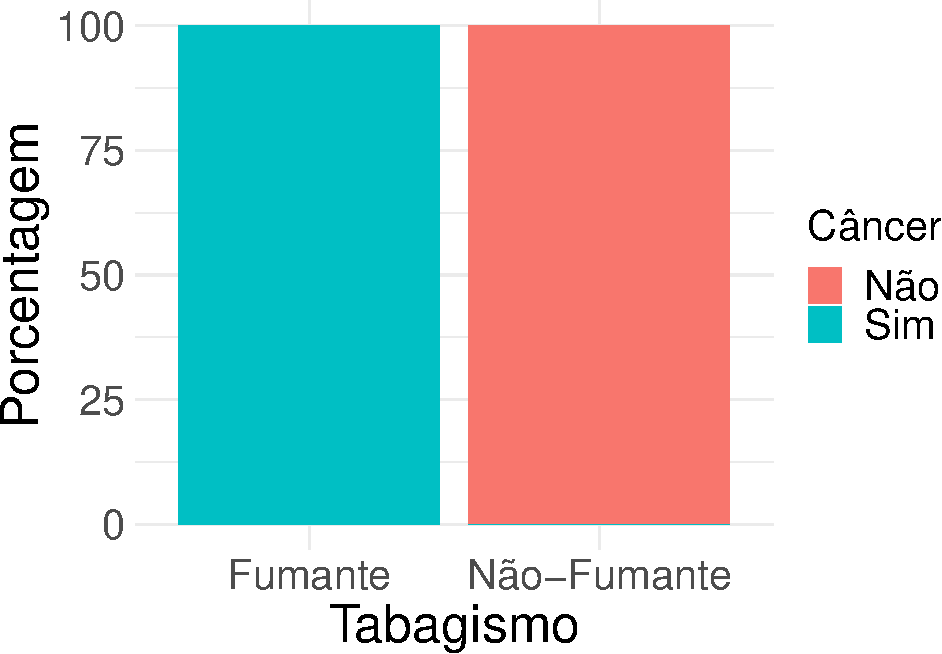
\includegraphics[width=0.5\linewidth]{relatorio_covid19_files/figure-latex/associacao-1} 

}

\caption{Associação entre Tabagismo e Câncer.}\label{fig:associacao}
\end{figure}

\hypertarget{exemplo-de-nuxe3o-associauxe7uxe3o-entre-duas-variuxe1veis-qualitativas}{%
\subsubsection{Exemplo de não associação entre duas variáveis qualitativas}\label{exemplo-de-nuxe3o-associauxe7uxe3o-entre-duas-variuxe1veis-qualitativas}}

Para ilustração vamos estudar um exempo de não associação hipotético do livro Barbetta (\protect\hyperlink{ref-barbetta2008estatistica}{2008}). Imagine que um pesquisador está interessado em estudar a associação entre as variáveis qualitativas \texttt{gênero} e \texttt{tabagismo} em uma amostra de \(300\) pessoas e obteve a tabela de contingência da Tabela \ref{tab:naoAssociacao}. A variável \texttt{gênero} tem duas categorias: \texttt{masculino} (a pessoa se identifica com o gênero masculino) e \texttt{feminino} (a pessoa se identifica com o gênero feminino). A variável \texttt{tabagismo} tem duas categorias: \texttt{fumante} (a pessoa tem o hábito de fumar) e \texttt{não-fumante} (a pessoa não tem o hábito de fumar).

\begin{table}[htbp]
\centering
\caption{Tabela de contingência para as Gênero e Tabagismo.}
\label{tab:naoAssociacao}
\begin{tabular}{l|cc|l}
& \multicolumn{2}{|c|}{Gênero} & \\ \cline{2-3}
Tabagismo & Masculino & Feminino & Total\\ \hline
Não-Fumante & 80 & 40 & 120\\
Fumante & 120 & 60 & 180\\ \hline
Total & 200 & 100 & 300\\
\end{tabular}
\end{table}

Calculando a frequência relativa por linha na Tabela \ref{tab:naoAssociacao}, obtemos as frequências relativas da Tabela \ref{tab:naoAssociacaoRel}.

\begin{table}[htbp]
\centering
\caption{Tabela de distribuição de frequência relativa ao total das colunas.}
\label{tab:naoAssociacaoRel}
\begin{tabular}{l|ll|l}
& \multicolumn{2}{|c|}{Gênero} & \\ \cline{2-3}
Tabagismo & Homem & Mulher & Total\\ \hline
Não-Fumante & {\color{brown} $\frac{80}{200}\cdot 100 = 40\%$} &  {\color{blue}$\frac{40}{100}\cdot 100 = 40\%$} & {\color{red}$\frac{120}{300}\cdot 100= 40\%$} \\
Fumante & $\frac{120}{200}\cdot 100 = 60\%$  &  $\frac{60}{100}\cdot 100= 60\%$ &  $\frac{180}{300}\cdot 100=60\%$ \\ \hline
Total & $\frac{200}{200}\cdot 100= 100\%$ &  $\frac{100}{100}\cdot 100 = 100\%$  & $\frac{300}{300}\cdot 100= 100\%$ \\ 
\end{tabular}
\end{table}

Na Tabela \ref{tab:naoAssociacaoRel}, notamos que os valores destacados em vermelho, azul e marrom são iguais. Se não sabemos o valor da variável \texttt{gênero} de um indivíduo, dizemos que uma pessoa tem aproximadamente \(40\%\) de probabilidade de ser fumante (conforme destacado em vermelhado). Contudo, ao descobrir / revelar / conhecer o valor da variável \texttt{gênero}, essa probabilidade permanece idêntica. Mais precisamente, se descobrirmos que a pessoa se identifica com o gênero feminino (\texttt{gênero} = \texttt{feminino}) então a probabilidade da pessoa fumar é aproximadamente \(40\%\) (cor azul), e se descobrirmos que a pessoa se identifica com o gênero masculino (\texttt{gênero} = \texttt{masculino}) então a probabildiade da pessoa fumar também é aproximadamente \(40\%\) (cor marrom). Ou seja, conhecer o valor \texttt{gênero} para uma pessoa não muda nem se altera as probabilidades dos valores de \texttt{tabagismo}, e então dizemos as duas variáveis qualitativas não estão associadas. Isto é, conhecer o valor da variável \texttt{gênero} não nos ajuda a descobrir ou determinar o valor (ou a probabilidade dos valores) da variável \texttt{tabagismo}. Geralmente, é conveniente representar a Tabela \ref{tab:naoAssociacaoRel} usando gráfico de barras conforme ilustrado na Figura \ref{fig:naoAssociacao}. Note que na Figura \ref{fig:naoAssociacao}, as duas barras são idênticas. De uma forma geral, se as barras iguais indicam uma não associação entre as variáveis qualitativas e barras diferentes indicam uma associação entre as variáveis qualitativas.

\begin{figure}[htbp]

{\centering 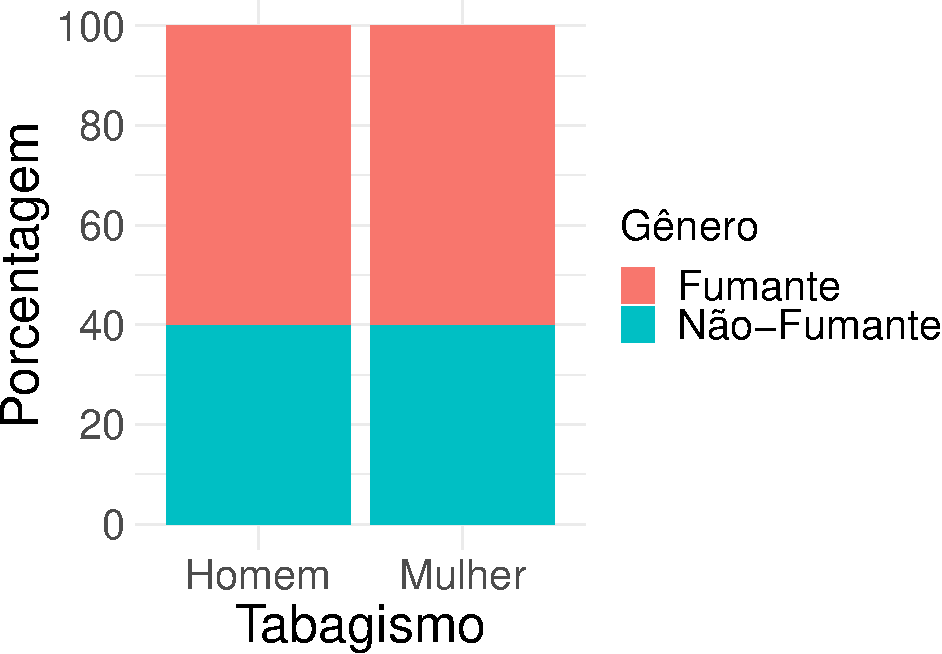
\includegraphics[width=0.5\linewidth]{relatorio_covid19_files/figure-latex/naoAssociacao-1} 

}

\caption{Não associação entre Gênero e Tabagismo.}\label{fig:naoAssociacao}
\end{figure}

\hypertarget{teste-qui-quadrado-1}{%
\subsubsection{Teste qui-quadrado}\label{teste-qui-quadrado-1}}

O teste qui-quadrado é geralmente usado para checar a associação entre duas variáveis
qualitativas. Considere as variáveis \(X\) e \(Y\) duas variáveis qualitativas da
Tabela \ref{tab:contingencia}, então, como já comentamos, se \(X\) e \(Y\) não são associadas temos que
\begin{equation}
\label{eq:quiQuadrado}
n_{ij} = \frac{n_{i \cdot } n_{\cdot j}}{n_{\cdot \cdot}} = \frac{\mbox{total da linha }i \cdot \mbox{total da colunha }j}{\mbox{tamanho da amostra}},
\end{equation}
em que \(n_{i \cdot}\) é o total da linha que corresponde ao valor \(A_i\) na Tabela \ref{tab:contingencia}, \(n_{\cdot j}\) é o total da colunha que corresponde ao valor \(B_j\) na Tabela \ref{tab:contingencia}, e \(n_{\cdot \cdot}\) é o tamanho da amostra.

Quando coletamos uma amostra não sabemos se duas variáveis estão associadas. Então, calculamos a expressão do lado direito da equação \eqref{eq:quiQuadrado}
\[
e_{ij} = \frac{\mbox{total da linha }i \cdot \mbox{total da colunha }j}{\mbox{tamanho da amostra}}
\]
e comparamos com o valor \(n_{ij}\) que obtemos da amostra. Chamamos \(e_{ij}\) de valor frequência esperada e \(n_{ij}\) de valor de frequência observada. Se as frequências esperadas e as frequência observadas forem iguais (ou estiverem próximas), podemos concluir que \(X\) e \(Y\) não estão associadas. Ou seja, se as distâncias padronizadas \(\frac{(e_{ij} - n_{ij})^2}{e_{ij}}\) entre \(e_{ij}\) e \(n_{ij}\) forem pequenas, então \(X\) e \(Y\) \textbf{não} estão associadas. Estas distâncias padronizadas são não-negativas, então \(X\) e \(Y\) \textbf{não} estão associadas se, e somente se, a soma de todas estas distâncias \(\frac{(e_{ij} - n_{ij})^2}{e_{ij}}\) são pequenas. Consequentemente, se
\[
\chi_0^2 = \sum_{i=1}^{r} \sum_{j=1}^{s} \frac{(e_{ij} - n_{ij})^2}{e_{ij}},
\]
for pequeno, então \(X\) e \(Y\) não estão associadas.

Para saber se \(\chi_0^2\) é pequeno ou grande, comparamos \(\chi_0^2\) o valor de quantil da distribuição qui-quadrado com \((r-1)(s-1)\) graus de liberdade (vide Montgomery and Runger \protect\hyperlink{ref-montgomery2010applied}{2010} para detalhes). Mais precisamente, queremos decidir entre as duas hipóteses científicas
\begin{align*}
H_0 &= \mbox{as duas variáveis qualitativas não estão associadas},\\
H_1 &= \mbox{as duas variáveis qualitativas estão associadas},
\end{align*}
e para isso fixamos o nível de significância \(\alpha\), calculamos o valor-p \(p\) e rejeitamos \(H_0\) se \(p < \alpha\) (vide Spiegel et al. \protect\hyperlink{ref-spiegel2001probability}{2001} para detalhes sobre valor-p). Neste relatório, vamos usar o nível de significânica \(\alpha=0,01\) .

\hypertarget{teste-kruskal-wallis}{%
\subsection{Teste Kruskal-Wallis}\label{teste-kruskal-wallis}}

Usamos o Teste Kruskal-Wallis para comparar populações, através da mediana, onde não é adequado assumir a distribuição normal, como é caso escalas Likert. Neste teste, supomos que temos \(k\) populações e para cada população \(j,\ j=1, \dots, k,\) coletamos uma amostra de tamanho \(n_j\), ou seja, a amostra completa com as crianças de todas as populações tem \(N = n_1 + \dots + n_k\) crianças. Seja \(X_{ij}\) é a resposta da criança \(i\) da população \(j\), então
\[
X_{ij} = \theta + \tau_j + \epsilon_{ij}, \qquad  j=1, \dots, k,\qquad i=1, \dots, n_j,
\]
onde \(\theta\) é a mediana da amostra completa, \(\tau_j\) é o efeito de tratamento da \(j\)-ésima população e \(\epsilon_{ij}\) são erros aleatórios com mediana igual a zero, e queremos decidir entre duas hipóteses
\[
\begin{split}
&H_0: \tau_1 = \tau_2 = \dots = \tau_j,\\
&H_1: \tau_1, \tau_2, \dots,  \tau_j \mbox{ não são todos iguais}.
\end{split}
\]
e para isso fixamos o nível de significância \(\alpha\), calculamos o valor-p \(p\) e rejeitamos \(H_0\) se \(p < \alpha\) (vide Spiegel et al. \protect\hyperlink{ref-spiegel2001probability}{2001} para detalhes sobre valor-p). Neste relatório, vamos usar o nível de significânica \(\alpha=0,01\).

Para detalhes sobre o teste Kruskal-Wallis, recomendo a leitura de Hollander, Wolfe, and Chicken (\protect\hyperlink{ref-hollander2013nonparametric}{2013}).

\hypertarget{teste-de-comparauxe7uxe3o-muxfaltipla-de-nemeyi}{%
\subsection{Teste de comparação múltipla de Nemeyi}\label{teste-de-comparauxe7uxe3o-muxfaltipla-de-nemeyi}}

O teste de Nemeyi (Nemenyi \protect\hyperlink{ref-nemenyi1963distribution}{1963}) é teste \emph{posthoc} de comparação múltipla que pode ser usada para identificar pares têm medianas diferentes populações se o teste de Kruskal-Wallis indica que as medianas das populações não são todas iguais. O teste consiste em realizar comparações em pares para identificar quais populações tem medianas diferentes.

O número de comparações de medianas realizadas é \(\frac{k(k-1)}{2}\), e o teste foi construído em soma de postos e na aplicação do método \emph{family-wise-error} para controlar a inflação do erro tipo I se várias comparações forem feitas. E para cada par de populações queremos decidir entre as hipóteses:
\[
\begin{split}
&H_0: m_l = m_j\\
&H_1: m_l \neq m_j
\end{split}
\]
onde \(m_l\) é a mediana da população \(l\) e \(m_j\) é a mediana da população \(j\). Para decidirmos entre estas hipóteses, fixamos o nível de significância \(\alpha\), calculamos o valor-p \(p\) e rejeitamos \(H_0\) se \(p < \alpha\) (vide Spiegel et al. \protect\hyperlink{ref-spiegel2001probability}{2001} para detalhes sobre valor-p). Neste relatório, vamos usar o nível de significânica \(\alpha=0,01\).

Para detalhes sobre o teste de comparação múltipla de Nemeyi, recomendo a leitura da vinheta do pacote da liguagem Pohlert (\protect\hyperlink{ref-PMCMR}{2014}).

\hypertarget{arquivos-suplementares}{%
\subsection{Arquivos suplementares}\label{arquivos-suplementares}}

Para facilitar a redação de relatórios e artigos pelas consulentes, coloco em anexo os seguintes arquivos:

\begin{itemize}
\tightlist
\item
  \texttt{output.zip}: este arquivo contém o sequintes diretórios

  \begin{itemize}
  \tightlist
  \item
    \texttt{kruskal\_wallis\_test}: diretório com arquivos \texttt{.csv} e \texttt{.xlsx} com os testes Kruskal-Wallis
  \item
    \texttt{medidas\_resumos\_bidimensional}: diretório com arquivos \texttt{.csv} e \texttt{.xlsx} com medidas de resumo calculas de cada grupo de uma variável categórica
  \item
    \texttt{medidas\_resumos\_unidimensional}: diretório com arquivos \texttt{.csv} e \texttt{.xlsx} com medidas de resumo para cada uma das variáveis neste relatório
  \item
    \texttt{nemenyi\_tests}: diretório com arquivos \texttt{.csv} e \texttt{.xlsx} com os valores-p do teste de comparação múltipla de Nemeyi
  \item
    \texttt{tabela\_contingencia}: diretório com arquivos \texttt{.csv} e \texttt{.xlsx} com as tabelas de contingências
  \item
    \texttt{tabela\_distribuicao}: diretório com arquivos \texttt{.csv} e \texttt{.xlsx} com as tabelas de distribuições de frequências para as variáveis categóricas
  \item
    \texttt{teste\_qui\_quadrado}: diretório com arquivos \texttt{.csv} e \texttt{.xlsx} com os testes qui-quadrado
  \end{itemize}
\item
  \texttt{figuras.zip}: este arquivo contém os seguintes diretórios:

  \begin{itemize}
  \tightlist
  \item
    \texttt{boxplot\_bidimensional}: diretório com figuras nos formatos \texttt{.png} e \texttt{.pdf} com o diagrama de caixa (boxplot) de cada grupo da variável categórica
  \item
    \texttt{grafico\_barra\_bidimensional}: diretório com figuras nos formatos \texttt{.png} e \texttt{.pdf} com gráfico de barras para duas variáveis categóricas
  \item
    \texttt{grafico\_barra\_unidimensional}: diretório com figuras nos formatos \texttt{.png} e \texttt{.pdf} com gráfico de barras para cada variável categórica
  \end{itemize}
\end{itemize}

\cleardoublepage

\hypertarget{resultados}{%
\section{Resultados}\label{resultados}}

Dividimos esta seção em duas partes. Começamos com a análise descritiva para as seguintes variávies categóricas:

\begin{enumerate}
\def\labelenumi{\roman{enumi}.}
\tightlist
\item
  Idade
\item
  Tipo de escola
\item
  Gênero
\item
  Raça
\item
  Cidades
\end{enumerate}

Nesta parte, apresentamos as tabelas de distribuição de frequências e o gráfico de barras sem comentários adicionais. Em seguida, comparamos as escalas de Likert por cada grupo especificado pelas variáveis categóricas elencadas acima. Nesta última parte, também seremos lacônicos, pois este consultar acredita que as consulentes são qualificadas para dar uma interpretação adequada aos resultados dos métodos estatísticos e para tentar diminuir o número de páginas deste relatório.

\cleardoublepage

\hypertarget{q14}{%
\subsection{Q14}\label{q14}}

A variável Q14 corresponde ao campo de númeo 13 com enunciado \textbf{O quanto você está preocupado hoje com as questões abaixo} no quesito:

\begin{itemize}
\tightlist
\item
  \emph{Que minha família e meus amigos fiquem mais pobres, com menos dinheiro ou sem emprego}
\end{itemize}

\hypertarget{anuxe1lise-descritiva-para-q14}{%
\subsubsection{Análise descritiva para Q14}\label{anuxe1lise-descritiva-para-q14}}

\hypertarget{gruxe1fico-de-barras-q14}{%
\paragraph{Gráfico de barras: Q14}\label{gruxe1fico-de-barras-q14}}

\begin{center}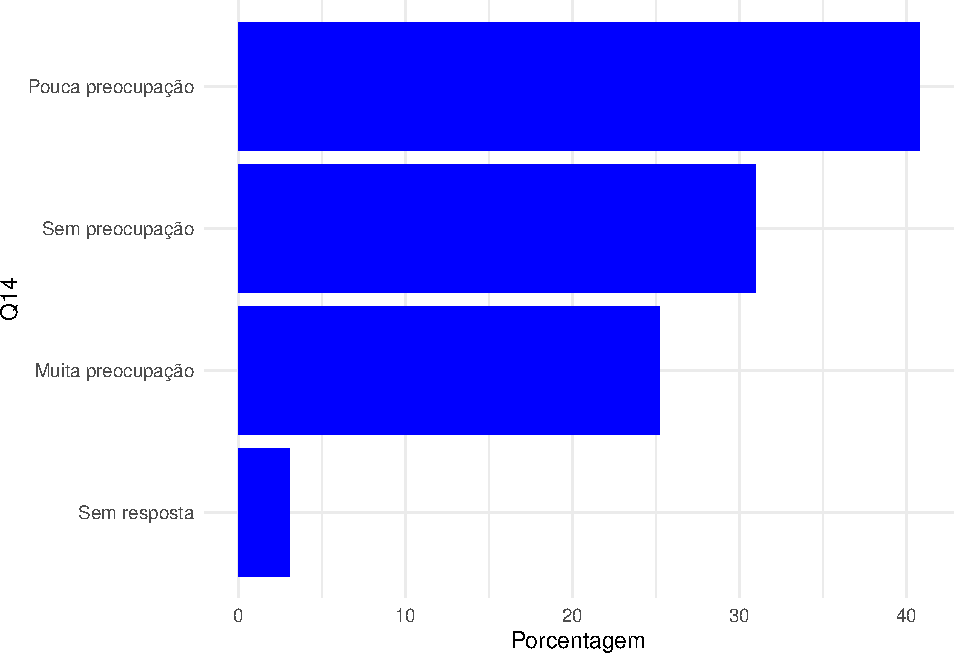
\includegraphics[width=0.75\linewidth]{relatorio_covid19_files/figure-latex/unnamed-chunk-10-1} \end{center}

\hypertarget{tabela-de-distribuiuxe7uxe3o-q14}{%
\paragraph{Tabela de distribuição: Q14}\label{tabela-de-distribuiuxe7uxe3o-q14}}

\begin{longtable}[]{@{}cccc@{}}
\caption{\label{tab:unnamed-chunk-11}Que minha família e meus amigos fiquem mais pobres, com menos dinheiro ou sem emprego}\tabularnewline
\toprule
Q14 & Frequência & Frequência relativa & Porcentagem\tabularnewline
\midrule
\endfirsthead
\toprule
Q14 & Frequência & Frequência relativa & Porcentagem\tabularnewline
\midrule
\endhead
Pouca preocupação & 428 & 0,41 & 40,76\tabularnewline
Sem preocupação & 325 & 0,31 & 30,95\tabularnewline
Muita preocupação & 265 & 0,25 & 25,24\tabularnewline
Sem resposta & 32 & 0,03 & 3,05\tabularnewline
\bottomrule
\end{longtable}

\hypertarget{medidas-de-resumo-q14}{%
\paragraph{Medidas de resumo: Q14}\label{medidas-de-resumo-q14}}

\begin{longtable}[]{@{}ccccc@{}}
\caption{\label{tab:unnamed-chunk-12}Resumos para variável Q14.}\tabularnewline
\toprule
Média & Desvio Padrão & Mediana & 1Qua & 3Qua\tabularnewline
\midrule
\endfirsthead
\toprule
Média & Desvio Padrão & Mediana & 1Qua & 3Qua\tabularnewline
\midrule
\endhead
1 & 0,83 & 1 & 0 & 2\tabularnewline
\bottomrule
\end{longtable}

\cleardoublepage

\hypertarget{anuxe1lise-bidimensional-q14}{%
\subsubsection{Análise bidimensional Q14}\label{anuxe1lise-bidimensional-q14}}

\hypertarget{tabela-de-continguxeancia-cidade-e-q14}{%
\paragraph{Tabela de contingência: Cidade e Q14}\label{tabela-de-continguxeancia-cidade-e-q14}}

\begin{longtable}[]{@{}ccccc@{}}
\caption{\label{tab:unnamed-chunk-13}Tabela de contingência: Cidade e Q14.}\tabularnewline
\toprule
Cidade & Muita preocupação & Pouca preocupação & Sem preocupação & Sem resposta\tabularnewline
\midrule
\endfirsthead
\toprule
Cidade & Muita preocupação & Pouca preocupação & Sem preocupação & Sem resposta\tabularnewline
\midrule
\endhead
Camaçari & 72 & 77 & 40 & 8\tabularnewline
Candeias & 12 & 15 & 9 & 2\tabularnewline
Lauro de Freitas & 11 & 26 & 23 & 1\tabularnewline
Outros & 23 & 41 & 19 &\tabularnewline
Pojuca & 25 & 27 & 10 & 2\tabularnewline
Salvador & 113 & 225 & 217 & 18\tabularnewline
Simões Filho & 9 & 17 & 7 & 1\tabularnewline
\bottomrule
\end{longtable}

\hypertarget{gruxe1fico-de-barras-cidade-e-q14}{%
\paragraph{Gráfico de barras: Cidade e Q14}\label{gruxe1fico-de-barras-cidade-e-q14}}

\begin{center}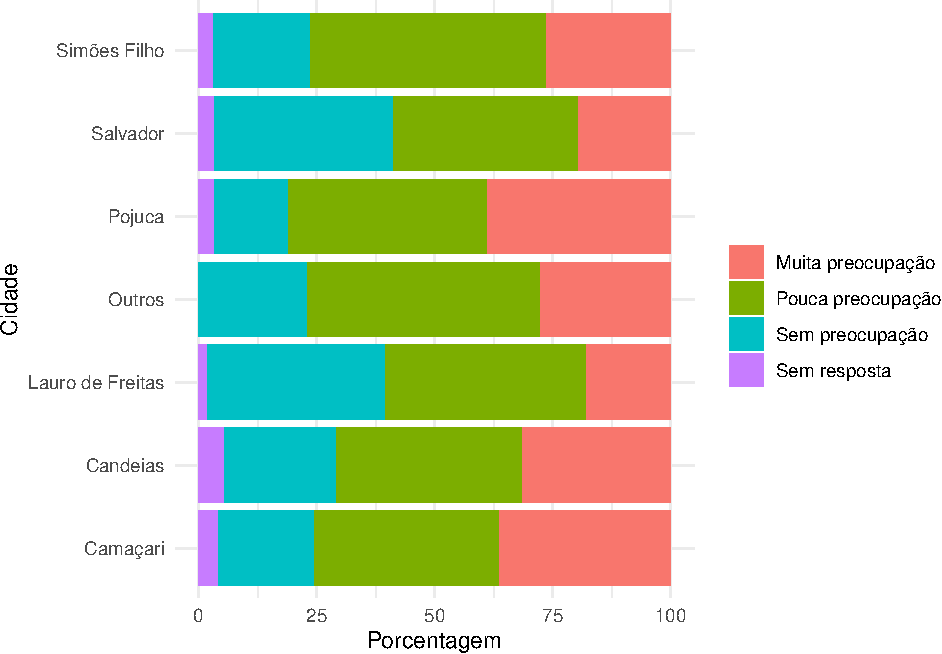
\includegraphics[width=0.75\linewidth]{relatorio_covid19_files/figure-latex/unnamed-chunk-14-1} \end{center}

\hypertarget{teste-qui-quadrado-2}{%
\paragraph{Teste qui-quadrado}\label{teste-qui-quadrado-2}}

Como o valor-p é menor que 0.01 (nível de significância), rejeitamos a hipótese nula e temos evidência estatística que as duas variáveis estão associadas.

\begin{longtable}[]{@{}ccc@{}}
\caption{\label{tab:unnamed-chunk-16}Teste qui-quadrado entre Cidade e Q14.}\tabularnewline
\toprule
Estatística & Graus de liberdade & Valor-p\tabularnewline
\midrule
\endfirsthead
\toprule
Estatística & Graus de liberdade & Valor-p\tabularnewline
\midrule
\endhead
56,23 & 18 & 0\tabularnewline
\bottomrule
\end{longtable}

\cleardoublepage

\hypertarget{medidas-de-resumo-q14-por-cidade}{%
\paragraph{Medidas de Resumo Q14 por Cidade}\label{medidas-de-resumo-q14-por-cidade}}

\begin{longtable}[]{@{}cccccc@{}}
\caption{\label{tab:unnamed-chunk-17}Medidas de resumo de Q14 por Cidade.}\tabularnewline
\toprule
Q14 & Média & Desvio Padrão & Mediana & 1 Quartil & 3 Quartil\tabularnewline
\midrule
\endfirsthead
\toprule
Q14 & Média & Desvio Padrão & Mediana & 1 Quartil & 3 Quartil\tabularnewline
\midrule
\endhead
Camaçari & 1,24 & 0,82 & 1 & 1 & 2\tabularnewline
Candeias & 1,18 & 0,87 & 1 & 1 & 2\tabularnewline
Lauro de Freitas & 0,84 & 0,78 & 1 & 0 & 1\tabularnewline
Outros & 1,05 & 0,71 & 1 & 1 & 2\tabularnewline
Pojuca & 1,30 & 0,77 & 1 & 1 & 2\tabularnewline
Salvador & 0,88 & 0,83 & 1 & 0 & 1\tabularnewline
Simões Filho & 1,12 & 0,77 & 1 & 1 & 2\tabularnewline
\bottomrule
\end{longtable}

\hypertarget{boxplot-de-q14-por-cidade}{%
\paragraph{Boxplot de Q14 por Cidade}\label{boxplot-de-q14-por-cidade}}

\begin{center}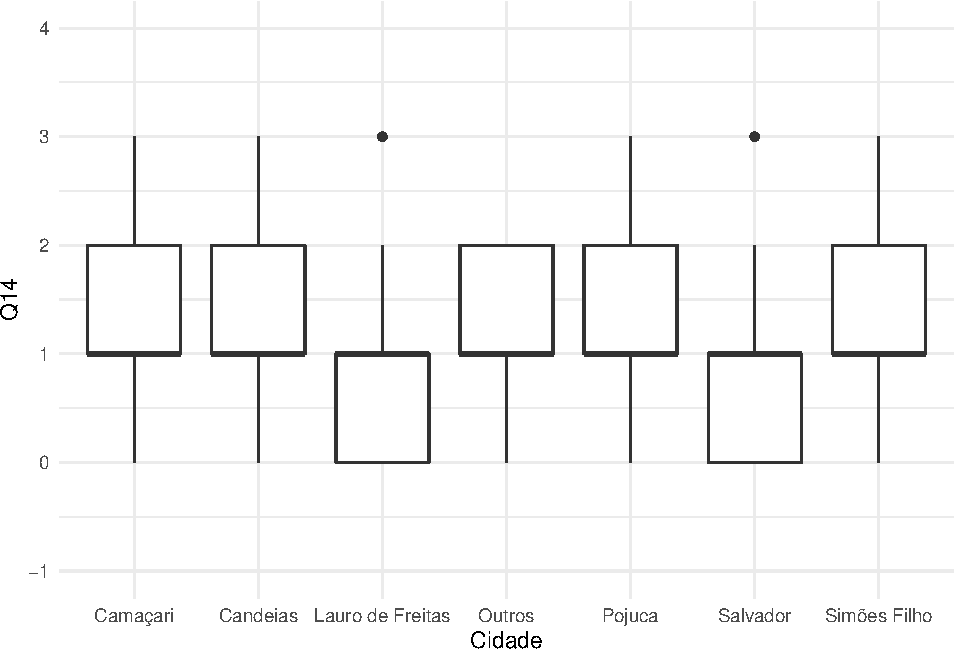
\includegraphics[width=0.75\linewidth]{relatorio_covid19_files/figure-latex/unnamed-chunk-18-1} \end{center}

\hypertarget{teste-de-kruskal-wallis-de-q14-por-cidade}{%
\paragraph{Teste de Kruskal-Wallis de Q14 por Cidade}\label{teste-de-kruskal-wallis-de-q14-por-cidade}}

Como o valor-p é menor que 0.01 (nível de significância), rejeitamos a hipótese nula e as medianas de Q14 entre as crianças de diversas cidades não são todas iguais.

\begin{longtable}[]{@{}ccc@{}}
\caption{\label{tab:unnamed-chunk-20}Valor-p para o teste de Kruskal-Wallis: Q14 e Cidade.}\tabularnewline
\toprule
Estatística & Parâmetro & valor p\tabularnewline
\midrule
\endfirsthead
\toprule
Estatística & Parâmetro & valor p\tabularnewline
\midrule
\endhead
45,53 & 6 & 0\tabularnewline
\bottomrule
\end{longtable}

\hypertarget{teste-de-nemeyi-de-q14-por-cidade}{%
\paragraph{Teste de Nemeyi de Q14 por Cidade}\label{teste-de-nemeyi-de-q14-por-cidade}}

Existem valores-p menores que 0.01 (nível de significância), e para estes pares rejeitamos a hipótese nula e as medianas de Q14 entre as crianças destes pares de cidades são diferentes.

\begin{longtable}[]{@{}lcccccc@{}}
\caption{\label{tab:unnamed-chunk-22}Valores-p para o teste de comparação múltipla de Nemeyi de Q14 por Cidade.}\tabularnewline
\toprule
& Camaçari & Candeias & Lauro de Freitas & Outros & Pojuca & Salvador\tabularnewline
\midrule
\endfirsthead
\toprule
& Camaçari & Candeias & Lauro de Freitas & Outros & Pojuca & Salvador\tabularnewline
\midrule
\endhead
Candeias & 1,00 & & & & &\tabularnewline
Lauro de Freitas & 0,02 & 0,50 & & & &\tabularnewline
Outros & 0,73 & 1,00 & 0,69 & & &\tabularnewline
Pojuca & 1,00 & 0,99 & 0,04 & 0,66 & &\tabularnewline
Salvador & 0,00 & 0,37 & 1,00 & 0,46 & 0,00 &\tabularnewline
Simões Filho & 0,99 & 1,00 & 0,72 & 1,00 & 0,96 & 0,66\tabularnewline
\bottomrule
\end{longtable}

\cleardoublepage

\hypertarget{tabela-de-continguxeancia-guxeanero-e-q14}{%
\paragraph{Tabela de contingência: Gênero e Q14}\label{tabela-de-continguxeancia-guxeanero-e-q14}}

Apenas seis crianças se identificaram com o gênero \emph{outros} e foram removidas na análise estatística.

\begin{longtable}[]{@{}ccccc@{}}
\caption{\label{tab:unnamed-chunk-23}Tabela de contingência: Gênero e Q14.}\tabularnewline
\toprule
Gênero & Muita preocupação & Pouca preocupação & Sem preocupação & Sem resposta\tabularnewline
\midrule
\endfirsthead
\toprule
Gênero & Muita preocupação & Pouca preocupação & Sem preocupação & Sem resposta\tabularnewline
\midrule
\endhead
Menina & 134 & 227 & 162 & 18\tabularnewline
Menino & 131 & 196 & 162 & 14\tabularnewline
\bottomrule
\end{longtable}

\hypertarget{gruxe1fico-de-barras-guxeanero-e-q14}{%
\paragraph{Gráfico de barras: Gênero e Q14}\label{gruxe1fico-de-barras-guxeanero-e-q14}}

Apenas seis crianças se identificaram com o gênero \emph{outros} e foram removidas na análise estatística.

\begin{center}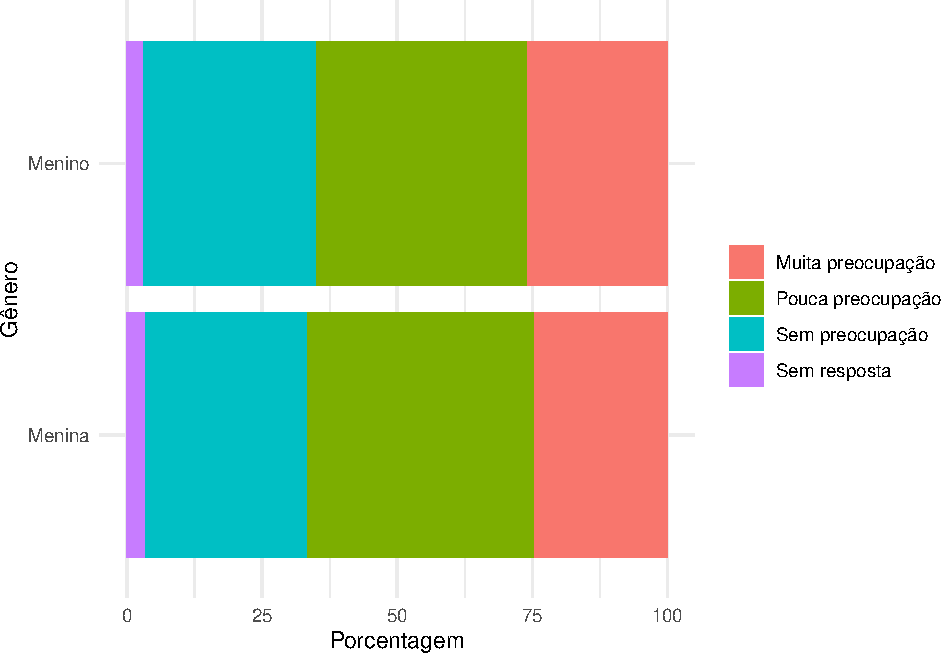
\includegraphics[width=0.75\linewidth]{relatorio_covid19_files/figure-latex/unnamed-chunk-24-1} \end{center}

\hypertarget{teste-qui-quadrado-3}{%
\paragraph{Teste qui-quadrado}\label{teste-qui-quadrado-3}}

Apenas seis crianças se identificaram com o gênero \emph{outros} e foram removidas na análise estatística.

Como o valor-p é igual ou maior que 0.01 (nível de significância), não rejeitamos a hipótese nula e não temos evidência estatística que as duas variáveis estão associadas.

\begin{longtable}[]{@{}ccc@{}}
\caption{\label{tab:unnamed-chunk-26}Teste qui-quadrado entre Gênero e Q14.}\tabularnewline
\toprule
Estatística & Graus de liberdade & Valor-p\tabularnewline
\midrule
\endfirsthead
\toprule
Estatística & Graus de liberdade & Valor-p\tabularnewline
\midrule
\endhead
1,42 & 3 & 0,7\tabularnewline
\bottomrule
\end{longtable}

\cleardoublepage

\hypertarget{medidas-de-resumo-q14-por-guxeanero}{%
\paragraph{Medidas de Resumo Q14 por Gênero}\label{medidas-de-resumo-q14-por-guxeanero}}

Apenas seis crianças se identificaram com o gênero \emph{outros} e foram removidas na análise estatística.

\begin{longtable}[]{@{}cccccc@{}}
\caption{\label{tab:unnamed-chunk-27}Medidas de resumo de Q14 por Gênero.}\tabularnewline
\toprule
Q14 & Média & Desvio Padrão & Mediana & 1 Quartil & 3 Quartil\tabularnewline
\midrule
\endfirsthead
\toprule
Q14 & Média & Desvio Padrão & Mediana & 1 Quartil & 3 Quartil\tabularnewline
\midrule
\endhead
Menina & 1,01 & 0,83 & 1 & 0 & 2\tabularnewline
Menino & 0,99 & 0,83 & 1 & 0 & 2\tabularnewline
\bottomrule
\end{longtable}

\hypertarget{boxplot-de-q14-por-guxeanero}{%
\paragraph{Boxplot de Q14 por Gênero}\label{boxplot-de-q14-por-guxeanero}}

Apenas seis crianças se identificaram com o gênero \emph{outros} e foram removidas na análise estatística.

\begin{center}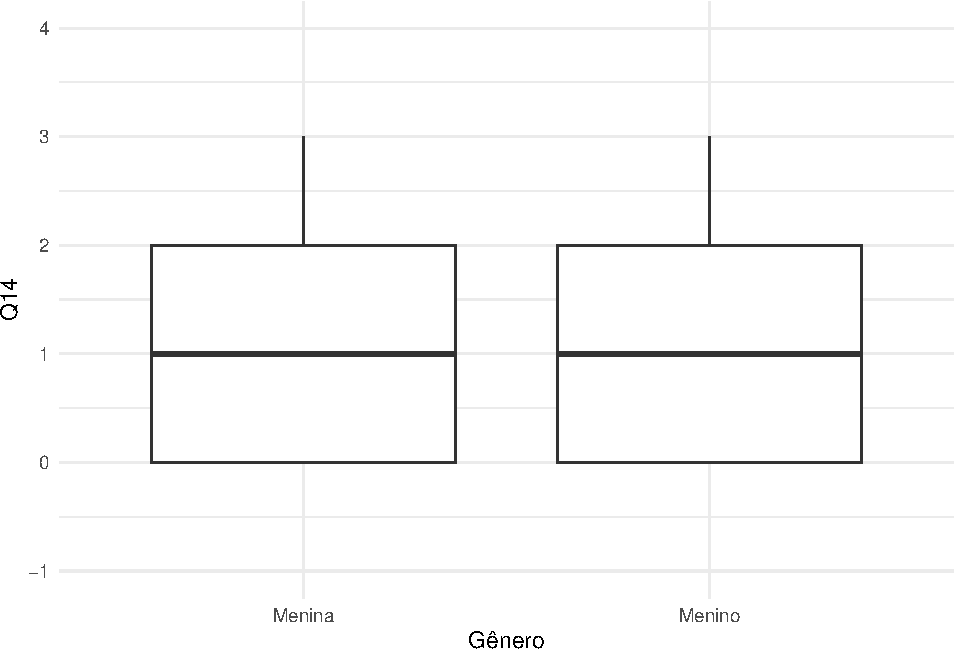
\includegraphics[width=0.75\linewidth]{relatorio_covid19_files/figure-latex/unnamed-chunk-28-1} \end{center}

\hypertarget{teste-de-kruskal-wallis-de-q14-por-guxeanero}{%
\paragraph{Teste de Kruskal-Wallis de Q14 por Gênero}\label{teste-de-kruskal-wallis-de-q14-por-guxeanero}}

Apenas seis crianças se identificaram com o gênero \emph{outros} e foram removidas na análise estatística.

Como o valor-p é maior ou igual a 0.01 (nível de significância), não rejeitamos a hipótese nula e as medianas de Q14 entre meninos e meninas são iguais.

\begin{longtable}[]{@{}ccc@{}}
\caption{\label{tab:unnamed-chunk-30}Valores-p para comparação múltipla de medianas: Q14 e Gênero.}\tabularnewline
\toprule
Estatística & Parâmetro & valor p\tabularnewline
\midrule
\endfirsthead
\toprule
Estatística & Parâmetro & valor p\tabularnewline
\midrule
\endhead
0,15 & 1 & 0,7\tabularnewline
\bottomrule
\end{longtable}

\hypertarget{teste-de-nemeyi-de-q14-por-guxeanero}{%
\paragraph{Teste de Nemeyi de Q14 por Gênero}\label{teste-de-nemeyi-de-q14-por-guxeanero}}

Apenas seis crianças se identificaram com o gênero \emph{outros} e foram removidas na análise estatística.

Como os valores-p são iguais ou maiores que 0.01 (nível de significância), não rejeitamos a hipótese nula e as medianas de Q14 entre meninos e meninas são iguais.

\begin{longtable}[]{@{}lc@{}}
\caption{\label{tab:unnamed-chunk-32}valores-p para o teste de comparação múltipla de Nemeyi de Q14 por Gênero.}\tabularnewline
\toprule
& Menina\tabularnewline
\midrule
\endfirsthead
\toprule
& Menina\tabularnewline
\midrule
\endhead
Menino & 0,72\tabularnewline
\bottomrule
\end{longtable}

\cleardoublepage

\hypertarget{tabela-de-continguxeancia-idade-e-q14}{%
\paragraph{Tabela de contingência: Idade e Q14}\label{tabela-de-continguxeancia-idade-e-q14}}

\begin{longtable}[]{@{}ccccc@{}}
\caption{\label{tab:unnamed-chunk-33}Tabela de contingência: Idade e Q14.}\tabularnewline
\toprule
Idade & Muita preocupação & Pouca preocupação & Sem preocupação & Sem resposta\tabularnewline
\midrule
\endfirsthead
\toprule
Idade & Muita preocupação & Pouca preocupação & Sem preocupação & Sem resposta\tabularnewline
\midrule
\endhead
8 & 52 & 78 & 59 & 6\tabularnewline
9 & 57 & 69 & 58 & 2\tabularnewline
10 & 68 & 100 & 68 & 14\tabularnewline
11 & 49 & 109 & 74 & 8\tabularnewline
12 & 39 & 72 & 66 & 2\tabularnewline
\bottomrule
\end{longtable}

\hypertarget{gruxe1fico-de-barras-idade-e-q14}{%
\paragraph{Gráfico de barras: Idade e Q14}\label{gruxe1fico-de-barras-idade-e-q14}}

\begin{center}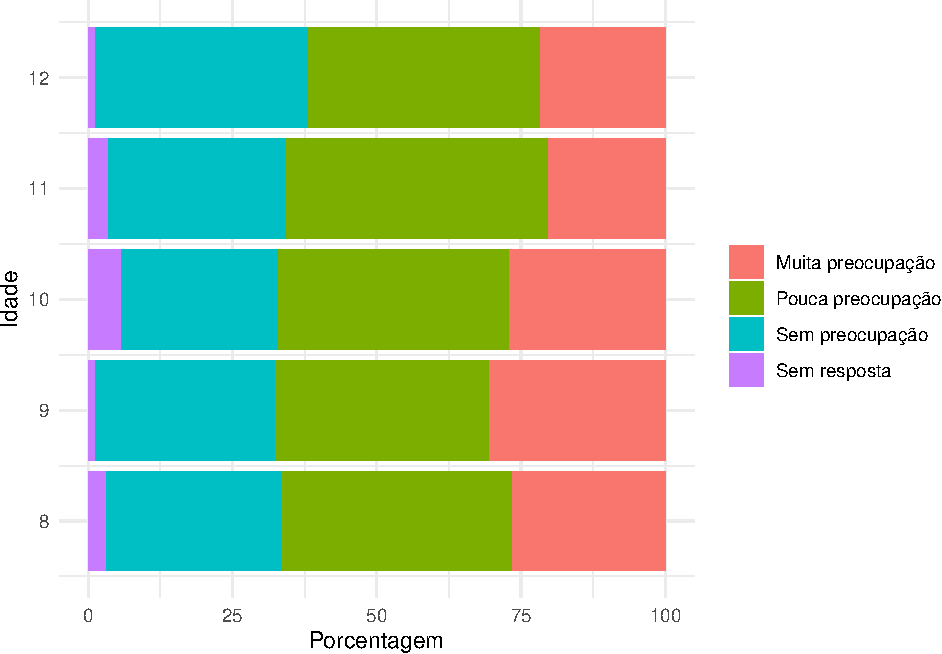
\includegraphics[width=0.75\linewidth]{relatorio_covid19_files/figure-latex/unnamed-chunk-34-1} \end{center}

\hypertarget{teste-qui-quadrado-4}{%
\paragraph{Teste qui-quadrado}\label{teste-qui-quadrado-4}}

Como o valor-p é igual ou maior que 0.01 (nível de significância), não rejeitamos a hipótese nula e não temos evidência estatística que as duas variáveis estão associadas.

\begin{longtable}[]{@{}ccc@{}}
\caption{\label{tab:unnamed-chunk-36}Teste qui-quadrado entre Idade e Q14.}\tabularnewline
\toprule
Estatística & Graus de liberdade & Valor-p\tabularnewline
\midrule
\endfirsthead
\toprule
Estatística & Graus de liberdade & Valor-p\tabularnewline
\midrule
\endhead
20,88 & 12 & 0,05\tabularnewline
\bottomrule
\end{longtable}

\cleardoublepage

\hypertarget{medidas-de-resumo-q14-por-idade}{%
\paragraph{Medidas de Resumo Q14 por Idade}\label{medidas-de-resumo-q14-por-idade}}

\begin{longtable}[]{@{}cccccc@{}}
\caption{\label{tab:unnamed-chunk-37}Medidas de resumo de Q14 por Idade.}\tabularnewline
\toprule
Q14 & Média & Desvio Padrão & Mediana & 1 Quartil & 3 Quartil\tabularnewline
\midrule
\endfirsthead
\toprule
Q14 & Média & Desvio Padrão & Mediana & 1 Quartil & 3 Quartil\tabularnewline
\midrule
\endhead
8 & 1,03 & 0,83 & 1 & 0 & 2\tabularnewline
9 & 1,02 & 0,82 & 1 & 0 & 2\tabularnewline
10 & 1,11 & 0,87 & 1 & 0 & 2\tabularnewline
11 & 0,96 & 0,80 & 1 & 0 & 1\tabularnewline
12 & 0,87 & 0,79 & 1 & 0 & 1\tabularnewline
\bottomrule
\end{longtable}

\hypertarget{boxplot-de-q14-por-idade}{%
\paragraph{Boxplot de Q14 por Idade}\label{boxplot-de-q14-por-idade}}

\begin{center}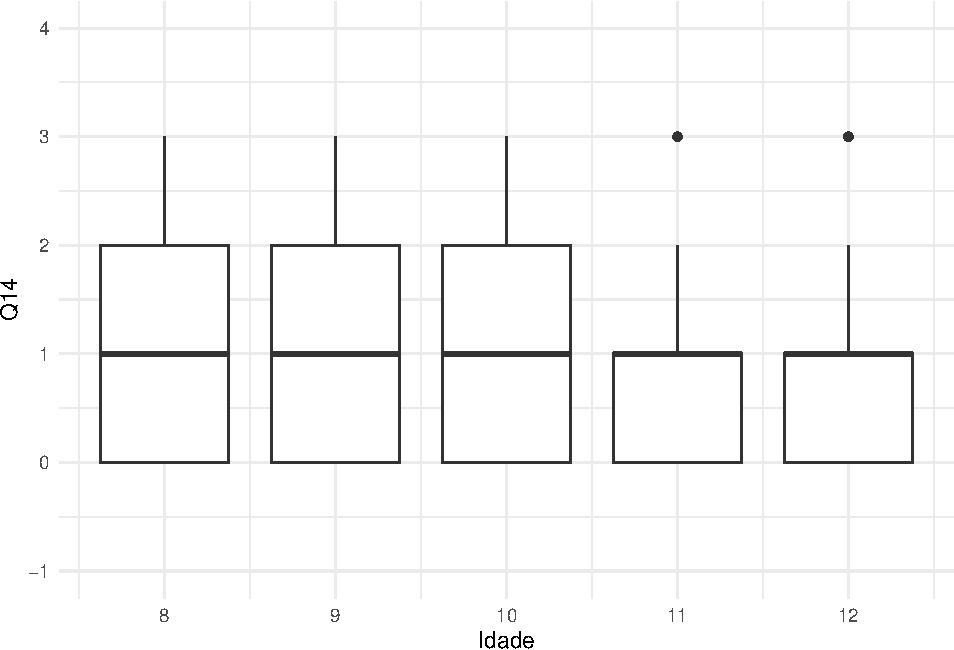
\includegraphics[width=0.75\linewidth]{relatorio_covid19_files/figure-latex/unnamed-chunk-38-1} \end{center}

\hypertarget{teste-de-kruskal-wallis-de-q14-por-idade}{%
\paragraph{Teste de Kruskal-Wallis de Q14 por Idade}\label{teste-de-kruskal-wallis-de-q14-por-idade}}

Como o valor-p é maior ou igual a 0.01 (nível de significância), não rejeitamos a hipótese nula e as medianas de Q14 entre as idades são iguais.

\begin{longtable}[]{@{}ccc@{}}
\caption{\label{tab:unnamed-chunk-40}Valores-p para comparação múltipla de medianas: Q14 e Idade.}\tabularnewline
\toprule
Estatística & Parâmetro & valor p\tabularnewline
\midrule
\endfirsthead
\toprule
Estatística & Parâmetro & valor p\tabularnewline
\midrule
\endhead
8,61 & 4 & 0,07\tabularnewline
\bottomrule
\end{longtable}

\hypertarget{teste-de-nemeyi-de-q14-por-idade}{%
\paragraph{Teste de Nemeyi de Q14 por Idade}\label{teste-de-nemeyi-de-q14-por-idade}}

Como os valores-p são iguais ou maiores que 0.01 (nível de significância), não rejeitamos a hipótese nula e as medianas de Q14 entre pares de crianças de diferentes idades são todas iguais.

\begin{longtable}[]{@{}lcccc@{}}
\caption{\label{tab:unnamed-chunk-42}Teste de Nemeyi de Q14 por Idade.}\tabularnewline
\toprule
& 8 & 9 & 10 & 11\tabularnewline
\midrule
\endfirsthead
\toprule
& 8 & 9 & 10 & 11\tabularnewline
\midrule
\endhead
9 & 1,00 & & &\tabularnewline
10 & 0,90 & 0,91 & &\tabularnewline
11 & 0,94 & 0,94 & 0,39 &\tabularnewline
12 & 0,47 & 0,48 & 0,07 & 0,87\tabularnewline
\bottomrule
\end{longtable}

\cleardoublepage

\hypertarget{tabela-de-continguxeancia-rauxe7a-e-q14}{%
\paragraph{Tabela de contingência: Raça e Q14}\label{tabela-de-continguxeancia-rauxe7a-e-q14}}

\begin{longtable}[]{@{}ccccc@{}}
\caption{\label{tab:unnamed-chunk-43}Tabela de contingência: Raça e Q14.}\tabularnewline
\toprule
Raça & Muita preocupação & Pouca preocupação & Sem preocupação & Sem resposta\tabularnewline
\midrule
\endfirsthead
\toprule
Raça & Muita preocupação & Pouca preocupação & Sem preocupação & Sem resposta\tabularnewline
\midrule
\endhead
Amarela & 2 & 7 & 7 & 3\tabularnewline
Branca & 41 & 76 & 95 & 1\tabularnewline
Indígena & 5 & 11 & 4 & 1\tabularnewline
Negra & 208 & 318 & 197 & 26\tabularnewline
Outros & 5 & 4 & 7 &\tabularnewline
Sem resposta & 4 & 12 & 15 & 1\tabularnewline
\bottomrule
\end{longtable}

\hypertarget{gruxe1fico-de-barras-rauxe7a-e-q14}{%
\paragraph{Gráfico de barras: Raça e Q14}\label{gruxe1fico-de-barras-rauxe7a-e-q14}}

\begin{center}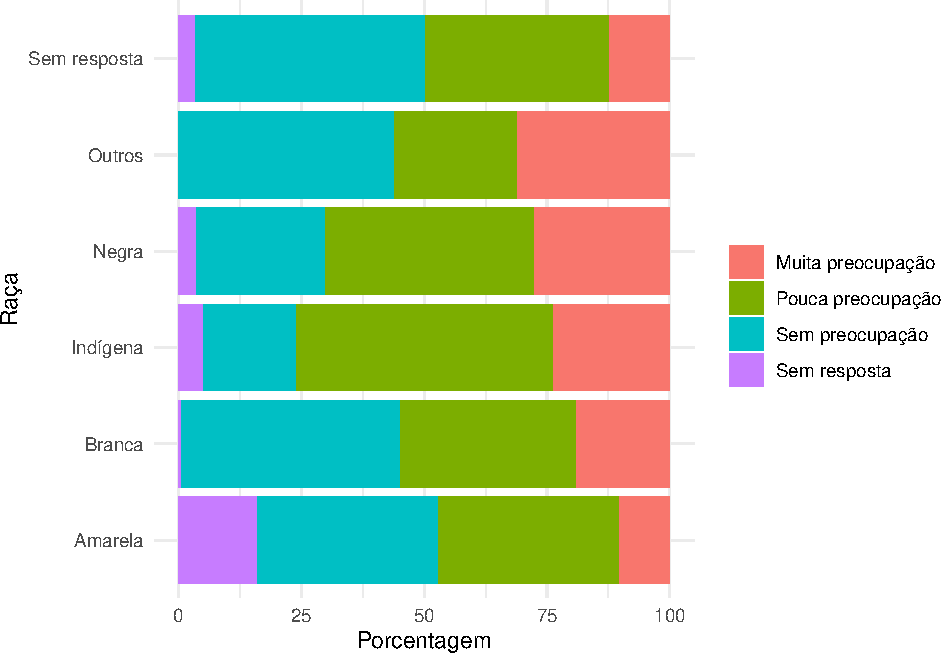
\includegraphics[width=0.75\linewidth]{relatorio_covid19_files/figure-latex/unnamed-chunk-44-1} \end{center}

\hypertarget{teste-qui-quadrado-5}{%
\paragraph{Teste qui-quadrado}\label{teste-qui-quadrado-5}}

Como o valor-p é menor que 0.01 (nível de significância), rejeitamos a hipótese nula e temos evidência estatística que as duas variáveis estão associadas.

\begin{longtable}[]{@{}ccc@{}}
\caption{\label{tab:unnamed-chunk-46}Teste qui-quadrado entre raca e Q14.}\tabularnewline
\toprule
Estatística & Graus de liberdade & Valor-p\tabularnewline
\midrule
\endfirsthead
\toprule
Estatística & Graus de liberdade & Valor-p\tabularnewline
\midrule
\endhead
51,16 & 15 & 0\tabularnewline
\bottomrule
\end{longtable}

\cleardoublepage

\hypertarget{medidas-de-resumo-q14-por-rauxe7a}{%
\paragraph{Medidas de Resumo Q14 por Raça}\label{medidas-de-resumo-q14-por-rauxe7a}}

\begin{longtable}[]{@{}cccccc@{}}
\caption{\label{tab:unnamed-chunk-47}Medidas de resumo de Q14 por raca.}\tabularnewline
\toprule
Q14 & Média & Desvio Padrão & Mediana & 1 Quartil & 3 Quartil\tabularnewline
\midrule
\endfirsthead
\toprule
Q14 & Média & Desvio Padrão & Mediana & 1 Quartil & 3 Quartil\tabularnewline
\midrule
\endhead
Amarela & 1,05 & 1,08 & 1 & 0 & 1,5\tabularnewline
Branca & 0,76 & 0,77 & 1 & 0 & 1,0\tabularnewline
Indígena & 1,14 & 0,79 & 1 & 1 & 2,0\tabularnewline
Negra & 1,08 & 0,82 & 1 & 0 & 2,0\tabularnewline
Outros & 0,88 & 0,89 & 1 & 0 & 2,0\tabularnewline
Sem resposta & 0,72 & 0,81 & 1 & 0 & 1,0\tabularnewline
\bottomrule
\end{longtable}

\hypertarget{boxplot-de-q14-por-rauxe7a}{%
\paragraph{Boxplot de Q14 por Raça}\label{boxplot-de-q14-por-rauxe7a}}

\begin{center}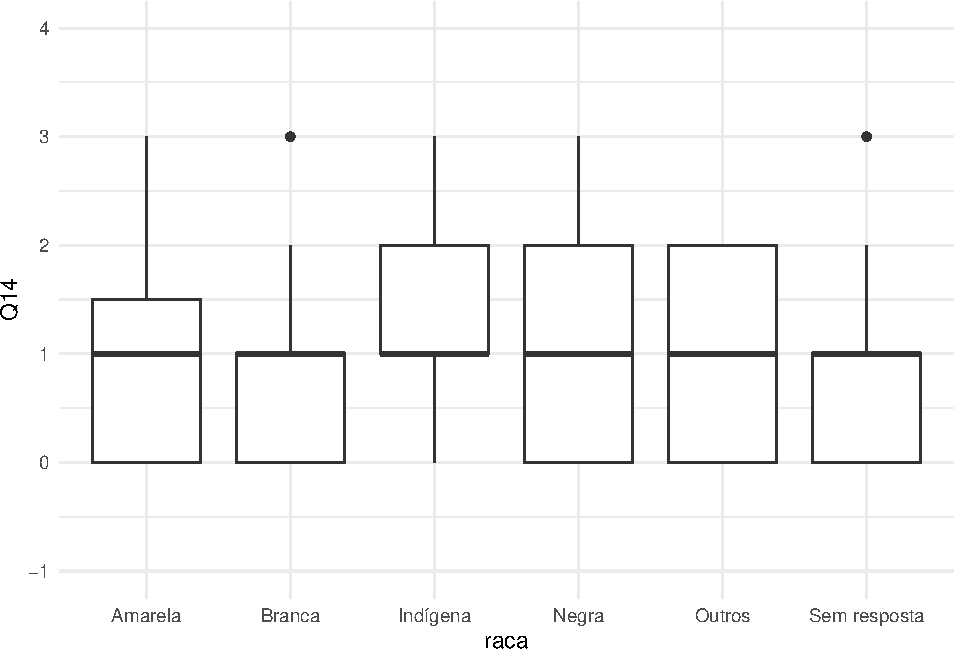
\includegraphics[width=0.75\linewidth]{relatorio_covid19_files/figure-latex/unnamed-chunk-48-1} \end{center}

\hypertarget{teste-de-kruskal-wallis-de-q14-por-rauxe7a}{%
\paragraph{Teste de Kruskal-Wallis de Q14 por Raça}\label{teste-de-kruskal-wallis-de-q14-por-rauxe7a}}

Como o valor-p é menor que 0.01 (nível de significância), rejeitamos a hipótese nula e as medianas de Q14 entre raças não são todas iguais.

\begin{longtable}[]{@{}ccc@{}}
\caption{\label{tab:unnamed-chunk-50}Valores-p para comparação múltipla de medianas: Q14 e Raça.}\tabularnewline
\toprule
Estatística & Parâmetro & valor p\tabularnewline
\midrule
\endfirsthead
\toprule
Estatística & Parâmetro & valor p\tabularnewline
\midrule
\endhead
31,43 & 5 & 0\tabularnewline
\bottomrule
\end{longtable}

\hypertarget{teste-de-nemeyi-de-q14-por-rauxe7a}{%
\paragraph{Teste de Nemeyi de Q14 por Raça}\label{teste-de-nemeyi-de-q14-por-rauxe7a}}

Existem valores-p menores que 0.01 (nível de significância), e para estes pares rejeitamos a hipótese nula e as medianas de Q14 entre estes pares de raças são diferentes.

\begin{longtable}[]{@{}lccccc@{}}
\caption{\label{tab:unnamed-chunk-52}Valores-p para o teste de Nemeyi de Q14 por Raça.}\tabularnewline
\toprule
& Amarela & Branca & Indígena & Negra & Outros\tabularnewline
\midrule
\endfirsthead
\toprule
& Amarela & Branca & Indígena & Negra & Outros\tabularnewline
\midrule
\endhead
Branca & 0,91 & & & &\tabularnewline
Indígena & 0,99 & 0,39 & & &\tabularnewline
Negra & 0,99 & 0,00 & 1,00 & &\tabularnewline
Outros & 1,00 & 0,99 & 0,95 & 0,94 &\tabularnewline
Sem resposta & 0,89 & 1,00 & 0,48 & 0,15 & 0,99\tabularnewline
\bottomrule
\end{longtable}

\cleardoublepage

\hypertarget{tabela-de-continguxeancia-tipo-de-escola-e-q14}{%
\paragraph{Tabela de contingência: Tipo de escola e Q14}\label{tabela-de-continguxeancia-tipo-de-escola-e-q14}}

Apenas sete crianças não estavam matriculadas na escola, e foram retiradas da análise para facilitar a análise de \emph{tipo de escola}.

\begin{longtable}[]{@{}ccccc@{}}
\caption{\label{tab:unnamed-chunk-53}Tabela de contingência: Tipo de escola e Q14.}\tabularnewline
\toprule
\begin{minipage}[b]{0.16\columnwidth}\centering
Tipo de Escola\strut
\end{minipage} & \begin{minipage}[b]{0.19\columnwidth}\centering
Muita preocupação\strut
\end{minipage} & \begin{minipage}[b]{0.19\columnwidth}\centering
Pouca preocupação\strut
\end{minipage} & \begin{minipage}[b]{0.17\columnwidth}\centering
Sem preocupação\strut
\end{minipage} & \begin{minipage}[b]{0.14\columnwidth}\centering
Sem resposta\strut
\end{minipage}\tabularnewline
\midrule
\endfirsthead
\toprule
\begin{minipage}[b]{0.16\columnwidth}\centering
Tipo de Escola\strut
\end{minipage} & \begin{minipage}[b]{0.19\columnwidth}\centering
Muita preocupação\strut
\end{minipage} & \begin{minipage}[b]{0.19\columnwidth}\centering
Pouca preocupação\strut
\end{minipage} & \begin{minipage}[b]{0.17\columnwidth}\centering
Sem preocupação\strut
\end{minipage} & \begin{minipage}[b]{0.14\columnwidth}\centering
Sem resposta\strut
\end{minipage}\tabularnewline
\midrule
\endhead
\begin{minipage}[t]{0.16\columnwidth}\centering
Particular\strut
\end{minipage} & \begin{minipage}[t]{0.19\columnwidth}\centering
94\strut
\end{minipage} & \begin{minipage}[t]{0.19\columnwidth}\centering
238\strut
\end{minipage} & \begin{minipage}[t]{0.17\columnwidth}\centering
238\strut
\end{minipage} & \begin{minipage}[t]{0.14\columnwidth}\centering
20\strut
\end{minipage}\tabularnewline
\begin{minipage}[t]{0.16\columnwidth}\centering
Pública\strut
\end{minipage} & \begin{minipage}[t]{0.19\columnwidth}\centering
171\strut
\end{minipage} & \begin{minipage}[t]{0.19\columnwidth}\centering
185\strut
\end{minipage} & \begin{minipage}[t]{0.17\columnwidth}\centering
85\strut
\end{minipage} & \begin{minipage}[t]{0.14\columnwidth}\centering
12\strut
\end{minipage}\tabularnewline
\bottomrule
\end{longtable}

\hypertarget{gruxe1fico-de-barras-tipo-de-escola-e-q14}{%
\paragraph{Gráfico de barras: Tipo de escola e Q14}\label{gruxe1fico-de-barras-tipo-de-escola-e-q14}}

Apenas sete crianças não estavam matriculadas na escola, e foram retiradas da análise para facilitar a análise de \emph{tipo de escola}.

\begin{center}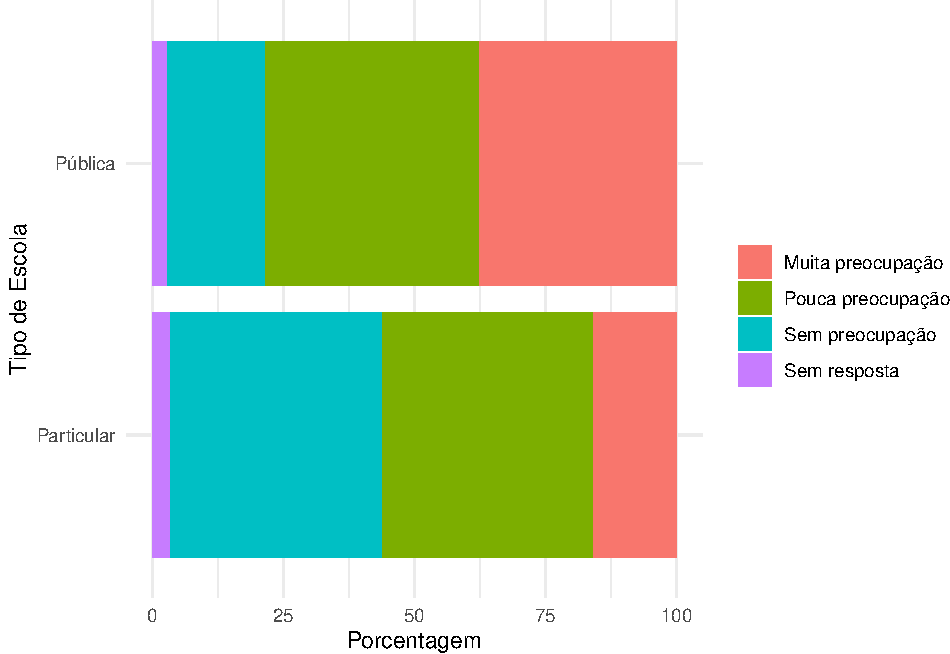
\includegraphics[width=0.75\linewidth]{relatorio_covid19_files/figure-latex/unnamed-chunk-54-1} \end{center}

\hypertarget{teste-qui-quadrado-6}{%
\paragraph{Teste qui-quadrado}\label{teste-qui-quadrado-6}}

Apenas sete crianças não estavam matriculadas na escola, e foram retiradas da análise para facilitar a análise de \emph{tipo de escola}.

Como o valor-p é menor que 0.01 (nível de significância), rejeitamos a hipótese nula e temos evidência estatística que as duas variáveis estão associadas.

\begin{longtable}[]{@{}ccc@{}}
\caption{\label{tab:unnamed-chunk-56}Teste qui-quadrado entre Escola e Q14.}\tabularnewline
\toprule
Estatística & Graus de liberdade & Valor-p\tabularnewline
\midrule
\endfirsthead
\toprule
Estatística & Graus de liberdade & Valor-p\tabularnewline
\midrule
\endhead
86,99 & 3 & 0\tabularnewline
\bottomrule
\end{longtable}

\cleardoublepage

\hypertarget{medidas-de-resumo-q14-por-tipo-de-escola}{%
\paragraph{Medidas de Resumo Q14 por Tipo de escola}\label{medidas-de-resumo-q14-por-tipo-de-escola}}

Apenas sete crianças não estavam matriculadas na escola, e foram retiradas da análise para facilitar a análise de \emph{tipo de escola}.

\begin{longtable}[]{@{}cccccc@{}}
\caption{\label{tab:unnamed-chunk-57}Medidas de resumo de Q14 por Escola.}\tabularnewline
\toprule
Q14 & Média & Desvio Padrão & Mediana & 1 Quartil & 3 Quartil\tabularnewline
\midrule
\endfirsthead
\toprule
Q14 & Média & Desvio Padrão & Mediana & 1 Quartil & 3 Quartil\tabularnewline
\midrule
\endhead
Particular & 0,82 & 0,82 & 1 & 0 & 1\tabularnewline
Pública & 1,24 & 0,78 & 1 & 1 & 2\tabularnewline
\bottomrule
\end{longtable}

\hypertarget{boxplot-de-q14-por-tipo-de-escola}{%
\paragraph{Boxplot de Q14 por Tipo de escola}\label{boxplot-de-q14-por-tipo-de-escola}}

Apenas sete crianças não estavam matriculadas na escola, e foram retiradas da análise para facilitar a análise de \emph{tipo de escola}.

\begin{center}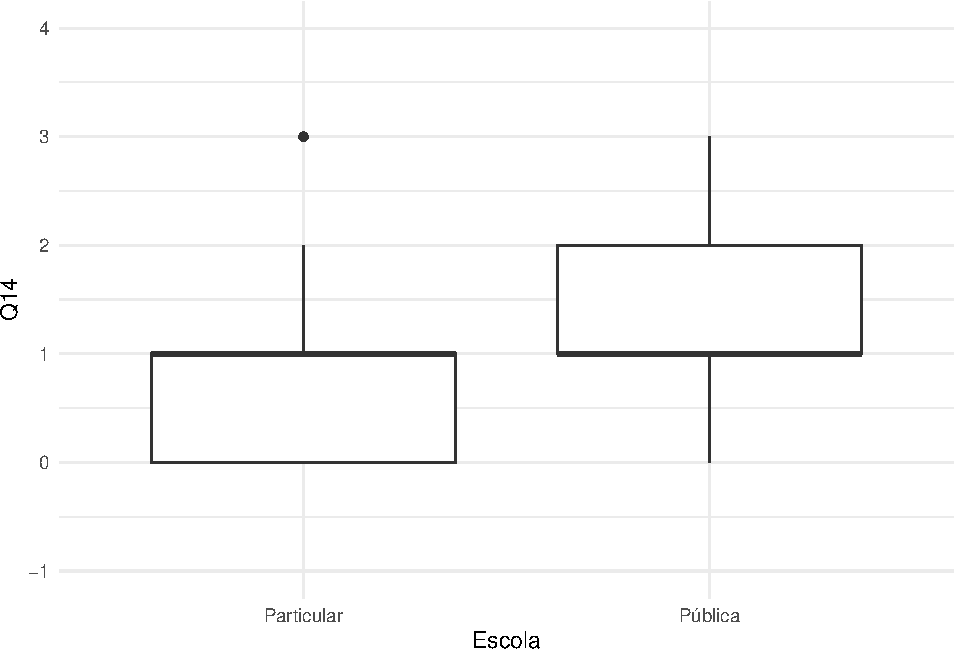
\includegraphics[width=0.75\linewidth]{relatorio_covid19_files/figure-latex/unnamed-chunk-58-1} \end{center}

\hypertarget{teste-de-kruskal-wallis-de-q14-por-tipo-de-escola}{%
\paragraph{Teste de Kruskal-Wallis de Q14 por Tipo de escola}\label{teste-de-kruskal-wallis-de-q14-por-tipo-de-escola}}

Apenas sete crianças não estavam matriculadas na escola, e foram retiradas da análise para facilitar a análise de \emph{tipo de escola}.

Como o valor-p é menor que 0.01 (nível de significância), rejeitamos a hipótese nula e as medianas de Q14 entre tipos de escola são diferentes.

\begin{longtable}[]{@{}ccc@{}}
\caption{\label{tab:unnamed-chunk-60}Valores-p para comparação múltipla de medianas: Q14 e Tipo de escola.}\tabularnewline
\toprule
Estatística & Parâmetro & valor p\tabularnewline
\midrule
\endfirsthead
\toprule
Estatística & Parâmetro & valor p\tabularnewline
\midrule
\endhead
73,42 & 1 & 0\tabularnewline
\bottomrule
\end{longtable}

\hypertarget{teste-de-nemeyi-de-q14-por-tipo-de-escola}{%
\paragraph{Teste de Nemeyi de Q14 por Tipo de escola}\label{teste-de-nemeyi-de-q14-por-tipo-de-escola}}

Apenas sete crianças não estavam matriculadas na escola, e foram retiradas da análise para facilitar a análise de \emph{tipo de escola}.

O valor-p é maior ou igual que 0.01 (nível de significância), e rejeitamos a hipótese nula e as medianas de Q14 entre tipos de escolas são diferentes.

\begin{longtable}[]{@{}lc@{}}
\caption{\label{tab:unnamed-chunk-62}Teste de Nemeyi de Q14 por Escola.}\tabularnewline
\toprule
& Particular\tabularnewline
\midrule
\endfirsthead
\toprule
& Particular\tabularnewline
\midrule
\endhead
Pública & 0\tabularnewline
\bottomrule
\end{longtable}

\cleardoublepage

\hypertarget{q15}{%
\subsection{Q15}\label{q15}}

A variável Q15 corresponde ao campo de númeo 13 com enunciado \textbf{O quanto você está preocupado hoje com as questões abaixo} no quesito:

\begin{itemize}
\tightlist
\item
  \emph{Que falte comida nos supermercados}
\end{itemize}

\hypertarget{anuxe1lise-descritiva-para-q15}{%
\subsubsection{Análise descritiva para Q15}\label{anuxe1lise-descritiva-para-q15}}

\hypertarget{gruxe1fico-de-barras-q15}{%
\paragraph{Gráfico de barras: Q15}\label{gruxe1fico-de-barras-q15}}

\begin{center}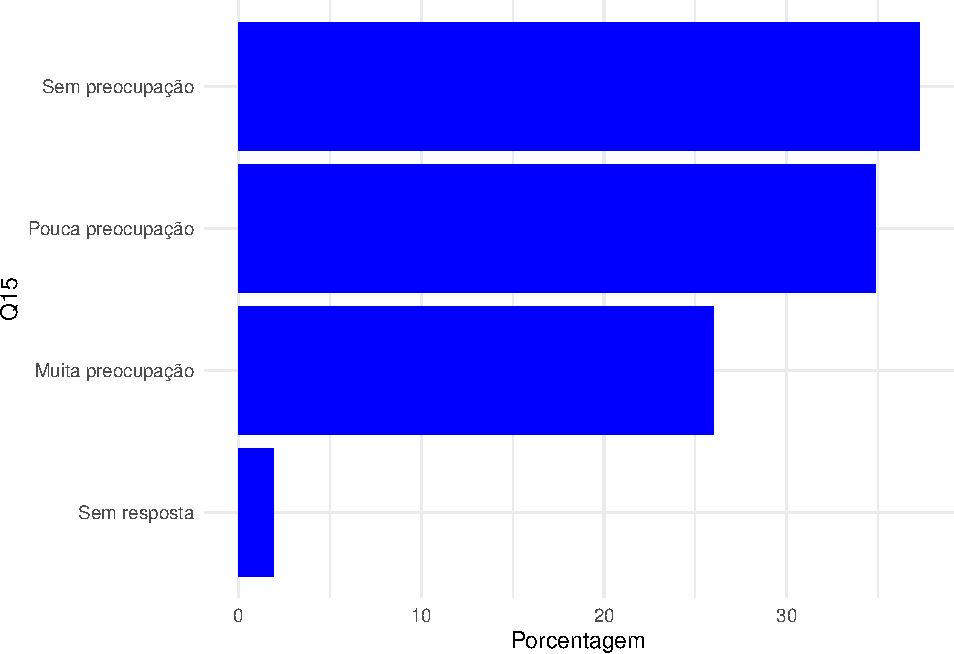
\includegraphics[width=0.75\linewidth]{relatorio_covid19_files/figure-latex/unnamed-chunk-69-1} \end{center}

\hypertarget{tabela-de-distribuiuxe7uxe3o-q15}{%
\paragraph{Tabela de distribuição: Q15}\label{tabela-de-distribuiuxe7uxe3o-q15}}

\begin{longtable}[]{@{}cccc@{}}
\caption{\label{tab:unnamed-chunk-70}Que falte comida nos supermercados}\tabularnewline
\toprule
Q15 & Frequência & Frequência relativa & Porcentagem\tabularnewline
\midrule
\endfirsthead
\toprule
Q15 & Frequência & Frequência relativa & Porcentagem\tabularnewline
\midrule
\endhead
Sem preocupação & 391 & 0,37 & 37,24\tabularnewline
Pouca preocupação & 366 & 0,35 & 34,86\tabularnewline
Muita preocupação & 273 & 0,26 & 26,00\tabularnewline
Sem resposta & 20 & 0,02 & 1,90\tabularnewline
\bottomrule
\end{longtable}

\hypertarget{medidas-de-resumo-q15}{%
\paragraph{Medidas de resumo: Q15}\label{medidas-de-resumo-q15}}

\begin{longtable}[]{@{}ccccc@{}}
\caption{\label{tab:unnamed-chunk-71}Resumos para variável Q15.}\tabularnewline
\toprule
Média & Desvio Padrão & Mediana & 1Qua & 3Qua\tabularnewline
\midrule
\endfirsthead
\toprule
Média & Desvio Padrão & Mediana & 1Qua & 3Qua\tabularnewline
\midrule
\endhead
0,93 & 0,84 & 1 & 0 & 2\tabularnewline
\bottomrule
\end{longtable}

\cleardoublepage

\hypertarget{anuxe1lise-bidimensional-q15}{%
\subsubsection{Análise bidimensional Q15}\label{anuxe1lise-bidimensional-q15}}

\hypertarget{tabela-de-continguxeancia-cidade-e-q15}{%
\paragraph{Tabela de contingência: Cidade e Q15}\label{tabela-de-continguxeancia-cidade-e-q15}}

\begin{longtable}[]{@{}ccccc@{}}
\caption{\label{tab:unnamed-chunk-72}Tabela de contingência: Cidade e Q15.}\tabularnewline
\toprule
Cidade & Muita preocupação & Pouca preocupação & Sem preocupação & Sem resposta\tabularnewline
\midrule
\endfirsthead
\toprule
Cidade & Muita preocupação & Pouca preocupação & Sem preocupação & Sem resposta\tabularnewline
\midrule
\endhead
Camaçari & 72 & 77 & 40 & 8\tabularnewline
Candeias & 12 & 15 & 9 & 2\tabularnewline
Lauro de Freitas & 11 & 26 & 23 & 1\tabularnewline
Outros & 23 & 41 & 19 &\tabularnewline
Pojuca & 25 & 27 & 10 & 2\tabularnewline
Salvador & 113 & 225 & 217 & 18\tabularnewline
Simões Filho & 9 & 17 & 7 & 1\tabularnewline
\bottomrule
\end{longtable}

\hypertarget{gruxe1fico-de-barras-cidade-e-q15}{%
\paragraph{Gráfico de barras: Cidade e Q15}\label{gruxe1fico-de-barras-cidade-e-q15}}

\begin{center}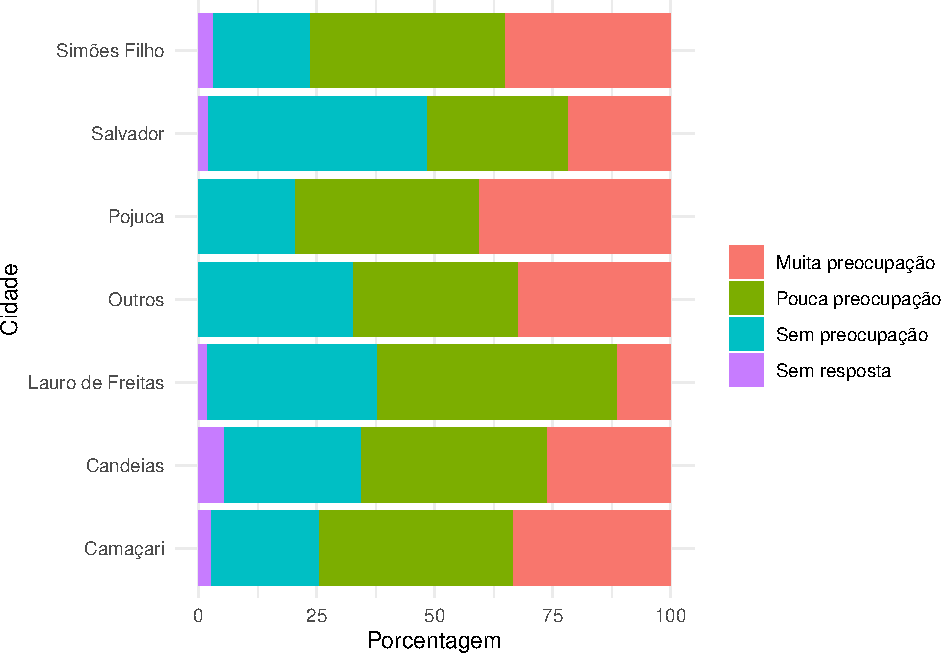
\includegraphics[width=0.75\linewidth]{relatorio_covid19_files/figure-latex/unnamed-chunk-73-1} \end{center}

\hypertarget{teste-qui-quadrado-7}{%
\paragraph{Teste qui-quadrado}\label{teste-qui-quadrado-7}}

Como o valor-p é menor que 0.01 (nível de significância), rejeitamos a hipótese nula e temos evidência estatística que as duas variáveis estão associadas.

\begin{longtable}[]{@{}ccc@{}}
\caption{\label{tab:unnamed-chunk-75}Teste qui-quadrado entre Cidade e Q15.}\tabularnewline
\toprule
Estatística & Graus de liberdade & Valor-p\tabularnewline
\midrule
\endfirsthead
\toprule
Estatística & Graus de liberdade & Valor-p\tabularnewline
\midrule
\endhead
70,88 & 18 & 0\tabularnewline
\bottomrule
\end{longtable}

\cleardoublepage

\hypertarget{medidas-de-resumo-q15-por-cidade}{%
\paragraph{Medidas de Resumo Q15 por Cidade}\label{medidas-de-resumo-q15-por-cidade}}

\begin{longtable}[]{@{}cccccc@{}}
\caption{\label{tab:unnamed-chunk-76}Medidas de resumo de Q15 por Cidade.}\tabularnewline
\toprule
Q15 & Média & Desvio Padrão & Mediana & 1 Quartil & 3 Quartil\tabularnewline
\midrule
\endfirsthead
\toprule
Q15 & Média & Desvio Padrão & Mediana & 1 Quartil & 3 Quartil\tabularnewline
\midrule
\endhead
Camaçari & 1,16 & 0,80 & 1 & 1 & 2\tabularnewline
Candeias & 1,08 & 0,88 & 1 & 0 & 2\tabularnewline
Lauro de Freitas & 0,79 & 0,71 & 1 & 0 & 1\tabularnewline
Outros & 1,00 & 0,81 & 1 & 0 & 2\tabularnewline
Pojuca & 1,20 & 0,76 & 1 & 1 & 2\tabularnewline
Salvador & 0,79 & 0,85 & 1 & 0 & 1\tabularnewline
Simões Filho & 1,21 & 0,81 & 1 & 1 & 2\tabularnewline
\bottomrule
\end{longtable}

\hypertarget{boxplot-de-q15-por-cidade}{%
\paragraph{Boxplot de Q15 por Cidade}\label{boxplot-de-q15-por-cidade}}

\begin{center}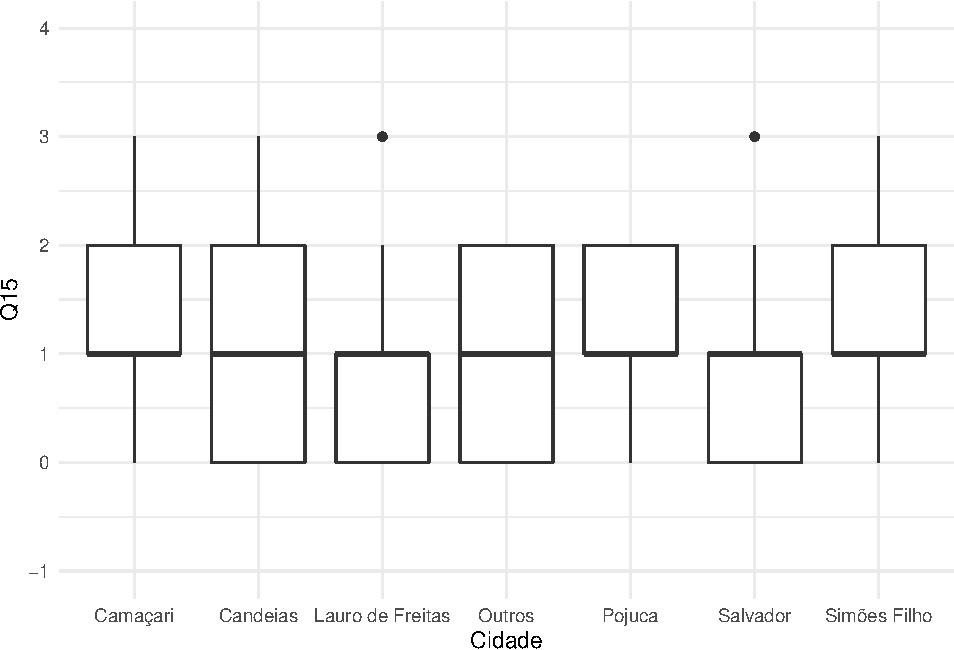
\includegraphics[width=0.75\linewidth]{relatorio_covid19_files/figure-latex/unnamed-chunk-77-1} \end{center}

\hypertarget{teste-de-kruskal-wallis-de-q15-por-cidade}{%
\paragraph{Teste de Kruskal-Wallis de Q15 por Cidade}\label{teste-de-kruskal-wallis-de-q15-por-cidade}}

Como o valor-p é menor que 0.01 (nível de significância), rejeitamos a hipótese nula e as medianas de Q15 entre as crianças de diversas cidades não são todas iguais.

\begin{longtable}[]{@{}ccc@{}}
\caption{\label{tab:unnamed-chunk-79}Valor-p para o teste de Kruskal-Wallis: Q15 e Cidade.}\tabularnewline
\toprule
Estatística & Parâmetro & valor p\tabularnewline
\midrule
\endfirsthead
\toprule
Estatística & Parâmetro & valor p\tabularnewline
\midrule
\endhead
47,65 & 6 & 0\tabularnewline
\bottomrule
\end{longtable}

\hypertarget{teste-de-nemeyi-de-q15-por-cidade}{%
\paragraph{Teste de Nemeyi de Q15 por Cidade}\label{teste-de-nemeyi-de-q15-por-cidade}}

Existem valores-p menores que 0.01 (nível de significância), e para estes pares rejeitamos a hipótese nula e as medianas de Q15 entre as crianças destes pares de cidades são diferentes.

\begin{longtable}[]{@{}lcccccc@{}}
\caption{\label{tab:unnamed-chunk-81}Valores-p para o teste de comparação múltipla de Nemeyi de Q15 por Cidade.}\tabularnewline
\toprule
& Camaçari & Candeias & Lauro de Freitas & Outros & Pojuca & Salvador\tabularnewline
\midrule
\endfirsthead
\toprule
& Camaçari & Candeias & Lauro de Freitas & Outros & Pojuca & Salvador\tabularnewline
\midrule
\endhead
Candeias & 1,00 & & & & &\tabularnewline
Lauro de Freitas & 0,07 & 0,77 & & & &\tabularnewline
Outros & 0,85 & 1,00 & 0,79 & & &\tabularnewline
Pojuca & 1,00 & 0,98 & 0,10 & 0,79 & &\tabularnewline
Salvador & 0,00 & 0,49 & 1,00 & 0,30 & 0 &\tabularnewline
Simões Filho & 1,00 & 0,99 & 0,31 & 0,93 & 1 & 0,09\tabularnewline
\bottomrule
\end{longtable}

\cleardoublepage

\hypertarget{tabela-de-continguxeancia-guxeanero-e-q15}{%
\paragraph{Tabela de contingência: Gênero e Q15}\label{tabela-de-continguxeancia-guxeanero-e-q15}}

Apenas seis crianças se identificaram com o gênero \emph{outros} e foram removidas na análise estatística.

\begin{longtable}[]{@{}ccccc@{}}
\caption{\label{tab:unnamed-chunk-82}Tabela de contingência: Gênero e Q15.}\tabularnewline
\toprule
Gênero & Muita preocupação & Pouca preocupação & Sem preocupação & Sem resposta\tabularnewline
\midrule
\endfirsthead
\toprule
Gênero & Muita preocupação & Pouca preocupação & Sem preocupação & Sem resposta\tabularnewline
\midrule
\endhead
Menina & 147 & 183 & 200 & 11\tabularnewline
Menino & 126 & 180 & 188 & 9\tabularnewline
\bottomrule
\end{longtable}

\hypertarget{gruxe1fico-de-barras-guxeanero-e-q15}{%
\paragraph{Gráfico de barras: Gênero e Q15}\label{gruxe1fico-de-barras-guxeanero-e-q15}}

Apenas seis crianças se identificaram com o gênero \emph{outros} e foram removidas na análise estatística.

\begin{center}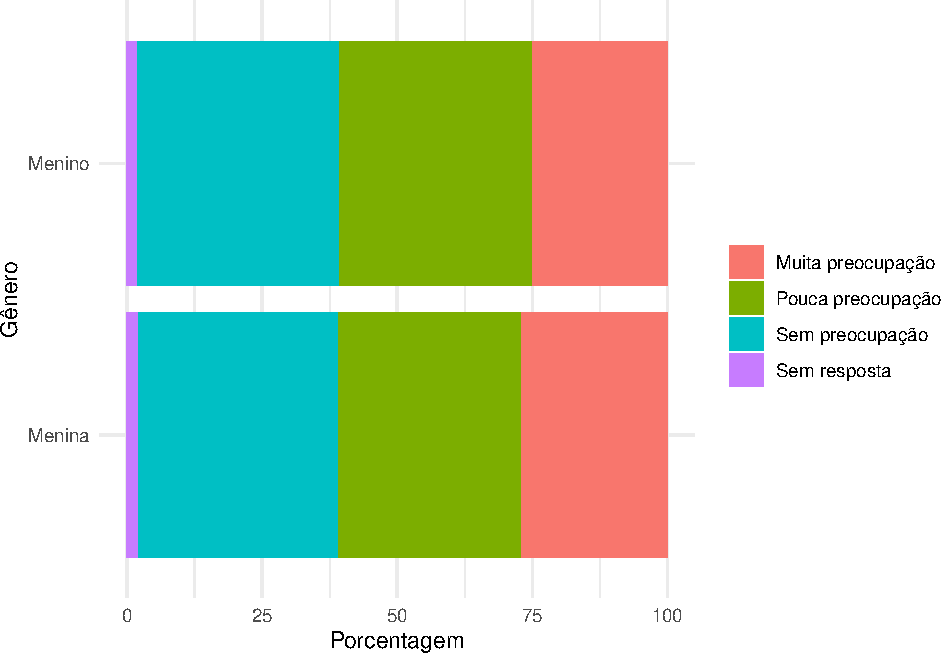
\includegraphics[width=0.75\linewidth]{relatorio_covid19_files/figure-latex/unnamed-chunk-83-1} \end{center}

\hypertarget{teste-qui-quadrado-8}{%
\paragraph{Teste qui-quadrado}\label{teste-qui-quadrado-8}}

Apenas seis crianças se identificaram com o gênero \emph{outros} e foram removidas na análise estatística.

Como o valor-p é igual ou maior que 0.01 (nível de significância), não rejeitamos a hipótese nula e não temos evidência estatística que as duas variáveis estão associadas.

\begin{longtable}[]{@{}ccc@{}}
\caption{\label{tab:unnamed-chunk-85}Teste qui-quadrado entre Gênero e Q15.}\tabularnewline
\toprule
Estatística & Graus de liberdade & Valor-p\tabularnewline
\midrule
\endfirsthead
\toprule
Estatística & Graus de liberdade & Valor-p\tabularnewline
\midrule
\endhead
0,83 & 3 & 0,84\tabularnewline
\bottomrule
\end{longtable}

\cleardoublepage

\hypertarget{medidas-de-resumo-q15-por-guxeanero}{%
\paragraph{Medidas de Resumo Q15 por Gênero}\label{medidas-de-resumo-q15-por-guxeanero}}

Apenas seis crianças se identificaram com o gênero \emph{outros} e foram removidas na análise estatística.

\begin{longtable}[]{@{}cccccc@{}}
\caption{\label{tab:unnamed-chunk-86}Medidas de resumo de Q15 por Gênero.}\tabularnewline
\toprule
Q15 & Média & Desvio Padrão & Mediana & 1 Quartil & 3 Quartil\tabularnewline
\midrule
\endfirsthead
\toprule
Q15 & Média & Desvio Padrão & Mediana & 1 Quartil & 3 Quartil\tabularnewline
\midrule
\endhead
Menina & 0,94 & 0,85 & 1 & 0 & 2\tabularnewline
Menino & 0,91 & 0,83 & 1 & 0 & 2\tabularnewline
\bottomrule
\end{longtable}

\hypertarget{boxplot-de-q15-por-guxeanero}{%
\paragraph{Boxplot de Q15 por Gênero}\label{boxplot-de-q15-por-guxeanero}}

Apenas seis crianças se identificaram com o gênero \emph{outros} e foram removidas na análise estatística.

\begin{center}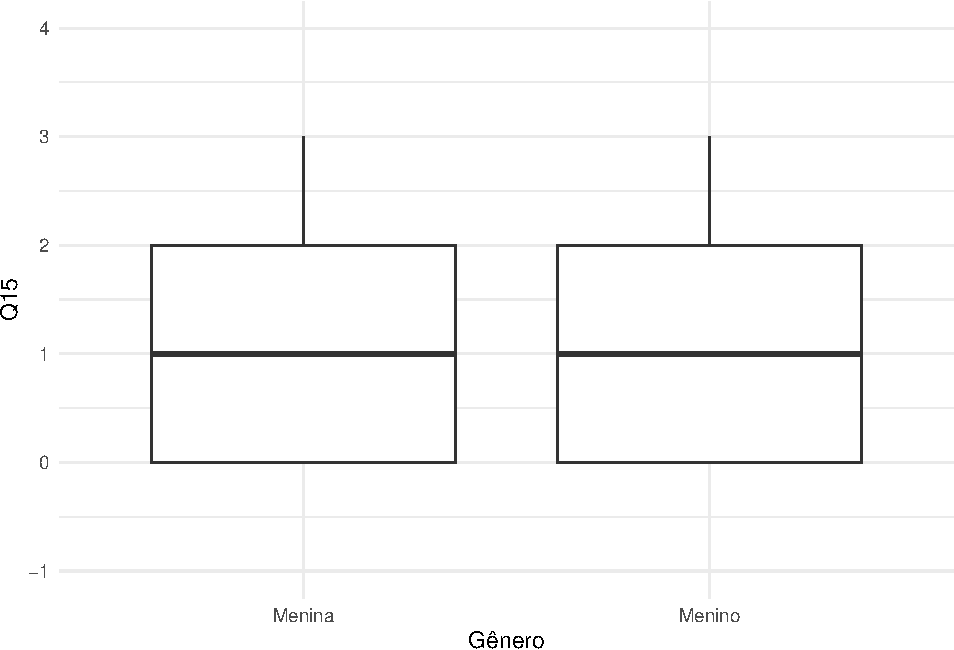
\includegraphics[width=0.75\linewidth]{relatorio_covid19_files/figure-latex/unnamed-chunk-87-1} \end{center}

\hypertarget{teste-de-kruskal-wallis-de-q15-por-guxeanero}{%
\paragraph{Teste de Kruskal-Wallis de Q15 por Gênero}\label{teste-de-kruskal-wallis-de-q15-por-guxeanero}}

Apenas seis crianças se identificaram com o gênero \emph{outros} e foram removidas na análise estatística.

Como o valor-p é maior ou igual a 0.01 (nível de significância), não rejeitamos a hipótese nula e as medianas de Q15 entre meninos e meninas são iguais.

\begin{longtable}[]{@{}ccc@{}}
\caption{\label{tab:unnamed-chunk-89}Valores-p para comparação múltipla de medianas: Q15 e Gênero.}\tabularnewline
\toprule
Estatística & Parâmetro & valor p\tabularnewline
\midrule
\endfirsthead
\toprule
Estatística & Parâmetro & valor p\tabularnewline
\midrule
\endhead
0,29 & 1 & 0,59\tabularnewline
\bottomrule
\end{longtable}

\hypertarget{teste-de-nemeyi-de-q15-por-guxeanero}{%
\paragraph{Teste de Nemeyi de Q15 por Gênero}\label{teste-de-nemeyi-de-q15-por-guxeanero}}

Apenas seis crianças se identificaram com o gênero \emph{outros} e foram removidas na análise estatística.

Como os valores-p são iguais ou maiores que 0.01 (nível de significância), não rejeitamos a hipótese nula e as medianas de Q15 entre meninos e meninas são iguais.

\begin{longtable}[]{@{}lc@{}}
\caption{\label{tab:unnamed-chunk-91}valores-p para o teste de comparação múltipla de Nemeyi de Q15 por Gênero.}\tabularnewline
\toprule
& Menina\tabularnewline
\midrule
\endfirsthead
\toprule
& Menina\tabularnewline
\midrule
\endhead
Menino & 0,61\tabularnewline
\bottomrule
\end{longtable}

\cleardoublepage

\hypertarget{tabela-de-continguxeancia-idade-e-q15}{%
\paragraph{Tabela de contingência: Idade e Q15}\label{tabela-de-continguxeancia-idade-e-q15}}

\begin{longtable}[]{@{}ccccc@{}}
\caption{\label{tab:unnamed-chunk-92}Tabela de contingência: Idade e Q15.}\tabularnewline
\toprule
Idade & Muita preocupação & Pouca preocupação & Sem preocupação & Sem resposta\tabularnewline
\midrule
\endfirsthead
\toprule
Idade & Muita preocupação & Pouca preocupação & Sem preocupação & Sem resposta\tabularnewline
\midrule
\endhead
8 & 58 & 70 & 64 & 3\tabularnewline
9 & 53 & 62 & 69 & 2\tabularnewline
10 & 72 & 90 & 81 & 7\tabularnewline
11 & 51 & 89 & 97 & 3\tabularnewline
12 & 39 & 55 & 80 & 5\tabularnewline
\bottomrule
\end{longtable}

\hypertarget{gruxe1fico-de-barras-idade-e-q15}{%
\paragraph{Gráfico de barras: Idade e Q15}\label{gruxe1fico-de-barras-idade-e-q15}}

\begin{center}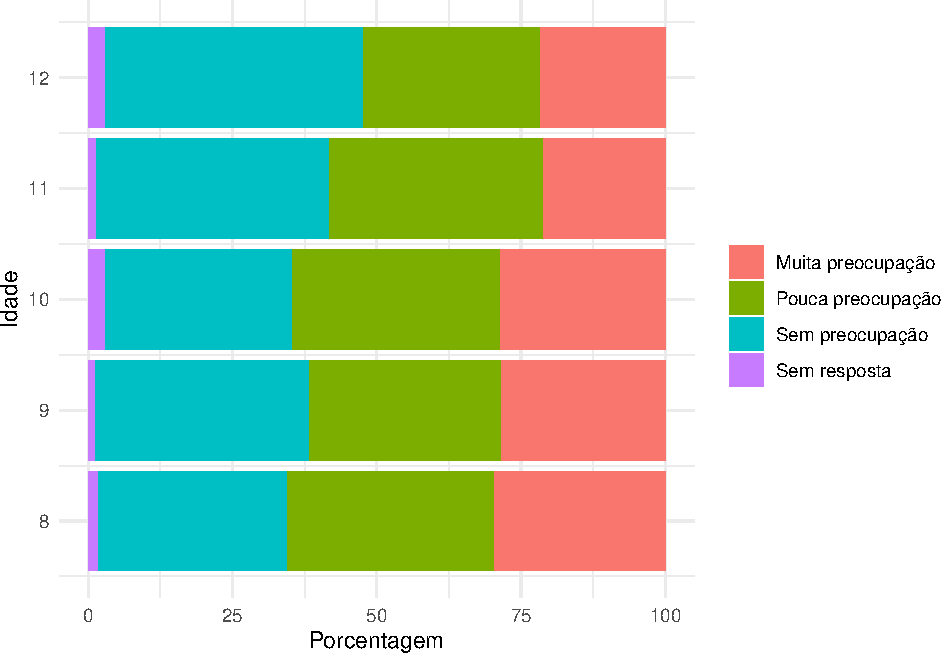
\includegraphics[width=0.75\linewidth]{relatorio_covid19_files/figure-latex/unnamed-chunk-93-1} \end{center}

\hypertarget{teste-qui-quadrado-9}{%
\paragraph{Teste qui-quadrado}\label{teste-qui-quadrado-9}}

Como o valor-p é igual ou maior que 0.01 (nível de significância), não rejeitamos a hipótese nula e não temos evidência estatística que as duas variáveis estão associadas.

\begin{longtable}[]{@{}ccc@{}}
\caption{\label{tab:unnamed-chunk-95}Teste qui-quadrado entre Idade e Q15.}\tabularnewline
\toprule
Estatística & Graus de liberdade & Valor-p\tabularnewline
\midrule
\endfirsthead
\toprule
Estatística & Graus de liberdade & Valor-p\tabularnewline
\midrule
\endhead
16,11 & 12 & 0,19\tabularnewline
\bottomrule
\end{longtable}

\cleardoublepage

\hypertarget{medidas-de-resumo-q15-por-idade}{%
\paragraph{Medidas de Resumo Q15 por Idade}\label{medidas-de-resumo-q15-por-idade}}

\begin{longtable}[]{@{}cccccc@{}}
\caption{\label{tab:unnamed-chunk-96}Medidas de resumo de Q15 por Idade.}\tabularnewline
\toprule
Q15 & Média & Desvio Padrão & Mediana & 1 Quartil & 3 Quartil\tabularnewline
\midrule
\endfirsthead
\toprule
Q15 & Média & Desvio Padrão & Mediana & 1 Quartil & 3 Quartil\tabularnewline
\midrule
\endhead
8 & 1,00 & 0,83 & 1 & 0 & 2\tabularnewline
9 & 0,94 & 0,84 & 1 & 0 & 2\tabularnewline
10 & 1,02 & 0,85 & 1 & 0 & 2\tabularnewline
11 & 0,83 & 0,80 & 1 & 0 & 1\tabularnewline
12 & 0,83 & 0,87 & 1 & 0 & 1\tabularnewline
\bottomrule
\end{longtable}

\hypertarget{boxplot-de-q15-por-idade}{%
\paragraph{Boxplot de Q15 por Idade}\label{boxplot-de-q15-por-idade}}

\begin{center}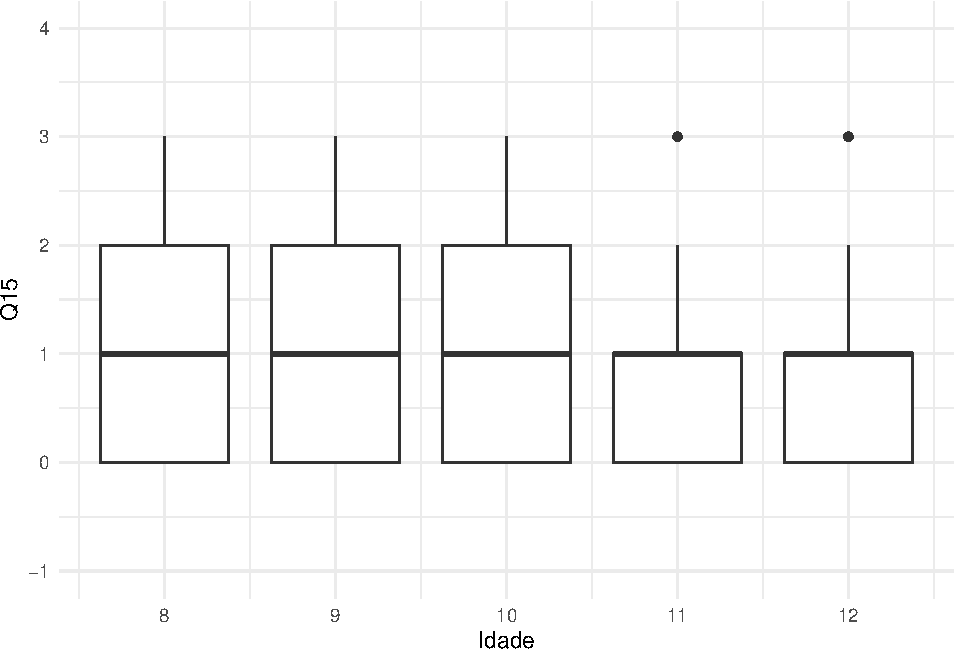
\includegraphics[width=0.75\linewidth]{relatorio_covid19_files/figure-latex/unnamed-chunk-97-1} \end{center}

\hypertarget{teste-de-kruskal-wallis-de-q15-por-idade}{%
\paragraph{Teste de Kruskal-Wallis de Q15 por Idade}\label{teste-de-kruskal-wallis-de-q15-por-idade}}

Como o valor-p é maior ou igual a 0.01 (nível de significância), não rejeitamos a hipótese nula e as medianas de Q15 entre as idades são iguais.

\begin{longtable}[]{@{}ccc@{}}
\caption{\label{tab:unnamed-chunk-99}Valores-p para comparação múltipla de medianas: Q15 e Idade.}\tabularnewline
\toprule
Estatística & Parâmetro & valor p\tabularnewline
\midrule
\endfirsthead
\toprule
Estatística & Parâmetro & valor p\tabularnewline
\midrule
\endhead
10,58 & 4 & 0,03\tabularnewline
\bottomrule
\end{longtable}

\hypertarget{teste-de-nemeyi-de-q15-por-idade}{%
\paragraph{Teste de Nemeyi de Q15 por Idade}\label{teste-de-nemeyi-de-q15-por-idade}}

Como os valores-p são iguais ou maiores que 0.01 (nível de significância), não rejeitamos a hipótese nula e as medianas de Q15 entre pares de crianças de diferentes idades são todas iguais.

\begin{longtable}[]{@{}lcccc@{}}
\caption{\label{tab:unnamed-chunk-101}Teste de Nemeyi de Q15 por Idade.}\tabularnewline
\toprule
& 8 & 9 & 10 & 11\tabularnewline
\midrule
\endfirsthead
\toprule
& 8 & 9 & 10 & 11\tabularnewline
\midrule
\endhead
9 & 0,95 & & &\tabularnewline
10 & 1,00 & 0,89 & &\tabularnewline
11 & 0,29 & 0,76 & 0,16 &\tabularnewline
12 & 0,24 & 0,67 & 0,14 & 1\tabularnewline
\bottomrule
\end{longtable}

\cleardoublepage

\hypertarget{tabela-de-continguxeancia-rauxe7a-e-q15}{%
\paragraph{Tabela de contingência: Raça e Q15}\label{tabela-de-continguxeancia-rauxe7a-e-q15}}

\begin{longtable}[]{@{}ccccc@{}}
\caption{\label{tab:unnamed-chunk-102}Tabela de contingência: Raça e Q15.}\tabularnewline
\toprule
Raça & Muita preocupação & Pouca preocupação & Sem preocupação & Sem resposta\tabularnewline
\midrule
\endfirsthead
\toprule
Raça & Muita preocupação & Pouca preocupação & Sem preocupação & Sem resposta\tabularnewline
\midrule
\endhead
Amarela & 3 & 9 & 5 & 2\tabularnewline
Branca & 36 & 59 & 116 & 2\tabularnewline
Indígena & 6 & 10 & 5 &\tabularnewline
Negra & 219 & 276 & 239 & 15\tabularnewline
Outros & 4 & 3 & 8 & 1\tabularnewline
Sem resposta & 5 & 9 & 18 &\tabularnewline
\bottomrule
\end{longtable}

\hypertarget{gruxe1fico-de-barras-rauxe7a-e-q15}{%
\paragraph{Gráfico de barras: Raça e Q15}\label{gruxe1fico-de-barras-rauxe7a-e-q15}}

\begin{center}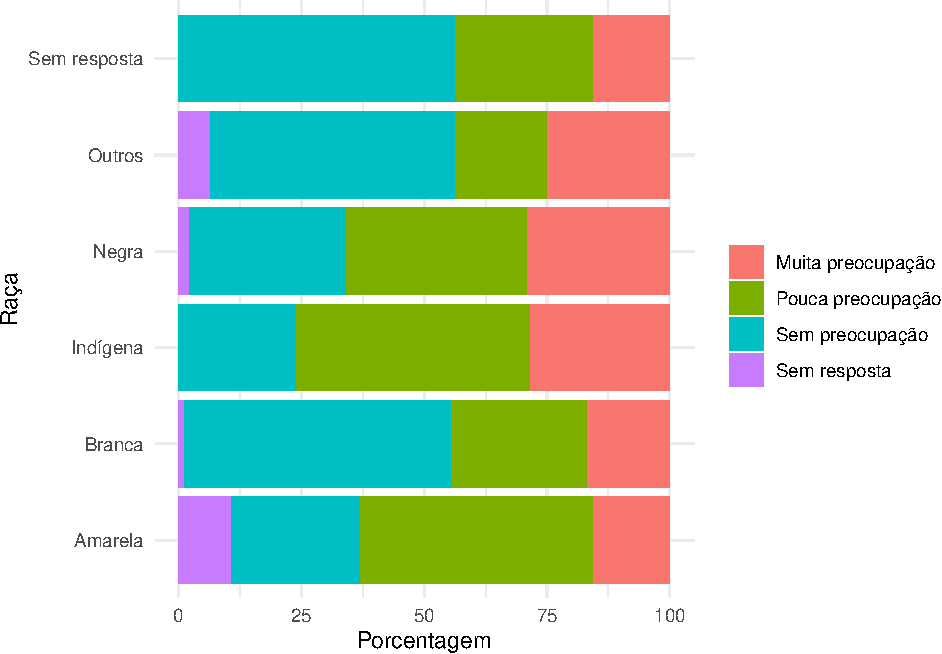
\includegraphics[width=0.75\linewidth]{relatorio_covid19_files/figure-latex/unnamed-chunk-103-1} \end{center}

\hypertarget{teste-qui-quadrado-10}{%
\paragraph{Teste qui-quadrado}\label{teste-qui-quadrado-10}}

Como o valor-p é menor que 0.01 (nível de significância), rejeitamos a hipótese nula e temos evidência estatística que as duas variáveis estão associadas.

\begin{longtable}[]{@{}ccc@{}}
\caption{\label{tab:unnamed-chunk-105}Teste qui-quadrado entre raca e Q15.}\tabularnewline
\toprule
Estatística & Graus de liberdade & Valor-p\tabularnewline
\midrule
\endfirsthead
\toprule
Estatística & Graus de liberdade & Valor-p\tabularnewline
\midrule
\endhead
58,57 & 15 & 0\tabularnewline
\bottomrule
\end{longtable}

\cleardoublepage

\hypertarget{medidas-de-resumo-q15-por-rauxe7a}{%
\paragraph{Medidas de Resumo Q15 por Raça}\label{medidas-de-resumo-q15-por-rauxe7a}}

\begin{longtable}[]{@{}cccccc@{}}
\caption{\label{tab:unnamed-chunk-106}Medidas de resumo de Q15 por raca.}\tabularnewline
\toprule
Q15 & Média & Desvio Padrão & Mediana & 1 Quartil & 3 Quartil\tabularnewline
\midrule
\endfirsthead
\toprule
Q15 & Média & Desvio Padrão & Mediana & 1 Quartil & 3 Quartil\tabularnewline
\midrule
\endhead
Amarela & 1,11 & 0,94 & 1,0 & 0,5 & 1,5\tabularnewline
Branca & 0,64 & 0,79 & 0,0 & 0,0 & 1,0\tabularnewline
Indígena & 1,05 & 0,74 & 1,0 & 1,0 & 2,0\tabularnewline
Negra & 1,01 & 0,83 & 1,0 & 0,0 & 2,0\tabularnewline
Outros & 0,88 & 1,02 & 0,5 & 0,0 & 2,0\tabularnewline
Sem resposta & 0,59 & 0,76 & 0,0 & 0,0 & 1,0\tabularnewline
\bottomrule
\end{longtable}

\hypertarget{boxplot-de-q15-por-rauxe7a}{%
\paragraph{Boxplot de Q15 por Raça}\label{boxplot-de-q15-por-rauxe7a}}

\begin{center}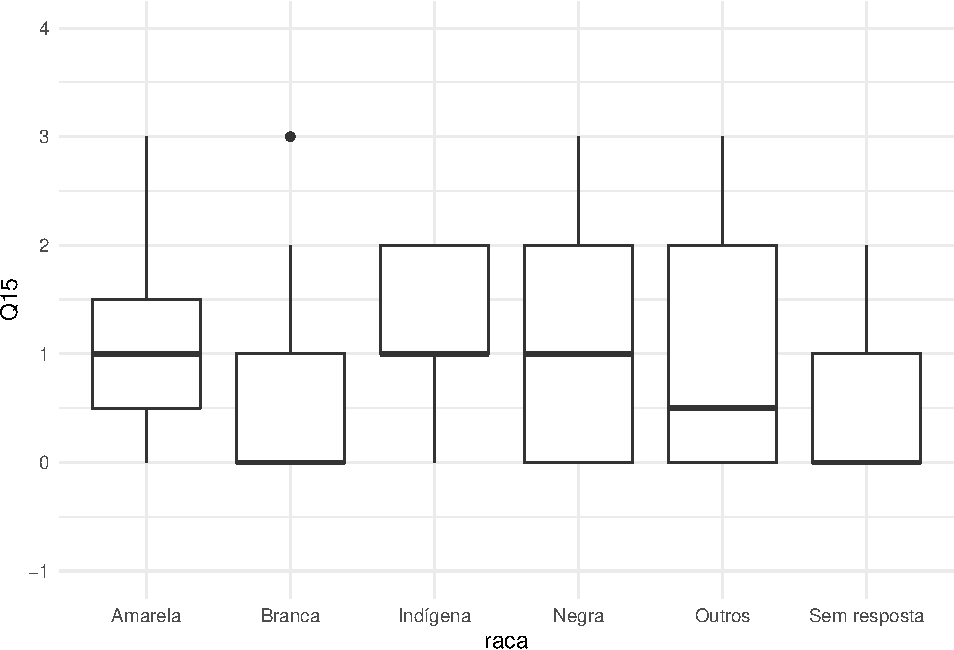
\includegraphics[width=0.75\linewidth]{relatorio_covid19_files/figure-latex/unnamed-chunk-107-1} \end{center}

\hypertarget{teste-de-kruskal-wallis-de-q15-por-rauxe7a}{%
\paragraph{Teste de Kruskal-Wallis de Q15 por Raça}\label{teste-de-kruskal-wallis-de-q15-por-rauxe7a}}

Como o valor-p é menor que 0.01 (nível de significância), rejeitamos a hipótese nula e as medianas de Q15 entre raças não são todas iguais.

\begin{longtable}[]{@{}ccc@{}}
\caption{\label{tab:unnamed-chunk-109}Valores-p para comparação múltipla de medianas: Q15 e Raça.}\tabularnewline
\toprule
Estatística & Parâmetro & valor p\tabularnewline
\midrule
\endfirsthead
\toprule
Estatística & Parâmetro & valor p\tabularnewline
\midrule
\endhead
40,7 & 5 & 0\tabularnewline
\bottomrule
\end{longtable}

\hypertarget{teste-de-nemeyi-de-q15-por-rauxe7a}{%
\paragraph{Teste de Nemeyi de Q15 por Raça}\label{teste-de-nemeyi-de-q15-por-rauxe7a}}

Existem valores-p menores que 0.01 (nível de significância), e para estes pares rejeitamos a hipótese nula e as medianas de Q15 entre estes pares de raças são diferentes.

\begin{longtable}[]{@{}lccccc@{}}
\caption{\label{tab:unnamed-chunk-111}Valores-p para o teste de Nemeyi de Q15 por Raça.}\tabularnewline
\toprule
& Amarela & Branca & Indígena & Negra & Outros\tabularnewline
\midrule
\endfirsthead
\toprule
& Amarela & Branca & Indígena & Negra & Outros\tabularnewline
\midrule
\endhead
Branca & 0,32 & & & &\tabularnewline
Indígena & 1,00 & 0,26 & & &\tabularnewline
Negra & 1,00 & 0,00 & 1,00 & &\tabularnewline
Outros & 0,97 & 0,96 & 0,97 & 0,97 &\tabularnewline
Sem resposta & 0,43 & 1,00 & 0,39 & 0,09 & 0,95\tabularnewline
\bottomrule
\end{longtable}

\cleardoublepage

\hypertarget{tabela-de-continguxeancia-tipo-de-escola-e-q15}{%
\paragraph{Tabela de contingência: Tipo de escola e Q15}\label{tabela-de-continguxeancia-tipo-de-escola-e-q15}}

Apenas sete crianças não estavam matriculadas na escola, e foram retiradas da análise para facilitar a análise de \emph{tipo de escola}.

\begin{longtable}[]{@{}ccccc@{}}
\caption{\label{tab:unnamed-chunk-112}Tabela de contingência: Tipo de escola e Q15.}\tabularnewline
\toprule
\begin{minipage}[b]{0.16\columnwidth}\centering
Tipo de Escola\strut
\end{minipage} & \begin{minipage}[b]{0.19\columnwidth}\centering
Muita preocupação\strut
\end{minipage} & \begin{minipage}[b]{0.19\columnwidth}\centering
Pouca preocupação\strut
\end{minipage} & \begin{minipage}[b]{0.17\columnwidth}\centering
Sem preocupação\strut
\end{minipage} & \begin{minipage}[b]{0.14\columnwidth}\centering
Sem resposta\strut
\end{minipage}\tabularnewline
\midrule
\endfirsthead
\toprule
\begin{minipage}[b]{0.16\columnwidth}\centering
Tipo de Escola\strut
\end{minipage} & \begin{minipage}[b]{0.19\columnwidth}\centering
Muita preocupação\strut
\end{minipage} & \begin{minipage}[b]{0.19\columnwidth}\centering
Pouca preocupação\strut
\end{minipage} & \begin{minipage}[b]{0.17\columnwidth}\centering
Sem preocupação\strut
\end{minipage} & \begin{minipage}[b]{0.14\columnwidth}\centering
Sem resposta\strut
\end{minipage}\tabularnewline
\midrule
\endhead
\begin{minipage}[t]{0.16\columnwidth}\centering
Particular\strut
\end{minipage} & \begin{minipage}[t]{0.19\columnwidth}\centering
107\strut
\end{minipage} & \begin{minipage}[t]{0.19\columnwidth}\centering
174\strut
\end{minipage} & \begin{minipage}[t]{0.17\columnwidth}\centering
297\strut
\end{minipage} & \begin{minipage}[t]{0.14\columnwidth}\centering
12\strut
\end{minipage}\tabularnewline
\begin{minipage}[t]{0.16\columnwidth}\centering
Pública\strut
\end{minipage} & \begin{minipage}[t]{0.19\columnwidth}\centering
166\strut
\end{minipage} & \begin{minipage}[t]{0.19\columnwidth}\centering
189\strut
\end{minipage} & \begin{minipage}[t]{0.17\columnwidth}\centering
90\strut
\end{minipage} & \begin{minipage}[t]{0.14\columnwidth}\centering
8\strut
\end{minipage}\tabularnewline
\bottomrule
\end{longtable}

\hypertarget{gruxe1fico-de-barras-tipo-de-escola-e-q15}{%
\paragraph{Gráfico de barras: Tipo de escola e Q15}\label{gruxe1fico-de-barras-tipo-de-escola-e-q15}}

Apenas sete crianças não estavam matriculadas na escola, e foram retiradas da análise para facilitar a análise de \emph{tipo de escola}.

\begin{center}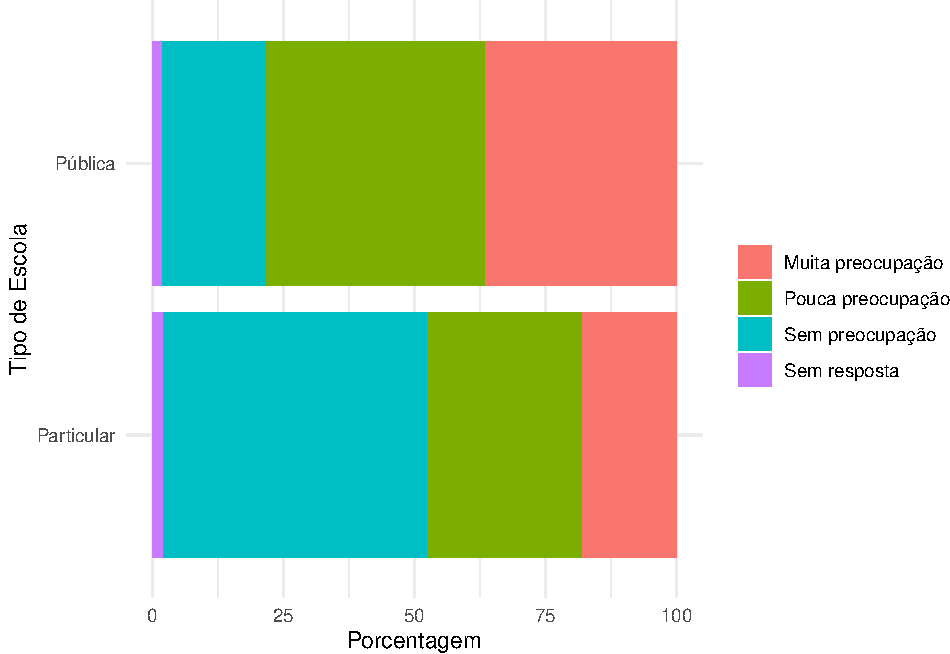
\includegraphics[width=0.75\linewidth]{relatorio_covid19_files/figure-latex/unnamed-chunk-113-1} \end{center}

\hypertarget{teste-qui-quadrado-11}{%
\paragraph{Teste qui-quadrado}\label{teste-qui-quadrado-11}}

Apenas sete crianças não estavam matriculadas na escola, e foram retiradas da análise para facilitar a análise de \emph{tipo de escola}.

Como o valor-p é menor que 0.01 (nível de significância), rejeitamos a hipótese nula e temos evidência estatística que as duas variáveis estão associadas.

\begin{longtable}[]{@{}ccc@{}}
\caption{\label{tab:unnamed-chunk-115}Teste qui-quadrado entre Escola e Q15.}\tabularnewline
\toprule
Estatística & Graus de liberdade & Valor-p\tabularnewline
\midrule
\endfirsthead
\toprule
Estatística & Graus de liberdade & Valor-p\tabularnewline
\midrule
\endhead
108,77 & 3 & 0\tabularnewline
\bottomrule
\end{longtable}

\cleardoublepage

\hypertarget{medidas-de-resumo-q15-por-tipo-de-escola}{%
\paragraph{Medidas de Resumo Q15 por Tipo de escola}\label{medidas-de-resumo-q15-por-tipo-de-escola}}

Apenas sete crianças não estavam matriculadas na escola, e foram retiradas da análise para facilitar a análise de \emph{tipo de escola}.

\begin{longtable}[]{@{}cccccc@{}}
\caption{\label{tab:unnamed-chunk-116}Medidas de resumo de Q15 por Escola.}\tabularnewline
\toprule
Q15 & Média & Desvio Padrão & Mediana & 1 Quartil & 3 Quartil\tabularnewline
\midrule
\endfirsthead
\toprule
Q15 & Média & Desvio Padrão & Mediana & 1 Quartil & 3 Quartil\tabularnewline
\midrule
\endhead
Particular & 0,72 & 0,83 & 0 & 0 & 1\tabularnewline
Pública & 1,20 & 0,77 & 1 & 1 & 2\tabularnewline
\bottomrule
\end{longtable}

\hypertarget{boxplot-de-q15-por-tipo-de-escola}{%
\paragraph{Boxplot de Q15 por Tipo de escola}\label{boxplot-de-q15-por-tipo-de-escola}}

Apenas sete crianças não estavam matriculadas na escola, e foram retiradas da análise para facilitar a análise de \emph{tipo de escola}.

\begin{center}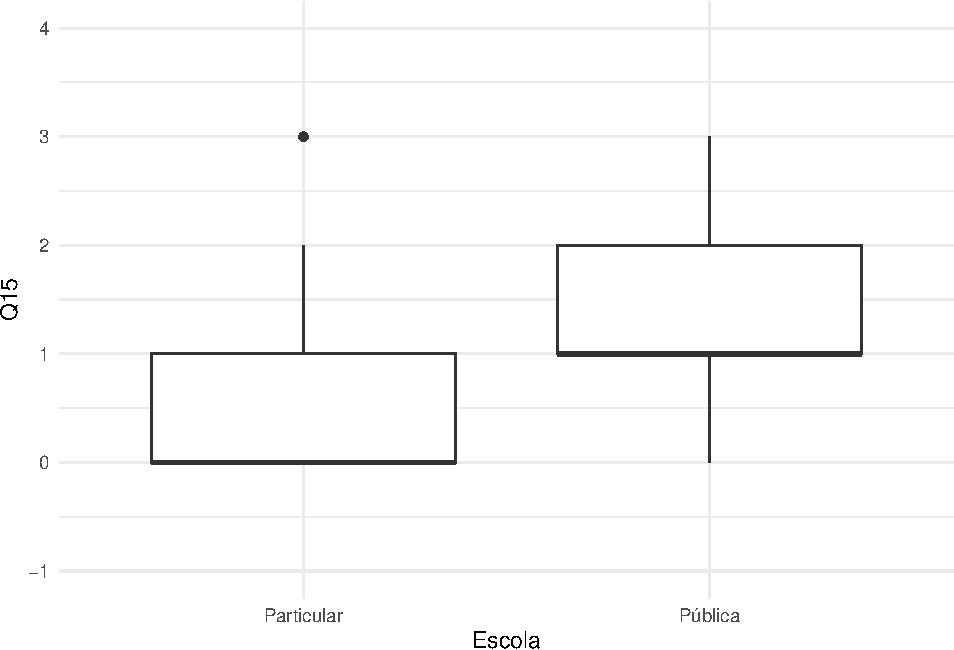
\includegraphics[width=0.75\linewidth]{relatorio_covid19_files/figure-latex/unnamed-chunk-117-1} \end{center}

\hypertarget{teste-de-kruskal-wallis-de-q15-por-tipo-de-escola}{%
\paragraph{Teste de Kruskal-Wallis de Q15 por Tipo de escola}\label{teste-de-kruskal-wallis-de-q15-por-tipo-de-escola}}

Apenas sete crianças não estavam matriculadas na escola, e foram retiradas da análise para facilitar a análise de \emph{tipo de escola}.

Como o valor-p é menor que 0.01 (nível de significância), rejeitamos a hipótese nula e as medianas de Q15 entre tipos de escola são diferentes.

\begin{longtable}[]{@{}ccc@{}}
\caption{\label{tab:unnamed-chunk-119}Valores-p para comparação múltipla de medianas: Q15 e Tipo de escola.}\tabularnewline
\toprule
Estatística & Parâmetro & valor p\tabularnewline
\midrule
\endfirsthead
\toprule
Estatística & Parâmetro & valor p\tabularnewline
\midrule
\endhead
93,87 & 1 & 0\tabularnewline
\bottomrule
\end{longtable}

\hypertarget{teste-de-nemeyi-de-q15-por-tipo-de-escola}{%
\paragraph{Teste de Nemeyi de Q15 por Tipo de escola}\label{teste-de-nemeyi-de-q15-por-tipo-de-escola}}

Apenas sete crianças não estavam matriculadas na escola, e foram retiradas da análise para facilitar a análise de \emph{tipo de escola}.

O valor-p é maior ou igual que 0.01 (nível de significância), e rejeitamos a hipótese nula e as medianas de Q15 entre tipos de escolas são diferentes.

\begin{longtable}[]{@{}lc@{}}
\caption{\label{tab:unnamed-chunk-121}Teste de Nemeyi de Q15 por Escola.}\tabularnewline
\toprule
& Particular\tabularnewline
\midrule
\endfirsthead
\toprule
& Particular\tabularnewline
\midrule
\endhead
Pública & 0\tabularnewline
\bottomrule
\end{longtable}

\cleardoublepage

\hypertarget{q16}{%
\subsection{Q16}\label{q16}}

A variável Q16 corresponde ao campo de númeo 13 com enunciado \textbf{O quanto você está preocupado hoje com as questões abaixo} no quesito:

\begin{itemize}
\tightlist
\item
  \emph{Que falte comida na minha casa}
\end{itemize}

\hypertarget{anuxe1lise-descritiva-para-q16}{%
\subsubsection{Análise descritiva para Q16}\label{anuxe1lise-descritiva-para-q16}}

\hypertarget{gruxe1fico-de-barras-q16}{%
\paragraph{Gráfico de barras: Q16}\label{gruxe1fico-de-barras-q16}}

\begin{center}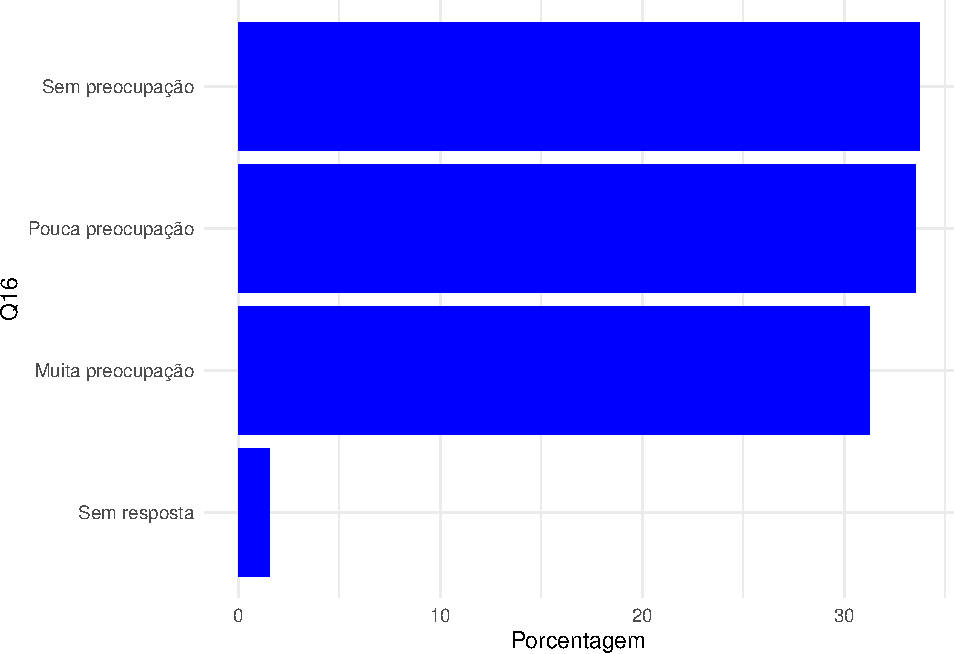
\includegraphics[width=0.75\linewidth]{relatorio_covid19_files/figure-latex/unnamed-chunk-128-1} \end{center}

\hypertarget{tabela-de-distribuiuxe7uxe3o-q16}{%
\paragraph{Tabela de distribuição: Q16}\label{tabela-de-distribuiuxe7uxe3o-q16}}

\begin{longtable}[]{@{}cccc@{}}
\caption{\label{tab:unnamed-chunk-129}Que falte comida na minha casa}\tabularnewline
\toprule
Q16 & Frequência & Frequência relativa & Porcentagem\tabularnewline
\midrule
\endfirsthead
\toprule
Q16 & Frequência & Frequência relativa & Porcentagem\tabularnewline
\midrule
\endhead
Sem preocupação & 354 & 0,34 & 33,71\tabularnewline
Pouca preocupação & 352 & 0,34 & 33,52\tabularnewline
Muita preocupação & 328 & 0,31 & 31,24\tabularnewline
Sem resposta & 16 & 0,02 & 1,52\tabularnewline
\bottomrule
\end{longtable}

\hypertarget{medidas-de-resumo-q16}{%
\paragraph{Medidas de resumo: Q16}\label{medidas-de-resumo-q16}}

\begin{longtable}[]{@{}ccccc@{}}
\caption{\label{tab:unnamed-chunk-130}Resumos para variável Q16.}\tabularnewline
\toprule
Média & Desvio Padrão & Mediana & 1Qua & 3Qua\tabularnewline
\midrule
\endfirsthead
\toprule
Média & Desvio Padrão & Mediana & 1Qua & 3Qua\tabularnewline
\midrule
\endhead
1,01 & 0,84 & 1 & 0 & 2\tabularnewline
\bottomrule
\end{longtable}

\cleardoublepage

\hypertarget{anuxe1lise-bidimensional-q16}{%
\subsubsection{Análise bidimensional Q16}\label{anuxe1lise-bidimensional-q16}}

\hypertarget{tabela-de-continguxeancia-cidade-e-q16}{%
\paragraph{Tabela de contingência: Cidade e Q16}\label{tabela-de-continguxeancia-cidade-e-q16}}

\begin{longtable}[]{@{}ccccc@{}}
\caption{\label{tab:unnamed-chunk-131}Tabela de contingência: Cidade e Q16.}\tabularnewline
\toprule
Cidade & Muita preocupação & Pouca preocupação & Sem preocupação & Sem resposta\tabularnewline
\midrule
\endfirsthead
\toprule
Cidade & Muita preocupação & Pouca preocupação & Sem preocupação & Sem resposta\tabularnewline
\midrule
\endhead
Camaçari & 72 & 77 & 40 & 8\tabularnewline
Candeias & 12 & 15 & 9 & 2\tabularnewline
Lauro de Freitas & 11 & 26 & 23 & 1\tabularnewline
Outros & 23 & 41 & 19 &\tabularnewline
Pojuca & 25 & 27 & 10 & 2\tabularnewline
Salvador & 113 & 225 & 217 & 18\tabularnewline
Simões Filho & 9 & 17 & 7 & 1\tabularnewline
\bottomrule
\end{longtable}

\hypertarget{gruxe1fico-de-barras-cidade-e-q16}{%
\paragraph{Gráfico de barras: Cidade e Q16}\label{gruxe1fico-de-barras-cidade-e-q16}}

\begin{center}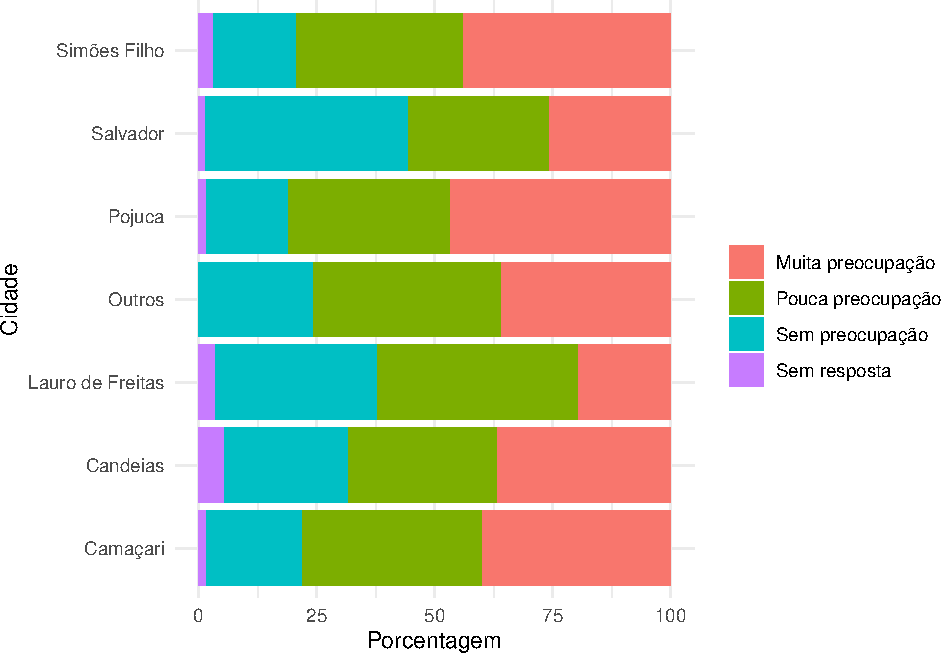
\includegraphics[width=0.75\linewidth]{relatorio_covid19_files/figure-latex/unnamed-chunk-132-1} \end{center}

\hypertarget{teste-qui-quadrado-12}{%
\paragraph{Teste qui-quadrado}\label{teste-qui-quadrado-12}}

Como o valor-p é menor que 0.01 (nível de significância), rejeitamos a hipótese nula e temos evidência estatística que as duas variáveis estão associadas.

\begin{longtable}[]{@{}ccc@{}}
\caption{\label{tab:unnamed-chunk-134}Teste qui-quadrado entre Cidade e Q16.}\tabularnewline
\toprule
Estatística & Graus de liberdade & Valor-p\tabularnewline
\midrule
\endfirsthead
\toprule
Estatística & Graus de liberdade & Valor-p\tabularnewline
\midrule
\endhead
69,06 & 18 & 0\tabularnewline
\bottomrule
\end{longtable}

\cleardoublepage

\hypertarget{medidas-de-resumo-q16-por-cidade}{%
\paragraph{Medidas de Resumo Q16 por Cidade}\label{medidas-de-resumo-q16-por-cidade}}

\begin{longtable}[]{@{}cccccc@{}}
\caption{\label{tab:unnamed-chunk-135}Medidas de resumo de Q16 por Cidade.}\tabularnewline
\toprule
Q16 & Média & Desvio Padrão & Mediana & 1 Quartil & 3 Quartil\tabularnewline
\midrule
\endfirsthead
\toprule
Q16 & Média & Desvio Padrão & Mediana & 1 Quartil & 3 Quartil\tabularnewline
\midrule
\endhead
Camaçari & 1,23 & 0,78 & 1 & 1,00 & 2\tabularnewline
Candeias & 1,21 & 0,91 & 1 & 0,25 & 2\tabularnewline
Lauro de Freitas & 0,92 & 0,82 & 1 & 0,00 & 1\tabularnewline
Outros & 1,12 & 0,77 & 1 & 1,00 & 2\tabularnewline
Pojuca & 1,33 & 0,78 & 1 & 1,00 & 2\tabularnewline
Salvador & 0,85 & 0,85 & 1 & 0,00 & 2\tabularnewline
Simões Filho & 1,32 & 0,81 & 1 & 1,00 & 2\tabularnewline
\bottomrule
\end{longtable}

\hypertarget{boxplot-de-q16-por-cidade}{%
\paragraph{Boxplot de Q16 por Cidade}\label{boxplot-de-q16-por-cidade}}

\begin{center}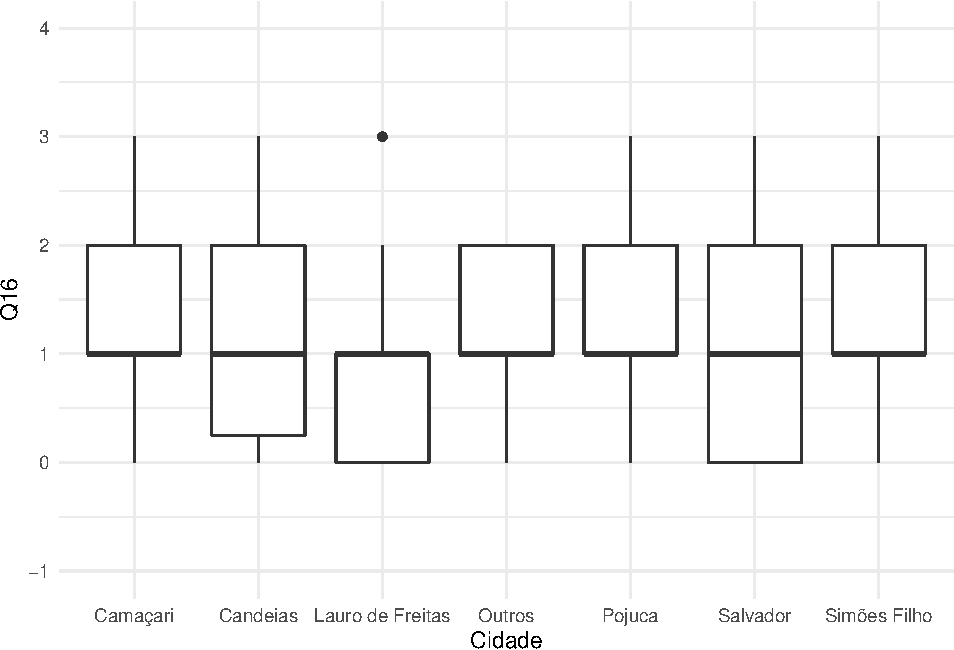
\includegraphics[width=0.75\linewidth]{relatorio_covid19_files/figure-latex/unnamed-chunk-136-1} \end{center}

\hypertarget{teste-de-kruskal-wallis-de-q16-por-cidade}{%
\paragraph{Teste de Kruskal-Wallis de Q16 por Cidade}\label{teste-de-kruskal-wallis-de-q16-por-cidade}}

Como o valor-p é menor que 0.01 (nível de significância), rejeitamos a hipótese nula e as medianas de Q16 entre as crianças de diversas cidades não são todas iguais.

\begin{longtable}[]{@{}ccc@{}}
\caption{\label{tab:unnamed-chunk-138}Valor-p para o teste de Kruskal-Wallis: Q16 e Cidade.}\tabularnewline
\toprule
Estatística & Parâmetro & valor p\tabularnewline
\midrule
\endfirsthead
\toprule
Estatística & Parâmetro & valor p\tabularnewline
\midrule
\endhead
52,68 & 6 & 0\tabularnewline
\bottomrule
\end{longtable}

\hypertarget{teste-de-nemeyi-de-q16-por-cidade}{%
\paragraph{Teste de Nemeyi de Q16 por Cidade}\label{teste-de-nemeyi-de-q16-por-cidade}}

Existem valores-p menores que 0.01 (nível de significância), e para estes pares rejeitamos a hipótese nula e as medianas de Q16 entre as crianças destes pares de cidades são diferentes.

\begin{longtable}[]{@{}lcccccc@{}}
\caption{\label{tab:unnamed-chunk-140}Valores-p para o teste de comparação múltipla de Nemeyi de Q16 por Cidade.}\tabularnewline
\toprule
& Camaçari & Candeias & Lauro de Freitas & Outros & Pojuca & Salvador\tabularnewline
\midrule
\endfirsthead
\toprule
& Camaçari & Candeias & Lauro de Freitas & Outros & Pojuca & Salvador\tabularnewline
\midrule
\endhead
Candeias & 1,00 & & & & &\tabularnewline
Lauro de Freitas & 0,17 & 0,71 & & & &\tabularnewline
Outros & 0,98 & 1,00 & 0,76 & & &\tabularnewline
Pojuca & 0,99 & 0,99 & 0,11 & 0,82 & &\tabularnewline
Salvador & 0,00 & 0,24 & 1,00 & 0,10 & 0 &\tabularnewline
Simões Filho & 1,00 & 1,00 & 0,31 & 0,94 & 1 & 0,04\tabularnewline
\bottomrule
\end{longtable}

\cleardoublepage

\hypertarget{tabela-de-continguxeancia-guxeanero-e-q16}{%
\paragraph{Tabela de contingência: Gênero e Q16}\label{tabela-de-continguxeancia-guxeanero-e-q16}}

Apenas seis crianças se identificaram com o gênero \emph{outros} e foram removidas na análise estatística.

\begin{longtable}[]{@{}ccccc@{}}
\caption{\label{tab:unnamed-chunk-141}Tabela de contingência: Gênero e Q16.}\tabularnewline
\toprule
Gênero & Muita preocupação & Pouca preocupação & Sem preocupação & Sem resposta\tabularnewline
\midrule
\endfirsthead
\toprule
Gênero & Muita preocupação & Pouca preocupação & Sem preocupação & Sem resposta\tabularnewline
\midrule
\endhead
Menina & 167 & 178 & 186 & 10\tabularnewline
Menino & 160 & 172 & 165 & 6\tabularnewline
\bottomrule
\end{longtable}

\hypertarget{gruxe1fico-de-barras-guxeanero-e-q16}{%
\paragraph{Gráfico de barras: Gênero e Q16}\label{gruxe1fico-de-barras-guxeanero-e-q16}}

Apenas seis crianças se identificaram com o gênero \emph{outros} e foram removidas na análise estatística.

\begin{center}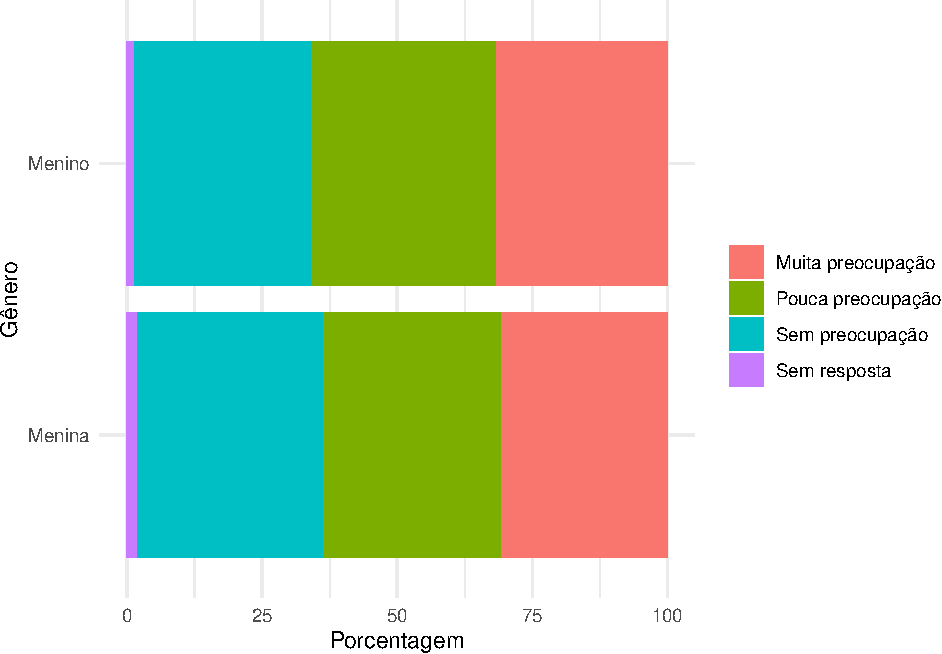
\includegraphics[width=0.75\linewidth]{relatorio_covid19_files/figure-latex/unnamed-chunk-142-1} \end{center}

\hypertarget{teste-qui-quadrado-13}{%
\paragraph{Teste qui-quadrado}\label{teste-qui-quadrado-13}}

Apenas seis crianças se identificaram com o gênero \emph{outros} e foram removidas na análise estatística.

Como o valor-p é igual ou maior que 0.01 (nível de significância), não rejeitamos a hipótese nula e não temos evidência estatística que as duas variáveis estão associadas.

\begin{longtable}[]{@{}ccc@{}}
\caption{\label{tab:unnamed-chunk-144}Teste qui-quadrado entre Gênero e Q16.}\tabularnewline
\toprule
Estatística & Graus de liberdade & Valor-p\tabularnewline
\midrule
\endfirsthead
\toprule
Estatística & Graus de liberdade & Valor-p\tabularnewline
\midrule
\endhead
1,13 & 3 & 0,77\tabularnewline
\bottomrule
\end{longtable}

\cleardoublepage

\hypertarget{medidas-de-resumo-q16-por-guxeanero}{%
\paragraph{Medidas de Resumo Q16 por Gênero}\label{medidas-de-resumo-q16-por-guxeanero}}

Apenas seis crianças se identificaram com o gênero \emph{outros} e foram removidas na análise estatística.

\begin{longtable}[]{@{}cccccc@{}}
\caption{\label{tab:unnamed-chunk-145}Medidas de resumo de Q16 por Gênero.}\tabularnewline
\toprule
Q16 & Média & Desvio Padrão & Mediana & 1 Quartil & 3 Quartil\tabularnewline
\midrule
\endfirsthead
\toprule
Q16 & Média & Desvio Padrão & Mediana & 1 Quartil & 3 Quartil\tabularnewline
\midrule
\endhead
Menina & 1,00 & 0,85 & 1 & 0 & 2\tabularnewline
Menino & 1,01 & 0,83 & 1 & 0 & 2\tabularnewline
\bottomrule
\end{longtable}

\hypertarget{boxplot-de-q16-por-guxeanero}{%
\paragraph{Boxplot de Q16 por Gênero}\label{boxplot-de-q16-por-guxeanero}}

Apenas seis crianças se identificaram com o gênero \emph{outros} e foram removidas na análise estatística.

\begin{center}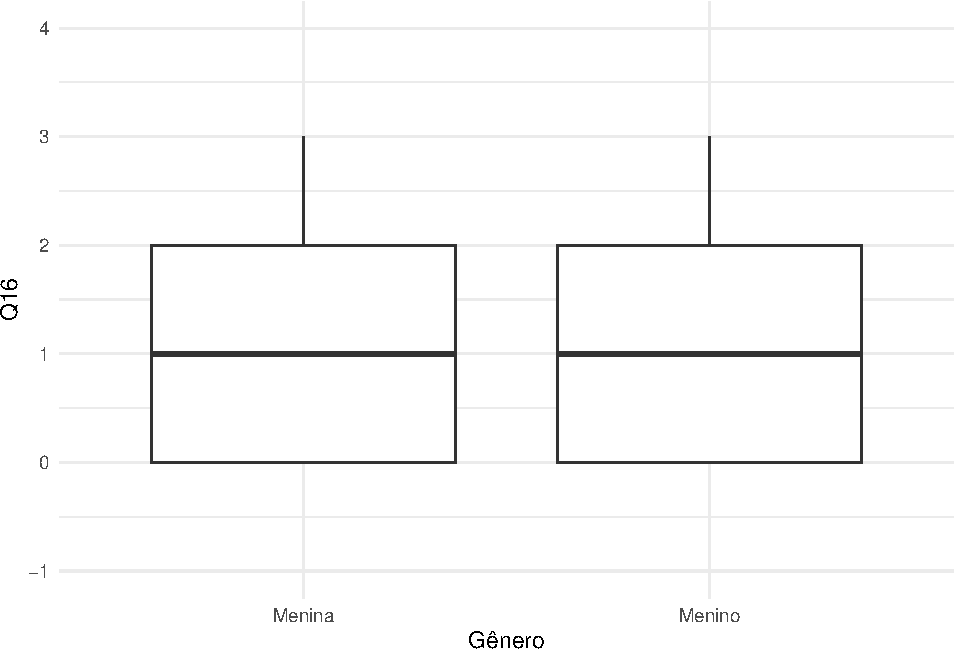
\includegraphics[width=0.75\linewidth]{relatorio_covid19_files/figure-latex/unnamed-chunk-146-1} \end{center}

\hypertarget{teste-de-kruskal-wallis-de-q16-por-guxeanero}{%
\paragraph{Teste de Kruskal-Wallis de Q16 por Gênero}\label{teste-de-kruskal-wallis-de-q16-por-guxeanero}}

Apenas seis crianças se identificaram com o gênero \emph{outros} e foram removidas na análise estatística.

Como o valor-p é maior ou igual a 0.01 (nível de significância), não rejeitamos a hipótese nula e as medianas de Q16 entre meninos e meninas são iguais.

\begin{longtable}[]{@{}ccc@{}}
\caption{\label{tab:unnamed-chunk-148}Valores-p para comparação múltipla de medianas: Q16 e Gênero.}\tabularnewline
\toprule
Estatística & Parâmetro & valor p\tabularnewline
\midrule
\endfirsthead
\toprule
Estatística & Parâmetro & valor p\tabularnewline
\midrule
\endhead
0,09 & 1 & 0,76\tabularnewline
\bottomrule
\end{longtable}

\hypertarget{teste-de-nemeyi-de-q16-por-guxeanero}{%
\paragraph{Teste de Nemeyi de Q16 por Gênero}\label{teste-de-nemeyi-de-q16-por-guxeanero}}

Apenas seis crianças se identificaram com o gênero \emph{outros} e foram removidas na análise estatística.

Como os valores-p são iguais ou maiores que 0.01 (nível de significância), não rejeitamos a hipótese nula e as medianas de Q16 entre meninos e meninas são iguais.

\begin{longtable}[]{@{}lc@{}}
\caption{\label{tab:unnamed-chunk-150}valores-p para o teste de comparação múltipla de Nemeyi de Q16 por Gênero.}\tabularnewline
\toprule
& Menina\tabularnewline
\midrule
\endfirsthead
\toprule
& Menina\tabularnewline
\midrule
\endhead
Menino & 0,77\tabularnewline
\bottomrule
\end{longtable}

\cleardoublepage

\hypertarget{tabela-de-continguxeancia-idade-e-q16}{%
\paragraph{Tabela de contingência: Idade e Q16}\label{tabela-de-continguxeancia-idade-e-q16}}

\begin{longtable}[]{@{}ccccc@{}}
\caption{\label{tab:unnamed-chunk-151}Tabela de contingência: Idade e Q16.}\tabularnewline
\toprule
Idade & Muita preocupação & Pouca preocupação & Sem preocupação & Sem resposta\tabularnewline
\midrule
\endfirsthead
\toprule
Idade & Muita preocupação & Pouca preocupação & Sem preocupação & Sem resposta\tabularnewline
\midrule
\endhead
8 & 64 & 63 & 65 & 3\tabularnewline
9 & 66 & 54 & 65 & 1\tabularnewline
10 & 86 & 84 & 73 & 7\tabularnewline
11 & 68 & 92 & 78 & 2\tabularnewline
12 & 44 & 59 & 73 & 3\tabularnewline
\bottomrule
\end{longtable}

\hypertarget{gruxe1fico-de-barras-idade-e-q16}{%
\paragraph{Gráfico de barras: Idade e Q16}\label{gruxe1fico-de-barras-idade-e-q16}}

\begin{center}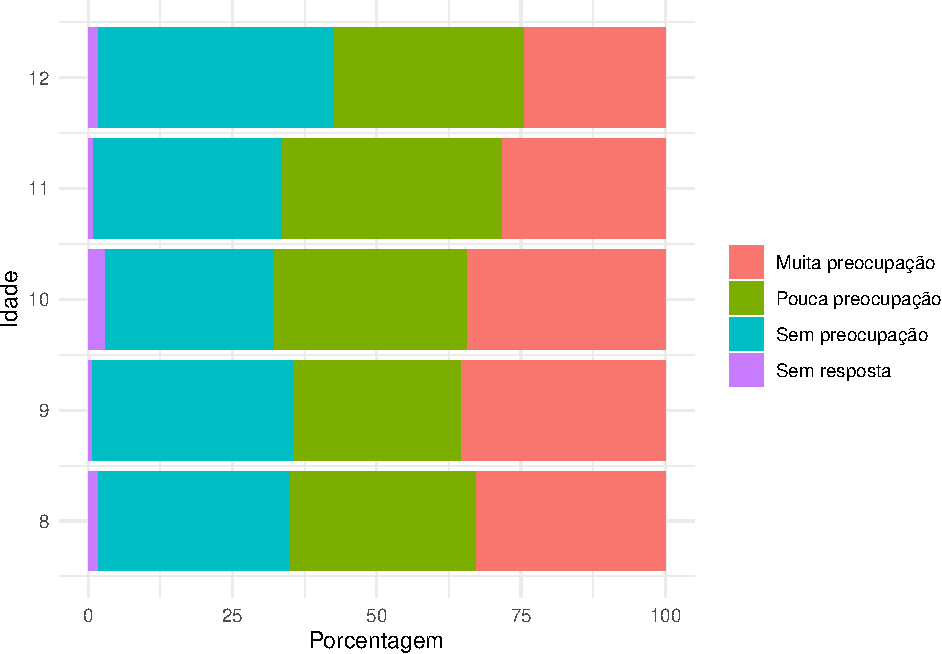
\includegraphics[width=0.75\linewidth]{relatorio_covid19_files/figure-latex/unnamed-chunk-152-1} \end{center}

\hypertarget{teste-qui-quadrado-14}{%
\paragraph{Teste qui-quadrado}\label{teste-qui-quadrado-14}}

Como o valor-p é igual ou maior que 0.01 (nível de significância), não rejeitamos a hipótese nula e não temos evidência estatística que as duas variáveis estão associadas.

\begin{longtable}[]{@{}ccc@{}}
\caption{\label{tab:unnamed-chunk-154}Teste qui-quadrado entre Idade e Q16.}\tabularnewline
\toprule
Estatística & Graus de liberdade & Valor-p\tabularnewline
\midrule
\endfirsthead
\toprule
Estatística & Graus de liberdade & Valor-p\tabularnewline
\midrule
\endhead
17,09 & 12 & 0,15\tabularnewline
\bottomrule
\end{longtable}

\cleardoublepage

\hypertarget{medidas-de-resumo-q16-por-idade}{%
\paragraph{Medidas de Resumo Q16 por Idade}\label{medidas-de-resumo-q16-por-idade}}

\begin{longtable}[]{@{}cccccc@{}}
\caption{\label{tab:unnamed-chunk-155}Medidas de resumo de Q16 por Idade.}\tabularnewline
\toprule
Q16 & Média & Desvio Padrão & Mediana & 1 Quartil & 3 Quartil\tabularnewline
\midrule
\endfirsthead
\toprule
Q16 & Média & Desvio Padrão & Mediana & 1 Quartil & 3 Quartil\tabularnewline
\midrule
\endhead
8 & 1,03 & 0,85 & 1 & 0 & 2\tabularnewline
9 & 1,02 & 0,85 & 1 & 0 & 2\tabularnewline
10 & 1,11 & 0,86 & 1 & 0 & 2\tabularnewline
11 & 0,98 & 0,80 & 1 & 0 & 2\tabularnewline
12 & 0,87 & 0,84 & 1 & 0 & 2\tabularnewline
\bottomrule
\end{longtable}

\hypertarget{boxplot-de-q16-por-idade}{%
\paragraph{Boxplot de Q16 por Idade}\label{boxplot-de-q16-por-idade}}

\begin{center}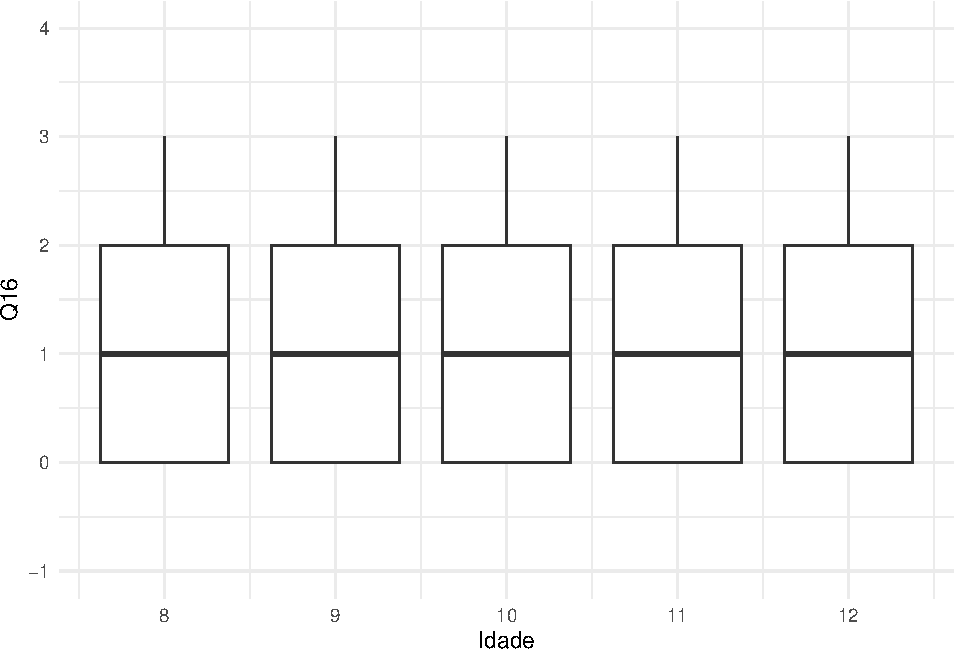
\includegraphics[width=0.75\linewidth]{relatorio_covid19_files/figure-latex/unnamed-chunk-156-1} \end{center}

\hypertarget{teste-de-kruskal-wallis-de-q16-por-idade}{%
\paragraph{Teste de Kruskal-Wallis de Q16 por Idade}\label{teste-de-kruskal-wallis-de-q16-por-idade}}

Como o valor-p é maior ou igual a 0.01 (nível de significância), não rejeitamos a hipótese nula e as medianas de Q16 entre as idades são iguais.

\begin{longtable}[]{@{}ccc@{}}
\caption{\label{tab:unnamed-chunk-158}Valores-p para comparação múltipla de medianas: Q16 e Idade.}\tabularnewline
\toprule
Estatística & Parâmetro & valor p\tabularnewline
\midrule
\endfirsthead
\toprule
Estatística & Parâmetro & valor p\tabularnewline
\midrule
\endhead
8,54 & 4 & 0,07\tabularnewline
\bottomrule
\end{longtable}

\hypertarget{teste-de-nemeyi-de-q16-por-idade}{%
\paragraph{Teste de Nemeyi de Q16 por Idade}\label{teste-de-nemeyi-de-q16-por-idade}}

Como os valores-p são iguais ou maiores que 0.01 (nível de significância), não rejeitamos a hipótese nula e as medianas de Q16 entre pares de crianças de diferentes idades são todas iguais.

\begin{longtable}[]{@{}lcccc@{}}
\caption{\label{tab:unnamed-chunk-160}Teste de Nemeyi de Q16 por Idade.}\tabularnewline
\toprule
& 8 & 9 & 10 & 11\tabularnewline
\midrule
\endfirsthead
\toprule
& 8 & 9 & 10 & 11\tabularnewline
\midrule
\endhead
9 & 1,00 & & &\tabularnewline
10 & 0,89 & 0,87 & &\tabularnewline
11 & 0,98 & 0,99 & 0,53 &\tabularnewline
12 & 0,43 & 0,48 & 0,05 & 0,72\tabularnewline
\bottomrule
\end{longtable}

\cleardoublepage

\hypertarget{tabela-de-continguxeancia-rauxe7a-e-q16}{%
\paragraph{Tabela de contingência: Raça e Q16}\label{tabela-de-continguxeancia-rauxe7a-e-q16}}

\begin{longtable}[]{@{}ccccc@{}}
\caption{\label{tab:unnamed-chunk-161}Tabela de contingência: Raça e Q16.}\tabularnewline
\toprule
Raça & Muita preocupação & Pouca preocupação & Sem preocupação & Sem resposta\tabularnewline
\midrule
\endfirsthead
\toprule
Raça & Muita preocupação & Pouca preocupação & Sem preocupação & Sem resposta\tabularnewline
\midrule
\endhead
Amarela & 5 & 8 & 4 & 2\tabularnewline
Branca & 49 & 55 & 109 &\tabularnewline
Indígena & 7 & 8 & 6 &\tabularnewline
Negra & 256 & 269 & 210 & 14\tabularnewline
Outros & 4 & 4 & 8 &\tabularnewline
Sem resposta & 7 & 8 & 17 &\tabularnewline
\bottomrule
\end{longtable}

\hypertarget{gruxe1fico-de-barras-rauxe7a-e-q16}{%
\paragraph{Gráfico de barras: Raça e Q16}\label{gruxe1fico-de-barras-rauxe7a-e-q16}}

\begin{center}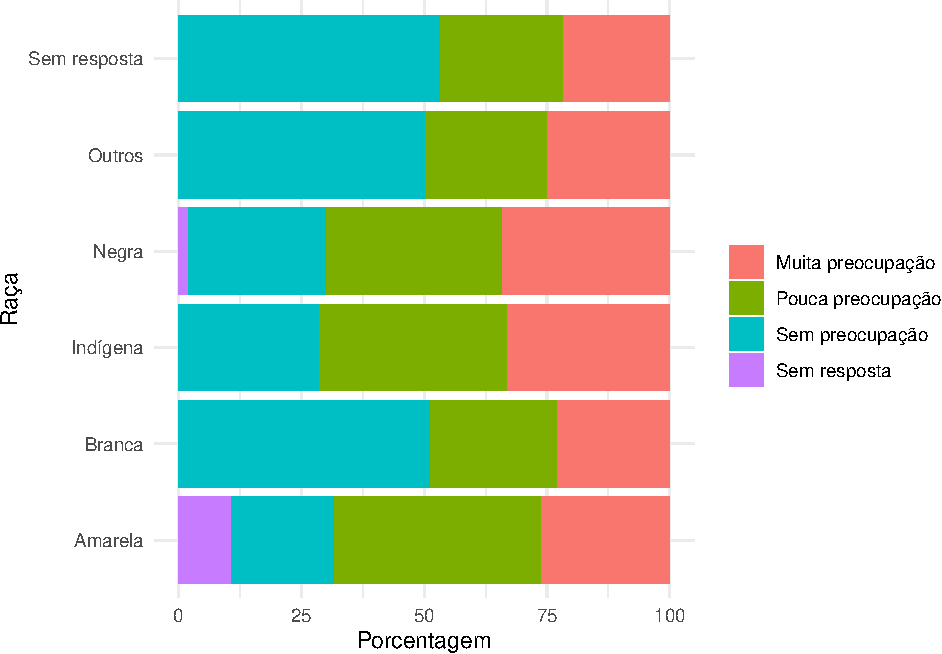
\includegraphics[width=0.75\linewidth]{relatorio_covid19_files/figure-latex/unnamed-chunk-162-1} \end{center}

\hypertarget{teste-qui-quadrado-15}{%
\paragraph{Teste qui-quadrado}\label{teste-qui-quadrado-15}}

Como o valor-p é menor que 0.01 (nível de significância), rejeitamos a hipótese nula e temos evidência estatística que as duas variáveis estão associadas.

\begin{longtable}[]{@{}ccc@{}}
\caption{\label{tab:unnamed-chunk-164}Teste qui-quadrado entre raca e Q16.}\tabularnewline
\toprule
Estatística & Graus de liberdade & Valor-p\tabularnewline
\midrule
\endfirsthead
\toprule
Estatística & Graus de liberdade & Valor-p\tabularnewline
\midrule
\endhead
61,92 & 15 & 0\tabularnewline
\bottomrule
\end{longtable}

\cleardoublepage

\hypertarget{medidas-de-resumo-q16-por-rauxe7a}{%
\paragraph{Medidas de Resumo Q16 por Raça}\label{medidas-de-resumo-q16-por-rauxe7a}}

\begin{longtable}[]{@{}cccccc@{}}
\caption{\label{tab:unnamed-chunk-165}Medidas de resumo de Q16 por raca.}\tabularnewline
\toprule
Q16 & Média & Desvio Padrão & Mediana & 1 Quartil & 3 Quartil\tabularnewline
\midrule
\endfirsthead
\toprule
Q16 & Média & Desvio Padrão & Mediana & 1 Quartil & 3 Quartil\tabularnewline
\midrule
\endhead
Amarela & 1,26 & 0,93 & 1,0 & 1 & 2,00\tabularnewline
Branca & 0,72 & 0,82 & 0,0 & 0 & 1,00\tabularnewline
Indígena & 1,05 & 0,80 & 1,0 & 0 & 2,00\tabularnewline
Negra & 1,10 & 0,83 & 1,0 & 0 & 2,00\tabularnewline
Outros & 0,75 & 0,86 & 0,5 & 0 & 1,25\tabularnewline
Sem resposta & 0,69 & 0,82 & 0,0 & 0 & 1,00\tabularnewline
\bottomrule
\end{longtable}

\hypertarget{boxplot-de-q16-por-rauxe7a}{%
\paragraph{Boxplot de Q16 por Raça}\label{boxplot-de-q16-por-rauxe7a}}

\begin{center}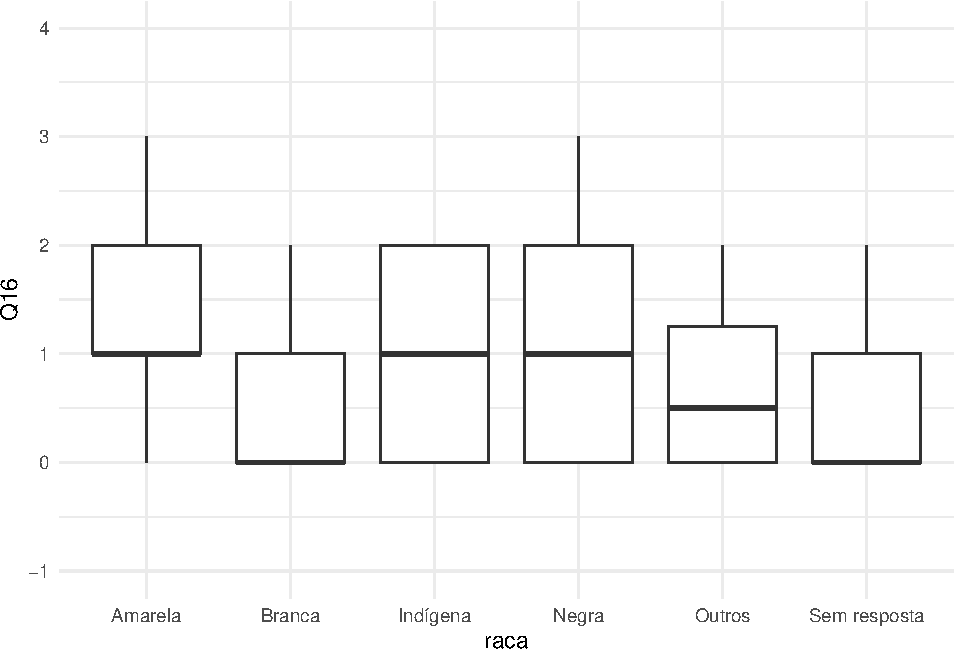
\includegraphics[width=0.75\linewidth]{relatorio_covid19_files/figure-latex/unnamed-chunk-166-1} \end{center}

\hypertarget{teste-de-kruskal-wallis-de-q16-por-rauxe7a}{%
\paragraph{Teste de Kruskal-Wallis de Q16 por Raça}\label{teste-de-kruskal-wallis-de-q16-por-rauxe7a}}

Como o valor-p é menor que 0.01 (nível de significância), rejeitamos a hipótese nula e as medianas de Q16 entre raças não são todas iguais.

\begin{longtable}[]{@{}ccc@{}}
\caption{\label{tab:unnamed-chunk-168}Valores-p para comparação múltipla de medianas: Q16 e Raça.}\tabularnewline
\toprule
Estatística & Parâmetro & valor p\tabularnewline
\midrule
\endfirsthead
\toprule
Estatística & Parâmetro & valor p\tabularnewline
\midrule
\endhead
41,19 & 5 & 0\tabularnewline
\bottomrule
\end{longtable}

\hypertarget{teste-de-nemeyi-de-q16-por-rauxe7a}{%
\paragraph{Teste de Nemeyi de Q16 por Raça}\label{teste-de-nemeyi-de-q16-por-rauxe7a}}

Existem valores-p menores que 0.01 (nível de significância), e para estes pares rejeitamos a hipótese nula e as medianas de Q16 entre estes pares de raças são diferentes.

\begin{longtable}[]{@{}lccccc@{}}
\caption{\label{tab:unnamed-chunk-170}Valores-p para o teste de Nemeyi de Q16 por Raça.}\tabularnewline
\toprule
& Amarela & Branca & Indígena & Negra & Outros\tabularnewline
\midrule
\endfirsthead
\toprule
& Amarela & Branca & Indígena & Negra & Outros\tabularnewline
\midrule
\endhead
Branca & 0,17 & & & &\tabularnewline
Indígena & 0,99 & 0,56 & & &\tabularnewline
Negra & 0,99 & 0,00 & 1,00 & &\tabularnewline
Outros & 0,62 & 1,00 & 0,91 & 0,64 &\tabularnewline
Sem resposta & 0,30 & 1,00 & 0,68 & 0,11 & 1\tabularnewline
\bottomrule
\end{longtable}

\cleardoublepage

\hypertarget{tabela-de-continguxeancia-tipo-de-escola-e-q16}{%
\paragraph{Tabela de contingência: Tipo de escola e Q16}\label{tabela-de-continguxeancia-tipo-de-escola-e-q16}}

Apenas sete crianças não estavam matriculadas na escola, e foram retiradas da análise para facilitar a análise de \emph{tipo de escola}.

\begin{longtable}[]{@{}ccccc@{}}
\caption{\label{tab:unnamed-chunk-171}Tabela de contingência: Tipo de escola e Q16.}\tabularnewline
\toprule
\begin{minipage}[b]{0.16\columnwidth}\centering
Tipo de Escola\strut
\end{minipage} & \begin{minipage}[b]{0.19\columnwidth}\centering
Muita preocupação\strut
\end{minipage} & \begin{minipage}[b]{0.19\columnwidth}\centering
Pouca preocupação\strut
\end{minipage} & \begin{minipage}[b]{0.17\columnwidth}\centering
Sem preocupação\strut
\end{minipage} & \begin{minipage}[b]{0.14\columnwidth}\centering
Sem resposta\strut
\end{minipage}\tabularnewline
\midrule
\endfirsthead
\toprule
\begin{minipage}[b]{0.16\columnwidth}\centering
Tipo de Escola\strut
\end{minipage} & \begin{minipage}[b]{0.19\columnwidth}\centering
Muita preocupação\strut
\end{minipage} & \begin{minipage}[b]{0.19\columnwidth}\centering
Pouca preocupação\strut
\end{minipage} & \begin{minipage}[b]{0.17\columnwidth}\centering
Sem preocupação\strut
\end{minipage} & \begin{minipage}[b]{0.14\columnwidth}\centering
Sem resposta\strut
\end{minipage}\tabularnewline
\midrule
\endhead
\begin{minipage}[t]{0.16\columnwidth}\centering
Particular\strut
\end{minipage} & \begin{minipage}[t]{0.19\columnwidth}\centering
134\strut
\end{minipage} & \begin{minipage}[t]{0.19\columnwidth}\centering
169\strut
\end{minipage} & \begin{minipage}[t]{0.17\columnwidth}\centering
278\strut
\end{minipage} & \begin{minipage}[t]{0.14\columnwidth}\centering
9\strut
\end{minipage}\tabularnewline
\begin{minipage}[t]{0.16\columnwidth}\centering
Pública\strut
\end{minipage} & \begin{minipage}[t]{0.19\columnwidth}\centering
194\strut
\end{minipage} & \begin{minipage}[t]{0.19\columnwidth}\centering
179\strut
\end{minipage} & \begin{minipage}[t]{0.17\columnwidth}\centering
73\strut
\end{minipage} & \begin{minipage}[t]{0.14\columnwidth}\centering
7\strut
\end{minipage}\tabularnewline
\bottomrule
\end{longtable}

\hypertarget{gruxe1fico-de-barras-tipo-de-escola-e-q16}{%
\paragraph{Gráfico de barras: Tipo de escola e Q16}\label{gruxe1fico-de-barras-tipo-de-escola-e-q16}}

Apenas sete crianças não estavam matriculadas na escola, e foram retiradas da análise para facilitar a análise de \emph{tipo de escola}.

\begin{center}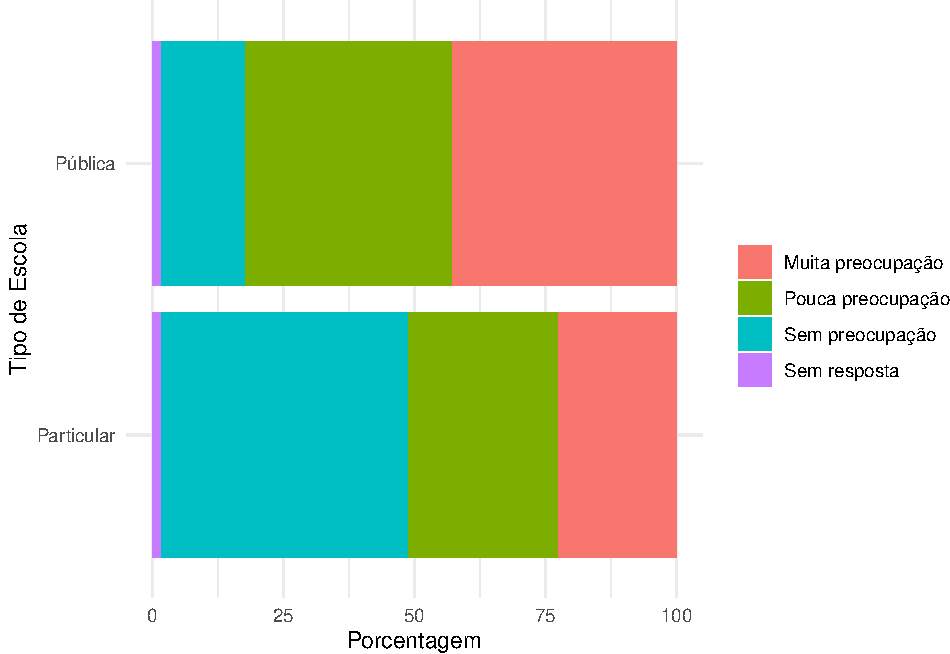
\includegraphics[width=0.75\linewidth]{relatorio_covid19_files/figure-latex/unnamed-chunk-172-1} \end{center}

\hypertarget{teste-qui-quadrado-16}{%
\paragraph{Teste qui-quadrado}\label{teste-qui-quadrado-16}}

Apenas sete crianças não estavam matriculadas na escola, e foram retiradas da análise para facilitar a análise de \emph{tipo de escola}.

Como o valor-p é menor que 0.01 (nível de significância), rejeitamos a hipótese nula e temos evidência estatística que as duas variáveis estão associadas.

\begin{longtable}[]{@{}ccc@{}}
\caption{\label{tab:unnamed-chunk-174}Teste qui-quadrado entre Escola e Q16.}\tabularnewline
\toprule
Estatística & Graus de liberdade & Valor-p\tabularnewline
\midrule
\endfirsthead
\toprule
Estatística & Graus de liberdade & Valor-p\tabularnewline
\midrule
\endhead
115,24 & 3 & 0\tabularnewline
\bottomrule
\end{longtable}

\cleardoublepage

\hypertarget{medidas-de-resumo-q16-por-tipo-de-escola}{%
\paragraph{Medidas de Resumo Q16 por Tipo de escola}\label{medidas-de-resumo-q16-por-tipo-de-escola}}

Apenas sete crianças não estavam matriculadas na escola, e foram retiradas da análise para facilitar a análise de \emph{tipo de escola}.

\begin{longtable}[]{@{}cccccc@{}}
\caption{\label{tab:unnamed-chunk-175}Medidas de resumo de Q16 por Escola.}\tabularnewline
\toprule
Q16 & Média & Desvio Padrão & Mediana & 1 Quartil & 3 Quartil\tabularnewline
\midrule
\endfirsthead
\toprule
Q16 & Média & Desvio Padrão & Mediana & 1 Quartil & 3 Quartil\tabularnewline
\midrule
\endhead
Particular & 0,79 & 0,85 & 1 & 0 & 1\tabularnewline
Pública & 1,30 & 0,75 & 1 & 1 & 2\tabularnewline
\bottomrule
\end{longtable}

\hypertarget{boxplot-de-q16-por-tipo-de-escola}{%
\paragraph{Boxplot de Q16 por Tipo de escola}\label{boxplot-de-q16-por-tipo-de-escola}}

Apenas sete crianças não estavam matriculadas na escola, e foram retiradas da análise para facilitar a análise de \emph{tipo de escola}.

\begin{center}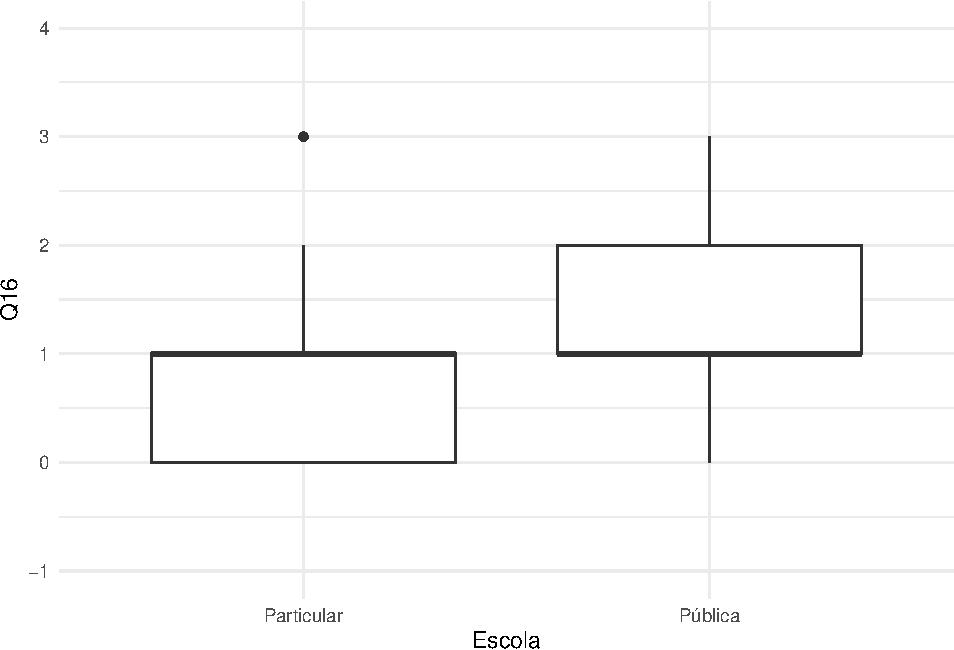
\includegraphics[width=0.75\linewidth]{relatorio_covid19_files/figure-latex/unnamed-chunk-176-1} \end{center}

\hypertarget{teste-de-kruskal-wallis-de-q16-por-tipo-de-escola}{%
\paragraph{Teste de Kruskal-Wallis de Q16 por Tipo de escola}\label{teste-de-kruskal-wallis-de-q16-por-tipo-de-escola}}

Apenas sete crianças não estavam matriculadas na escola, e foram retiradas da análise para facilitar a análise de \emph{tipo de escola}.

Como o valor-p é menor que 0.01 (nível de significância), rejeitamos a hipótese nula e as medianas de Q16 entre tipos de escola são diferentes.

\begin{longtable}[]{@{}ccc@{}}
\caption{\label{tab:unnamed-chunk-178}Valores-p para comparação múltipla de medianas: Q16 e Tipo de escola.}\tabularnewline
\toprule
Estatística & Parâmetro & valor p\tabularnewline
\midrule
\endfirsthead
\toprule
Estatística & Parâmetro & valor p\tabularnewline
\midrule
\endhead
98,38 & 1 & 0\tabularnewline
\bottomrule
\end{longtable}

\hypertarget{teste-de-nemeyi-de-q16-por-tipo-de-escola}{%
\paragraph{Teste de Nemeyi de Q16 por Tipo de escola}\label{teste-de-nemeyi-de-q16-por-tipo-de-escola}}

Apenas sete crianças não estavam matriculadas na escola, e foram retiradas da análise para facilitar a análise de \emph{tipo de escola}.

O valor-p é maior ou igual que 0.01 (nível de significância), e rejeitamos a hipótese nula e as medianas de Q16 entre tipos de escolas são diferentes.

\begin{longtable}[]{@{}lc@{}}
\caption{\label{tab:unnamed-chunk-180}Teste de Nemeyi de Q16 por Escola.}\tabularnewline
\toprule
& Particular\tabularnewline
\midrule
\endfirsthead
\toprule
& Particular\tabularnewline
\midrule
\endhead
Pública & 0\tabularnewline
\bottomrule
\end{longtable}

\cleardoublepage

\hypertarget{q17}{%
\subsection{Q17}\label{q17}}

A variável Q17 corresponde ao campo de númeo 13 com enunciado \textbf{O quanto você está preocupado hoje com as questões abaixo} no quesito:

\begin{itemize}
\tightlist
\item
  \emph{Que pessoas da minha família fiquem doentes com o coronavírus}
\end{itemize}

\hypertarget{anuxe1lise-descritiva-para-q17}{%
\subsubsection{Análise descritiva para Q17}\label{anuxe1lise-descritiva-para-q17}}

\hypertarget{gruxe1fico-de-barras-q17}{%
\paragraph{Gráfico de barras: Q17}\label{gruxe1fico-de-barras-q17}}

\begin{center}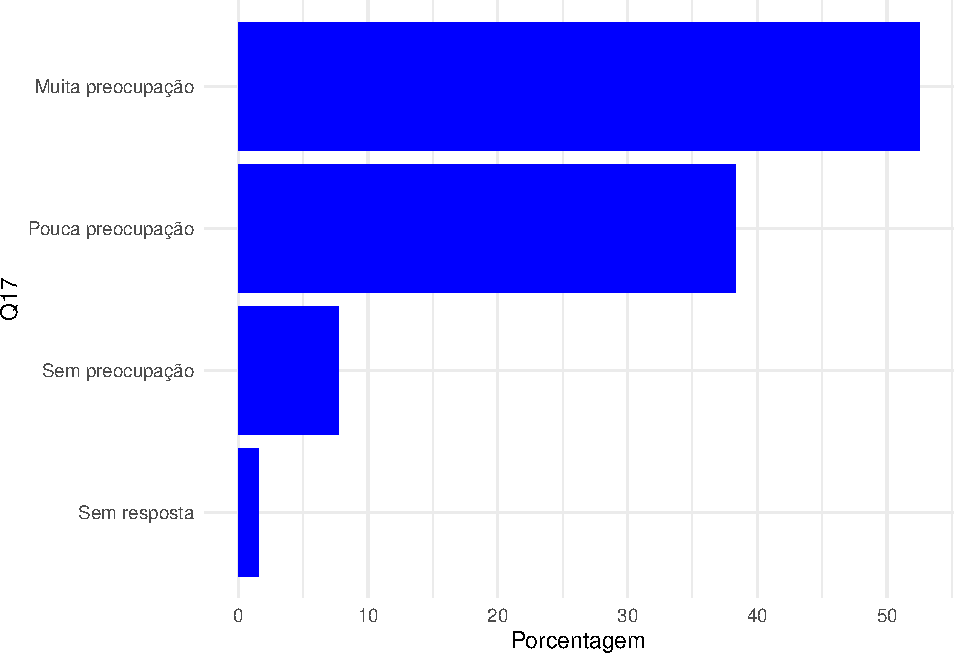
\includegraphics[width=0.75\linewidth]{relatorio_covid19_files/figure-latex/unnamed-chunk-187-1} \end{center}

\hypertarget{tabela-de-distribuiuxe7uxe3o-q17}{%
\paragraph{Tabela de distribuição: Q17}\label{tabela-de-distribuiuxe7uxe3o-q17}}

\begin{longtable}[]{@{}cccc@{}}
\caption{\label{tab:unnamed-chunk-188}Que pessoas da minha família fiquem doentes com o coronavírus}\tabularnewline
\toprule
Q17 & Frequência & Frequência relativa & Porcentagem\tabularnewline
\midrule
\endfirsthead
\toprule
Q17 & Frequência & Frequência relativa & Porcentagem\tabularnewline
\midrule
\endhead
Muita preocupação & 551 & 0,52 & 52,48\tabularnewline
Pouca preocupação & 402 & 0,38 & 38,29\tabularnewline
Sem preocupação & 81 & 0,08 & 7,71\tabularnewline
Sem resposta & 16 & 0,02 & 1,52\tabularnewline
\bottomrule
\end{longtable}

\hypertarget{medidas-de-resumo-q17}{%
\paragraph{Medidas de resumo: Q17}\label{medidas-de-resumo-q17}}

\begin{longtable}[]{@{}ccccc@{}}
\caption{\label{tab:unnamed-chunk-189}Resumos para variável Q17.}\tabularnewline
\toprule
Média & Desvio Padrão & Mediana & 1Qua & 3Qua\tabularnewline
\midrule
\endfirsthead
\toprule
Média & Desvio Padrão & Mediana & 1Qua & 3Qua\tabularnewline
\midrule
\endhead
1,48 & 0,66 & 2 & 1 & 2\tabularnewline
\bottomrule
\end{longtable}

\cleardoublepage

\hypertarget{anuxe1lise-bidimensional-q17}{%
\subsubsection{Análise bidimensional Q17}\label{anuxe1lise-bidimensional-q17}}

\hypertarget{tabela-de-continguxeancia-cidade-e-q17}{%
\paragraph{Tabela de contingência: Cidade e Q17}\label{tabela-de-continguxeancia-cidade-e-q17}}

\begin{longtable}[]{@{}ccccc@{}}
\caption{\label{tab:unnamed-chunk-190}Tabela de contingência: Cidade e Q17.}\tabularnewline
\toprule
Cidade & Muita preocupação & Pouca preocupação & Sem preocupação & Sem resposta\tabularnewline
\midrule
\endfirsthead
\toprule
Cidade & Muita preocupação & Pouca preocupação & Sem preocupação & Sem resposta\tabularnewline
\midrule
\endhead
Camaçari & 72 & 77 & 40 & 8\tabularnewline
Candeias & 12 & 15 & 9 & 2\tabularnewline
Lauro de Freitas & 11 & 26 & 23 & 1\tabularnewline
Outros & 23 & 41 & 19 &\tabularnewline
Pojuca & 25 & 27 & 10 & 2\tabularnewline
Salvador & 113 & 225 & 217 & 18\tabularnewline
Simões Filho & 9 & 17 & 7 & 1\tabularnewline
\bottomrule
\end{longtable}

\hypertarget{gruxe1fico-de-barras-cidade-e-q17}{%
\paragraph{Gráfico de barras: Cidade e Q17}\label{gruxe1fico-de-barras-cidade-e-q17}}

\begin{center}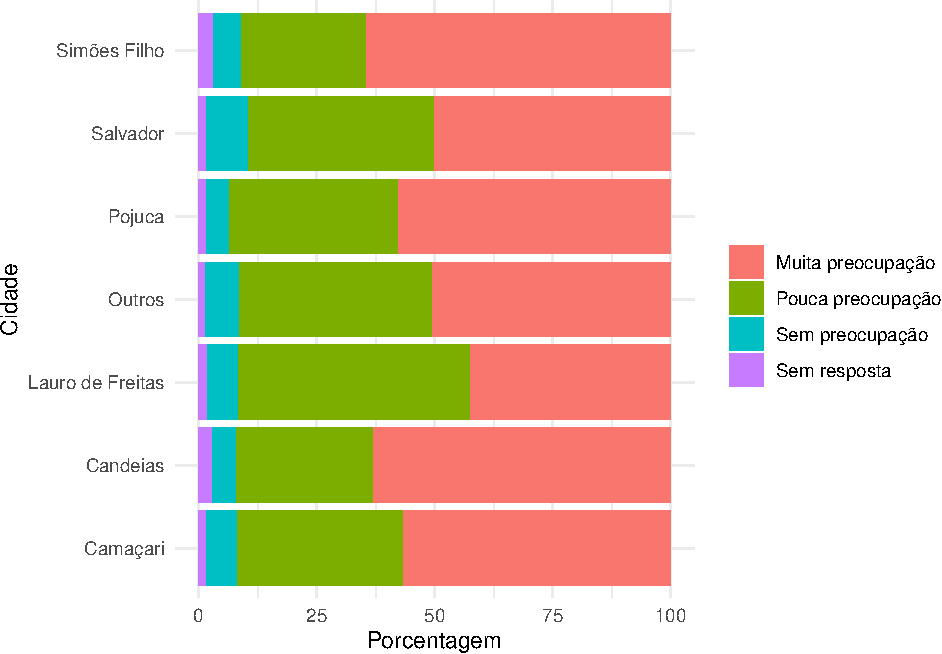
\includegraphics[width=0.75\linewidth]{relatorio_covid19_files/figure-latex/unnamed-chunk-191-1} \end{center}

\hypertarget{teste-qui-quadrado-17}{%
\paragraph{Teste qui-quadrado}\label{teste-qui-quadrado-17}}

Como o valor-p é igual igual ou maior que 0.01 (nível de significância), não rejeitamos a hipótese nula e não temos evidência estatística que as duas variáveis estão associadas.

\begin{longtable}[]{@{}ccc@{}}
\caption{\label{tab:unnamed-chunk-193}Teste qui-quadrado entre Cidade e Q17.}\tabularnewline
\toprule
Estatística & Graus de liberdade & Valor-p\tabularnewline
\midrule
\endfirsthead
\toprule
Estatística & Graus de liberdade & Valor-p\tabularnewline
\midrule
\endhead
13,15 & 18 & 0,78\tabularnewline
\bottomrule
\end{longtable}

\cleardoublepage

\hypertarget{medidas-de-resumo-q17-por-cidade}{%
\paragraph{Medidas de Resumo Q17 por Cidade}\label{medidas-de-resumo-q17-por-cidade}}

\begin{longtable}[]{@{}cccccc@{}}
\caption{\label{tab:unnamed-chunk-194}Medidas de resumo de Q17 por Cidade.}\tabularnewline
\toprule
Q17 & Média & Desvio Padrão & Mediana & 1 Quartil & 3 Quartil\tabularnewline
\midrule
\endfirsthead
\toprule
Q17 & Média & Desvio Padrão & Mediana & 1 Quartil & 3 Quartil\tabularnewline
\midrule
\endhead
Camaçari & 1,53 & 0,64 & 2 & 1 & 2\tabularnewline
Candeias & 1,63 & 0,63 & 2 & 1 & 2\tabularnewline
Lauro de Freitas & 1,39 & 0,64 & 1 & 1 & 2\tabularnewline
Outros & 1,46 & 0,65 & 2 & 1 & 2\tabularnewline
Pojuca & 1,56 & 0,61 & 2 & 1 & 2\tabularnewline
Salvador & 1,44 & 0,67 & 2 & 1 & 2\tabularnewline
Simões Filho & 1,65 & 0,65 & 2 & 1 & 2\tabularnewline
\bottomrule
\end{longtable}

\hypertarget{boxplot-de-q17-por-cidade}{%
\paragraph{Boxplot de Q17 por Cidade}\label{boxplot-de-q17-por-cidade}}

\begin{center}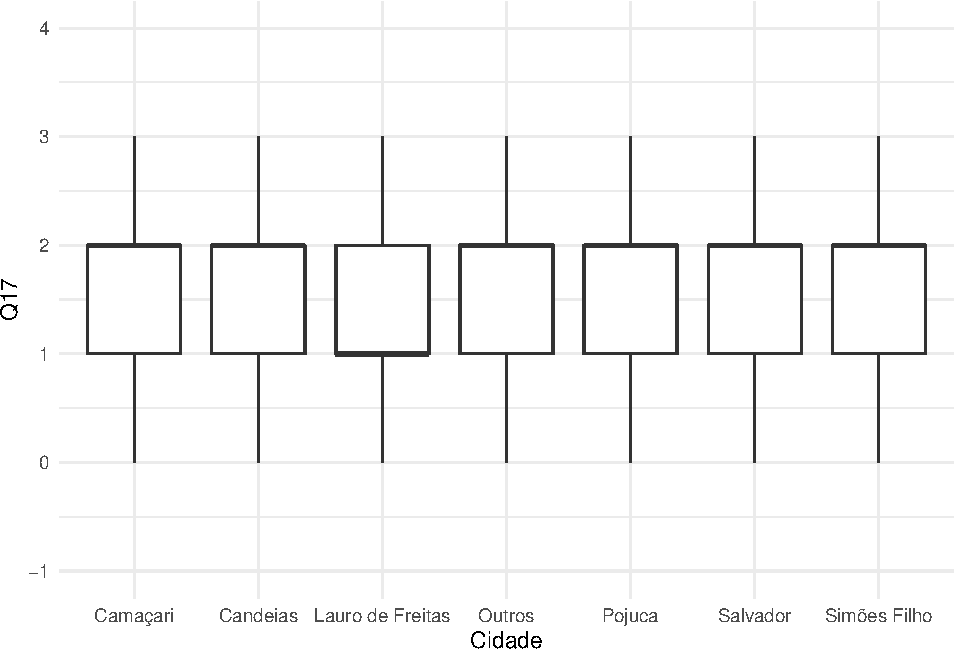
\includegraphics[width=0.75\linewidth]{relatorio_covid19_files/figure-latex/unnamed-chunk-195-1} \end{center}

\hypertarget{teste-de-kruskal-wallis-de-q17-por-cidade}{%
\paragraph{Teste de Kruskal-Wallis de Q17 por Cidade}\label{teste-de-kruskal-wallis-de-q17-por-cidade}}

Como o valor-p é maior ou igual a 0.01 (nível de significância), não rejeitamos a hipótese nula e as medianas de Q17 entre as crianças de diversas cidades são todas iguais.

\begin{longtable}[]{@{}ccc@{}}
\caption{\label{tab:unnamed-chunk-197}Valor-p para o teste de Kruskal-Wallis: Q17 e Cidade.}\tabularnewline
\toprule
Estatística & Parâmetro & valor p\tabularnewline
\midrule
\endfirsthead
\toprule
Estatística & Parâmetro & valor p\tabularnewline
\midrule
\endhead
10,42 & 6 & 0,11\tabularnewline
\bottomrule
\end{longtable}

\hypertarget{teste-de-nemeyi-de-q17-por-cidade}{%
\paragraph{Teste de Nemeyi de Q17 por Cidade}\label{teste-de-nemeyi-de-q17-por-cidade}}

Como os valores-p são iguais ou maiores que 0.01 (nível de significância), não rejeitamos a hipótese nula e as medianas de Q17 entre as crianças de diversas cidades são iguais.

\begin{longtable}[]{@{}lcccccc@{}}
\caption{\label{tab:unnamed-chunk-199}Valores-p para o teste de comparação múltipla de Nemeyi de Q17 por Cidade.}\tabularnewline
\toprule
& Camaçari & Candeias & Lauro de Freitas & Outros & Pojuca & Salvador\tabularnewline
\midrule
\endfirsthead
\toprule
& Camaçari & Candeias & Lauro de Freitas & Outros & Pojuca & Salvador\tabularnewline
\midrule
\endhead
Candeias & 0,99 & & & & &\tabularnewline
Lauro de Freitas & 0,74 & 0,59 & & & &\tabularnewline
Outros & 0,98 & 0,87 & 1,00 & & &\tabularnewline
Pojuca & 1,00 & 1,00 & 0,80 & 0,98 & &\tabularnewline
Salvador & 0,74 & 0,70 & 0,99 & 1,00 & 0,9 &\tabularnewline
Simões Filho & 0,97 & 1,00 & 0,55 & 0,83 & 1,0 & 0,66\tabularnewline
\bottomrule
\end{longtable}

\cleardoublepage

\hypertarget{tabela-de-continguxeancia-guxeanero-e-q17}{%
\paragraph{Tabela de contingência: Gênero e Q17}\label{tabela-de-continguxeancia-guxeanero-e-q17}}

Apenas seis crianças se identificaram com o gênero \emph{outros} e foram removidas na análise estatística.

\begin{longtable}[]{@{}ccccc@{}}
\caption{\label{tab:unnamed-chunk-200}Tabela de contingência: Gênero e Q17.}\tabularnewline
\toprule
Gênero & Muita preocupação & Pouca preocupação & Sem preocupação & Sem resposta\tabularnewline
\midrule
\endfirsthead
\toprule
Gênero & Muita preocupação & Pouca preocupação & Sem preocupação & Sem resposta\tabularnewline
\midrule
\endhead
Menina & 299 & 199 & 36 & 7\tabularnewline
Menino & 249 & 201 & 44 & 9\tabularnewline
\bottomrule
\end{longtable}

\hypertarget{gruxe1fico-de-barras-guxeanero-e-q17}{%
\paragraph{Gráfico de barras: Gênero e Q17}\label{gruxe1fico-de-barras-guxeanero-e-q17}}

Apenas seis crianças se identificaram com o gênero \emph{outros} e foram removidas na análise estatística.

\begin{center}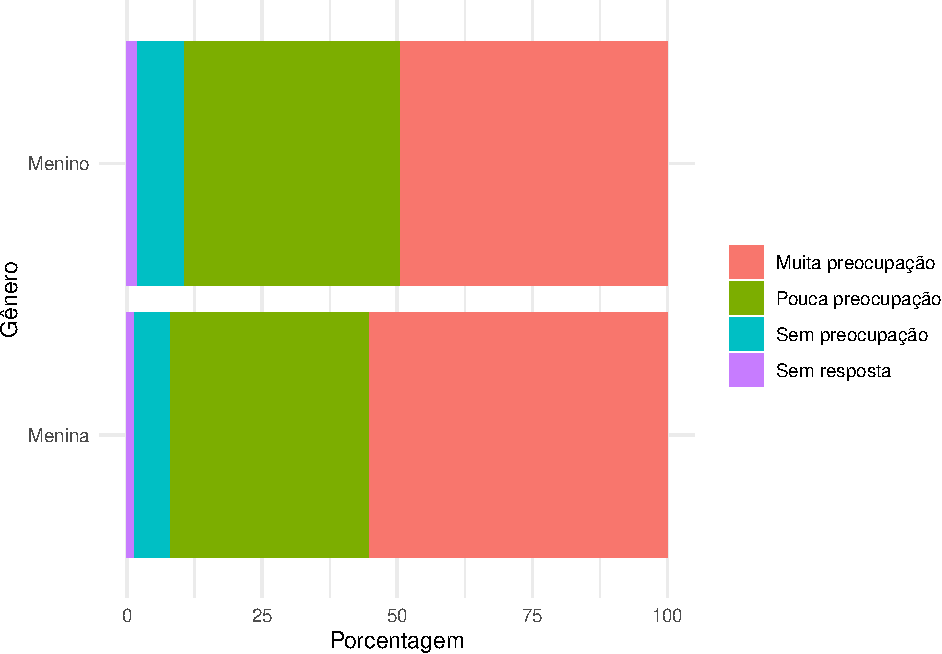
\includegraphics[width=0.75\linewidth]{relatorio_covid19_files/figure-latex/unnamed-chunk-201-1} \end{center}

\hypertarget{teste-qui-quadrado-18}{%
\paragraph{Teste qui-quadrado}\label{teste-qui-quadrado-18}}

Apenas seis crianças se identificaram com o gênero \emph{outros} e foram removidas na análise estatística.

Como o valor-p é igual ou maior que 0.01 (nível de significância), não rejeitamos a hipótese nula e não temos evidência estatística que as duas variáveis estão associadas.

\begin{longtable}[]{@{}ccc@{}}
\caption{\label{tab:unnamed-chunk-203}Teste qui-quadrado entre Gênero e Q17.}\tabularnewline
\toprule
Estatística & Graus de liberdade & Valor-p\tabularnewline
\midrule
\endfirsthead
\toprule
Estatística & Graus de liberdade & Valor-p\tabularnewline
\midrule
\endhead
4,24 & 3 & 0,24\tabularnewline
\bottomrule
\end{longtable}

\cleardoublepage

\hypertarget{medidas-de-resumo-q17-por-guxeanero}{%
\paragraph{Medidas de Resumo Q17 por Gênero}\label{medidas-de-resumo-q17-por-guxeanero}}

Apenas seis crianças se identificaram com o gênero \emph{outros} e foram removidas na análise estatística.

\begin{longtable}[]{@{}cccccc@{}}
\caption{\label{tab:unnamed-chunk-204}Medidas de resumo de Q17 por Gênero.}\tabularnewline
\toprule
Q17 & Média & Desvio Padrão & Mediana & 1 Quartil & 3 Quartil\tabularnewline
\midrule
\endfirsthead
\toprule
Q17 & Média & Desvio Padrão & Mediana & 1 Quartil & 3 Quartil\tabularnewline
\midrule
\endhead
Menina & 1,51 & 0,64 & 2 & 1 & 2\tabularnewline
Menino & 1,44 & 0,68 & 2 & 1 & 2\tabularnewline
\bottomrule
\end{longtable}

\hypertarget{boxplot-de-q17-por-guxeanero}{%
\paragraph{Boxplot de Q17 por Gênero}\label{boxplot-de-q17-por-guxeanero}}

Apenas seis crianças se identificaram com o gênero \emph{outros} e foram removidas na análise estatística.

\begin{center}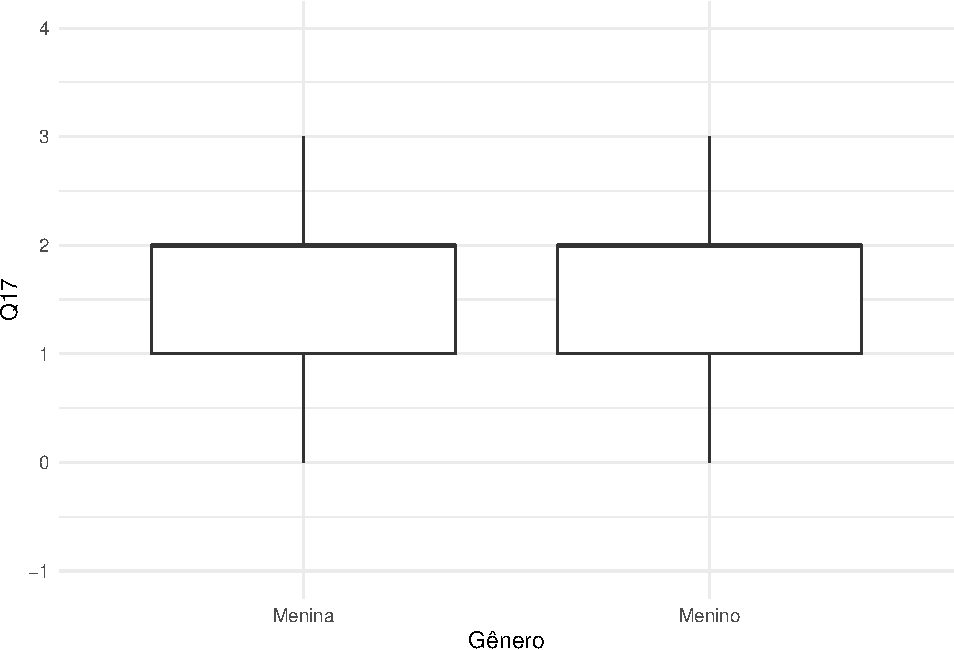
\includegraphics[width=0.75\linewidth]{relatorio_covid19_files/figure-latex/unnamed-chunk-205-1} \end{center}

\hypertarget{teste-de-kruskal-wallis-de-q17-por-guxeanero}{%
\paragraph{Teste de Kruskal-Wallis de Q17 por Gênero}\label{teste-de-kruskal-wallis-de-q17-por-guxeanero}}

Apenas seis crianças se identificaram com o gênero \emph{outros} e foram removidas na análise estatística.

Como o valor-p é maior ou igual a 0.01 (nível de significância), não rejeitamos a hipótese nula e as medianas de Q17 entre meninos e meninas são iguais.

\begin{longtable}[]{@{}ccc@{}}
\caption{\label{tab:unnamed-chunk-207}Valores-p para comparação múltipla de medianas: Q17 e Gênero.}\tabularnewline
\toprule
Estatística & Parâmetro & valor p\tabularnewline
\midrule
\endfirsthead
\toprule
Estatística & Parâmetro & valor p\tabularnewline
\midrule
\endhead
2,94 & 1 & 0,09\tabularnewline
\bottomrule
\end{longtable}

\hypertarget{teste-de-nemeyi-de-q17-por-guxeanero}{%
\paragraph{Teste de Nemeyi de Q17 por Gênero}\label{teste-de-nemeyi-de-q17-por-guxeanero}}

Apenas seis crianças se identificaram com o gênero \emph{outros} e foram removidas na análise estatística.

Como os valores-p são iguais ou maiores que 0.01 (nível de significância), não rejeitamos a hipótese nula e as medianas de Q17 entre meninos e meninas são iguais.

\begin{longtable}[]{@{}lc@{}}
\caption{\label{tab:unnamed-chunk-209}valores-p para o teste de comparação múltipla de Nemeyi de Q17 por Gênero.}\tabularnewline
\toprule
& Menina\tabularnewline
\midrule
\endfirsthead
\toprule
& Menina\tabularnewline
\midrule
\endhead
Menino & 0,13\tabularnewline
\bottomrule
\end{longtable}

\cleardoublepage

\hypertarget{tabela-de-continguxeancia-idade-e-q17}{%
\paragraph{Tabela de contingência: Idade e Q17}\label{tabela-de-continguxeancia-idade-e-q17}}

\begin{longtable}[]{@{}ccccc@{}}
\caption{\label{tab:unnamed-chunk-210}Tabela de contingência: Idade e Q17.}\tabularnewline
\toprule
Idade & Muita preocupação & Pouca preocupação & Sem preocupação & Sem resposta\tabularnewline
\midrule
\endfirsthead
\toprule
Idade & Muita preocupação & Pouca preocupação & Sem preocupação & Sem resposta\tabularnewline
\midrule
\endhead
8 & 92 & 87 & 12 & 4\tabularnewline
9 & 107 & 63 & 14 & 2\tabularnewline
10 & 143 & 81 & 20 & 6\tabularnewline
11 & 120 & 101 & 17 & 2\tabularnewline
12 & 89 & 70 & 18 & 2\tabularnewline
\bottomrule
\end{longtable}

\hypertarget{gruxe1fico-de-barras-idade-e-q17}{%
\paragraph{Gráfico de barras: Idade e Q17}\label{gruxe1fico-de-barras-idade-e-q17}}

\begin{center}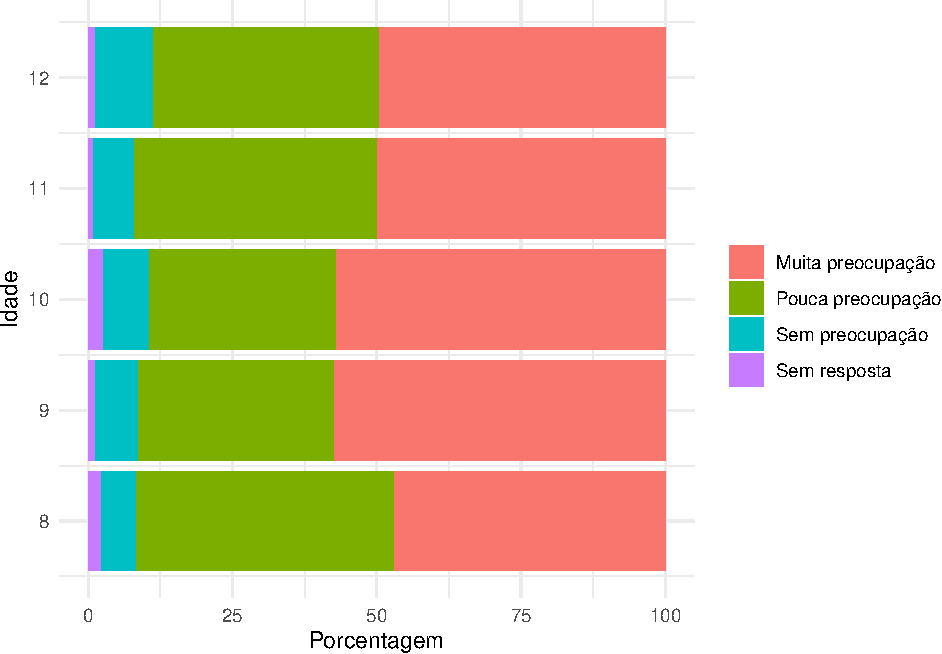
\includegraphics[width=0.75\linewidth]{relatorio_covid19_files/figure-latex/unnamed-chunk-211-1} \end{center}

\hypertarget{teste-qui-quadrado-19}{%
\paragraph{Teste qui-quadrado}\label{teste-qui-quadrado-19}}

Como o valor-p é igual ou maior que 0.01 (nível de significância), não rejeitamos a hipótese nula e não temos evidência estatística que as duas variáveis estão associadas.

\begin{longtable}[]{@{}ccc@{}}
\caption{\label{tab:unnamed-chunk-213}Teste qui-quadrado entre Idade e Q17.}\tabularnewline
\toprule
Estatística & Graus de liberdade & Valor-p\tabularnewline
\midrule
\endfirsthead
\toprule
Estatística & Graus de liberdade & Valor-p\tabularnewline
\midrule
\endhead
14,59 & 12 & 0,26\tabularnewline
\bottomrule
\end{longtable}

\cleardoublepage

\hypertarget{medidas-de-resumo-q17-por-idade}{%
\paragraph{Medidas de Resumo Q17 por Idade}\label{medidas-de-resumo-q17-por-idade}}

\begin{longtable}[]{@{}cccccc@{}}
\caption{\label{tab:unnamed-chunk-214}Medidas de resumo de Q17 por Idade.}\tabularnewline
\toprule
Q17 & Média & Desvio Padrão & Mediana & 1 Quartil & 3 Quartil\tabularnewline
\midrule
\endfirsthead
\toprule
Q17 & Média & Desvio Padrão & Mediana & 1 Quartil & 3 Quartil\tabularnewline
\midrule
\endhead
8 & 1,45 & 0,64 & 1 & 1 & 2\tabularnewline
9 & 1,52 & 0,65 & 2 & 1 & 2\tabularnewline
10 & 1,54 & 0,68 & 2 & 1 & 2\tabularnewline
11 & 1,45 & 0,64 & 2 & 1 & 2\tabularnewline
12 & 1,42 & 0,69 & 2 & 1 & 2\tabularnewline
\bottomrule
\end{longtable}

\hypertarget{boxplot-de-q17-por-idade}{%
\paragraph{Boxplot de Q17 por Idade}\label{boxplot-de-q17-por-idade}}

\begin{center}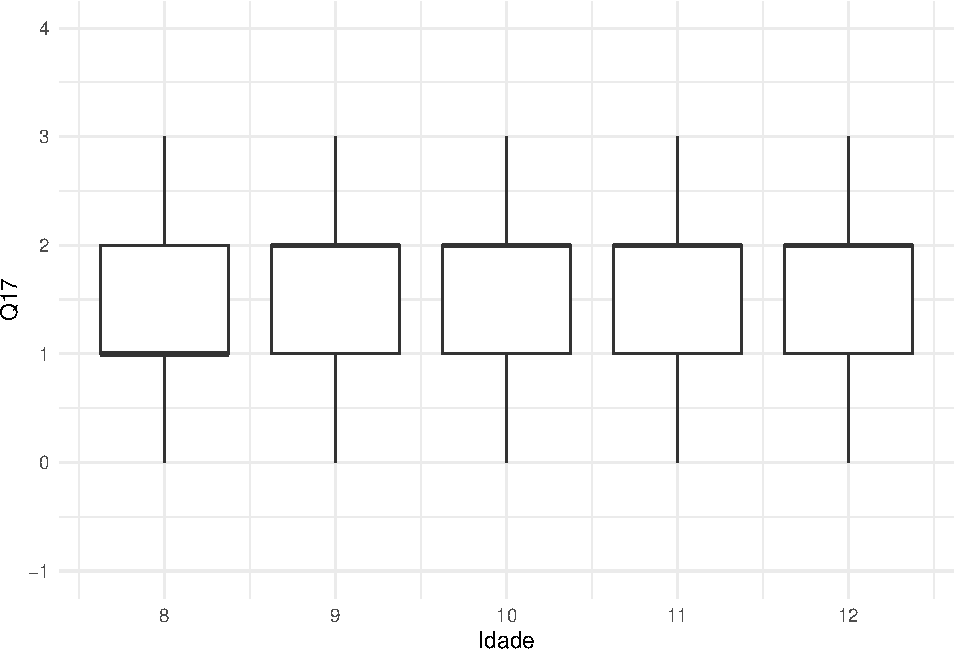
\includegraphics[width=0.75\linewidth]{relatorio_covid19_files/figure-latex/unnamed-chunk-215-1} \end{center}

\hypertarget{teste-de-kruskal-wallis-de-q17-por-idade}{%
\paragraph{Teste de Kruskal-Wallis de Q17 por Idade}\label{teste-de-kruskal-wallis-de-q17-por-idade}}

Como o valor-p é maior ou igual a 0.01 (nível de significância), não rejeitamos a hipótese nula e as medianas de Q17 entre as idades são iguais.

\begin{longtable}[]{@{}ccc@{}}
\caption{\label{tab:unnamed-chunk-217}Valores-p para comparação múltipla de medianas: Q17 e Idade.}\tabularnewline
\toprule
Estatística & Parâmetro & valor p\tabularnewline
\midrule
\endfirsthead
\toprule
Estatística & Parâmetro & valor p\tabularnewline
\midrule
\endhead
6,65 & 4 & 0,16\tabularnewline
\bottomrule
\end{longtable}

\hypertarget{teste-de-nemeyi-de-q17-por-idade}{%
\paragraph{Teste de Nemeyi de Q17 por Idade}\label{teste-de-nemeyi-de-q17-por-idade}}

Como os valores-p são iguais ou maiores que 0.01 (nível de significância), não rejeitamos a hipótese nula e as medianas de Q17 entre pares de crianças de diferentes idades são todas iguais.

\begin{longtable}[]{@{}lcccc@{}}
\caption{\label{tab:unnamed-chunk-219}Teste de Nemeyi de Q17 por Idade.}\tabularnewline
\toprule
& 8 & 9 & 10 & 11\tabularnewline
\midrule
\endfirsthead
\toprule
& 8 & 9 & 10 & 11\tabularnewline
\midrule
\endhead
9 & 0,73 & & &\tabularnewline
10 & 0,51 & 1,00 & &\tabularnewline
11 & 1,00 & 0,73 & 0,49 &\tabularnewline
12 & 1,00 & 0,66 & 0,44 & 1\tabularnewline
\bottomrule
\end{longtable}

\cleardoublepage

\hypertarget{tabela-de-continguxeancia-rauxe7a-e-q17}{%
\paragraph{Tabela de contingência: Raça e Q17}\label{tabela-de-continguxeancia-rauxe7a-e-q17}}

\begin{longtable}[]{@{}ccccc@{}}
\caption{\label{tab:unnamed-chunk-220}Tabela de contingência: Raça e Q17.}\tabularnewline
\toprule
Raça & Muita preocupação & Pouca preocupação & Sem resposta & Sem preocupação\tabularnewline
\midrule
\endfirsthead
\toprule
Raça & Muita preocupação & Pouca preocupação & Sem resposta & Sem preocupação\tabularnewline
\midrule
\endhead
Amarela & 9 & 8 & 2 &\tabularnewline
Branca & 107 & 86 & 1 & 19\tabularnewline
Indígena & 9 & 10 & & 2\tabularnewline
Negra & 399 & 281 & 13 & 56\tabularnewline
Outros & 11 & 5 & &\tabularnewline
Sem resposta & 16 & 12 & & 4\tabularnewline
\bottomrule
\end{longtable}

\hypertarget{gruxe1fico-de-barras-rauxe7a-e-q17}{%
\paragraph{Gráfico de barras: Raça e Q17}\label{gruxe1fico-de-barras-rauxe7a-e-q17}}

\begin{center}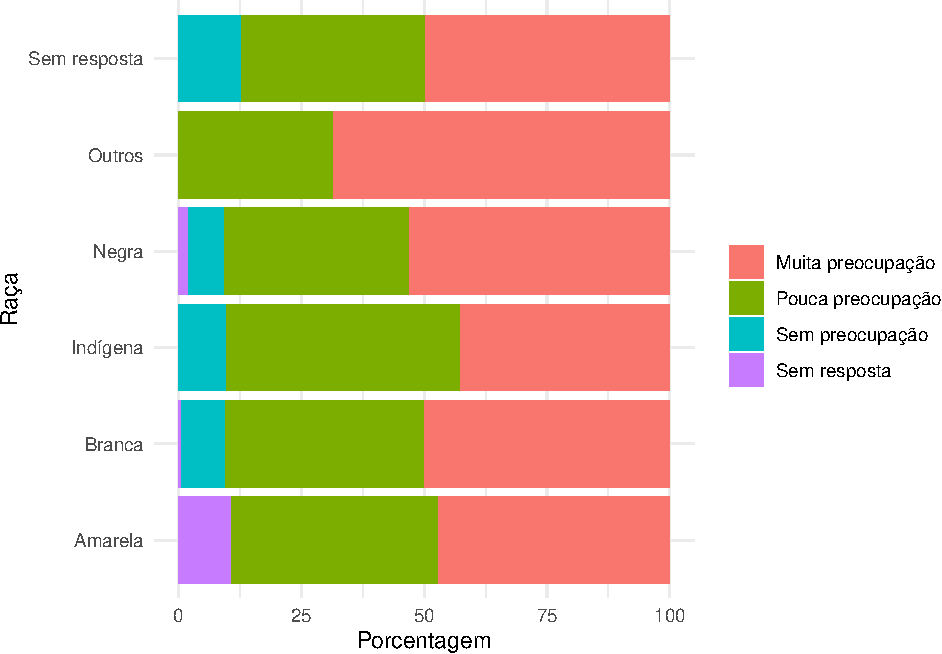
\includegraphics[width=0.75\linewidth]{relatorio_covid19_files/figure-latex/unnamed-chunk-221-1} \end{center}

\hypertarget{teste-qui-quadrado-20}{%
\paragraph{Teste qui-quadrado}\label{teste-qui-quadrado-20}}

Como o valor-p é igual ou maior que 0.01 (nível de significância), não rejeitamos a hipótese nula e não temos evidência estatística que as duas variáveis estão associadas.

\begin{longtable}[]{@{}ccc@{}}
\caption{\label{tab:unnamed-chunk-223}Teste qui-quadrado entre raca e Q17.}\tabularnewline
\toprule
Estatística & Graus de liberdade & Valor-p\tabularnewline
\midrule
\endfirsthead
\toprule
Estatística & Graus de liberdade & Valor-p\tabularnewline
\midrule
\endhead
19,85 & 15 & 0,18\tabularnewline
\bottomrule
\end{longtable}

\cleardoublepage

\hypertarget{medidas-de-resumo-q17-por-rauxe7a}{%
\paragraph{Medidas de Resumo Q17 por Raça}\label{medidas-de-resumo-q17-por-rauxe7a}}

\begin{longtable}[]{@{}cccccc@{}}
\caption{\label{tab:unnamed-chunk-224}Medidas de resumo de Q17 por raca.}\tabularnewline
\toprule
Q17 & Média & Desvio Padrão & Mediana & 1 Quartil & 3 Quartil\tabularnewline
\midrule
\endfirsthead
\toprule
Q17 & Média & Desvio Padrão & Mediana & 1 Quartil & 3 Quartil\tabularnewline
\midrule
\endhead
Amarela & 1,68 & 0,67 & 2,0 & 1 & 2\tabularnewline
Branca & 1,42 & 0,66 & 2,0 & 1 & 2\tabularnewline
Indígena & 1,33 & 0,66 & 1,0 & 1 & 2\tabularnewline
Negra & 1,49 & 0,66 & 2,0 & 1 & 2\tabularnewline
Outros & 1,69 & 0,48 & 2,0 & 1 & 2\tabularnewline
Sem resposta & 1,38 & 0,71 & 1,5 & 1 & 2\tabularnewline
\bottomrule
\end{longtable}

\hypertarget{boxplot-de-q17-por-rauxe7a}{%
\paragraph{Boxplot de Q17 por Raça}\label{boxplot-de-q17-por-rauxe7a}}

\begin{center}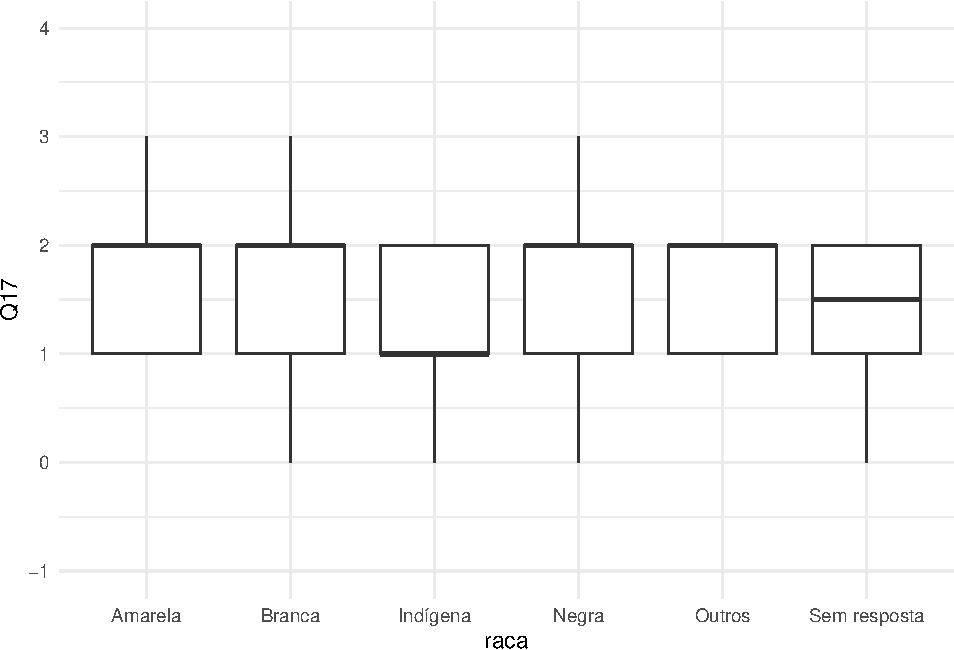
\includegraphics[width=0.75\linewidth]{relatorio_covid19_files/figure-latex/unnamed-chunk-225-1} \end{center}

\hypertarget{teste-de-kruskal-wallis-de-q17-por-rauxe7a}{%
\paragraph{Teste de Kruskal-Wallis de Q17 por Raça}\label{teste-de-kruskal-wallis-de-q17-por-rauxe7a}}

Como o valor-p é maior ou igual a 0.01 (nível de significância), não rejeitamos a hipótese nula e as medianas de Q17 entre raças são todas iguais.

\begin{longtable}[]{@{}ccc@{}}
\caption{\label{tab:unnamed-chunk-227}Valores-p para comparação múltipla de medianas: Q17 e Raça.}\tabularnewline
\toprule
Estatística & Parâmetro & valor p\tabularnewline
\midrule
\endfirsthead
\toprule
Estatística & Parâmetro & valor p\tabularnewline
\midrule
\endhead
5,92 & 5 & 0,31\tabularnewline
\bottomrule
\end{longtable}

\hypertarget{teste-de-nemeyi-de-q17-por-rauxe7a}{%
\paragraph{Teste de Nemeyi de Q17 por Raça}\label{teste-de-nemeyi-de-q17-por-rauxe7a}}

Como os valores-p são iguais ou maiores que 0.01 (nível de significância), não rejeitamos a hipótese nula e as medianas de Q17 entre as raças são iguais.

\begin{longtable}[]{@{}lccccc@{}}
\caption{\label{tab:unnamed-chunk-229}Valores-p para o teste de Nemeyi de Q17 por Raça.}\tabularnewline
\toprule
& Amarela & Branca & Indígena & Negra & Outros\tabularnewline
\midrule
\endfirsthead
\toprule
& Amarela & Branca & Indígena & Negra & Outros\tabularnewline
\midrule
\endhead
Branca & 0,86 & & & &\tabularnewline
Indígena & 0,79 & 0,99 & & &\tabularnewline
Negra & 0,97 & 0,85 & 0,91 & &\tabularnewline
Outros & 1,00 & 0,76 & 0,69 & 0,91 &\tabularnewline
Sem resposta & 0,88 & 1,00 & 1,00 & 0,98 & 0,79\tabularnewline
\bottomrule
\end{longtable}

\cleardoublepage

\hypertarget{tabela-de-continguxeancia-tipo-de-escola-e-q17}{%
\paragraph{Tabela de contingência: Tipo de escola e Q17}\label{tabela-de-continguxeancia-tipo-de-escola-e-q17}}

Apenas sete crianças não estavam matriculadas na escola, e foram retiradas da análise para facilitar a análise de \emph{tipo de escola}.

\begin{longtable}[]{@{}ccccc@{}}
\caption{\label{tab:unnamed-chunk-230}Tabela de contingência: Tipo de escola e Q17.}\tabularnewline
\toprule
\begin{minipage}[b]{0.16\columnwidth}\centering
Tipo de Escola\strut
\end{minipage} & \begin{minipage}[b]{0.19\columnwidth}\centering
Muita preocupação\strut
\end{minipage} & \begin{minipage}[b]{0.19\columnwidth}\centering
Pouca preocupação\strut
\end{minipage} & \begin{minipage}[b]{0.17\columnwidth}\centering
Sem preocupação\strut
\end{minipage} & \begin{minipage}[b]{0.14\columnwidth}\centering
Sem resposta\strut
\end{minipage}\tabularnewline
\midrule
\endfirsthead
\toprule
\begin{minipage}[b]{0.16\columnwidth}\centering
Tipo de Escola\strut
\end{minipage} & \begin{minipage}[b]{0.19\columnwidth}\centering
Muita preocupação\strut
\end{minipage} & \begin{minipage}[b]{0.19\columnwidth}\centering
Pouca preocupação\strut
\end{minipage} & \begin{minipage}[b]{0.17\columnwidth}\centering
Sem preocupação\strut
\end{minipage} & \begin{minipage}[b]{0.14\columnwidth}\centering
Sem resposta\strut
\end{minipage}\tabularnewline
\midrule
\endhead
\begin{minipage}[t]{0.16\columnwidth}\centering
Particular\strut
\end{minipage} & \begin{minipage}[t]{0.19\columnwidth}\centering
303\strut
\end{minipage} & \begin{minipage}[t]{0.19\columnwidth}\centering
234\strut
\end{minipage} & \begin{minipage}[t]{0.17\columnwidth}\centering
44\strut
\end{minipage} & \begin{minipage}[t]{0.14\columnwidth}\centering
9\strut
\end{minipage}\tabularnewline
\begin{minipage}[t]{0.16\columnwidth}\centering
Pública\strut
\end{minipage} & \begin{minipage}[t]{0.19\columnwidth}\centering
247\strut
\end{minipage} & \begin{minipage}[t]{0.19\columnwidth}\centering
164\strut
\end{minipage} & \begin{minipage}[t]{0.17\columnwidth}\centering
35\strut
\end{minipage} & \begin{minipage}[t]{0.14\columnwidth}\centering
7\strut
\end{minipage}\tabularnewline
\bottomrule
\end{longtable}

\hypertarget{gruxe1fico-de-barras-tipo-de-escola-e-q17}{%
\paragraph{Gráfico de barras: Tipo de escola e Q17}\label{gruxe1fico-de-barras-tipo-de-escola-e-q17}}

Apenas sete crianças não estavam matriculadas na escola, e foram retiradas da análise para facilitar a análise de \emph{tipo de escola}.

\begin{center}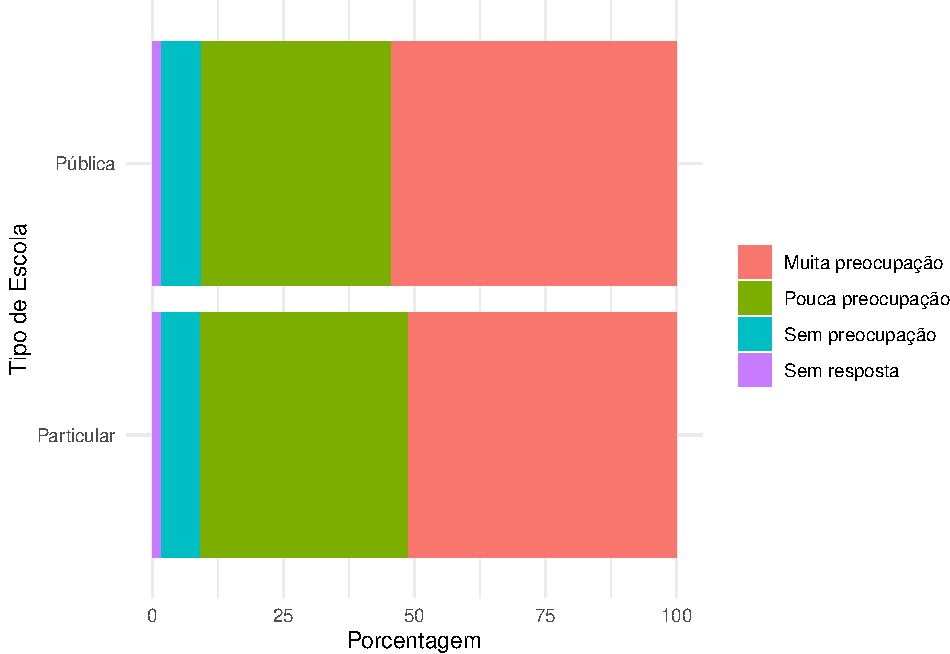
\includegraphics[width=0.75\linewidth]{relatorio_covid19_files/figure-latex/unnamed-chunk-231-1} \end{center}

\hypertarget{teste-qui-quadrado-21}{%
\paragraph{Teste qui-quadrado}\label{teste-qui-quadrado-21}}

Apenas sete crianças não estavam matriculadas na escola, e foram retiradas da análise para facilitar a análise de \emph{tipo de escola}.

Como o valor-p é igual ou maior que 0.01 (nível de significância), não rejeitamos a hipótese nula e não temos evidência estatística que as duas variáveis estão associadas.

\begin{longtable}[]{@{}ccc@{}}
\caption{\label{tab:unnamed-chunk-233}Teste qui-quadrado entre Escola e Q17.}\tabularnewline
\toprule
Estatística & Graus de liberdade & Valor-p\tabularnewline
\midrule
\endfirsthead
\toprule
Estatística & Graus de liberdade & Valor-p\tabularnewline
\midrule
\endhead
1,32 & 3 & 0,73\tabularnewline
\bottomrule
\end{longtable}

\cleardoublepage

\hypertarget{medidas-de-resumo-q17-por-tipo-de-escola}{%
\paragraph{Medidas de Resumo Q17 por Tipo de escola}\label{medidas-de-resumo-q17-por-tipo-de-escola}}

Apenas sete crianças não estavam matriculadas na escola, e foram retiradas da análise para facilitar a análise de \emph{tipo de escola}.

\begin{longtable}[]{@{}cccccc@{}}
\caption{\label{tab:unnamed-chunk-234}Medidas de resumo de Q17 por Escola.}\tabularnewline
\toprule
Q17 & Média & Desvio Padrão & Mediana & 1 Quartil & 3 Quartil\tabularnewline
\midrule
\endfirsthead
\toprule
Q17 & Média & Desvio Padrão & Mediana & 1 Quartil & 3 Quartil\tabularnewline
\midrule
\endhead
Particular & 1,47 & 0,66 & 2 & 1 & 2\tabularnewline
Pública & 1,50 & 0,66 & 2 & 1 & 2\tabularnewline
\bottomrule
\end{longtable}

\hypertarget{boxplot-de-q17-por-tipo-de-escola}{%
\paragraph{Boxplot de Q17 por Tipo de escola}\label{boxplot-de-q17-por-tipo-de-escola}}

Apenas sete crianças não estavam matriculadas na escola, e foram retiradas da análise para facilitar a análise de \emph{tipo de escola}.

\begin{center}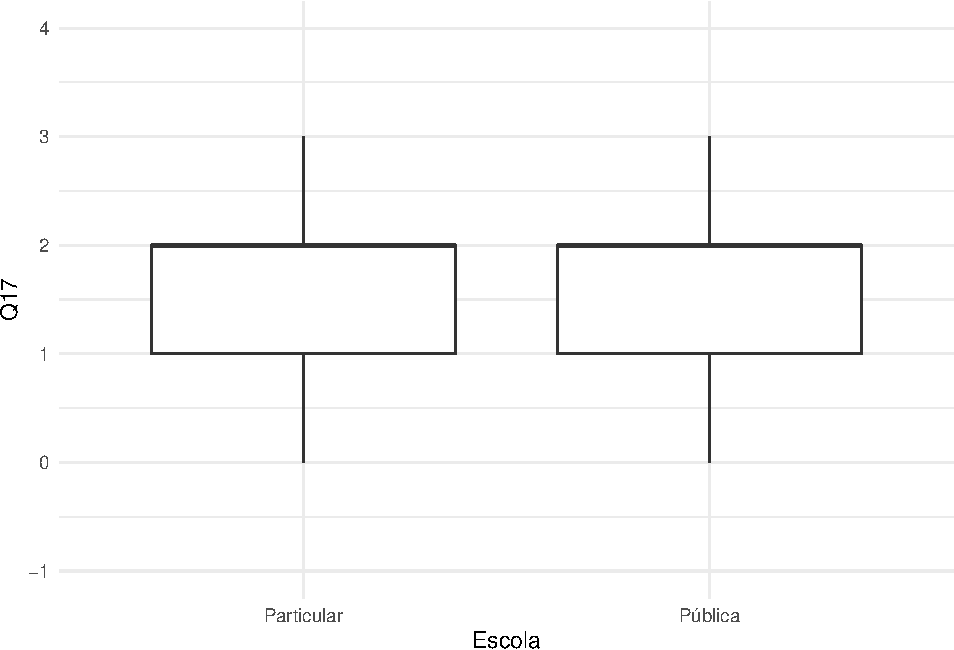
\includegraphics[width=0.75\linewidth]{relatorio_covid19_files/figure-latex/unnamed-chunk-235-1} \end{center}

\hypertarget{teste-de-kruskal-wallis-de-q17-por-tipo-de-escola}{%
\paragraph{Teste de Kruskal-Wallis de Q17 por Tipo de escola}\label{teste-de-kruskal-wallis-de-q17-por-tipo-de-escola}}

Apenas sete crianças não estavam matriculadas na escola, e foram retiradas da análise para facilitar a análise de \emph{tipo de escola}.

Como o valor-p é maior ou igual a 0.01 (nível de significância), não rejeitamos a hipótese nula e as medianas de Q17 entre tipos de escola são iguais.

\begin{longtable}[]{@{}ccc@{}}
\caption{\label{tab:unnamed-chunk-237}Valores-p para comparação múltipla de medianas: Q17 e Tipo de escola.}\tabularnewline
\toprule
Estatística & Parâmetro & valor p\tabularnewline
\midrule
\endfirsthead
\toprule
Estatística & Parâmetro & valor p\tabularnewline
\midrule
\endhead
0,75 & 1 & 0,39\tabularnewline
\bottomrule
\end{longtable}

\hypertarget{teste-de-nemeyi-de-q17-por-tipo-de-escola}{%
\paragraph{Teste de Nemeyi de Q17 por Tipo de escola}\label{teste-de-nemeyi-de-q17-por-tipo-de-escola}}

Apenas sete crianças não estavam matriculadas na escola, e foram retiradas da análise para facilitar a análise de \emph{tipo de escola}.

Como os valores-p são iguais ou maiores que 0.01 (nível de significância), não rejeitamos a hipótese nula e as medianas de Q17 entre tipos de escola são iguais.

\begin{longtable}[]{@{}lc@{}}
\caption{\label{tab:unnamed-chunk-239}Teste de Nemeyi de Q17 por Escola.}\tabularnewline
\toprule
& Particular\tabularnewline
\midrule
\endfirsthead
\toprule
& Particular\tabularnewline
\midrule
\endhead
Pública & 0,44\tabularnewline
\bottomrule
\end{longtable}

\cleardoublepage

\hypertarget{q18}{%
\subsection{Q18}\label{q18}}

A variável Q18 corresponde ao campo de númeo 13 com enunciado \textbf{O quanto você está preocupado hoje com as questões abaixo} no quesito:

\begin{itemize}
\tightlist
\item
  \emph{Que eu fique doente com o coronavírus}
\end{itemize}

\hypertarget{anuxe1lise-descritiva-para-q18}{%
\subsubsection{Análise descritiva para Q18}\label{anuxe1lise-descritiva-para-q18}}

\hypertarget{gruxe1fico-de-barras-q18}{%
\paragraph{Gráfico de barras: Q18}\label{gruxe1fico-de-barras-q18}}

\begin{center}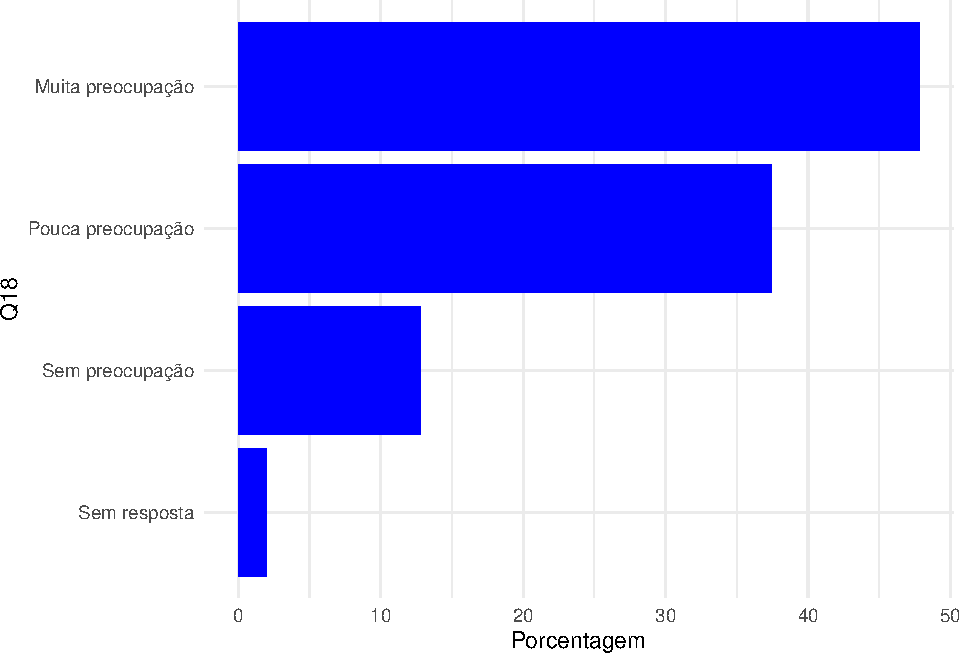
\includegraphics[width=0.75\linewidth]{relatorio_covid19_files/figure-latex/unnamed-chunk-246-1} \end{center}

\hypertarget{tabela-de-distribuiuxe7uxe3o-q18}{%
\paragraph{Tabela de distribuição: Q18}\label{tabela-de-distribuiuxe7uxe3o-q18}}

\begin{longtable}[]{@{}cccc@{}}
\caption{\label{tab:unnamed-chunk-247}Que eu fique doente com o coronavírus}\tabularnewline
\toprule
Q18 & Frequência & Frequência relativa & Porcentagem\tabularnewline
\midrule
\endfirsthead
\toprule
Q18 & Frequência & Frequência relativa & Porcentagem\tabularnewline
\midrule
\endhead
Muita preocupação & 502 & 0,48 & 47,81\tabularnewline
Pouca preocupação & 393 & 0,37 & 37,43\tabularnewline
Sem preocupação & 134 & 0,13 & 12,76\tabularnewline
Sem resposta & 21 & 0,02 & 2,00\tabularnewline
\bottomrule
\end{longtable}

\hypertarget{medidas-de-resumo-q18}{%
\paragraph{Medidas de resumo: Q18}\label{medidas-de-resumo-q18}}

\begin{longtable}[]{@{}ccccc@{}}
\caption{\label{tab:unnamed-chunk-248}Resumos para variável Q18.}\tabularnewline
\toprule
Média & Desvio Padrão & Mediana & 1Qua & 3Qua\tabularnewline
\midrule
\endfirsthead
\toprule
Média & Desvio Padrão & Mediana & 1Qua & 3Qua\tabularnewline
\midrule
\endhead
1,39 & 0,73 & 1 & 1 & 2\tabularnewline
\bottomrule
\end{longtable}

\cleardoublepage

\hypertarget{anuxe1lise-bidimensional-q18}{%
\subsubsection{Análise bidimensional Q18}\label{anuxe1lise-bidimensional-q18}}

\hypertarget{tabela-de-continguxeancia-cidade-e-q18}{%
\paragraph{Tabela de contingência: Cidade e Q18}\label{tabela-de-continguxeancia-cidade-e-q18}}

\begin{longtable}[]{@{}ccccc@{}}
\caption{\label{tab:unnamed-chunk-249}Tabela de contingência: Cidade e Q18.}\tabularnewline
\toprule
Cidade & Muita preocupação & Pouca preocupação & Sem preocupação & Sem resposta\tabularnewline
\midrule
\endfirsthead
\toprule
Cidade & Muita preocupação & Pouca preocupação & Sem preocupação & Sem resposta\tabularnewline
\midrule
\endhead
Camaçari & 72 & 77 & 40 & 8\tabularnewline
Candeias & 12 & 15 & 9 & 2\tabularnewline
Lauro de Freitas & 11 & 26 & 23 & 1\tabularnewline
Outros & 23 & 41 & 19 &\tabularnewline
Pojuca & 25 & 27 & 10 & 2\tabularnewline
Salvador & 113 & 225 & 217 & 18\tabularnewline
Simões Filho & 9 & 17 & 7 & 1\tabularnewline
\bottomrule
\end{longtable}

\hypertarget{gruxe1fico-de-barras-cidade-e-q18}{%
\paragraph{Gráfico de barras: Cidade e Q18}\label{gruxe1fico-de-barras-cidade-e-q18}}

\begin{center}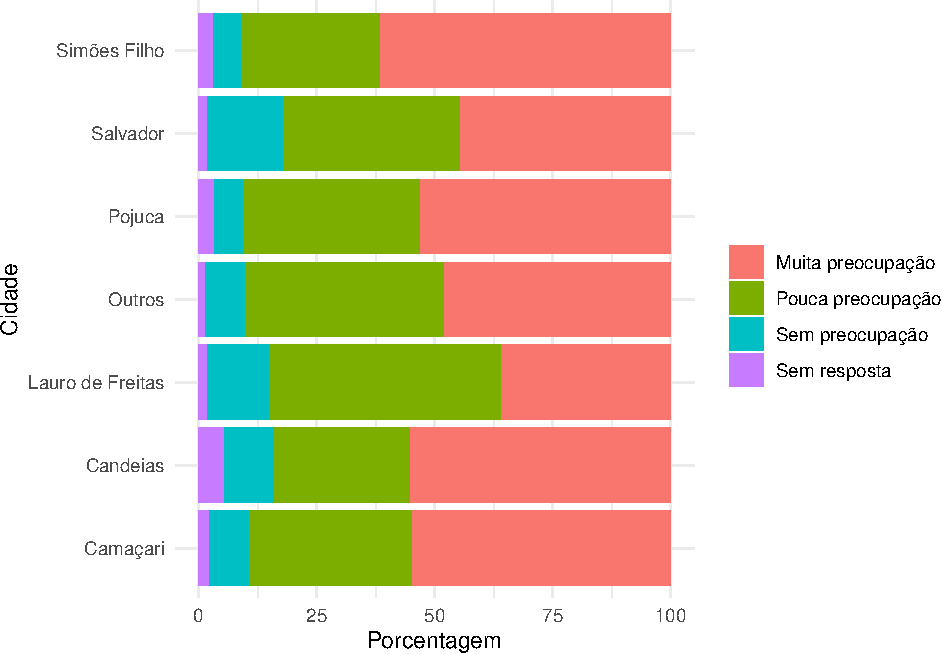
\includegraphics[width=0.75\linewidth]{relatorio_covid19_files/figure-latex/unnamed-chunk-250-1} \end{center}

\hypertarget{teste-qui-quadrado-22}{%
\paragraph{Teste qui-quadrado}\label{teste-qui-quadrado-22}}

Como o valor-p é igual igual ou maior que 0.01 (nível de significância), não rejeitamos a hipótese nula e não temos evidência estatística que as duas variáveis estão associadas.

\begin{longtable}[]{@{}ccc@{}}
\caption{\label{tab:unnamed-chunk-252}Teste qui-quadrado entre Cidade e Q18.}\tabularnewline
\toprule
Estatística & Graus de liberdade & Valor-p\tabularnewline
\midrule
\endfirsthead
\toprule
Estatística & Graus de liberdade & Valor-p\tabularnewline
\midrule
\endhead
27,02 & 18 & 0,08\tabularnewline
\bottomrule
\end{longtable}

\cleardoublepage

\hypertarget{medidas-de-resumo-q18-por-cidade}{%
\paragraph{Medidas de Resumo Q18 por Cidade}\label{medidas-de-resumo-q18-por-cidade}}

\begin{longtable}[]{@{}cccccc@{}}
\caption{\label{tab:unnamed-chunk-253}Medidas de resumo de Q18 por Cidade.}\tabularnewline
\toprule
Q18 & Média & Desvio Padrão & Mediana & 1 Quartil & 3 Quartil\tabularnewline
\midrule
\endfirsthead
\toprule
Q18 & Média & Desvio Padrão & Mediana & 1 Quartil & 3 Quartil\tabularnewline
\midrule
\endhead
Camaçari & 1,50 & 0,68 & 2 & 1 & 2\tabularnewline
Candeias & 1,55 & 0,76 & 2 & 1 & 2\tabularnewline
Lauro de Freitas & 1,26 & 0,70 & 1 & 1 & 2\tabularnewline
Outros & 1,42 & 0,66 & 1 & 1 & 2\tabularnewline
Pojuca & 1,53 & 0,67 & 2 & 1 & 2\tabularnewline
Salvador & 1,32 & 0,76 & 1 & 1 & 2\tabularnewline
Simões Filho & 1,62 & 0,65 & 2 & 1 & 2\tabularnewline
\bottomrule
\end{longtable}

\hypertarget{boxplot-de-q18-por-cidade}{%
\paragraph{Boxplot de Q18 por Cidade}\label{boxplot-de-q18-por-cidade}}

\begin{center}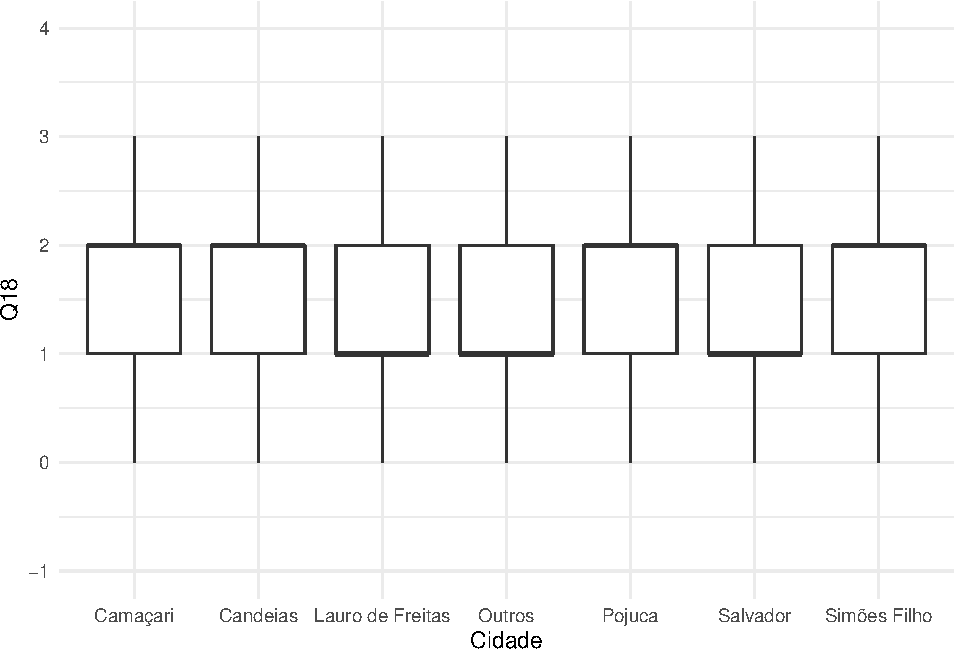
\includegraphics[width=0.75\linewidth]{relatorio_covid19_files/figure-latex/unnamed-chunk-254-1} \end{center}

\hypertarget{teste-de-kruskal-wallis-de-q18-por-cidade}{%
\paragraph{Teste de Kruskal-Wallis de Q18 por Cidade}\label{teste-de-kruskal-wallis-de-q18-por-cidade}}

Como o valor-p é menor que 0.01 (nível de significância), rejeitamos a hipótese nula e as medianas de Q18 entre as crianças de diversas cidades não são todas iguais.

\begin{longtable}[]{@{}ccc@{}}
\caption{\label{tab:unnamed-chunk-256}Valor-p para o teste de Kruskal-Wallis: Q18 e Cidade.}\tabularnewline
\toprule
Estatística & Parâmetro & valor p\tabularnewline
\midrule
\endfirsthead
\toprule
Estatística & Parâmetro & valor p\tabularnewline
\midrule
\endhead
18,93 & 6 & 0\tabularnewline
\bottomrule
\end{longtable}

\hypertarget{teste-de-nemeyi-de-q18-por-cidade}{%
\paragraph{Teste de Nemeyi de Q18 por Cidade}\label{teste-de-nemeyi-de-q18-por-cidade}}

Como os valores-p são iguais ou maiores que 0.01 (nível de significância), não rejeitamos a hipótese nula e as medianas de Q18 entre as crianças de diversas cidades são iguais.

\begin{longtable}[]{@{}lcccccc@{}}
\caption{\label{tab:unnamed-chunk-258}Valores-p para o teste de comparação múltipla de Nemeyi de Q18 por Cidade.}\tabularnewline
\toprule
& Camaçari & Candeias & Lauro de Freitas & Outros & Pojuca & Salvador\tabularnewline
\midrule
\endfirsthead
\toprule
& Camaçari & Candeias & Lauro de Freitas & Outros & Pojuca & Salvador\tabularnewline
\midrule
\endhead
Candeias & 1,00 & & & & &\tabularnewline
Lauro de Freitas & 0,29 & 0,49 & & & &\tabularnewline
Outros & 0,98 & 0,97 & 0,88 & & &\tabularnewline
Pojuca & 1,00 & 1,00 & 0,46 & 0,98 & &\tabularnewline
Salvador & 0,10 & 0,61 & 0,99 & 0,97 & 0,52 &\tabularnewline
Simões Filho & 0,99 & 1,00 & 0,29 & 0,86 & 1,00 & 0,36\tabularnewline
\bottomrule
\end{longtable}

\cleardoublepage

\hypertarget{tabela-de-continguxeancia-guxeanero-e-q18}{%
\paragraph{Tabela de contingência: Gênero e Q18}\label{tabela-de-continguxeancia-guxeanero-e-q18}}

Apenas seis crianças se identificaram com o gênero \emph{outros} e foram removidas na análise estatística.

\begin{longtable}[]{@{}ccccc@{}}
\caption{\label{tab:unnamed-chunk-259}Tabela de contingência: Gênero e Q18.}\tabularnewline
\toprule
Gênero & Muita preocupação & Pouca preocupação & Sem preocupação & Sem resposta\tabularnewline
\midrule
\endfirsthead
\toprule
Gênero & Muita preocupação & Pouca preocupação & Sem preocupação & Sem resposta\tabularnewline
\midrule
\endhead
Menina & 267 & 189 & 73 & 12\tabularnewline
Menino & 232 & 202 & 60 & 9\tabularnewline
\bottomrule
\end{longtable}

\hypertarget{gruxe1fico-de-barras-guxeanero-e-q18}{%
\paragraph{Gráfico de barras: Gênero e Q18}\label{gruxe1fico-de-barras-guxeanero-e-q18}}

Apenas seis crianças se identificaram com o gênero \emph{outros} e foram removidas na análise estatística.

\begin{center}\includegraphics[width=0.75\linewidth]{relatorio_covid19_files/figure-latex/unnamed-chunk-260-1} \end{center}

\hypertarget{teste-qui-quadrado-23}{%
\paragraph{Teste qui-quadrado}\label{teste-qui-quadrado-23}}

Apenas seis crianças se identificaram com o gênero \emph{outros} e foram removidas na análise estatística.

Como o valor-p é igual ou maior que 0.01 (nível de significância), não rejeitamos a hipótese nula e não temos evidência estatística que as duas variáveis estão associadas.

\begin{longtable}[]{@{}ccc@{}}
\caption{\label{tab:unnamed-chunk-262}Teste qui-quadrado entre Gênero e Q18.}\tabularnewline
\toprule
Estatística & Graus de liberdade & Valor-p\tabularnewline
\midrule
\endfirsthead
\toprule
Estatística & Graus de liberdade & Valor-p\tabularnewline
\midrule
\endhead
3,21 & 3 & 0,36\tabularnewline
\bottomrule
\end{longtable}

\cleardoublepage

\hypertarget{medidas-de-resumo-q18-por-guxeanero}{%
\paragraph{Medidas de Resumo Q18 por Gênero}\label{medidas-de-resumo-q18-por-guxeanero}}

Apenas seis crianças se identificaram com o gênero \emph{outros} e foram removidas na análise estatística.

\begin{longtable}[]{@{}cccccc@{}}
\caption{\label{tab:unnamed-chunk-263}Medidas de resumo de Q18 por Gênero.}\tabularnewline
\toprule
Q18 & Média & Desvio Padrão & Mediana & 1 Quartil & 3 Quartil\tabularnewline
\midrule
\endfirsthead
\toprule
Q18 & Média & Desvio Padrão & Mediana & 1 Quartil & 3 Quartil\tabularnewline
\midrule
\endhead
Menina & 1,40 & 0,75 & 2 & 1 & 2\tabularnewline
Menino & 1,38 & 0,71 & 1 & 1 & 2\tabularnewline
\bottomrule
\end{longtable}

\hypertarget{boxplot-de-q18-por-guxeanero}{%
\paragraph{Boxplot de Q18 por Gênero}\label{boxplot-de-q18-por-guxeanero}}

Apenas seis crianças se identificaram com o gênero \emph{outros} e foram removidas na análise estatística.

\begin{center}\includegraphics[width=0.75\linewidth]{relatorio_covid19_files/figure-latex/unnamed-chunk-264-1} \end{center}

\hypertarget{teste-de-kruskal-wallis-de-q18-por-guxeanero}{%
\paragraph{Teste de Kruskal-Wallis de Q18 por Gênero}\label{teste-de-kruskal-wallis-de-q18-por-guxeanero}}

Apenas seis crianças se identificaram com o gênero \emph{outros} e foram removidas na análise estatística.

Como o valor-p é maior ou igual a 0.01 (nível de significância), não rejeitamos a hipótese nula e as medianas de Q18 entre meninos e meninas são iguais.

\begin{longtable}[]{@{}ccc@{}}
\caption{\label{tab:unnamed-chunk-266}Valores-p para comparação múltipla de medianas: Q18 e Gênero.}\tabularnewline
\toprule
Estatística & Parâmetro & valor p\tabularnewline
\midrule
\endfirsthead
\toprule
Estatística & Parâmetro & valor p\tabularnewline
\midrule
\endhead
0,61 & 1 & 0,44\tabularnewline
\bottomrule
\end{longtable}

\hypertarget{teste-de-nemeyi-de-q18-por-guxeanero}{%
\paragraph{Teste de Nemeyi de Q18 por Gênero}\label{teste-de-nemeyi-de-q18-por-guxeanero}}

Apenas seis crianças se identificaram com o gênero \emph{outros} e foram removidas na análise estatística.

Como os valores-p são iguais ou maiores que 0.01 (nível de significância), não rejeitamos a hipótese nula e as medianas de Q18 entre meninos e meninas são iguais.

\begin{longtable}[]{@{}lc@{}}
\caption{\label{tab:unnamed-chunk-268}valores-p para o teste de comparação múltipla de Nemeyi de Q18 por Gênero.}\tabularnewline
\toprule
& Menina\tabularnewline
\midrule
\endfirsthead
\toprule
& Menina\tabularnewline
\midrule
\endhead
Menino & 0,48\tabularnewline
\bottomrule
\end{longtable}

\cleardoublepage

\hypertarget{tabela-de-continguxeancia-idade-e-q18}{%
\paragraph{Tabela de contingência: Idade e Q18}\label{tabela-de-continguxeancia-idade-e-q18}}

\begin{longtable}[]{@{}ccccc@{}}
\caption{\label{tab:unnamed-chunk-269}Tabela de contingência: Idade e Q18.}\tabularnewline
\toprule
Idade & Muita preocupação & Pouca preocupação & Sem preocupação & Sem resposta\tabularnewline
\midrule
\endfirsthead
\toprule
Idade & Muita preocupação & Pouca preocupação & Sem preocupação & Sem resposta\tabularnewline
\midrule
\endhead
8 & 92 & 81 & 18 & 4\tabularnewline
9 & 100 & 61 & 21 & 4\tabularnewline
10 & 129 & 80 & 34 & 7\tabularnewline
11 & 106 & 100 & 30 & 4\tabularnewline
12 & 75 & 71 & 31 & 2\tabularnewline
\bottomrule
\end{longtable}

\hypertarget{gruxe1fico-de-barras-idade-e-q18}{%
\paragraph{Gráfico de barras: Idade e Q18}\label{gruxe1fico-de-barras-idade-e-q18}}

\begin{center}\includegraphics[width=0.75\linewidth]{relatorio_covid19_files/figure-latex/unnamed-chunk-270-1} \end{center}

\hypertarget{teste-qui-quadrado-24}{%
\paragraph{Teste qui-quadrado}\label{teste-qui-quadrado-24}}

Como o valor-p é igual ou maior que 0.01 (nível de significância), não rejeitamos a hipótese nula e não temos evidência estatística que as duas variáveis estão associadas.

\begin{longtable}[]{@{}ccc@{}}
\caption{\label{tab:unnamed-chunk-272}Teste qui-quadrado entre Idade e Q18.}\tabularnewline
\toprule
Estatística & Graus de liberdade & Valor-p\tabularnewline
\midrule
\endfirsthead
\toprule
Estatística & Graus de liberdade & Valor-p\tabularnewline
\midrule
\endhead
16,36 & 12 & 0,18\tabularnewline
\bottomrule
\end{longtable}

\cleardoublepage

\hypertarget{medidas-de-resumo-q18-por-idade}{%
\paragraph{Medidas de Resumo Q18 por Idade}\label{medidas-de-resumo-q18-por-idade}}

\begin{longtable}[]{@{}cccccc@{}}
\caption{\label{tab:unnamed-chunk-273}Medidas de resumo de Q18 por Idade.}\tabularnewline
\toprule
Q18 & Média & Desvio Padrão & Mediana & 1 Quartil & 3 Quartil\tabularnewline
\midrule
\endfirsthead
\toprule
Q18 & Média & Desvio Padrão & Mediana & 1 Quartil & 3 Quartil\tabularnewline
\midrule
\endhead
8 & 1,42 & 0,69 & 1 & 1 & 2\tabularnewline
9 & 1,47 & 0,72 & 2 & 1 & 2\tabularnewline
10 & 1,44 & 0,76 & 2 & 1 & 2\tabularnewline
11 & 1,35 & 0,72 & 1 & 1 & 2\tabularnewline
12 & 1,27 & 0,75 & 1 & 1 & 2\tabularnewline
\bottomrule
\end{longtable}

\hypertarget{boxplot-de-q18-por-idade}{%
\paragraph{Boxplot de Q18 por Idade}\label{boxplot-de-q18-por-idade}}

\begin{center}\includegraphics[width=0.75\linewidth]{relatorio_covid19_files/figure-latex/unnamed-chunk-274-1} \end{center}

\hypertarget{teste-de-kruskal-wallis-de-q18-por-idade}{%
\paragraph{Teste de Kruskal-Wallis de Q18 por Idade}\label{teste-de-kruskal-wallis-de-q18-por-idade}}

Como o valor-p é maior ou igual a 0.01 (nível de significância), não rejeitamos a hipótese nula e as medianas de Q18 entre as idades são iguais.

\begin{longtable}[]{@{}ccc@{}}
\caption{\label{tab:unnamed-chunk-276}Valores-p para comparação múltipla de medianas: Q18 e Idade.}\tabularnewline
\toprule
Estatística & Parâmetro & valor p\tabularnewline
\midrule
\endfirsthead
\toprule
Estatística & Parâmetro & valor p\tabularnewline
\midrule
\endhead
9,55 & 4 & 0,05\tabularnewline
\bottomrule
\end{longtable}

\hypertarget{teste-de-nemeyi-de-q18-por-idade}{%
\paragraph{Teste de Nemeyi de Q18 por Idade}\label{teste-de-nemeyi-de-q18-por-idade}}

Como os valores-p são iguais ou maiores que 0.01 (nível de significância), não rejeitamos a hipótese nula e as medianas de Q18 entre pares de crianças de diferentes idades são todas iguais.

\begin{longtable}[]{@{}lcccc@{}}
\caption{\label{tab:unnamed-chunk-278}Teste de Nemeyi de Q18 por Idade.}\tabularnewline
\toprule
& 8 & 9 & 10 & 11\tabularnewline
\midrule
\endfirsthead
\toprule
& 8 & 9 & 10 & 11\tabularnewline
\midrule
\endhead
9 & 0,93 & & &\tabularnewline
10 & 0,99 & 1,00 & &\tabularnewline
11 & 0,92 & 0,45 & 0,63 &\tabularnewline
12 & 0,47 & 0,11 & 0,18 & 0,9\tabularnewline
\bottomrule
\end{longtable}

\cleardoublepage

\hypertarget{tabela-de-continguxeancia-rauxe7a-e-q18}{%
\paragraph{Tabela de contingência: Raça e Q18}\label{tabela-de-continguxeancia-rauxe7a-e-q18}}

\begin{longtable}[]{@{}ccccc@{}}
\caption{\label{tab:unnamed-chunk-279}Tabela de contingência: Raça e Q18.}\tabularnewline
\toprule
Raça & Muita preocupação & Pouca preocupação & Sem preocupação & Sem resposta\tabularnewline
\midrule
\endfirsthead
\toprule
Raça & Muita preocupação & Pouca preocupação & Sem preocupação & Sem resposta\tabularnewline
\midrule
\endhead
Amarela & 6 & 9 & 2 & 2\tabularnewline
Branca & 91 & 89 & 31 & 2\tabularnewline
Indígena & 7 & 8 & 5 & 1\tabularnewline
Negra & 373 & 274 & 86 & 16\tabularnewline
Outros & 10 & 5 & 1 &\tabularnewline
Sem resposta & 15 & 8 & 9 &\tabularnewline
\bottomrule
\end{longtable}

\hypertarget{gruxe1fico-de-barras-rauxe7a-e-q18}{%
\paragraph{Gráfico de barras: Raça e Q18}\label{gruxe1fico-de-barras-rauxe7a-e-q18}}

\begin{center}\includegraphics[width=0.75\linewidth]{relatorio_covid19_files/figure-latex/unnamed-chunk-280-1} \end{center}

\hypertarget{teste-qui-quadrado-25}{%
\paragraph{Teste qui-quadrado}\label{teste-qui-quadrado-25}}

Como o valor-p é igual ou maior que 0.01 (nível de significância), não rejeitamos a hipótese nula e não temos evidência estatística que as duas variáveis estão associadas.

\begin{longtable}[]{@{}ccc@{}}
\caption{\label{tab:unnamed-chunk-282}Teste qui-quadrado entre raca e Q18.}\tabularnewline
\toprule
Estatística & Graus de liberdade & Valor-p\tabularnewline
\midrule
\endfirsthead
\toprule
Estatística & Graus de liberdade & Valor-p\tabularnewline
\midrule
\endhead
27,65 & 15 & 0,02\tabularnewline
\bottomrule
\end{longtable}

\cleardoublepage

\hypertarget{medidas-de-resumo-q18-por-rauxe7a}{%
\paragraph{Medidas de Resumo Q18 por Raça}\label{medidas-de-resumo-q18-por-rauxe7a}}

\begin{longtable}[]{@{}cccccc@{}}
\caption{\label{tab:unnamed-chunk-283}Medidas de resumo de Q18 por raca.}\tabularnewline
\toprule
Q18 & Média & Desvio Padrão & Mediana & 1 Quartil & 3 Quartil\tabularnewline
\midrule
\endfirsthead
\toprule
Q18 & Média & Desvio Padrão & Mediana & 1 Quartil & 3 Quartil\tabularnewline
\midrule
\endhead
Amarela & 1,42 & 0,84 & 1 & 1 & 2\tabularnewline
Branca & 1,30 & 0,72 & 1 & 1 & 2\tabularnewline
Indígena & 1,19 & 0,87 & 1 & 1 & 2\tabularnewline
Negra & 1,43 & 0,72 & 2 & 1 & 2\tabularnewline
Outros & 1,56 & 0,63 & 2 & 1 & 2\tabularnewline
Sem resposta & 1,19 & 0,86 & 1 & 0 & 2\tabularnewline
\bottomrule
\end{longtable}

\hypertarget{boxplot-de-q18-por-rauxe7a}{%
\paragraph{Boxplot de Q18 por Raça}\label{boxplot-de-q18-por-rauxe7a}}

\begin{center}\includegraphics[width=0.75\linewidth]{relatorio_covid19_files/figure-latex/unnamed-chunk-284-1} \end{center}

\hypertarget{teste-de-kruskal-wallis-de-q18-por-rauxe7a}{%
\paragraph{Teste de Kruskal-Wallis de Q18 por Raça}\label{teste-de-kruskal-wallis-de-q18-por-rauxe7a}}

Como o valor-p é maior ou igual a 0.01 (nível de significância), não rejeitamos a hipótese nula e as medianas de Q18 entre raças são todas iguais.

\begin{longtable}[]{@{}ccc@{}}
\caption{\label{tab:unnamed-chunk-286}Valores-p para comparação múltipla de medianas: Q18 e Raça.}\tabularnewline
\toprule
Estatística & Parâmetro & valor p\tabularnewline
\midrule
\endfirsthead
\toprule
Estatística & Parâmetro & valor p\tabularnewline
\midrule
\endhead
9,04 & 5 & 0,11\tabularnewline
\bottomrule
\end{longtable}

\hypertarget{teste-de-nemeyi-de-q18-por-rauxe7a}{%
\paragraph{Teste de Nemeyi de Q18 por Raça}\label{teste-de-nemeyi-de-q18-por-rauxe7a}}

Como os valores-p são iguais ou maiores que 0.01 (nível de significância), não rejeitamos a hipótese nula e as medianas de Q18 entre as raças são iguais.

\begin{longtable}[]{@{}lccccc@{}}
\caption{\label{tab:unnamed-chunk-288}Valores-p para o teste de Nemeyi de Q18 por Raça.}\tabularnewline
\toprule
& Amarela & Branca & Indígena & Negra & Outros\tabularnewline
\midrule
\endfirsthead
\toprule
& Amarela & Branca & Indígena & Negra & Outros\tabularnewline
\midrule
\endhead
Branca & 1,00 & & & &\tabularnewline
Indígena & 0,98 & 0,99 & & &\tabularnewline
Negra & 1,00 & 0,31 & 0,78 & &\tabularnewline
Outros & 0,98 & 0,77 & 0,71 & 0,98 &\tabularnewline
Sem resposta & 0,99 & 1,00 & 1,00 & 0,78 & 0,74\tabularnewline
\bottomrule
\end{longtable}

\cleardoublepage

\hypertarget{tabela-de-continguxeancia-tipo-de-escola-e-q18}{%
\paragraph{Tabela de contingência: Tipo de escola e Q18}\label{tabela-de-continguxeancia-tipo-de-escola-e-q18}}

Apenas sete crianças não estavam matriculadas na escola, e foram retiradas da análise para facilitar a análise de \emph{tipo de escola}.

\begin{longtable}[]{@{}ccccc@{}}
\caption{\label{tab:unnamed-chunk-289}Tabela de contingência: Tipo de escola e Q18.}\tabularnewline
\toprule
\begin{minipage}[b]{0.16\columnwidth}\centering
Tipo de Escola\strut
\end{minipage} & \begin{minipage}[b]{0.19\columnwidth}\centering
Muita preocupação\strut
\end{minipage} & \begin{minipage}[b]{0.19\columnwidth}\centering
Pouca preocupação\strut
\end{minipage} & \begin{minipage}[b]{0.17\columnwidth}\centering
Sem preocupação\strut
\end{minipage} & \begin{minipage}[b]{0.14\columnwidth}\centering
Sem resposta\strut
\end{minipage}\tabularnewline
\midrule
\endfirsthead
\toprule
\begin{minipage}[b]{0.16\columnwidth}\centering
Tipo de Escola\strut
\end{minipage} & \begin{minipage}[b]{0.19\columnwidth}\centering
Muita preocupação\strut
\end{minipage} & \begin{minipage}[b]{0.19\columnwidth}\centering
Pouca preocupação\strut
\end{minipage} & \begin{minipage}[b]{0.17\columnwidth}\centering
Sem preocupação\strut
\end{minipage} & \begin{minipage}[b]{0.14\columnwidth}\centering
Sem resposta\strut
\end{minipage}\tabularnewline
\midrule
\endhead
\begin{minipage}[t]{0.16\columnwidth}\centering
Particular\strut
\end{minipage} & \begin{minipage}[t]{0.19\columnwidth}\centering
263\strut
\end{minipage} & \begin{minipage}[t]{0.19\columnwidth}\centering
233\strut
\end{minipage} & \begin{minipage}[t]{0.17\columnwidth}\centering
83\strut
\end{minipage} & \begin{minipage}[t]{0.14\columnwidth}\centering
11\strut
\end{minipage}\tabularnewline
\begin{minipage}[t]{0.16\columnwidth}\centering
Pública\strut
\end{minipage} & \begin{minipage}[t]{0.19\columnwidth}\centering
239\strut
\end{minipage} & \begin{minipage}[t]{0.19\columnwidth}\centering
155\strut
\end{minipage} & \begin{minipage}[t]{0.17\columnwidth}\centering
49\strut
\end{minipage} & \begin{minipage}[t]{0.14\columnwidth}\centering
10\strut
\end{minipage}\tabularnewline
\bottomrule
\end{longtable}

\hypertarget{gruxe1fico-de-barras-tipo-de-escola-e-q18}{%
\paragraph{Gráfico de barras: Tipo de escola e Q18}\label{gruxe1fico-de-barras-tipo-de-escola-e-q18}}

Apenas sete crianças não estavam matriculadas na escola, e foram retiradas da análise para facilitar a análise de \emph{tipo de escola}.

\begin{center}\includegraphics[width=0.75\linewidth]{relatorio_covid19_files/figure-latex/unnamed-chunk-290-1} \end{center}

\hypertarget{teste-qui-quadrado-26}{%
\paragraph{Teste qui-quadrado}\label{teste-qui-quadrado-26}}

Apenas sete crianças não estavam matriculadas na escola, e foram retiradas da análise para facilitar a análise de \emph{tipo de escola}.

Como o valor-p é igual ou maior que 0.01 (nível de significância), não rejeitamos a hipótese nula e não temos evidência estatística que as duas variáveis estão associadas.

\begin{longtable}[]{@{}ccc@{}}
\caption{\label{tab:unnamed-chunk-292}Teste qui-quadrado entre Escola e Q18.}\tabularnewline
\toprule
Estatística & Graus de liberdade & Valor-p\tabularnewline
\midrule
\endfirsthead
\toprule
Estatística & Graus de liberdade & Valor-p\tabularnewline
\midrule
\endhead
7,77 & 3 & 0,05\tabularnewline
\bottomrule
\end{longtable}

\cleardoublepage

\hypertarget{medidas-de-resumo-q18-por-tipo-de-escola}{%
\paragraph{Medidas de Resumo Q18 por Tipo de escola}\label{medidas-de-resumo-q18-por-tipo-de-escola}}

Apenas sete crianças não estavam matriculadas na escola, e foram retiradas da análise para facilitar a análise de \emph{tipo de escola}.

\begin{longtable}[]{@{}cccccc@{}}
\caption{\label{tab:unnamed-chunk-293}Medidas de resumo de Q18 por Escola.}\tabularnewline
\toprule
Q18 & Média & Desvio Padrão & Mediana & 1 Quartil & 3 Quartil\tabularnewline
\midrule
\endfirsthead
\toprule
Q18 & Média & Desvio Padrão & Mediana & 1 Quartil & 3 Quartil\tabularnewline
\midrule
\endhead
Particular & 1,34 & 0,74 & 1 & 1 & 2\tabularnewline
Pública & 1,46 & 0,71 & 2 & 1 & 2\tabularnewline
\bottomrule
\end{longtable}

\hypertarget{boxplot-de-q18-por-tipo-de-escola}{%
\paragraph{Boxplot de Q18 por Tipo de escola}\label{boxplot-de-q18-por-tipo-de-escola}}

Apenas sete crianças não estavam matriculadas na escola, e foram retiradas da análise para facilitar a análise de \emph{tipo de escola}.

\begin{center}\includegraphics[width=0.75\linewidth]{relatorio_covid19_files/figure-latex/unnamed-chunk-294-1} \end{center}

\hypertarget{teste-de-kruskal-wallis-de-q18-por-tipo-de-escola}{%
\paragraph{Teste de Kruskal-Wallis de Q18 por Tipo de escola}\label{teste-de-kruskal-wallis-de-q18-por-tipo-de-escola}}

Apenas sete crianças não estavam matriculadas na escola, e foram retiradas da análise para facilitar a análise de \emph{tipo de escola}.

Como o valor-p é menor que 0.01 (nível de significância), rejeitamos a hipótese nula e as medianas de Q18 entre tipos de escola são diferentes.

\begin{longtable}[]{@{}ccc@{}}
\caption{\label{tab:unnamed-chunk-296}Valores-p para comparação múltipla de medianas: Q18 e Tipo de escola.}\tabularnewline
\toprule
Estatística & Parâmetro & valor p\tabularnewline
\midrule
\endfirsthead
\toprule
Estatística & Parâmetro & valor p\tabularnewline
\midrule
\endhead
7,56 & 1 & 0,01\tabularnewline
\bottomrule
\end{longtable}

\hypertarget{teste-de-nemeyi-de-q18-por-tipo-de-escola}{%
\paragraph{Teste de Nemeyi de Q18 por Tipo de escola}\label{teste-de-nemeyi-de-q18-por-tipo-de-escola}}

Apenas sete crianças não estavam matriculadas na escola, e foram retiradas da análise para facilitar a análise de \emph{tipo de escola}.

Como os valores-p são iguais ou maiores que 0.01 (nível de significância), não rejeitamos a hipótese nula e as medianas de Q18 entre tipos de escola são iguais.

\begin{longtable}[]{@{}lc@{}}
\caption{\label{tab:unnamed-chunk-298}Teste de Nemeyi de Q18 por Escola.}\tabularnewline
\toprule
& Particular\tabularnewline
\midrule
\endfirsthead
\toprule
& Particular\tabularnewline
\midrule
\endhead
Pública & 0,01\tabularnewline
\bottomrule
\end{longtable}

\cleardoublepage

\hypertarget{q19}{%
\subsection{Q19}\label{q19}}

A variável Q19 corresponde ao campo de númeo 13 com enunciado \textbf{O quanto você está preocupado hoje com as questões abaixo} no quesito:

\begin{itemize}
\tightlist
\item
  \emph{Que demore muito para eu voltar à escola}
\end{itemize}

\hypertarget{anuxe1lise-descritiva-para-q19}{%
\subsubsection{Análise descritiva para Q19}\label{anuxe1lise-descritiva-para-q19}}

\hypertarget{gruxe1fico-de-barras-q19}{%
\paragraph{Gráfico de barras: Q19}\label{gruxe1fico-de-barras-q19}}

\begin{center}\includegraphics[width=0.75\linewidth]{relatorio_covid19_files/figure-latex/unnamed-chunk-305-1} \end{center}

\hypertarget{tabela-de-distribuiuxe7uxe3o-q19}{%
\paragraph{Tabela de distribuição: Q19}\label{tabela-de-distribuiuxe7uxe3o-q19}}

\begin{longtable}[]{@{}cccc@{}}
\caption{\label{tab:unnamed-chunk-306}Que demore muito para eu voltar à escola}\tabularnewline
\toprule
Q19 & Frequência & Frequência relativa & Porcentagem\tabularnewline
\midrule
\endfirsthead
\toprule
Q19 & Frequência & Frequência relativa & Porcentagem\tabularnewline
\midrule
\endhead
Pouca preocupação & 413 & 0,39 & 39,33\tabularnewline
Muita preocupação & 406 & 0,39 & 38,67\tabularnewline
Sem preocupação & 214 & 0,20 & 20,38\tabularnewline
Sem resposta & 17 & 0,02 & 1,62\tabularnewline
\bottomrule
\end{longtable}

\hypertarget{medidas-de-resumo-q19}{%
\paragraph{Medidas de resumo: Q19}\label{medidas-de-resumo-q19}}

\begin{longtable}[]{@{}ccccc@{}}
\caption{\label{tab:unnamed-chunk-307}Resumos para variável Q19.}\tabularnewline
\toprule
Média & Desvio Padrão & Mediana & 1Qua & 3Qua\tabularnewline
\midrule
\endfirsthead
\toprule
Média & Desvio Padrão & Mediana & 1Qua & 3Qua\tabularnewline
\midrule
\endhead
1,22 & 0,78 & 1 & 1 & 2\tabularnewline
\bottomrule
\end{longtable}

\cleardoublepage

\hypertarget{anuxe1lise-bidimensional-q19}{%
\subsubsection{Análise bidimensional Q19}\label{anuxe1lise-bidimensional-q19}}

\hypertarget{tabela-de-continguxeancia-cidade-e-q19}{%
\paragraph{Tabela de contingência: Cidade e Q19}\label{tabela-de-continguxeancia-cidade-e-q19}}

\begin{longtable}[]{@{}ccccc@{}}
\caption{\label{tab:unnamed-chunk-308}Tabela de contingência: Cidade e Q19.}\tabularnewline
\toprule
Cidade & Muita preocupação & Pouca preocupação & Sem preocupação & Sem resposta\tabularnewline
\midrule
\endfirsthead
\toprule
Cidade & Muita preocupação & Pouca preocupação & Sem preocupação & Sem resposta\tabularnewline
\midrule
\endhead
Camaçari & 72 & 77 & 40 & 8\tabularnewline
Candeias & 12 & 15 & 9 & 2\tabularnewline
Lauro de Freitas & 11 & 26 & 23 & 1\tabularnewline
Outros & 23 & 41 & 19 &\tabularnewline
Pojuca & 25 & 27 & 10 & 2\tabularnewline
Salvador & 113 & 225 & 217 & 18\tabularnewline
Simões Filho & 9 & 17 & 7 & 1\tabularnewline
\bottomrule
\end{longtable}

\hypertarget{gruxe1fico-de-barras-cidade-e-q19}{%
\paragraph{Gráfico de barras: Cidade e Q19}\label{gruxe1fico-de-barras-cidade-e-q19}}

\begin{center}\includegraphics[width=0.75\linewidth]{relatorio_covid19_files/figure-latex/unnamed-chunk-309-1} \end{center}

\hypertarget{teste-qui-quadrado-27}{%
\paragraph{Teste qui-quadrado}\label{teste-qui-quadrado-27}}

Como o valor-p é igual igual ou maior que 0.01 (nível de significância), não rejeitamos a hipótese nula e não temos evidência estatística que as duas variáveis estão associadas.

\begin{longtable}[]{@{}ccc@{}}
\caption{\label{tab:unnamed-chunk-311}Teste qui-quadrado entre Cidade e Q19.}\tabularnewline
\toprule
Estatística & Graus de liberdade & Valor-p\tabularnewline
\midrule
\endfirsthead
\toprule
Estatística & Graus de liberdade & Valor-p\tabularnewline
\midrule
\endhead
33,21 & 18 & 0,02\tabularnewline
\bottomrule
\end{longtable}

\cleardoublepage

\hypertarget{medidas-de-resumo-q19-por-cidade}{%
\paragraph{Medidas de Resumo Q19 por Cidade}\label{medidas-de-resumo-q19-por-cidade}}

\begin{longtable}[]{@{}cccccc@{}}
\caption{\label{tab:unnamed-chunk-312}Medidas de resumo de Q19 por Cidade.}\tabularnewline
\toprule
Q19 & Média & Desvio Padrão & Mediana & 1 Quartil & 3 Quartil\tabularnewline
\midrule
\endfirsthead
\toprule
Q19 & Média & Desvio Padrão & Mediana & 1 Quartil & 3 Quartil\tabularnewline
\midrule
\endhead
Camaçari & 1,32 & 0,72 & 1,0 & 1 & 2\tabularnewline
Candeias & 1,32 & 0,77 & 1,5 & 1 & 2\tabularnewline
Lauro de Freitas & 0,98 & 0,72 & 1,0 & 0 & 1\tabularnewline
Outros & 1,18 & 0,70 & 1,0 & 1 & 2\tabularnewline
Pojuca & 1,31 & 0,69 & 1,0 & 1 & 2\tabularnewline
Salvador & 1,19 & 0,82 & 1,0 & 1 & 2\tabularnewline
Simões Filho & 1,24 & 0,89 & 1,0 & 1 & 2\tabularnewline
\bottomrule
\end{longtable}

\hypertarget{boxplot-de-q19-por-cidade}{%
\paragraph{Boxplot de Q19 por Cidade}\label{boxplot-de-q19-por-cidade}}

\begin{center}\includegraphics[width=0.75\linewidth]{relatorio_covid19_files/figure-latex/unnamed-chunk-313-1} \end{center}

\hypertarget{teste-de-kruskal-wallis-de-q19-por-cidade}{%
\paragraph{Teste de Kruskal-Wallis de Q19 por Cidade}\label{teste-de-kruskal-wallis-de-q19-por-cidade}}

Como o valor-p é maior ou igual a 0.01 (nível de significância), não rejeitamos a hipótese nula e as medianas de Q19 entre as crianças de diversas cidades são todas iguais.

\begin{longtable}[]{@{}ccc@{}}
\caption{\label{tab:unnamed-chunk-315}Valor-p para o teste de Kruskal-Wallis: Q19 e Cidade.}\tabularnewline
\toprule
Estatística & Parâmetro & valor p\tabularnewline
\midrule
\endfirsthead
\toprule
Estatística & Parâmetro & valor p\tabularnewline
\midrule
\endhead
11,53 & 6 & 0,07\tabularnewline
\bottomrule
\end{longtable}

\hypertarget{teste-de-nemeyi-de-q19-por-cidade}{%
\paragraph{Teste de Nemeyi de Q19 por Cidade}\label{teste-de-nemeyi-de-q19-por-cidade}}

Como os valores-p são iguais ou maiores que 0.01 (nível de significância), não rejeitamos a hipótese nula e as medianas de Q19 entre as crianças de diversas cidades são iguais.

\begin{longtable}[]{@{}lcccccc@{}}
\caption{\label{tab:unnamed-chunk-317}Valores-p para o teste de comparação múltipla de Nemeyi de Q19 por Cidade.}\tabularnewline
\toprule
& Camaçari & Candeias & Lauro de Freitas & Outros & Pojuca & Salvador\tabularnewline
\midrule
\endfirsthead
\toprule
& Camaçari & Candeias & Lauro de Freitas & Outros & Pojuca & Salvador\tabularnewline
\midrule
\endhead
Candeias & 1,00 & & & & &\tabularnewline
Lauro de Freitas & 0,08 & 0,38 & & & &\tabularnewline
Outros & 0,84 & 0,96 & 0,80 & & &\tabularnewline
Pojuca & 1,00 & 1,00 & 0,32 & 0,97 & &\tabularnewline
Salvador & 0,51 & 0,95 & 0,48 & 1,00 & 0,96 &\tabularnewline
Simões Filho & 1,00 & 1,00 & 0,82 & 1,00 & 1,00 & 1\tabularnewline
\bottomrule
\end{longtable}

\cleardoublepage

\hypertarget{tabela-de-continguxeancia-guxeanero-e-q19}{%
\paragraph{Tabela de contingência: Gênero e Q19}\label{tabela-de-continguxeancia-guxeanero-e-q19}}

Apenas seis crianças se identificaram com o gênero \emph{outros} e foram removidas na análise estatística.

\begin{longtable}[]{@{}ccccc@{}}
\caption{\label{tab:unnamed-chunk-318}Tabela de contingência: Gênero e Q19.}\tabularnewline
\toprule
Gênero & Muita preocupação & Pouca preocupação & Sem preocupação & Sem resposta\tabularnewline
\midrule
\endfirsthead
\toprule
Gênero & Muita preocupação & Pouca preocupação & Sem preocupação & Sem resposta\tabularnewline
\midrule
\endhead
Menina & 227 & 214 & 91 & 9\tabularnewline
Menino & 176 & 197 & 122 & 8\tabularnewline
\bottomrule
\end{longtable}

\hypertarget{gruxe1fico-de-barras-guxeanero-e-q19}{%
\paragraph{Gráfico de barras: Gênero e Q19}\label{gruxe1fico-de-barras-guxeanero-e-q19}}

Apenas seis crianças se identificaram com o gênero \emph{outros} e foram removidas na análise estatística.

\begin{center}\includegraphics[width=0.75\linewidth]{relatorio_covid19_files/figure-latex/unnamed-chunk-319-1} \end{center}

\hypertarget{teste-qui-quadrado-28}{%
\paragraph{Teste qui-quadrado}\label{teste-qui-quadrado-28}}

Apenas seis crianças se identificaram com o gênero \emph{outros} e foram removidas na análise estatística.

Como o valor-p é igual ou maior que 0.01 (nível de significância), não rejeitamos a hipótese nula e não temos evidência estatística que as duas variáveis estão associadas.

\begin{longtable}[]{@{}ccc@{}}
\caption{\label{tab:unnamed-chunk-321}Teste qui-quadrado entre Gênero e Q19.}\tabularnewline
\toprule
Estatística & Graus de liberdade & Valor-p\tabularnewline
\midrule
\endfirsthead
\toprule
Estatística & Graus de liberdade & Valor-p\tabularnewline
\midrule
\endhead
10,36 & 3 & 0,02\tabularnewline
\bottomrule
\end{longtable}

\cleardoublepage

\hypertarget{medidas-de-resumo-q19-por-guxeanero}{%
\paragraph{Medidas de Resumo Q19 por Gênero}\label{medidas-de-resumo-q19-por-guxeanero}}

Apenas seis crianças se identificaram com o gênero \emph{outros} e foram removidas na análise estatística.

\begin{longtable}[]{@{}cccccc@{}}
\caption{\label{tab:unnamed-chunk-322}Medidas de resumo de Q19 por Gênero.}\tabularnewline
\toprule
Q19 & Média & Desvio Padrão & Mediana & 1 Quartil & 3 Quartil\tabularnewline
\midrule
\endfirsthead
\toprule
Q19 & Média & Desvio Padrão & Mediana & 1 Quartil & 3 Quartil\tabularnewline
\midrule
\endhead
Menina & 1,28 & 0,76 & 1 & 1 & 2\tabularnewline
Menino & 1,14 & 0,80 & 1 & 1 & 2\tabularnewline
\bottomrule
\end{longtable}

\hypertarget{boxplot-de-q19-por-guxeanero}{%
\paragraph{Boxplot de Q19 por Gênero}\label{boxplot-de-q19-por-guxeanero}}

Apenas seis crianças se identificaram com o gênero \emph{outros} e foram removidas na análise estatística.

\begin{center}\includegraphics[width=0.75\linewidth]{relatorio_covid19_files/figure-latex/unnamed-chunk-323-1} \end{center}

\hypertarget{teste-de-kruskal-wallis-de-q19-por-guxeanero}{%
\paragraph{Teste de Kruskal-Wallis de Q19 por Gênero}\label{teste-de-kruskal-wallis-de-q19-por-guxeanero}}

Apenas seis crianças se identificaram com o gênero \emph{outros} e foram removidas na análise estatística.

Como o valor-p é menor que 0.01 (nível de significância), rejeitamos a hipótese nula e as medianas de Q19 entre meninos e meninas são diferentes.

\begin{longtable}[]{@{}ccc@{}}
\caption{\label{tab:unnamed-chunk-325}Valores-p para comparação múltipla de medianas: Q19 e Gênero.}\tabularnewline
\toprule
Estatística & Parâmetro & valor p\tabularnewline
\midrule
\endfirsthead
\toprule
Estatística & Parâmetro & valor p\tabularnewline
\midrule
\endhead
8,88 & 1 & 0\tabularnewline
\bottomrule
\end{longtable}

\hypertarget{teste-de-nemeyi-de-q19-por-guxeanero}{%
\paragraph{Teste de Nemeyi de Q19 por Gênero}\label{teste-de-nemeyi-de-q19-por-guxeanero}}

Apenas seis crianças se identificaram com o gênero \emph{outros} e foram removidas na análise estatística.

O valor-p é maior ou igual que 0.01 (nível de significância), e rejeitamos a hipótese nula e as medianas de Q19 entre meninos e meninas são diferentes.

\begin{longtable}[]{@{}lc@{}}
\caption{\label{tab:unnamed-chunk-327}valores-p para o teste de comparação múltipla de Nemeyi de Q19 por Gênero.}\tabularnewline
\toprule
& Menina\tabularnewline
\midrule
\endfirsthead
\toprule
& Menina\tabularnewline
\midrule
\endhead
Menino & 0,01\tabularnewline
\bottomrule
\end{longtable}

\cleardoublepage

\hypertarget{tabela-de-continguxeancia-idade-e-q19}{%
\paragraph{Tabela de contingência: Idade e Q19}\label{tabela-de-continguxeancia-idade-e-q19}}

\begin{longtable}[]{@{}ccccc@{}}
\caption{\label{tab:unnamed-chunk-328}Tabela de contingência: Idade e Q19.}\tabularnewline
\toprule
Idade & Muita preocupação & Pouca preocupação & Sem preocupação & Sem resposta\tabularnewline
\midrule
\endfirsthead
\toprule
Idade & Muita preocupação & Pouca preocupação & Sem preocupação & Sem resposta\tabularnewline
\midrule
\endhead
8 & 75 & 86 & 33 & 1\tabularnewline
9 & 81 & 68 & 37 &\tabularnewline
10 & 103 & 94 & 43 & 10\tabularnewline
11 & 84 & 101 & 51 & 4\tabularnewline
12 & 63 & 64 & 50 & 2\tabularnewline
\bottomrule
\end{longtable}

\hypertarget{gruxe1fico-de-barras-idade-e-q19}{%
\paragraph{Gráfico de barras: Idade e Q19}\label{gruxe1fico-de-barras-idade-e-q19}}

\begin{center}\includegraphics[width=0.75\linewidth]{relatorio_covid19_files/figure-latex/unnamed-chunk-329-1} \end{center}

\hypertarget{teste-qui-quadrado-29}{%
\paragraph{Teste qui-quadrado}\label{teste-qui-quadrado-29}}

Como o valor-p é menor que 0.01 (nível de significância), rejeitamos a hipótese nula e temos evidência estatística que as duas variáveis estão associadas.

\begin{longtable}[]{@{}ccc@{}}
\caption{\label{tab:unnamed-chunk-331}Teste qui-quadrado entre Idade e Q19.}\tabularnewline
\toprule
Estatística & Graus de liberdade & Valor-p\tabularnewline
\midrule
\endfirsthead
\toprule
Estatística & Graus de liberdade & Valor-p\tabularnewline
\midrule
\endhead
26,71 & 12 & 0,01\tabularnewline
\bottomrule
\end{longtable}

\cleardoublepage

\hypertarget{medidas-de-resumo-q19-por-idade}{%
\paragraph{Medidas de Resumo Q19 por Idade}\label{medidas-de-resumo-q19-por-idade}}

\begin{longtable}[]{@{}cccccc@{}}
\caption{\label{tab:unnamed-chunk-332}Medidas de resumo de Q19 por Idade.}\tabularnewline
\toprule
Q19 & Média & Desvio Padrão & Mediana & 1 Quartil & 3 Quartil\tabularnewline
\midrule
\endfirsthead
\toprule
Q19 & Média & Desvio Padrão & Mediana & 1 Quartil & 3 Quartil\tabularnewline
\midrule
\endhead
8 & 1,23 & 0,73 & 1 & 1 & 2\tabularnewline
9 & 1,24 & 0,76 & 1 & 1 & 2\tabularnewline
10 & 1,32 & 0,80 & 1 & 1 & 2\tabularnewline
11 & 1,17 & 0,78 & 1 & 1 & 2\tabularnewline
12 & 1,09 & 0,82 & 1 & 0 & 2\tabularnewline
\bottomrule
\end{longtable}

\hypertarget{boxplot-de-q19-por-idade}{%
\paragraph{Boxplot de Q19 por Idade}\label{boxplot-de-q19-por-idade}}

\begin{center}\includegraphics[width=0.75\linewidth]{relatorio_covid19_files/figure-latex/unnamed-chunk-333-1} \end{center}

\hypertarget{teste-de-kruskal-wallis-de-q19-por-idade}{%
\paragraph{Teste de Kruskal-Wallis de Q19 por Idade}\label{teste-de-kruskal-wallis-de-q19-por-idade}}

Como o valor-p é maior ou igual a 0.01 (nível de significância), não rejeitamos a hipótese nula e as medianas de Q19 entre as idades são iguais.

\begin{longtable}[]{@{}ccc@{}}
\caption{\label{tab:unnamed-chunk-335}Valores-p para comparação múltipla de medianas: Q19 e Idade.}\tabularnewline
\toprule
Estatística & Parâmetro & valor p\tabularnewline
\midrule
\endfirsthead
\toprule
Estatística & Parâmetro & valor p\tabularnewline
\midrule
\endhead
8,83 & 4 & 0,07\tabularnewline
\bottomrule
\end{longtable}

\hypertarget{teste-de-nemeyi-de-q19-por-idade}{%
\paragraph{Teste de Nemeyi de Q19 por Idade}\label{teste-de-nemeyi-de-q19-por-idade}}

Como os valores-p são iguais ou maiores que 0.01 (nível de significância), não rejeitamos a hipótese nula e as medianas de Q19 entre pares de crianças de diferentes idades são todas iguais.

\begin{longtable}[]{@{}lcccc@{}}
\caption{\label{tab:unnamed-chunk-337}Teste de Nemeyi de Q19 por Idade.}\tabularnewline
\toprule
& 8 & 9 & 10 & 11\tabularnewline
\midrule
\endfirsthead
\toprule
& 8 & 9 & 10 & 11\tabularnewline
\midrule
\endhead
9 & 1,00 & & &\tabularnewline
10 & 0,80 & 0,93 & &\tabularnewline
11 & 0,96 & 0,87 & 0,31 &\tabularnewline
12 & 0,62 & 0,46 & 0,08 & 0,93\tabularnewline
\bottomrule
\end{longtable}

\cleardoublepage

\hypertarget{tabela-de-continguxeancia-rauxe7a-e-q19}{%
\paragraph{Tabela de contingência: Raça e Q19}\label{tabela-de-continguxeancia-rauxe7a-e-q19}}

\begin{longtable}[]{@{}ccccc@{}}
\caption{\label{tab:unnamed-chunk-338}Tabela de contingência: Raça e Q19.}\tabularnewline
\toprule
Raça & Muita preocupação & Pouca preocupação & Sem preocupação & Sem resposta\tabularnewline
\midrule
\endfirsthead
\toprule
Raça & Muita preocupação & Pouca preocupação & Sem preocupação & Sem resposta\tabularnewline
\midrule
\endhead
Amarela & 6 & 10 & 2 & 1\tabularnewline
Branca & 81 & 82 & 49 & 1\tabularnewline
Indígena & 8 & 7 & 4 & 2\tabularnewline
Negra & 291 & 299 & 146 & 13\tabularnewline
Outros & 11 & 2 & 3 &\tabularnewline
Sem resposta & 9 & 13 & 10 &\tabularnewline
\bottomrule
\end{longtable}

\hypertarget{gruxe1fico-de-barras-rauxe7a-e-q19}{%
\paragraph{Gráfico de barras: Raça e Q19}\label{gruxe1fico-de-barras-rauxe7a-e-q19}}

\begin{center}\includegraphics[width=0.75\linewidth]{relatorio_covid19_files/figure-latex/unnamed-chunk-339-1} \end{center}

\hypertarget{teste-qui-quadrado-30}{%
\paragraph{Teste qui-quadrado}\label{teste-qui-quadrado-30}}

Como o valor-p é igual ou maior que 0.01 (nível de significância), não rejeitamos a hipótese nula e não temos evidência estatística que as duas variáveis estão associadas.

\begin{longtable}[]{@{}ccc@{}}
\caption{\label{tab:unnamed-chunk-341}Teste qui-quadrado entre raca e Q19.}\tabularnewline
\toprule
Estatística & Graus de liberdade & Valor-p\tabularnewline
\midrule
\endfirsthead
\toprule
Estatística & Graus de liberdade & Valor-p\tabularnewline
\midrule
\endhead
25,09 & 15 & 0,05\tabularnewline
\bottomrule
\end{longtable}

\cleardoublepage

\hypertarget{medidas-de-resumo-q19-por-rauxe7a}{%
\paragraph{Medidas de Resumo Q19 por Raça}\label{medidas-de-resumo-q19-por-rauxe7a}}

\begin{longtable}[]{@{}cccccc@{}}
\caption{\label{tab:unnamed-chunk-342}Medidas de resumo de Q19 por raca.}\tabularnewline
\toprule
Q19 & Média & Desvio Padrão & Mediana & 1 Quartil & 3 Quartil\tabularnewline
\midrule
\endfirsthead
\toprule
Q19 & Média & Desvio Padrão & Mediana & 1 Quartil & 3 Quartil\tabularnewline
\midrule
\endhead
Amarela & 1,32 & 0,75 & 1 & 1 & 2\tabularnewline
Branca & 1,16 & 0,78 & 1 & 1 & 2\tabularnewline
Indígena & 1,38 & 0,92 & 1 & 1 & 2\tabularnewline
Negra & 1,23 & 0,78 & 1 & 1 & 2\tabularnewline
Outros & 1,50 & 0,82 & 2 & 1 & 2\tabularnewline
Sem resposta & 0,97 & 0,78 & 1 & 0 & 2\tabularnewline
\bottomrule
\end{longtable}

\hypertarget{boxplot-de-q19-por-rauxe7a}{%
\paragraph{Boxplot de Q19 por Raça}\label{boxplot-de-q19-por-rauxe7a}}

\begin{center}\includegraphics[width=0.75\linewidth]{relatorio_covid19_files/figure-latex/unnamed-chunk-343-1} \end{center}

\hypertarget{teste-de-kruskal-wallis-de-q19-por-rauxe7a}{%
\paragraph{Teste de Kruskal-Wallis de Q19 por Raça}\label{teste-de-kruskal-wallis-de-q19-por-rauxe7a}}

Como o valor-p é maior ou igual a 0.01 (nível de significância), não rejeitamos a hipótese nula e as medianas de Q19 entre raças são todas iguais.

\begin{longtable}[]{@{}ccc@{}}
\caption{\label{tab:unnamed-chunk-345}Valores-p para comparação múltipla de medianas: Q19 e Raça.}\tabularnewline
\toprule
Estatística & Parâmetro & valor p\tabularnewline
\midrule
\endfirsthead
\toprule
Estatística & Parâmetro & valor p\tabularnewline
\midrule
\endhead
7,67 & 5 & 0,18\tabularnewline
\bottomrule
\end{longtable}

\hypertarget{teste-de-nemeyi-de-q19-por-rauxe7a}{%
\paragraph{Teste de Nemeyi de Q19 por Raça}\label{teste-de-nemeyi-de-q19-por-rauxe7a}}

Como os valores-p são iguais ou maiores que 0.01 (nível de significância), não rejeitamos a hipótese nula e as medianas de Q19 entre as raças são iguais.

\begin{longtable}[]{@{}lccccc@{}}
\caption{\label{tab:unnamed-chunk-347}Valores-p para o teste de Nemeyi de Q19 por Raça.}\tabularnewline
\toprule
& Amarela & Branca & Indígena & Negra & Outros\tabularnewline
\midrule
\endfirsthead
\toprule
& Amarela & Branca & Indígena & Negra & Outros\tabularnewline
\midrule
\endhead
Branca & 0,99 & & & &\tabularnewline
Indígena & 1,00 & 0,92 & & &\tabularnewline
Negra & 1,00 & 0,93 & 0,98 & &\tabularnewline
Outros & 0,94 & 0,51 & 0,99 & 0,67 &\tabularnewline
Sem resposta & 0,80 & 0,83 & 0,58 & 0,55 & 0,23\tabularnewline
\bottomrule
\end{longtable}

\cleardoublepage

\hypertarget{tabela-de-continguxeancia-tipo-de-escola-e-q19}{%
\paragraph{Tabela de contingência: Tipo de escola e Q19}\label{tabela-de-continguxeancia-tipo-de-escola-e-q19}}

Apenas sete crianças não estavam matriculadas na escola, e foram retiradas da análise para facilitar a análise de \emph{tipo de escola}.

\begin{longtable}[]{@{}ccccc@{}}
\caption{\label{tab:unnamed-chunk-348}Tabela de contingência: Tipo de escola e Q19.}\tabularnewline
\toprule
\begin{minipage}[b]{0.16\columnwidth}\centering
Tipo de Escola\strut
\end{minipage} & \begin{minipage}[b]{0.19\columnwidth}\centering
Muita preocupação\strut
\end{minipage} & \begin{minipage}[b]{0.19\columnwidth}\centering
Pouca preocupação\strut
\end{minipage} & \begin{minipage}[b]{0.17\columnwidth}\centering
Sem preocupação\strut
\end{minipage} & \begin{minipage}[b]{0.14\columnwidth}\centering
Sem resposta\strut
\end{minipage}\tabularnewline
\midrule
\endfirsthead
\toprule
\begin{minipage}[b]{0.16\columnwidth}\centering
Tipo de Escola\strut
\end{minipage} & \begin{minipage}[b]{0.19\columnwidth}\centering
Muita preocupação\strut
\end{minipage} & \begin{minipage}[b]{0.19\columnwidth}\centering
Pouca preocupação\strut
\end{minipage} & \begin{minipage}[b]{0.17\columnwidth}\centering
Sem preocupação\strut
\end{minipage} & \begin{minipage}[b]{0.14\columnwidth}\centering
Sem resposta\strut
\end{minipage}\tabularnewline
\midrule
\endhead
\begin{minipage}[t]{0.16\columnwidth}\centering
Particular\strut
\end{minipage} & \begin{minipage}[t]{0.19\columnwidth}\centering
224\strut
\end{minipage} & \begin{minipage}[t]{0.19\columnwidth}\centering
214\strut
\end{minipage} & \begin{minipage}[t]{0.17\columnwidth}\centering
142\strut
\end{minipage} & \begin{minipage}[t]{0.14\columnwidth}\centering
10\strut
\end{minipage}\tabularnewline
\begin{minipage}[t]{0.16\columnwidth}\centering
Pública\strut
\end{minipage} & \begin{minipage}[t]{0.19\columnwidth}\centering
180\strut
\end{minipage} & \begin{minipage}[t]{0.19\columnwidth}\centering
197\strut
\end{minipage} & \begin{minipage}[t]{0.17\columnwidth}\centering
69\strut
\end{minipage} & \begin{minipage}[t]{0.14\columnwidth}\centering
7\strut
\end{minipage}\tabularnewline
\bottomrule
\end{longtable}

\hypertarget{gruxe1fico-de-barras-tipo-de-escola-e-q19}{%
\paragraph{Gráfico de barras: Tipo de escola e Q19}\label{gruxe1fico-de-barras-tipo-de-escola-e-q19}}

Apenas sete crianças não estavam matriculadas na escola, e foram retiradas da análise para facilitar a análise de \emph{tipo de escola}.

\begin{center}\includegraphics[width=0.75\linewidth]{relatorio_covid19_files/figure-latex/unnamed-chunk-349-1} \end{center}

\hypertarget{teste-qui-quadrado-31}{%
\paragraph{Teste qui-quadrado}\label{teste-qui-quadrado-31}}

Apenas sete crianças não estavam matriculadas na escola, e foram retiradas da análise para facilitar a análise de \emph{tipo de escola}.

Como o valor-p é menor que 0.01 (nível de significância), rejeitamos a hipótese nula e temos evidência estatística que as duas variáveis estão associadas.

\begin{longtable}[]{@{}ccc@{}}
\caption{\label{tab:unnamed-chunk-351}Teste qui-quadrado entre Escola e Q19.}\tabularnewline
\toprule
Estatística & Graus de liberdade & Valor-p\tabularnewline
\midrule
\endfirsthead
\toprule
Estatística & Graus de liberdade & Valor-p\tabularnewline
\midrule
\endhead
13,52 & 3 & 0\tabularnewline
\bottomrule
\end{longtable}

\cleardoublepage

\hypertarget{medidas-de-resumo-q19-por-tipo-de-escola}{%
\paragraph{Medidas de Resumo Q19 por Tipo de escola}\label{medidas-de-resumo-q19-por-tipo-de-escola}}

Apenas sete crianças não estavam matriculadas na escola, e foram retiradas da análise para facilitar a análise de \emph{tipo de escola}.

\begin{longtable}[]{@{}cccccc@{}}
\caption{\label{tab:unnamed-chunk-352}Medidas de resumo de Q19 por Escola.}\tabularnewline
\toprule
Q19 & Média & Desvio Padrão & Mediana & 1 Quartil & 3 Quartil\tabularnewline
\midrule
\endfirsthead
\toprule
Q19 & Média & Desvio Padrão & Mediana & 1 Quartil & 3 Quartil\tabularnewline
\midrule
\endhead
Particular & 1,17 & 0,81 & 1 & 1 & 2\tabularnewline
Pública & 1,28 & 0,73 & 1 & 1 & 2\tabularnewline
\bottomrule
\end{longtable}

\hypertarget{boxplot-de-q19-por-tipo-de-escola}{%
\paragraph{Boxplot de Q19 por Tipo de escola}\label{boxplot-de-q19-por-tipo-de-escola}}

Apenas sete crianças não estavam matriculadas na escola, e foram retiradas da análise para facilitar a análise de \emph{tipo de escola}.

\begin{center}\includegraphics[width=0.75\linewidth]{relatorio_covid19_files/figure-latex/unnamed-chunk-353-1} \end{center}

\hypertarget{teste-de-kruskal-wallis-de-q19-por-tipo-de-escola}{%
\paragraph{Teste de Kruskal-Wallis de Q19 por Tipo de escola}\label{teste-de-kruskal-wallis-de-q19-por-tipo-de-escola}}

Apenas sete crianças não estavam matriculadas na escola, e foram retiradas da análise para facilitar a análise de \emph{tipo de escola}.

Como o valor-p é maior ou igual a 0.01 (nível de significância), não rejeitamos a hipótese nula e as medianas de Q19 entre tipos de escola são iguais.

\begin{longtable}[]{@{}ccc@{}}
\caption{\label{tab:unnamed-chunk-355}Valores-p para comparação múltipla de medianas: Q19 e Tipo de escola.}\tabularnewline
\toprule
Estatística & Parâmetro & valor p\tabularnewline
\midrule
\endfirsthead
\toprule
Estatística & Parâmetro & valor p\tabularnewline
\midrule
\endhead
3,69 & 1 & 0,05\tabularnewline
\bottomrule
\end{longtable}

\hypertarget{teste-de-nemeyi-de-q19-por-tipo-de-escola}{%
\paragraph{Teste de Nemeyi de Q19 por Tipo de escola}\label{teste-de-nemeyi-de-q19-por-tipo-de-escola}}

Apenas sete crianças não estavam matriculadas na escola, e foram retiradas da análise para facilitar a análise de \emph{tipo de escola}.

Como os valores-p são iguais ou maiores que 0.01 (nível de significância), não rejeitamos a hipótese nula e as medianas de Q19 entre tipos de escola são iguais.

\begin{longtable}[]{@{}lc@{}}
\caption{\label{tab:unnamed-chunk-357}Teste de Nemeyi de Q19 por Escola.}\tabularnewline
\toprule
& Particular\tabularnewline
\midrule
\endfirsthead
\toprule
& Particular\tabularnewline
\midrule
\endhead
Pública & 0,07\tabularnewline
\bottomrule
\end{longtable}

\cleardoublepage

\hypertarget{q20}{%
\subsection{Q20}\label{q20}}

A variável Q20 corresponde ao campo de númeo 13 com enunciado \textbf{O quanto você está preocupado hoje com as questões abaixo} no quesito:

\begin{itemize}
\tightlist
\item
  \emph{Que demore muito para eu encontrar meus amigos}
\end{itemize}

\hypertarget{anuxe1lise-descritiva-para-q20}{%
\subsubsection{Análise descritiva para Q20}\label{anuxe1lise-descritiva-para-q20}}

\hypertarget{gruxe1fico-de-barras-q20}{%
\paragraph{Gráfico de barras: Q20}\label{gruxe1fico-de-barras-q20}}

\begin{center}\includegraphics[width=0.75\linewidth]{relatorio_covid19_files/figure-latex/unnamed-chunk-364-1} \end{center}

\hypertarget{tabela-de-distribuiuxe7uxe3o-q20}{%
\paragraph{Tabela de distribuição: Q20}\label{tabela-de-distribuiuxe7uxe3o-q20}}

\begin{longtable}[]{@{}cccc@{}}
\caption{\label{tab:unnamed-chunk-365}Que demore muito para eu encontrar meus amigos}\tabularnewline
\toprule
Q20 & Frequência & Frequência relativa & Porcentagem\tabularnewline
\midrule
\endfirsthead
\toprule
Q20 & Frequência & Frequência relativa & Porcentagem\tabularnewline
\midrule
\endhead
Pouca preocupação & 440 & 0,42 & 41,90\tabularnewline
Muita preocupação & 406 & 0,39 & 38,67\tabularnewline
Sem preocupação & 180 & 0,17 & 17,14\tabularnewline
Sem resposta & 24 & 0,02 & 2,29\tabularnewline
\bottomrule
\end{longtable}

\hypertarget{medidas-de-resumo-q20}{%
\paragraph{Medidas de resumo: Q20}\label{medidas-de-resumo-q20}}

\begin{longtable}[]{@{}ccccc@{}}
\caption{\label{tab:unnamed-chunk-366}Resumos para variável Q20.}\tabularnewline
\toprule
Média & Desvio Padrão & Mediana & 1Qua & 3Qua\tabularnewline
\midrule
\endfirsthead
\toprule
Média & Desvio Padrão & Mediana & 1Qua & 3Qua\tabularnewline
\midrule
\endhead
1,26 & 0,76 & 1 & 1 & 2\tabularnewline
\bottomrule
\end{longtable}

\cleardoublepage

\hypertarget{anuxe1lise-bidimensional-q20}{%
\subsubsection{Análise bidimensional Q20}\label{anuxe1lise-bidimensional-q20}}

\hypertarget{tabela-de-continguxeancia-cidade-e-q20}{%
\paragraph{Tabela de contingência: Cidade e Q20}\label{tabela-de-continguxeancia-cidade-e-q20}}

\begin{longtable}[]{@{}ccccc@{}}
\caption{\label{tab:unnamed-chunk-367}Tabela de contingência: Cidade e Q20.}\tabularnewline
\toprule
Cidade & Muita preocupação & Pouca preocupação & Sem preocupação & Sem resposta\tabularnewline
\midrule
\endfirsthead
\toprule
Cidade & Muita preocupação & Pouca preocupação & Sem preocupação & Sem resposta\tabularnewline
\midrule
\endhead
Camaçari & 72 & 77 & 40 & 8\tabularnewline
Candeias & 12 & 15 & 9 & 2\tabularnewline
Lauro de Freitas & 11 & 26 & 23 & 1\tabularnewline
Outros & 23 & 41 & 19 &\tabularnewline
Pojuca & 25 & 27 & 10 & 2\tabularnewline
Salvador & 113 & 225 & 217 & 18\tabularnewline
Simões Filho & 9 & 17 & 7 & 1\tabularnewline
\bottomrule
\end{longtable}

\hypertarget{gruxe1fico-de-barras-cidade-e-q20}{%
\paragraph{Gráfico de barras: Cidade e Q20}\label{gruxe1fico-de-barras-cidade-e-q20}}

\begin{center}\includegraphics[width=0.75\linewidth]{relatorio_covid19_files/figure-latex/unnamed-chunk-368-1} \end{center}

\hypertarget{teste-qui-quadrado-32}{%
\paragraph{Teste qui-quadrado}\label{teste-qui-quadrado-32}}

Como o valor-p é igual igual ou maior que 0.01 (nível de significância), não rejeitamos a hipótese nula e não temos evidência estatística que as duas variáveis estão associadas.

\begin{longtable}[]{@{}ccc@{}}
\caption{\label{tab:unnamed-chunk-370}Teste qui-quadrado entre Cidade e Q20.}\tabularnewline
\toprule
Estatística & Graus de liberdade & Valor-p\tabularnewline
\midrule
\endfirsthead
\toprule
Estatística & Graus de liberdade & Valor-p\tabularnewline
\midrule
\endhead
16,32 & 18 & 0,57\tabularnewline
\bottomrule
\end{longtable}

\cleardoublepage

\hypertarget{medidas-de-resumo-q20-por-cidade}{%
\paragraph{Medidas de Resumo Q20 por Cidade}\label{medidas-de-resumo-q20-por-cidade}}

\begin{longtable}[]{@{}cccccc@{}}
\caption{\label{tab:unnamed-chunk-371}Medidas de resumo de Q20 por Cidade.}\tabularnewline
\toprule
Q20 & Média & Desvio Padrão & Mediana & 1 Quartil & 3 Quartil\tabularnewline
\midrule
\endfirsthead
\toprule
Q20 & Média & Desvio Padrão & Mediana & 1 Quartil & 3 Quartil\tabularnewline
\midrule
\endhead
Camaçari & 1,29 & 0,73 & 1 & 1 & 2\tabularnewline
Candeias & 1,29 & 0,84 & 1 & 1 & 2\tabularnewline
Lauro de Freitas & 1,05 & 0,72 & 1 & 1 & 2\tabularnewline
Outros & 1,19 & 0,74 & 1 & 1 & 2\tabularnewline
Pojuca & 1,33 & 0,67 & 1 & 1 & 2\tabularnewline
Salvador & 1,27 & 0,79 & 1 & 1 & 2\tabularnewline
Simões Filho & 1,35 & 0,77 & 1 & 1 & 2\tabularnewline
\bottomrule
\end{longtable}

\hypertarget{boxplot-de-q20-por-cidade}{%
\paragraph{Boxplot de Q20 por Cidade}\label{boxplot-de-q20-por-cidade}}

\begin{center}\includegraphics[width=0.75\linewidth]{relatorio_covid19_files/figure-latex/unnamed-chunk-372-1} \end{center}

\hypertarget{teste-de-kruskal-wallis-de-q20-por-cidade}{%
\paragraph{Teste de Kruskal-Wallis de Q20 por Cidade}\label{teste-de-kruskal-wallis-de-q20-por-cidade}}

Como o valor-p é maior ou igual a 0.01 (nível de significância), não rejeitamos a hipótese nula e as medianas de Q20 entre as crianças de diversas cidades são todas iguais.

\begin{longtable}[]{@{}ccc@{}}
\caption{\label{tab:unnamed-chunk-374}Valor-p para o teste de Kruskal-Wallis: Q20 e Cidade.}\tabularnewline
\toprule
Estatística & Parâmetro & valor p\tabularnewline
\midrule
\endfirsthead
\toprule
Estatística & Parâmetro & valor p\tabularnewline
\midrule
\endhead
6,64 & 6 & 0,36\tabularnewline
\bottomrule
\end{longtable}

\hypertarget{teste-de-nemeyi-de-q20-por-cidade}{%
\paragraph{Teste de Nemeyi de Q20 por Cidade}\label{teste-de-nemeyi-de-q20-por-cidade}}

Como os valores-p são iguais ou maiores que 0.01 (nível de significância), não rejeitamos a hipótese nula e as medianas de Q20 entre as crianças de diversas cidades são iguais.

\begin{longtable}[]{@{}lcccccc@{}}
\caption{\label{tab:unnamed-chunk-376}Valores-p para o teste de comparação múltipla de Nemeyi de Q20 por Cidade.}\tabularnewline
\toprule
& Camaçari & Candeias & Lauro de Freitas & Outros & Pojuca & Salvador\tabularnewline
\midrule
\endfirsthead
\toprule
& Camaçari & Candeias & Lauro de Freitas & Outros & Pojuca & Salvador\tabularnewline
\midrule
\endhead
Candeias & 1,00 & & & & &\tabularnewline
Lauro de Freitas & 0,46 & 0,74 & & & &\tabularnewline
Outros & 0,98 & 0,99 & 0,95 & & &\tabularnewline
Pojuca & 1,00 & 1,00 & 0,53 & 0,97 & &\tabularnewline
Salvador & 1,00 & 1,00 & 0,41 & 0,98 & 1 &\tabularnewline
Simões Filho & 1,00 & 1,00 & 0,59 & 0,96 & 1 & 1\tabularnewline
\bottomrule
\end{longtable}

\cleardoublepage

\hypertarget{tabela-de-continguxeancia-guxeanero-e-q20}{%
\paragraph{Tabela de contingência: Gênero e Q20}\label{tabela-de-continguxeancia-guxeanero-e-q20}}

Apenas seis crianças se identificaram com o gênero \emph{outros} e foram removidas na análise estatística.

\begin{longtable}[]{@{}ccccc@{}}
\caption{\label{tab:unnamed-chunk-377}Tabela de contingência: Gênero e Q20.}\tabularnewline
\toprule
Gênero & Muita preocupação & Pouca preocupação & Sem preocupação & Sem resposta\tabularnewline
\midrule
\endfirsthead
\toprule
Gênero & Muita preocupação & Pouca preocupação & Sem preocupação & Sem resposta\tabularnewline
\midrule
\endhead
Menina & 213 & 226 & 90 & 12\tabularnewline
Menino & 190 & 212 & 89 & 12\tabularnewline
\bottomrule
\end{longtable}

\hypertarget{gruxe1fico-de-barras-guxeanero-e-q20}{%
\paragraph{Gráfico de barras: Gênero e Q20}\label{gruxe1fico-de-barras-guxeanero-e-q20}}

Apenas seis crianças se identificaram com o gênero \emph{outros} e foram removidas na análise estatística.

\begin{center}\includegraphics[width=0.75\linewidth]{relatorio_covid19_files/figure-latex/unnamed-chunk-378-1} \end{center}

\hypertarget{teste-qui-quadrado-33}{%
\paragraph{Teste qui-quadrado}\label{teste-qui-quadrado-33}}

Apenas seis crianças se identificaram com o gênero \emph{outros} e foram removidas na análise estatística.

Como o valor-p é igual ou maior que 0.01 (nível de significância), não rejeitamos a hipótese nula e não temos evidência estatística que as duas variáveis estão associadas.

\begin{longtable}[]{@{}ccc@{}}
\caption{\label{tab:unnamed-chunk-380}Teste qui-quadrado entre Gênero e Q20.}\tabularnewline
\toprule
Estatística & Graus de liberdade & Valor-p\tabularnewline
\midrule
\endfirsthead
\toprule
Estatística & Graus de liberdade & Valor-p\tabularnewline
\midrule
\endhead
0,38 & 3 & 0,94\tabularnewline
\bottomrule
\end{longtable}

\cleardoublepage

\hypertarget{medidas-de-resumo-q20-por-guxeanero}{%
\paragraph{Medidas de Resumo Q20 por Gênero}\label{medidas-de-resumo-q20-por-guxeanero}}

Apenas seis crianças se identificaram com o gênero \emph{outros} e foram removidas na análise estatística.

\begin{longtable}[]{@{}cccccc@{}}
\caption{\label{tab:unnamed-chunk-381}Medidas de resumo de Q20 por Gênero.}\tabularnewline
\toprule
Q20 & Média & Desvio Padrão & Mediana & 1 Quartil & 3 Quartil\tabularnewline
\midrule
\endfirsthead
\toprule
Q20 & Média & Desvio Padrão & Mediana & 1 Quartil & 3 Quartil\tabularnewline
\midrule
\endhead
Menina & 1,27 & 0,76 & 1 & 1 & 2\tabularnewline
Menino & 1,25 & 0,77 & 1 & 1 & 2\tabularnewline
\bottomrule
\end{longtable}

\hypertarget{boxplot-de-q20-por-guxeanero}{%
\paragraph{Boxplot de Q20 por Gênero}\label{boxplot-de-q20-por-guxeanero}}

Apenas seis crianças se identificaram com o gênero \emph{outros} e foram removidas na análise estatística.

\begin{center}\includegraphics[width=0.75\linewidth]{relatorio_covid19_files/figure-latex/unnamed-chunk-382-1} \end{center}

\hypertarget{teste-de-kruskal-wallis-de-q20-por-guxeanero}{%
\paragraph{Teste de Kruskal-Wallis de Q20 por Gênero}\label{teste-de-kruskal-wallis-de-q20-por-guxeanero}}

Apenas seis crianças se identificaram com o gênero \emph{outros} e foram removidas na análise estatística.

Como o valor-p é maior ou igual a 0.01 (nível de significância), não rejeitamos a hipótese nula e as medianas de Q20 entre meninos e meninas são iguais.

\begin{longtable}[]{@{}ccc@{}}
\caption{\label{tab:unnamed-chunk-384}Valores-p para comparação múltipla de medianas: Q20 e Gênero.}\tabularnewline
\toprule
Estatística & Parâmetro & valor p\tabularnewline
\midrule
\endfirsthead
\toprule
Estatística & Parâmetro & valor p\tabularnewline
\midrule
\endhead
0,26 & 1 & 0,61\tabularnewline
\bottomrule
\end{longtable}

\hypertarget{teste-de-nemeyi-de-q20-por-guxeanero}{%
\paragraph{Teste de Nemeyi de Q20 por Gênero}\label{teste-de-nemeyi-de-q20-por-guxeanero}}

Apenas seis crianças se identificaram com o gênero \emph{outros} e foram removidas na análise estatística.

Como os valores-p são iguais ou maiores que 0.01 (nível de significância), não rejeitamos a hipótese nula e as medianas de Q20 entre meninos e meninas são iguais.

\begin{longtable}[]{@{}lc@{}}
\caption{\label{tab:unnamed-chunk-386}valores-p para o teste de comparação múltipla de Nemeyi de Q20 por Gênero.}\tabularnewline
\toprule
& Menina\tabularnewline
\midrule
\endfirsthead
\toprule
& Menina\tabularnewline
\midrule
\endhead
Menino & 0,63\tabularnewline
\bottomrule
\end{longtable}

\cleardoublepage

\hypertarget{tabela-de-continguxeancia-idade-e-q20}{%
\paragraph{Tabela de contingência: Idade e Q20}\label{tabela-de-continguxeancia-idade-e-q20}}

\begin{longtable}[]{@{}ccccc@{}}
\caption{\label{tab:unnamed-chunk-387}Tabela de contingência: Idade e Q20.}\tabularnewline
\toprule
Idade & Muita preocupação & Pouca preocupação & Sem preocupação & Sem resposta\tabularnewline
\midrule
\endfirsthead
\toprule
Idade & Muita preocupação & Pouca preocupação & Sem preocupação & Sem resposta\tabularnewline
\midrule
\endhead
8 & 75 & 95 & 21 & 4\tabularnewline
9 & 90 & 67 & 28 & 1\tabularnewline
10 & 95 & 103 & 44 & 8\tabularnewline
11 & 84 & 105 & 44 & 7\tabularnewline
12 & 62 & 70 & 43 & 4\tabularnewline
\bottomrule
\end{longtable}

\hypertarget{gruxe1fico-de-barras-idade-e-q20}{%
\paragraph{Gráfico de barras: Idade e Q20}\label{gruxe1fico-de-barras-idade-e-q20}}

\begin{center}\includegraphics[width=0.75\linewidth]{relatorio_covid19_files/figure-latex/unnamed-chunk-388-1} \end{center}

\hypertarget{teste-qui-quadrado-34}{%
\paragraph{Teste qui-quadrado}\label{teste-qui-quadrado-34}}

Como o valor-p é igual ou maior que 0.01 (nível de significância), não rejeitamos a hipótese nula e não temos evidência estatística que as duas variáveis estão associadas.

\begin{longtable}[]{@{}ccc@{}}
\caption{\label{tab:unnamed-chunk-390}Teste qui-quadrado entre Idade e Q20.}\tabularnewline
\toprule
Estatística & Graus de liberdade & Valor-p\tabularnewline
\midrule
\endfirsthead
\toprule
Estatística & Graus de liberdade & Valor-p\tabularnewline
\midrule
\endhead
24,55 & 12 & 0,02\tabularnewline
\bottomrule
\end{longtable}

\cleardoublepage

\hypertarget{medidas-de-resumo-q20-por-idade}{%
\paragraph{Medidas de Resumo Q20 por Idade}\label{medidas-de-resumo-q20-por-idade}}

\begin{longtable}[]{@{}cccccc@{}}
\caption{\label{tab:unnamed-chunk-391}Medidas de resumo de Q20 por Idade.}\tabularnewline
\toprule
Q20 & Média & Desvio Padrão & Mediana & 1 Quartil & 3 Quartil\tabularnewline
\midrule
\endfirsthead
\toprule
Q20 & Média & Desvio Padrão & Mediana & 1 Quartil & 3 Quartil\tabularnewline
\midrule
\endhead
8 & 1,32 & 0,69 & 1 & 1 & 2\tabularnewline
9 & 1,34 & 0,74 & 1 & 1 & 2\tabularnewline
10 & 1,27 & 0,78 & 1 & 1 & 2\tabularnewline
11 & 1,23 & 0,78 & 1 & 1 & 2\tabularnewline
12 & 1,15 & 0,81 & 1 & 1 & 2\tabularnewline
\bottomrule
\end{longtable}

\hypertarget{boxplot-de-q20-por-idade}{%
\paragraph{Boxplot de Q20 por Idade}\label{boxplot-de-q20-por-idade}}

\begin{center}\includegraphics[width=0.75\linewidth]{relatorio_covid19_files/figure-latex/unnamed-chunk-392-1} \end{center}

\hypertarget{teste-de-kruskal-wallis-de-q20-por-idade}{%
\paragraph{Teste de Kruskal-Wallis de Q20 por Idade}\label{teste-de-kruskal-wallis-de-q20-por-idade}}

Como o valor-p é maior ou igual a 0.01 (nível de significância), não rejeitamos a hipótese nula e as medianas de Q20 entre as idades são iguais.

\begin{longtable}[]{@{}ccc@{}}
\caption{\label{tab:unnamed-chunk-394}Valores-p para comparação múltipla de medianas: Q20 e Idade.}\tabularnewline
\toprule
Estatística & Parâmetro & valor p\tabularnewline
\midrule
\endfirsthead
\toprule
Estatística & Parâmetro & valor p\tabularnewline
\midrule
\endhead
7,93 & 4 & 0,09\tabularnewline
\bottomrule
\end{longtable}

\hypertarget{teste-de-nemeyi-de-q20-por-idade}{%
\paragraph{Teste de Nemeyi de Q20 por Idade}\label{teste-de-nemeyi-de-q20-por-idade}}

Como os valores-p são iguais ou maiores que 0.01 (nível de significância), não rejeitamos a hipótese nula e as medianas de Q20 entre pares de crianças de diferentes idades são todas iguais.

\begin{longtable}[]{@{}lcccc@{}}
\caption{\label{tab:unnamed-chunk-396}Teste de Nemeyi de Q20 por Idade.}\tabularnewline
\toprule
& 8 & 9 & 10 & 11\tabularnewline
\midrule
\endfirsthead
\toprule
& 8 & 9 & 10 & 11\tabularnewline
\midrule
\endhead
9 & 0,97 & & &\tabularnewline
10 & 0,98 & 0,76 & &\tabularnewline
11 & 0,80 & 0,41 & 0,97 &\tabularnewline
12 & 0,38 & 0,12 & 0,66 & 0,93\tabularnewline
\bottomrule
\end{longtable}

\cleardoublepage

\hypertarget{tabela-de-continguxeancia-rauxe7a-e-q20}{%
\paragraph{Tabela de contingência: Raça e Q20}\label{tabela-de-continguxeancia-rauxe7a-e-q20}}

\begin{longtable}[]{@{}ccccc@{}}
\caption{\label{tab:unnamed-chunk-397}Tabela de contingência: Raça e Q20.}\tabularnewline
\toprule
Raça & Muita preocupação & Pouca preocupação & Sem preocupação & Sem resposta\tabularnewline
\midrule
\endfirsthead
\toprule
Raça & Muita preocupação & Pouca preocupação & Sem preocupação & Sem resposta\tabularnewline
\midrule
\endhead
Amarela & 5 & 10 & 1 & 3\tabularnewline
Branca & 82 & 83 & 46 & 2\tabularnewline
Indígena & 8 & 7 & 3 & 3\tabularnewline
Negra & 290 & 327 & 116 & 16\tabularnewline
Outros & 10 & 4 & 2 &\tabularnewline
Sem resposta & 11 & 9 & 12 &\tabularnewline
\bottomrule
\end{longtable}

\hypertarget{gruxe1fico-de-barras-rauxe7a-e-q20}{%
\paragraph{Gráfico de barras: Raça e Q20}\label{gruxe1fico-de-barras-rauxe7a-e-q20}}

\begin{center}\includegraphics[width=0.75\linewidth]{relatorio_covid19_files/figure-latex/unnamed-chunk-398-1} \end{center}

\hypertarget{teste-qui-quadrado-35}{%
\paragraph{Teste qui-quadrado}\label{teste-qui-quadrado-35}}

Como o valor-p é menor que 0.01 (nível de significância), rejeitamos a hipótese nula e temos evidência estatística que as duas variáveis estão associadas.

\begin{longtable}[]{@{}ccc@{}}
\caption{\label{tab:unnamed-chunk-400}Teste qui-quadrado entre raca e Q20.}\tabularnewline
\toprule
Estatística & Graus de liberdade & Valor-p\tabularnewline
\midrule
\endfirsthead
\toprule
Estatística & Graus de liberdade & Valor-p\tabularnewline
\midrule
\endhead
52,19 & 15 & 0\tabularnewline
\bottomrule
\end{longtable}

\cleardoublepage

\hypertarget{medidas-de-resumo-q20-por-rauxe7a}{%
\paragraph{Medidas de Resumo Q20 por Raça}\label{medidas-de-resumo-q20-por-rauxe7a}}

\begin{longtable}[]{@{}cccccc@{}}
\caption{\label{tab:unnamed-chunk-401}Medidas de resumo de Q20 por raca.}\tabularnewline
\toprule
Q20 & Média & Desvio Padrão & Mediana & 1 Quartil & 3 Quartil\tabularnewline
\midrule
\endfirsthead
\toprule
Q20 & Média & Desvio Padrão & Mediana & 1 Quartil & 3 Quartil\tabularnewline
\midrule
\endhead
Amarela & 1,53 & 0,84 & 1 & 1 & 2\tabularnewline
Branca & 1,19 & 0,78 & 1 & 1 & 2\tabularnewline
Indígena & 1,52 & 0,93 & 2 & 1 & 2\tabularnewline
Negra & 1,28 & 0,74 & 1 & 1 & 2\tabularnewline
Outros & 1,50 & 0,73 & 2 & 1 & 2\tabularnewline
Sem resposta & 0,97 & 0,86 & 1 & 0 & 2\tabularnewline
\bottomrule
\end{longtable}

\hypertarget{boxplot-de-q20-por-rauxe7a}{%
\paragraph{Boxplot de Q20 por Raça}\label{boxplot-de-q20-por-rauxe7a}}

\begin{center}\includegraphics[width=0.75\linewidth]{relatorio_covid19_files/figure-latex/unnamed-chunk-402-1} \end{center}

\hypertarget{teste-de-kruskal-wallis-de-q20-por-rauxe7a}{%
\paragraph{Teste de Kruskal-Wallis de Q20 por Raça}\label{teste-de-kruskal-wallis-de-q20-por-rauxe7a}}

Como o valor-p é maior ou igual a 0.01 (nível de significância), não rejeitamos a hipótese nula e as medianas de Q20 entre raças são todas iguais.

\begin{longtable}[]{@{}ccc@{}}
\caption{\label{tab:unnamed-chunk-404}Valores-p para comparação múltipla de medianas: Q20 e Raça.}\tabularnewline
\toprule
Estatística & Parâmetro & valor p\tabularnewline
\midrule
\endfirsthead
\toprule
Estatística & Parâmetro & valor p\tabularnewline
\midrule
\endhead
10,38 & 5 & 0,07\tabularnewline
\bottomrule
\end{longtable}

\hypertarget{teste-de-nemeyi-de-q20-por-rauxe7a}{%
\paragraph{Teste de Nemeyi de Q20 por Raça}\label{teste-de-nemeyi-de-q20-por-rauxe7a}}

Como os valores-p são iguais ou maiores que 0.01 (nível de significância), não rejeitamos a hipótese nula e as medianas de Q20 entre as raças são iguais.

\begin{longtable}[]{@{}lccccc@{}}
\caption{\label{tab:unnamed-chunk-406}Valores-p para o teste de Nemeyi de Q20 por Raça.}\tabularnewline
\toprule
& Amarela & Branca & Indígena & Negra & Outros\tabularnewline
\midrule
\endfirsthead
\toprule
& Amarela & Branca & Indígena & Negra & Outros\tabularnewline
\midrule
\endhead
Branca & 0,79 & & & &\tabularnewline
Indígena & 1,00 & 0,64 & & &\tabularnewline
Negra & 0,94 & 0,85 & 0,85 & &\tabularnewline
Outros & 1,00 & 0,62 & 1,00 & 0,81 &\tabularnewline
Sem resposta & 0,40 & 0,80 & 0,29 & 0,45 & 0,28\tabularnewline
\bottomrule
\end{longtable}

\cleardoublepage

\hypertarget{tabela-de-continguxeancia-tipo-de-escola-e-q20}{%
\paragraph{Tabela de contingência: Tipo de escola e Q20}\label{tabela-de-continguxeancia-tipo-de-escola-e-q20}}

Apenas sete crianças não estavam matriculadas na escola, e foram retiradas da análise para facilitar a análise de \emph{tipo de escola}.

\begin{longtable}[]{@{}ccccc@{}}
\caption{\label{tab:unnamed-chunk-407}Tabela de contingência: Tipo de escola e Q20.}\tabularnewline
\toprule
\begin{minipage}[b]{0.16\columnwidth}\centering
Tipo de Escola\strut
\end{minipage} & \begin{minipage}[b]{0.19\columnwidth}\centering
Muita preocupação\strut
\end{minipage} & \begin{minipage}[b]{0.19\columnwidth}\centering
Pouca preocupação\strut
\end{minipage} & \begin{minipage}[b]{0.17\columnwidth}\centering
Sem preocupação\strut
\end{minipage} & \begin{minipage}[b]{0.14\columnwidth}\centering
Sem resposta\strut
\end{minipage}\tabularnewline
\midrule
\endfirsthead
\toprule
\begin{minipage}[b]{0.16\columnwidth}\centering
Tipo de Escola\strut
\end{minipage} & \begin{minipage}[b]{0.19\columnwidth}\centering
Muita preocupação\strut
\end{minipage} & \begin{minipage}[b]{0.19\columnwidth}\centering
Pouca preocupação\strut
\end{minipage} & \begin{minipage}[b]{0.17\columnwidth}\centering
Sem preocupação\strut
\end{minipage} & \begin{minipage}[b]{0.14\columnwidth}\centering
Sem resposta\strut
\end{minipage}\tabularnewline
\midrule
\endhead
\begin{minipage}[t]{0.16\columnwidth}\centering
Particular\strut
\end{minipage} & \begin{minipage}[t]{0.19\columnwidth}\centering
234\strut
\end{minipage} & \begin{minipage}[t]{0.19\columnwidth}\centering
240\strut
\end{minipage} & \begin{minipage}[t]{0.17\columnwidth}\centering
103\strut
\end{minipage} & \begin{minipage}[t]{0.14\columnwidth}\centering
13\strut
\end{minipage}\tabularnewline
\begin{minipage}[t]{0.16\columnwidth}\centering
Pública\strut
\end{minipage} & \begin{minipage}[t]{0.19\columnwidth}\centering
171\strut
\end{minipage} & \begin{minipage}[t]{0.19\columnwidth}\centering
198\strut
\end{minipage} & \begin{minipage}[t]{0.17\columnwidth}\centering
73\strut
\end{minipage} & \begin{minipage}[t]{0.14\columnwidth}\centering
11\strut
\end{minipage}\tabularnewline
\bottomrule
\end{longtable}

\hypertarget{gruxe1fico-de-barras-tipo-de-escola-e-q20}{%
\paragraph{Gráfico de barras: Tipo de escola e Q20}\label{gruxe1fico-de-barras-tipo-de-escola-e-q20}}

Apenas sete crianças não estavam matriculadas na escola, e foram retiradas da análise para facilitar a análise de \emph{tipo de escola}.

\begin{center}\includegraphics[width=0.75\linewidth]{relatorio_covid19_files/figure-latex/unnamed-chunk-408-1} \end{center}

\hypertarget{teste-qui-quadrado-36}{%
\paragraph{Teste qui-quadrado}\label{teste-qui-quadrado-36}}

Apenas sete crianças não estavam matriculadas na escola, e foram retiradas da análise para facilitar a análise de \emph{tipo de escola}.

Como o valor-p é igual ou maior que 0.01 (nível de significância), não rejeitamos a hipótese nula e não temos evidência estatística que as duas variáveis estão associadas.

\begin{longtable}[]{@{}ccc@{}}
\caption{\label{tab:unnamed-chunk-410}Teste qui-quadrado entre Escola e Q20.}\tabularnewline
\toprule
Estatística & Graus de liberdade & Valor-p\tabularnewline
\midrule
\endfirsthead
\toprule
Estatística & Graus de liberdade & Valor-p\tabularnewline
\midrule
\endhead
1,13 & 3 & 0,77\tabularnewline
\bottomrule
\end{longtable}

\cleardoublepage

\hypertarget{medidas-de-resumo-q20-por-tipo-de-escola}{%
\paragraph{Medidas de Resumo Q20 por Tipo de escola}\label{medidas-de-resumo-q20-por-tipo-de-escola}}

Apenas sete crianças não estavam matriculadas na escola, e foram retiradas da análise para facilitar a análise de \emph{tipo de escola}.

\begin{longtable}[]{@{}cccccc@{}}
\caption{\label{tab:unnamed-chunk-411}Medidas de resumo de Q20 por Escola.}\tabularnewline
\toprule
Q20 & Média & Desvio Padrão & Mediana & 1 Quartil & 3 Quartil\tabularnewline
\midrule
\endfirsthead
\toprule
Q20 & Média & Desvio Padrão & Mediana & 1 Quartil & 3 Quartil\tabularnewline
\midrule
\endhead
Particular & 1,27 & 0,77 & 1 & 1 & 2\tabularnewline
Pública & 1,26 & 0,75 & 1 & 1 & 2\tabularnewline
\bottomrule
\end{longtable}

\hypertarget{boxplot-de-q20-por-tipo-de-escola}{%
\paragraph{Boxplot de Q20 por Tipo de escola}\label{boxplot-de-q20-por-tipo-de-escola}}

Apenas sete crianças não estavam matriculadas na escola, e foram retiradas da análise para facilitar a análise de \emph{tipo de escola}.

\begin{center}\includegraphics[width=0.75\linewidth]{relatorio_covid19_files/figure-latex/unnamed-chunk-412-1} \end{center}

\hypertarget{teste-de-kruskal-wallis-de-q20-por-tipo-de-escola}{%
\paragraph{Teste de Kruskal-Wallis de Q20 por Tipo de escola}\label{teste-de-kruskal-wallis-de-q20-por-tipo-de-escola}}

Apenas sete crianças não estavam matriculadas na escola, e foram retiradas da análise para facilitar a análise de \emph{tipo de escola}.

Como o valor-p é maior ou igual a 0.01 (nível de significância), não rejeitamos a hipótese nula e as medianas de Q20 entre tipos de escola são iguais.

\begin{longtable}[]{@{}ccc@{}}
\caption{\label{tab:unnamed-chunk-414}Valores-p para comparação múltipla de medianas: Q20 e Tipo de escola.}\tabularnewline
\toprule
Estatística & Parâmetro & valor p\tabularnewline
\midrule
\endfirsthead
\toprule
Estatística & Parâmetro & valor p\tabularnewline
\midrule
\endhead
0,02 & 1 & 0,89\tabularnewline
\bottomrule
\end{longtable}

\hypertarget{teste-de-nemeyi-de-q20-por-tipo-de-escola}{%
\paragraph{Teste de Nemeyi de Q20 por Tipo de escola}\label{teste-de-nemeyi-de-q20-por-tipo-de-escola}}

Apenas sete crianças não estavam matriculadas na escola, e foram retiradas da análise para facilitar a análise de \emph{tipo de escola}.

Como os valores-p são iguais ou maiores que 0.01 (nível de significância), não rejeitamos a hipótese nula e as medianas de Q20 entre tipos de escola são iguais.

\begin{longtable}[]{@{}lc@{}}
\caption{\label{tab:unnamed-chunk-416}Teste de Nemeyi de Q20 por Escola.}\tabularnewline
\toprule
& Particular\tabularnewline
\midrule
\endfirsthead
\toprule
& Particular\tabularnewline
\midrule
\endhead
Pública & 0,89\tabularnewline
\bottomrule
\end{longtable}

\cleardoublepage

\hypertarget{q21}{%
\subsection{Q21}\label{q21}}

A variável Q21 corresponde ao campo de númeo 13 com enunciado \textbf{O quanto você está preocupado hoje com as questões abaixo} no quesito:

\begin{itemize}
\tightlist
\item
  \emph{Que eu precise voltar para a escola sem ter uma vacina para o coronavírus}
\end{itemize}

\hypertarget{anuxe1lise-descritiva-para-q21}{%
\subsubsection{Análise descritiva para Q21}\label{anuxe1lise-descritiva-para-q21}}

\hypertarget{gruxe1fico-de-barras-q21}{%
\paragraph{Gráfico de barras: Q21}\label{gruxe1fico-de-barras-q21}}

\begin{center}\includegraphics[width=0.75\linewidth]{relatorio_covid19_files/figure-latex/unnamed-chunk-423-1} \end{center}

\hypertarget{tabela-de-distribuiuxe7uxe3o-q21}{%
\paragraph{Tabela de distribuição: Q21}\label{tabela-de-distribuiuxe7uxe3o-q21}}

\begin{longtable}[]{@{}cccc@{}}
\caption{\label{tab:unnamed-chunk-424}Que eu precise voltar para a escola sem ter uma vacina para o coronavírus}\tabularnewline
\toprule
Q21 & Frequência & Frequência relativa & Porcentagem\tabularnewline
\midrule
\endfirsthead
\toprule
Q21 & Frequência & Frequência relativa & Porcentagem\tabularnewline
\midrule
\endhead
Muita preocupação & 470 & 0,45 & 44,76\tabularnewline
Pouca preocupação & 368 & 0,35 & 35,05\tabularnewline
Sem preocupação & 178 & 0,17 & 16,95\tabularnewline
Sem resposta & 34 & 0,03 & 3,24\tabularnewline
\bottomrule
\end{longtable}

\hypertarget{medidas-de-resumo-q21}{%
\paragraph{Medidas de resumo: Q21}\label{medidas-de-resumo-q21}}

\begin{longtable}[]{@{}ccccc@{}}
\caption{\label{tab:unnamed-chunk-425}Resumos para variável Q21.}\tabularnewline
\toprule
Média & Desvio Padrão & Mediana & 1Qua & 3Qua\tabularnewline
\midrule
\endfirsthead
\toprule
Média & Desvio Padrão & Mediana & 1Qua & 3Qua\tabularnewline
\midrule
\endhead
1,34 & 0,79 & 1 & 1 & 2\tabularnewline
\bottomrule
\end{longtable}

\cleardoublepage

\hypertarget{anuxe1lise-bidimensional-q21}{%
\subsubsection{Análise bidimensional Q21}\label{anuxe1lise-bidimensional-q21}}

\hypertarget{tabela-de-continguxeancia-cidade-e-q21}{%
\paragraph{Tabela de contingência: Cidade e Q21}\label{tabela-de-continguxeancia-cidade-e-q21}}

\begin{longtable}[]{@{}ccccc@{}}
\caption{\label{tab:unnamed-chunk-426}Tabela de contingência: Cidade e Q21.}\tabularnewline
\toprule
Cidade & Muita preocupação & Pouca preocupação & Sem preocupação & Sem resposta\tabularnewline
\midrule
\endfirsthead
\toprule
Cidade & Muita preocupação & Pouca preocupação & Sem preocupação & Sem resposta\tabularnewline
\midrule
\endhead
Camaçari & 72 & 77 & 40 & 8\tabularnewline
Candeias & 12 & 15 & 9 & 2\tabularnewline
Lauro de Freitas & 11 & 26 & 23 & 1\tabularnewline
Outros & 23 & 41 & 19 &\tabularnewline
Pojuca & 25 & 27 & 10 & 2\tabularnewline
Salvador & 113 & 225 & 217 & 18\tabularnewline
Simões Filho & 9 & 17 & 7 & 1\tabularnewline
\bottomrule
\end{longtable}

\hypertarget{gruxe1fico-de-barras-cidade-e-q21}{%
\paragraph{Gráfico de barras: Cidade e Q21}\label{gruxe1fico-de-barras-cidade-e-q21}}

\begin{center}\includegraphics[width=0.75\linewidth]{relatorio_covid19_files/figure-latex/unnamed-chunk-427-1} \end{center}

\hypertarget{teste-qui-quadrado-37}{%
\paragraph{Teste qui-quadrado}\label{teste-qui-quadrado-37}}

Como o valor-p é igual igual ou maior que 0.01 (nível de significância), não rejeitamos a hipótese nula e não temos evidência estatística que as duas variáveis estão associadas.

\begin{longtable}[]{@{}ccc@{}}
\caption{\label{tab:unnamed-chunk-429}Teste qui-quadrado entre Cidade e Q21.}\tabularnewline
\toprule
Estatística & Graus de liberdade & Valor-p\tabularnewline
\midrule
\endfirsthead
\toprule
Estatística & Graus de liberdade & Valor-p\tabularnewline
\midrule
\endhead
25,27 & 18 & 0,12\tabularnewline
\bottomrule
\end{longtable}

\cleardoublepage

\hypertarget{medidas-de-resumo-q21-por-cidade}{%
\paragraph{Medidas de Resumo Q21 por Cidade}\label{medidas-de-resumo-q21-por-cidade}}

\begin{longtable}[]{@{}cccccc@{}}
\caption{\label{tab:unnamed-chunk-430}Medidas de resumo de Q21 por Cidade.}\tabularnewline
\toprule
Q21 & Média & Desvio Padrão & Mediana & 1 Quartil & 3 Quartil\tabularnewline
\midrule
\endfirsthead
\toprule
Q21 & Média & Desvio Padrão & Mediana & 1 Quartil & 3 Quartil\tabularnewline
\midrule
\endhead
Camaçari & 1,41 & 0,75 & 2 & 1 & 2\tabularnewline
Candeias & 1,61 & 0,68 & 2 & 1 & 2\tabularnewline
Lauro de Freitas & 1,20 & 0,73 & 1 & 1 & 2\tabularnewline
Outros & 1,39 & 0,73 & 2 & 1 & 2\tabularnewline
Pojuca & 1,52 & 0,78 & 2 & 1 & 2\tabularnewline
Salvador & 1,28 & 0,83 & 1 & 1 & 2\tabularnewline
Simões Filho & 1,50 & 0,79 & 2 & 1 & 2\tabularnewline
\bottomrule
\end{longtable}

\hypertarget{boxplot-de-q21-por-cidade}{%
\paragraph{Boxplot de Q21 por Cidade}\label{boxplot-de-q21-por-cidade}}

\begin{center}\includegraphics[width=0.75\linewidth]{relatorio_covid19_files/figure-latex/unnamed-chunk-431-1} \end{center}

\hypertarget{teste-de-kruskal-wallis-de-q21-por-cidade}{%
\paragraph{Teste de Kruskal-Wallis de Q21 por Cidade}\label{teste-de-kruskal-wallis-de-q21-por-cidade}}

Como o valor-p é maior ou igual a 0.01 (nível de significância), não rejeitamos a hipótese nula e as medianas de Q21 entre as crianças de diversas cidades são todas iguais.

\begin{longtable}[]{@{}ccc@{}}
\caption{\label{tab:unnamed-chunk-433}Valor-p para o teste de Kruskal-Wallis: Q21 e Cidade.}\tabularnewline
\toprule
Estatística & Parâmetro & valor p\tabularnewline
\midrule
\endfirsthead
\toprule
Estatística & Parâmetro & valor p\tabularnewline
\midrule
\endhead
15,37 & 6 & 0,02\tabularnewline
\bottomrule
\end{longtable}

\hypertarget{teste-de-nemeyi-de-q21-por-cidade}{%
\paragraph{Teste de Nemeyi de Q21 por Cidade}\label{teste-de-nemeyi-de-q21-por-cidade}}

Como os valores-p são iguais ou maiores que 0.01 (nível de significância), não rejeitamos a hipótese nula e as medianas de Q21 entre as crianças de diversas cidades são iguais.

\begin{longtable}[]{@{}lcccccc@{}}
\caption{\label{tab:unnamed-chunk-435}Valores-p para o teste de comparação múltipla de Nemeyi de Q21 por Cidade.}\tabularnewline
\toprule
& Camaçari & Candeias & Lauro de Freitas & Outros & Pojuca & Salvador\tabularnewline
\midrule
\endfirsthead
\toprule
& Camaçari & Candeias & Lauro de Freitas & Outros & Pojuca & Salvador\tabularnewline
\midrule
\endhead
Candeias & 0,86 & & & & &\tabularnewline
Lauro de Freitas & 0,63 & 0,25 & & & &\tabularnewline
Outros & 1,00 & 0,88 & 0,82 & & &\tabularnewline
Pojuca & 0,96 & 1,00 & 0,31 & 0,97 & &\tabularnewline
Salvador & 0,66 & 0,32 & 0,98 & 0,95 & 0,35 &\tabularnewline
Simões Filho & 0,99 & 1,00 & 0,54 & 0,99 & 1,00 & 0,71\tabularnewline
\bottomrule
\end{longtable}

\cleardoublepage

\hypertarget{tabela-de-continguxeancia-guxeanero-e-q21}{%
\paragraph{Tabela de contingência: Gênero e Q21}\label{tabela-de-continguxeancia-guxeanero-e-q21}}

Apenas seis crianças se identificaram com o gênero \emph{outros} e foram removidas na análise estatística.

\begin{longtable}[]{@{}ccccc@{}}
\caption{\label{tab:unnamed-chunk-436}Tabela de contingência: Gênero e Q21.}\tabularnewline
\toprule
Gênero & Muita preocupação & Pouca preocupação & Sem preocupação & Sem resposta\tabularnewline
\midrule
\endfirsthead
\toprule
Gênero & Muita preocupação & Pouca preocupação & Sem preocupação & Sem resposta\tabularnewline
\midrule
\endhead
Menina & 244 & 188 & 94 & 15\tabularnewline
Menino & 222 & 178 & 84 & 19\tabularnewline
\bottomrule
\end{longtable}

\hypertarget{gruxe1fico-de-barras-guxeanero-e-q21}{%
\paragraph{Gráfico de barras: Gênero e Q21}\label{gruxe1fico-de-barras-guxeanero-e-q21}}

Apenas seis crianças se identificaram com o gênero \emph{outros} e foram removidas na análise estatística.

\begin{center}\includegraphics[width=0.75\linewidth]{relatorio_covid19_files/figure-latex/unnamed-chunk-437-1} \end{center}

\hypertarget{teste-qui-quadrado-38}{%
\paragraph{Teste qui-quadrado}\label{teste-qui-quadrado-38}}

Apenas seis crianças se identificaram com o gênero \emph{outros} e foram removidas na análise estatística.

Como o valor-p é igual ou maior que 0.01 (nível de significância), não rejeitamos a hipótese nula e não temos evidência estatística que as duas variáveis estão associadas.

\begin{longtable}[]{@{}ccc@{}}
\caption{\label{tab:unnamed-chunk-439}Teste qui-quadrado entre Gênero e Q21.}\tabularnewline
\toprule
Estatística & Graus de liberdade & Valor-p\tabularnewline
\midrule
\endfirsthead
\toprule
Estatística & Graus de liberdade & Valor-p\tabularnewline
\midrule
\endhead
0,96 & 3 & 0,81\tabularnewline
\bottomrule
\end{longtable}

\cleardoublepage

\hypertarget{medidas-de-resumo-q21-por-guxeanero}{%
\paragraph{Medidas de Resumo Q21 por Gênero}\label{medidas-de-resumo-q21-por-guxeanero}}

Apenas seis crianças se identificaram com o gênero \emph{outros} e foram removidas na análise estatística.

\begin{longtable}[]{@{}cccccc@{}}
\caption{\label{tab:unnamed-chunk-440}Medidas de resumo de Q21 por Gênero.}\tabularnewline
\toprule
Q21 & Média & Desvio Padrão & Mediana & 1 Quartil & 3 Quartil\tabularnewline
\midrule
\endfirsthead
\toprule
Q21 & Média & Desvio Padrão & Mediana & 1 Quartil & 3 Quartil\tabularnewline
\midrule
\endhead
Menina & 1,33 & 0,79 & 1 & 1 & 2\tabularnewline
Menino & 1,35 & 0,80 & 1 & 1 & 2\tabularnewline
\bottomrule
\end{longtable}

\hypertarget{boxplot-de-q21-por-guxeanero}{%
\paragraph{Boxplot de Q21 por Gênero}\label{boxplot-de-q21-por-guxeanero}}

Apenas seis crianças se identificaram com o gênero \emph{outros} e foram removidas na análise estatística.

\begin{center}\includegraphics[width=0.75\linewidth]{relatorio_covid19_files/figure-latex/unnamed-chunk-441-1} \end{center}

\hypertarget{teste-de-kruskal-wallis-de-q21-por-guxeanero}{%
\paragraph{Teste de Kruskal-Wallis de Q21 por Gênero}\label{teste-de-kruskal-wallis-de-q21-por-guxeanero}}

Apenas seis crianças se identificaram com o gênero \emph{outros} e foram removidas na análise estatística.

Como o valor-p é maior ou igual a 0.01 (nível de significância), não rejeitamos a hipótese nula e as medianas de Q21 entre meninos e meninas são iguais.

\begin{longtable}[]{@{}ccc@{}}
\caption{\label{tab:unnamed-chunk-443}Valores-p para comparação múltipla de medianas: Q21 e Gênero.}\tabularnewline
\toprule
Estatística & Parâmetro & valor p\tabularnewline
\midrule
\endfirsthead
\toprule
Estatística & Parâmetro & valor p\tabularnewline
\midrule
\endhead
0,07 & 1 & 0,79\tabularnewline
\bottomrule
\end{longtable}

\hypertarget{teste-de-nemeyi-de-q21-por-guxeanero}{%
\paragraph{Teste de Nemeyi de Q21 por Gênero}\label{teste-de-nemeyi-de-q21-por-guxeanero}}

Apenas seis crianças se identificaram com o gênero \emph{outros} e foram removidas na análise estatística.

Como os valores-p são iguais ou maiores que 0.01 (nível de significância), não rejeitamos a hipótese nula e as medianas de Q21 entre meninos e meninas são iguais.

\begin{longtable}[]{@{}lc@{}}
\caption{\label{tab:unnamed-chunk-445}valores-p para o teste de comparação múltipla de Nemeyi de Q21 por Gênero.}\tabularnewline
\toprule
& Menina\tabularnewline
\midrule
\endfirsthead
\toprule
& Menina\tabularnewline
\midrule
\endhead
Menino & 0,81\tabularnewline
\bottomrule
\end{longtable}

\cleardoublepage

\hypertarget{tabela-de-continguxeancia-idade-e-q21}{%
\paragraph{Tabela de contingência: Idade e Q21}\label{tabela-de-continguxeancia-idade-e-q21}}

\begin{longtable}[]{@{}ccccc@{}}
\caption{\label{tab:unnamed-chunk-446}Tabela de contingência: Idade e Q21.}\tabularnewline
\toprule
Idade & Muita preocupação & Pouca preocupação & Sem preocupação & Sem resposta\tabularnewline
\midrule
\endfirsthead
\toprule
Idade & Muita preocupação & Pouca preocupação & Sem preocupação & Sem resposta\tabularnewline
\midrule
\endhead
8 & 88 & 69 & 33 & 5\tabularnewline
9 & 83 & 61 & 35 & 7\tabularnewline
10 & 127 & 82 & 33 & 8\tabularnewline
11 & 98 & 86 & 45 & 11\tabularnewline
12 & 74 & 70 & 32 & 3\tabularnewline
\bottomrule
\end{longtable}

\hypertarget{gruxe1fico-de-barras-idade-e-q21}{%
\paragraph{Gráfico de barras: Idade e Q21}\label{gruxe1fico-de-barras-idade-e-q21}}

\begin{center}\includegraphics[width=0.75\linewidth]{relatorio_covid19_files/figure-latex/unnamed-chunk-447-1} \end{center}

\hypertarget{teste-qui-quadrado-39}{%
\paragraph{Teste qui-quadrado}\label{teste-qui-quadrado-39}}

Como o valor-p é igual ou maior que 0.01 (nível de significância), não rejeitamos a hipótese nula e não temos evidência estatística que as duas variáveis estão associadas.

\begin{longtable}[]{@{}ccc@{}}
\caption{\label{tab:unnamed-chunk-449}Teste qui-quadrado entre Idade e Q21.}\tabularnewline
\toprule
Estatística & Graus de liberdade & Valor-p\tabularnewline
\midrule
\endfirsthead
\toprule
Estatística & Graus de liberdade & Valor-p\tabularnewline
\midrule
\endhead
10,99 & 12 & 0,53\tabularnewline
\bottomrule
\end{longtable}

\cleardoublepage

\hypertarget{medidas-de-resumo-q21-por-idade}{%
\paragraph{Medidas de Resumo Q21 por Idade}\label{medidas-de-resumo-q21-por-idade}}

\begin{longtable}[]{@{}cccccc@{}}
\caption{\label{tab:unnamed-chunk-450}Medidas de resumo de Q21 por Idade.}\tabularnewline
\toprule
Q21 & Média & Desvio Padrão & Mediana & 1 Quartil & 3 Quartil\tabularnewline
\midrule
\endfirsthead
\toprule
Q21 & Média & Desvio Padrão & Mediana & 1 Quartil & 3 Quartil\tabularnewline
\midrule
\endhead
8 & 1,33 & 0,78 & 1 & 1 & 2\tabularnewline
9 & 1,33 & 0,82 & 1 & 1 & 2\tabularnewline
10 & 1,44 & 0,76 & 2 & 1 & 2\tabularnewline
11 & 1,31 & 0,83 & 1 & 1 & 2\tabularnewline
12 & 1,27 & 0,77 & 1 & 1 & 2\tabularnewline
\bottomrule
\end{longtable}

\hypertarget{boxplot-de-q21-por-idade}{%
\paragraph{Boxplot de Q21 por Idade}\label{boxplot-de-q21-por-idade}}

\begin{center}\includegraphics[width=0.75\linewidth]{relatorio_covid19_files/figure-latex/unnamed-chunk-451-1} \end{center}

\hypertarget{teste-de-kruskal-wallis-de-q21-por-idade}{%
\paragraph{Teste de Kruskal-Wallis de Q21 por Idade}\label{teste-de-kruskal-wallis-de-q21-por-idade}}

Como o valor-p é maior ou igual a 0.01 (nível de significância), não rejeitamos a hipótese nula e as medianas de Q21 entre as idades são iguais.

\begin{longtable}[]{@{}ccc@{}}
\caption{\label{tab:unnamed-chunk-453}Valores-p para comparação múltipla de medianas: Q21 e Idade.}\tabularnewline
\toprule
Estatística & Parâmetro & valor p\tabularnewline
\midrule
\endfirsthead
\toprule
Estatística & Parâmetro & valor p\tabularnewline
\midrule
\endhead
6,11 & 4 & 0,19\tabularnewline
\bottomrule
\end{longtable}

\hypertarget{teste-de-nemeyi-de-q21-por-idade}{%
\paragraph{Teste de Nemeyi de Q21 por Idade}\label{teste-de-nemeyi-de-q21-por-idade}}

Como os valores-p são iguais ou maiores que 0.01 (nível de significância), não rejeitamos a hipótese nula e as medianas de Q21 entre pares de crianças de diferentes idades são todas iguais.

\begin{longtable}[]{@{}lcccc@{}}
\caption{\label{tab:unnamed-chunk-455}Teste de Nemeyi de Q21 por Idade.}\tabularnewline
\toprule
& 8 & 9 & 10 & 11\tabularnewline
\midrule
\endfirsthead
\toprule
& 8 & 9 & 10 & 11\tabularnewline
\midrule
\endhead
9 & 1,00 & & &\tabularnewline
10 & 0,68 & 0,71 & &\tabularnewline
11 & 1,00 & 1,00 & 0,41 &\tabularnewline
12 & 0,94 & 0,93 & 0,22 & 0,99\tabularnewline
\bottomrule
\end{longtable}

\cleardoublepage

\hypertarget{tabela-de-continguxeancia-rauxe7a-e-q21}{%
\paragraph{Tabela de contingência: Raça e Q21}\label{tabela-de-continguxeancia-rauxe7a-e-q21}}

\begin{longtable}[]{@{}ccccc@{}}
\caption{\label{tab:unnamed-chunk-456}Tabela de contingência: Raça e Q21.}\tabularnewline
\toprule
Raça & Muita preocupação & Pouca preocupação & Sem preocupação & Sem resposta\tabularnewline
\midrule
\endfirsthead
\toprule
Raça & Muita preocupação & Pouca preocupação & Sem preocupação & Sem resposta\tabularnewline
\midrule
\endhead
Amarela & 6 & 8 & 2 & 3\tabularnewline
Branca & 73 & 89 & 46 & 5\tabularnewline
Indígena & 9 & 8 & 3 & 1\tabularnewline
Negra & 355 & 255 & 116 & 23\tabularnewline
Outros & 9 & 2 & 4 & 1\tabularnewline
Sem resposta & 18 & 6 & 7 & 1\tabularnewline
\bottomrule
\end{longtable}

\hypertarget{gruxe1fico-de-barras-rauxe7a-e-q21}{%
\paragraph{Gráfico de barras: Raça e Q21}\label{gruxe1fico-de-barras-rauxe7a-e-q21}}

\begin{center}\includegraphics[width=0.75\linewidth]{relatorio_covid19_files/figure-latex/unnamed-chunk-457-1} \end{center}

\hypertarget{teste-qui-quadrado-40}{%
\paragraph{Teste qui-quadrado}\label{teste-qui-quadrado-40}}

Como o valor-p é menor que 0.01 (nível de significância), rejeitamos a hipótese nula e temos evidência estatística que as duas variáveis estão associadas.

\begin{longtable}[]{@{}ccc@{}}
\caption{\label{tab:unnamed-chunk-459}Teste qui-quadrado entre raca e Q21.}\tabularnewline
\toprule
Estatística & Graus de liberdade & Valor-p\tabularnewline
\midrule
\endfirsthead
\toprule
Estatística & Graus de liberdade & Valor-p\tabularnewline
\midrule
\endhead
32,32 & 15 & 0,01\tabularnewline
\bottomrule
\end{longtable}

\cleardoublepage

\hypertarget{medidas-de-resumo-q21-por-rauxe7a}{%
\paragraph{Medidas de Resumo Q21 por Raça}\label{medidas-de-resumo-q21-por-rauxe7a}}

\begin{longtable}[]{@{}cccccc@{}}
\caption{\label{tab:unnamed-chunk-460}Medidas de resumo de Q21 por raca.}\tabularnewline
\toprule
Q21 & Média & Desvio Padrão & Mediana & 1 Quartil & 3 Quartil\tabularnewline
\midrule
\endfirsthead
\toprule
Q21 & Média & Desvio Padrão & Mediana & 1 Quartil & 3 Quartil\tabularnewline
\midrule
\endhead
Amarela & 1,53 & 0,90 & 1 & 1,00 & 2\tabularnewline
Branca & 1,17 & 0,79 & 1 & 1,00 & 2\tabularnewline
Indígena & 1,38 & 0,80 & 1 & 1,00 & 2\tabularnewline
Negra & 1,38 & 0,78 & 2 & 1,00 & 2\tabularnewline
Outros & 1,44 & 0,96 & 2 & 0,75 & 2\tabularnewline
Sem resposta & 1,41 & 0,87 & 2 & 1,00 & 2\tabularnewline
\bottomrule
\end{longtable}

\hypertarget{boxplot-de-q21-por-rauxe7a}{%
\paragraph{Boxplot de Q21 por Raça}\label{boxplot-de-q21-por-rauxe7a}}

\begin{center}\includegraphics[width=0.75\linewidth]{relatorio_covid19_files/figure-latex/unnamed-chunk-461-1} \end{center}

\hypertarget{teste-de-kruskal-wallis-de-q21-por-rauxe7a}{%
\paragraph{Teste de Kruskal-Wallis de Q21 por Raça}\label{teste-de-kruskal-wallis-de-q21-por-rauxe7a}}

Como o valor-p é maior ou igual a 0.01 (nível de significância), não rejeitamos a hipótese nula e as medianas de Q21 entre raças são todas iguais.

\begin{longtable}[]{@{}ccc@{}}
\caption{\label{tab:unnamed-chunk-463}Valores-p para comparação múltipla de medianas: Q21 e Raça.}\tabularnewline
\toprule
Estatística & Parâmetro & valor p\tabularnewline
\midrule
\endfirsthead
\toprule
Estatística & Parâmetro & valor p\tabularnewline
\midrule
\endhead
13,8 & 5 & 0,02\tabularnewline
\bottomrule
\end{longtable}

\hypertarget{teste-de-nemeyi-de-q21-por-rauxe7a}{%
\paragraph{Teste de Nemeyi de Q21 por Raça}\label{teste-de-nemeyi-de-q21-por-rauxe7a}}

Como os valores-p são iguais ou maiores que 0.01 (nível de significância), não rejeitamos a hipótese nula e as medianas de Q21 entre as raças são iguais.

\begin{longtable}[]{@{}lccccc@{}}
\caption{\label{tab:unnamed-chunk-465}Valores-p para o teste de Nemeyi de Q21 por Raça.}\tabularnewline
\toprule
& Amarela & Branca & Indígena & Negra & Outros\tabularnewline
\midrule
\endfirsthead
\toprule
& Amarela & Branca & Indígena & Negra & Outros\tabularnewline
\midrule
\endhead
Branca & 0,66 & & & &\tabularnewline
Indígena & 1,00 & 0,90 & & &\tabularnewline
Negra & 1,00 & 0,01 & 1 & &\tabularnewline
Outros & 1,00 & 0,74 & 1 & 1 &\tabularnewline
Sem resposta & 1,00 & 0,55 & 1 & 1 & 1\tabularnewline
\bottomrule
\end{longtable}

\cleardoublepage

\hypertarget{tabela-de-continguxeancia-tipo-de-escola-e-q21}{%
\paragraph{Tabela de contingência: Tipo de escola e Q21}\label{tabela-de-continguxeancia-tipo-de-escola-e-q21}}

Apenas sete crianças não estavam matriculadas na escola, e foram retiradas da análise para facilitar a análise de \emph{tipo de escola}.

\begin{longtable}[]{@{}ccccc@{}}
\caption{\label{tab:unnamed-chunk-466}Tabela de contingência: Tipo de escola e Q21.}\tabularnewline
\toprule
\begin{minipage}[b]{0.16\columnwidth}\centering
Tipo de Escola\strut
\end{minipage} & \begin{minipage}[b]{0.19\columnwidth}\centering
Muita preocupação\strut
\end{minipage} & \begin{minipage}[b]{0.19\columnwidth}\centering
Pouca preocupação\strut
\end{minipage} & \begin{minipage}[b]{0.17\columnwidth}\centering
Sem preocupação\strut
\end{minipage} & \begin{minipage}[b]{0.14\columnwidth}\centering
Sem resposta\strut
\end{minipage}\tabularnewline
\midrule
\endfirsthead
\toprule
\begin{minipage}[b]{0.16\columnwidth}\centering
Tipo de Escola\strut
\end{minipage} & \begin{minipage}[b]{0.19\columnwidth}\centering
Muita preocupação\strut
\end{minipage} & \begin{minipage}[b]{0.19\columnwidth}\centering
Pouca preocupação\strut
\end{minipage} & \begin{minipage}[b]{0.17\columnwidth}\centering
Sem preocupação\strut
\end{minipage} & \begin{minipage}[b]{0.14\columnwidth}\centering
Sem resposta\strut
\end{minipage}\tabularnewline
\midrule
\endhead
\begin{minipage}[t]{0.16\columnwidth}\centering
Particular\strut
\end{minipage} & \begin{minipage}[t]{0.19\columnwidth}\centering
246\strut
\end{minipage} & \begin{minipage}[t]{0.19\columnwidth}\centering
208\strut
\end{minipage} & \begin{minipage}[t]{0.17\columnwidth}\centering
118\strut
\end{minipage} & \begin{minipage}[t]{0.14\columnwidth}\centering
18\strut
\end{minipage}\tabularnewline
\begin{minipage}[t]{0.16\columnwidth}\centering
Pública\strut
\end{minipage} & \begin{minipage}[t]{0.19\columnwidth}\centering
224\strut
\end{minipage} & \begin{minipage}[t]{0.19\columnwidth}\centering
156\strut
\end{minipage} & \begin{minipage}[t]{0.17\columnwidth}\centering
57\strut
\end{minipage} & \begin{minipage}[t]{0.14\columnwidth}\centering
16\strut
\end{minipage}\tabularnewline
\bottomrule
\end{longtable}

\hypertarget{gruxe1fico-de-barras-tipo-de-escola-e-q21}{%
\paragraph{Gráfico de barras: Tipo de escola e Q21}\label{gruxe1fico-de-barras-tipo-de-escola-e-q21}}

Apenas sete crianças não estavam matriculadas na escola, e foram retiradas da análise para facilitar a análise de \emph{tipo de escola}.

\begin{center}\includegraphics[width=0.75\linewidth]{relatorio_covid19_files/figure-latex/unnamed-chunk-467-1} \end{center}

\hypertarget{teste-qui-quadrado-41}{%
\paragraph{Teste qui-quadrado}\label{teste-qui-quadrado-41}}

Apenas sete crianças não estavam matriculadas na escola, e foram retiradas da análise para facilitar a análise de \emph{tipo de escola}.

Como o valor-p é menor que 0.01 (nível de significância), rejeitamos a hipótese nula e temos evidência estatística que as duas variáveis estão associadas.

\begin{longtable}[]{@{}ccc@{}}
\caption{\label{tab:unnamed-chunk-469}Teste qui-quadrado entre Escola e Q21.}\tabularnewline
\toprule
Estatística & Graus de liberdade & Valor-p\tabularnewline
\midrule
\endfirsthead
\toprule
Estatística & Graus de liberdade & Valor-p\tabularnewline
\midrule
\endhead
12,05 & 3 & 0,01\tabularnewline
\bottomrule
\end{longtable}

\cleardoublepage

\hypertarget{medidas-de-resumo-q21-por-tipo-de-escola}{%
\paragraph{Medidas de Resumo Q21 por Tipo de escola}\label{medidas-de-resumo-q21-por-tipo-de-escola}}

Apenas sete crianças não estavam matriculadas na escola, e foram retiradas da análise para facilitar a análise de \emph{tipo de escola}.

\begin{longtable}[]{@{}cccccc@{}}
\caption{\label{tab:unnamed-chunk-470}Medidas de resumo de Q21 por Escola.}\tabularnewline
\toprule
Q21 & Média & Desvio Padrão & Mediana & 1 Quartil & 3 Quartil\tabularnewline
\midrule
\endfirsthead
\toprule
Q21 & Média & Desvio Padrão & Mediana & 1 Quartil & 3 Quartil\tabularnewline
\midrule
\endhead
Particular & 1,28 & 0,81 & 1 & 1 & 2\tabularnewline
Pública & 1,44 & 0,75 & 2 & 1 & 2\tabularnewline
\bottomrule
\end{longtable}

\hypertarget{boxplot-de-q21-por-tipo-de-escola}{%
\paragraph{Boxplot de Q21 por Tipo de escola}\label{boxplot-de-q21-por-tipo-de-escola}}

Apenas sete crianças não estavam matriculadas na escola, e foram retiradas da análise para facilitar a análise de \emph{tipo de escola}.

\begin{center}\includegraphics[width=0.75\linewidth]{relatorio_covid19_files/figure-latex/unnamed-chunk-471-1} \end{center}

\hypertarget{teste-de-kruskal-wallis-de-q21-por-tipo-de-escola}{%
\paragraph{Teste de Kruskal-Wallis de Q21 por Tipo de escola}\label{teste-de-kruskal-wallis-de-q21-por-tipo-de-escola}}

Apenas sete crianças não estavam matriculadas na escola, e foram retiradas da análise para facilitar a análise de \emph{tipo de escola}.

Como o valor-p é menor que 0.01 (nível de significância), rejeitamos a hipótese nula e as medianas de Q21 entre tipos de escola são diferentes.

\begin{longtable}[]{@{}ccc@{}}
\caption{\label{tab:unnamed-chunk-473}Valores-p para comparação múltipla de medianas: Q21 e Tipo de escola.}\tabularnewline
\toprule
Estatística & Parâmetro & valor p\tabularnewline
\midrule
\endfirsthead
\toprule
Estatística & Parâmetro & valor p\tabularnewline
\midrule
\endhead
10,11 & 1 & 0\tabularnewline
\bottomrule
\end{longtable}

\hypertarget{teste-de-nemeyi-de-q21-por-tipo-de-escola}{%
\paragraph{Teste de Nemeyi de Q21 por Tipo de escola}\label{teste-de-nemeyi-de-q21-por-tipo-de-escola}}

Apenas sete crianças não estavam matriculadas na escola, e foram retiradas da análise para facilitar a análise de \emph{tipo de escola}.

O valor-p é maior ou igual que 0.01 (nível de significância), e rejeitamos a hipótese nula e as medianas de Q21 entre tipos de escolas são diferentes.

\begin{longtable}[]{@{}lc@{}}
\caption{\label{tab:unnamed-chunk-475}Teste de Nemeyi de Q21 por Escola.}\tabularnewline
\toprule
& Particular\tabularnewline
\midrule
\endfirsthead
\toprule
& Particular\tabularnewline
\midrule
\endhead
Pública & 0\tabularnewline
\bottomrule
\end{longtable}

\cleardoublepage

\hypertarget{q22}{%
\subsection{Q22}\label{q22}}

A variável Q22 corresponde ao campo de númeo 13 com enunciado \textbf{O quanto você está preocupado hoje com as questões abaixo} no quesito:

\begin{itemize}
\tightlist
\item
  \emph{Que eu não possa brincar com meus amigos como eu brincava antes}
\end{itemize}

\hypertarget{anuxe1lise-descritiva-para-q22}{%
\subsubsection{Análise descritiva para Q22}\label{anuxe1lise-descritiva-para-q22}}

\hypertarget{gruxe1fico-de-barras-q22}{%
\paragraph{Gráfico de barras: Q22}\label{gruxe1fico-de-barras-q22}}

\begin{center}\includegraphics[width=0.75\linewidth]{relatorio_covid19_files/figure-latex/unnamed-chunk-482-1} \end{center}

\hypertarget{tabela-de-distribuiuxe7uxe3o-q22}{%
\paragraph{Tabela de distribuição: Q22}\label{tabela-de-distribuiuxe7uxe3o-q22}}

\begin{longtable}[]{@{}cccc@{}}
\caption{\label{tab:unnamed-chunk-483}Que eu não possa brincar com meus amigos como eu brincava antes}\tabularnewline
\toprule
Q22 & Frequência & Frequência relativa & Porcentagem\tabularnewline
\midrule
\endfirsthead
\toprule
Q22 & Frequência & Frequência relativa & Porcentagem\tabularnewline
\midrule
\endhead
Muita preocupação & 452 & 0,43 & 43,05\tabularnewline
Pouca preocupação & 409 & 0,39 & 38,95\tabularnewline
Sem preocupação & 165 & 0,16 & 15,71\tabularnewline
Sem resposta & 24 & 0,02 & 2,29\tabularnewline
\bottomrule
\end{longtable}

\hypertarget{medidas-de-resumo-q22}{%
\paragraph{Medidas de resumo: Q22}\label{medidas-de-resumo-q22}}

\begin{longtable}[]{@{}ccccc@{}}
\caption{\label{tab:unnamed-chunk-484}Resumos para variável Q22.}\tabularnewline
\toprule
Média & Desvio Padrão & Mediana & 1Qua & 3Qua\tabularnewline
\midrule
\endfirsthead
\toprule
Média & Desvio Padrão & Mediana & 1Qua & 3Qua\tabularnewline
\midrule
\endhead
1,32 & 0,76 & 1 & 1 & 2\tabularnewline
\bottomrule
\end{longtable}

\cleardoublepage

\hypertarget{anuxe1lise-bidimensional-q22}{%
\subsubsection{Análise bidimensional Q22}\label{anuxe1lise-bidimensional-q22}}

\hypertarget{tabela-de-continguxeancia-cidade-e-q22}{%
\paragraph{Tabela de contingência: Cidade e Q22}\label{tabela-de-continguxeancia-cidade-e-q22}}

\begin{longtable}[]{@{}ccccc@{}}
\caption{\label{tab:unnamed-chunk-485}Tabela de contingência: Cidade e Q22.}\tabularnewline
\toprule
Cidade & Muita preocupação & Pouca preocupação & Sem preocupação & Sem resposta\tabularnewline
\midrule
\endfirsthead
\toprule
Cidade & Muita preocupação & Pouca preocupação & Sem preocupação & Sem resposta\tabularnewline
\midrule
\endhead
Camaçari & 72 & 77 & 40 & 8\tabularnewline
Candeias & 12 & 15 & 9 & 2\tabularnewline
Lauro de Freitas & 11 & 26 & 23 & 1\tabularnewline
Outros & 23 & 41 & 19 &\tabularnewline
Pojuca & 25 & 27 & 10 & 2\tabularnewline
Salvador & 113 & 225 & 217 & 18\tabularnewline
Simões Filho & 9 & 17 & 7 & 1\tabularnewline
\bottomrule
\end{longtable}

\hypertarget{gruxe1fico-de-barras-cidade-e-q22}{%
\paragraph{Gráfico de barras: Cidade e Q22}\label{gruxe1fico-de-barras-cidade-e-q22}}

\begin{center}\includegraphics[width=0.75\linewidth]{relatorio_covid19_files/figure-latex/unnamed-chunk-486-1} \end{center}

\hypertarget{teste-qui-quadrado-42}{%
\paragraph{Teste qui-quadrado}\label{teste-qui-quadrado-42}}

Como o valor-p é igual igual ou maior que 0.01 (nível de significância), não rejeitamos a hipótese nula e não temos evidência estatística que as duas variáveis estão associadas.

\begin{longtable}[]{@{}ccc@{}}
\caption{\label{tab:unnamed-chunk-488}Teste qui-quadrado entre Cidade e Q22.}\tabularnewline
\toprule
Estatística & Graus de liberdade & Valor-p\tabularnewline
\midrule
\endfirsthead
\toprule
Estatística & Graus de liberdade & Valor-p\tabularnewline
\midrule
\endhead
24,04 & 18 & 0,15\tabularnewline
\bottomrule
\end{longtable}

\cleardoublepage

\hypertarget{medidas-de-resumo-q22-por-cidade}{%
\paragraph{Medidas de Resumo Q22 por Cidade}\label{medidas-de-resumo-q22-por-cidade}}

\begin{longtable}[]{@{}cccccc@{}}
\caption{\label{tab:unnamed-chunk-489}Medidas de resumo de Q22 por Cidade.}\tabularnewline
\toprule
Q22 & Média & Desvio Padrão & Mediana & 1 Quartil & 3 Quartil\tabularnewline
\midrule
\endfirsthead
\toprule
Q22 & Média & Desvio Padrão & Mediana & 1 Quartil & 3 Quartil\tabularnewline
\midrule
\endhead
Camaçari & 1,38 & 0,70 & 1,0 & 1 & 2\tabularnewline
Candeias & 1,34 & 0,81 & 1,5 & 1 & 2\tabularnewline
Lauro de Freitas & 1,10 & 0,75 & 1,0 & 1 & 2\tabularnewline
Outros & 1,27 & 0,72 & 1,0 & 1 & 2\tabularnewline
Pojuca & 1,50 & 0,69 & 2,0 & 1 & 2\tabularnewline
Salvador & 1,30 & 0,78 & 1,0 & 1 & 2\tabularnewline
Simões Filho & 1,50 & 0,79 & 2,0 & 1 & 2\tabularnewline
\bottomrule
\end{longtable}

\hypertarget{boxplot-de-q22-por-cidade}{%
\paragraph{Boxplot de Q22 por Cidade}\label{boxplot-de-q22-por-cidade}}

\begin{center}\includegraphics[width=0.75\linewidth]{relatorio_covid19_files/figure-latex/unnamed-chunk-490-1} \end{center}

\hypertarget{teste-de-kruskal-wallis-de-q22-por-cidade}{%
\paragraph{Teste de Kruskal-Wallis de Q22 por Cidade}\label{teste-de-kruskal-wallis-de-q22-por-cidade}}

Como o valor-p é maior ou igual a 0.01 (nível de significância), não rejeitamos a hipótese nula e as medianas de Q22 entre as crianças de diversas cidades são todas iguais.

\begin{longtable}[]{@{}ccc@{}}
\caption{\label{tab:unnamed-chunk-492}Valor-p para o teste de Kruskal-Wallis: Q22 e Cidade.}\tabularnewline
\toprule
Estatística & Parâmetro & valor p\tabularnewline
\midrule
\endfirsthead
\toprule
Estatística & Parâmetro & valor p\tabularnewline
\midrule
\endhead
12,1 & 6 & 0,06\tabularnewline
\bottomrule
\end{longtable}

\hypertarget{teste-de-nemeyi-de-q22-por-cidade}{%
\paragraph{Teste de Nemeyi de Q22 por Cidade}\label{teste-de-nemeyi-de-q22-por-cidade}}

Como os valores-p são iguais ou maiores que 0.01 (nível de significância), não rejeitamos a hipótese nula e as medianas de Q22 entre as crianças de diversas cidades são iguais.

\begin{longtable}[]{@{}lcccccc@{}}
\caption{\label{tab:unnamed-chunk-494}Valores-p para o teste de comparação múltipla de Nemeyi de Q22 por Cidade.}\tabularnewline
\toprule
& Camaçari & Candeias & Lauro de Freitas & Outros & Pojuca & Salvador\tabularnewline
\midrule
\endfirsthead
\toprule
& Camaçari & Candeias & Lauro de Freitas & Outros & Pojuca & Salvador\tabularnewline
\midrule
\endhead
Candeias & 1,00 & & & & &\tabularnewline
Lauro de Freitas & 0,27 & 0,75 & & & &\tabularnewline
Outros & 0,96 & 1,00 & 0,89 & & &\tabularnewline
Pojuca & 0,97 & 0,99 & 0,13 & 0,71 & &\tabularnewline
Salvador & 0,94 & 1,00 & 0,56 & 1,00 & 0,63 &\tabularnewline
Simões Filho & 0,96 & 0,98 & 0,20 & 0,73 & 1,00 & 0,72\tabularnewline
\bottomrule
\end{longtable}

\cleardoublepage

\hypertarget{tabela-de-continguxeancia-guxeanero-e-q22}{%
\paragraph{Tabela de contingência: Gênero e Q22}\label{tabela-de-continguxeancia-guxeanero-e-q22}}

Apenas seis crianças se identificaram com o gênero \emph{outros} e foram removidas na análise estatística.

\begin{longtable}[]{@{}ccccc@{}}
\caption{\label{tab:unnamed-chunk-495}Tabela de contingência: Gênero e Q22.}\tabularnewline
\toprule
Gênero & Muita preocupação & Pouca preocupação & Sem preocupação & Sem resposta\tabularnewline
\midrule
\endfirsthead
\toprule
Gênero & Muita preocupação & Pouca preocupação & Sem preocupação & Sem resposta\tabularnewline
\midrule
\endhead
Menina & 232 & 211 & 85 & 13\tabularnewline
Menino & 216 & 197 & 79 & 11\tabularnewline
\bottomrule
\end{longtable}

\hypertarget{gruxe1fico-de-barras-guxeanero-e-q22}{%
\paragraph{Gráfico de barras: Gênero e Q22}\label{gruxe1fico-de-barras-guxeanero-e-q22}}

Apenas seis crianças se identificaram com o gênero \emph{outros} e foram removidas na análise estatística.

\begin{center}\includegraphics[width=0.75\linewidth]{relatorio_covid19_files/figure-latex/unnamed-chunk-496-1} \end{center}

\hypertarget{teste-qui-quadrado-43}{%
\paragraph{Teste qui-quadrado}\label{teste-qui-quadrado-43}}

Apenas seis crianças se identificaram com o gênero \emph{outros} e foram removidas na análise estatística.

Como o valor-p é igual ou maior que 0.01 (nível de significância), não rejeitamos a hipótese nula e não temos evidência estatística que as duas variáveis estão associadas.

\begin{longtable}[]{@{}ccc@{}}
\caption{\label{tab:unnamed-chunk-498}Teste qui-quadrado entre Gênero e Q22.}\tabularnewline
\toprule
Estatística & Graus de liberdade & Valor-p\tabularnewline
\midrule
\endfirsthead
\toprule
Estatística & Graus de liberdade & Valor-p\tabularnewline
\midrule
\endhead
0,05 & 3 & 1\tabularnewline
\bottomrule
\end{longtable}

\cleardoublepage

\hypertarget{medidas-de-resumo-q22-por-guxeanero}{%
\paragraph{Medidas de Resumo Q22 por Gênero}\label{medidas-de-resumo-q22-por-guxeanero}}

Apenas seis crianças se identificaram com o gênero \emph{outros} e foram removidas na análise estatística.

\begin{longtable}[]{@{}cccccc@{}}
\caption{\label{tab:unnamed-chunk-499}Medidas de resumo de Q22 por Gênero.}\tabularnewline
\toprule
Q22 & Média & Desvio Padrão & Mediana & 1 Quartil & 3 Quartil\tabularnewline
\midrule
\endfirsthead
\toprule
Q22 & Média & Desvio Padrão & Mediana & 1 Quartil & 3 Quartil\tabularnewline
\midrule
\endhead
Menina & 1,32 & 0,76 & 1 & 1 & 2\tabularnewline
Menino & 1,32 & 0,76 & 1 & 1 & 2\tabularnewline
\bottomrule
\end{longtable}

\hypertarget{boxplot-de-q22-por-guxeanero}{%
\paragraph{Boxplot de Q22 por Gênero}\label{boxplot-de-q22-por-guxeanero}}

Apenas seis crianças se identificaram com o gênero \emph{outros} e foram removidas na análise estatística.

\begin{center}\includegraphics[width=0.75\linewidth]{relatorio_covid19_files/figure-latex/unnamed-chunk-500-1} \end{center}

\hypertarget{teste-de-kruskal-wallis-de-q22-por-guxeanero}{%
\paragraph{Teste de Kruskal-Wallis de Q22 por Gênero}\label{teste-de-kruskal-wallis-de-q22-por-guxeanero}}

Apenas seis crianças se identificaram com o gênero \emph{outros} e foram removidas na análise estatística.

Como o valor-p é maior ou igual a 0.01 (nível de significância), não rejeitamos a hipótese nula e as medianas de Q22 entre meninos e meninas são iguais.

\begin{longtable}[]{@{}ccc@{}}
\caption{\label{tab:unnamed-chunk-502}Valores-p para comparação múltipla de medianas: Q22 e Gênero.}\tabularnewline
\toprule
Estatística & Parâmetro & valor p\tabularnewline
\midrule
\endfirsthead
\toprule
Estatística & Parâmetro & valor p\tabularnewline
\midrule
\endhead
0 & 1 & 0,95\tabularnewline
\bottomrule
\end{longtable}

\hypertarget{teste-de-nemeyi-de-q22-por-guxeanero}{%
\paragraph{Teste de Nemeyi de Q22 por Gênero}\label{teste-de-nemeyi-de-q22-por-guxeanero}}

Apenas seis crianças se identificaram com o gênero \emph{outros} e foram removidas na análise estatística.

Como os valores-p são iguais ou maiores que 0.01 (nível de significância), não rejeitamos a hipótese nula e as medianas de Q22 entre meninos e meninas são iguais.

\begin{longtable}[]{@{}lc@{}}
\caption{\label{tab:unnamed-chunk-504}valores-p para o teste de comparação múltipla de Nemeyi de Q22 por Gênero.}\tabularnewline
\toprule
& Menina\tabularnewline
\midrule
\endfirsthead
\toprule
& Menina\tabularnewline
\midrule
\endhead
Menino & 0,95\tabularnewline
\bottomrule
\end{longtable}

\cleardoublepage

\hypertarget{tabela-de-continguxeancia-idade-e-q22}{%
\paragraph{Tabela de contingência: Idade e Q22}\label{tabela-de-continguxeancia-idade-e-q22}}

\begin{longtable}[]{@{}ccccc@{}}
\caption{\label{tab:unnamed-chunk-505}Tabela de contingência: Idade e Q22.}\tabularnewline
\toprule
Idade & Muita preocupação & Pouca preocupação & Sem preocupação & Sem resposta\tabularnewline
\midrule
\endfirsthead
\toprule
Idade & Muita preocupação & Pouca preocupação & Sem preocupação & Sem resposta\tabularnewline
\midrule
\endhead
8 & 86 & 85 & 21 & 3\tabularnewline
9 & 95 & 63 & 23 & 5\tabularnewline
10 & 116 & 88 & 39 & 7\tabularnewline
11 & 89 & 101 & 43 & 7\tabularnewline
12 & 66 & 72 & 39 & 2\tabularnewline
\bottomrule
\end{longtable}

\hypertarget{gruxe1fico-de-barras-idade-e-q22}{%
\paragraph{Gráfico de barras: Idade e Q22}\label{gruxe1fico-de-barras-idade-e-q22}}

\begin{center}\includegraphics[width=0.75\linewidth]{relatorio_covid19_files/figure-latex/unnamed-chunk-506-1} \end{center}

\hypertarget{teste-qui-quadrado-44}{%
\paragraph{Teste qui-quadrado}\label{teste-qui-quadrado-44}}

Como o valor-p é igual ou maior que 0.01 (nível de significância), não rejeitamos a hipótese nula e não temos evidência estatística que as duas variáveis estão associadas.

\begin{longtable}[]{@{}ccc@{}}
\caption{\label{tab:unnamed-chunk-508}Teste qui-quadrado entre Idade e Q22.}\tabularnewline
\toprule
Estatística & Graus de liberdade & Valor-p\tabularnewline
\midrule
\endfirsthead
\toprule
Estatística & Graus de liberdade & Valor-p\tabularnewline
\midrule
\endhead
22,64 & 12 & 0,03\tabularnewline
\bottomrule
\end{longtable}

\cleardoublepage

\hypertarget{medidas-de-resumo-q22-por-idade}{%
\paragraph{Medidas de Resumo Q22 por Idade}\label{medidas-de-resumo-q22-por-idade}}

\begin{longtable}[]{@{}cccccc@{}}
\caption{\label{tab:unnamed-chunk-509}Medidas de resumo de Q22 por Idade.}\tabularnewline
\toprule
Q22 & Média & Desvio Padrão & Mediana & 1 Quartil & 3 Quartil\tabularnewline
\midrule
\endfirsthead
\toprule
Q22 & Média & Desvio Padrão & Mediana & 1 Quartil & 3 Quartil\tabularnewline
\midrule
\endhead
8 & 1,36 & 0,69 & 1 & 1 & 2\tabularnewline
9 & 1,44 & 0,74 & 2 & 1 & 2\tabularnewline
10 & 1,36 & 0,78 & 1 & 1 & 2\tabularnewline
11 & 1,25 & 0,78 & 1 & 1 & 2\tabularnewline
12 & 1,17 & 0,78 & 1 & 1 & 2\tabularnewline
\bottomrule
\end{longtable}

\hypertarget{boxplot-de-q22-por-idade}{%
\paragraph{Boxplot de Q22 por Idade}\label{boxplot-de-q22-por-idade}}

\begin{center}\includegraphics[width=0.75\linewidth]{relatorio_covid19_files/figure-latex/unnamed-chunk-510-1} \end{center}

\hypertarget{teste-de-kruskal-wallis-de-q22-por-idade}{%
\paragraph{Teste de Kruskal-Wallis de Q22 por Idade}\label{teste-de-kruskal-wallis-de-q22-por-idade}}

Como o valor-p é menor que 0.01 (nível de significância), rejeitamos a hipótese nula e as medianas de Q22 entre as idades são todas diferentes.

\begin{longtable}[]{@{}ccc@{}}
\caption{\label{tab:unnamed-chunk-512}Valores-p para comparação múltipla de medianas: Q22 e Idade.}\tabularnewline
\toprule
Estatística & Parâmetro & valor p\tabularnewline
\midrule
\endfirsthead
\toprule
Estatística & Parâmetro & valor p\tabularnewline
\midrule
\endhead
15,15 & 4 & 0\tabularnewline
\bottomrule
\end{longtable}

\hypertarget{teste-de-nemeyi-de-q22-por-idade}{%
\paragraph{Teste de Nemeyi de Q22 por Idade}\label{teste-de-nemeyi-de-q22-por-idade}}

Como os valores-p são iguais ou maiores que 0.01 (nível de significância), não rejeitamos a hipótese nula e as medianas de Q22 entre pares de crianças de diferentes idades são todas iguais.

\begin{longtable}[]{@{}lcccc@{}}
\caption{\label{tab:unnamed-chunk-514}Teste de Nemeyi de Q22 por Idade.}\tabularnewline
\toprule
& 8 & 9 & 10 & 11\tabularnewline
\midrule
\endfirsthead
\toprule
& 8 & 9 & 10 & 11\tabularnewline
\midrule
\endhead
9 & 0,82 & & &\tabularnewline
10 & 1,00 & 0,87 & &\tabularnewline
11 & 0,61 & 0,09 & 0,45 &\tabularnewline
12 & 0,22 & 0,02 & 0,13 & 0,93\tabularnewline
\bottomrule
\end{longtable}

\cleardoublepage

\hypertarget{tabela-de-continguxeancia-rauxe7a-e-q22}{%
\paragraph{Tabela de contingência: Raça e Q22}\label{tabela-de-continguxeancia-rauxe7a-e-q22}}

\begin{longtable}[]{@{}ccccc@{}}
\caption{\label{tab:unnamed-chunk-515}Tabela de contingência: Raça e Q22.}\tabularnewline
\toprule
Raça & Muita preocupação & Pouca preocupação & Sem preocupação & Sem resposta\tabularnewline
\midrule
\endfirsthead
\toprule
Raça & Muita preocupação & Pouca preocupação & Sem preocupação & Sem resposta\tabularnewline
\midrule
\endhead
Amarela & 6 & 8 & 3 & 2\tabularnewline
Branca & 87 & 92 & 30 & 4\tabularnewline
Indígena & 9 & 7 & 3 & 2\tabularnewline
Negra & 325 & 291 & 117 & 16\tabularnewline
Outros & 11 & 1 & 4 &\tabularnewline
Sem resposta & 14 & 10 & 8 &\tabularnewline
\bottomrule
\end{longtable}

\hypertarget{gruxe1fico-de-barras-rauxe7a-e-q22}{%
\paragraph{Gráfico de barras: Raça e Q22}\label{gruxe1fico-de-barras-rauxe7a-e-q22}}

\begin{center}\includegraphics[width=0.75\linewidth]{relatorio_covid19_files/figure-latex/unnamed-chunk-516-1} \end{center}

\hypertarget{teste-qui-quadrado-45}{%
\paragraph{Teste qui-quadrado}\label{teste-qui-quadrado-45}}

Como o valor-p é igual ou maior que 0.01 (nível de significância), não rejeitamos a hipótese nula e não temos evidência estatística que as duas variáveis estão associadas.

\begin{longtable}[]{@{}ccc@{}}
\caption{\label{tab:unnamed-chunk-518}Teste qui-quadrado entre raca e Q22.}\tabularnewline
\toprule
Estatística & Graus de liberdade & Valor-p\tabularnewline
\midrule
\endfirsthead
\toprule
Estatística & Graus de liberdade & Valor-p\tabularnewline
\midrule
\endhead
24,19 & 15 & 0,06\tabularnewline
\bottomrule
\end{longtable}

\cleardoublepage

\hypertarget{medidas-de-resumo-q22-por-rauxe7a}{%
\paragraph{Medidas de Resumo Q22 por Raça}\label{medidas-de-resumo-q22-por-rauxe7a}}

\begin{longtable}[]{@{}cccccc@{}}
\caption{\label{tab:unnamed-chunk-519}Medidas de resumo de Q22 por raca.}\tabularnewline
\toprule
Q22 & Média & Desvio Padrão & Mediana & 1 Quartil & 3 Quartil\tabularnewline
\midrule
\endfirsthead
\toprule
Q22 & Média & Desvio Padrão & Mediana & 1 Quartil & 3 Quartil\tabularnewline
\midrule
\endhead
Amarela & 1,37 & 0,90 & 1 & 1,00 & 2\tabularnewline
Branca & 1,31 & 0,73 & 1 & 1,00 & 2\tabularnewline
Indígena & 1,48 & 0,87 & 2 & 1,00 & 2\tabularnewline
Negra & 1,32 & 0,76 & 1 & 1,00 & 2\tabularnewline
Outros & 1,44 & 0,89 & 2 & 0,75 & 2\tabularnewline
Sem resposta & 1,19 & 0,82 & 1 & 0,75 & 2\tabularnewline
\bottomrule
\end{longtable}

\hypertarget{boxplot-de-q22-por-rauxe7a}{%
\paragraph{Boxplot de Q22 por Raça}\label{boxplot-de-q22-por-rauxe7a}}

\begin{center}\includegraphics[width=0.75\linewidth]{relatorio_covid19_files/figure-latex/unnamed-chunk-520-1} \end{center}

\hypertarget{teste-de-kruskal-wallis-de-q22-por-rauxe7a}{%
\paragraph{Teste de Kruskal-Wallis de Q22 por Raça}\label{teste-de-kruskal-wallis-de-q22-por-rauxe7a}}

Como o valor-p é maior ou igual a 0.01 (nível de significância), não rejeitamos a hipótese nula e as medianas de Q22 entre raças são todas iguais.

\begin{longtable}[]{@{}ccc@{}}
\caption{\label{tab:unnamed-chunk-522}Valores-p para comparação múltipla de medianas: Q22 e Raça.}\tabularnewline
\toprule
Estatística & Parâmetro & valor p\tabularnewline
\midrule
\endfirsthead
\toprule
Estatística & Parâmetro & valor p\tabularnewline
\midrule
\endhead
2,45 & 5 & 0,78\tabularnewline
\bottomrule
\end{longtable}

\hypertarget{teste-de-nemeyi-de-q22-por-rauxe7a}{%
\paragraph{Teste de Nemeyi de Q22 por Raça}\label{teste-de-nemeyi-de-q22-por-rauxe7a}}

Como os valores-p são iguais ou maiores que 0.01 (nível de significância), não rejeitamos a hipótese nula e as medianas de Q22 entre as raças são iguais.

\begin{longtable}[]{@{}lccccc@{}}
\caption{\label{tab:unnamed-chunk-524}Valores-p para o teste de Nemeyi de Q22 por Raça.}\tabularnewline
\toprule
& Amarela & Branca & Indígena & Negra & Outros\tabularnewline
\midrule
\endfirsthead
\toprule
& Amarela & Branca & Indígena & Negra & Outros\tabularnewline
\midrule
\endhead
Branca & 1,00 & & & &\tabularnewline
Indígena & 1,00 & 0,96 & & &\tabularnewline
Negra & 1,00 & 1,00 & 0,97 & &\tabularnewline
Outros & 0,99 & 0,93 & 1,00 & 0,95 &\tabularnewline
Sem resposta & 1,00 & 0,99 & 0,90 & 0,98 & 0,86\tabularnewline
\bottomrule
\end{longtable}

\cleardoublepage

\hypertarget{tabela-de-continguxeancia-tipo-de-escola-e-q22}{%
\paragraph{Tabela de contingência: Tipo de escola e Q22}\label{tabela-de-continguxeancia-tipo-de-escola-e-q22}}

Apenas sete crianças não estavam matriculadas na escola, e foram retiradas da análise para facilitar a análise de \emph{tipo de escola}.

\begin{longtable}[]{@{}ccccc@{}}
\caption{\label{tab:unnamed-chunk-525}Tabela de contingência: Tipo de escola e Q22.}\tabularnewline
\toprule
\begin{minipage}[b]{0.16\columnwidth}\centering
Tipo de Escola\strut
\end{minipage} & \begin{minipage}[b]{0.19\columnwidth}\centering
Muita preocupação\strut
\end{minipage} & \begin{minipage}[b]{0.19\columnwidth}\centering
Pouca preocupação\strut
\end{minipage} & \begin{minipage}[b]{0.17\columnwidth}\centering
Sem preocupação\strut
\end{minipage} & \begin{minipage}[b]{0.14\columnwidth}\centering
Sem resposta\strut
\end{minipage}\tabularnewline
\midrule
\endfirsthead
\toprule
\begin{minipage}[b]{0.16\columnwidth}\centering
Tipo de Escola\strut
\end{minipage} & \begin{minipage}[b]{0.19\columnwidth}\centering
Muita preocupação\strut
\end{minipage} & \begin{minipage}[b]{0.19\columnwidth}\centering
Pouca preocupação\strut
\end{minipage} & \begin{minipage}[b]{0.17\columnwidth}\centering
Sem preocupação\strut
\end{minipage} & \begin{minipage}[b]{0.14\columnwidth}\centering
Sem resposta\strut
\end{minipage}\tabularnewline
\midrule
\endhead
\begin{minipage}[t]{0.16\columnwidth}\centering
Particular\strut
\end{minipage} & \begin{minipage}[t]{0.19\columnwidth}\centering
256\strut
\end{minipage} & \begin{minipage}[t]{0.19\columnwidth}\centering
223\strut
\end{minipage} & \begin{minipage}[t]{0.17\columnwidth}\centering
99\strut
\end{minipage} & \begin{minipage}[t]{0.14\columnwidth}\centering
12\strut
\end{minipage}\tabularnewline
\begin{minipage}[t]{0.16\columnwidth}\centering
Pública\strut
\end{minipage} & \begin{minipage}[t]{0.19\columnwidth}\centering
195\strut
\end{minipage} & \begin{minipage}[t]{0.19\columnwidth}\centering
184\strut
\end{minipage} & \begin{minipage}[t]{0.17\columnwidth}\centering
62\strut
\end{minipage} & \begin{minipage}[t]{0.14\columnwidth}\centering
12\strut
\end{minipage}\tabularnewline
\bottomrule
\end{longtable}

\hypertarget{gruxe1fico-de-barras-tipo-de-escola-e-q22}{%
\paragraph{Gráfico de barras: Tipo de escola e Q22}\label{gruxe1fico-de-barras-tipo-de-escola-e-q22}}

Apenas sete crianças não estavam matriculadas na escola, e foram retiradas da análise para facilitar a análise de \emph{tipo de escola}.

\begin{center}\includegraphics[width=0.75\linewidth]{relatorio_covid19_files/figure-latex/unnamed-chunk-526-1} \end{center}

\hypertarget{teste-qui-quadrado-46}{%
\paragraph{Teste qui-quadrado}\label{teste-qui-quadrado-46}}

Apenas sete crianças não estavam matriculadas na escola, e foram retiradas da análise para facilitar a análise de \emph{tipo de escola}.

Como o valor-p é igual ou maior que 0.01 (nível de significância), não rejeitamos a hipótese nula e não temos evidência estatística que as duas variáveis estão associadas.

\begin{longtable}[]{@{}ccc@{}}
\caption{\label{tab:unnamed-chunk-528}Teste qui-quadrado entre Escola e Q22.}\tabularnewline
\toprule
Estatística & Graus de liberdade & Valor-p\tabularnewline
\midrule
\endfirsthead
\toprule
Estatística & Graus de liberdade & Valor-p\tabularnewline
\midrule
\endhead
2,54 & 3 & 0,47\tabularnewline
\bottomrule
\end{longtable}

\cleardoublepage

\hypertarget{medidas-de-resumo-q22-por-tipo-de-escola}{%
\paragraph{Medidas de Resumo Q22 por Tipo de escola}\label{medidas-de-resumo-q22-por-tipo-de-escola}}

Apenas sete crianças não estavam matriculadas na escola, e foram retiradas da análise para facilitar a análise de \emph{tipo de escola}.

\begin{longtable}[]{@{}cccccc@{}}
\caption{\label{tab:unnamed-chunk-529}Medidas de resumo de Q22 por Escola.}\tabularnewline
\toprule
Q22 & Média & Desvio Padrão & Mediana & 1 Quartil & 3 Quartil\tabularnewline
\midrule
\endfirsthead
\toprule
Q22 & Média & Desvio Padrão & Mediana & 1 Quartil & 3 Quartil\tabularnewline
\midrule
\endhead
Particular & 1,31 & 0,77 & 1 & 1 & 2\tabularnewline
Pública & 1,35 & 0,74 & 1 & 1 & 2\tabularnewline
\bottomrule
\end{longtable}

\hypertarget{boxplot-de-q22-por-tipo-de-escola}{%
\paragraph{Boxplot de Q22 por Tipo de escola}\label{boxplot-de-q22-por-tipo-de-escola}}

Apenas sete crianças não estavam matriculadas na escola, e foram retiradas da análise para facilitar a análise de \emph{tipo de escola}.

\begin{center}\includegraphics[width=0.75\linewidth]{relatorio_covid19_files/figure-latex/unnamed-chunk-530-1} \end{center}

\hypertarget{teste-de-kruskal-wallis-de-q22-por-tipo-de-escola}{%
\paragraph{Teste de Kruskal-Wallis de Q22 por Tipo de escola}\label{teste-de-kruskal-wallis-de-q22-por-tipo-de-escola}}

Apenas sete crianças não estavam matriculadas na escola, e foram retiradas da análise para facilitar a análise de \emph{tipo de escola}.

Como o valor-p é maior ou igual a 0.01 (nível de significância), não rejeitamos a hipótese nula e as medianas de Q22 entre tipos de escola são iguais.

\begin{longtable}[]{@{}ccc@{}}
\caption{\label{tab:unnamed-chunk-532}Valores-p para comparação múltipla de medianas: Q22 e Tipo de escola.}\tabularnewline
\toprule
Estatística & Parâmetro & valor p\tabularnewline
\midrule
\endfirsthead
\toprule
Estatística & Parâmetro & valor p\tabularnewline
\midrule
\endhead
0,43 & 1 & 0,51\tabularnewline
\bottomrule
\end{longtable}

\hypertarget{teste-de-nemeyi-de-q22-por-tipo-de-escola}{%
\paragraph{Teste de Nemeyi de Q22 por Tipo de escola}\label{teste-de-nemeyi-de-q22-por-tipo-de-escola}}

Apenas sete crianças não estavam matriculadas na escola, e foram retiradas da análise para facilitar a análise de \emph{tipo de escola}.

Como os valores-p são iguais ou maiores que 0.01 (nível de significância), não rejeitamos a hipótese nula e as medianas de Q22 entre tipos de escola são iguais.

\begin{longtable}[]{@{}lc@{}}
\caption{\label{tab:unnamed-chunk-534}Teste de Nemeyi de Q22 por Escola.}\tabularnewline
\toprule
& Particular\tabularnewline
\midrule
\endfirsthead
\toprule
& Particular\tabularnewline
\midrule
\endhead
Pública & 0,54\tabularnewline
\bottomrule
\end{longtable}

\cleardoublepage

\hypertarget{q23}{%
\subsection{Q23}\label{q23}}

A variável Q23 corresponde ao campo de númeo 14 com enunciado \textbf{Desde que a pandemia começou como está a sua relação com a sua família?} no quesito:

\begin{itemize}
\tightlist
\item
  \emph{Eu converso com os adultos quando preciso ou quero}
\end{itemize}

\hypertarget{anuxe1lise-descritiva-para-q23}{%
\subsubsection{Análise descritiva para Q23}\label{anuxe1lise-descritiva-para-q23}}

\hypertarget{gruxe1fico-de-barras-q23}{%
\paragraph{Gráfico de barras: Q23}\label{gruxe1fico-de-barras-q23}}

\begin{center}\includegraphics[width=0.75\linewidth]{relatorio_covid19_files/figure-latex/unnamed-chunk-541-1} \end{center}

\hypertarget{tabela-de-distribuiuxe7uxe3o-q23}{%
\paragraph{Tabela de distribuição: Q23}\label{tabela-de-distribuiuxe7uxe3o-q23}}

\begin{longtable}[]{@{}cccc@{}}
\caption{\label{tab:unnamed-chunk-542}Eu converso com os adultos quando preciso ou quero}\tabularnewline
\toprule
Q23 & Frequência & Frequência relativa & Porcentagem\tabularnewline
\midrule
\endfirsthead
\toprule
Q23 & Frequência & Frequência relativa & Porcentagem\tabularnewline
\midrule
\endhead
Sim & 776 & 0,74 & 73,90\tabularnewline
Às vezes & 212 & 0,20 & 20,19\tabularnewline
Não & 47 & 0,04 & 4,48\tabularnewline
Sem resposta & 15 & 0,01 & 1,43\tabularnewline
\bottomrule
\end{longtable}

\hypertarget{medidas-de-resumo-q23}{%
\paragraph{Medidas de resumo: Q23}\label{medidas-de-resumo-q23}}

\begin{longtable}[]{@{}ccccc@{}}
\caption{\label{tab:unnamed-chunk-543}Resumos para variável Q23.}\tabularnewline
\toprule
Média & Desvio Padrão & Mediana & 1Qua & 3Qua\tabularnewline
\midrule
\endfirsthead
\toprule
Média & Desvio Padrão & Mediana & 1Qua & 3Qua\tabularnewline
\midrule
\endhead
1,19 & 0,52 & 1 & 1 & 1\tabularnewline
\bottomrule
\end{longtable}

\cleardoublepage

\hypertarget{anuxe1lise-bidimensional-q23}{%
\subsubsection{Análise bidimensional Q23}\label{anuxe1lise-bidimensional-q23}}

\hypertarget{tabela-de-continguxeancia-cidade-e-q23}{%
\paragraph{Tabela de contingência: Cidade e Q23}\label{tabela-de-continguxeancia-cidade-e-q23}}

\begin{longtable}[]{@{}ccccc@{}}
\caption{\label{tab:unnamed-chunk-544}Tabela de contingência: Cidade e Q23.}\tabularnewline
\toprule
Cidade & Muita preocupação & Pouca preocupação & Sem preocupação & Sem resposta\tabularnewline
\midrule
\endfirsthead
\toprule
Cidade & Muita preocupação & Pouca preocupação & Sem preocupação & Sem resposta\tabularnewline
\midrule
\endhead
Camaçari & 72 & 77 & 40 & 8\tabularnewline
Candeias & 12 & 15 & 9 & 2\tabularnewline
Lauro de Freitas & 11 & 26 & 23 & 1\tabularnewline
Outros & 23 & 41 & 19 &\tabularnewline
Pojuca & 25 & 27 & 10 & 2\tabularnewline
Salvador & 113 & 225 & 217 & 18\tabularnewline
Simões Filho & 9 & 17 & 7 & 1\tabularnewline
\bottomrule
\end{longtable}

\hypertarget{gruxe1fico-de-barras-cidade-e-q23}{%
\paragraph{Gráfico de barras: Cidade e Q23}\label{gruxe1fico-de-barras-cidade-e-q23}}

\begin{center}\includegraphics[width=0.75\linewidth]{relatorio_covid19_files/figure-latex/unnamed-chunk-545-1} \end{center}

\hypertarget{teste-qui-quadrado-47}{%
\paragraph{Teste qui-quadrado}\label{teste-qui-quadrado-47}}

Como o valor-p é igual igual ou maior que 0.01 (nível de significância), não rejeitamos a hipótese nula e não temos evidência estatística que as duas variáveis estão associadas.

\begin{longtable}[]{@{}ccc@{}}
\caption{\label{tab:unnamed-chunk-547}Teste qui-quadrado entre Cidade e Q23.}\tabularnewline
\toprule
Estatística & Graus de liberdade & Valor-p\tabularnewline
\midrule
\endfirsthead
\toprule
Estatística & Graus de liberdade & Valor-p\tabularnewline
\midrule
\endhead
15,1 & 18 & 0,66\tabularnewline
\bottomrule
\end{longtable}

\cleardoublepage

\hypertarget{medidas-de-resumo-q23-por-cidade}{%
\paragraph{Medidas de Resumo Q23 por Cidade}\label{medidas-de-resumo-q23-por-cidade}}

\begin{longtable}[]{@{}cccccc@{}}
\caption{\label{tab:unnamed-chunk-548}Medidas de resumo de Q23 por Cidade.}\tabularnewline
\toprule
Q23 & Média & Desvio Padrão & Mediana & 1 Quartil & 3 Quartil\tabularnewline
\midrule
\endfirsthead
\toprule
Q23 & Média & Desvio Padrão & Mediana & 1 Quartil & 3 Quartil\tabularnewline
\midrule
\endhead
Camaçari & 1,15 & 0,56 & 1 & 1 & 1\tabularnewline
Candeias & 1,21 & 0,58 & 1 & 1 & 1\tabularnewline
Lauro de Freitas & 1,15 & 0,51 & 1 & 1 & 1\tabularnewline
Outros & 1,07 & 0,46 & 1 & 1 & 1\tabularnewline
Pojuca & 1,25 & 0,53 & 1 & 1 & 2\tabularnewline
Salvador & 1,21 & 0,51 & 1 & 1 & 1\tabularnewline
Simões Filho & 1,24 & 0,43 & 1 & 1 & 1\tabularnewline
\bottomrule
\end{longtable}

\hypertarget{boxplot-de-q23-por-cidade}{%
\paragraph{Boxplot de Q23 por Cidade}\label{boxplot-de-q23-por-cidade}}

\begin{center}\includegraphics[width=0.75\linewidth]{relatorio_covid19_files/figure-latex/unnamed-chunk-549-1} \end{center}

\hypertarget{teste-de-kruskal-wallis-de-q23-por-cidade}{%
\paragraph{Teste de Kruskal-Wallis de Q23 por Cidade}\label{teste-de-kruskal-wallis-de-q23-por-cidade}}

Como o valor-p é maior ou igual a 0.01 (nível de significância), não rejeitamos a hipótese nula e as medianas de Q23 entre as crianças de diversas cidades são todas iguais.

\begin{longtable}[]{@{}ccc@{}}
\caption{\label{tab:unnamed-chunk-551}Valor-p para o teste de Kruskal-Wallis: Q23 e Cidade.}\tabularnewline
\toprule
Estatística & Parâmetro & valor p\tabularnewline
\midrule
\endfirsthead
\toprule
Estatística & Parâmetro & valor p\tabularnewline
\midrule
\endhead
7,51 & 6 & 0,28\tabularnewline
\bottomrule
\end{longtable}

\hypertarget{teste-de-nemeyi-de-q23-por-cidade}{%
\paragraph{Teste de Nemeyi de Q23 por Cidade}\label{teste-de-nemeyi-de-q23-por-cidade}}

Como os valores-p são iguais ou maiores que 0.01 (nível de significância), não rejeitamos a hipótese nula e as medianas de Q23 entre as crianças de diversas cidades são iguais.

\begin{longtable}[]{@{}lcccccc@{}}
\caption{\label{tab:unnamed-chunk-553}Valores-p para o teste de comparação múltipla de Nemeyi de Q23 por Cidade.}\tabularnewline
\toprule
& Camaçari & Candeias & Lauro de Freitas & Outros & Pojuca & Salvador\tabularnewline
\midrule
\endfirsthead
\toprule
& Camaçari & Candeias & Lauro de Freitas & Outros & Pojuca & Salvador\tabularnewline
\midrule
\endhead
Candeias & 1,00 & & & & &\tabularnewline
Lauro de Freitas & 1,00 & 1,00 & & & &\tabularnewline
Outros & 0,99 & 0,96 & 1,00 & & &\tabularnewline
Pojuca & 0,94 & 1,00 & 0,97 & 0,71 & &\tabularnewline
Salvador & 0,94 & 1,00 & 0,99 & 0,67 & 1 &\tabularnewline
Simões Filho & 0,99 & 1,00 & 0,99 & 0,89 & 1 & 1\tabularnewline
\bottomrule
\end{longtable}

\cleardoublepage

\hypertarget{tabela-de-continguxeancia-guxeanero-e-q23}{%
\paragraph{Tabela de contingência: Gênero e Q23}\label{tabela-de-continguxeancia-guxeanero-e-q23}}

Apenas seis crianças se identificaram com o gênero \emph{outros} e foram removidas na análise estatística.

\begin{longtable}[]{@{}ccccc@{}}
\caption{\label{tab:unnamed-chunk-554}Tabela de contingência: Gênero e Q23.}\tabularnewline
\toprule
Gênero & Às vezes & Não & Sem resposta & Sim\tabularnewline
\midrule
\endfirsthead
\toprule
Gênero & Às vezes & Não & Sem resposta & Sim\tabularnewline
\midrule
\endhead
Menina & 110 & 29 & 8 & 394\tabularnewline
Menino & 100 & 18 & 7 & 378\tabularnewline
\bottomrule
\end{longtable}

\hypertarget{gruxe1fico-de-barras-guxeanero-e-q23}{%
\paragraph{Gráfico de barras: Gênero e Q23}\label{gruxe1fico-de-barras-guxeanero-e-q23}}

Apenas seis crianças se identificaram com o gênero \emph{outros} e foram removidas na análise estatística.

\begin{center}\includegraphics[width=0.75\linewidth]{relatorio_covid19_files/figure-latex/unnamed-chunk-555-1} \end{center}

\hypertarget{teste-qui-quadrado-48}{%
\paragraph{Teste qui-quadrado}\label{teste-qui-quadrado-48}}

Apenas seis crianças se identificaram com o gênero \emph{outros} e foram removidas na análise estatística.

Como o valor-p é igual ou maior que 0.01 (nível de significância), não rejeitamos a hipótese nula e não temos evidência estatística que as duas variáveis estão associadas.

\begin{longtable}[]{@{}ccc@{}}
\caption{\label{tab:unnamed-chunk-557}Teste qui-quadrado entre Gênero e Q23.}\tabularnewline
\toprule
Estatística & Graus de liberdade & Valor-p\tabularnewline
\midrule
\endfirsthead
\toprule
Estatística & Graus de liberdade & Valor-p\tabularnewline
\midrule
\endhead
2,07 & 3 & 0,56\tabularnewline
\bottomrule
\end{longtable}

\cleardoublepage

\hypertarget{medidas-de-resumo-q23-por-guxeanero}{%
\paragraph{Medidas de Resumo Q23 por Gênero}\label{medidas-de-resumo-q23-por-guxeanero}}

Apenas seis crianças se identificaram com o gênero \emph{outros} e foram removidas na análise estatística.

\begin{longtable}[]{@{}cccccc@{}}
\caption{\label{tab:unnamed-chunk-558}Medidas de resumo de Q23 por Gênero.}\tabularnewline
\toprule
Q23 & Média & Desvio Padrão & Mediana & 1 Quartil & 3 Quartil\tabularnewline
\midrule
\endfirsthead
\toprule
Q23 & Média & Desvio Padrão & Mediana & 1 Quartil & 3 Quartil\tabularnewline
\midrule
\endhead
Menina & 1,18 & 0,53 & 1 & 1 & 1\tabularnewline
Menino & 1,19 & 0,50 & 1 & 1 & 1\tabularnewline
\bottomrule
\end{longtable}

\hypertarget{boxplot-de-q23-por-guxeanero}{%
\paragraph{Boxplot de Q23 por Gênero}\label{boxplot-de-q23-por-guxeanero}}

Apenas seis crianças se identificaram com o gênero \emph{outros} e foram removidas na análise estatística.

\begin{center}\includegraphics[width=0.75\linewidth]{relatorio_covid19_files/figure-latex/unnamed-chunk-559-1} \end{center}

\hypertarget{teste-de-kruskal-wallis-de-q23-por-guxeanero}{%
\paragraph{Teste de Kruskal-Wallis de Q23 por Gênero}\label{teste-de-kruskal-wallis-de-q23-por-guxeanero}}

Apenas seis crianças se identificaram com o gênero \emph{outros} e foram removidas na análise estatística.

Como o valor-p é maior ou igual a 0.01 (nível de significância), não rejeitamos a hipótese nula e as medianas de Q23 entre meninos e meninas são iguais.

\begin{longtable}[]{@{}ccc@{}}
\caption{\label{tab:unnamed-chunk-561}Valores-p para comparação múltipla de medianas: Q23 e Gênero.}\tabularnewline
\toprule
Estatística & Parâmetro & valor p\tabularnewline
\midrule
\endfirsthead
\toprule
Estatística & Parâmetro & valor p\tabularnewline
\midrule
\endhead
0,1 & 1 & 0,75\tabularnewline
\bottomrule
\end{longtable}

\hypertarget{teste-de-nemeyi-de-q23-por-guxeanero}{%
\paragraph{Teste de Nemeyi de Q23 por Gênero}\label{teste-de-nemeyi-de-q23-por-guxeanero}}

Apenas seis crianças se identificaram com o gênero \emph{outros} e foram removidas na análise estatística.

Como os valores-p são iguais ou maiores que 0.01 (nível de significância), não rejeitamos a hipótese nula e as medianas de Q23 entre meninos e meninas são iguais.

\begin{longtable}[]{@{}lc@{}}
\caption{\label{tab:unnamed-chunk-563}valores-p para o teste de comparação múltipla de Nemeyi de Q23 por Gênero.}\tabularnewline
\toprule
& Menina\tabularnewline
\midrule
\endfirsthead
\toprule
& Menina\tabularnewline
\midrule
\endhead
Menino & 0,81\tabularnewline
\bottomrule
\end{longtable}

\cleardoublepage

\hypertarget{tabela-de-continguxeancia-idade-e-q23}{%
\paragraph{Tabela de contingência: Idade e Q23}\label{tabela-de-continguxeancia-idade-e-q23}}

\begin{longtable}[]{@{}ccccc@{}}
\caption{\label{tab:unnamed-chunk-564}Tabela de contingência: Idade e Q23.}\tabularnewline
\toprule
Idade & Às vezes & Não & Sem resposta & Sim\tabularnewline
\midrule
\endfirsthead
\toprule
Idade & Às vezes & Não & Sem resposta & Sim\tabularnewline
\midrule
\endhead
8 & 23 & 4 & 4 & 164\tabularnewline
9 & 40 & 7 & 4 & 135\tabularnewline
10 & 44 & 11 & 3 & 192\tabularnewline
11 & 59 & 12 & 2 & 167\tabularnewline
12 & 46 & 13 & 2 & 118\tabularnewline
\bottomrule
\end{longtable}

\hypertarget{gruxe1fico-de-barras-idade-e-q23}{%
\paragraph{Gráfico de barras: Idade e Q23}\label{gruxe1fico-de-barras-idade-e-q23}}

\begin{center}\includegraphics[width=0.75\linewidth]{relatorio_covid19_files/figure-latex/unnamed-chunk-565-1} \end{center}

\hypertarget{teste-qui-quadrado-49}{%
\paragraph{Teste qui-quadrado}\label{teste-qui-quadrado-49}}

Como o valor-p é igual ou maior que 0.01 (nível de significância), não rejeitamos a hipótese nula e não temos evidência estatística que as duas variáveis estão associadas.

\begin{longtable}[]{@{}ccc@{}}
\caption{\label{tab:unnamed-chunk-567}Teste qui-quadrado entre Idade e Q23.}\tabularnewline
\toprule
Estatística & Graus de liberdade & Valor-p\tabularnewline
\midrule
\endfirsthead
\toprule
Estatística & Graus de liberdade & Valor-p\tabularnewline
\midrule
\endhead
26,05 & 12 & 0,01\tabularnewline
\bottomrule
\end{longtable}

\cleardoublepage

\hypertarget{medidas-de-resumo-q23-por-idade}{%
\paragraph{Medidas de Resumo Q23 por Idade}\label{medidas-de-resumo-q23-por-idade}}

\begin{longtable}[]{@{}cccccc@{}}
\caption{\label{tab:unnamed-chunk-568}Medidas de resumo de Q23 por Idade.}\tabularnewline
\toprule
Q23 & Média & Desvio Padrão & Mediana & 1 Quartil & 3 Quartil\tabularnewline
\midrule
\endfirsthead
\toprule
Q23 & Média & Desvio Padrão & Mediana & 1 Quartil & 3 Quartil\tabularnewline
\midrule
\endhead
8 & 1,14 & 0,45 & 1 & 1 & 1\tabularnewline
9 & 1,22 & 0,54 & 1 & 1 & 1\tabularnewline
10 & 1,16 & 0,49 & 1 & 1 & 1\tabularnewline
11 & 1,21 & 0,53 & 1 & 1 & 2\tabularnewline
12 & 1,21 & 0,58 & 1 & 1 & 2\tabularnewline
\bottomrule
\end{longtable}

\hypertarget{boxplot-de-q23-por-idade}{%
\paragraph{Boxplot de Q23 por Idade}\label{boxplot-de-q23-por-idade}}

\begin{center}\includegraphics[width=0.75\linewidth]{relatorio_covid19_files/figure-latex/unnamed-chunk-569-1} \end{center}

\hypertarget{teste-de-kruskal-wallis-de-q23-por-idade}{%
\paragraph{Teste de Kruskal-Wallis de Q23 por Idade}\label{teste-de-kruskal-wallis-de-q23-por-idade}}

Como o valor-p é maior ou igual a 0.01 (nível de significância), não rejeitamos a hipótese nula e as medianas de Q23 entre as idades são iguais.

\begin{longtable}[]{@{}ccc@{}}
\caption{\label{tab:unnamed-chunk-571}Valores-p para comparação múltipla de medianas: Q23 e Idade.}\tabularnewline
\toprule
Estatística & Parâmetro & valor p\tabularnewline
\midrule
\endfirsthead
\toprule
Estatística & Parâmetro & valor p\tabularnewline
\midrule
\endhead
6,08 & 4 & 0,19\tabularnewline
\bottomrule
\end{longtable}

\hypertarget{teste-de-nemeyi-de-q23-por-idade}{%
\paragraph{Teste de Nemeyi de Q23 por Idade}\label{teste-de-nemeyi-de-q23-por-idade}}

Como os valores-p são iguais ou maiores que 0.01 (nível de significância), não rejeitamos a hipótese nula e as medianas de Q23 entre pares de crianças de diferentes idades são todas iguais.

\begin{longtable}[]{@{}lcccc@{}}
\caption{\label{tab:unnamed-chunk-573}Teste de Nemeyi de Q23 por Idade.}\tabularnewline
\toprule
& 8 & 9 & 10 & 11\tabularnewline
\midrule
\endfirsthead
\toprule
& 8 & 9 & 10 & 11\tabularnewline
\midrule
\endhead
9 & 0,67 & & &\tabularnewline
10 & 0,99 & 0,88 & &\tabularnewline
11 & 0,57 & 1,00 & 0,81 &\tabularnewline
12 & 0,68 & 1,00 & 0,88 & 1\tabularnewline
\bottomrule
\end{longtable}

\cleardoublepage

\hypertarget{tabela-de-continguxeancia-rauxe7a-e-q23}{%
\paragraph{Tabela de contingência: Raça e Q23}\label{tabela-de-continguxeancia-rauxe7a-e-q23}}

\begin{longtable}[]{@{}ccccc@{}}
\caption{\label{tab:unnamed-chunk-574}Tabela de contingência: Raça e Q23.}\tabularnewline
\toprule
Raça & Às vezes & Não & Sim & Sem resposta\tabularnewline
\midrule
\endfirsthead
\toprule
Raça & Às vezes & Não & Sim & Sem resposta\tabularnewline
\midrule
\endhead
Amarela & 4 & 1 & 14 &\tabularnewline
Branca & 32 & 6 & 170 & 5\tabularnewline
Indígena & 5 & 2 & 13 & 1\tabularnewline
Negra & 162 & 36 & 542 & 9\tabularnewline
Outros & 5 & 2 & 9 &\tabularnewline
Sem resposta & 4 & & 28 &\tabularnewline
\bottomrule
\end{longtable}

\hypertarget{gruxe1fico-de-barras-rauxe7a-e-q23}{%
\paragraph{Gráfico de barras: Raça e Q23}\label{gruxe1fico-de-barras-rauxe7a-e-q23}}

\begin{center}\includegraphics[width=0.75\linewidth]{relatorio_covid19_files/figure-latex/unnamed-chunk-575-1} \end{center}

\hypertarget{teste-qui-quadrado-50}{%
\paragraph{Teste qui-quadrado}\label{teste-qui-quadrado-50}}

Como o valor-p é igual ou maior que 0.01 (nível de significância), não rejeitamos a hipótese nula e não temos evidência estatística que as duas variáveis estão associadas.

\begin{longtable}[]{@{}ccc@{}}
\caption{\label{tab:unnamed-chunk-577}Teste qui-quadrado entre raca e Q23.}\tabularnewline
\toprule
Estatística & Graus de liberdade & Valor-p\tabularnewline
\midrule
\endfirsthead
\toprule
Estatística & Graus de liberdade & Valor-p\tabularnewline
\midrule
\endhead
19,33 & 15 & 0,2\tabularnewline
\bottomrule
\end{longtable}

\cleardoublepage

\hypertarget{medidas-de-resumo-q23-por-rauxe7a}{%
\paragraph{Medidas de Resumo Q23 por Raça}\label{medidas-de-resumo-q23-por-rauxe7a}}

\begin{longtable}[]{@{}cccccc@{}}
\caption{\label{tab:unnamed-chunk-578}Medidas de resumo de Q23 por raca.}\tabularnewline
\toprule
Q23 & Média & Desvio Padrão & Mediana & 1 Quartil & 3 Quartil\tabularnewline
\midrule
\endfirsthead
\toprule
Q23 & Média & Desvio Padrão & Mediana & 1 Quartil & 3 Quartil\tabularnewline
\midrule
\endhead
Amarela & 1,16 & 0,50 & 1 & 1 & 1\tabularnewline
Branca & 1,17 & 0,49 & 1 & 1 & 1\tabularnewline
Indígena & 1,24 & 0,70 & 1 & 1 & 2\tabularnewline
Negra & 1,19 & 0,53 & 1 & 1 & 1\tabularnewline
Outros & 1,19 & 0,66 & 1 & 1 & 2\tabularnewline
Sem resposta & 1,12 & 0,34 & 1 & 1 & 1\tabularnewline
\bottomrule
\end{longtable}

\hypertarget{boxplot-de-q23-por-rauxe7a}{%
\paragraph{Boxplot de Q23 por Raça}\label{boxplot-de-q23-por-rauxe7a}}

\begin{center}\includegraphics[width=0.75\linewidth]{relatorio_covid19_files/figure-latex/unnamed-chunk-579-1} \end{center}

\hypertarget{teste-de-kruskal-wallis-de-q23-por-rauxe7a}{%
\paragraph{Teste de Kruskal-Wallis de Q23 por Raça}\label{teste-de-kruskal-wallis-de-q23-por-rauxe7a}}

Como o valor-p é maior ou igual a 0.01 (nível de significância), não rejeitamos a hipótese nula e as medianas de Q23 entre raças são todas iguais.

\begin{longtable}[]{@{}ccc@{}}
\caption{\label{tab:unnamed-chunk-581}Valores-p para comparação múltipla de medianas: Q23 e Raça.}\tabularnewline
\toprule
Estatística & Parâmetro & valor p\tabularnewline
\midrule
\endfirsthead
\toprule
Estatística & Parâmetro & valor p\tabularnewline
\midrule
\endhead
1,6 & 5 & 0,9\tabularnewline
\bottomrule
\end{longtable}

\hypertarget{teste-de-nemeyi-de-q23-por-rauxe7a}{%
\paragraph{Teste de Nemeyi de Q23 por Raça}\label{teste-de-nemeyi-de-q23-por-rauxe7a}}

Como os valores-p são iguais ou maiores que 0.01 (nível de significância), não rejeitamos a hipótese nula e as medianas de Q23 entre as raças são iguais.

\begin{longtable}[]{@{}lccccc@{}}
\caption{\label{tab:unnamed-chunk-583}Valores-p para o teste de Nemeyi de Q23 por Raça.}\tabularnewline
\toprule
& Amarela & Branca & Indígena & Negra & Outros\tabularnewline
\midrule
\endfirsthead
\toprule
& Amarela & Branca & Indígena & Negra & Outros\tabularnewline
\midrule
\endhead
Branca & 1 & & & &\tabularnewline
Indígena & 1 & 1,00 & & &\tabularnewline
Negra & 1 & 0,98 & 1,00 & &\tabularnewline
Outros & 1 & 1,00 & 1,00 & 1,00 &\tabularnewline
Sem resposta & 1 & 1,00 & 0,99 & 0,99 & 1\tabularnewline
\bottomrule
\end{longtable}

\cleardoublepage

\hypertarget{tabela-de-continguxeancia-tipo-de-escola-e-q23}{%
\paragraph{Tabela de contingência: Tipo de escola e Q23}\label{tabela-de-continguxeancia-tipo-de-escola-e-q23}}

Apenas sete crianças não estavam matriculadas na escola, e foram retiradas da análise para facilitar a análise de \emph{tipo de escola}.

\begin{longtable}[]{@{}ccccc@{}}
\caption{\label{tab:unnamed-chunk-584}Tabela de contingência: Tipo de escola e Q23.}\tabularnewline
\toprule
Tipo de Escola & Às vezes & Não & Sem resposta & Sim\tabularnewline
\midrule
\endfirsthead
\toprule
Tipo de Escola & Às vezes & Não & Sem resposta & Sim\tabularnewline
\midrule
\endhead
Particular & 112 & 16 & 8 & 454\tabularnewline
Pública & 97 & 31 & 7 & 318\tabularnewline
\bottomrule
\end{longtable}

\hypertarget{gruxe1fico-de-barras-tipo-de-escola-e-q23}{%
\paragraph{Gráfico de barras: Tipo de escola e Q23}\label{gruxe1fico-de-barras-tipo-de-escola-e-q23}}

Apenas sete crianças não estavam matriculadas na escola, e foram retiradas da análise para facilitar a análise de \emph{tipo de escola}.

\begin{center}\includegraphics[width=0.75\linewidth]{relatorio_covid19_files/figure-latex/unnamed-chunk-585-1} \end{center}

\hypertarget{teste-qui-quadrado-51}{%
\paragraph{Teste qui-quadrado}\label{teste-qui-quadrado-51}}

Apenas sete crianças não estavam matriculadas na escola, e foram retiradas da análise para facilitar a análise de \emph{tipo de escola}.

Como o valor-p é menor que 0.01 (nível de significância), rejeitamos a hipótese nula e temos evidência estatística que as duas variáveis estão associadas.

\begin{longtable}[]{@{}ccc@{}}
\caption{\label{tab:unnamed-chunk-587}Teste qui-quadrado entre Escola e Q23.}\tabularnewline
\toprule
Estatística & Graus de liberdade & Valor-p\tabularnewline
\midrule
\endfirsthead
\toprule
Estatística & Graus de liberdade & Valor-p\tabularnewline
\midrule
\endhead
12,1 & 3 & 0,01\tabularnewline
\bottomrule
\end{longtable}

\cleardoublepage

\hypertarget{medidas-de-resumo-q23-por-tipo-de-escola}{%
\paragraph{Medidas de Resumo Q23 por Tipo de escola}\label{medidas-de-resumo-q23-por-tipo-de-escola}}

Apenas sete crianças não estavam matriculadas na escola, e foram retiradas da análise para facilitar a análise de \emph{tipo de escola}.

\begin{longtable}[]{@{}cccccc@{}}
\caption{\label{tab:unnamed-chunk-588}Medidas de resumo de Q23 por Escola.}\tabularnewline
\toprule
Q23 & Média & Desvio Padrão & Mediana & 1 Quartil & 3 Quartil\tabularnewline
\midrule
\endfirsthead
\toprule
Q23 & Média & Desvio Padrão & Mediana & 1 Quartil & 3 Quartil\tabularnewline
\midrule
\endhead
Particular & 1,19 & 0,49 & 1 & 1 & 1\tabularnewline
Pública & 1,18 & 0,56 & 1 & 1 & 1\tabularnewline
\bottomrule
\end{longtable}

\hypertarget{boxplot-de-q23-por-tipo-de-escola}{%
\paragraph{Boxplot de Q23 por Tipo de escola}\label{boxplot-de-q23-por-tipo-de-escola}}

Apenas sete crianças não estavam matriculadas na escola, e foram retiradas da análise para facilitar a análise de \emph{tipo de escola}.

\begin{center}\includegraphics[width=0.75\linewidth]{relatorio_covid19_files/figure-latex/unnamed-chunk-589-1} \end{center}

\hypertarget{teste-de-kruskal-wallis-de-q23-por-tipo-de-escola}{%
\paragraph{Teste de Kruskal-Wallis de Q23 por Tipo de escola}\label{teste-de-kruskal-wallis-de-q23-por-tipo-de-escola}}

Apenas sete crianças não estavam matriculadas na escola, e foram retiradas da análise para facilitar a análise de \emph{tipo de escola}.

Como o valor-p é maior ou igual a 0.01 (nível de significância), não rejeitamos a hipótese nula e as medianas de Q23 entre tipos de escola são iguais.

\begin{longtable}[]{@{}ccc@{}}
\caption{\label{tab:unnamed-chunk-591}Valores-p para comparação múltipla de medianas: Q23 e Tipo de escola.}\tabularnewline
\toprule
Estatística & Parâmetro & valor p\tabularnewline
\midrule
\endfirsthead
\toprule
Estatística & Parâmetro & valor p\tabularnewline
\midrule
\endhead
0,07 & 1 & 0,79\tabularnewline
\bottomrule
\end{longtable}

\hypertarget{teste-de-nemeyi-de-q23-por-tipo-de-escola}{%
\paragraph{Teste de Nemeyi de Q23 por Tipo de escola}\label{teste-de-nemeyi-de-q23-por-tipo-de-escola}}

Apenas sete crianças não estavam matriculadas na escola, e foram retiradas da análise para facilitar a análise de \emph{tipo de escola}.

Como os valores-p são iguais ou maiores que 0.01 (nível de significância), não rejeitamos a hipótese nula e as medianas de Q23 entre tipos de escola são iguais.

\begin{longtable}[]{@{}lc@{}}
\caption{\label{tab:unnamed-chunk-593}Teste de Nemeyi de Q23 por Escola.}\tabularnewline
\toprule
& Particular\tabularnewline
\midrule
\endfirsthead
\toprule
& Particular\tabularnewline
\midrule
\endhead
Pública & 0,84\tabularnewline
\bottomrule
\end{longtable}

\cleardoublepage

\hypertarget{q24}{%
\subsection{Q24}\label{q24}}

A variável Q24 corresponde ao campo de númeo 14 com enunciado \textbf{Desde que a pandemia começou como está a sua relação com a sua família?} no quesito:

\begin{itemize}
\tightlist
\item
  \emph{Eu brinco com os adultos que moram na minha casa}
\end{itemize}

\hypertarget{anuxe1lise-descritiva-para-q24}{%
\subsubsection{Análise descritiva para Q24}\label{anuxe1lise-descritiva-para-q24}}

\hypertarget{gruxe1fico-de-barras-q24}{%
\paragraph{Gráfico de barras: Q24}\label{gruxe1fico-de-barras-q24}}

\begin{center}\includegraphics[width=0.75\linewidth]{relatorio_covid19_files/figure-latex/unnamed-chunk-600-1} \end{center}

\hypertarget{tabela-de-distribuiuxe7uxe3o-q24}{%
\paragraph{Tabela de distribuição: Q24}\label{tabela-de-distribuiuxe7uxe3o-q24}}

\begin{longtable}[]{@{}cccc@{}}
\caption{\label{tab:unnamed-chunk-601}Eu brinco com os adultos que moram na minha casa}\tabularnewline
\toprule
Q24 & Frequência & Frequência relativa & Porcentagem\tabularnewline
\midrule
\endfirsthead
\toprule
Q24 & Frequência & Frequência relativa & Porcentagem\tabularnewline
\midrule
\endhead
Sim & 547 & 0,52 & 52,10\tabularnewline
Às vezes & 332 & 0,32 & 31,62\tabularnewline
Não & 164 & 0,16 & 15,62\tabularnewline
Sem resposta & 7 & 0,01 & 0,67\tabularnewline
\bottomrule
\end{longtable}

\hypertarget{medidas-de-resumo-q24}{%
\paragraph{Medidas de resumo: Q24}\label{medidas-de-resumo-q24}}

\begin{longtable}[]{@{}ccccc@{}}
\caption{\label{tab:unnamed-chunk-602}Resumos para variável Q24.}\tabularnewline
\toprule
Média & Desvio Padrão & Mediana & 1Qua & 3Qua\tabularnewline
\midrule
\endfirsthead
\toprule
Média & Desvio Padrão & Mediana & 1Qua & 3Qua\tabularnewline
\midrule
\endhead
1,17 & 0,69 & 1 & 1 & 2\tabularnewline
\bottomrule
\end{longtable}

\cleardoublepage

\hypertarget{anuxe1lise-bidimensional-q24}{%
\subsubsection{Análise bidimensional Q24}\label{anuxe1lise-bidimensional-q24}}

\hypertarget{tabela-de-continguxeancia-cidade-e-q24}{%
\paragraph{Tabela de contingência: Cidade e Q24}\label{tabela-de-continguxeancia-cidade-e-q24}}

\begin{longtable}[]{@{}ccccc@{}}
\caption{\label{tab:unnamed-chunk-603}Tabela de contingência: Cidade e Q24.}\tabularnewline
\toprule
Cidade & Muita preocupação & Pouca preocupação & Sem preocupação & Sem resposta\tabularnewline
\midrule
\endfirsthead
\toprule
Cidade & Muita preocupação & Pouca preocupação & Sem preocupação & Sem resposta\tabularnewline
\midrule
\endhead
Camaçari & 72 & 77 & 40 & 8\tabularnewline
Candeias & 12 & 15 & 9 & 2\tabularnewline
Lauro de Freitas & 11 & 26 & 23 & 1\tabularnewline
Outros & 23 & 41 & 19 &\tabularnewline
Pojuca & 25 & 27 & 10 & 2\tabularnewline
Salvador & 113 & 225 & 217 & 18\tabularnewline
Simões Filho & 9 & 17 & 7 & 1\tabularnewline
\bottomrule
\end{longtable}

\hypertarget{gruxe1fico-de-barras-cidade-e-q24}{%
\paragraph{Gráfico de barras: Cidade e Q24}\label{gruxe1fico-de-barras-cidade-e-q24}}

\begin{center}\includegraphics[width=0.75\linewidth]{relatorio_covid19_files/figure-latex/unnamed-chunk-604-1} \end{center}

\hypertarget{teste-qui-quadrado-52}{%
\paragraph{Teste qui-quadrado}\label{teste-qui-quadrado-52}}

Como o valor-p é menor que 0.01 (nível de significância), rejeitamos a hipótese nula e temos evidência estatística que as duas variáveis estão associadas.

\begin{longtable}[]{@{}ccc@{}}
\caption{\label{tab:unnamed-chunk-606}Teste qui-quadrado entre Cidade e Q24.}\tabularnewline
\toprule
Estatística & Graus de liberdade & Valor-p\tabularnewline
\midrule
\endfirsthead
\toprule
Estatística & Graus de liberdade & Valor-p\tabularnewline
\midrule
\endhead
35,35 & 18 & 0,01\tabularnewline
\bottomrule
\end{longtable}

\cleardoublepage

\hypertarget{medidas-de-resumo-q24-por-cidade}{%
\paragraph{Medidas de Resumo Q24 por Cidade}\label{medidas-de-resumo-q24-por-cidade}}

\begin{longtable}[]{@{}cccccc@{}}
\caption{\label{tab:unnamed-chunk-607}Medidas de resumo de Q24 por Cidade.}\tabularnewline
\toprule
Q24 & Média & Desvio Padrão & Mediana & 1 Quartil & 3 Quartil\tabularnewline
\midrule
\endfirsthead
\toprule
Q24 & Média & Desvio Padrão & Mediana & 1 Quartil & 3 Quartil\tabularnewline
\midrule
\endhead
Camaçari & 1,20 & 0,66 & 1 & 1,00 & 2\tabularnewline
Candeias & 1,13 & 0,66 & 1 & 1,00 & 1\tabularnewline
Lauro de Freitas & 1,10 & 0,62 & 1 & 1,00 & 1\tabularnewline
Outros & 1,12 & 0,59 & 1 & 1,00 & 1\tabularnewline
Pojuca & 1,22 & 0,72 & 1 & 1,00 & 2\tabularnewline
Salvador & 1,19 & 0,71 & 1 & 1,00 & 2\tabularnewline
Simões Filho & 0,97 & 0,72 & 1 & 0,25 & 1\tabularnewline
\bottomrule
\end{longtable}

\hypertarget{boxplot-de-q24-por-cidade}{%
\paragraph{Boxplot de Q24 por Cidade}\label{boxplot-de-q24-por-cidade}}

\begin{center}\includegraphics[width=0.75\linewidth]{relatorio_covid19_files/figure-latex/unnamed-chunk-608-1} \end{center}

\hypertarget{teste-de-kruskal-wallis-de-q24-por-cidade}{%
\paragraph{Teste de Kruskal-Wallis de Q24 por Cidade}\label{teste-de-kruskal-wallis-de-q24-por-cidade}}

Como o valor-p é maior ou igual a 0.01 (nível de significância), não rejeitamos a hipótese nula e as medianas de Q24 entre as crianças de diversas cidades são todas iguais.

\begin{longtable}[]{@{}ccc@{}}
\caption{\label{tab:unnamed-chunk-610}Valor-p para o teste de Kruskal-Wallis: Q24 e Cidade.}\tabularnewline
\toprule
Estatística & Parâmetro & valor p\tabularnewline
\midrule
\endfirsthead
\toprule
Estatística & Parâmetro & valor p\tabularnewline
\midrule
\endhead
5,51 & 6 & 0,48\tabularnewline
\bottomrule
\end{longtable}

\hypertarget{teste-de-nemeyi-de-q24-por-cidade}{%
\paragraph{Teste de Nemeyi de Q24 por Cidade}\label{teste-de-nemeyi-de-q24-por-cidade}}

Como os valores-p são iguais ou maiores que 0.01 (nível de significância), não rejeitamos a hipótese nula e as medianas de Q24 entre as crianças de diversas cidades são iguais.

\begin{longtable}[]{@{}lcccccc@{}}
\caption{\label{tab:unnamed-chunk-612}Valores-p para o teste de comparação múltipla de Nemeyi de Q24 por Cidade.}\tabularnewline
\toprule
& Camaçari & Candeias & Lauro de Freitas & Outros & Pojuca & Salvador\tabularnewline
\midrule
\endfirsthead
\toprule
& Camaçari & Candeias & Lauro de Freitas & Outros & Pojuca & Salvador\tabularnewline
\midrule
\endhead
Candeias & 1,00 & & & & &\tabularnewline
Lauro de Freitas & 0,98 & 1,00 & & & &\tabularnewline
Outros & 0,99 & 1,00 & 1,00 & & &\tabularnewline
Pojuca & 1,00 & 1,00 & 0,98 & 0,99 & &\tabularnewline
Salvador & 1,00 & 0,99 & 0,95 & 0,96 & 1,0 &\tabularnewline
Simões Filho & 0,75 & 0,99 & 0,99 & 0,98 & 0,8 & 0,65\tabularnewline
\bottomrule
\end{longtable}

\cleardoublepage

\hypertarget{tabela-de-continguxeancia-guxeanero-e-q24}{%
\paragraph{Tabela de contingência: Gênero e Q24}\label{tabela-de-continguxeancia-guxeanero-e-q24}}

Apenas seis crianças se identificaram com o gênero \emph{outros} e foram removidas na análise estatística.

\begin{longtable}[]{@{}ccccc@{}}
\caption{\label{tab:unnamed-chunk-613}Tabela de contingência: Gênero e Q24.}\tabularnewline
\toprule
Gênero & Às vezes & Não & Sem resposta & Sim\tabularnewline
\midrule
\endfirsthead
\toprule
Gênero & Às vezes & Não & Sem resposta & Sim\tabularnewline
\midrule
\endhead
Menina & 165 & 87 & 3 & 286\tabularnewline
Menino & 165 & 76 & 4 & 258\tabularnewline
\bottomrule
\end{longtable}

\hypertarget{gruxe1fico-de-barras-guxeanero-e-q24}{%
\paragraph{Gráfico de barras: Gênero e Q24}\label{gruxe1fico-de-barras-guxeanero-e-q24}}

Apenas seis crianças se identificaram com o gênero \emph{outros} e foram removidas na análise estatística.

\begin{center}\includegraphics[width=0.75\linewidth]{relatorio_covid19_files/figure-latex/unnamed-chunk-614-1} \end{center}

\hypertarget{teste-qui-quadrado-53}{%
\paragraph{Teste qui-quadrado}\label{teste-qui-quadrado-53}}

Apenas seis crianças se identificaram com o gênero \emph{outros} e foram removidas na análise estatística.

Como o valor-p é igual ou maior que 0.01 (nível de significância), não rejeitamos a hipótese nula e não temos evidência estatística que as duas variáveis estão associadas.

\begin{longtable}[]{@{}ccc@{}}
\caption{\label{tab:unnamed-chunk-616}Teste qui-quadrado entre Gênero e Q24.}\tabularnewline
\toprule
Estatística & Graus de liberdade & Valor-p\tabularnewline
\midrule
\endfirsthead
\toprule
Estatística & Graus de liberdade & Valor-p\tabularnewline
\midrule
\endhead
0,94 & 3 & 0,81\tabularnewline
\bottomrule
\end{longtable}

\cleardoublepage

\hypertarget{medidas-de-resumo-q24-por-guxeanero}{%
\paragraph{Medidas de Resumo Q24 por Gênero}\label{medidas-de-resumo-q24-por-guxeanero}}

Apenas seis crianças se identificaram com o gênero \emph{outros} e foram removidas na análise estatística.

\begin{longtable}[]{@{}cccccc@{}}
\caption{\label{tab:unnamed-chunk-617}Medidas de resumo de Q24 por Gênero.}\tabularnewline
\toprule
Q24 & Média & Desvio Padrão & Mediana & 1 Quartil & 3 Quartil\tabularnewline
\midrule
\endfirsthead
\toprule
Q24 & Média & Desvio Padrão & Mediana & 1 Quartil & 3 Quartil\tabularnewline
\midrule
\endhead
Menina & 1,16 & 0,68 & 1 & 1 & 2\tabularnewline
Menino & 1,19 & 0,69 & 1 & 1 & 2\tabularnewline
\bottomrule
\end{longtable}

\hypertarget{boxplot-de-q24-por-guxeanero}{%
\paragraph{Boxplot de Q24 por Gênero}\label{boxplot-de-q24-por-guxeanero}}

Apenas seis crianças se identificaram com o gênero \emph{outros} e foram removidas na análise estatística.

\begin{center}\includegraphics[width=0.75\linewidth]{relatorio_covid19_files/figure-latex/unnamed-chunk-618-1} \end{center}

\hypertarget{teste-de-kruskal-wallis-de-q24-por-guxeanero}{%
\paragraph{Teste de Kruskal-Wallis de Q24 por Gênero}\label{teste-de-kruskal-wallis-de-q24-por-guxeanero}}

Apenas seis crianças se identificaram com o gênero \emph{outros} e foram removidas na análise estatística.

Como o valor-p é maior ou igual a 0.01 (nível de significância), não rejeitamos a hipótese nula e as medianas de Q24 entre meninos e meninas são iguais.

\begin{longtable}[]{@{}ccc@{}}
\caption{\label{tab:unnamed-chunk-620}Valores-p para comparação múltipla de medianas: Q24 e Gênero.}\tabularnewline
\toprule
Estatística & Parâmetro & valor p\tabularnewline
\midrule
\endfirsthead
\toprule
Estatística & Parâmetro & valor p\tabularnewline
\midrule
\endhead
0,78 & 1 & 0,38\tabularnewline
\bottomrule
\end{longtable}

\hypertarget{teste-de-nemeyi-de-q24-por-guxeanero}{%
\paragraph{Teste de Nemeyi de Q24 por Gênero}\label{teste-de-nemeyi-de-q24-por-guxeanero}}

Apenas seis crianças se identificaram com o gênero \emph{outros} e foram removidas na análise estatística.

Como os valores-p são iguais ou maiores que 0.01 (nível de significância), não rejeitamos a hipótese nula e as medianas de Q24 entre meninos e meninas são iguais.

\begin{longtable}[]{@{}lc@{}}
\caption{\label{tab:unnamed-chunk-622}valores-p para o teste de comparação múltipla de Nemeyi de Q24 por Gênero.}\tabularnewline
\toprule
& Menina\tabularnewline
\midrule
\endfirsthead
\toprule
& Menina\tabularnewline
\midrule
\endhead
Menino & 0,42\tabularnewline
\bottomrule
\end{longtable}

\cleardoublepage

\hypertarget{tabela-de-continguxeancia-idade-e-q24}{%
\paragraph{Tabela de contingência: Idade e Q24}\label{tabela-de-continguxeancia-idade-e-q24}}

\begin{longtable}[]{@{}ccccc@{}}
\caption{\label{tab:unnamed-chunk-623}Tabela de contingência: Idade e Q24.}\tabularnewline
\toprule
Idade & Às vezes & Não & Sem resposta & Sim\tabularnewline
\midrule
\endfirsthead
\toprule
Idade & Às vezes & Não & Sem resposta & Sim\tabularnewline
\midrule
\endhead
8 & 56 & 15 & 1 & 123\tabularnewline
9 & 63 & 21 & 2 & 100\tabularnewline
10 & 74 & 35 & & 141\tabularnewline
11 & 72 & 53 & 2 & 113\tabularnewline
12 & 67 & 40 & 2 & 70\tabularnewline
\bottomrule
\end{longtable}

\hypertarget{gruxe1fico-de-barras-idade-e-q24}{%
\paragraph{Gráfico de barras: Idade e Q24}\label{gruxe1fico-de-barras-idade-e-q24}}

\begin{center}\includegraphics[width=0.75\linewidth]{relatorio_covid19_files/figure-latex/unnamed-chunk-624-1} \end{center}

\hypertarget{teste-qui-quadrado-54}{%
\paragraph{Teste qui-quadrado}\label{teste-qui-quadrado-54}}

Como o valor-p é menor que 0.01 (nível de significância), rejeitamos a hipótese nula e temos evidência estatística que as duas variáveis estão associadas.

\begin{longtable}[]{@{}ccc@{}}
\caption{\label{tab:unnamed-chunk-626}Teste qui-quadrado entre Idade e Q24.}\tabularnewline
\toprule
Estatística & Graus de liberdade & Valor-p\tabularnewline
\midrule
\endfirsthead
\toprule
Estatística & Graus de liberdade & Valor-p\tabularnewline
\midrule
\endhead
40,66 & 12 & 0\tabularnewline
\bottomrule
\end{longtable}

\cleardoublepage

\hypertarget{medidas-de-resumo-q24-por-idade}{%
\paragraph{Medidas de Resumo Q24 por Idade}\label{medidas-de-resumo-q24-por-idade}}

\begin{longtable}[]{@{}cccccc@{}}
\caption{\label{tab:unnamed-chunk-627}Medidas de resumo de Q24 por Idade.}\tabularnewline
\toprule
Q24 & Média & Desvio Padrão & Mediana & 1 Quartil & 3 Quartil\tabularnewline
\midrule
\endfirsthead
\toprule
Q24 & Média & Desvio Padrão & Mediana & 1 Quartil & 3 Quartil\tabularnewline
\midrule
\endhead
8 & 1,22 & 0,58 & 1 & 1 & 2\tabularnewline
9 & 1,25 & 0,66 & 1 & 1 & 2\tabularnewline
10 & 1,16 & 0,64 & 1 & 1 & 2\tabularnewline
11 & 1,10 & 0,74 & 1 & 1 & 2\tabularnewline
12 & 1,17 & 0,78 & 1 & 1 & 2\tabularnewline
\bottomrule
\end{longtable}

\hypertarget{boxplot-de-q24-por-idade}{%
\paragraph{Boxplot de Q24 por Idade}\label{boxplot-de-q24-por-idade}}

\begin{center}\includegraphics[width=0.75\linewidth]{relatorio_covid19_files/figure-latex/unnamed-chunk-628-1} \end{center}

\hypertarget{teste-de-kruskal-wallis-de-q24-por-idade}{%
\paragraph{Teste de Kruskal-Wallis de Q24 por Idade}\label{teste-de-kruskal-wallis-de-q24-por-idade}}

Como o valor-p é maior ou igual a 0.01 (nível de significância), não rejeitamos a hipótese nula e as medianas de Q24 entre as idades são iguais.

\begin{longtable}[]{@{}ccc@{}}
\caption{\label{tab:unnamed-chunk-630}Valores-p para comparação múltipla de medianas: Q24 e Idade.}\tabularnewline
\toprule
Estatística & Parâmetro & valor p\tabularnewline
\midrule
\endfirsthead
\toprule
Estatística & Parâmetro & valor p\tabularnewline
\midrule
\endhead
5,33 & 4 & 0,25\tabularnewline
\bottomrule
\end{longtable}

\hypertarget{teste-de-nemeyi-de-q24-por-idade}{%
\paragraph{Teste de Nemeyi de Q24 por Idade}\label{teste-de-nemeyi-de-q24-por-idade}}

Como os valores-p são iguais ou maiores que 0.01 (nível de significância), não rejeitamos a hipótese nula e as medianas de Q24 entre pares de crianças de diferentes idades são todas iguais.

\begin{longtable}[]{@{}lcccc@{}}
\caption{\label{tab:unnamed-chunk-632}Teste de Nemeyi de Q24 por Idade.}\tabularnewline
\toprule
& 8 & 9 & 10 & 11\tabularnewline
\midrule
\endfirsthead
\toprule
& 8 & 9 & 10 & 11\tabularnewline
\midrule
\endhead
9 & 0,99 & & &\tabularnewline
10 & 0,95 & 0,76 & &\tabularnewline
11 & 0,57 & 0,31 & 0,93 &\tabularnewline
12 & 1,00 & 0,95 & 1,00 & 0,8\tabularnewline
\bottomrule
\end{longtable}

\cleardoublepage

\hypertarget{tabela-de-continguxeancia-rauxe7a-e-q24}{%
\paragraph{Tabela de contingência: Raça e Q24}\label{tabela-de-continguxeancia-rauxe7a-e-q24}}

\begin{longtable}[]{@{}ccccc@{}}
\caption{\label{tab:unnamed-chunk-633}Tabela de contingência: Raça e Q24.}\tabularnewline
\toprule
Raça & Às vezes & Não & Sim & Sem resposta\tabularnewline
\midrule
\endfirsthead
\toprule
Raça & Às vezes & Não & Sim & Sem resposta\tabularnewline
\midrule
\endhead
Amarela & 7 & 5 & 7 &\tabularnewline
Branca & 85 & 33 & 94 & 1\tabularnewline
Indígena & 7 & 7 & 7 &\tabularnewline
Negra & 218 & 108 & 418 & 5\tabularnewline
Outros & 2 & 5 & 9 &\tabularnewline
Sem resposta & 13 & 6 & 12 & 1\tabularnewline
\bottomrule
\end{longtable}

\hypertarget{gruxe1fico-de-barras-rauxe7a-e-q24}{%
\paragraph{Gráfico de barras: Raça e Q24}\label{gruxe1fico-de-barras-rauxe7a-e-q24}}

\begin{center}\includegraphics[width=0.75\linewidth]{relatorio_covid19_files/figure-latex/unnamed-chunk-634-1} \end{center}

\hypertarget{teste-qui-quadrado-55}{%
\paragraph{Teste qui-quadrado}\label{teste-qui-quadrado-55}}

Como o valor-p é igual ou maior que 0.01 (nível de significância), não rejeitamos a hipótese nula e não temos evidência estatística que as duas variáveis estão associadas.

\begin{longtable}[]{@{}ccc@{}}
\caption{\label{tab:unnamed-chunk-636}Teste qui-quadrado entre raca e Q24.}\tabularnewline
\toprule
Estatística & Graus de liberdade & Valor-p\tabularnewline
\midrule
\endfirsthead
\toprule
Estatística & Graus de liberdade & Valor-p\tabularnewline
\midrule
\endhead
29,59 & 15 & 0,01\tabularnewline
\bottomrule
\end{longtable}

\cleardoublepage

\hypertarget{medidas-de-resumo-q24-por-rauxe7a}{%
\paragraph{Medidas de Resumo Q24 por Raça}\label{medidas-de-resumo-q24-por-rauxe7a}}

\begin{longtable}[]{@{}cccccc@{}}
\caption{\label{tab:unnamed-chunk-637}Medidas de resumo de Q24 por raca.}\tabularnewline
\toprule
Q24 & Média & Desvio Padrão & Mediana & 1 Quartil & 3 Quartil\tabularnewline
\midrule
\endfirsthead
\toprule
Q24 & Média & Desvio Padrão & Mediana & 1 Quartil & 3 Quartil\tabularnewline
\midrule
\endhead
Amarela & 1,11 & 0,81 & 1 & 0,5 & 2\tabularnewline
Branca & 1,25 & 0,71 & 1 & 1,0 & 2\tabularnewline
Indígena & 1,00 & 0,84 & 1 & 0,0 & 2\tabularnewline
Negra & 1,16 & 0,66 & 1 & 1,0 & 2\tabularnewline
Outros & 0,81 & 0,66 & 1 & 0,0 & 1\tabularnewline
Sem resposta & 1,28 & 0,81 & 1 & 1,0 & 2\tabularnewline
\bottomrule
\end{longtable}

\hypertarget{boxplot-de-q24-por-rauxe7a}{%
\paragraph{Boxplot de Q24 por Raça}\label{boxplot-de-q24-por-rauxe7a}}

\begin{center}\includegraphics[width=0.75\linewidth]{relatorio_covid19_files/figure-latex/unnamed-chunk-638-1} \end{center}

\hypertarget{teste-de-kruskal-wallis-de-q24-por-rauxe7a}{%
\paragraph{Teste de Kruskal-Wallis de Q24 por Raça}\label{teste-de-kruskal-wallis-de-q24-por-rauxe7a}}

Como o valor-p é maior ou igual a 0.01 (nível de significância), não rejeitamos a hipótese nula e as medianas de Q24 entre raças são todas iguais.

\begin{longtable}[]{@{}ccc@{}}
\caption{\label{tab:unnamed-chunk-640}Valores-p para comparação múltipla de medianas: Q24 e Raça.}\tabularnewline
\toprule
Estatística & Parâmetro & valor p\tabularnewline
\midrule
\endfirsthead
\toprule
Estatística & Parâmetro & valor p\tabularnewline
\midrule
\endhead
10,27 & 5 & 0,07\tabularnewline
\bottomrule
\end{longtable}

\hypertarget{teste-de-nemeyi-de-q24-por-rauxe7a}{%
\paragraph{Teste de Nemeyi de Q24 por Raça}\label{teste-de-nemeyi-de-q24-por-rauxe7a}}

Como os valores-p são iguais ou maiores que 0.01 (nível de significância), não rejeitamos a hipótese nula e as medianas de Q24 entre as raças são iguais.

\begin{longtable}[]{@{}lccccc@{}}
\caption{\label{tab:unnamed-chunk-642}Valores-p para o teste de Nemeyi de Q24 por Raça.}\tabularnewline
\toprule
& Amarela & Branca & Indígena & Negra & Outros\tabularnewline
\midrule
\endfirsthead
\toprule
& Amarela & Branca & Indígena & Negra & Outros\tabularnewline
\midrule
\endhead
Branca & 0,97 & & & &\tabularnewline
Indígena & 1,00 & 0,74 & & &\tabularnewline
Negra & 1,00 & 0,46 & 0,97 & &\tabularnewline
Outros & 0,83 & 0,20 & 0,96 & 0,47 &\tabularnewline
Sem resposta & 0,98 & 1,00 & 0,83 & 0,94 & 0,33\tabularnewline
\bottomrule
\end{longtable}

\cleardoublepage

\hypertarget{tabela-de-continguxeancia-tipo-de-escola-e-q24}{%
\paragraph{Tabela de contingência: Tipo de escola e Q24}\label{tabela-de-continguxeancia-tipo-de-escola-e-q24}}

Apenas sete crianças não estavam matriculadas na escola, e foram retiradas da análise para facilitar a análise de \emph{tipo de escola}.

\begin{longtable}[]{@{}ccccc@{}}
\caption{\label{tab:unnamed-chunk-643}Tabela de contingência: Tipo de escola e Q24.}\tabularnewline
\toprule
Tipo de Escola & Às vezes & Não & Sem resposta & Sim\tabularnewline
\midrule
\endfirsthead
\toprule
Tipo de Escola & Às vezes & Não & Sem resposta & Sim\tabularnewline
\midrule
\endhead
Particular & 215 & 94 & 1 & 280\tabularnewline
Pública & 115 & 69 & 6 & 263\tabularnewline
\bottomrule
\end{longtable}

\hypertarget{gruxe1fico-de-barras-tipo-de-escola-e-q24}{%
\paragraph{Gráfico de barras: Tipo de escola e Q24}\label{gruxe1fico-de-barras-tipo-de-escola-e-q24}}

Apenas sete crianças não estavam matriculadas na escola, e foram retiradas da análise para facilitar a análise de \emph{tipo de escola}.

\begin{center}\includegraphics[width=0.75\linewidth]{relatorio_covid19_files/figure-latex/unnamed-chunk-644-1} \end{center}

\hypertarget{teste-qui-quadrado-56}{%
\paragraph{Teste qui-quadrado}\label{teste-qui-quadrado-56}}

Apenas sete crianças não estavam matriculadas na escola, e foram retiradas da análise para facilitar a análise de \emph{tipo de escola}.

Como o valor-p é menor que 0.01 (nível de significância), rejeitamos a hipótese nula e temos evidência estatística que as duas variáveis estão associadas.

\begin{longtable}[]{@{}ccc@{}}
\caption{\label{tab:unnamed-chunk-646}Teste qui-quadrado entre Escola e Q24.}\tabularnewline
\toprule
Estatística & Graus de liberdade & Valor-p\tabularnewline
\midrule
\endfirsthead
\toprule
Estatística & Graus de liberdade & Valor-p\tabularnewline
\midrule
\endhead
20,6 & 3 & 0\tabularnewline
\bottomrule
\end{longtable}

\cleardoublepage

\hypertarget{medidas-de-resumo-q24-por-tipo-de-escola}{%
\paragraph{Medidas de Resumo Q24 por Tipo de escola}\label{medidas-de-resumo-q24-por-tipo-de-escola}}

Apenas sete crianças não estavam matriculadas na escola, e foram retiradas da análise para facilitar a análise de \emph{tipo de escola}.

\begin{longtable}[]{@{}cccccc@{}}
\caption{\label{tab:unnamed-chunk-647}Medidas de resumo de Q24 por Escola.}\tabularnewline
\toprule
Q24 & Média & Desvio Padrão & Mediana & 1 Quartil & 3 Quartil\tabularnewline
\midrule
\endfirsthead
\toprule
Q24 & Média & Desvio Padrão & Mediana & 1 Quartil & 3 Quartil\tabularnewline
\midrule
\endhead
Particular & 1,21 & 0,70 & 1 & 1 & 2\tabularnewline
Pública & 1,13 & 0,67 & 1 & 1 & 2\tabularnewline
\bottomrule
\end{longtable}

\hypertarget{boxplot-de-q24-por-tipo-de-escola}{%
\paragraph{Boxplot de Q24 por Tipo de escola}\label{boxplot-de-q24-por-tipo-de-escola}}

Apenas sete crianças não estavam matriculadas na escola, e foram retiradas da análise para facilitar a análise de \emph{tipo de escola}.

\begin{center}\includegraphics[width=0.75\linewidth]{relatorio_covid19_files/figure-latex/unnamed-chunk-648-1} \end{center}

\hypertarget{teste-de-kruskal-wallis-de-q24-por-tipo-de-escola}{%
\paragraph{Teste de Kruskal-Wallis de Q24 por Tipo de escola}\label{teste-de-kruskal-wallis-de-q24-por-tipo-de-escola}}

Apenas sete crianças não estavam matriculadas na escola, e foram retiradas da análise para facilitar a análise de \emph{tipo de escola}.

Como o valor-p é maior ou igual a 0.01 (nível de significância), não rejeitamos a hipótese nula e as medianas de Q24 entre tipos de escola são iguais.

\begin{longtable}[]{@{}ccc@{}}
\caption{\label{tab:unnamed-chunk-650}Valores-p para comparação múltipla de medianas: Q24 e Tipo de escola.}\tabularnewline
\toprule
Estatística & Parâmetro & valor p\tabularnewline
\midrule
\endfirsthead
\toprule
Estatística & Parâmetro & valor p\tabularnewline
\midrule
\endhead
5,16 & 1 & 0,02\tabularnewline
\bottomrule
\end{longtable}

\hypertarget{teste-de-nemeyi-de-q24-por-tipo-de-escola}{%
\paragraph{Teste de Nemeyi de Q24 por Tipo de escola}\label{teste-de-nemeyi-de-q24-por-tipo-de-escola}}

Apenas sete crianças não estavam matriculadas na escola, e foram retiradas da análise para facilitar a análise de \emph{tipo de escola}.

Como os valores-p são iguais ou maiores que 0.01 (nível de significância), não rejeitamos a hipótese nula e as medianas de Q24 entre tipos de escola são iguais.

\begin{longtable}[]{@{}lc@{}}
\caption{\label{tab:unnamed-chunk-652}Teste de Nemeyi de Q24 por Escola.}\tabularnewline
\toprule
& Particular\tabularnewline
\midrule
\endfirsthead
\toprule
& Particular\tabularnewline
\midrule
\endhead
Pública & 0,04\tabularnewline
\bottomrule
\end{longtable}

\cleardoublepage

\hypertarget{q25}{%
\subsection{Q25}\label{q25}}

A variável Q25 corresponde ao campo de númeo 14 com enunciado \textbf{Desde que a pandemia começou como está a sua relação com a sua família?} no quesito:

\begin{itemize}
\tightlist
\item
  \emph{Eu tenho a companhia de algum adulto nos momentos de alimentação}
\end{itemize}

\hypertarget{anuxe1lise-descritiva-para-q25}{%
\subsubsection{Análise descritiva para Q25}\label{anuxe1lise-descritiva-para-q25}}

\hypertarget{gruxe1fico-de-barras-q25}{%
\paragraph{Gráfico de barras: Q25}\label{gruxe1fico-de-barras-q25}}

\begin{center}\includegraphics[width=0.75\linewidth]{relatorio_covid19_files/figure-latex/unnamed-chunk-659-1} \end{center}

\hypertarget{tabela-de-distribuiuxe7uxe3o-q25}{%
\paragraph{Tabela de distribuição: Q25}\label{tabela-de-distribuiuxe7uxe3o-q25}}

\begin{longtable}[]{@{}cccc@{}}
\caption{\label{tab:unnamed-chunk-660}Eu tenho a companhia de algum adulto nos momentos de alimentação}\tabularnewline
\toprule
Q25 & Frequência & Frequência relativa & Porcentagem\tabularnewline
\midrule
\endfirsthead
\toprule
Q25 & Frequência & Frequência relativa & Porcentagem\tabularnewline
\midrule
\endhead
Sim & 866 & 0,82 & 82,48\tabularnewline
Às vezes & 122 & 0,12 & 11,62\tabularnewline
Não & 50 & 0,05 & 4,76\tabularnewline
Sem resposta & 12 & 0,01 & 1,14\tabularnewline
\bottomrule
\end{longtable}

\hypertarget{medidas-de-resumo-q25}{%
\paragraph{Medidas de resumo: Q25}\label{medidas-de-resumo-q25}}

\begin{longtable}[]{@{}ccccc@{}}
\caption{\label{tab:unnamed-chunk-661}Resumos para variável Q25.}\tabularnewline
\toprule
Média & Desvio Padrão & Mediana & 1Qua & 3Qua\tabularnewline
\midrule
\endfirsthead
\toprule
Média & Desvio Padrão & Mediana & 1Qua & 3Qua\tabularnewline
\midrule
\endhead
1,09 & 0,45 & 1 & 1 & 1\tabularnewline
\bottomrule
\end{longtable}

\cleardoublepage

\hypertarget{anuxe1lise-bidimensional-q25}{%
\subsubsection{Análise bidimensional Q25}\label{anuxe1lise-bidimensional-q25}}

\hypertarget{tabela-de-continguxeancia-cidade-e-q25}{%
\paragraph{Tabela de contingência: Cidade e Q25}\label{tabela-de-continguxeancia-cidade-e-q25}}

\begin{longtable}[]{@{}ccccc@{}}
\caption{\label{tab:unnamed-chunk-662}Tabela de contingência: Cidade e Q25.}\tabularnewline
\toprule
Cidade & Muita preocupação & Pouca preocupação & Sem preocupação & Sem resposta\tabularnewline
\midrule
\endfirsthead
\toprule
Cidade & Muita preocupação & Pouca preocupação & Sem preocupação & Sem resposta\tabularnewline
\midrule
\endhead
Camaçari & 72 & 77 & 40 & 8\tabularnewline
Candeias & 12 & 15 & 9 & 2\tabularnewline
Lauro de Freitas & 11 & 26 & 23 & 1\tabularnewline
Outros & 23 & 41 & 19 &\tabularnewline
Pojuca & 25 & 27 & 10 & 2\tabularnewline
Salvador & 113 & 225 & 217 & 18\tabularnewline
Simões Filho & 9 & 17 & 7 & 1\tabularnewline
\bottomrule
\end{longtable}

\hypertarget{gruxe1fico-de-barras-cidade-e-q25}{%
\paragraph{Gráfico de barras: Cidade e Q25}\label{gruxe1fico-de-barras-cidade-e-q25}}

\begin{center}\includegraphics[width=0.75\linewidth]{relatorio_covid19_files/figure-latex/unnamed-chunk-663-1} \end{center}

\hypertarget{teste-qui-quadrado-57}{%
\paragraph{Teste qui-quadrado}\label{teste-qui-quadrado-57}}

Como o valor-p é igual igual ou maior que 0.01 (nível de significância), não rejeitamos a hipótese nula e não temos evidência estatística que as duas variáveis estão associadas.

\begin{longtable}[]{@{}ccc@{}}
\caption{\label{tab:unnamed-chunk-665}Teste qui-quadrado entre Cidade e Q25.}\tabularnewline
\toprule
Estatística & Graus de liberdade & Valor-p\tabularnewline
\midrule
\endfirsthead
\toprule
Estatística & Graus de liberdade & Valor-p\tabularnewline
\midrule
\endhead
16,01 & 18 & 0,59\tabularnewline
\bottomrule
\end{longtable}

\cleardoublepage

\hypertarget{medidas-de-resumo-q25-por-cidade}{%
\paragraph{Medidas de Resumo Q25 por Cidade}\label{medidas-de-resumo-q25-por-cidade}}

\begin{longtable}[]{@{}cccccc@{}}
\caption{\label{tab:unnamed-chunk-666}Medidas de resumo de Q25 por Cidade.}\tabularnewline
\toprule
Q25 & Média & Desvio Padrão & Mediana & 1 Quartil & 3 Quartil\tabularnewline
\midrule
\endfirsthead
\toprule
Q25 & Média & Desvio Padrão & Mediana & 1 Quartil & 3 Quartil\tabularnewline
\midrule
\endhead
Camaçari & 1,06 & 0,43 & 1 & 1 & 1\tabularnewline
Candeias & 1,03 & 0,49 & 1 & 1 & 1\tabularnewline
Lauro de Freitas & 1,15 & 0,48 & 1 & 1 & 1\tabularnewline
Outros & 1,06 & 0,33 & 1 & 1 & 1\tabularnewline
Pojuca & 1,12 & 0,33 & 1 & 1 & 1\tabularnewline
Salvador & 1,10 & 0,47 & 1 & 1 & 1\tabularnewline
Simões Filho & 1,12 & 0,59 & 1 & 1 & 1\tabularnewline
\bottomrule
\end{longtable}

\hypertarget{boxplot-de-q25-por-cidade}{%
\paragraph{Boxplot de Q25 por Cidade}\label{boxplot-de-q25-por-cidade}}

\begin{center}\includegraphics[width=0.75\linewidth]{relatorio_covid19_files/figure-latex/unnamed-chunk-667-1} \end{center}

\hypertarget{teste-de-kruskal-wallis-de-q25-por-cidade}{%
\paragraph{Teste de Kruskal-Wallis de Q25 por Cidade}\label{teste-de-kruskal-wallis-de-q25-por-cidade}}

Como o valor-p é maior ou igual a 0.01 (nível de significância), não rejeitamos a hipótese nula e as medianas de Q25 entre as crianças de diversas cidades são todas iguais.

\begin{longtable}[]{@{}ccc@{}}
\caption{\label{tab:unnamed-chunk-669}Valor-p para o teste de Kruskal-Wallis: Q25 e Cidade.}\tabularnewline
\toprule
Estatística & Parâmetro & valor p\tabularnewline
\midrule
\endfirsthead
\toprule
Estatística & Parâmetro & valor p\tabularnewline
\midrule
\endhead
4,88 & 6 & 0,56\tabularnewline
\bottomrule
\end{longtable}

\hypertarget{teste-de-nemeyi-de-q25-por-cidade}{%
\paragraph{Teste de Nemeyi de Q25 por Cidade}\label{teste-de-nemeyi-de-q25-por-cidade}}

Como os valores-p são iguais ou maiores que 0.01 (nível de significância), não rejeitamos a hipótese nula e as medianas de Q25 entre as crianças de diversas cidades são iguais.

\begin{longtable}[]{@{}lcccccc@{}}
\caption{\label{tab:unnamed-chunk-671}Valores-p para o teste de comparação múltipla de Nemeyi de Q25 por Cidade.}\tabularnewline
\toprule
& Camaçari & Candeias & Lauro de Freitas & Outros & Pojuca & Salvador\tabularnewline
\midrule
\endfirsthead
\toprule
& Camaçari & Candeias & Lauro de Freitas & Outros & Pojuca & Salvador\tabularnewline
\midrule
\endhead
Candeias & 1,00 & & & & &\tabularnewline
Lauro de Freitas & 0,97 & 0,95 & & & &\tabularnewline
Outros & 1,00 & 1,00 & 0,99 & & &\tabularnewline
Pojuca & 0,98 & 0,97 & 1,00 & 1 & &\tabularnewline
Salvador & 0,98 & 0,98 & 1,00 & 1 & 1 &\tabularnewline
Simões Filho & 1,00 & 1,00 & 1,00 & 1 & 1 & 1\tabularnewline
\bottomrule
\end{longtable}

\cleardoublepage

\hypertarget{tabela-de-continguxeancia-guxeanero-e-q25}{%
\paragraph{Tabela de contingência: Gênero e Q25}\label{tabela-de-continguxeancia-guxeanero-e-q25}}

Apenas seis crianças se identificaram com o gênero \emph{outros} e foram removidas na análise estatística.

\begin{longtable}[]{@{}ccccc@{}}
\caption{\label{tab:unnamed-chunk-672}Tabela de contingência: Gênero e Q25.}\tabularnewline
\toprule
Gênero & Às vezes & Não & Sem resposta & Sim\tabularnewline
\midrule
\endfirsthead
\toprule
Gênero & Às vezes & Não & Sem resposta & Sim\tabularnewline
\midrule
\endhead
Menina & 61 & 29 & 6 & 445\tabularnewline
Menino & 60 & 21 & 6 & 416\tabularnewline
\bottomrule
\end{longtable}

\hypertarget{gruxe1fico-de-barras-guxeanero-e-q25}{%
\paragraph{Gráfico de barras: Gênero e Q25}\label{gruxe1fico-de-barras-guxeanero-e-q25}}

Apenas seis crianças se identificaram com o gênero \emph{outros} e foram removidas na análise estatística.

\begin{center}\includegraphics[width=0.75\linewidth]{relatorio_covid19_files/figure-latex/unnamed-chunk-673-1} \end{center}

\hypertarget{teste-qui-quadrado-58}{%
\paragraph{Teste qui-quadrado}\label{teste-qui-quadrado-58}}

Apenas seis crianças se identificaram com o gênero \emph{outros} e foram removidas na análise estatística.

Como o valor-p é igual ou maior que 0.01 (nível de significância), não rejeitamos a hipótese nula e não temos evidência estatística que as duas variáveis estão associadas.

\begin{longtable}[]{@{}ccc@{}}
\caption{\label{tab:unnamed-chunk-675}Teste qui-quadrado entre Gênero e Q25.}\tabularnewline
\toprule
Estatística & Graus de liberdade & Valor-p\tabularnewline
\midrule
\endfirsthead
\toprule
Estatística & Graus de liberdade & Valor-p\tabularnewline
\midrule
\endhead
0,88 & 3 & 0,83\tabularnewline
\bottomrule
\end{longtable}

\cleardoublepage

\hypertarget{medidas-de-resumo-q25-por-guxeanero}{%
\paragraph{Medidas de Resumo Q25 por Gênero}\label{medidas-de-resumo-q25-por-guxeanero}}

Apenas seis crianças se identificaram com o gênero \emph{outros} e foram removidas na análise estatística.

\begin{longtable}[]{@{}cccccc@{}}
\caption{\label{tab:unnamed-chunk-676}Medidas de resumo de Q25 por Gênero.}\tabularnewline
\toprule
Q25 & Média & Desvio Padrão & Mediana & 1 Quartil & 3 Quartil\tabularnewline
\midrule
\endfirsthead
\toprule
Q25 & Média & Desvio Padrão & Mediana & 1 Quartil & 3 Quartil\tabularnewline
\midrule
\endhead
Menina & 1,08 & 0,45 & 1 & 1 & 1\tabularnewline
Menino & 1,10 & 0,45 & 1 & 1 & 1\tabularnewline
\bottomrule
\end{longtable}

\hypertarget{boxplot-de-q25-por-guxeanero}{%
\paragraph{Boxplot de Q25 por Gênero}\label{boxplot-de-q25-por-guxeanero}}

Apenas seis crianças se identificaram com o gênero \emph{outros} e foram removidas na análise estatística.

\begin{center}\includegraphics[width=0.75\linewidth]{relatorio_covid19_files/figure-latex/unnamed-chunk-677-1} \end{center}

\hypertarget{teste-de-kruskal-wallis-de-q25-por-guxeanero}{%
\paragraph{Teste de Kruskal-Wallis de Q25 por Gênero}\label{teste-de-kruskal-wallis-de-q25-por-guxeanero}}

Apenas seis crianças se identificaram com o gênero \emph{outros} e foram removidas na análise estatística.

Como o valor-p é maior ou igual a 0.01 (nível de significância), não rejeitamos a hipótese nula e as medianas de Q25 entre meninos e meninas são iguais.

\begin{longtable}[]{@{}ccc@{}}
\caption{\label{tab:unnamed-chunk-679}Valores-p para comparação múltipla de medianas: Q25 e Gênero.}\tabularnewline
\toprule
Estatística & Parâmetro & valor p\tabularnewline
\midrule
\endfirsthead
\toprule
Estatística & Parâmetro & valor p\tabularnewline
\midrule
\endhead
0,54 & 1 & 0,46\tabularnewline
\bottomrule
\end{longtable}

\hypertarget{teste-de-nemeyi-de-q25-por-guxeanero}{%
\paragraph{Teste de Nemeyi de Q25 por Gênero}\label{teste-de-nemeyi-de-q25-por-guxeanero}}

Apenas seis crianças se identificaram com o gênero \emph{outros} e foram removidas na análise estatística.

Como os valores-p são iguais ou maiores que 0.01 (nível de significância), não rejeitamos a hipótese nula e as medianas de Q25 entre meninos e meninas são iguais.

\begin{longtable}[]{@{}lc@{}}
\caption{\label{tab:unnamed-chunk-681}valores-p para o teste de comparação múltipla de Nemeyi de Q25 por Gênero.}\tabularnewline
\toprule
& Menina\tabularnewline
\midrule
\endfirsthead
\toprule
& Menina\tabularnewline
\midrule
\endhead
Menino & 0,63\tabularnewline
\bottomrule
\end{longtable}

\cleardoublepage

\hypertarget{tabela-de-continguxeancia-idade-e-q25}{%
\paragraph{Tabela de contingência: Idade e Q25}\label{tabela-de-continguxeancia-idade-e-q25}}

\begin{longtable}[]{@{}ccccc@{}}
\caption{\label{tab:unnamed-chunk-682}Tabela de contingência: Idade e Q25.}\tabularnewline
\toprule
Idade & Às vezes & Não & Sem resposta & Sim\tabularnewline
\midrule
\endfirsthead
\toprule
Idade & Às vezes & Não & Sem resposta & Sim\tabularnewline
\midrule
\endhead
8 & 15 & 6 & 2 & 172\tabularnewline
9 & 18 & 9 & 1 & 158\tabularnewline
10 & 26 & 11 & 4 & 209\tabularnewline
11 & 34 & 13 & 3 & 190\tabularnewline
12 & 29 & 11 & 2 & 137\tabularnewline
\bottomrule
\end{longtable}

\hypertarget{gruxe1fico-de-barras-idade-e-q25}{%
\paragraph{Gráfico de barras: Idade e Q25}\label{gruxe1fico-de-barras-idade-e-q25}}

\begin{center}\includegraphics[width=0.75\linewidth]{relatorio_covid19_files/figure-latex/unnamed-chunk-683-1} \end{center}

\hypertarget{teste-qui-quadrado-59}{%
\paragraph{Teste qui-quadrado}\label{teste-qui-quadrado-59}}

Como o valor-p é igual ou maior que 0.01 (nível de significância), não rejeitamos a hipótese nula e não temos evidência estatística que as duas variáveis estão associadas.

\begin{longtable}[]{@{}ccc@{}}
\caption{\label{tab:unnamed-chunk-685}Teste qui-quadrado entre Idade e Q25.}\tabularnewline
\toprule
Estatística & Graus de liberdade & Valor-p\tabularnewline
\midrule
\endfirsthead
\toprule
Estatística & Graus de liberdade & Valor-p\tabularnewline
\midrule
\endhead
13,39 & 12 & 0,34\tabularnewline
\bottomrule
\end{longtable}

\cleardoublepage

\hypertarget{medidas-de-resumo-q25-por-idade}{%
\paragraph{Medidas de Resumo Q25 por Idade}\label{medidas-de-resumo-q25-por-idade}}

\begin{longtable}[]{@{}cccccc@{}}
\caption{\label{tab:unnamed-chunk-686}Medidas de resumo de Q25 por Idade.}\tabularnewline
\toprule
Q25 & Média & Desvio Padrão & Mediana & 1 Quartil & 3 Quartil\tabularnewline
\midrule
\endfirsthead
\toprule
Q25 & Média & Desvio Padrão & Mediana & 1 Quartil & 3 Quartil\tabularnewline
\midrule
\endhead
8 & 1,07 & 0,38 & 1 & 1 & 1\tabularnewline
9 & 1,06 & 0,41 & 1 & 1 & 1\tabularnewline
10 & 1,09 & 0,45 & 1 & 1 & 1\tabularnewline
11 & 1,11 & 0,48 & 1 & 1 & 1\tabularnewline
12 & 1,12 & 0,50 & 1 & 1 & 1\tabularnewline
\bottomrule
\end{longtable}

\hypertarget{boxplot-de-q25-por-idade}{%
\paragraph{Boxplot de Q25 por Idade}\label{boxplot-de-q25-por-idade}}

\begin{center}\includegraphics[width=0.75\linewidth]{relatorio_covid19_files/figure-latex/unnamed-chunk-687-1} \end{center}

\hypertarget{teste-de-kruskal-wallis-de-q25-por-idade}{%
\paragraph{Teste de Kruskal-Wallis de Q25 por Idade}\label{teste-de-kruskal-wallis-de-q25-por-idade}}

Como o valor-p é maior ou igual a 0.01 (nível de significância), não rejeitamos a hipótese nula e as medianas de Q25 entre as idades são iguais.

\begin{longtable}[]{@{}ccc@{}}
\caption{\label{tab:unnamed-chunk-689}Valores-p para comparação múltipla de medianas: Q25 e Idade.}\tabularnewline
\toprule
Estatística & Parâmetro & valor p\tabularnewline
\midrule
\endfirsthead
\toprule
Estatística & Parâmetro & valor p\tabularnewline
\midrule
\endhead
3,36 & 4 & 0,5\tabularnewline
\bottomrule
\end{longtable}

\hypertarget{teste-de-nemeyi-de-q25-por-idade}{%
\paragraph{Teste de Nemeyi de Q25 por Idade}\label{teste-de-nemeyi-de-q25-por-idade}}

Como os valores-p são iguais ou maiores que 0.01 (nível de significância), não rejeitamos a hipótese nula e as medianas de Q25 entre pares de crianças de diferentes idades são todas iguais.

\begin{longtable}[]{@{}lcccc@{}}
\caption{\label{tab:unnamed-chunk-691}Teste de Nemeyi de Q25 por Idade.}\tabularnewline
\toprule
& 8 & 9 & 10 & 11\tabularnewline
\midrule
\endfirsthead
\toprule
& 8 & 9 & 10 & 11\tabularnewline
\midrule
\endhead
9 & 1,00 & & &\tabularnewline
10 & 1,00 & 0,99 & &\tabularnewline
11 & 0,94 & 0,93 & 0,99 &\tabularnewline
12 & 0,89 & 0,89 & 0,97 & 1\tabularnewline
\bottomrule
\end{longtable}

\cleardoublepage

\hypertarget{tabela-de-continguxeancia-rauxe7a-e-q25}{%
\paragraph{Tabela de contingência: Raça e Q25}\label{tabela-de-continguxeancia-rauxe7a-e-q25}}

\begin{longtable}[]{@{}ccccc@{}}
\caption{\label{tab:unnamed-chunk-692}Tabela de contingência: Raça e Q25.}\tabularnewline
\toprule
Raça & Às vezes & Não & Sem resposta & Sim\tabularnewline
\midrule
\endfirsthead
\toprule
Raça & Às vezes & Não & Sem resposta & Sim\tabularnewline
\midrule
\endhead
Amarela & 5 & 1 & 1 & 12\tabularnewline
Branca & 19 & 8 & 1 & 185\tabularnewline
Indígena & 5 & & & 16\tabularnewline
Negra & 88 & 38 & 9 & 614\tabularnewline
Outros & 3 & 1 & & 12\tabularnewline
Sem resposta & 2 & 2 & 1 & 27\tabularnewline
\bottomrule
\end{longtable}

\hypertarget{gruxe1fico-de-barras-rauxe7a-e-q25}{%
\paragraph{Gráfico de barras: Raça e Q25}\label{gruxe1fico-de-barras-rauxe7a-e-q25}}

\begin{center}\includegraphics[width=0.75\linewidth]{relatorio_covid19_files/figure-latex/unnamed-chunk-693-1} \end{center}

\hypertarget{teste-qui-quadrado-60}{%
\paragraph{Teste qui-quadrado}\label{teste-qui-quadrado-60}}

Como o valor-p é igual ou maior que 0.01 (nível de significância), não rejeitamos a hipótese nula e não temos evidência estatística que as duas variáveis estão associadas.

\begin{longtable}[]{@{}ccc@{}}
\caption{\label{tab:unnamed-chunk-695}Teste qui-quadrado entre raca e Q25.}\tabularnewline
\toprule
Estatística & Graus de liberdade & Valor-p\tabularnewline
\midrule
\endfirsthead
\toprule
Estatística & Graus de liberdade & Valor-p\tabularnewline
\midrule
\endhead
17,71 & 15 & 0,28\tabularnewline
\bottomrule
\end{longtable}

\cleardoublepage

\hypertarget{medidas-de-resumo-q25-por-rauxe7a}{%
\paragraph{Medidas de Resumo Q25 por Raça}\label{medidas-de-resumo-q25-por-rauxe7a}}

\begin{longtable}[]{@{}cccccc@{}}
\caption{\label{tab:unnamed-chunk-696}Medidas de resumo de Q25 por raca.}\tabularnewline
\toprule
Q25 & Média & Desvio Padrão & Mediana & 1 Quartil & 3 Quartil\tabularnewline
\midrule
\endfirsthead
\toprule
Q25 & Média & Desvio Padrão & Mediana & 1 Quartil & 3 Quartil\tabularnewline
\midrule
\endhead
Amarela & 1,32 & 0,67 & 1 & 1 & 2\tabularnewline
Branca & 1,06 & 0,38 & 1 & 1 & 1\tabularnewline
Indígena & 1,24 & 0,44 & 1 & 1 & 1\tabularnewline
Negra & 1,09 & 0,46 & 1 & 1 & 1\tabularnewline
Outros & 1,12 & 0,50 & 1 & 1 & 1\tabularnewline
Sem resposta & 1,06 & 0,50 & 1 & 1 & 1\tabularnewline
\bottomrule
\end{longtable}

\hypertarget{boxplot-de-q25-por-rauxe7a}{%
\paragraph{Boxplot de Q25 por Raça}\label{boxplot-de-q25-por-rauxe7a}}

\begin{center}\includegraphics[width=0.75\linewidth]{relatorio_covid19_files/figure-latex/unnamed-chunk-697-1} \end{center}

\hypertarget{teste-de-kruskal-wallis-de-q25-por-rauxe7a}{%
\paragraph{Teste de Kruskal-Wallis de Q25 por Raça}\label{teste-de-kruskal-wallis-de-q25-por-rauxe7a}}

Como o valor-p é maior ou igual a 0.01 (nível de significância), não rejeitamos a hipótese nula e as medianas de Q25 entre raças são todas iguais.

\begin{longtable}[]{@{}ccc@{}}
\caption{\label{tab:unnamed-chunk-699}Valores-p para comparação múltipla de medianas: Q25 e Raça.}\tabularnewline
\toprule
Estatística & Parâmetro & valor p\tabularnewline
\midrule
\endfirsthead
\toprule
Estatística & Parâmetro & valor p\tabularnewline
\midrule
\endhead
8,53 & 5 & 0,13\tabularnewline
\bottomrule
\end{longtable}

\hypertarget{teste-de-nemeyi-de-q25-por-rauxe7a}{%
\paragraph{Teste de Nemeyi de Q25 por Raça}\label{teste-de-nemeyi-de-q25-por-rauxe7a}}

Como os valores-p são iguais ou maiores que 0.01 (nível de significância), não rejeitamos a hipótese nula e as medianas de Q25 entre as raças são iguais.

\begin{longtable}[]{@{}lccccc@{}}
\caption{\label{tab:unnamed-chunk-701}Valores-p para o teste de Nemeyi de Q25 por Raça.}\tabularnewline
\toprule
& Amarela & Branca & Indígena & Negra & Outros\tabularnewline
\midrule
\endfirsthead
\toprule
& Amarela & Branca & Indígena & Negra & Outros\tabularnewline
\midrule
\endhead
Branca & 0,69 & & & &\tabularnewline
Indígena & 1,00 & 0,8 & & &\tabularnewline
Negra & 0,77 & 1,0 & 0,87 & &\tabularnewline
Outros & 0,98 & 1,0 & 0,99 & 1 &\tabularnewline
Sem resposta & 0,78 & 1,0 & 0,86 & 1 & 1\tabularnewline
\bottomrule
\end{longtable}

\cleardoublepage

\hypertarget{tabela-de-continguxeancia-tipo-de-escola-e-q25}{%
\paragraph{Tabela de contingência: Tipo de escola e Q25}\label{tabela-de-continguxeancia-tipo-de-escola-e-q25}}

Apenas sete crianças não estavam matriculadas na escola, e foram retiradas da análise para facilitar a análise de \emph{tipo de escola}.

\begin{longtable}[]{@{}ccccc@{}}
\caption{\label{tab:unnamed-chunk-702}Tabela de contingência: Tipo de escola e Q25.}\tabularnewline
\toprule
Tipo de Escola & Às vezes & Não & Sem resposta & Sim\tabularnewline
\midrule
\endfirsthead
\toprule
Tipo de Escola & Às vezes & Não & Sem resposta & Sim\tabularnewline
\midrule
\endhead
Particular & 65 & 29 & 9 & 487\tabularnewline
Pública & 57 & 20 & 3 & 373\tabularnewline
\bottomrule
\end{longtable}

\hypertarget{gruxe1fico-de-barras-tipo-de-escola-e-q25}{%
\paragraph{Gráfico de barras: Tipo de escola e Q25}\label{gruxe1fico-de-barras-tipo-de-escola-e-q25}}

Apenas sete crianças não estavam matriculadas na escola, e foram retiradas da análise para facilitar a análise de \emph{tipo de escola}.

\begin{center}\includegraphics[width=0.75\linewidth]{relatorio_covid19_files/figure-latex/unnamed-chunk-703-1} \end{center}

\hypertarget{teste-qui-quadrado-61}{%
\paragraph{Teste qui-quadrado}\label{teste-qui-quadrado-61}}

Apenas sete crianças não estavam matriculadas na escola, e foram retiradas da análise para facilitar a análise de \emph{tipo de escola}.

Como o valor-p é igual ou maior que 0.01 (nível de significância), não rejeitamos a hipótese nula e não temos evidência estatística que as duas variáveis estão associadas.

\begin{longtable}[]{@{}ccc@{}}
\caption{\label{tab:unnamed-chunk-705}Teste qui-quadrado entre Escola e Q25.}\tabularnewline
\toprule
Estatística & Graus de liberdade & Valor-p\tabularnewline
\midrule
\endfirsthead
\toprule
Estatística & Graus de liberdade & Valor-p\tabularnewline
\midrule
\endhead
2,33 & 3 & 0,51\tabularnewline
\bottomrule
\end{longtable}

\cleardoublepage

\hypertarget{medidas-de-resumo-q25-por-tipo-de-escola}{%
\paragraph{Medidas de Resumo Q25 por Tipo de escola}\label{medidas-de-resumo-q25-por-tipo-de-escola}}

Apenas sete crianças não estavam matriculadas na escola, e foram retiradas da análise para facilitar a análise de \emph{tipo de escola}.

\begin{longtable}[]{@{}cccccc@{}}
\caption{\label{tab:unnamed-chunk-706}Medidas de resumo de Q25 por Escola.}\tabularnewline
\toprule
Q25 & Média & Desvio Padrão & Mediana & 1 Quartil & 3 Quartil\tabularnewline
\midrule
\endfirsthead
\toprule
Q25 & Média & Desvio Padrão & Mediana & 1 Quartil & 3 Quartil\tabularnewline
\midrule
\endhead
Particular & 1,09 & 0,46 & 1 & 1 & 1\tabularnewline
Pública & 1,09 & 0,43 & 1 & 1 & 1\tabularnewline
\bottomrule
\end{longtable}

\hypertarget{boxplot-de-q25-por-tipo-de-escola}{%
\paragraph{Boxplot de Q25 por Tipo de escola}\label{boxplot-de-q25-por-tipo-de-escola}}

Apenas sete crianças não estavam matriculadas na escola, e foram retiradas da análise para facilitar a análise de \emph{tipo de escola}.

\begin{center}\includegraphics[width=0.75\linewidth]{relatorio_covid19_files/figure-latex/unnamed-chunk-707-1} \end{center}

\hypertarget{teste-de-kruskal-wallis-de-q25-por-tipo-de-escola}{%
\paragraph{Teste de Kruskal-Wallis de Q25 por Tipo de escola}\label{teste-de-kruskal-wallis-de-q25-por-tipo-de-escola}}

Apenas sete crianças não estavam matriculadas na escola, e foram retiradas da análise para facilitar a análise de \emph{tipo de escola}.

Como o valor-p é maior ou igual a 0.01 (nível de significância), não rejeitamos a hipótese nula e as medianas de Q25 entre tipos de escola são iguais.

\begin{longtable}[]{@{}ccc@{}}
\caption{\label{tab:unnamed-chunk-709}Valores-p para comparação múltipla de medianas: Q25 e Tipo de escola.}\tabularnewline
\toprule
Estatística & Parâmetro & valor p\tabularnewline
\midrule
\endfirsthead
\toprule
Estatística & Parâmetro & valor p\tabularnewline
\midrule
\endhead
0,17 & 1 & 0,68\tabularnewline
\bottomrule
\end{longtable}

\hypertarget{teste-de-nemeyi-de-q25-por-tipo-de-escola}{%
\paragraph{Teste de Nemeyi de Q25 por Tipo de escola}\label{teste-de-nemeyi-de-q25-por-tipo-de-escola}}

Apenas sete crianças não estavam matriculadas na escola, e foram retiradas da análise para facilitar a análise de \emph{tipo de escola}.

Como os valores-p são iguais ou maiores que 0.01 (nível de significância), não rejeitamos a hipótese nula e as medianas de Q25 entre tipos de escola são iguais.

\begin{longtable}[]{@{}lc@{}}
\caption{\label{tab:unnamed-chunk-711}Teste de Nemeyi de Q25 por Escola.}\tabularnewline
\toprule
& Particular\tabularnewline
\midrule
\endfirsthead
\toprule
& Particular\tabularnewline
\midrule
\endhead
Pública & 0,78\tabularnewline
\bottomrule
\end{longtable}

\cleardoublepage

\hypertarget{q26}{%
\subsection{Q26}\label{q26}}

A variável Q26 corresponde ao campo de númeo 14 com enunciado \textbf{Desde que a pandemia começou como está a sua relação com a sua família?} no quesito:

\begin{itemize}
\tightlist
\item
  \emph{Na minha casa as pessoas têm brigado/discutido muito}
\end{itemize}

\hypertarget{anuxe1lise-descritiva-para-q26}{%
\subsubsection{Análise descritiva para Q26}\label{anuxe1lise-descritiva-para-q26}}

\hypertarget{gruxe1fico-de-barras-q26}{%
\paragraph{Gráfico de barras: Q26}\label{gruxe1fico-de-barras-q26}}

\begin{center}\includegraphics[width=0.75\linewidth]{relatorio_covid19_files/figure-latex/unnamed-chunk-718-1} \end{center}

\hypertarget{tabela-de-distribuiuxe7uxe3o-q26}{%
\paragraph{Tabela de distribuição: Q26}\label{tabela-de-distribuiuxe7uxe3o-q26}}

\begin{longtable}[]{@{}cccc@{}}
\caption{\label{tab:unnamed-chunk-719}Na minha casa as pessoas têm brigado/discutido muito}\tabularnewline
\toprule
Q26 & Frequência & Frequência relativa & Porcentagem\tabularnewline
\midrule
\endfirsthead
\toprule
Q26 & Frequência & Frequência relativa & Porcentagem\tabularnewline
\midrule
\endhead
Não & 593 & 0,56 & 56,48\tabularnewline
Às vezes & 307 & 0,29 & 29,24\tabularnewline
Sim & 122 & 0,12 & 11,62\tabularnewline
Sem resposta & 28 & 0,03 & 2,67\tabularnewline
\bottomrule
\end{longtable}

\hypertarget{medidas-de-resumo-q26}{%
\paragraph{Medidas de resumo: Q26}\label{medidas-de-resumo-q26}}

\begin{longtable}[]{@{}ccccc@{}}
\caption{\label{tab:unnamed-chunk-720}Resumos para variável Q26.}\tabularnewline
\toprule
Média & Desvio Padrão & Mediana & 1Qua & 3Qua\tabularnewline
\midrule
\endfirsthead
\toprule
Média & Desvio Padrão & Mediana & 1Qua & 3Qua\tabularnewline
\midrule
\endhead
0,78 & 0,96 & 0 & 0 & 2\tabularnewline
\bottomrule
\end{longtable}

\cleardoublepage

\hypertarget{anuxe1lise-bidimensional-q26}{%
\subsubsection{Análise bidimensional Q26}\label{anuxe1lise-bidimensional-q26}}

\hypertarget{tabela-de-continguxeancia-cidade-e-q26}{%
\paragraph{Tabela de contingência: Cidade e Q26}\label{tabela-de-continguxeancia-cidade-e-q26}}

\begin{longtable}[]{@{}ccccc@{}}
\caption{\label{tab:unnamed-chunk-721}Tabela de contingência: Cidade e Q26.}\tabularnewline
\toprule
Cidade & Muita preocupação & Pouca preocupação & Sem preocupação & Sem resposta\tabularnewline
\midrule
\endfirsthead
\toprule
Cidade & Muita preocupação & Pouca preocupação & Sem preocupação & Sem resposta\tabularnewline
\midrule
\endhead
Camaçari & 72 & 77 & 40 & 8\tabularnewline
Candeias & 12 & 15 & 9 & 2\tabularnewline
Lauro de Freitas & 11 & 26 & 23 & 1\tabularnewline
Outros & 23 & 41 & 19 &\tabularnewline
Pojuca & 25 & 27 & 10 & 2\tabularnewline
Salvador & 113 & 225 & 217 & 18\tabularnewline
Simões Filho & 9 & 17 & 7 & 1\tabularnewline
\bottomrule
\end{longtable}

\hypertarget{gruxe1fico-de-barras-cidade-e-q26}{%
\paragraph{Gráfico de barras: Cidade e Q26}\label{gruxe1fico-de-barras-cidade-e-q26}}

\begin{center}\includegraphics[width=0.75\linewidth]{relatorio_covid19_files/figure-latex/unnamed-chunk-722-1} \end{center}

\hypertarget{teste-qui-quadrado-62}{%
\paragraph{Teste qui-quadrado}\label{teste-qui-quadrado-62}}

Como o valor-p é igual igual ou maior que 0.01 (nível de significância), não rejeitamos a hipótese nula e não temos evidência estatística que as duas variáveis estão associadas.

\begin{longtable}[]{@{}ccc@{}}
\caption{\label{tab:unnamed-chunk-724}Teste qui-quadrado entre Cidade e Q26.}\tabularnewline
\toprule
Estatística & Graus de liberdade & Valor-p\tabularnewline
\midrule
\endfirsthead
\toprule
Estatística & Graus de liberdade & Valor-p\tabularnewline
\midrule
\endhead
32,52 & 18 & 0,02\tabularnewline
\bottomrule
\end{longtable}

\cleardoublepage

\hypertarget{medidas-de-resumo-q26-por-cidade}{%
\paragraph{Medidas de Resumo Q26 por Cidade}\label{medidas-de-resumo-q26-por-cidade}}

\begin{longtable}[]{@{}cccccc@{}}
\caption{\label{tab:unnamed-chunk-725}Medidas de resumo de Q26 por Cidade.}\tabularnewline
\toprule
Q26 & Média & Desvio Padrão & Mediana & 1 Quartil & 3 Quartil\tabularnewline
\midrule
\endfirsthead
\toprule
Q26 & Média & Desvio Padrão & Mediana & 1 Quartil & 3 Quartil\tabularnewline
\midrule
\endhead
Camaçari & 0,65 & 0,93 & 0 & 0 & 2,00\tabularnewline
Candeias & 0,68 & 0,99 & 0 & 0 & 1,75\tabularnewline
Lauro de Freitas & 0,72 & 0,95 & 0 & 0 & 2,00\tabularnewline
Outros & 0,82 & 0,89 & 1 & 0 & 2,00\tabularnewline
Pojuca & 0,48 & 0,82 & 0 & 0 & 1,00\tabularnewline
Salvador & 0,87 & 0,98 & 0 & 0 & 2,00\tabularnewline
Simões Filho & 0,76 & 1,07 & 0 & 0 & 2,00\tabularnewline
\bottomrule
\end{longtable}

\hypertarget{boxplot-de-q26-por-cidade}{%
\paragraph{Boxplot de Q26 por Cidade}\label{boxplot-de-q26-por-cidade}}

\begin{center}\includegraphics[width=0.75\linewidth]{relatorio_covid19_files/figure-latex/unnamed-chunk-726-1} \end{center}

\hypertarget{teste-de-kruskal-wallis-de-q26-por-cidade}{%
\paragraph{Teste de Kruskal-Wallis de Q26 por Cidade}\label{teste-de-kruskal-wallis-de-q26-por-cidade}}

Como o valor-p é maior ou igual a 0.01 (nível de significância), não rejeitamos a hipótese nula e as medianas de Q26 entre as crianças de diversas cidades são todas iguais.

\begin{longtable}[]{@{}ccc@{}}
\caption{\label{tab:unnamed-chunk-728}Valor-p para o teste de Kruskal-Wallis: Q26 e Cidade.}\tabularnewline
\toprule
Estatística & Parâmetro & valor p\tabularnewline
\midrule
\endfirsthead
\toprule
Estatística & Parâmetro & valor p\tabularnewline
\midrule
\endhead
15,79 & 6 & 0,01\tabularnewline
\bottomrule
\end{longtable}

\hypertarget{teste-de-nemeyi-de-q26-por-cidade}{%
\paragraph{Teste de Nemeyi de Q26 por Cidade}\label{teste-de-nemeyi-de-q26-por-cidade}}

Como os valores-p são iguais ou maiores que 0.01 (nível de significância), não rejeitamos a hipótese nula e as medianas de Q26 entre as crianças de diversas cidades são iguais.

\begin{longtable}[]{@{}lcccccc@{}}
\caption{\label{tab:unnamed-chunk-730}Valores-p para o teste de comparação múltipla de Nemeyi de Q26 por Cidade.}\tabularnewline
\toprule
& Camaçari & Candeias & Lauro de Freitas & Outros & Pojuca & Salvador\tabularnewline
\midrule
\endfirsthead
\toprule
& Camaçari & Candeias & Lauro de Freitas & Outros & Pojuca & Salvador\tabularnewline
\midrule
\endhead
Candeias & 1,00 & & & & &\tabularnewline
Lauro de Freitas & 1,00 & 1,00 & & & &\tabularnewline
Outros & 0,79 & 0,98 & 0,99 & & &\tabularnewline
Pojuca & 0,93 & 0,98 & 0,89 & 0,38 & &\tabularnewline
Salvador & 0,19 & 0,93 & 0,94 & 1,00 & 0,09 &\tabularnewline
Simões Filho & 1,00 & 1,00 & 1,00 & 1,00 & 0,94 & 0,99\tabularnewline
\bottomrule
\end{longtable}

\cleardoublepage

\hypertarget{tabela-de-continguxeancia-guxeanero-e-q26}{%
\paragraph{Tabela de contingência: Gênero e Q26}\label{tabela-de-continguxeancia-guxeanero-e-q26}}

Apenas seis crianças se identificaram com o gênero \emph{outros} e foram removidas na análise estatística.

\begin{longtable}[]{@{}ccccc@{}}
\caption{\label{tab:unnamed-chunk-731}Tabela de contingência: Gênero e Q26.}\tabularnewline
\toprule
Gênero & Às vezes & Não & Sem resposta & Sim\tabularnewline
\midrule
\endfirsthead
\toprule
Gênero & Às vezes & Não & Sem resposta & Sim\tabularnewline
\midrule
\endhead
Menina & 149 & 319 & 17 & 56\tabularnewline
Menino & 155 & 271 & 11 & 66\tabularnewline
\bottomrule
\end{longtable}

\hypertarget{gruxe1fico-de-barras-guxeanero-e-q26}{%
\paragraph{Gráfico de barras: Gênero e Q26}\label{gruxe1fico-de-barras-guxeanero-e-q26}}

Apenas seis crianças se identificaram com o gênero \emph{outros} e foram removidas na análise estatística.

\begin{center}\includegraphics[width=0.75\linewidth]{relatorio_covid19_files/figure-latex/unnamed-chunk-732-1} \end{center}

\hypertarget{teste-qui-quadrado-63}{%
\paragraph{Teste qui-quadrado}\label{teste-qui-quadrado-63}}

Apenas seis crianças se identificaram com o gênero \emph{outros} e foram removidas na análise estatística.

Como o valor-p é igual ou maior que 0.01 (nível de significância), não rejeitamos a hipótese nula e não temos evidência estatística que as duas variáveis estão associadas.

\begin{longtable}[]{@{}ccc@{}}
\caption{\label{tab:unnamed-chunk-734}Teste qui-quadrado entre Gênero e Q26.}\tabularnewline
\toprule
Estatística & Graus de liberdade & Valor-p\tabularnewline
\midrule
\endfirsthead
\toprule
Estatística & Graus de liberdade & Valor-p\tabularnewline
\midrule
\endhead
4,75 & 3 & 0,19\tabularnewline
\bottomrule
\end{longtable}

\cleardoublepage

\hypertarget{medidas-de-resumo-q26-por-guxeanero}{%
\paragraph{Medidas de Resumo Q26 por Gênero}\label{medidas-de-resumo-q26-por-guxeanero}}

Apenas seis crianças se identificaram com o gênero \emph{outros} e foram removidas na análise estatística.

\begin{longtable}[]{@{}cccccc@{}}
\caption{\label{tab:unnamed-chunk-735}Medidas de resumo de Q26 por Gênero.}\tabularnewline
\toprule
Q26 & Média & Desvio Padrão & Mediana & 1 Quartil & 3 Quartil\tabularnewline
\midrule
\endfirsthead
\toprule
Q26 & Média & Desvio Padrão & Mediana & 1 Quartil & 3 Quartil\tabularnewline
\midrule
\endhead
Menina & 0,75 & 0,96 & 0 & 0 & 2\tabularnewline
Menino & 0,81 & 0,95 & 0 & 0 & 2\tabularnewline
\bottomrule
\end{longtable}

\hypertarget{boxplot-de-q26-por-guxeanero}{%
\paragraph{Boxplot de Q26 por Gênero}\label{boxplot-de-q26-por-guxeanero}}

Apenas seis crianças se identificaram com o gênero \emph{outros} e foram removidas na análise estatística.

\begin{center}\includegraphics[width=0.75\linewidth]{relatorio_covid19_files/figure-latex/unnamed-chunk-736-1} \end{center}

\hypertarget{teste-de-kruskal-wallis-de-q26-por-guxeanero}{%
\paragraph{Teste de Kruskal-Wallis de Q26 por Gênero}\label{teste-de-kruskal-wallis-de-q26-por-guxeanero}}

Apenas seis crianças se identificaram com o gênero \emph{outros} e foram removidas na análise estatística.

Como o valor-p é maior ou igual a 0.01 (nível de significância), não rejeitamos a hipótese nula e as medianas de Q26 entre meninos e meninas são iguais.

\begin{longtable}[]{@{}ccc@{}}
\caption{\label{tab:unnamed-chunk-738}Valores-p para comparação múltipla de medianas: Q26 e Gênero.}\tabularnewline
\toprule
Estatística & Parâmetro & valor p\tabularnewline
\midrule
\endfirsthead
\toprule
Estatística & Parâmetro & valor p\tabularnewline
\midrule
\endhead
1,67 & 1 & 0,2\tabularnewline
\bottomrule
\end{longtable}

\hypertarget{teste-de-nemeyi-de-q26-por-guxeanero}{%
\paragraph{Teste de Nemeyi de Q26 por Gênero}\label{teste-de-nemeyi-de-q26-por-guxeanero}}

Apenas seis crianças se identificaram com o gênero \emph{outros} e foram removidas na análise estatística.

Como os valores-p são iguais ou maiores que 0.01 (nível de significância), não rejeitamos a hipótese nula e as medianas de Q26 entre meninos e meninas são iguais.

\begin{longtable}[]{@{}lc@{}}
\caption{\label{tab:unnamed-chunk-740}valores-p para o teste de comparação múltipla de Nemeyi de Q26 por Gênero.}\tabularnewline
\toprule
& Menina\tabularnewline
\midrule
\endfirsthead
\toprule
& Menina\tabularnewline
\midrule
\endhead
Menino & 0,25\tabularnewline
\bottomrule
\end{longtable}

\cleardoublepage

\hypertarget{tabela-de-continguxeancia-idade-e-q26}{%
\paragraph{Tabela de contingência: Idade e Q26}\label{tabela-de-continguxeancia-idade-e-q26}}

\begin{longtable}[]{@{}ccccc@{}}
\caption{\label{tab:unnamed-chunk-741}Tabela de contingência: Idade e Q26.}\tabularnewline
\toprule
Idade & Às vezes & Não & Sem resposta & Sim\tabularnewline
\midrule
\endfirsthead
\toprule
Idade & Às vezes & Não & Sem resposta & Sim\tabularnewline
\midrule
\endhead
8 & 54 & 109 & 7 & 25\tabularnewline
9 & 59 & 107 & 1 & 19\tabularnewline
10 & 57 & 155 & 7 & 31\tabularnewline
11 & 73 & 131 & 5 & 31\tabularnewline
12 & 64 & 91 & 8 & 16\tabularnewline
\bottomrule
\end{longtable}

\hypertarget{gruxe1fico-de-barras-idade-e-q26}{%
\paragraph{Gráfico de barras: Idade e Q26}\label{gruxe1fico-de-barras-idade-e-q26}}

\begin{center}\includegraphics[width=0.75\linewidth]{relatorio_covid19_files/figure-latex/unnamed-chunk-742-1} \end{center}

\hypertarget{teste-qui-quadrado-64}{%
\paragraph{Teste qui-quadrado}\label{teste-qui-quadrado-64}}

Como o valor-p é igual ou maior que 0.01 (nível de significância), não rejeitamos a hipótese nula e não temos evidência estatística que as duas variáveis estão associadas.

\begin{longtable}[]{@{}ccc@{}}
\caption{\label{tab:unnamed-chunk-744}Teste qui-quadrado entre Idade e Q26.}\tabularnewline
\toprule
Estatística & Graus de liberdade & Valor-p\tabularnewline
\midrule
\endfirsthead
\toprule
Estatística & Graus de liberdade & Valor-p\tabularnewline
\midrule
\endhead
17,8 & 12 & 0,12\tabularnewline
\bottomrule
\end{longtable}

\cleardoublepage

\hypertarget{medidas-de-resumo-q26-por-idade}{%
\paragraph{Medidas de Resumo Q26 por Idade}\label{medidas-de-resumo-q26-por-idade}}

\begin{longtable}[]{@{}cccccc@{}}
\caption{\label{tab:unnamed-chunk-745}Medidas de resumo de Q26 por Idade.}\tabularnewline
\toprule
Q26 & Média & Desvio Padrão & Mediana & 1 Quartil & 3 Quartil\tabularnewline
\midrule
\endfirsthead
\toprule
Q26 & Média & Desvio Padrão & Mediana & 1 Quartil & 3 Quartil\tabularnewline
\midrule
\endhead
8 & 0,79 & 0,97 & 0 & 0 & 2\tabularnewline
9 & 0,75 & 0,93 & 0 & 0 & 2\tabularnewline
10 & 0,66 & 0,92 & 0 & 0 & 2\tabularnewline
11 & 0,80 & 0,95 & 0 & 0 & 2\tabularnewline
12 & 0,94 & 1,02 & 0 & 0 & 2\tabularnewline
\bottomrule
\end{longtable}

\hypertarget{boxplot-de-q26-por-idade}{%
\paragraph{Boxplot de Q26 por Idade}\label{boxplot-de-q26-por-idade}}

\begin{center}\includegraphics[width=0.75\linewidth]{relatorio_covid19_files/figure-latex/unnamed-chunk-746-1} \end{center}

\hypertarget{teste-de-kruskal-wallis-de-q26-por-idade}{%
\paragraph{Teste de Kruskal-Wallis de Q26 por Idade}\label{teste-de-kruskal-wallis-de-q26-por-idade}}

Como o valor-p é maior ou igual a 0.01 (nível de significância), não rejeitamos a hipótese nula e as medianas de Q26 entre as idades são iguais.

\begin{longtable}[]{@{}ccc@{}}
\caption{\label{tab:unnamed-chunk-748}Valores-p para comparação múltipla de medianas: Q26 e Idade.}\tabularnewline
\toprule
Estatística & Parâmetro & valor p\tabularnewline
\midrule
\endfirsthead
\toprule
Estatística & Parâmetro & valor p\tabularnewline
\midrule
\endhead
8,16 & 4 & 0,09\tabularnewline
\bottomrule
\end{longtable}

\hypertarget{teste-de-nemeyi-de-q26-por-idade}{%
\paragraph{Teste de Nemeyi de Q26 por Idade}\label{teste-de-nemeyi-de-q26-por-idade}}

Como os valores-p são iguais ou maiores que 0.01 (nível de significância), não rejeitamos a hipótese nula e as medianas de Q26 entre pares de crianças de diferentes idades são todas iguais.

\begin{longtable}[]{@{}lcccc@{}}
\caption{\label{tab:unnamed-chunk-750}Teste de Nemeyi de Q26 por Idade.}\tabularnewline
\toprule
& 8 & 9 & 10 & 11\tabularnewline
\midrule
\endfirsthead
\toprule
& 8 & 9 & 10 & 11\tabularnewline
\midrule
\endhead
9 & 1,00 & & &\tabularnewline
10 & 0,74 & 0,90 & &\tabularnewline
11 & 1,00 & 0,99 & 0,59 &\tabularnewline
12 & 0,73 & 0,56 & 0,09 & 0,79\tabularnewline
\bottomrule
\end{longtable}

\cleardoublepage

\hypertarget{tabela-de-continguxeancia-rauxe7a-e-q26}{%
\paragraph{Tabela de contingência: Raça e Q26}\label{tabela-de-continguxeancia-rauxe7a-e-q26}}

\begin{longtable}[]{@{}ccccc@{}}
\caption{\label{tab:unnamed-chunk-751}Tabela de contingência: Raça e Q26.}\tabularnewline
\toprule
Raça & Às vezes & Não & Sem resposta & Sim\tabularnewline
\midrule
\endfirsthead
\toprule
Raça & Às vezes & Não & Sem resposta & Sim\tabularnewline
\midrule
\endhead
Amarela & 6 & 8 & 1 & 4\tabularnewline
Branca & 71 & 113 & 9 & 20\tabularnewline
Indígena & 5 & 14 & 1 & 1\tabularnewline
Negra & 210 & 432 & 16 & 91\tabularnewline
Outros & 6 & 8 & & 2\tabularnewline
Sem resposta & 9 & 18 & 1 & 4\tabularnewline
\bottomrule
\end{longtable}

\hypertarget{gruxe1fico-de-barras-rauxe7a-e-q26}{%
\paragraph{Gráfico de barras: Raça e Q26}\label{gruxe1fico-de-barras-rauxe7a-e-q26}}

\begin{center}\includegraphics[width=0.75\linewidth]{relatorio_covid19_files/figure-latex/unnamed-chunk-752-1} \end{center}

\hypertarget{teste-qui-quadrado-65}{%
\paragraph{Teste qui-quadrado}\label{teste-qui-quadrado-65}}

Como o valor-p é igual ou maior que 0.01 (nível de significância), não rejeitamos a hipótese nula e não temos evidência estatística que as duas variáveis estão associadas.

\begin{longtable}[]{@{}ccc@{}}
\caption{\label{tab:unnamed-chunk-754}Teste qui-quadrado entre raca e Q26.}\tabularnewline
\toprule
Estatística & Graus de liberdade & Valor-p\tabularnewline
\midrule
\endfirsthead
\toprule
Estatística & Graus de liberdade & Valor-p\tabularnewline
\midrule
\endhead
11,5 & 15 & 0,72\tabularnewline
\bottomrule
\end{longtable}

\cleardoublepage

\hypertarget{medidas-de-resumo-q26-por-rauxe7a}{%
\paragraph{Medidas de Resumo Q26 por Raça}\label{medidas-de-resumo-q26-por-rauxe7a}}

\begin{longtable}[]{@{}cccccc@{}}
\caption{\label{tab:unnamed-chunk-755}Medidas de resumo de Q26 por raca.}\tabularnewline
\toprule
Q26 & Média & Desvio Padrão & Mediana & 1 Quartil & 3 Quartil\tabularnewline
\midrule
\endfirsthead
\toprule
Q26 & Média & Desvio Padrão & Mediana & 1 Quartil & 3 Quartil\tabularnewline
\midrule
\endhead
Amarela & 1,00 & 1,00 & 1,0 & 0 & 2\tabularnewline
Branca & 0,89 & 1,01 & 0,0 & 0 & 2\tabularnewline
Indígena & 0,67 & 1,02 & 0,0 & 0 & 2\tabularnewline
Negra & 0,75 & 0,94 & 0,0 & 0 & 2\tabularnewline
Outros & 0,88 & 0,96 & 0,5 & 0 & 2\tabularnewline
Sem resposta & 0,78 & 0,97 & 0,0 & 0 & 2\tabularnewline
\bottomrule
\end{longtable}

\hypertarget{boxplot-de-q26-por-rauxe7a}{%
\paragraph{Boxplot de Q26 por Raça}\label{boxplot-de-q26-por-rauxe7a}}

\begin{center}\includegraphics[width=0.75\linewidth]{relatorio_covid19_files/figure-latex/unnamed-chunk-756-1} \end{center}

\hypertarget{teste-de-kruskal-wallis-de-q26-por-rauxe7a}{%
\paragraph{Teste de Kruskal-Wallis de Q26 por Raça}\label{teste-de-kruskal-wallis-de-q26-por-rauxe7a}}

Como o valor-p é maior ou igual a 0.01 (nível de significância), não rejeitamos a hipótese nula e as medianas de Q26 entre raças são todas iguais.

\begin{longtable}[]{@{}ccc@{}}
\caption{\label{tab:unnamed-chunk-758}Valores-p para comparação múltipla de medianas: Q26 e Raça.}\tabularnewline
\toprule
Estatística & Parâmetro & valor p\tabularnewline
\midrule
\endfirsthead
\toprule
Estatística & Parâmetro & valor p\tabularnewline
\midrule
\endhead
4,75 & 5 & 0,45\tabularnewline
\bottomrule
\end{longtable}

\hypertarget{teste-de-nemeyi-de-q26-por-rauxe7a}{%
\paragraph{Teste de Nemeyi de Q26 por Raça}\label{teste-de-nemeyi-de-q26-por-rauxe7a}}

Como os valores-p são iguais ou maiores que 0.01 (nível de significância), não rejeitamos a hipótese nula e as medianas de Q26 entre as raças são iguais.

\begin{longtable}[]{@{}lccccc@{}}
\caption{\label{tab:unnamed-chunk-760}Valores-p para o teste de Nemeyi de Q26 por Raça.}\tabularnewline
\toprule
& Amarela & Branca & Indígena & Negra & Outros\tabularnewline
\midrule
\endfirsthead
\toprule
& Amarela & Branca & Indígena & Negra & Outros\tabularnewline
\midrule
\endhead
Branca & 0,99 & & & &\tabularnewline
Indígena & 0,88 & 0,93 & & &\tabularnewline
Negra & 0,89 & 0,65 & 1,00 & &\tabularnewline
Outros & 1,00 & 1,00 & 0,98 & 1 &\tabularnewline
Sem resposta & 0,98 & 1,00 & 1,00 & 1 & 1\tabularnewline
\bottomrule
\end{longtable}

\cleardoublepage

\hypertarget{tabela-de-continguxeancia-tipo-de-escola-e-q26}{%
\paragraph{Tabela de contingência: Tipo de escola e Q26}\label{tabela-de-continguxeancia-tipo-de-escola-e-q26}}

Apenas sete crianças não estavam matriculadas na escola, e foram retiradas da análise para facilitar a análise de \emph{tipo de escola}.

\begin{longtable}[]{@{}ccccc@{}}
\caption{\label{tab:unnamed-chunk-761}Tabela de contingência: Tipo de escola e Q26.}\tabularnewline
\toprule
Tipo de Escola & Às vezes & Não & Sem resposta & Sim\tabularnewline
\midrule
\endfirsthead
\toprule
Tipo de Escola & Às vezes & Não & Sem resposta & Sim\tabularnewline
\midrule
\endhead
Particular & 199 & 319 & 13 & 59\tabularnewline
Pública & 108 & 268 & 15 & 62\tabularnewline
\bottomrule
\end{longtable}

\hypertarget{gruxe1fico-de-barras-tipo-de-escola-e-q26}{%
\paragraph{Gráfico de barras: Tipo de escola e Q26}\label{gruxe1fico-de-barras-tipo-de-escola-e-q26}}

Apenas sete crianças não estavam matriculadas na escola, e foram retiradas da análise para facilitar a análise de \emph{tipo de escola}.

\begin{center}\includegraphics[width=0.75\linewidth]{relatorio_covid19_files/figure-latex/unnamed-chunk-762-1} \end{center}

\hypertarget{teste-qui-quadrado-66}{%
\paragraph{Teste qui-quadrado}\label{teste-qui-quadrado-66}}

Apenas sete crianças não estavam matriculadas na escola, e foram retiradas da análise para facilitar a análise de \emph{tipo de escola}.

Como o valor-p é menor que 0.01 (nível de significância), rejeitamos a hipótese nula e temos evidência estatística que as duas variáveis estão associadas.

\begin{longtable}[]{@{}ccc@{}}
\caption{\label{tab:unnamed-chunk-764}Teste qui-quadrado entre Escola e Q26.}\tabularnewline
\toprule
Estatística & Graus de liberdade & Valor-p\tabularnewline
\midrule
\endfirsthead
\toprule
Estatística & Graus de liberdade & Valor-p\tabularnewline
\midrule
\endhead
13,87 & 3 & 0\tabularnewline
\bottomrule
\end{longtable}

\cleardoublepage

\hypertarget{medidas-de-resumo-q26-por-tipo-de-escola}{%
\paragraph{Medidas de Resumo Q26 por Tipo de escola}\label{medidas-de-resumo-q26-por-tipo-de-escola}}

Apenas sete crianças não estavam matriculadas na escola, e foram retiradas da análise para facilitar a análise de \emph{tipo de escola}.

\begin{longtable}[]{@{}cccccc@{}}
\caption{\label{tab:unnamed-chunk-765}Medidas de resumo de Q26 por Escola.}\tabularnewline
\toprule
Q26 & Média & Desvio Padrão & Mediana & 1 Quartil & 3 Quartil\tabularnewline
\midrule
\endfirsthead
\toprule
Q26 & Média & Desvio Padrão & Mediana & 1 Quartil & 3 Quartil\tabularnewline
\midrule
\endhead
Particular & 0,84 & 0,97 & 0 & 0 & 2\tabularnewline
Pública & 0,71 & 0,94 & 0 & 0 & 2\tabularnewline
\bottomrule
\end{longtable}

\hypertarget{boxplot-de-q26-por-tipo-de-escola}{%
\paragraph{Boxplot de Q26 por Tipo de escola}\label{boxplot-de-q26-por-tipo-de-escola}}

Apenas sete crianças não estavam matriculadas na escola, e foram retiradas da análise para facilitar a análise de \emph{tipo de escola}.

\begin{center}\includegraphics[width=0.75\linewidth]{relatorio_covid19_files/figure-latex/unnamed-chunk-766-1} \end{center}

\hypertarget{teste-de-kruskal-wallis-de-q26-por-tipo-de-escola}{%
\paragraph{Teste de Kruskal-Wallis de Q26 por Tipo de escola}\label{teste-de-kruskal-wallis-de-q26-por-tipo-de-escola}}

Apenas sete crianças não estavam matriculadas na escola, e foram retiradas da análise para facilitar a análise de \emph{tipo de escola}.

Como o valor-p é maior ou igual a 0.01 (nível de significância), não rejeitamos a hipótese nula e as medianas de Q26 entre tipos de escola são iguais.

\begin{longtable}[]{@{}ccc@{}}
\caption{\label{tab:unnamed-chunk-768}Valores-p para comparação múltipla de medianas: Q26 e Tipo de escola.}\tabularnewline
\toprule
Estatística & Parâmetro & valor p\tabularnewline
\midrule
\endfirsthead
\toprule
Estatística & Parâmetro & valor p\tabularnewline
\midrule
\endhead
4,34 & 1 & 0,04\tabularnewline
\bottomrule
\end{longtable}

\hypertarget{teste-de-nemeyi-de-q26-por-tipo-de-escola}{%
\paragraph{Teste de Nemeyi de Q26 por Tipo de escola}\label{teste-de-nemeyi-de-q26-por-tipo-de-escola}}

Apenas sete crianças não estavam matriculadas na escola, e foram retiradas da análise para facilitar a análise de \emph{tipo de escola}.

Como os valores-p são iguais ou maiores que 0.01 (nível de significância), não rejeitamos a hipótese nula e as medianas de Q26 entre tipos de escola são iguais.

\begin{longtable}[]{@{}lc@{}}
\caption{\label{tab:unnamed-chunk-770}Teste de Nemeyi de Q26 por Escola.}\tabularnewline
\toprule
& Particular\tabularnewline
\midrule
\endfirsthead
\toprule
& Particular\tabularnewline
\midrule
\endhead
Pública & 0,06\tabularnewline
\bottomrule
\end{longtable}

\cleardoublepage

\hypertarget{q27}{%
\subsection{Q27}\label{q27}}

A variável Q27 corresponde ao campo de númeo 15 com enunciado \textbf{Nesse período da pandemia do coronavírus, quantas vezes por semana você realiza as atividades abaixo?} no quesito:

\begin{itemize}
\tightlist
\item
  \emph{Jogo no computador, celular ou tablet sozinho ou com amigos/as}
\end{itemize}

\hypertarget{anuxe1lise-descritiva-para-q27}{%
\subsubsection{Análise descritiva para Q27}\label{anuxe1lise-descritiva-para-q27}}

\hypertarget{gruxe1fico-de-barras-q27}{%
\paragraph{Gráfico de barras: Q27}\label{gruxe1fico-de-barras-q27}}

\begin{center}\includegraphics[width=0.75\linewidth]{relatorio_covid19_files/figure-latex/unnamed-chunk-777-1} \end{center}

\hypertarget{tabela-de-distribuiuxe7uxe3o-q27}{%
\paragraph{Tabela de distribuição: Q27}\label{tabela-de-distribuiuxe7uxe3o-q27}}

\begin{longtable}[]{@{}cccc@{}}
\caption{\label{tab:unnamed-chunk-778}Jogo no computador, celular ou tablet sozinho ou com amigos/as}\tabularnewline
\toprule
Q27 & Frequência & Frequência relativa & Porcentagem\tabularnewline
\midrule
\endfirsthead
\toprule
Q27 & Frequência & Frequência relativa & Porcentagem\tabularnewline
\midrule
\endhead
Todos dias & 461 & 0,44 & 43,90\tabularnewline
Poucos dias & 315 & 0,30 & 30,00\tabularnewline
Todos dias e várias vezes & 192 & 0,18 & 18,29\tabularnewline
Nenhum dia & 82 & 0,08 & 7,81\tabularnewline
\bottomrule
\end{longtable}

\hypertarget{medidas-de-resumo-q27}{%
\paragraph{Medidas de resumo: Q27}\label{medidas-de-resumo-q27}}

\begin{longtable}[]{@{}ccccc@{}}
\caption{\label{tab:unnamed-chunk-779}Resumos para variável Q27.}\tabularnewline
\toprule
Média & Desvio Padrão & Mediana & 1Qua & 3Qua\tabularnewline
\midrule
\endfirsthead
\toprule
Média & Desvio Padrão & Mediana & 1Qua & 3Qua\tabularnewline
\midrule
\endhead
1,73 & 0,85 & 2 & 1 & 2\tabularnewline
\bottomrule
\end{longtable}

\cleardoublepage

\hypertarget{anuxe1lise-bidimensional-q27}{%
\subsubsection{Análise bidimensional Q27}\label{anuxe1lise-bidimensional-q27}}

\hypertarget{tabela-de-continguxeancia-cidade-e-q27}{%
\paragraph{Tabela de contingência: Cidade e Q27}\label{tabela-de-continguxeancia-cidade-e-q27}}

\begin{longtable}[]{@{}ccccc@{}}
\caption{\label{tab:unnamed-chunk-780}Tabela de contingência: Cidade e Q27.}\tabularnewline
\toprule
Cidade & Muita preocupação & Pouca preocupação & Sem preocupação & Sem resposta\tabularnewline
\midrule
\endfirsthead
\toprule
Cidade & Muita preocupação & Pouca preocupação & Sem preocupação & Sem resposta\tabularnewline
\midrule
\endhead
Camaçari & 72 & 77 & 40 & 8\tabularnewline
Candeias & 12 & 15 & 9 & 2\tabularnewline
Lauro de Freitas & 11 & 26 & 23 & 1\tabularnewline
Outros & 23 & 41 & 19 &\tabularnewline
Pojuca & 25 & 27 & 10 & 2\tabularnewline
Salvador & 113 & 225 & 217 & 18\tabularnewline
Simões Filho & 9 & 17 & 7 & 1\tabularnewline
\bottomrule
\end{longtable}

\hypertarget{gruxe1fico-de-barras-cidade-e-q27}{%
\paragraph{Gráfico de barras: Cidade e Q27}\label{gruxe1fico-de-barras-cidade-e-q27}}

\begin{center}\includegraphics[width=0.75\linewidth]{relatorio_covid19_files/figure-latex/unnamed-chunk-781-1} \end{center}

\hypertarget{teste-qui-quadrado-67}{%
\paragraph{Teste qui-quadrado}\label{teste-qui-quadrado-67}}

Como o valor-p é menor que 0.01 (nível de significância), rejeitamos a hipótese nula e temos evidência estatística que as duas variáveis estão associadas.

\begin{longtable}[]{@{}ccc@{}}
\caption{\label{tab:unnamed-chunk-783}Teste qui-quadrado entre Cidade e Q27.}\tabularnewline
\toprule
Estatística & Graus de liberdade & Valor-p\tabularnewline
\midrule
\endfirsthead
\toprule
Estatística & Graus de liberdade & Valor-p\tabularnewline
\midrule
\endhead
66,4 & 18 & 0\tabularnewline
\bottomrule
\end{longtable}

\cleardoublepage

\hypertarget{medidas-de-resumo-q27-por-cidade}{%
\paragraph{Medidas de Resumo Q27 por Cidade}\label{medidas-de-resumo-q27-por-cidade}}

\begin{longtable}[]{@{}cccccc@{}}
\caption{\label{tab:unnamed-chunk-784}Medidas de resumo de Q27 por Cidade.}\tabularnewline
\toprule
Q27 & Média & Desvio Padrão & Mediana & 1 Quartil & 3 Quartil\tabularnewline
\midrule
\endfirsthead
\toprule
Q27 & Média & Desvio Padrão & Mediana & 1 Quartil & 3 Quartil\tabularnewline
\midrule
\endhead
Camaçari & 1,46 & 0,85 & 2 & 1 & 2\tabularnewline
Candeias & 1,76 & 0,82 & 2 & 1 & 2\tabularnewline
Lauro de Freitas & 1,66 & 0,79 & 2 & 1 & 2\tabularnewline
Outros & 1,81 & 0,77 & 2 & 1 & 2\tabularnewline
Pojuca & 1,30 & 0,83 & 1 & 1 & 2\tabularnewline
Salvador & 1,87 & 0,83 & 2 & 1 & 2\tabularnewline
Simões Filho & 1,53 & 0,83 & 2 & 1 & 2\tabularnewline
\bottomrule
\end{longtable}

\hypertarget{boxplot-de-q27-por-cidade}{%
\paragraph{Boxplot de Q27 por Cidade}\label{boxplot-de-q27-por-cidade}}

\begin{center}\includegraphics[width=0.75\linewidth]{relatorio_covid19_files/figure-latex/unnamed-chunk-785-1} \end{center}

\hypertarget{teste-de-kruskal-wallis-de-q27-por-cidade}{%
\paragraph{Teste de Kruskal-Wallis de Q27 por Cidade}\label{teste-de-kruskal-wallis-de-q27-por-cidade}}

Como o valor-p é menor que 0.01 (nível de significância), rejeitamos a hipótese nula e as medianas de Q27 entre as crianças de diversas cidades não são todas iguais.

\begin{longtable}[]{@{}ccc@{}}
\caption{\label{tab:unnamed-chunk-787}Valor-p para o teste de Kruskal-Wallis: Q27 e Cidade.}\tabularnewline
\toprule
Estatística & Parâmetro & valor p\tabularnewline
\midrule
\endfirsthead
\toprule
Estatística & Parâmetro & valor p\tabularnewline
\midrule
\endhead
53,67 & 6 & 0\tabularnewline
\bottomrule
\end{longtable}

\hypertarget{teste-de-nemeyi-de-q27-por-cidade}{%
\paragraph{Teste de Nemeyi de Q27 por Cidade}\label{teste-de-nemeyi-de-q27-por-cidade}}

Existem valores-p menores que 0.01 (nível de significância), e para estes pares rejeitamos a hipótese nula e as medianas de Q27 entre as crianças destes pares de cidades são diferentes.

\begin{longtable}[]{@{}lcccccc@{}}
\caption{\label{tab:unnamed-chunk-789}Valores-p para o teste de comparação múltipla de Nemeyi de Q27 por Cidade.}\tabularnewline
\toprule
& Camaçari & Candeias & Lauro de Freitas & Outros & Pojuca & Salvador\tabularnewline
\midrule
\endfirsthead
\toprule
& Camaçari & Candeias & Lauro de Freitas & Outros & Pojuca & Salvador\tabularnewline
\midrule
\endhead
Candeias & 0,48 & & & & &\tabularnewline
Lauro de Freitas & 0,84 & 0,99 & & & &\tabularnewline
Outros & 0,07 & 1,00 & 0,94 & & &\tabularnewline
Pojuca & 0,82 & 0,13 & 0,30 & 0,01 & &\tabularnewline
Salvador & 0,00 & 1,00 & 0,54 & 1,00 & 0,00 &\tabularnewline
Simões Filho & 1,00 & 0,93 & 1,00 & 0,77 & 0,86 & 0,37\tabularnewline
\bottomrule
\end{longtable}

\cleardoublepage

\hypertarget{tabela-de-continguxeancia-guxeanero-e-q27}{%
\paragraph{Tabela de contingência: Gênero e Q27}\label{tabela-de-continguxeancia-guxeanero-e-q27}}

Apenas seis crianças se identificaram com o gênero \emph{outros} e foram removidas na análise estatística.

\begin{longtable}[]{@{}ccccc@{}}
\caption{\label{tab:unnamed-chunk-790}Tabela de contingência: Gênero e Q27.}\tabularnewline
\toprule
Gênero & Nenhum dia & Poucos dias & Todos dias & Todos dias e várias vezes\tabularnewline
\midrule
\endfirsthead
\toprule
Gênero & Nenhum dia & Poucos dias & Todos dias & Todos dias e várias vezes\tabularnewline
\midrule
\endhead
Menina & 48 & 170 & 231 & 92\tabularnewline
Menino & 34 & 143 & 227 & 99\tabularnewline
\bottomrule
\end{longtable}

\hypertarget{gruxe1fico-de-barras-guxeanero-e-q27}{%
\paragraph{Gráfico de barras: Gênero e Q27}\label{gruxe1fico-de-barras-guxeanero-e-q27}}

Apenas seis crianças se identificaram com o gênero \emph{outros} e foram removidas na análise estatística.

\begin{center}\includegraphics[width=0.75\linewidth]{relatorio_covid19_files/figure-latex/unnamed-chunk-791-1} \end{center}

\hypertarget{teste-qui-quadrado-68}{%
\paragraph{Teste qui-quadrado}\label{teste-qui-quadrado-68}}

Apenas seis crianças se identificaram com o gênero \emph{outros} e foram removidas na análise estatística.

Como o valor-p é igual ou maior que 0.01 (nível de significância), não rejeitamos a hipótese nula e não temos evidência estatística que as duas variáveis estão associadas.

\begin{longtable}[]{@{}ccc@{}}
\caption{\label{tab:unnamed-chunk-793}Teste qui-quadrado entre Gênero e Q27.}\tabularnewline
\toprule
Estatística & Graus de liberdade & Valor-p\tabularnewline
\midrule
\endfirsthead
\toprule
Estatística & Graus de liberdade & Valor-p\tabularnewline
\midrule
\endhead
3,63 & 3 & 0,3\tabularnewline
\bottomrule
\end{longtable}

\cleardoublepage

\hypertarget{medidas-de-resumo-q27-por-guxeanero}{%
\paragraph{Medidas de Resumo Q27 por Gênero}\label{medidas-de-resumo-q27-por-guxeanero}}

Apenas seis crianças se identificaram com o gênero \emph{outros} e foram removidas na análise estatística.

\begin{longtable}[]{@{}cccccc@{}}
\caption{\label{tab:unnamed-chunk-794}Medidas de resumo de Q27 por Gênero.}\tabularnewline
\toprule
Q27 & Média & Desvio Padrão & Mediana & 1 Quartil & 3 Quartil\tabularnewline
\midrule
\endfirsthead
\toprule
Q27 & Média & Desvio Padrão & Mediana & 1 Quartil & 3 Quartil\tabularnewline
\midrule
\endhead
Menina & 1,68 & 0,86 & 2 & 1 & 2\tabularnewline
Menino & 1,78 & 0,84 & 2 & 1 & 2\tabularnewline
\bottomrule
\end{longtable}

\hypertarget{boxplot-de-q27-por-guxeanero}{%
\paragraph{Boxplot de Q27 por Gênero}\label{boxplot-de-q27-por-guxeanero}}

Apenas seis crianças se identificaram com o gênero \emph{outros} e foram removidas na análise estatística.

\begin{center}\includegraphics[width=0.75\linewidth]{relatorio_covid19_files/figure-latex/unnamed-chunk-795-1} \end{center}

\hypertarget{teste-de-kruskal-wallis-de-q27-por-guxeanero}{%
\paragraph{Teste de Kruskal-Wallis de Q27 por Gênero}\label{teste-de-kruskal-wallis-de-q27-por-guxeanero}}

Apenas seis crianças se identificaram com o gênero \emph{outros} e foram removidas na análise estatística.

Como o valor-p é maior ou igual a 0.01 (nível de significância), não rejeitamos a hipótese nula e as medianas de Q27 entre meninos e meninas são iguais.

\begin{longtable}[]{@{}ccc@{}}
\caption{\label{tab:unnamed-chunk-797}Valores-p para comparação múltipla de medianas: Q27 e Gênero.}\tabularnewline
\toprule
Estatística & Parâmetro & valor p\tabularnewline
\midrule
\endfirsthead
\toprule
Estatística & Parâmetro & valor p\tabularnewline
\midrule
\endhead
3,44 & 1 & 0,06\tabularnewline
\bottomrule
\end{longtable}

\hypertarget{teste-de-nemeyi-de-q27-por-guxeanero}{%
\paragraph{Teste de Nemeyi de Q27 por Gênero}\label{teste-de-nemeyi-de-q27-por-guxeanero}}

Apenas seis crianças se identificaram com o gênero \emph{outros} e foram removidas na análise estatística.

Como os valores-p são iguais ou maiores que 0.01 (nível de significância), não rejeitamos a hipótese nula e as medianas de Q27 entre meninos e meninas são iguais.

\begin{longtable}[]{@{}lc@{}}
\caption{\label{tab:unnamed-chunk-799}valores-p para o teste de comparação múltipla de Nemeyi de Q27 por Gênero.}\tabularnewline
\toprule
& Menina\tabularnewline
\midrule
\endfirsthead
\toprule
& Menina\tabularnewline
\midrule
\endhead
Menino & 0,08\tabularnewline
\bottomrule
\end{longtable}

\cleardoublepage

\hypertarget{tabela-de-continguxeancia-idade-e-q27}{%
\paragraph{Tabela de contingência: Idade e Q27}\label{tabela-de-continguxeancia-idade-e-q27}}

\begin{longtable}[]{@{}ccccc@{}}
\caption{\label{tab:unnamed-chunk-800}Tabela de contingência: Idade e Q27.}\tabularnewline
\toprule
Idade & Nenhum dia & Poucos dias & Todos dias & Todos dias e várias vezes\tabularnewline
\midrule
\endfirsthead
\toprule
Idade & Nenhum dia & Poucos dias & Todos dias & Todos dias e várias vezes\tabularnewline
\midrule
\endhead
8 & 17 & 61 & 87 & 30\tabularnewline
9 & 18 & 46 & 85 & 37\tabularnewline
10 & 21 & 91 & 99 & 39\tabularnewline
11 & 14 & 73 & 113 & 40\tabularnewline
12 & 12 & 44 & 77 & 46\tabularnewline
\bottomrule
\end{longtable}

\hypertarget{gruxe1fico-de-barras-idade-e-q27}{%
\paragraph{Gráfico de barras: Idade e Q27}\label{gruxe1fico-de-barras-idade-e-q27}}

\begin{center}\includegraphics[width=0.75\linewidth]{relatorio_covid19_files/figure-latex/unnamed-chunk-801-1} \end{center}

\hypertarget{teste-qui-quadrado-69}{%
\paragraph{Teste qui-quadrado}\label{teste-qui-quadrado-69}}

Como o valor-p é igual ou maior que 0.01 (nível de significância), não rejeitamos a hipótese nula e não temos evidência estatística que as duas variáveis estão associadas.

\begin{longtable}[]{@{}ccc@{}}
\caption{\label{tab:unnamed-chunk-803}Teste qui-quadrado entre Idade e Q27.}\tabularnewline
\toprule
Estatística & Graus de liberdade & Valor-p\tabularnewline
\midrule
\endfirsthead
\toprule
Estatística & Graus de liberdade & Valor-p\tabularnewline
\midrule
\endhead
19,3 & 12 & 0,08\tabularnewline
\bottomrule
\end{longtable}

\cleardoublepage

\hypertarget{medidas-de-resumo-q27-por-idade}{%
\paragraph{Medidas de Resumo Q27 por Idade}\label{medidas-de-resumo-q27-por-idade}}

\begin{longtable}[]{@{}cccccc@{}}
\caption{\label{tab:unnamed-chunk-804}Medidas de resumo de Q27 por Idade.}\tabularnewline
\toprule
Q27 & Média & Desvio Padrão & Mediana & 1 Quartil & 3 Quartil\tabularnewline
\midrule
\endfirsthead
\toprule
Q27 & Média & Desvio Padrão & Mediana & 1 Quartil & 3 Quartil\tabularnewline
\midrule
\endhead
8 & 1,67 & 0,84 & 2 & 1 & 2\tabularnewline
9 & 1,76 & 0,88 & 2 & 1 & 2\tabularnewline
10 & 1,62 & 0,85 & 2 & 1 & 2\tabularnewline
11 & 1,75 & 0,80 & 2 & 1 & 2\tabularnewline
12 & 1,88 & 0,87 & 2 & 1 & 3\tabularnewline
\bottomrule
\end{longtable}

\hypertarget{boxplot-de-q27-por-idade}{%
\paragraph{Boxplot de Q27 por Idade}\label{boxplot-de-q27-por-idade}}

\begin{center}\includegraphics[width=0.75\linewidth]{relatorio_covid19_files/figure-latex/unnamed-chunk-805-1} \end{center}

\hypertarget{teste-de-kruskal-wallis-de-q27-por-idade}{%
\paragraph{Teste de Kruskal-Wallis de Q27 por Idade}\label{teste-de-kruskal-wallis-de-q27-por-idade}}

Como o valor-p é maior ou igual a 0.01 (nível de significância), não rejeitamos a hipótese nula e as medianas de Q27 entre as idades são iguais.

\begin{longtable}[]{@{}ccc@{}}
\caption{\label{tab:unnamed-chunk-807}Valores-p para comparação múltipla de medianas: Q27 e Idade.}\tabularnewline
\toprule
Estatística & Parâmetro & valor p\tabularnewline
\midrule
\endfirsthead
\toprule
Estatística & Parâmetro & valor p\tabularnewline
\midrule
\endhead
11,64 & 4 & 0,02\tabularnewline
\bottomrule
\end{longtable}

\hypertarget{teste-de-nemeyi-de-q27-por-idade}{%
\paragraph{Teste de Nemeyi de Q27 por Idade}\label{teste-de-nemeyi-de-q27-por-idade}}

Como os valores-p são iguais ou maiores que 0.01 (nível de significância), não rejeitamos a hipótese nula e as medianas de Q27 entre pares de crianças de diferentes idades são todas iguais.

\begin{longtable}[]{@{}lcccc@{}}
\caption{\label{tab:unnamed-chunk-809}Teste de Nemeyi de Q27 por Idade.}\tabularnewline
\toprule
& 8 & 9 & 10 & 11\tabularnewline
\midrule
\endfirsthead
\toprule
& 8 & 9 & 10 & 11\tabularnewline
\midrule
\endhead
9 & 0,80 & & &\tabularnewline
10 & 0,98 & 0,39 & &\tabularnewline
11 & 0,92 & 1,00 & 0,55 &\tabularnewline
12 & 0,15 & 0,77 & 0,02 & 0,52\tabularnewline
\bottomrule
\end{longtable}

\cleardoublepage

\hypertarget{tabela-de-continguxeancia-rauxe7a-e-q27}{%
\paragraph{Tabela de contingência: Raça e Q27}\label{tabela-de-continguxeancia-rauxe7a-e-q27}}

\begin{longtable}[]{@{}ccccc@{}}
\caption{\label{tab:unnamed-chunk-810}Tabela de contingência: Raça e Q27.}\tabularnewline
\toprule
Raça & Nenhum dia & Poucos dias & Todos dias & Todos dias e várias vezes\tabularnewline
\midrule
\endfirsthead
\toprule
Raça & Nenhum dia & Poucos dias & Todos dias & Todos dias e várias vezes\tabularnewline
\midrule
\endhead
Amarela & 1 & 11 & 4 & 3\tabularnewline
Branca & 7 & 57 & 94 & 55\tabularnewline
Indígena & 2 & 10 & 7 & 2\tabularnewline
Negra & 71 & 222 & 333 & 123\tabularnewline
Outros & & 4 & 8 & 4\tabularnewline
Sem resposta & 1 & 11 & 15 & 5\tabularnewline
\bottomrule
\end{longtable}

\hypertarget{gruxe1fico-de-barras-rauxe7a-e-q27}{%
\paragraph{Gráfico de barras: Raça e Q27}\label{gruxe1fico-de-barras-rauxe7a-e-q27}}

\begin{center}\includegraphics[width=0.75\linewidth]{relatorio_covid19_files/figure-latex/unnamed-chunk-811-1} \end{center}

\hypertarget{teste-qui-quadrado-70}{%
\paragraph{Teste qui-quadrado}\label{teste-qui-quadrado-70}}

Como o valor-p é menor que 0.01 (nível de significância), rejeitamos a hipótese nula e temos evidência estatística que as duas variáveis estão associadas.

\begin{longtable}[]{@{}ccc@{}}
\caption{\label{tab:unnamed-chunk-813}Teste qui-quadrado entre raca e Q27.}\tabularnewline
\toprule
Estatística & Graus de liberdade & Valor-p\tabularnewline
\midrule
\endfirsthead
\toprule
Estatística & Graus de liberdade & Valor-p\tabularnewline
\midrule
\endhead
31,41 & 15 & 0,01\tabularnewline
\bottomrule
\end{longtable}

\cleardoublepage

\hypertarget{medidas-de-resumo-q27-por-rauxe7a}{%
\paragraph{Medidas de Resumo Q27 por Raça}\label{medidas-de-resumo-q27-por-rauxe7a}}

\begin{longtable}[]{@{}cccccc@{}}
\caption{\label{tab:unnamed-chunk-814}Medidas de resumo de Q27 por raca.}\tabularnewline
\toprule
Q27 & Média & Desvio Padrão & Mediana & 1 Quartil & 3 Quartil\tabularnewline
\midrule
\endfirsthead
\toprule
Q27 & Média & Desvio Padrão & Mediana & 1 Quartil & 3 Quartil\tabularnewline
\midrule
\endhead
Amarela & 1,47 & 0,84 & 1 & 1,00 & 2,00\tabularnewline
Branca & 1,92 & 0,81 & 2 & 1,00 & 3,00\tabularnewline
Indígena & 1,43 & 0,81 & 1 & 1,00 & 2,00\tabularnewline
Negra & 1,68 & 0,86 & 2 & 1,00 & 2,00\tabularnewline
Outros & 2,00 & 0,73 & 2 & 1,75 & 2,25\tabularnewline
Sem resposta & 1,75 & 0,76 & 2 & 1,00 & 2,00\tabularnewline
\bottomrule
\end{longtable}

\hypertarget{boxplot-de-q27-por-rauxe7a}{%
\paragraph{Boxplot de Q27 por Raça}\label{boxplot-de-q27-por-rauxe7a}}

\begin{center}\includegraphics[width=0.75\linewidth]{relatorio_covid19_files/figure-latex/unnamed-chunk-815-1} \end{center}

\hypertarget{teste-de-kruskal-wallis-de-q27-por-rauxe7a}{%
\paragraph{Teste de Kruskal-Wallis de Q27 por Raça}\label{teste-de-kruskal-wallis-de-q27-por-rauxe7a}}

Como o valor-p é menor que 0.01 (nível de significância), rejeitamos a hipótese nula e as medianas de Q27 entre raças não são todas iguais.

\begin{longtable}[]{@{}ccc@{}}
\caption{\label{tab:unnamed-chunk-817}Valores-p para comparação múltipla de medianas: Q27 e Raça.}\tabularnewline
\toprule
Estatística & Parâmetro & valor p\tabularnewline
\midrule
\endfirsthead
\toprule
Estatística & Parâmetro & valor p\tabularnewline
\midrule
\endhead
19,47 & 5 & 0\tabularnewline
\bottomrule
\end{longtable}

\hypertarget{teste-de-nemeyi-de-q27-por-rauxe7a}{%
\paragraph{Teste de Nemeyi de Q27 por Raça}\label{teste-de-nemeyi-de-q27-por-rauxe7a}}

Como os valores-p são iguais ou maiores que 0.01 (nível de significância), não rejeitamos a hipótese nula e as medianas de Q27 entre as raças são iguais.

\begin{longtable}[]{@{}lccccc@{}}
\caption{\label{tab:unnamed-chunk-819}Valores-p para o teste de Nemeyi de Q27 por Raça.}\tabularnewline
\toprule
& Amarela & Branca & Indígena & Negra & Outros\tabularnewline
\midrule
\endfirsthead
\toprule
& Amarela & Branca & Indígena & Negra & Outros\tabularnewline
\midrule
\endhead
Branca & 0,20 & & & &\tabularnewline
Indígena & 1,00 & 0,14 & & &\tabularnewline
Negra & 0,82 & 0,01 & 0,74 & &\tabularnewline
Outros & 0,44 & 1,00 & 0,38 & 0,77 &\tabularnewline
Sem resposta & 0,85 & 0,89 & 0,80 & 1,00 & 0,94\tabularnewline
\bottomrule
\end{longtable}

\cleardoublepage

\hypertarget{tabela-de-continguxeancia-tipo-de-escola-e-q27}{%
\paragraph{Tabela de contingência: Tipo de escola e Q27}\label{tabela-de-continguxeancia-tipo-de-escola-e-q27}}

Apenas sete crianças não estavam matriculadas na escola, e foram retiradas da análise para facilitar a análise de \emph{tipo de escola}.

\begin{longtable}[]{@{}ccccc@{}}
\caption{\label{tab:unnamed-chunk-820}Tabela de contingência: Tipo de escola e Q27.}\tabularnewline
\toprule
Tipo de Escola & Nenhum dia & Poucos dias & Todos dias & Todos dias e várias vezes\tabularnewline
\midrule
\endfirsthead
\toprule
Tipo de Escola & Nenhum dia & Poucos dias & Todos dias & Todos dias e várias vezes\tabularnewline
\midrule
\endhead
Particular & 19 & 144 & 274 & 153\tabularnewline
Pública & 63 & 170 & 184 & 36\tabularnewline
\bottomrule
\end{longtable}

\hypertarget{gruxe1fico-de-barras-tipo-de-escola-e-q27}{%
\paragraph{Gráfico de barras: Tipo de escola e Q27}\label{gruxe1fico-de-barras-tipo-de-escola-e-q27}}

Apenas sete crianças não estavam matriculadas na escola, e foram retiradas da análise para facilitar a análise de \emph{tipo de escola}.

\begin{center}\includegraphics[width=0.75\linewidth]{relatorio_covid19_files/figure-latex/unnamed-chunk-821-1} \end{center}

\hypertarget{teste-qui-quadrado-71}{%
\paragraph{Teste qui-quadrado}\label{teste-qui-quadrado-71}}

Apenas sete crianças não estavam matriculadas na escola, e foram retiradas da análise para facilitar a análise de \emph{tipo de escola}.

Como o valor-p é menor que 0.01 (nível de significância), rejeitamos a hipótese nula e temos evidência estatística que as duas variáveis estão associadas.

\begin{longtable}[]{@{}ccc@{}}
\caption{\label{tab:unnamed-chunk-823}Teste qui-quadrado entre Escola e Q27.}\tabularnewline
\toprule
Estatística & Graus de liberdade & Valor-p\tabularnewline
\midrule
\endfirsthead
\toprule
Estatística & Graus de liberdade & Valor-p\tabularnewline
\midrule
\endhead
99,6 & 3 & 0\tabularnewline
\bottomrule
\end{longtable}

\cleardoublepage

\hypertarget{medidas-de-resumo-q27-por-tipo-de-escola}{%
\paragraph{Medidas de Resumo Q27 por Tipo de escola}\label{medidas-de-resumo-q27-por-tipo-de-escola}}

Apenas sete crianças não estavam matriculadas na escola, e foram retiradas da análise para facilitar a análise de \emph{tipo de escola}.

\begin{longtable}[]{@{}cccccc@{}}
\caption{\label{tab:unnamed-chunk-824}Medidas de resumo de Q27 por Escola.}\tabularnewline
\toprule
Q27 & Média & Desvio Padrão & Mediana & 1 Quartil & 3 Quartil\tabularnewline
\midrule
\endfirsthead
\toprule
Q27 & Média & Desvio Padrão & Mediana & 1 Quartil & 3 Quartil\tabularnewline
\midrule
\endhead
Particular & 1,95 & 0,79 & 2 & 1 & 3\tabularnewline
Pública & 1,43 & 0,83 & 1 & 1 & 2\tabularnewline
\bottomrule
\end{longtable}

\hypertarget{boxplot-de-q27-por-tipo-de-escola}{%
\paragraph{Boxplot de Q27 por Tipo de escola}\label{boxplot-de-q27-por-tipo-de-escola}}

Apenas sete crianças não estavam matriculadas na escola, e foram retiradas da análise para facilitar a análise de \emph{tipo de escola}.

\begin{center}\includegraphics[width=0.75\linewidth]{relatorio_covid19_files/figure-latex/unnamed-chunk-825-1} \end{center}

\hypertarget{teste-de-kruskal-wallis-de-q27-por-tipo-de-escola}{%
\paragraph{Teste de Kruskal-Wallis de Q27 por Tipo de escola}\label{teste-de-kruskal-wallis-de-q27-por-tipo-de-escola}}

Apenas sete crianças não estavam matriculadas na escola, e foram retiradas da análise para facilitar a análise de \emph{tipo de escola}.

Como o valor-p é menor que 0.01 (nível de significância), rejeitamos a hipótese nula e as medianas de Q27 entre tipos de escola são diferentes.

\begin{longtable}[]{@{}ccc@{}}
\caption{\label{tab:unnamed-chunk-827}Valores-p para comparação múltipla de medianas: Q27 e Tipo de escola.}\tabularnewline
\toprule
Estatística & Parâmetro & valor p\tabularnewline
\midrule
\endfirsthead
\toprule
Estatística & Parâmetro & valor p\tabularnewline
\midrule
\endhead
93,93 & 1 & 0\tabularnewline
\bottomrule
\end{longtable}

\hypertarget{teste-de-nemeyi-de-q27-por-tipo-de-escola}{%
\paragraph{Teste de Nemeyi de Q27 por Tipo de escola}\label{teste-de-nemeyi-de-q27-por-tipo-de-escola}}

Apenas sete crianças não estavam matriculadas na escola, e foram retiradas da análise para facilitar a análise de \emph{tipo de escola}.

O valor-p é maior ou igual que 0.01 (nível de significância), e rejeitamos a hipótese nula e as medianas de Q27 entre tipos de escolas são diferentes.

\begin{longtable}[]{@{}lc@{}}
\caption{\label{tab:unnamed-chunk-829}Teste de Nemeyi de Q27 por Escola.}\tabularnewline
\toprule
& Particular\tabularnewline
\midrule
\endfirsthead
\toprule
& Particular\tabularnewline
\midrule
\endhead
Pública & 0\tabularnewline
\bottomrule
\end{longtable}

\cleardoublepage

\hypertarget{q28}{%
\subsection{Q28}\label{q28}}

A variável Q28 corresponde ao campo de númeo 15 com enunciado \textbf{Nesse período da pandemia do coronavírus, quantas vezes por semana você realiza as atividades abaixo?} no quesito:

\begin{itemize}
\tightlist
\item
  \emph{Pratico esporte, dança ou faço atividade física}
\end{itemize}

\hypertarget{anuxe1lise-descritiva-para-q28}{%
\subsubsection{Análise descritiva para Q28}\label{anuxe1lise-descritiva-para-q28}}

\hypertarget{gruxe1fico-de-barras-q28}{%
\paragraph{Gráfico de barras: Q28}\label{gruxe1fico-de-barras-q28}}

\begin{center}\includegraphics[width=0.75\linewidth]{relatorio_covid19_files/figure-latex/unnamed-chunk-836-1} \end{center}

\hypertarget{tabela-de-distribuiuxe7uxe3o-q28}{%
\paragraph{Tabela de distribuição: Q28}\label{tabela-de-distribuiuxe7uxe3o-q28}}

\begin{longtable}[]{@{}cccc@{}}
\caption{\label{tab:unnamed-chunk-837}Pratico esporte, dança ou faço atividade física}\tabularnewline
\toprule
Q28 & Frequência & Frequência relativa & Porcentagem\tabularnewline
\midrule
\endfirsthead
\toprule
Q28 & Frequência & Frequência relativa & Porcentagem\tabularnewline
\midrule
\endhead
Poucos dias & 514 & 0,49 & 48,95\tabularnewline
Nenhum dia & 306 & 0,29 & 29,14\tabularnewline
Todos dias & 195 & 0,19 & 18,57\tabularnewline
Todos dias e várias vezes & 35 & 0,03 & 3,33\tabularnewline
\bottomrule
\end{longtable}

\hypertarget{medidas-de-resumo-q28}{%
\paragraph{Medidas de resumo: Q28}\label{medidas-de-resumo-q28}}

\begin{longtable}[]{@{}ccccc@{}}
\caption{\label{tab:unnamed-chunk-838}Resumos para variável Q28.}\tabularnewline
\toprule
Média & Desvio Padrão & Mediana & 1Qua & 3Qua\tabularnewline
\midrule
\endfirsthead
\toprule
Média & Desvio Padrão & Mediana & 1Qua & 3Qua\tabularnewline
\midrule
\endhead
0,96 & 0,78 & 1 & 0 & 1\tabularnewline
\bottomrule
\end{longtable}

\cleardoublepage

\hypertarget{anuxe1lise-bidimensional-q28}{%
\subsubsection{Análise bidimensional Q28}\label{anuxe1lise-bidimensional-q28}}

\hypertarget{tabela-de-continguxeancia-cidade-e-q28}{%
\paragraph{Tabela de contingência: Cidade e Q28}\label{tabela-de-continguxeancia-cidade-e-q28}}

\begin{longtable}[]{@{}ccccc@{}}
\caption{\label{tab:unnamed-chunk-839}Tabela de contingência: Cidade e Q28.}\tabularnewline
\toprule
Cidade & Muita preocupação & Pouca preocupação & Sem preocupação & Sem resposta\tabularnewline
\midrule
\endfirsthead
\toprule
Cidade & Muita preocupação & Pouca preocupação & Sem preocupação & Sem resposta\tabularnewline
\midrule
\endhead
Camaçari & 72 & 77 & 40 & 8\tabularnewline
Candeias & 12 & 15 & 9 & 2\tabularnewline
Lauro de Freitas & 11 & 26 & 23 & 1\tabularnewline
Outros & 23 & 41 & 19 &\tabularnewline
Pojuca & 25 & 27 & 10 & 2\tabularnewline
Salvador & 113 & 225 & 217 & 18\tabularnewline
Simões Filho & 9 & 17 & 7 & 1\tabularnewline
\bottomrule
\end{longtable}

\hypertarget{gruxe1fico-de-barras-cidade-e-q28}{%
\paragraph{Gráfico de barras: Cidade e Q28}\label{gruxe1fico-de-barras-cidade-e-q28}}

\begin{center}\includegraphics[width=0.75\linewidth]{relatorio_covid19_files/figure-latex/unnamed-chunk-840-1} \end{center}

\hypertarget{teste-qui-quadrado-72}{%
\paragraph{Teste qui-quadrado}\label{teste-qui-quadrado-72}}

Como o valor-p é igual igual ou maior que 0.01 (nível de significância), não rejeitamos a hipótese nula e não temos evidência estatística que as duas variáveis estão associadas.

\begin{longtable}[]{@{}ccc@{}}
\caption{\label{tab:unnamed-chunk-842}Teste qui-quadrado entre Cidade e Q28.}\tabularnewline
\toprule
Estatística & Graus de liberdade & Valor-p\tabularnewline
\midrule
\endfirsthead
\toprule
Estatística & Graus de liberdade & Valor-p\tabularnewline
\midrule
\endhead
27,51 & 18 & 0,07\tabularnewline
\bottomrule
\end{longtable}

\cleardoublepage

\hypertarget{medidas-de-resumo-q28-por-cidade}{%
\paragraph{Medidas de Resumo Q28 por Cidade}\label{medidas-de-resumo-q28-por-cidade}}

\begin{longtable}[]{@{}cccccc@{}}
\caption{\label{tab:unnamed-chunk-843}Medidas de resumo de Q28 por Cidade.}\tabularnewline
\toprule
Q28 & Média & Desvio Padrão & Mediana & 1 Quartil & 3 Quartil\tabularnewline
\midrule
\endfirsthead
\toprule
Q28 & Média & Desvio Padrão & Mediana & 1 Quartil & 3 Quartil\tabularnewline
\midrule
\endhead
Camaçari & 0,85 & 0,78 & 1 & 0 & 1,00\tabularnewline
Candeias & 1,11 & 0,65 & 1 & 1 & 1,00\tabularnewline
Lauro de Freitas & 0,93 & 0,65 & 1 & 1 & 1,00\tabularnewline
Outros & 1,04 & 0,85 & 1 & 0 & 2,00\tabularnewline
Pojuca & 0,77 & 0,77 & 1 & 0 & 1,00\tabularnewline
Salvador & 1,00 & 0,78 & 1 & 0 & 1,00\tabularnewline
Simões Filho & 1,03 & 0,94 & 1 & 0 & 1,75\tabularnewline
\bottomrule
\end{longtable}

\hypertarget{boxplot-de-q28-por-cidade}{%
\paragraph{Boxplot de Q28 por Cidade}\label{boxplot-de-q28-por-cidade}}

\begin{center}\includegraphics[width=0.75\linewidth]{relatorio_covid19_files/figure-latex/unnamed-chunk-844-1} \end{center}

\hypertarget{teste-de-kruskal-wallis-de-q28-por-cidade}{%
\paragraph{Teste de Kruskal-Wallis de Q28 por Cidade}\label{teste-de-kruskal-wallis-de-q28-por-cidade}}

Como o valor-p é maior ou igual a 0.01 (nível de significância), não rejeitamos a hipótese nula e as medianas de Q28 entre as crianças de diversas cidades são todas iguais.

\begin{longtable}[]{@{}ccc@{}}
\caption{\label{tab:unnamed-chunk-846}Valor-p para o teste de Kruskal-Wallis: Q28 e Cidade.}\tabularnewline
\toprule
Estatística & Parâmetro & valor p\tabularnewline
\midrule
\endfirsthead
\toprule
Estatística & Parâmetro & valor p\tabularnewline
\midrule
\endhead
12,26 & 6 & 0,06\tabularnewline
\bottomrule
\end{longtable}

\hypertarget{teste-de-nemeyi-de-q28-por-cidade}{%
\paragraph{Teste de Nemeyi de Q28 por Cidade}\label{teste-de-nemeyi-de-q28-por-cidade}}

Como os valores-p são iguais ou maiores que 0.01 (nível de significância), não rejeitamos a hipótese nula e as medianas de Q28 entre as crianças de diversas cidades são iguais.

\begin{longtable}[]{@{}lcccccc@{}}
\caption{\label{tab:unnamed-chunk-848}Valores-p para o teste de comparação múltipla de Nemeyi de Q28 por Cidade.}\tabularnewline
\toprule
& Camaçari & Candeias & Lauro de Freitas & Outros & Pojuca & Salvador\tabularnewline
\midrule
\endfirsthead
\toprule
& Camaçari & Candeias & Lauro de Freitas & Outros & Pojuca & Salvador\tabularnewline
\midrule
\endhead
Candeias & 0,48 & & & & &\tabularnewline
Lauro de Freitas & 0,98 & 0,95 & & & &\tabularnewline
Outros & 0,68 & 1,00 & 1,00 & & &\tabularnewline
Pojuca & 0,99 & 0,32 & 0,85 & 0,49 & &\tabularnewline
Salvador & 0,31 & 0,97 & 1,00 & 1,00 & 0,32 &\tabularnewline
Simões Filho & 0,98 & 0,99 & 1,00 & 1,00 & 0,87 & 1\tabularnewline
\bottomrule
\end{longtable}

\cleardoublepage

\hypertarget{tabela-de-continguxeancia-guxeanero-e-q28}{%
\paragraph{Tabela de contingência: Gênero e Q28}\label{tabela-de-continguxeancia-guxeanero-e-q28}}

Apenas seis crianças se identificaram com o gênero \emph{outros} e foram removidas na análise estatística.

\begin{longtable}[]{@{}ccccc@{}}
\caption{\label{tab:unnamed-chunk-849}Tabela de contingência: Gênero e Q28.}\tabularnewline
\toprule
Gênero & Nenhum dia & Poucos dias & Todos dias & Todos dias e várias vezes\tabularnewline
\midrule
\endfirsthead
\toprule
Gênero & Nenhum dia & Poucos dias & Todos dias & Todos dias e várias vezes\tabularnewline
\midrule
\endhead
Menina & 165 & 258 & 96 & 22\tabularnewline
Menino & 139 & 252 & 99 & 13\tabularnewline
\bottomrule
\end{longtable}

\hypertarget{gruxe1fico-de-barras-guxeanero-e-q28}{%
\paragraph{Gráfico de barras: Gênero e Q28}\label{gruxe1fico-de-barras-guxeanero-e-q28}}

Apenas seis crianças se identificaram com o gênero \emph{outros} e foram removidas na análise estatística.

\begin{center}\includegraphics[width=0.75\linewidth]{relatorio_covid19_files/figure-latex/unnamed-chunk-850-1} \end{center}

\hypertarget{teste-qui-quadrado-73}{%
\paragraph{Teste qui-quadrado}\label{teste-qui-quadrado-73}}

Apenas seis crianças se identificaram com o gênero \emph{outros} e foram removidas na análise estatística.

Como o valor-p é igual ou maior que 0.01 (nível de significância), não rejeitamos a hipótese nula e não temos evidência estatística que as duas variáveis estão associadas.

\begin{longtable}[]{@{}ccc@{}}
\caption{\label{tab:unnamed-chunk-852}Teste qui-quadrado entre Gênero e Q28.}\tabularnewline
\toprule
Estatística & Graus de liberdade & Valor-p\tabularnewline
\midrule
\endfirsthead
\toprule
Estatística & Graus de liberdade & Valor-p\tabularnewline
\midrule
\endhead
3,28 & 3 & 0,35\tabularnewline
\bottomrule
\end{longtable}

\cleardoublepage

\hypertarget{medidas-de-resumo-q28-por-guxeanero}{%
\paragraph{Medidas de Resumo Q28 por Gênero}\label{medidas-de-resumo-q28-por-guxeanero}}

Apenas seis crianças se identificaram com o gênero \emph{outros} e foram removidas na análise estatística.

\begin{longtable}[]{@{}cccccc@{}}
\caption{\label{tab:unnamed-chunk-853}Medidas de resumo de Q28 por Gênero.}\tabularnewline
\toprule
Q28 & Média & Desvio Padrão & Mediana & 1 Quartil & 3 Quartil\tabularnewline
\midrule
\endfirsthead
\toprule
Q28 & Média & Desvio Padrão & Mediana & 1 Quartil & 3 Quartil\tabularnewline
\midrule
\endhead
Menina & 0,95 & 0,80 & 1 & 0 & 1\tabularnewline
Menino & 0,97 & 0,76 & 1 & 0 & 1\tabularnewline
\bottomrule
\end{longtable}

\hypertarget{boxplot-de-q28-por-guxeanero}{%
\paragraph{Boxplot de Q28 por Gênero}\label{boxplot-de-q28-por-guxeanero}}

Apenas seis crianças se identificaram com o gênero \emph{outros} e foram removidas na análise estatística.

\begin{center}\includegraphics[width=0.75\linewidth]{relatorio_covid19_files/figure-latex/unnamed-chunk-854-1} \end{center}

\hypertarget{teste-de-kruskal-wallis-de-q28-por-guxeanero}{%
\paragraph{Teste de Kruskal-Wallis de Q28 por Gênero}\label{teste-de-kruskal-wallis-de-q28-por-guxeanero}}

Apenas seis crianças se identificaram com o gênero \emph{outros} e foram removidas na análise estatística.

Como o valor-p é maior ou igual a 0.01 (nível de significância), não rejeitamos a hipótese nula e as medianas de Q28 entre meninos e meninas são iguais.

\begin{longtable}[]{@{}ccc@{}}
\caption{\label{tab:unnamed-chunk-856}Valores-p para comparação múltipla de medianas: Q28 e Gênero.}\tabularnewline
\toprule
Estatística & Parâmetro & valor p\tabularnewline
\midrule
\endfirsthead
\toprule
Estatística & Parâmetro & valor p\tabularnewline
\midrule
\endhead
0,45 & 1 & 0,5\tabularnewline
\bottomrule
\end{longtable}

\hypertarget{teste-de-nemeyi-de-q28-por-guxeanero}{%
\paragraph{Teste de Nemeyi de Q28 por Gênero}\label{teste-de-nemeyi-de-q28-por-guxeanero}}

Apenas seis crianças se identificaram com o gênero \emph{outros} e foram removidas na análise estatística.

Como os valores-p são iguais ou maiores que 0.01 (nível de significância), não rejeitamos a hipótese nula e as medianas de Q28 entre meninos e meninas são iguais.

\begin{longtable}[]{@{}lc@{}}
\caption{\label{tab:unnamed-chunk-858}valores-p para o teste de comparação múltipla de Nemeyi de Q28 por Gênero.}\tabularnewline
\toprule
& Menina\tabularnewline
\midrule
\endfirsthead
\toprule
& Menina\tabularnewline
\midrule
\endhead
Menino & 0,54\tabularnewline
\bottomrule
\end{longtable}

\cleardoublepage

\hypertarget{tabela-de-continguxeancia-idade-e-q28}{%
\paragraph{Tabela de contingência: Idade e Q28}\label{tabela-de-continguxeancia-idade-e-q28}}

\begin{longtable}[]{@{}ccccc@{}}
\caption{\label{tab:unnamed-chunk-859}Tabela de contingência: Idade e Q28.}\tabularnewline
\toprule
Idade & Nenhum dia & Poucos dias & Todos dias & Todos dias e várias vezes\tabularnewline
\midrule
\endfirsthead
\toprule
Idade & Nenhum dia & Poucos dias & Todos dias & Todos dias e várias vezes\tabularnewline
\midrule
\endhead
8 & 73 & 88 & 31 & 3\tabularnewline
9 & 61 & 94 & 24 & 7\tabularnewline
10 & 67 & 125 & 49 & 9\tabularnewline
11 & 63 & 122 & 43 & 12\tabularnewline
12 & 42 & 85 & 48 & 4\tabularnewline
\bottomrule
\end{longtable}

\hypertarget{gruxe1fico-de-barras-idade-e-q28}{%
\paragraph{Gráfico de barras: Idade e Q28}\label{gruxe1fico-de-barras-idade-e-q28}}

\begin{center}\includegraphics[width=0.75\linewidth]{relatorio_covid19_files/figure-latex/unnamed-chunk-860-1} \end{center}

\hypertarget{teste-qui-quadrado-74}{%
\paragraph{Teste qui-quadrado}\label{teste-qui-quadrado-74}}

Como o valor-p é igual ou maior que 0.01 (nível de significância), não rejeitamos a hipótese nula e não temos evidência estatística que as duas variáveis estão associadas.

\begin{longtable}[]{@{}ccc@{}}
\caption{\label{tab:unnamed-chunk-862}Teste qui-quadrado entre Idade e Q28.}\tabularnewline
\toprule
Estatística & Graus de liberdade & Valor-p\tabularnewline
\midrule
\endfirsthead
\toprule
Estatística & Graus de liberdade & Valor-p\tabularnewline
\midrule
\endhead
24,99 & 12 & 0,01\tabularnewline
\bottomrule
\end{longtable}

\cleardoublepage

\hypertarget{medidas-de-resumo-q28-por-idade}{%
\paragraph{Medidas de Resumo Q28 por Idade}\label{medidas-de-resumo-q28-por-idade}}

\begin{longtable}[]{@{}cccccc@{}}
\caption{\label{tab:unnamed-chunk-863}Medidas de resumo de Q28 por Idade.}\tabularnewline
\toprule
Q28 & Média & Desvio Padrão & Mediana & 1 Quartil & 3 Quartil\tabularnewline
\midrule
\endfirsthead
\toprule
Q28 & Média & Desvio Padrão & Mediana & 1 Quartil & 3 Quartil\tabularnewline
\midrule
\endhead
8 & 0,82 & 0,75 & 1 & 0 & 1\tabularnewline
9 & 0,88 & 0,77 & 1 & 0 & 1\tabularnewline
10 & 1,00 & 0,78 & 1 & 0 & 1\tabularnewline
11 & 1,02 & 0,80 & 1 & 0 & 1\tabularnewline
12 & 1,08 & 0,77 & 1 & 1 & 2\tabularnewline
\bottomrule
\end{longtable}

\hypertarget{boxplot-de-q28-por-idade}{%
\paragraph{Boxplot de Q28 por Idade}\label{boxplot-de-q28-por-idade}}

\begin{center}\includegraphics[width=0.75\linewidth]{relatorio_covid19_files/figure-latex/unnamed-chunk-864-1} \end{center}

\hypertarget{teste-de-kruskal-wallis-de-q28-por-idade}{%
\paragraph{Teste de Kruskal-Wallis de Q28 por Idade}\label{teste-de-kruskal-wallis-de-q28-por-idade}}

Como o valor-p é menor que 0.01 (nível de significância), rejeitamos a hipótese nula e as medianas de Q28 entre as idades são todas diferentes.

\begin{longtable}[]{@{}ccc@{}}
\caption{\label{tab:unnamed-chunk-866}Valores-p para comparação múltipla de medianas: Q28 e Idade.}\tabularnewline
\toprule
Estatística & Parâmetro & valor p\tabularnewline
\midrule
\endfirsthead
\toprule
Estatística & Parâmetro & valor p\tabularnewline
\midrule
\endhead
16,03 & 4 & 0\tabularnewline
\bottomrule
\end{longtable}

\hypertarget{teste-de-nemeyi-de-q28-por-idade}{%
\paragraph{Teste de Nemeyi de Q28 por Idade}\label{teste-de-nemeyi-de-q28-por-idade}}

Como os valores-p são iguais ou maiores que 0.01 (nível de significância), não rejeitamos a hipótese nula e as medianas de Q28 entre pares de crianças de diferentes idades são todas iguais.

\begin{longtable}[]{@{}lcccc@{}}
\caption{\label{tab:unnamed-chunk-868}Teste de Nemeyi de Q28 por Idade.}\tabularnewline
\toprule
& 8 & 9 & 10 & 11\tabularnewline
\midrule
\endfirsthead
\toprule
& 8 & 9 & 10 & 11\tabularnewline
\midrule
\endhead
9 & 0,97 & & &\tabularnewline
10 & 0,15 & 0,48 & &\tabularnewline
11 & 0,12 & 0,43 & 1,0 &\tabularnewline
12 & 0,01 & 0,08 & 0,8 & 0,85\tabularnewline
\bottomrule
\end{longtable}

\cleardoublepage

\hypertarget{tabela-de-continguxeancia-rauxe7a-e-q28}{%
\paragraph{Tabela de contingência: Raça e Q28}\label{tabela-de-continguxeancia-rauxe7a-e-q28}}

\begin{longtable}[]{@{}ccccc@{}}
\caption{\label{tab:unnamed-chunk-869}Tabela de contingência: Raça e Q28.}\tabularnewline
\toprule
Raça & Nenhum dia & Poucos dias & Todos dias & Todos dias e várias vezes\tabularnewline
\midrule
\endfirsthead
\toprule
Raça & Nenhum dia & Poucos dias & Todos dias & Todos dias e várias vezes\tabularnewline
\midrule
\endhead
Amarela & 5 & 11 & 1 & 2\tabularnewline
Branca & 59 & 101 & 44 & 9\tabularnewline
Indígena & 8 & 10 & 2 & 1\tabularnewline
Negra & 226 & 366 & 135 & 22\tabularnewline
Outros & 2 & 8 & 5 & 1\tabularnewline
Sem resposta & 6 & 18 & 8 &\tabularnewline
\bottomrule
\end{longtable}

\hypertarget{gruxe1fico-de-barras-rauxe7a-e-q28}{%
\paragraph{Gráfico de barras: Raça e Q28}\label{gruxe1fico-de-barras-rauxe7a-e-q28}}

\begin{center}\includegraphics[width=0.75\linewidth]{relatorio_covid19_files/figure-latex/unnamed-chunk-870-1} \end{center}

\hypertarget{teste-qui-quadrado-75}{%
\paragraph{Teste qui-quadrado}\label{teste-qui-quadrado-75}}

Como o valor-p é igual ou maior que 0.01 (nível de significância), não rejeitamos a hipótese nula e não temos evidência estatística que as duas variáveis estão associadas.

\begin{longtable}[]{@{}ccc@{}}
\caption{\label{tab:unnamed-chunk-872}Teste qui-quadrado entre raca e Q28.}\tabularnewline
\toprule
Estatística & Graus de liberdade & Valor-p\tabularnewline
\midrule
\endfirsthead
\toprule
Estatística & Graus de liberdade & Valor-p\tabularnewline
\midrule
\endhead
15,4 & 15 & 0,42\tabularnewline
\bottomrule
\end{longtable}

\cleardoublepage

\hypertarget{medidas-de-resumo-q28-por-rauxe7a}{%
\paragraph{Medidas de Resumo Q28 por Raça}\label{medidas-de-resumo-q28-por-rauxe7a}}

\begin{longtable}[]{@{}cccccc@{}}
\caption{\label{tab:unnamed-chunk-873}Medidas de resumo de Q28 por raca.}\tabularnewline
\toprule
Q28 & Média & Desvio Padrão & Mediana & 1 Quartil & 3 Quartil\tabularnewline
\midrule
\endfirsthead
\toprule
Q28 & Média & Desvio Padrão & Mediana & 1 Quartil & 3 Quartil\tabularnewline
\midrule
\endhead
Amarela & 1,00 & 0,88 & 1 & 0,5 & 1,00\tabularnewline
Branca & 1,01 & 0,81 & 1 & 0,0 & 1,00\tabularnewline
Indígena & 0,81 & 0,81 & 1 & 0,0 & 1,00\tabularnewline
Negra & 0,94 & 0,77 & 1 & 0,0 & 1,00\tabularnewline
Outros & 1,31 & 0,79 & 1 & 1,0 & 2,00\tabularnewline
Sem resposta & 1,06 & 0,67 & 1 & 1,0 & 1,25\tabularnewline
\bottomrule
\end{longtable}

\hypertarget{boxplot-de-q28-por-rauxe7a}{%
\paragraph{Boxplot de Q28 por Raça}\label{boxplot-de-q28-por-rauxe7a}}

\begin{center}\includegraphics[width=0.75\linewidth]{relatorio_covid19_files/figure-latex/unnamed-chunk-874-1} \end{center}

\hypertarget{teste-de-kruskal-wallis-de-q28-por-rauxe7a}{%
\paragraph{Teste de Kruskal-Wallis de Q28 por Raça}\label{teste-de-kruskal-wallis-de-q28-por-rauxe7a}}

Como o valor-p é maior ou igual a 0.01 (nível de significância), não rejeitamos a hipótese nula e as medianas de Q28 entre raças são todas iguais.

\begin{longtable}[]{@{}ccc@{}}
\caption{\label{tab:unnamed-chunk-876}Valores-p para comparação múltipla de medianas: Q28 e Raça.}\tabularnewline
\toprule
Estatística & Parâmetro & valor p\tabularnewline
\midrule
\endfirsthead
\toprule
Estatística & Parâmetro & valor p\tabularnewline
\midrule
\endhead
6,78 & 5 & 0,24\tabularnewline
\bottomrule
\end{longtable}

\hypertarget{teste-de-nemeyi-de-q28-por-rauxe7a}{%
\paragraph{Teste de Nemeyi de Q28 por Raça}\label{teste-de-nemeyi-de-q28-por-rauxe7a}}

Como os valores-p são iguais ou maiores que 0.01 (nível de significância), não rejeitamos a hipótese nula e as medianas de Q28 entre as raças são iguais.

\begin{longtable}[]{@{}lccccc@{}}
\caption{\label{tab:unnamed-chunk-878}Valores-p para o teste de Nemeyi de Q28 por Raça.}\tabularnewline
\toprule
& Amarela & Branca & Indígena & Negra & Outros\tabularnewline
\midrule
\endfirsthead
\toprule
& Amarela & Branca & Indígena & Negra & Outros\tabularnewline
\midrule
\endhead
Branca & 1,00 & & & &\tabularnewline
Indígena & 0,99 & 0,86 & & &\tabularnewline
Negra & 1,00 & 0,89 & 0,97 & &\tabularnewline
Outros & 0,81 & 0,73 & 0,42 & 0,49 &\tabularnewline
Sem resposta & 0,99 & 0,99 & 0,78 & 0,90 & 0,96\tabularnewline
\bottomrule
\end{longtable}

\cleardoublepage

\hypertarget{tabela-de-continguxeancia-tipo-de-escola-e-q28}{%
\paragraph{Tabela de contingência: Tipo de escola e Q28}\label{tabela-de-continguxeancia-tipo-de-escola-e-q28}}

Apenas sete crianças não estavam matriculadas na escola, e foram retiradas da análise para facilitar a análise de \emph{tipo de escola}.

\begin{longtable}[]{@{}ccccc@{}}
\caption{\label{tab:unnamed-chunk-879}Tabela de contingência: Tipo de escola e Q28.}\tabularnewline
\toprule
Tipo de Escola & Nenhum dia & Poucos dias & Todos dias & Todos dias e várias vezes\tabularnewline
\midrule
\endfirsthead
\toprule
Tipo de Escola & Nenhum dia & Poucos dias & Todos dias & Todos dias e várias vezes\tabularnewline
\midrule
\endhead
Particular & 138 & 309 & 118 & 25\tabularnewline
Pública & 168 & 201 & 74 & 10\tabularnewline
\bottomrule
\end{longtable}

\hypertarget{gruxe1fico-de-barras-tipo-de-escola-e-q28}{%
\paragraph{Gráfico de barras: Tipo de escola e Q28}\label{gruxe1fico-de-barras-tipo-de-escola-e-q28}}

Apenas sete crianças não estavam matriculadas na escola, e foram retiradas da análise para facilitar a análise de \emph{tipo de escola}.

\begin{center}\includegraphics[width=0.75\linewidth]{relatorio_covid19_files/figure-latex/unnamed-chunk-880-1} \end{center}

\hypertarget{teste-qui-quadrado-76}{%
\paragraph{Teste qui-quadrado}\label{teste-qui-quadrado-76}}

Apenas sete crianças não estavam matriculadas na escola, e foram retiradas da análise para facilitar a análise de \emph{tipo de escola}.

Como o valor-p é menor que 0.01 (nível de significância), rejeitamos a hipótese nula e temos evidência estatística que as duas variáveis estão associadas.

\begin{longtable}[]{@{}ccc@{}}
\caption{\label{tab:unnamed-chunk-882}Teste qui-quadrado entre Escola e Q28.}\tabularnewline
\toprule
Estatística & Graus de liberdade & Valor-p\tabularnewline
\midrule
\endfirsthead
\toprule
Estatística & Graus de liberdade & Valor-p\tabularnewline
\midrule
\endhead
24,76 & 3 & 0\tabularnewline
\bottomrule
\end{longtable}

\cleardoublepage

\hypertarget{medidas-de-resumo-q28-por-tipo-de-escola}{%
\paragraph{Medidas de Resumo Q28 por Tipo de escola}\label{medidas-de-resumo-q28-por-tipo-de-escola}}

Apenas sete crianças não estavam matriculadas na escola, e foram retiradas da análise para facilitar a análise de \emph{tipo de escola}.

\begin{longtable}[]{@{}cccccc@{}}
\caption{\label{tab:unnamed-chunk-883}Medidas de resumo de Q28 por Escola.}\tabularnewline
\toprule
Q28 & Média & Desvio Padrão & Mediana & 1 Quartil & 3 Quartil\tabularnewline
\midrule
\endfirsthead
\toprule
Q28 & Média & Desvio Padrão & Mediana & 1 Quartil & 3 Quartil\tabularnewline
\midrule
\endhead
Particular & 1,05 & 0,78 & 1 & 1 & 1\tabularnewline
Pública & 0,84 & 0,77 & 1 & 0 & 1\tabularnewline
\bottomrule
\end{longtable}

\hypertarget{boxplot-de-q28-por-tipo-de-escola}{%
\paragraph{Boxplot de Q28 por Tipo de escola}\label{boxplot-de-q28-por-tipo-de-escola}}

Apenas sete crianças não estavam matriculadas na escola, e foram retiradas da análise para facilitar a análise de \emph{tipo de escola}.

\begin{center}\includegraphics[width=0.75\linewidth]{relatorio_covid19_files/figure-latex/unnamed-chunk-884-1} \end{center}

\hypertarget{teste-de-kruskal-wallis-de-q28-por-tipo-de-escola}{%
\paragraph{Teste de Kruskal-Wallis de Q28 por Tipo de escola}\label{teste-de-kruskal-wallis-de-q28-por-tipo-de-escola}}

Apenas sete crianças não estavam matriculadas na escola, e foram retiradas da análise para facilitar a análise de \emph{tipo de escola}.

Como o valor-p é menor que 0.01 (nível de significância), rejeitamos a hipótese nula e as medianas de Q28 entre tipos de escola são diferentes.

\begin{longtable}[]{@{}ccc@{}}
\caption{\label{tab:unnamed-chunk-886}Valores-p para comparação múltipla de medianas: Q28 e Tipo de escola.}\tabularnewline
\toprule
Estatística & Parâmetro & valor p\tabularnewline
\midrule
\endfirsthead
\toprule
Estatística & Parâmetro & valor p\tabularnewline
\midrule
\endhead
20,26 & 1 & 0\tabularnewline
\bottomrule
\end{longtable}

\hypertarget{teste-de-nemeyi-de-q28-por-tipo-de-escola}{%
\paragraph{Teste de Nemeyi de Q28 por Tipo de escola}\label{teste-de-nemeyi-de-q28-por-tipo-de-escola}}

Apenas sete crianças não estavam matriculadas na escola, e foram retiradas da análise para facilitar a análise de \emph{tipo de escola}.

O valor-p é maior ou igual que 0.01 (nível de significância), e rejeitamos a hipótese nula e as medianas de Q28 entre tipos de escolas são diferentes.

\begin{longtable}[]{@{}lc@{}}
\caption{\label{tab:unnamed-chunk-888}Teste de Nemeyi de Q28 por Escola.}\tabularnewline
\toprule
& Particular\tabularnewline
\midrule
\endfirsthead
\toprule
& Particular\tabularnewline
\midrule
\endhead
Pública & 0\tabularnewline
\bottomrule
\end{longtable}

\cleardoublepage

\hypertarget{q29}{%
\subsection{Q29}\label{q29}}

A variável Q29 corresponde ao campo de númeo 15 com enunciado \textbf{Nesse período da pandemia do coronavírus, quantas vezes por semana você realiza as atividades abaixo?} no quesito:

\begin{itemize}
\tightlist
\item
  \emph{Leio livros ou revistas que não sejam obrigatórios da escola}
\end{itemize}

\hypertarget{anuxe1lise-descritiva-para-q29}{%
\subsubsection{Análise descritiva para Q29}\label{anuxe1lise-descritiva-para-q29}}

\hypertarget{gruxe1fico-de-barras-q29}{%
\paragraph{Gráfico de barras: Q29}\label{gruxe1fico-de-barras-q29}}

\begin{center}\includegraphics[width=0.75\linewidth]{relatorio_covid19_files/figure-latex/unnamed-chunk-895-1} \end{center}

\hypertarget{tabela-de-distribuiuxe7uxe3o-q29}{%
\paragraph{Tabela de distribuição: Q29}\label{tabela-de-distribuiuxe7uxe3o-q29}}

\begin{longtable}[]{@{}cccc@{}}
\caption{\label{tab:unnamed-chunk-896}Leio livros ou revistas que não sejam obrigatórios da escola}\tabularnewline
\toprule
Q29 & Frequência & Frequência relativa & Porcentagem\tabularnewline
\midrule
\endfirsthead
\toprule
Q29 & Frequência & Frequência relativa & Porcentagem\tabularnewline
\midrule
\endhead
Poucos dias & 544 & 0,52 & 51,81\tabularnewline
Nenhum dia & 305 & 0,29 & 29,05\tabularnewline
Todos dias & 165 & 0,16 & 15,71\tabularnewline
Todos dias e várias vezes & 36 & 0,03 & 3,43\tabularnewline
\bottomrule
\end{longtable}

\hypertarget{medidas-de-resumo-q29}{%
\paragraph{Medidas de resumo: Q29}\label{medidas-de-resumo-q29}}

\begin{longtable}[]{@{}ccccc@{}}
\caption{\label{tab:unnamed-chunk-897}Resumos para variável Q29.}\tabularnewline
\toprule
Média & Desvio Padrão & Mediana & 1Qua & 3Qua\tabularnewline
\midrule
\endfirsthead
\toprule
Média & Desvio Padrão & Mediana & 1Qua & 3Qua\tabularnewline
\midrule
\endhead
0,94 & 0,76 & 1 & 0 & 1\tabularnewline
\bottomrule
\end{longtable}

\cleardoublepage

\hypertarget{anuxe1lise-bidimensional-q29}{%
\subsubsection{Análise bidimensional Q29}\label{anuxe1lise-bidimensional-q29}}

\hypertarget{tabela-de-continguxeancia-cidade-e-q29}{%
\paragraph{Tabela de contingência: Cidade e Q29}\label{tabela-de-continguxeancia-cidade-e-q29}}

\begin{longtable}[]{@{}ccccc@{}}
\caption{\label{tab:unnamed-chunk-898}Tabela de contingência: Cidade e Q29.}\tabularnewline
\toprule
Cidade & Muita preocupação & Pouca preocupação & Sem preocupação & Sem resposta\tabularnewline
\midrule
\endfirsthead
\toprule
Cidade & Muita preocupação & Pouca preocupação & Sem preocupação & Sem resposta\tabularnewline
\midrule
\endhead
Camaçari & 72 & 77 & 40 & 8\tabularnewline
Candeias & 12 & 15 & 9 & 2\tabularnewline
Lauro de Freitas & 11 & 26 & 23 & 1\tabularnewline
Outros & 23 & 41 & 19 &\tabularnewline
Pojuca & 25 & 27 & 10 & 2\tabularnewline
Salvador & 113 & 225 & 217 & 18\tabularnewline
Simões Filho & 9 & 17 & 7 & 1\tabularnewline
\bottomrule
\end{longtable}

\hypertarget{gruxe1fico-de-barras-cidade-e-q29}{%
\paragraph{Gráfico de barras: Cidade e Q29}\label{gruxe1fico-de-barras-cidade-e-q29}}

\begin{center}\includegraphics[width=0.75\linewidth]{relatorio_covid19_files/figure-latex/unnamed-chunk-899-1} \end{center}

\hypertarget{teste-qui-quadrado-77}{%
\paragraph{Teste qui-quadrado}\label{teste-qui-quadrado-77}}

Como o valor-p é menor que 0.01 (nível de significância), rejeitamos a hipótese nula e temos evidência estatística que as duas variáveis estão associadas.

\begin{longtable}[]{@{}ccc@{}}
\caption{\label{tab:unnamed-chunk-901}Teste qui-quadrado entre Cidade e Q29.}\tabularnewline
\toprule
Estatística & Graus de liberdade & Valor-p\tabularnewline
\midrule
\endfirsthead
\toprule
Estatística & Graus de liberdade & Valor-p\tabularnewline
\midrule
\endhead
40 & 18 & 0\tabularnewline
\bottomrule
\end{longtable}

\cleardoublepage

\hypertarget{medidas-de-resumo-q29-por-cidade}{%
\paragraph{Medidas de Resumo Q29 por Cidade}\label{medidas-de-resumo-q29-por-cidade}}

\begin{longtable}[]{@{}cccccc@{}}
\caption{\label{tab:unnamed-chunk-902}Medidas de resumo de Q29 por Cidade.}\tabularnewline
\toprule
Q29 & Média & Desvio Padrão & Mediana & 1 Quartil & 3 Quartil\tabularnewline
\midrule
\endfirsthead
\toprule
Q29 & Média & Desvio Padrão & Mediana & 1 Quartil & 3 Quartil\tabularnewline
\midrule
\endhead
Camaçari & 0,95 & 0,77 & 1 & 0 & 1\tabularnewline
Candeias & 1,03 & 0,91 & 1 & 0 & 1\tabularnewline
Lauro de Freitas & 1,02 & 0,76 & 1 & 0 & 2\tabularnewline
Outros & 0,84 & 0,80 & 1 & 0 & 1\tabularnewline
Pojuca & 0,83 & 0,72 & 1 & 0 & 1\tabularnewline
Salvador & 0,96 & 0,74 & 1 & 0 & 1\tabularnewline
Simões Filho & 0,56 & 0,70 & 0 & 0 & 1\tabularnewline
\bottomrule
\end{longtable}

\hypertarget{boxplot-de-q29-por-cidade}{%
\paragraph{Boxplot de Q29 por Cidade}\label{boxplot-de-q29-por-cidade}}

\begin{center}\includegraphics[width=0.75\linewidth]{relatorio_covid19_files/figure-latex/unnamed-chunk-903-1} \end{center}

\hypertarget{teste-de-kruskal-wallis-de-q29-por-cidade}{%
\paragraph{Teste de Kruskal-Wallis de Q29 por Cidade}\label{teste-de-kruskal-wallis-de-q29-por-cidade}}

Como o valor-p é maior ou igual a 0.01 (nível de significância), não rejeitamos a hipótese nula e as medianas de Q29 entre as crianças de diversas cidades são todas iguais.

\begin{longtable}[]{@{}ccc@{}}
\caption{\label{tab:unnamed-chunk-905}Valor-p para o teste de Kruskal-Wallis: Q29 e Cidade.}\tabularnewline
\toprule
Estatística & Parâmetro & valor p\tabularnewline
\midrule
\endfirsthead
\toprule
Estatística & Parâmetro & valor p\tabularnewline
\midrule
\endhead
14,33 & 6 & 0,03\tabularnewline
\bottomrule
\end{longtable}

\hypertarget{teste-de-nemeyi-de-q29-por-cidade}{%
\paragraph{Teste de Nemeyi de Q29 por Cidade}\label{teste-de-nemeyi-de-q29-por-cidade}}

Como os valores-p são iguais ou maiores que 0.01 (nível de significância), não rejeitamos a hipótese nula e as medianas de Q29 entre as crianças de diversas cidades são iguais.

\begin{longtable}[]{@{}lcccccc@{}}
\caption{\label{tab:unnamed-chunk-907}Valores-p para o teste de comparação múltipla de Nemeyi de Q29 por Cidade.}\tabularnewline
\toprule
& Camaçari & Candeias & Lauro de Freitas & Outros & Pojuca & Salvador\tabularnewline
\midrule
\endfirsthead
\toprule
& Camaçari & Candeias & Lauro de Freitas & Outros & Pojuca & Salvador\tabularnewline
\midrule
\endhead
Candeias & 1,00 & & & & &\tabularnewline
Lauro de Freitas & 1,00 & 1,00 & & & &\tabularnewline
Outros & 0,85 & 0,96 & 0,72 & & &\tabularnewline
Pojuca & 0,96 & 0,99 & 0,86 & 1,00 & &\tabularnewline
Salvador & 1,00 & 1,00 & 1,00 & 0,73 & 0,92 &\tabularnewline
Simões Filho & 0,10 & 0,29 & 0,09 & 0,67 & 0,62 & 0,06\tabularnewline
\bottomrule
\end{longtable}

\cleardoublepage

\hypertarget{tabela-de-continguxeancia-guxeanero-e-q29}{%
\paragraph{Tabela de contingência: Gênero e Q29}\label{tabela-de-continguxeancia-guxeanero-e-q29}}

Apenas seis crianças se identificaram com o gênero \emph{outros} e foram removidas na análise estatística.

\begin{longtable}[]{@{}ccccc@{}}
\caption{\label{tab:unnamed-chunk-908}Tabela de contingência: Gênero e Q29.}\tabularnewline
\toprule
Gênero & Nenhum dia & Poucos dias & Todos dias & Todos dias e várias vezes\tabularnewline
\midrule
\endfirsthead
\toprule
Gênero & Nenhum dia & Poucos dias & Todos dias & Todos dias e várias vezes\tabularnewline
\midrule
\endhead
Menina & 144 & 286 & 91 & 20\tabularnewline
Menino & 160 & 253 & 74 & 16\tabularnewline
\bottomrule
\end{longtable}

\hypertarget{gruxe1fico-de-barras-guxeanero-e-q29}{%
\paragraph{Gráfico de barras: Gênero e Q29}\label{gruxe1fico-de-barras-guxeanero-e-q29}}

Apenas seis crianças se identificaram com o gênero \emph{outros} e foram removidas na análise estatística.

\begin{center}\includegraphics[width=0.75\linewidth]{relatorio_covid19_files/figure-latex/unnamed-chunk-909-1} \end{center}

\hypertarget{teste-qui-quadrado-78}{%
\paragraph{Teste qui-quadrado}\label{teste-qui-quadrado-78}}

Apenas seis crianças se identificaram com o gênero \emph{outros} e foram removidas na análise estatística.

Como o valor-p é igual ou maior que 0.01 (nível de significância), não rejeitamos a hipótese nula e não temos evidência estatística que as duas variáveis estão associadas.

\begin{longtable}[]{@{}ccc@{}}
\caption{\label{tab:unnamed-chunk-911}Teste qui-quadrado entre Gênero e Q29.}\tabularnewline
\toprule
Estatística & Graus de liberdade & Valor-p\tabularnewline
\midrule
\endfirsthead
\toprule
Estatística & Graus de liberdade & Valor-p\tabularnewline
\midrule
\endhead
3,68 & 3 & 0,3\tabularnewline
\bottomrule
\end{longtable}

\cleardoublepage

\hypertarget{medidas-de-resumo-q29-por-guxeanero}{%
\paragraph{Medidas de Resumo Q29 por Gênero}\label{medidas-de-resumo-q29-por-guxeanero}}

Apenas seis crianças se identificaram com o gênero \emph{outros} e foram removidas na análise estatística.

\begin{longtable}[]{@{}cccccc@{}}
\caption{\label{tab:unnamed-chunk-912}Medidas de resumo de Q29 por Gênero.}\tabularnewline
\toprule
Q29 & Média & Desvio Padrão & Mediana & 1 Quartil & 3 Quartil\tabularnewline
\midrule
\endfirsthead
\toprule
Q29 & Média & Desvio Padrão & Mediana & 1 Quartil & 3 Quartil\tabularnewline
\midrule
\endhead
Menina & 0,98 & 0,76 & 1 & 0 & 1\tabularnewline
Menino & 0,89 & 0,76 & 1 & 0 & 1\tabularnewline
\bottomrule
\end{longtable}

\hypertarget{boxplot-de-q29-por-guxeanero}{%
\paragraph{Boxplot de Q29 por Gênero}\label{boxplot-de-q29-por-guxeanero}}

Apenas seis crianças se identificaram com o gênero \emph{outros} e foram removidas na análise estatística.

\begin{center}\includegraphics[width=0.75\linewidth]{relatorio_covid19_files/figure-latex/unnamed-chunk-913-1} \end{center}

\hypertarget{teste-de-kruskal-wallis-de-q29-por-guxeanero}{%
\paragraph{Teste de Kruskal-Wallis de Q29 por Gênero}\label{teste-de-kruskal-wallis-de-q29-por-guxeanero}}

Apenas seis crianças se identificaram com o gênero \emph{outros} e foram removidas na análise estatística.

Como o valor-p é maior ou igual a 0.01 (nível de significância), não rejeitamos a hipótese nula e as medianas de Q29 entre meninos e meninas são iguais.

\begin{longtable}[]{@{}ccc@{}}
\caption{\label{tab:unnamed-chunk-915}Valores-p para comparação múltipla de medianas: Q29 e Gênero.}\tabularnewline
\toprule
Estatística & Parâmetro & valor p\tabularnewline
\midrule
\endfirsthead
\toprule
Estatística & Parâmetro & valor p\tabularnewline
\midrule
\endhead
3,44 & 1 & 0,06\tabularnewline
\bottomrule
\end{longtable}

\hypertarget{teste-de-nemeyi-de-q29-por-guxeanero}{%
\paragraph{Teste de Nemeyi de Q29 por Gênero}\label{teste-de-nemeyi-de-q29-por-guxeanero}}

Apenas seis crianças se identificaram com o gênero \emph{outros} e foram removidas na análise estatística.

Como os valores-p são iguais ou maiores que 0.01 (nível de significância), não rejeitamos a hipótese nula e as medianas de Q29 entre meninos e meninas são iguais.

\begin{longtable}[]{@{}lc@{}}
\caption{\label{tab:unnamed-chunk-917}valores-p para o teste de comparação múltipla de Nemeyi de Q29 por Gênero.}\tabularnewline
\toprule
& Menina\tabularnewline
\midrule
\endfirsthead
\toprule
& Menina\tabularnewline
\midrule
\endhead
Menino & 0,09\tabularnewline
\bottomrule
\end{longtable}

\cleardoublepage

\hypertarget{tabela-de-continguxeancia-idade-e-q29}{%
\paragraph{Tabela de contingência: Idade e Q29}\label{tabela-de-continguxeancia-idade-e-q29}}

\begin{longtable}[]{@{}ccccc@{}}
\caption{\label{tab:unnamed-chunk-918}Tabela de contingência: Idade e Q29.}\tabularnewline
\toprule
Idade & Nenhum dia & Poucos dias & Todos dias & Todos dias e várias vezes\tabularnewline
\midrule
\endfirsthead
\toprule
Idade & Nenhum dia & Poucos dias & Todos dias & Todos dias e várias vezes\tabularnewline
\midrule
\endhead
8 & 52 & 111 & 29 & 3\tabularnewline
9 & 57 & 96 & 31 & 2\tabularnewline
10 & 67 & 132 & 37 & 14\tabularnewline
11 & 75 & 115 & 39 & 11\tabularnewline
12 & 54 & 90 & 29 & 6\tabularnewline
\bottomrule
\end{longtable}

\hypertarget{gruxe1fico-de-barras-idade-e-q29}{%
\paragraph{Gráfico de barras: Idade e Q29}\label{gruxe1fico-de-barras-idade-e-q29}}

\begin{center}\includegraphics[width=0.75\linewidth]{relatorio_covid19_files/figure-latex/unnamed-chunk-919-1} \end{center}

\hypertarget{teste-qui-quadrado-79}{%
\paragraph{Teste qui-quadrado}\label{teste-qui-quadrado-79}}

Como o valor-p é igual ou maior que 0.01 (nível de significância), não rejeitamos a hipótese nula e não temos evidência estatística que as duas variáveis estão associadas.

\begin{longtable}[]{@{}ccc@{}}
\caption{\label{tab:unnamed-chunk-921}Teste qui-quadrado entre Idade e Q29.}\tabularnewline
\toprule
Estatística & Graus de liberdade & Valor-p\tabularnewline
\midrule
\endfirsthead
\toprule
Estatística & Graus de liberdade & Valor-p\tabularnewline
\midrule
\endhead
13,08 & 12 & 0,36\tabularnewline
\bottomrule
\end{longtable}

\cleardoublepage

\hypertarget{medidas-de-resumo-q29-por-idade}{%
\paragraph{Medidas de Resumo Q29 por Idade}\label{medidas-de-resumo-q29-por-idade}}

\begin{longtable}[]{@{}cccccc@{}}
\caption{\label{tab:unnamed-chunk-922}Medidas de resumo de Q29 por Idade.}\tabularnewline
\toprule
Q29 & Média & Desvio Padrão & Mediana & 1 Quartil & 3 Quartil\tabularnewline
\midrule
\endfirsthead
\toprule
Q29 & Média & Desvio Padrão & Mediana & 1 Quartil & 3 Quartil\tabularnewline
\midrule
\endhead
8 & 0,91 & 0,69 & 1 & 0 & 1\tabularnewline
9 & 0,88 & 0,71 & 1 & 0 & 1\tabularnewline
10 & 0,99 & 0,80 & 1 & 0 & 1\tabularnewline
11 & 0,94 & 0,81 & 1 & 0 & 1\tabularnewline
12 & 0,93 & 0,77 & 1 & 0 & 1\tabularnewline
\bottomrule
\end{longtable}

\hypertarget{boxplot-de-q29-por-idade}{%
\paragraph{Boxplot de Q29 por Idade}\label{boxplot-de-q29-por-idade}}

\begin{center}\includegraphics[width=0.75\linewidth]{relatorio_covid19_files/figure-latex/unnamed-chunk-923-1} \end{center}

\hypertarget{teste-de-kruskal-wallis-de-q29-por-idade}{%
\paragraph{Teste de Kruskal-Wallis de Q29 por Idade}\label{teste-de-kruskal-wallis-de-q29-por-idade}}

Como o valor-p é maior ou igual a 0.01 (nível de significância), não rejeitamos a hipótese nula e as medianas de Q29 entre as idades são iguais.

\begin{longtable}[]{@{}ccc@{}}
\caption{\label{tab:unnamed-chunk-925}Valores-p para comparação múltipla de medianas: Q29 e Idade.}\tabularnewline
\toprule
Estatística & Parâmetro & valor p\tabularnewline
\midrule
\endfirsthead
\toprule
Estatística & Parâmetro & valor p\tabularnewline
\midrule
\endhead
1,39 & 4 & 0,85\tabularnewline
\bottomrule
\end{longtable}

\hypertarget{teste-de-nemeyi-de-q29-por-idade}{%
\paragraph{Teste de Nemeyi de Q29 por Idade}\label{teste-de-nemeyi-de-q29-por-idade}}

Como os valores-p são iguais ou maiores que 0.01 (nível de significância), não rejeitamos a hipótese nula e as medianas de Q29 entre pares de crianças de diferentes idades são todas iguais.

\begin{longtable}[]{@{}lcccc@{}}
\caption{\label{tab:unnamed-chunk-927}Teste de Nemeyi de Q29 por Idade.}\tabularnewline
\toprule
& 8 & 9 & 10 & 11\tabularnewline
\midrule
\endfirsthead
\toprule
& 8 & 9 & 10 & 11\tabularnewline
\midrule
\endhead
9 & 0,99 & & &\tabularnewline
10 & 0,97 & 0,84 & &\tabularnewline
11 & 1,00 & 0,99 & 0,96 &\tabularnewline
12 & 1,00 & 1,00 & 0,97 & 1\tabularnewline
\bottomrule
\end{longtable}

\cleardoublepage

\hypertarget{tabela-de-continguxeancia-rauxe7a-e-q29}{%
\paragraph{Tabela de contingência: Raça e Q29}\label{tabela-de-continguxeancia-rauxe7a-e-q29}}

\begin{longtable}[]{@{}ccccc@{}}
\caption{\label{tab:unnamed-chunk-928}Tabela de contingência: Raça e Q29.}\tabularnewline
\toprule
Raça & Nenhum dia & Poucos dias & Todos dias & Todos dias e várias vezes\tabularnewline
\midrule
\endfirsthead
\toprule
Raça & Nenhum dia & Poucos dias & Todos dias & Todos dias e várias vezes\tabularnewline
\midrule
\endhead
Amarela & 5 & 7 & 6 & 1\tabularnewline
Branca & 52 & 123 & 30 & 8\tabularnewline
Indígena & 4 & 12 & 4 & 1\tabularnewline
Negra & 230 & 378 & 117 & 24\tabularnewline
Outros & 8 & 5 & 2 & 1\tabularnewline
Sem resposta & 6 & 19 & 6 & 1\tabularnewline
\bottomrule
\end{longtable}

\hypertarget{gruxe1fico-de-barras-rauxe7a-e-q29}{%
\paragraph{Gráfico de barras: Raça e Q29}\label{gruxe1fico-de-barras-rauxe7a-e-q29}}

\begin{center}\includegraphics[width=0.75\linewidth]{relatorio_covid19_files/figure-latex/unnamed-chunk-929-1} \end{center}

\hypertarget{teste-qui-quadrado-80}{%
\paragraph{Teste qui-quadrado}\label{teste-qui-quadrado-80}}

Como o valor-p é igual ou maior que 0.01 (nível de significância), não rejeitamos a hipótese nula e não temos evidência estatística que as duas variáveis estão associadas.

\begin{longtable}[]{@{}ccc@{}}
\caption{\label{tab:unnamed-chunk-931}Teste qui-quadrado entre raca e Q29.}\tabularnewline
\toprule
Estatística & Graus de liberdade & Valor-p\tabularnewline
\midrule
\endfirsthead
\toprule
Estatística & Graus de liberdade & Valor-p\tabularnewline
\midrule
\endhead
15,65 & 15 & 0,41\tabularnewline
\bottomrule
\end{longtable}

\cleardoublepage

\hypertarget{medidas-de-resumo-q29-por-rauxe7a}{%
\paragraph{Medidas de Resumo Q29 por Raça}\label{medidas-de-resumo-q29-por-rauxe7a}}

\begin{longtable}[]{@{}cccccc@{}}
\caption{\label{tab:unnamed-chunk-932}Medidas de resumo de Q29 por raca.}\tabularnewline
\toprule
Q29 & Média & Desvio Padrão & Mediana & 1 Quartil & 3 Quartil\tabularnewline
\midrule
\endfirsthead
\toprule
Q29 & Média & Desvio Padrão & Mediana & 1 Quartil & 3 Quartil\tabularnewline
\midrule
\endhead
Amarela & 1,16 & 0,90 & 1,0 & 0,5 & 2\tabularnewline
Branca & 0,97 & 0,73 & 1,0 & 1,0 & 1\tabularnewline
Indígena & 1,10 & 0,77 & 1,0 & 1,0 & 1\tabularnewline
Negra & 0,91 & 0,76 & 1,0 & 0,0 & 1\tabularnewline
Outros & 0,75 & 0,93 & 0,5 & 0,0 & 1\tabularnewline
Sem resposta & 1,06 & 0,72 & 1,0 & 1,0 & 1\tabularnewline
\bottomrule
\end{longtable}

\hypertarget{boxplot-de-q29-por-rauxe7a}{%
\paragraph{Boxplot de Q29 por Raça}\label{boxplot-de-q29-por-rauxe7a}}

\begin{center}\includegraphics[width=0.75\linewidth]{relatorio_covid19_files/figure-latex/unnamed-chunk-933-1} \end{center}

\hypertarget{teste-de-kruskal-wallis-de-q29-por-rauxe7a}{%
\paragraph{Teste de Kruskal-Wallis de Q29 por Raça}\label{teste-de-kruskal-wallis-de-q29-por-rauxe7a}}

Como o valor-p é maior ou igual a 0.01 (nível de significância), não rejeitamos a hipótese nula e as medianas de Q29 entre raças são todas iguais.

\begin{longtable}[]{@{}ccc@{}}
\caption{\label{tab:unnamed-chunk-935}Valores-p para comparação múltipla de medianas: Q29 e Raça.}\tabularnewline
\toprule
Estatística & Parâmetro & valor p\tabularnewline
\midrule
\endfirsthead
\toprule
Estatística & Parâmetro & valor p\tabularnewline
\midrule
\endhead
6,57 & 5 & 0,25\tabularnewline
\bottomrule
\end{longtable}

\hypertarget{teste-de-nemeyi-de-q29-por-rauxe7a}{%
\paragraph{Teste de Nemeyi de Q29 por Raça}\label{teste-de-nemeyi-de-q29-por-rauxe7a}}

Como os valores-p são iguais ou maiores que 0.01 (nível de significância), não rejeitamos a hipótese nula e as medianas de Q29 entre as raças são iguais.

\begin{longtable}[]{@{}lccccc@{}}
\caption{\label{tab:unnamed-chunk-937}Valores-p para o teste de Nemeyi de Q29 por Raça.}\tabularnewline
\toprule
& Amarela & Branca & Indígena & Negra & Outros\tabularnewline
\midrule
\endfirsthead
\toprule
& Amarela & Branca & Indígena & Negra & Outros\tabularnewline
\midrule
\endhead
Branca & 0,96 & & & &\tabularnewline
Indígena & 1,00 & 0,99 & & &\tabularnewline
Negra & 0,84 & 0,91 & 0,91 & &\tabularnewline
Outros & 0,60 & 0,78 & 0,68 & 0,91 &\tabularnewline
Sem resposta & 1,00 & 0,99 & 1,00 & 0,87 & 0,66\tabularnewline
\bottomrule
\end{longtable}

\cleardoublepage

\hypertarget{tabela-de-continguxeancia-tipo-de-escola-e-q29}{%
\paragraph{Tabela de contingência: Tipo de escola e Q29}\label{tabela-de-continguxeancia-tipo-de-escola-e-q29}}

Apenas sete crianças não estavam matriculadas na escola, e foram retiradas da análise para facilitar a análise de \emph{tipo de escola}.

\begin{longtable}[]{@{}ccccc@{}}
\caption{\label{tab:unnamed-chunk-938}Tabela de contingência: Tipo de escola e Q29.}\tabularnewline
\toprule
Tipo de Escola & Nenhum dia & Poucos dias & Todos dias & Todos dias e várias vezes\tabularnewline
\midrule
\endfirsthead
\toprule
Tipo de Escola & Nenhum dia & Poucos dias & Todos dias & Todos dias e várias vezes\tabularnewline
\midrule
\endhead
Particular & 165 & 312 & 87 & 26\tabularnewline
Pública & 137 & 230 & 76 & 10\tabularnewline
\bottomrule
\end{longtable}

\hypertarget{gruxe1fico-de-barras-tipo-de-escola-e-q29}{%
\paragraph{Gráfico de barras: Tipo de escola e Q29}\label{gruxe1fico-de-barras-tipo-de-escola-e-q29}}

Apenas sete crianças não estavam matriculadas na escola, e foram retiradas da análise para facilitar a análise de \emph{tipo de escola}.

\begin{center}\includegraphics[width=0.75\linewidth]{relatorio_covid19_files/figure-latex/unnamed-chunk-939-1} \end{center}

\hypertarget{teste-qui-quadrado-81}{%
\paragraph{Teste qui-quadrado}\label{teste-qui-quadrado-81}}

Apenas sete crianças não estavam matriculadas na escola, e foram retiradas da análise para facilitar a análise de \emph{tipo de escola}.

Como o valor-p é igual ou maior que 0.01 (nível de significância), não rejeitamos a hipótese nula e não temos evidência estatística que as duas variáveis estão associadas.

\begin{longtable}[]{@{}ccc@{}}
\caption{\label{tab:unnamed-chunk-941}Teste qui-quadrado entre Escola e Q29.}\tabularnewline
\toprule
Estatística & Graus de liberdade & Valor-p\tabularnewline
\midrule
\endfirsthead
\toprule
Estatística & Graus de liberdade & Valor-p\tabularnewline
\midrule
\endhead
4,95 & 3 & 0,18\tabularnewline
\bottomrule
\end{longtable}

\cleardoublepage

\hypertarget{medidas-de-resumo-q29-por-tipo-de-escola}{%
\paragraph{Medidas de Resumo Q29 por Tipo de escola}\label{medidas-de-resumo-q29-por-tipo-de-escola}}

Apenas sete crianças não estavam matriculadas na escola, e foram retiradas da análise para facilitar a análise de \emph{tipo de escola}.

\begin{longtable}[]{@{}cccccc@{}}
\caption{\label{tab:unnamed-chunk-942}Medidas de resumo de Q29 por Escola.}\tabularnewline
\toprule
Q29 & Média & Desvio Padrão & Mediana & 1 Quartil & 3 Quartil\tabularnewline
\midrule
\endfirsthead
\toprule
Q29 & Média & Desvio Padrão & Mediana & 1 Quartil & 3 Quartil\tabularnewline
\midrule
\endhead
Particular & 0,96 & 0,78 & 1 & 0 & 1\tabularnewline
Pública & 0,91 & 0,74 & 1 & 0 & 1\tabularnewline
\bottomrule
\end{longtable}

\hypertarget{boxplot-de-q29-por-tipo-de-escola}{%
\paragraph{Boxplot de Q29 por Tipo de escola}\label{boxplot-de-q29-por-tipo-de-escola}}

Apenas sete crianças não estavam matriculadas na escola, e foram retiradas da análise para facilitar a análise de \emph{tipo de escola}.

\begin{center}\includegraphics[width=0.75\linewidth]{relatorio_covid19_files/figure-latex/unnamed-chunk-943-1} \end{center}

\hypertarget{teste-de-kruskal-wallis-de-q29-por-tipo-de-escola}{%
\paragraph{Teste de Kruskal-Wallis de Q29 por Tipo de escola}\label{teste-de-kruskal-wallis-de-q29-por-tipo-de-escola}}

Apenas sete crianças não estavam matriculadas na escola, e foram retiradas da análise para facilitar a análise de \emph{tipo de escola}.

Como o valor-p é maior ou igual a 0.01 (nível de significância), não rejeitamos a hipótese nula e as medianas de Q29 entre tipos de escola são iguais.

\begin{longtable}[]{@{}ccc@{}}
\caption{\label{tab:unnamed-chunk-945}Valores-p para comparação múltipla de medianas: Q29 e Tipo de escola.}\tabularnewline
\toprule
Estatística & Parâmetro & valor p\tabularnewline
\midrule
\endfirsthead
\toprule
Estatística & Parâmetro & valor p\tabularnewline
\midrule
\endhead
0,52 & 1 & 0,47\tabularnewline
\bottomrule
\end{longtable}

\hypertarget{teste-de-nemeyi-de-q29-por-tipo-de-escola}{%
\paragraph{Teste de Nemeyi de Q29 por Tipo de escola}\label{teste-de-nemeyi-de-q29-por-tipo-de-escola}}

Apenas sete crianças não estavam matriculadas na escola, e foram retiradas da análise para facilitar a análise de \emph{tipo de escola}.

Como os valores-p são iguais ou maiores que 0.01 (nível de significância), não rejeitamos a hipótese nula e as medianas de Q29 entre tipos de escola são iguais.

\begin{longtable}[]{@{}lc@{}}
\caption{\label{tab:unnamed-chunk-947}Teste de Nemeyi de Q29 por Escola.}\tabularnewline
\toprule
& Particular\tabularnewline
\midrule
\endfirsthead
\toprule
& Particular\tabularnewline
\midrule
\endhead
Pública & 0,51\tabularnewline
\bottomrule
\end{longtable}

\cleardoublepage

\hypertarget{q30}{%
\subsection{Q30}\label{q30}}

A variável Q30 corresponde ao campo de númeo 15 com enunciado \textbf{Nesse período da pandemia do coronavírus, quantas vezes por semana você realiza as atividades abaixo?} no quesito:

\begin{itemize}
\tightlist
\item
  \emph{Faço atividades da escola}
\end{itemize}

\hypertarget{anuxe1lise-descritiva-para-q30}{%
\subsubsection{Análise descritiva para Q30}\label{anuxe1lise-descritiva-para-q30}}

\hypertarget{gruxe1fico-de-barras-q30}{%
\paragraph{Gráfico de barras: Q30}\label{gruxe1fico-de-barras-q30}}

\begin{center}\includegraphics[width=0.75\linewidth]{relatorio_covid19_files/figure-latex/unnamed-chunk-954-1} \end{center}

\hypertarget{tabela-de-distribuiuxe7uxe3o-q30}{%
\paragraph{Tabela de distribuição: Q30}\label{tabela-de-distribuiuxe7uxe3o-q30}}

\begin{longtable}[]{@{}cccc@{}}
\caption{\label{tab:unnamed-chunk-955}Faço atividades da escola}\tabularnewline
\toprule
Q30 & Frequência & Frequência relativa & Porcentagem\tabularnewline
\midrule
\endfirsthead
\toprule
Q30 & Frequência & Frequência relativa & Porcentagem\tabularnewline
\midrule
\endhead
Todos dias & 635 & 0,60 & 60,48\tabularnewline
Poucos dias & 236 & 0,22 & 22,48\tabularnewline
Todos dias e várias vezes & 101 & 0,10 & 9,62\tabularnewline
Nenhum dia & 78 & 0,07 & 7,43\tabularnewline
\bottomrule
\end{longtable}

\hypertarget{medidas-de-resumo-q30}{%
\paragraph{Medidas de resumo: Q30}\label{medidas-de-resumo-q30}}

\begin{longtable}[]{@{}ccccc@{}}
\caption{\label{tab:unnamed-chunk-956}Resumos para variável Q30.}\tabularnewline
\toprule
Média & Desvio Padrão & Mediana & 1Qua & 3Qua\tabularnewline
\midrule
\endfirsthead
\toprule
Média & Desvio Padrão & Mediana & 1Qua & 3Qua\tabularnewline
\midrule
\endhead
1,72 & 0,74 & 2 & 1 & 2\tabularnewline
\bottomrule
\end{longtable}

\cleardoublepage

\hypertarget{anuxe1lise-bidimensional-q30}{%
\subsubsection{Análise bidimensional Q30}\label{anuxe1lise-bidimensional-q30}}

\hypertarget{tabela-de-continguxeancia-cidade-e-q30}{%
\paragraph{Tabela de contingência: Cidade e Q30}\label{tabela-de-continguxeancia-cidade-e-q30}}

\begin{longtable}[]{@{}ccccc@{}}
\caption{\label{tab:unnamed-chunk-957}Tabela de contingência: Cidade e Q30.}\tabularnewline
\toprule
Cidade & Muita preocupação & Pouca preocupação & Sem preocupação & Sem resposta\tabularnewline
\midrule
\endfirsthead
\toprule
Cidade & Muita preocupação & Pouca preocupação & Sem preocupação & Sem resposta\tabularnewline
\midrule
\endhead
Camaçari & 72 & 77 & 40 & 8\tabularnewline
Candeias & 12 & 15 & 9 & 2\tabularnewline
Lauro de Freitas & 11 & 26 & 23 & 1\tabularnewline
Outros & 23 & 41 & 19 &\tabularnewline
Pojuca & 25 & 27 & 10 & 2\tabularnewline
Salvador & 113 & 225 & 217 & 18\tabularnewline
Simões Filho & 9 & 17 & 7 & 1\tabularnewline
\bottomrule
\end{longtable}

\hypertarget{gruxe1fico-de-barras-cidade-e-q30}{%
\paragraph{Gráfico de barras: Cidade e Q30}\label{gruxe1fico-de-barras-cidade-e-q30}}

\begin{center}\includegraphics[width=0.75\linewidth]{relatorio_covid19_files/figure-latex/unnamed-chunk-958-1} \end{center}

\hypertarget{teste-qui-quadrado-82}{%
\paragraph{Teste qui-quadrado}\label{teste-qui-quadrado-82}}

Como o valor-p é igual igual ou maior que 0.01 (nível de significância), não rejeitamos a hipótese nula e não temos evidência estatística que as duas variáveis estão associadas.

\begin{longtable}[]{@{}ccc@{}}
\caption{\label{tab:unnamed-chunk-960}Teste qui-quadrado entre Cidade e Q30.}\tabularnewline
\toprule
Estatística & Graus de liberdade & Valor-p\tabularnewline
\midrule
\endfirsthead
\toprule
Estatística & Graus de liberdade & Valor-p\tabularnewline
\midrule
\endhead
21,72 & 18 & 0,24\tabularnewline
\bottomrule
\end{longtable}

\cleardoublepage

\hypertarget{medidas-de-resumo-q30-por-cidade}{%
\paragraph{Medidas de Resumo Q30 por Cidade}\label{medidas-de-resumo-q30-por-cidade}}

\begin{longtable}[]{@{}cccccc@{}}
\caption{\label{tab:unnamed-chunk-961}Medidas de resumo de Q30 por Cidade.}\tabularnewline
\toprule
Q30 & Média & Desvio Padrão & Mediana & 1 Quartil & 3 Quartil\tabularnewline
\midrule
\endfirsthead
\toprule
Q30 & Média & Desvio Padrão & Mediana & 1 Quartil & 3 Quartil\tabularnewline
\midrule
\endhead
Camaçari & 1,77 & 0,67 & 2 & 2,00 & 2\tabularnewline
Candeias & 1,92 & 0,67 & 2 & 2,00 & 2\tabularnewline
Lauro de Freitas & 1,67 & 0,65 & 2 & 1,00 & 2\tabularnewline
Outros & 1,70 & 0,76 & 2 & 1,00 & 2\tabularnewline
Pojuca & 1,66 & 0,72 & 2 & 1,00 & 2\tabularnewline
Salvador & 1,70 & 0,77 & 2 & 1,00 & 2\tabularnewline
Simões Filho & 1,85 & 0,70 & 2 & 1,25 & 2\tabularnewline
\bottomrule
\end{longtable}

\hypertarget{boxplot-de-q30-por-cidade}{%
\paragraph{Boxplot de Q30 por Cidade}\label{boxplot-de-q30-por-cidade}}

\begin{center}\includegraphics[width=0.75\linewidth]{relatorio_covid19_files/figure-latex/unnamed-chunk-962-1} \end{center}

\hypertarget{teste-de-kruskal-wallis-de-q30-por-cidade}{%
\paragraph{Teste de Kruskal-Wallis de Q30 por Cidade}\label{teste-de-kruskal-wallis-de-q30-por-cidade}}

Como o valor-p é maior ou igual a 0.01 (nível de significância), não rejeitamos a hipótese nula e as medianas de Q30 entre as crianças de diversas cidades são todas iguais.

\begin{longtable}[]{@{}ccc@{}}
\caption{\label{tab:unnamed-chunk-964}Valor-p para o teste de Kruskal-Wallis: Q30 e Cidade.}\tabularnewline
\toprule
Estatística & Parâmetro & valor p\tabularnewline
\midrule
\endfirsthead
\toprule
Estatística & Parâmetro & valor p\tabularnewline
\midrule
\endhead
6,5 & 6 & 0,37\tabularnewline
\bottomrule
\end{longtable}

\hypertarget{teste-de-nemeyi-de-q30-por-cidade}{%
\paragraph{Teste de Nemeyi de Q30 por Cidade}\label{teste-de-nemeyi-de-q30-por-cidade}}

Como os valores-p são iguais ou maiores que 0.01 (nível de significância), não rejeitamos a hipótese nula e as medianas de Q30 entre as crianças de diversas cidades são iguais.

\begin{longtable}[]{@{}lcccccc@{}}
\caption{\label{tab:unnamed-chunk-966}Valores-p para o teste de comparação múltipla de Nemeyi de Q30 por Cidade.}\tabularnewline
\toprule
& Camaçari & Candeias & Lauro de Freitas & Outros & Pojuca & Salvador\tabularnewline
\midrule
\endfirsthead
\toprule
& Camaçari & Candeias & Lauro de Freitas & Outros & Pojuca & Salvador\tabularnewline
\midrule
\endhead
Candeias & 0,97 & & & & &\tabularnewline
Lauro de Freitas & 0,95 & 0,74 & & & &\tabularnewline
Outros & 0,99 & 0,86 & 1,00 & & &\tabularnewline
Pojuca & 0,86 & 0,62 & 1,00 & 1,00 & &\tabularnewline
Salvador & 0,96 & 0,77 & 1,00 & 1,00 & 0,99 &\tabularnewline
Simões Filho & 1,00 & 1,00 & 0,95 & 0,99 & 0,89 & 0,98\tabularnewline
\bottomrule
\end{longtable}

\cleardoublepage

\hypertarget{tabela-de-continguxeancia-guxeanero-e-q30}{%
\paragraph{Tabela de contingência: Gênero e Q30}\label{tabela-de-continguxeancia-guxeanero-e-q30}}

Apenas seis crianças se identificaram com o gênero \emph{outros} e foram removidas na análise estatística.

\begin{longtable}[]{@{}ccccc@{}}
\caption{\label{tab:unnamed-chunk-967}Tabela de contingência: Gênero e Q30.}\tabularnewline
\toprule
Gênero & Nenhum dia & Poucos dias & Todos dias & Todos dias e várias vezes\tabularnewline
\midrule
\endfirsthead
\toprule
Gênero & Nenhum dia & Poucos dias & Todos dias & Todos dias e várias vezes\tabularnewline
\midrule
\endhead
Menina & 33 & 130 & 323 & 55\tabularnewline
Menino & 43 & 105 & 309 & 46\tabularnewline
\bottomrule
\end{longtable}

\hypertarget{gruxe1fico-de-barras-guxeanero-e-q30}{%
\paragraph{Gráfico de barras: Gênero e Q30}\label{gruxe1fico-de-barras-guxeanero-e-q30}}

Apenas seis crianças se identificaram com o gênero \emph{outros} e foram removidas na análise estatística.

\begin{center}\includegraphics[width=0.75\linewidth]{relatorio_covid19_files/figure-latex/unnamed-chunk-968-1} \end{center}

\hypertarget{teste-qui-quadrado-83}{%
\paragraph{Teste qui-quadrado}\label{teste-qui-quadrado-83}}

Apenas seis crianças se identificaram com o gênero \emph{outros} e foram removidas na análise estatística.

Como o valor-p é igual ou maior que 0.01 (nível de significância), não rejeitamos a hipótese nula e não temos evidência estatística que as duas variáveis estão associadas.

\begin{longtable}[]{@{}ccc@{}}
\caption{\label{tab:unnamed-chunk-970}Teste qui-quadrado entre Gênero e Q30.}\tabularnewline
\toprule
Estatística & Graus de liberdade & Valor-p\tabularnewline
\midrule
\endfirsthead
\toprule
Estatística & Graus de liberdade & Valor-p\tabularnewline
\midrule
\endhead
3,71 & 3 & 0,29\tabularnewline
\bottomrule
\end{longtable}

\cleardoublepage

\hypertarget{medidas-de-resumo-q30-por-guxeanero}{%
\paragraph{Medidas de Resumo Q30 por Gênero}\label{medidas-de-resumo-q30-por-guxeanero}}

Apenas seis crianças se identificaram com o gênero \emph{outros} e foram removidas na análise estatística.

\begin{longtable}[]{@{}cccccc@{}}
\caption{\label{tab:unnamed-chunk-971}Medidas de resumo de Q30 por Gênero.}\tabularnewline
\toprule
Q30 & Média & Desvio Padrão & Mediana & 1 Quartil & 3 Quartil\tabularnewline
\midrule
\endfirsthead
\toprule
Q30 & Média & Desvio Padrão & Mediana & 1 Quartil & 3 Quartil\tabularnewline
\midrule
\endhead
Menina & 1,74 & 0,72 & 2 & 1 & 2\tabularnewline
Menino & 1,71 & 0,75 & 2 & 1 & 2\tabularnewline
\bottomrule
\end{longtable}

\hypertarget{boxplot-de-q30-por-guxeanero}{%
\paragraph{Boxplot de Q30 por Gênero}\label{boxplot-de-q30-por-guxeanero}}

Apenas seis crianças se identificaram com o gênero \emph{outros} e foram removidas na análise estatística.

\begin{center}\includegraphics[width=0.75\linewidth]{relatorio_covid19_files/figure-latex/unnamed-chunk-972-1} \end{center}

\hypertarget{teste-de-kruskal-wallis-de-q30-por-guxeanero}{%
\paragraph{Teste de Kruskal-Wallis de Q30 por Gênero}\label{teste-de-kruskal-wallis-de-q30-por-guxeanero}}

Apenas seis crianças se identificaram com o gênero \emph{outros} e foram removidas na análise estatística.

Como o valor-p é maior ou igual a 0.01 (nível de significância), não rejeitamos a hipótese nula e as medianas de Q30 entre meninos e meninas são iguais.

\begin{longtable}[]{@{}ccc@{}}
\caption{\label{tab:unnamed-chunk-974}Valores-p para comparação múltipla de medianas: Q30 e Gênero.}\tabularnewline
\toprule
Estatística & Parâmetro & valor p\tabularnewline
\midrule
\endfirsthead
\toprule
Estatística & Parâmetro & valor p\tabularnewline
\midrule
\endhead
0,08 & 1 & 0,78\tabularnewline
\bottomrule
\end{longtable}

\hypertarget{teste-de-nemeyi-de-q30-por-guxeanero}{%
\paragraph{Teste de Nemeyi de Q30 por Gênero}\label{teste-de-nemeyi-de-q30-por-guxeanero}}

Apenas seis crianças se identificaram com o gênero \emph{outros} e foram removidas na análise estatística.

Como os valores-p são iguais ou maiores que 0.01 (nível de significância), não rejeitamos a hipótese nula e as medianas de Q30 entre meninos e meninas são iguais.

\begin{longtable}[]{@{}lc@{}}
\caption{\label{tab:unnamed-chunk-976}valores-p para o teste de comparação múltipla de Nemeyi de Q30 por Gênero.}\tabularnewline
\toprule
& Menina\tabularnewline
\midrule
\endfirsthead
\toprule
& Menina\tabularnewline
\midrule
\endhead
Menino & 0,81\tabularnewline
\bottomrule
\end{longtable}

\cleardoublepage

\hypertarget{tabela-de-continguxeancia-idade-e-q30}{%
\paragraph{Tabela de contingência: Idade e Q30}\label{tabela-de-continguxeancia-idade-e-q30}}

\begin{longtable}[]{@{}ccccc@{}}
\caption{\label{tab:unnamed-chunk-977}Tabela de contingência: Idade e Q30.}\tabularnewline
\toprule
Idade & Nenhum dia & Poucos dias & Todos dias & Todos dias e várias vezes\tabularnewline
\midrule
\endfirsthead
\toprule
Idade & Nenhum dia & Poucos dias & Todos dias & Todos dias e várias vezes\tabularnewline
\midrule
\endhead
8 & 18 & 46 & 116 & 15\tabularnewline
9 & 7 & 39 & 122 & 18\tabularnewline
10 & 17 & 49 & 158 & 26\tabularnewline
11 & 17 & 62 & 137 & 24\tabularnewline
12 & 19 & 40 & 102 & 18\tabularnewline
\bottomrule
\end{longtable}

\hypertarget{gruxe1fico-de-barras-idade-e-q30}{%
\paragraph{Gráfico de barras: Idade e Q30}\label{gruxe1fico-de-barras-idade-e-q30}}

\begin{center}\includegraphics[width=0.75\linewidth]{relatorio_covid19_files/figure-latex/unnamed-chunk-978-1} \end{center}

\hypertarget{teste-qui-quadrado-84}{%
\paragraph{Teste qui-quadrado}\label{teste-qui-quadrado-84}}

Como o valor-p é igual ou maior que 0.01 (nível de significância), não rejeitamos a hipótese nula e não temos evidência estatística que as duas variáveis estão associadas.

\begin{longtable}[]{@{}ccc@{}}
\caption{\label{tab:unnamed-chunk-980}Teste qui-quadrado entre Idade e Q30.}\tabularnewline
\toprule
Estatística & Graus de liberdade & Valor-p\tabularnewline
\midrule
\endfirsthead
\toprule
Estatística & Graus de liberdade & Valor-p\tabularnewline
\midrule
\endhead
12,2 & 12 & 0,43\tabularnewline
\bottomrule
\end{longtable}

\cleardoublepage

\hypertarget{medidas-de-resumo-q30-por-idade}{%
\paragraph{Medidas de Resumo Q30 por Idade}\label{medidas-de-resumo-q30-por-idade}}

\begin{longtable}[]{@{}cccccc@{}}
\caption{\label{tab:unnamed-chunk-981}Medidas de resumo de Q30 por Idade.}\tabularnewline
\toprule
Q30 & Média & Desvio Padrão & Mediana & 1 Quartil & 3 Quartil\tabularnewline
\midrule
\endfirsthead
\toprule
Q30 & Média & Desvio Padrão & Mediana & 1 Quartil & 3 Quartil\tabularnewline
\midrule
\endhead
8 & 1,66 & 0,75 & 2 & 1 & 2\tabularnewline
9 & 1,81 & 0,65 & 2 & 2 & 2\tabularnewline
10 & 1,77 & 0,72 & 2 & 1 & 2\tabularnewline
11 & 1,70 & 0,74 & 2 & 1 & 2\tabularnewline
12 & 1,66 & 0,80 & 2 & 1 & 2\tabularnewline
\bottomrule
\end{longtable}

\hypertarget{boxplot-de-q30-por-idade}{%
\paragraph{Boxplot de Q30 por Idade}\label{boxplot-de-q30-por-idade}}

\begin{center}\includegraphics[width=0.75\linewidth]{relatorio_covid19_files/figure-latex/unnamed-chunk-982-1} \end{center}

\hypertarget{teste-de-kruskal-wallis-de-q30-por-idade}{%
\paragraph{Teste de Kruskal-Wallis de Q30 por Idade}\label{teste-de-kruskal-wallis-de-q30-por-idade}}

Como o valor-p é maior ou igual a 0.01 (nível de significância), não rejeitamos a hipótese nula e as medianas de Q30 entre as idades são iguais.

\begin{longtable}[]{@{}ccc@{}}
\caption{\label{tab:unnamed-chunk-984}Valores-p para comparação múltipla de medianas: Q30 e Idade.}\tabularnewline
\toprule
Estatística & Parâmetro & valor p\tabularnewline
\midrule
\endfirsthead
\toprule
Estatística & Parâmetro & valor p\tabularnewline
\midrule
\endhead
5,99 & 4 & 0,2\tabularnewline
\bottomrule
\end{longtable}

\hypertarget{teste-de-nemeyi-de-q30-por-idade}{%
\paragraph{Teste de Nemeyi de Q30 por Idade}\label{teste-de-nemeyi-de-q30-por-idade}}

Como os valores-p são iguais ou maiores que 0.01 (nível de significância), não rejeitamos a hipótese nula e as medianas de Q30 entre pares de crianças de diferentes idades são todas iguais.

\begin{longtable}[]{@{}lcccc@{}}
\caption{\label{tab:unnamed-chunk-986}Teste de Nemeyi de Q30 por Idade.}\tabularnewline
\toprule
& 8 & 9 & 10 & 11\tabularnewline
\midrule
\endfirsthead
\toprule
& 8 & 9 & 10 & 11\tabularnewline
\midrule
\endhead
9 & 0,47 & & &\tabularnewline
10 & 0,60 & 1,00 & &\tabularnewline
11 & 1,00 & 0,67 & 0,80 &\tabularnewline
12 & 1,00 & 0,61 & 0,75 & 1\tabularnewline
\bottomrule
\end{longtable}

\cleardoublepage

\hypertarget{tabela-de-continguxeancia-rauxe7a-e-q30}{%
\paragraph{Tabela de contingência: Raça e Q30}\label{tabela-de-continguxeancia-rauxe7a-e-q30}}

\begin{longtable}[]{@{}ccccc@{}}
\caption{\label{tab:unnamed-chunk-987}Tabela de contingência: Raça e Q30.}\tabularnewline
\toprule
Raça & Nenhum dia & Poucos dias & Todos dias & Todos dias e várias vezes\tabularnewline
\midrule
\endfirsthead
\toprule
Raça & Nenhum dia & Poucos dias & Todos dias & Todos dias e várias vezes\tabularnewline
\midrule
\endhead
Amarela & 1 & 2 & 11 & 5\tabularnewline
Branca & 10 & 41 & 137 & 25\tabularnewline
Indígena & 2 & 6 & 11 & 2\tabularnewline
Negra & 62 & 176 & 444 & 67\tabularnewline
Outros & 3 & 4 & 9 &\tabularnewline
Sem resposta & & 7 & 23 & 2\tabularnewline
\bottomrule
\end{longtable}

\hypertarget{gruxe1fico-de-barras-rauxe7a-e-q30}{%
\paragraph{Gráfico de barras: Raça e Q30}\label{gruxe1fico-de-barras-rauxe7a-e-q30}}

\begin{center}\includegraphics[width=0.75\linewidth]{relatorio_covid19_files/figure-latex/unnamed-chunk-988-1} \end{center}

\hypertarget{teste-qui-quadrado-85}{%
\paragraph{Teste qui-quadrado}\label{teste-qui-quadrado-85}}

Como o valor-p é igual ou maior que 0.01 (nível de significância), não rejeitamos a hipótese nula e não temos evidência estatística que as duas variáveis estão associadas.

\begin{longtable}[]{@{}ccc@{}}
\caption{\label{tab:unnamed-chunk-990}Teste qui-quadrado entre raca e Q30.}\tabularnewline
\toprule
Estatística & Graus de liberdade & Valor-p\tabularnewline
\midrule
\endfirsthead
\toprule
Estatística & Graus de liberdade & Valor-p\tabularnewline
\midrule
\endhead
21,64 & 15 & 0,12\tabularnewline
\bottomrule
\end{longtable}

\cleardoublepage

\hypertarget{medidas-de-resumo-q30-por-rauxe7a}{%
\paragraph{Medidas de Resumo Q30 por Raça}\label{medidas-de-resumo-q30-por-rauxe7a}}

\begin{longtable}[]{@{}cccccc@{}}
\caption{\label{tab:unnamed-chunk-991}Medidas de resumo de Q30 por raca.}\tabularnewline
\toprule
Q30 & Média & Desvio Padrão & Mediana & 1 Quartil & 3 Quartil\tabularnewline
\midrule
\endfirsthead
\toprule
Q30 & Média & Desvio Padrão & Mediana & 1 Quartil & 3 Quartil\tabularnewline
\midrule
\endhead
Amarela & 2,05 & 0,78 & 2 & 2 & 2,5\tabularnewline
Branca & 1,83 & 0,69 & 2 & 2 & 2,0\tabularnewline
Indígena & 1,62 & 0,80 & 2 & 1 & 2,0\tabularnewline
Negra & 1,69 & 0,75 & 2 & 1 & 2,0\tabularnewline
Outros & 1,38 & 0,81 & 2 & 1 & 2,0\tabularnewline
Sem resposta & 1,84 & 0,51 & 2 & 2 & 2,0\tabularnewline
\bottomrule
\end{longtable}

\hypertarget{boxplot-de-q30-por-rauxe7a}{%
\paragraph{Boxplot de Q30 por Raça}\label{boxplot-de-q30-por-rauxe7a}}

\begin{center}\includegraphics[width=0.75\linewidth]{relatorio_covid19_files/figure-latex/unnamed-chunk-992-1} \end{center}

\hypertarget{teste-de-kruskal-wallis-de-q30-por-rauxe7a}{%
\paragraph{Teste de Kruskal-Wallis de Q30 por Raça}\label{teste-de-kruskal-wallis-de-q30-por-rauxe7a}}

Como o valor-p é maior ou igual a 0.01 (nível de significância), não rejeitamos a hipótese nula e as medianas de Q30 entre raças são todas iguais.

\begin{longtable}[]{@{}ccc@{}}
\caption{\label{tab:unnamed-chunk-994}Valores-p para comparação múltipla de medianas: Q30 e Raça.}\tabularnewline
\toprule
Estatística & Parâmetro & valor p\tabularnewline
\midrule
\endfirsthead
\toprule
Estatística & Parâmetro & valor p\tabularnewline
\midrule
\endhead
14,12 & 5 & 0,01\tabularnewline
\bottomrule
\end{longtable}

\hypertarget{teste-de-nemeyi-de-q30-por-rauxe7a}{%
\paragraph{Teste de Nemeyi de Q30 por Raça}\label{teste-de-nemeyi-de-q30-por-rauxe7a}}

Como os valores-p são iguais ou maiores que 0.01 (nível de significância), não rejeitamos a hipótese nula e as medianas de Q30 entre as raças são iguais.

\begin{longtable}[]{@{}lccccc@{}}
\caption{\label{tab:unnamed-chunk-996}Valores-p para o teste de Nemeyi de Q30 por Raça.}\tabularnewline
\toprule
& Amarela & Branca & Indígena & Negra & Outros\tabularnewline
\midrule
\endfirsthead
\toprule
& Amarela & Branca & Indígena & Negra & Outros\tabularnewline
\midrule
\endhead
Branca & 0,83 & & & &\tabularnewline
Indígena & 0,52 & 0,88 & & &\tabularnewline
Negra & 0,36 & 0,27 & 1,00 & &\tabularnewline
Outros & 0,18 & 0,39 & 0,98 & 0,77 &\tabularnewline
Sem resposta & 0,90 & 1,00 & 0,96 & 0,96 & 0,6\tabularnewline
\bottomrule
\end{longtable}

\cleardoublepage

\hypertarget{tabela-de-continguxeancia-tipo-de-escola-e-q30}{%
\paragraph{Tabela de contingência: Tipo de escola e Q30}\label{tabela-de-continguxeancia-tipo-de-escola-e-q30}}

Apenas sete crianças não estavam matriculadas na escola, e foram retiradas da análise para facilitar a análise de \emph{tipo de escola}.

\begin{longtable}[]{@{}ccccc@{}}
\caption{\label{tab:unnamed-chunk-997}Tabela de contingência: Tipo de escola e Q30.}\tabularnewline
\toprule
Tipo de Escola & Nenhum dia & Poucos dias & Todos dias & Todos dias e várias vezes\tabularnewline
\midrule
\endfirsthead
\toprule
Tipo de Escola & Nenhum dia & Poucos dias & Todos dias & Todos dias e várias vezes\tabularnewline
\midrule
\endhead
Particular & 43 & 87 & 389 & 71\tabularnewline
Pública & 31 & 148 & 244 & 30\tabularnewline
\bottomrule
\end{longtable}

\hypertarget{gruxe1fico-de-barras-tipo-de-escola-e-q30}{%
\paragraph{Gráfico de barras: Tipo de escola e Q30}\label{gruxe1fico-de-barras-tipo-de-escola-e-q30}}

Apenas sete crianças não estavam matriculadas na escola, e foram retiradas da análise para facilitar a análise de \emph{tipo de escola}.

\begin{center}\includegraphics[width=0.75\linewidth]{relatorio_covid19_files/figure-latex/unnamed-chunk-998-1} \end{center}

\hypertarget{teste-qui-quadrado-86}{%
\paragraph{Teste qui-quadrado}\label{teste-qui-quadrado-86}}

Apenas sete crianças não estavam matriculadas na escola, e foram retiradas da análise para facilitar a análise de \emph{tipo de escola}.

Como o valor-p é menor que 0.01 (nível de significância), rejeitamos a hipótese nula e temos evidência estatística que as duas variáveis estão associadas.

\begin{longtable}[]{@{}ccc@{}}
\caption{\label{tab:unnamed-chunk-1000}Teste qui-quadrado entre Escola e Q30.}\tabularnewline
\toprule
Estatística & Graus de liberdade & Valor-p\tabularnewline
\midrule
\endfirsthead
\toprule
Estatística & Graus de liberdade & Valor-p\tabularnewline
\midrule
\endhead
50,51 & 3 & 0\tabularnewline
\bottomrule
\end{longtable}

\cleardoublepage

\hypertarget{medidas-de-resumo-q30-por-tipo-de-escola}{%
\paragraph{Medidas de Resumo Q30 por Tipo de escola}\label{medidas-de-resumo-q30-por-tipo-de-escola}}

Apenas sete crianças não estavam matriculadas na escola, e foram retiradas da análise para facilitar a análise de \emph{tipo de escola}.

\begin{longtable}[]{@{}cccccc@{}}
\caption{\label{tab:unnamed-chunk-1001}Medidas de resumo de Q30 por Escola.}\tabularnewline
\toprule
Q30 & Média & Desvio Padrão & Mediana & 1 Quartil & 3 Quartil\tabularnewline
\midrule
\endfirsthead
\toprule
Q30 & Média & Desvio Padrão & Mediana & 1 Quartil & 3 Quartil\tabularnewline
\midrule
\endhead
Particular & 1,83 & 0,73 & 2 & 2 & 2\tabularnewline
Pública & 1,60 & 0,71 & 2 & 1 & 2\tabularnewline
\bottomrule
\end{longtable}

\hypertarget{boxplot-de-q30-por-tipo-de-escola}{%
\paragraph{Boxplot de Q30 por Tipo de escola}\label{boxplot-de-q30-por-tipo-de-escola}}

Apenas sete crianças não estavam matriculadas na escola, e foram retiradas da análise para facilitar a análise de \emph{tipo de escola}.

\begin{center}\includegraphics[width=0.75\linewidth]{relatorio_covid19_files/figure-latex/unnamed-chunk-1002-1} \end{center}

\hypertarget{teste-de-kruskal-wallis-de-q30-por-tipo-de-escola}{%
\paragraph{Teste de Kruskal-Wallis de Q30 por Tipo de escola}\label{teste-de-kruskal-wallis-de-q30-por-tipo-de-escola}}

Apenas sete crianças não estavam matriculadas na escola, e foram retiradas da análise para facilitar a análise de \emph{tipo de escola}.

Como o valor-p é menor que 0.01 (nível de significância), rejeitamos a hipótese nula e as medianas de Q30 entre tipos de escola são diferentes.

\begin{longtable}[]{@{}ccc@{}}
\caption{\label{tab:unnamed-chunk-1004}Valores-p para comparação múltipla de medianas: Q30 e Tipo de escola.}\tabularnewline
\toprule
Estatística & Parâmetro & valor p\tabularnewline
\midrule
\endfirsthead
\toprule
Estatística & Parâmetro & valor p\tabularnewline
\midrule
\endhead
33,4 & 1 & 0\tabularnewline
\bottomrule
\end{longtable}

\hypertarget{teste-de-nemeyi-de-q30-por-tipo-de-escola}{%
\paragraph{Teste de Nemeyi de Q30 por Tipo de escola}\label{teste-de-nemeyi-de-q30-por-tipo-de-escola}}

Apenas sete crianças não estavam matriculadas na escola, e foram retiradas da análise para facilitar a análise de \emph{tipo de escola}.

O valor-p é maior ou igual que 0.01 (nível de significância), e rejeitamos a hipótese nula e as medianas de Q30 entre tipos de escolas são diferentes.

\begin{longtable}[]{@{}lc@{}}
\caption{\label{tab:unnamed-chunk-1006}Teste de Nemeyi de Q30 por Escola.}\tabularnewline
\toprule
& Particular\tabularnewline
\midrule
\endfirsthead
\toprule
& Particular\tabularnewline
\midrule
\endhead
Pública & 0\tabularnewline
\bottomrule
\end{longtable}

\cleardoublepage

\hypertarget{q31}{%
\subsection{Q31}\label{q31}}

A variável Q31 corresponde ao campo de númeo 16 com enunciado \textbf{Nesse período da pandemia do coronavírus, quantas vezes por semana você realiza as atividades abaixo?} no quesito:

\begin{itemize}
\tightlist
\item
  \emph{Assisto desenho, filmes ou séries}
\end{itemize}

\hypertarget{anuxe1lise-descritiva-para-q31}{%
\subsubsection{Análise descritiva para Q31}\label{anuxe1lise-descritiva-para-q31}}

\hypertarget{gruxe1fico-de-barras-q31}{%
\paragraph{Gráfico de barras: Q31}\label{gruxe1fico-de-barras-q31}}

\begin{center}\includegraphics[width=0.75\linewidth]{relatorio_covid19_files/figure-latex/unnamed-chunk-1013-1} \end{center}

\hypertarget{tabela-de-distribuiuxe7uxe3o-q31}{%
\paragraph{Tabela de distribuição: Q31}\label{tabela-de-distribuiuxe7uxe3o-q31}}

\begin{longtable}[]{@{}cccc@{}}
\caption{\label{tab:unnamed-chunk-1014}Assisto desenho, filmes ou séries}\tabularnewline
\toprule
Q31 & Frequência & Frequência relativa & Porcentagem\tabularnewline
\midrule
\endfirsthead
\toprule
Q31 & Frequência & Frequência relativa & Porcentagem\tabularnewline
\midrule
\endhead
Todos dias & 595 & 0,57 & 56,67\tabularnewline
Poucos dias & 291 & 0,28 & 27,71\tabularnewline
Todos dias e várias vezes & 147 & 0,14 & 14,00\tabularnewline
Nenhum dia & 17 & 0,02 & 1,62\tabularnewline
\bottomrule
\end{longtable}

\hypertarget{medidas-de-resumo-q31}{%
\paragraph{Medidas de resumo: Q31}\label{medidas-de-resumo-q31}}

\begin{longtable}[]{@{}ccccc@{}}
\caption{\label{tab:unnamed-chunk-1015}Resumos para variável Q31.}\tabularnewline
\toprule
Média & Desvio Padrão & Mediana & 1Qua & 3Qua\tabularnewline
\midrule
\endfirsthead
\toprule
Média & Desvio Padrão & Mediana & 1Qua & 3Qua\tabularnewline
\midrule
\endhead
1,83 & 0,67 & 2 & 1 & 2\tabularnewline
\bottomrule
\end{longtable}

\cleardoublepage

\hypertarget{anuxe1lise-bidimensional-q31}{%
\subsubsection{Análise bidimensional Q31}\label{anuxe1lise-bidimensional-q31}}

\hypertarget{tabela-de-continguxeancia-cidade-e-q31}{%
\paragraph{Tabela de contingência: Cidade e Q31}\label{tabela-de-continguxeancia-cidade-e-q31}}

\begin{longtable}[]{@{}ccccc@{}}
\caption{\label{tab:unnamed-chunk-1016}Tabela de contingência: Cidade e Q31.}\tabularnewline
\toprule
Cidade & Muita preocupação & Pouca preocupação & Sem preocupação & Sem resposta\tabularnewline
\midrule
\endfirsthead
\toprule
Cidade & Muita preocupação & Pouca preocupação & Sem preocupação & Sem resposta\tabularnewline
\midrule
\endhead
Camaçari & 72 & 77 & 40 & 8\tabularnewline
Candeias & 12 & 15 & 9 & 2\tabularnewline
Lauro de Freitas & 11 & 26 & 23 & 1\tabularnewline
Outros & 23 & 41 & 19 &\tabularnewline
Pojuca & 25 & 27 & 10 & 2\tabularnewline
Salvador & 113 & 225 & 217 & 18\tabularnewline
Simões Filho & 9 & 17 & 7 & 1\tabularnewline
\bottomrule
\end{longtable}

\hypertarget{gruxe1fico-de-barras-cidade-e-q31}{%
\paragraph{Gráfico de barras: Cidade e Q31}\label{gruxe1fico-de-barras-cidade-e-q31}}

\begin{center}\includegraphics[width=0.75\linewidth]{relatorio_covid19_files/figure-latex/unnamed-chunk-1017-1} \end{center}

\hypertarget{teste-qui-quadrado-87}{%
\paragraph{Teste qui-quadrado}\label{teste-qui-quadrado-87}}

Como o valor-p é igual igual ou maior que 0.01 (nível de significância), não rejeitamos a hipótese nula e não temos evidência estatística que as duas variáveis estão associadas.

\begin{longtable}[]{@{}ccc@{}}
\caption{\label{tab:unnamed-chunk-1019}Teste qui-quadrado entre Cidade e Q31.}\tabularnewline
\toprule
Estatística & Graus de liberdade & Valor-p\tabularnewline
\midrule
\endfirsthead
\toprule
Estatística & Graus de liberdade & Valor-p\tabularnewline
\midrule
\endhead
20,64 & 18 & 0,3\tabularnewline
\bottomrule
\end{longtable}

\cleardoublepage

\hypertarget{medidas-de-resumo-q31-por-cidade}{%
\paragraph{Medidas de Resumo Q31 por Cidade}\label{medidas-de-resumo-q31-por-cidade}}

\begin{longtable}[]{@{}cccccc@{}}
\caption{\label{tab:unnamed-chunk-1020}Medidas de resumo de Q31 por Cidade.}\tabularnewline
\toprule
Q31 & Média & Desvio Padrão & Mediana & 1 Quartil & 3 Quartil\tabularnewline
\midrule
\endfirsthead
\toprule
Q31 & Média & Desvio Padrão & Mediana & 1 Quartil & 3 Quartil\tabularnewline
\midrule
\endhead
Camaçari & 1,75 & 0,64 & 2 & 1,00 & 2\tabularnewline
Candeias & 1,89 & 0,65 & 2 & 1,25 & 2\tabularnewline
Lauro de Freitas & 1,82 & 0,56 & 2 & 1,00 & 2\tabularnewline
Outros & 1,84 & 0,63 & 2 & 1,00 & 2\tabularnewline
Pojuca & 1,66 & 0,62 & 2 & 1,00 & 2\tabularnewline
Salvador & 1,87 & 0,70 & 2 & 1,00 & 2\tabularnewline
Simões Filho & 1,85 & 0,74 & 2 & 1,00 & 2\tabularnewline
\bottomrule
\end{longtable}

\hypertarget{boxplot-de-q31-por-cidade}{%
\paragraph{Boxplot de Q31 por Cidade}\label{boxplot-de-q31-por-cidade}}

\begin{center}\includegraphics[width=0.75\linewidth]{relatorio_covid19_files/figure-latex/unnamed-chunk-1021-1} \end{center}

\hypertarget{teste-de-kruskal-wallis-de-q31-por-cidade}{%
\paragraph{Teste de Kruskal-Wallis de Q31 por Cidade}\label{teste-de-kruskal-wallis-de-q31-por-cidade}}

Como o valor-p é maior ou igual a 0.01 (nível de significância), não rejeitamos a hipótese nula e as medianas de Q31 entre as crianças de diversas cidades são todas iguais.

\begin{longtable}[]{@{}ccc@{}}
\caption{\label{tab:unnamed-chunk-1023}Valor-p para o teste de Kruskal-Wallis: Q31 e Cidade.}\tabularnewline
\toprule
Estatística & Parâmetro & valor p\tabularnewline
\midrule
\endfirsthead
\toprule
Estatística & Parâmetro & valor p\tabularnewline
\midrule
\endhead
8,69 & 6 & 0,19\tabularnewline
\bottomrule
\end{longtable}

\hypertarget{teste-de-nemeyi-de-q31-por-cidade}{%
\paragraph{Teste de Nemeyi de Q31 por Cidade}\label{teste-de-nemeyi-de-q31-por-cidade}}

Como os valores-p são iguais ou maiores que 0.01 (nível de significância), não rejeitamos a hipótese nula e as medianas de Q31 entre as crianças de diversas cidades são iguais.

\begin{longtable}[]{@{}lcccccc@{}}
\caption{\label{tab:unnamed-chunk-1025}Valores-p para o teste de comparação múltipla de Nemeyi de Q31 por Cidade.}\tabularnewline
\toprule
& Camaçari & Candeias & Lauro de Freitas & Outros & Pojuca & Salvador\tabularnewline
\midrule
\endfirsthead
\toprule
& Camaçari & Candeias & Lauro de Freitas & Outros & Pojuca & Salvador\tabularnewline
\midrule
\endhead
Candeias & 0,96 & & & & &\tabularnewline
Lauro de Freitas & 1,00 & 1,00 & & & &\tabularnewline
Outros & 0,98 & 1,00 & 1,00 & & &\tabularnewline
Pojuca & 0,98 & 0,79 & 0,92 & 0,83 & &\tabularnewline
Salvador & 0,51 & 1,00 & 1,00 & 1,00 & 0,38 &\tabularnewline
Simões Filho & 0,99 & 1,00 & 1,00 & 1,00 & 0,89 & 1\tabularnewline
\bottomrule
\end{longtable}

\cleardoublepage

\hypertarget{tabela-de-continguxeancia-guxeanero-e-q31}{%
\paragraph{Tabela de contingência: Gênero e Q31}\label{tabela-de-continguxeancia-guxeanero-e-q31}}

Apenas seis crianças se identificaram com o gênero \emph{outros} e foram removidas na análise estatística.

\begin{longtable}[]{@{}ccccc@{}}
\caption{\label{tab:unnamed-chunk-1026}Tabela de contingência: Gênero e Q31.}\tabularnewline
\toprule
Gênero & Nenhum dia & Poucos dias & Todos dias & Todos dias e várias vezes\tabularnewline
\midrule
\endfirsthead
\toprule
Gênero & Nenhum dia & Poucos dias & Todos dias & Todos dias e várias vezes\tabularnewline
\midrule
\endhead
Menina & 10 & 141 & 310 & 80\tabularnewline
Menino & 7 & 149 & 281 & 66\tabularnewline
\bottomrule
\end{longtable}

\hypertarget{gruxe1fico-de-barras-guxeanero-e-q31}{%
\paragraph{Gráfico de barras: Gênero e Q31}\label{gruxe1fico-de-barras-guxeanero-e-q31}}

Apenas seis crianças se identificaram com o gênero \emph{outros} e foram removidas na análise estatística.

\begin{center}\includegraphics[width=0.75\linewidth]{relatorio_covid19_files/figure-latex/unnamed-chunk-1027-1} \end{center}

\hypertarget{teste-qui-quadrado-88}{%
\paragraph{Teste qui-quadrado}\label{teste-qui-quadrado-88}}

Apenas seis crianças se identificaram com o gênero \emph{outros} e foram removidas na análise estatística.

Como o valor-p é igual ou maior que 0.01 (nível de significância), não rejeitamos a hipótese nula e não temos evidência estatística que as duas variáveis estão associadas.

\begin{longtable}[]{@{}ccc@{}}
\caption{\label{tab:unnamed-chunk-1029}Teste qui-quadrado entre Gênero e Q31.}\tabularnewline
\toprule
Estatística & Graus de liberdade & Valor-p\tabularnewline
\midrule
\endfirsthead
\toprule
Estatística & Graus de liberdade & Valor-p\tabularnewline
\midrule
\endhead
2,14 & 3 & 0,54\tabularnewline
\bottomrule
\end{longtable}

\cleardoublepage

\hypertarget{medidas-de-resumo-q31-por-guxeanero}{%
\paragraph{Medidas de Resumo Q31 por Gênero}\label{medidas-de-resumo-q31-por-guxeanero}}

Apenas seis crianças se identificaram com o gênero \emph{outros} e foram removidas na análise estatística.

\begin{longtable}[]{@{}cccccc@{}}
\caption{\label{tab:unnamed-chunk-1030}Medidas de resumo de Q31 por Gênero.}\tabularnewline
\toprule
Q31 & Média & Desvio Padrão & Mediana & 1 Quartil & 3 Quartil\tabularnewline
\midrule
\endfirsthead
\toprule
Q31 & Média & Desvio Padrão & Mediana & 1 Quartil & 3 Quartil\tabularnewline
\midrule
\endhead
Menina & 1,85 & 0,68 & 2 & 1 & 2\tabularnewline
Menino & 1,81 & 0,67 & 2 & 1 & 2\tabularnewline
\bottomrule
\end{longtable}

\hypertarget{boxplot-de-q31-por-guxeanero}{%
\paragraph{Boxplot de Q31 por Gênero}\label{boxplot-de-q31-por-guxeanero}}

Apenas seis crianças se identificaram com o gênero \emph{outros} e foram removidas na análise estatística.

\begin{center}\includegraphics[width=0.75\linewidth]{relatorio_covid19_files/figure-latex/unnamed-chunk-1031-1} \end{center}

\hypertarget{teste-de-kruskal-wallis-de-q31-por-guxeanero}{%
\paragraph{Teste de Kruskal-Wallis de Q31 por Gênero}\label{teste-de-kruskal-wallis-de-q31-por-guxeanero}}

Apenas seis crianças se identificaram com o gênero \emph{outros} e foram removidas na análise estatística.

Como o valor-p é maior ou igual a 0.01 (nível de significância), não rejeitamos a hipótese nula e as medianas de Q31 entre meninos e meninas são iguais.

\begin{longtable}[]{@{}ccc@{}}
\caption{\label{tab:unnamed-chunk-1033}Valores-p para comparação múltipla de medianas: Q31 e Gênero.}\tabularnewline
\toprule
Estatística & Parâmetro & valor p\tabularnewline
\midrule
\endfirsthead
\toprule
Estatística & Parâmetro & valor p\tabularnewline
\midrule
\endhead
1,32 & 1 & 0,25\tabularnewline
\bottomrule
\end{longtable}

\hypertarget{teste-de-nemeyi-de-q31-por-guxeanero}{%
\paragraph{Teste de Nemeyi de Q31 por Gênero}\label{teste-de-nemeyi-de-q31-por-guxeanero}}

Apenas seis crianças se identificaram com o gênero \emph{outros} e foram removidas na análise estatística.

Como os valores-p são iguais ou maiores que 0.01 (nível de significância), não rejeitamos a hipótese nula e as medianas de Q31 entre meninos e meninas são iguais.

\begin{longtable}[]{@{}lc@{}}
\caption{\label{tab:unnamed-chunk-1035}valores-p para o teste de comparação múltipla de Nemeyi de Q31 por Gênero.}\tabularnewline
\toprule
& Menina\tabularnewline
\midrule
\endfirsthead
\toprule
& Menina\tabularnewline
\midrule
\endhead
Menino & 0,31\tabularnewline
\bottomrule
\end{longtable}

\cleardoublepage

\hypertarget{tabela-de-continguxeancia-idade-e-q31}{%
\paragraph{Tabela de contingência: Idade e Q31}\label{tabela-de-continguxeancia-idade-e-q31}}

\begin{longtable}[]{@{}ccccc@{}}
\caption{\label{tab:unnamed-chunk-1036}Tabela de contingência: Idade e Q31.}\tabularnewline
\toprule
Idade & Nenhum dia & Poucos dias & Todos dias & Todos dias e várias vezes\tabularnewline
\midrule
\endfirsthead
\toprule
Idade & Nenhum dia & Poucos dias & Todos dias & Todos dias e várias vezes\tabularnewline
\midrule
\endhead
8 & 4 & 48 & 116 & 27\tabularnewline
9 & 3 & 41 & 110 & 32\tabularnewline
10 & 3 & 77 & 139 & 31\tabularnewline
11 & 3 & 74 & 133 & 30\tabularnewline
12 & 4 & 51 & 97 & 27\tabularnewline
\bottomrule
\end{longtable}

\hypertarget{gruxe1fico-de-barras-idade-e-q31}{%
\paragraph{Gráfico de barras: Idade e Q31}\label{gruxe1fico-de-barras-idade-e-q31}}

\begin{center}\includegraphics[width=0.75\linewidth]{relatorio_covid19_files/figure-latex/unnamed-chunk-1037-1} \end{center}

\hypertarget{teste-qui-quadrado-89}{%
\paragraph{Teste qui-quadrado}\label{teste-qui-quadrado-89}}

Como o valor-p é igual ou maior que 0.01 (nível de significância), não rejeitamos a hipótese nula e não temos evidência estatística que as duas variáveis estão associadas.

\begin{longtable}[]{@{}ccc@{}}
\caption{\label{tab:unnamed-chunk-1039}Teste qui-quadrado entre Idade e Q31.}\tabularnewline
\toprule
Estatística & Graus de liberdade & Valor-p\tabularnewline
\midrule
\endfirsthead
\toprule
Estatística & Graus de liberdade & Valor-p\tabularnewline
\midrule
\endhead
8,84 & 12 & 0,72\tabularnewline
\bottomrule
\end{longtable}

\cleardoublepage

\hypertarget{medidas-de-resumo-q31-por-idade}{%
\paragraph{Medidas de Resumo Q31 por Idade}\label{medidas-de-resumo-q31-por-idade}}

\begin{longtable}[]{@{}cccccc@{}}
\caption{\label{tab:unnamed-chunk-1040}Medidas de resumo de Q31 por Idade.}\tabularnewline
\toprule
Q31 & Média & Desvio Padrão & Mediana & 1 Quartil & 3 Quartil\tabularnewline
\midrule
\endfirsthead
\toprule
Q31 & Média & Desvio Padrão & Mediana & 1 Quartil & 3 Quartil\tabularnewline
\midrule
\endhead
8 & 1,85 & 0,67 & 2 & 1 & 2\tabularnewline
9 & 1,92 & 0,67 & 2 & 2 & 2\tabularnewline
10 & 1,79 & 0,66 & 2 & 1 & 2\tabularnewline
11 & 1,79 & 0,66 & 2 & 1 & 2\tabularnewline
12 & 1,82 & 0,70 & 2 & 1 & 2\tabularnewline
\bottomrule
\end{longtable}

\hypertarget{boxplot-de-q31-por-idade}{%
\paragraph{Boxplot de Q31 por Idade}\label{boxplot-de-q31-por-idade}}

\begin{center}\includegraphics[width=0.75\linewidth]{relatorio_covid19_files/figure-latex/unnamed-chunk-1041-1} \end{center}

\hypertarget{teste-de-kruskal-wallis-de-q31-por-idade}{%
\paragraph{Teste de Kruskal-Wallis de Q31 por Idade}\label{teste-de-kruskal-wallis-de-q31-por-idade}}

Como o valor-p é maior ou igual a 0.01 (nível de significância), não rejeitamos a hipótese nula e as medianas de Q31 entre as idades são iguais.

\begin{longtable}[]{@{}ccc@{}}
\caption{\label{tab:unnamed-chunk-1043}Valores-p para comparação múltipla de medianas: Q31 e Idade.}\tabularnewline
\toprule
Estatística & Parâmetro & valor p\tabularnewline
\midrule
\endfirsthead
\toprule
Estatística & Parâmetro & valor p\tabularnewline
\midrule
\endhead
5,79 & 4 & 0,22\tabularnewline
\bottomrule
\end{longtable}

\hypertarget{teste-de-nemeyi-de-q31-por-idade}{%
\paragraph{Teste de Nemeyi de Q31 por Idade}\label{teste-de-nemeyi-de-q31-por-idade}}

Como os valores-p são iguais ou maiores que 0.01 (nível de significância), não rejeitamos a hipótese nula e as medianas de Q31 entre pares de crianças de diferentes idades são todas iguais.

\begin{longtable}[]{@{}lcccc@{}}
\caption{\label{tab:unnamed-chunk-1045}Teste de Nemeyi de Q31 por Idade.}\tabularnewline
\toprule
& 8 & 9 & 10 & 11\tabularnewline
\midrule
\endfirsthead
\toprule
& 8 & 9 & 10 & 11\tabularnewline
\midrule
\endhead
9 & 0,91 & & &\tabularnewline
10 & 0,87 & 0,35 & &\tabularnewline
11 & 0,88 & 0,36 & 1,00 &\tabularnewline
12 & 0,99 & 0,71 & 0,99 & 0,99\tabularnewline
\bottomrule
\end{longtable}

\cleardoublepage

\hypertarget{tabela-de-continguxeancia-rauxe7a-e-q31}{%
\paragraph{Tabela de contingência: Raça e Q31}\label{tabela-de-continguxeancia-rauxe7a-e-q31}}

\begin{longtable}[]{@{}ccccc@{}}
\caption{\label{tab:unnamed-chunk-1046}Tabela de contingência: Raça e Q31.}\tabularnewline
\toprule
Raça & Poucos dias & Todos dias & Nenhum dia & Todos dias e várias vezes\tabularnewline
\midrule
\endfirsthead
\toprule
Raça & Poucos dias & Todos dias & Nenhum dia & Todos dias e várias vezes\tabularnewline
\midrule
\endhead
Amarela & 7 & 12 & &\tabularnewline
Branca & 50 & 125 & 3 & 35\tabularnewline
Indígena & 7 & 8 & & 6\tabularnewline
Negra & 210 & 425 & 13 & 101\tabularnewline
Outros & 4 & 8 & 1 & 3\tabularnewline
Sem resposta & 13 & 17 & & 2\tabularnewline
\bottomrule
\end{longtable}

\hypertarget{gruxe1fico-de-barras-rauxe7a-e-q31}{%
\paragraph{Gráfico de barras: Raça e Q31}\label{gruxe1fico-de-barras-rauxe7a-e-q31}}

\begin{center}\includegraphics[width=0.75\linewidth]{relatorio_covid19_files/figure-latex/unnamed-chunk-1047-1} \end{center}

\hypertarget{teste-qui-quadrado-90}{%
\paragraph{Teste qui-quadrado}\label{teste-qui-quadrado-90}}

Como o valor-p é igual ou maior que 0.01 (nível de significância), não rejeitamos a hipótese nula e não temos evidência estatística que as duas variáveis estão associadas.

\begin{longtable}[]{@{}ccc@{}}
\caption{\label{tab:unnamed-chunk-1049}Teste qui-quadrado entre raca e Q31.}\tabularnewline
\toprule
Estatística & Graus de liberdade & Valor-p\tabularnewline
\midrule
\endfirsthead
\toprule
Estatística & Graus de liberdade & Valor-p\tabularnewline
\midrule
\endhead
17,88 & 15 & 0,27\tabularnewline
\bottomrule
\end{longtable}

\cleardoublepage

\hypertarget{medidas-de-resumo-q31-por-rauxe7a}{%
\paragraph{Medidas de Resumo Q31 por Raça}\label{medidas-de-resumo-q31-por-rauxe7a}}

\begin{longtable}[]{@{}cccccc@{}}
\caption{\label{tab:unnamed-chunk-1050}Medidas de resumo de Q31 por raca.}\tabularnewline
\toprule
Q31 & Média & Desvio Padrão & Mediana & 1 Quartil & 3 Quartil\tabularnewline
\midrule
\endfirsthead
\toprule
Q31 & Média & Desvio Padrão & Mediana & 1 Quartil & 3 Quartil\tabularnewline
\midrule
\endhead
Amarela & 1,63 & 0,50 & 2 & 1 & 2\tabularnewline
Branca & 1,90 & 0,67 & 2 & 2 & 2\tabularnewline
Indígena & 1,95 & 0,80 & 2 & 1 & 3\tabularnewline
Negra & 1,82 & 0,67 & 2 & 1 & 2\tabularnewline
Outros & 1,81 & 0,83 & 2 & 1 & 2\tabularnewline
Sem resposta & 1,66 & 0,60 & 2 & 1 & 2\tabularnewline
\bottomrule
\end{longtable}

\hypertarget{boxplot-de-q31-por-rauxe7a}{%
\paragraph{Boxplot de Q31 por Raça}\label{boxplot-de-q31-por-rauxe7a}}

\begin{center}\includegraphics[width=0.75\linewidth]{relatorio_covid19_files/figure-latex/unnamed-chunk-1051-1} \end{center}

\hypertarget{teste-de-kruskal-wallis-de-q31-por-rauxe7a}{%
\paragraph{Teste de Kruskal-Wallis de Q31 por Raça}\label{teste-de-kruskal-wallis-de-q31-por-rauxe7a}}

Como o valor-p é maior ou igual a 0.01 (nível de significância), não rejeitamos a hipótese nula e as medianas de Q31 entre raças são todas iguais.

\begin{longtable}[]{@{}ccc@{}}
\caption{\label{tab:unnamed-chunk-1053}Valores-p para comparação múltipla de medianas: Q31 e Raça.}\tabularnewline
\toprule
Estatística & Parâmetro & valor p\tabularnewline
\midrule
\endfirsthead
\toprule
Estatística & Parâmetro & valor p\tabularnewline
\midrule
\endhead
7,4 & 5 & 0,19\tabularnewline
\bottomrule
\end{longtable}

\hypertarget{teste-de-nemeyi-de-q31-por-rauxe7a}{%
\paragraph{Teste de Nemeyi de Q31 por Raça}\label{teste-de-nemeyi-de-q31-por-rauxe7a}}

Como os valores-p são iguais ou maiores que 0.01 (nível de significância), não rejeitamos a hipótese nula e as medianas de Q31 entre as raças são iguais.

\begin{longtable}[]{@{}lccccc@{}}
\caption{\label{tab:unnamed-chunk-1055}Valores-p para o teste de Nemeyi de Q31 por Raça.}\tabularnewline
\toprule
& Amarela & Branca & Indígena & Negra & Outros\tabularnewline
\midrule
\endfirsthead
\toprule
& Amarela & Branca & Indígena & Negra & Outros\tabularnewline
\midrule
\endhead
Branca & 0,64 & & & &\tabularnewline
Indígena & 0,80 & 1,00 & & &\tabularnewline
Negra & 0,87 & 0,72 & 0,99 & &\tabularnewline
Outros & 0,96 & 1,00 & 1,00 & 1,00 &\tabularnewline
Sem resposta & 1,00 & 0,44 & 0,76 & 0,77 & 0,96\tabularnewline
\bottomrule
\end{longtable}

\cleardoublepage

\hypertarget{tabela-de-continguxeancia-tipo-de-escola-e-q31}{%
\paragraph{Tabela de contingência: Tipo de escola e Q31}\label{tabela-de-continguxeancia-tipo-de-escola-e-q31}}

Apenas sete crianças não estavam matriculadas na escola, e foram retiradas da análise para facilitar a análise de \emph{tipo de escola}.

\begin{longtable}[]{@{}ccccc@{}}
\caption{\label{tab:unnamed-chunk-1056}Tabela de contingência: Tipo de escola e Q31.}\tabularnewline
\toprule
Tipo de Escola & Nenhum dia & Poucos dias & Todos dias & Todos dias e várias vezes\tabularnewline
\midrule
\endfirsthead
\toprule
Tipo de Escola & Nenhum dia & Poucos dias & Todos dias & Todos dias e várias vezes\tabularnewline
\midrule
\endhead
Particular & 6 & 149 & 330 & 105\tabularnewline
Pública & 10 & 140 & 263 & 40\tabularnewline
\bottomrule
\end{longtable}

\hypertarget{gruxe1fico-de-barras-tipo-de-escola-e-q31}{%
\paragraph{Gráfico de barras: Tipo de escola e Q31}\label{gruxe1fico-de-barras-tipo-de-escola-e-q31}}

Apenas sete crianças não estavam matriculadas na escola, e foram retiradas da análise para facilitar a análise de \emph{tipo de escola}.

\begin{center}\includegraphics[width=0.75\linewidth]{relatorio_covid19_files/figure-latex/unnamed-chunk-1057-1} \end{center}

\hypertarget{teste-qui-quadrado-91}{%
\paragraph{Teste qui-quadrado}\label{teste-qui-quadrado-91}}

Apenas sete crianças não estavam matriculadas na escola, e foram retiradas da análise para facilitar a análise de \emph{tipo de escola}.

Como o valor-p é menor que 0.01 (nível de significância), rejeitamos a hipótese nula e temos evidência estatística que as duas variáveis estão associadas.

\begin{longtable}[]{@{}ccc@{}}
\caption{\label{tab:unnamed-chunk-1059}Teste qui-quadrado entre Escola e Q31.}\tabularnewline
\toprule
Estatística & Graus de liberdade & Valor-p\tabularnewline
\midrule
\endfirsthead
\toprule
Estatística & Graus de liberdade & Valor-p\tabularnewline
\midrule
\endhead
20,34 & 3 & 0\tabularnewline
\bottomrule
\end{longtable}

\cleardoublepage

\hypertarget{medidas-de-resumo-q31-por-tipo-de-escola}{%
\paragraph{Medidas de Resumo Q31 por Tipo de escola}\label{medidas-de-resumo-q31-por-tipo-de-escola}}

Apenas sete crianças não estavam matriculadas na escola, e foram retiradas da análise para facilitar a análise de \emph{tipo de escola}.

\begin{longtable}[]{@{}cccccc@{}}
\caption{\label{tab:unnamed-chunk-1060}Medidas de resumo de Q31 por Escola.}\tabularnewline
\toprule
Q31 & Média & Desvio Padrão & Mediana & 1 Quartil & 3 Quartil\tabularnewline
\midrule
\endfirsthead
\toprule
Q31 & Média & Desvio Padrão & Mediana & 1 Quartil & 3 Quartil\tabularnewline
\midrule
\endhead
Particular & 1,91 & 0,68 & 2 & 1 & 2\tabularnewline
Pública & 1,74 & 0,65 & 2 & 1 & 2\tabularnewline
\bottomrule
\end{longtable}

\hypertarget{boxplot-de-q31-por-tipo-de-escola}{%
\paragraph{Boxplot de Q31 por Tipo de escola}\label{boxplot-de-q31-por-tipo-de-escola}}

Apenas sete crianças não estavam matriculadas na escola, e foram retiradas da análise para facilitar a análise de \emph{tipo de escola}.

\begin{center}\includegraphics[width=0.75\linewidth]{relatorio_covid19_files/figure-latex/unnamed-chunk-1061-1} \end{center}

\hypertarget{teste-de-kruskal-wallis-de-q31-por-tipo-de-escola}{%
\paragraph{Teste de Kruskal-Wallis de Q31 por Tipo de escola}\label{teste-de-kruskal-wallis-de-q31-por-tipo-de-escola}}

Apenas sete crianças não estavam matriculadas na escola, e foram retiradas da análise para facilitar a análise de \emph{tipo de escola}.

Como o valor-p é menor que 0.01 (nível de significância), rejeitamos a hipótese nula e as medianas de Q31 entre tipos de escola são diferentes.

\begin{longtable}[]{@{}ccc@{}}
\caption{\label{tab:unnamed-chunk-1063}Valores-p para comparação múltipla de medianas: Q31 e Tipo de escola.}\tabularnewline
\toprule
Estatística & Parâmetro & valor p\tabularnewline
\midrule
\endfirsthead
\toprule
Estatística & Parâmetro & valor p\tabularnewline
\midrule
\endhead
15,09 & 1 & 0\tabularnewline
\bottomrule
\end{longtable}

\hypertarget{teste-de-nemeyi-de-q31-por-tipo-de-escola}{%
\paragraph{Teste de Nemeyi de Q31 por Tipo de escola}\label{teste-de-nemeyi-de-q31-por-tipo-de-escola}}

Apenas sete crianças não estavam matriculadas na escola, e foram retiradas da análise para facilitar a análise de \emph{tipo de escola}.

O valor-p é maior ou igual que 0.01 (nível de significância), e rejeitamos a hipótese nula e as medianas de Q31 entre tipos de escolas são diferentes.

\begin{longtable}[]{@{}lc@{}}
\caption{\label{tab:unnamed-chunk-1065}Teste de Nemeyi de Q31 por Escola.}\tabularnewline
\toprule
& Particular\tabularnewline
\midrule
\endfirsthead
\toprule
& Particular\tabularnewline
\midrule
\endhead
Pública & 0\tabularnewline
\bottomrule
\end{longtable}

\cleardoublepage

\hypertarget{q32}{%
\subsection{Q32}\label{q32}}

A variável Q32 corresponde ao campo de númeo 16 com enunciado \textbf{Nesse período da pandemia do coronavírus, quantas vezes por semana você realiza as atividades abaixo?} no quesito:

\begin{itemize}
\tightlist
\item
  \emph{Converso com outras crianças pelo zap ou pelo computador}
\end{itemize}

\hypertarget{anuxe1lise-descritiva-para-q32}{%
\subsubsection{Análise descritiva para Q32}\label{anuxe1lise-descritiva-para-q32}}

\hypertarget{gruxe1fico-de-barras-q32}{%
\paragraph{Gráfico de barras: Q32}\label{gruxe1fico-de-barras-q32}}

\begin{center}\includegraphics[width=0.75\linewidth]{relatorio_covid19_files/figure-latex/unnamed-chunk-1072-1} \end{center}

\hypertarget{tabela-de-distribuiuxe7uxe3o-q32}{%
\paragraph{Tabela de distribuição: Q32}\label{tabela-de-distribuiuxe7uxe3o-q32}}

\begin{longtable}[]{@{}cccc@{}}
\caption{\label{tab:unnamed-chunk-1073}Converso com outras crianças pelo zap ou pelo computador}\tabularnewline
\toprule
Q32 & Frequência & Frequência relativa & Porcentagem\tabularnewline
\midrule
\endfirsthead
\toprule
Q32 & Frequência & Frequência relativa & Porcentagem\tabularnewline
\midrule
\endhead
Todos dias & 429 & 0,41 & 40,86\tabularnewline
Poucos dias & 342 & 0,33 & 32,57\tabularnewline
Nenhum dia & 165 & 0,16 & 15,71\tabularnewline
Todos dias e várias vezes & 114 & 0,11 & 10,86\tabularnewline
\bottomrule
\end{longtable}

\hypertarget{medidas-de-resumo-q32}{%
\paragraph{Medidas de resumo: Q32}\label{medidas-de-resumo-q32}}

\begin{longtable}[]{@{}ccccc@{}}
\caption{\label{tab:unnamed-chunk-1074}Resumos para variável Q32.}\tabularnewline
\toprule
Média & Desvio Padrão & Mediana & 1Qua & 3Qua\tabularnewline
\midrule
\endfirsthead
\toprule
Média & Desvio Padrão & Mediana & 1Qua & 3Qua\tabularnewline
\midrule
\endhead
1,47 & 0,88 & 2 & 1 & 2\tabularnewline
\bottomrule
\end{longtable}

\cleardoublepage

\hypertarget{anuxe1lise-bidimensional-q32}{%
\subsubsection{Análise bidimensional Q32}\label{anuxe1lise-bidimensional-q32}}

\hypertarget{tabela-de-continguxeancia-cidade-e-q32}{%
\paragraph{Tabela de contingência: Cidade e Q32}\label{tabela-de-continguxeancia-cidade-e-q32}}

\begin{longtable}[]{@{}ccccc@{}}
\caption{\label{tab:unnamed-chunk-1075}Tabela de contingência: Cidade e Q32.}\tabularnewline
\toprule
Cidade & Muita preocupação & Pouca preocupação & Sem preocupação & Sem resposta\tabularnewline
\midrule
\endfirsthead
\toprule
Cidade & Muita preocupação & Pouca preocupação & Sem preocupação & Sem resposta\tabularnewline
\midrule
\endhead
Camaçari & 72 & 77 & 40 & 8\tabularnewline
Candeias & 12 & 15 & 9 & 2\tabularnewline
Lauro de Freitas & 11 & 26 & 23 & 1\tabularnewline
Outros & 23 & 41 & 19 &\tabularnewline
Pojuca & 25 & 27 & 10 & 2\tabularnewline
Salvador & 113 & 225 & 217 & 18\tabularnewline
Simões Filho & 9 & 17 & 7 & 1\tabularnewline
\bottomrule
\end{longtable}

\hypertarget{gruxe1fico-de-barras-cidade-e-q32}{%
\paragraph{Gráfico de barras: Cidade e Q32}\label{gruxe1fico-de-barras-cidade-e-q32}}

\begin{center}\includegraphics[width=0.75\linewidth]{relatorio_covid19_files/figure-latex/unnamed-chunk-1076-1} \end{center}

\hypertarget{teste-qui-quadrado-92}{%
\paragraph{Teste qui-quadrado}\label{teste-qui-quadrado-92}}

Como o valor-p é menor que 0.01 (nível de significância), rejeitamos a hipótese nula e temos evidência estatística que as duas variáveis estão associadas.

\begin{longtable}[]{@{}ccc@{}}
\caption{\label{tab:unnamed-chunk-1078}Teste qui-quadrado entre Cidade e Q32.}\tabularnewline
\toprule
Estatística & Graus de liberdade & Valor-p\tabularnewline
\midrule
\endfirsthead
\toprule
Estatística & Graus de liberdade & Valor-p\tabularnewline
\midrule
\endhead
90,08 & 18 & 0\tabularnewline
\bottomrule
\end{longtable}

\cleardoublepage

\hypertarget{medidas-de-resumo-q32-por-cidade}{%
\paragraph{Medidas de Resumo Q32 por Cidade}\label{medidas-de-resumo-q32-por-cidade}}

\begin{longtable}[]{@{}cccccc@{}}
\caption{\label{tab:unnamed-chunk-1079}Medidas de resumo de Q32 por Cidade.}\tabularnewline
\toprule
Q32 & Média & Desvio Padrão & Mediana & 1 Quartil & 3 Quartil\tabularnewline
\midrule
\endfirsthead
\toprule
Q32 & Média & Desvio Padrão & Mediana & 1 Quartil & 3 Quartil\tabularnewline
\midrule
\endhead
Camaçari & 1,13 & 0,83 & 1 & 1 & 2\tabularnewline
Candeias & 1,61 & 0,79 & 2 & 1 & 2\tabularnewline
Lauro de Freitas & 1,39 & 0,95 & 2 & 1 & 2\tabularnewline
Outros & 1,67 & 0,81 & 2 & 1 & 2\tabularnewline
Pojuca & 0,88 & 0,81 & 1 & 0 & 1\tabularnewline
Salvador & 1,61 & 0,86 & 2 & 1 & 2\tabularnewline
Simões Filho & 1,65 & 0,88 & 2 & 1 & 2\tabularnewline
\bottomrule
\end{longtable}

\hypertarget{boxplot-de-q32-por-cidade}{%
\paragraph{Boxplot de Q32 por Cidade}\label{boxplot-de-q32-por-cidade}}

\begin{center}\includegraphics[width=0.75\linewidth]{relatorio_covid19_files/figure-latex/unnamed-chunk-1080-1} \end{center}

\hypertarget{teste-de-kruskal-wallis-de-q32-por-cidade}{%
\paragraph{Teste de Kruskal-Wallis de Q32 por Cidade}\label{teste-de-kruskal-wallis-de-q32-por-cidade}}

Como o valor-p é menor que 0.01 (nível de significância), rejeitamos a hipótese nula e as medianas de Q32 entre as crianças de diversas cidades não são todas iguais.

\begin{longtable}[]{@{}ccc@{}}
\caption{\label{tab:unnamed-chunk-1082}Valor-p para o teste de Kruskal-Wallis: Q32 e Cidade.}\tabularnewline
\toprule
Estatística & Parâmetro & valor p\tabularnewline
\midrule
\endfirsthead
\toprule
Estatística & Parâmetro & valor p\tabularnewline
\midrule
\endhead
80,18 & 6 & 0\tabularnewline
\bottomrule
\end{longtable}

\hypertarget{teste-de-nemeyi-de-q32-por-cidade}{%
\paragraph{Teste de Nemeyi de Q32 por Cidade}\label{teste-de-nemeyi-de-q32-por-cidade}}

Existem valores-p menores que 0.01 (nível de significância), e para estes pares rejeitamos a hipótese nula e as medianas de Q32 entre as crianças destes pares de cidades são diferentes.

\begin{longtable}[]{@{}lcccccc@{}}
\caption{\label{tab:unnamed-chunk-1084}Valores-p para o teste de comparação múltipla de Nemeyi de Q32 por Cidade.}\tabularnewline
\toprule
& Camaçari & Candeias & Lauro de Freitas & Outros & Pojuca & Salvador\tabularnewline
\midrule
\endfirsthead
\toprule
& Camaçari & Candeias & Lauro de Freitas & Outros & Pojuca & Salvador\tabularnewline
\midrule
\endhead
Candeias & 0,07 & & & & &\tabularnewline
Lauro de Freitas & 0,37 & 0,96 & & & &\tabularnewline
Outros & 0,00 & 1,00 & 0,64 & & &\tabularnewline
Pojuca & 0,48 & 0,00 & 0,02 & 0 & &\tabularnewline
Salvador & 0,00 & 1,00 & 0,71 & 1 & 0 &\tabularnewline
Simões Filho & 0,03 & 1,00 & 0,85 & 1 & 0 & 1\tabularnewline
\bottomrule
\end{longtable}

\cleardoublepage

\hypertarget{tabela-de-continguxeancia-guxeanero-e-q32}{%
\paragraph{Tabela de contingência: Gênero e Q32}\label{tabela-de-continguxeancia-guxeanero-e-q32}}

Apenas seis crianças se identificaram com o gênero \emph{outros} e foram removidas na análise estatística.

\begin{longtable}[]{@{}ccccc@{}}
\caption{\label{tab:unnamed-chunk-1085}Tabela de contingência: Gênero e Q32.}\tabularnewline
\toprule
Gênero & Nenhum dia & Poucos dias & Todos dias & Todos dias e várias vezes\tabularnewline
\midrule
\endfirsthead
\toprule
Gênero & Nenhum dia & Poucos dias & Todos dias & Todos dias e várias vezes\tabularnewline
\midrule
\endhead
Menina & 67 & 171 & 238 & 65\tabularnewline
Menino & 98 & 169 & 187 & 49\tabularnewline
\bottomrule
\end{longtable}

\hypertarget{gruxe1fico-de-barras-guxeanero-e-q32}{%
\paragraph{Gráfico de barras: Gênero e Q32}\label{gruxe1fico-de-barras-guxeanero-e-q32}}

Apenas seis crianças se identificaram com o gênero \emph{outros} e foram removidas na análise estatística.

\begin{center}\includegraphics[width=0.75\linewidth]{relatorio_covid19_files/figure-latex/unnamed-chunk-1086-1} \end{center}

\hypertarget{teste-qui-quadrado-93}{%
\paragraph{Teste qui-quadrado}\label{teste-qui-quadrado-93}}

Apenas seis crianças se identificaram com o gênero \emph{outros} e foram removidas na análise estatística.

Como o valor-p é menor que 0.01 (nível de significância), rejeitamos a hipótese nula e temos evidência estatística que as duas variáveis estão associadas.

\begin{longtable}[]{@{}ccc@{}}
\caption{\label{tab:unnamed-chunk-1088}Teste qui-quadrado entre Gênero e Q32.}\tabularnewline
\toprule
Estatística & Graus de liberdade & Valor-p\tabularnewline
\midrule
\endfirsthead
\toprule
Estatística & Graus de liberdade & Valor-p\tabularnewline
\midrule
\endhead
12,84 & 3 & 0,01\tabularnewline
\bottomrule
\end{longtable}

\cleardoublepage

\hypertarget{medidas-de-resumo-q32-por-guxeanero}{%
\paragraph{Medidas de Resumo Q32 por Gênero}\label{medidas-de-resumo-q32-por-guxeanero}}

Apenas seis crianças se identificaram com o gênero \emph{outros} e foram removidas na análise estatística.

\begin{longtable}[]{@{}cccccc@{}}
\caption{\label{tab:unnamed-chunk-1089}Medidas de resumo de Q32 por Gênero.}\tabularnewline
\toprule
Q32 & Média & Desvio Padrão & Mediana & 1 Quartil & 3 Quartil\tabularnewline
\midrule
\endfirsthead
\toprule
Q32 & Média & Desvio Padrão & Mediana & 1 Quartil & 3 Quartil\tabularnewline
\midrule
\endhead
Menina & 1,56 & 0,86 & 2 & 1 & 2\tabularnewline
Menino & 1,37 & 0,91 & 1 & 1 & 2\tabularnewline
\bottomrule
\end{longtable}

\hypertarget{boxplot-de-q32-por-guxeanero}{%
\paragraph{Boxplot de Q32 por Gênero}\label{boxplot-de-q32-por-guxeanero}}

Apenas seis crianças se identificaram com o gênero \emph{outros} e foram removidas na análise estatística.

\begin{center}\includegraphics[width=0.75\linewidth]{relatorio_covid19_files/figure-latex/unnamed-chunk-1090-1} \end{center}

\hypertarget{teste-de-kruskal-wallis-de-q32-por-guxeanero}{%
\paragraph{Teste de Kruskal-Wallis de Q32 por Gênero}\label{teste-de-kruskal-wallis-de-q32-por-guxeanero}}

Apenas seis crianças se identificaram com o gênero \emph{outros} e foram removidas na análise estatística.

Como o valor-p é menor que 0.01 (nível de significância), rejeitamos a hipótese nula e as medianas de Q32 entre meninos e meninas são diferentes.

\begin{longtable}[]{@{}ccc@{}}
\caption{\label{tab:unnamed-chunk-1092}Valores-p para comparação múltipla de medianas: Q32 e Gênero.}\tabularnewline
\toprule
Estatística & Parâmetro & valor p\tabularnewline
\midrule
\endfirsthead
\toprule
Estatística & Parâmetro & valor p\tabularnewline
\midrule
\endhead
11,11 & 1 & 0\tabularnewline
\bottomrule
\end{longtable}

\hypertarget{teste-de-nemeyi-de-q32-por-guxeanero}{%
\paragraph{Teste de Nemeyi de Q32 por Gênero}\label{teste-de-nemeyi-de-q32-por-guxeanero}}

Apenas seis crianças se identificaram com o gênero \emph{outros} e foram removidas na análise estatística.

O valor-p é maior ou igual que 0.01 (nível de significância), e rejeitamos a hipótese nula e as medianas de Q32 entre meninos e meninas são diferentes.

\begin{longtable}[]{@{}lc@{}}
\caption{\label{tab:unnamed-chunk-1094}valores-p para o teste de comparação múltipla de Nemeyi de Q32 por Gênero.}\tabularnewline
\toprule
& Menina\tabularnewline
\midrule
\endfirsthead
\toprule
& Menina\tabularnewline
\midrule
\endhead
Menino & 0\tabularnewline
\bottomrule
\end{longtable}

\cleardoublepage

\hypertarget{tabela-de-continguxeancia-idade-e-q32}{%
\paragraph{Tabela de contingência: Idade e Q32}\label{tabela-de-continguxeancia-idade-e-q32}}

\begin{longtable}[]{@{}ccccc@{}}
\caption{\label{tab:unnamed-chunk-1095}Tabela de contingência: Idade e Q32.}\tabularnewline
\toprule
Idade & Nenhum dia & Poucos dias & Todos dias & Todos dias e várias vezes\tabularnewline
\midrule
\endfirsthead
\toprule
Idade & Nenhum dia & Poucos dias & Todos dias & Todos dias e várias vezes\tabularnewline
\midrule
\endhead
8 & 51 & 84 & 50 & 10\tabularnewline
9 & 33 & 65 & 65 & 23\tabularnewline
10 & 31 & 89 & 101 & 29\tabularnewline
11 & 34 & 66 & 112 & 28\tabularnewline
12 & 16 & 38 & 101 & 24\tabularnewline
\bottomrule
\end{longtable}

\hypertarget{gruxe1fico-de-barras-idade-e-q32}{%
\paragraph{Gráfico de barras: Idade e Q32}\label{gruxe1fico-de-barras-idade-e-q32}}

\begin{center}\includegraphics[width=0.75\linewidth]{relatorio_covid19_files/figure-latex/unnamed-chunk-1096-1} \end{center}

\hypertarget{teste-qui-quadrado-94}{%
\paragraph{Teste qui-quadrado}\label{teste-qui-quadrado-94}}

Como o valor-p é menor que 0.01 (nível de significância), rejeitamos a hipótese nula e temos evidência estatística que as duas variáveis estão associadas.

\begin{longtable}[]{@{}ccc@{}}
\caption{\label{tab:unnamed-chunk-1098}Teste qui-quadrado entre Idade e Q32.}\tabularnewline
\toprule
Estatística & Graus de liberdade & Valor-p\tabularnewline
\midrule
\endfirsthead
\toprule
Estatística & Graus de liberdade & Valor-p\tabularnewline
\midrule
\endhead
70,84 & 12 & 0\tabularnewline
\bottomrule
\end{longtable}

\cleardoublepage

\hypertarget{medidas-de-resumo-q32-por-idade}{%
\paragraph{Medidas de Resumo Q32 por Idade}\label{medidas-de-resumo-q32-por-idade}}

\begin{longtable}[]{@{}cccccc@{}}
\caption{\label{tab:unnamed-chunk-1099}Medidas de resumo de Q32 por Idade.}\tabularnewline
\toprule
Q32 & Média & Desvio Padrão & Mediana & 1 Quartil & 3 Quartil\tabularnewline
\midrule
\endfirsthead
\toprule
Q32 & Média & Desvio Padrão & Mediana & 1 Quartil & 3 Quartil\tabularnewline
\midrule
\endhead
8 & 1,10 & 0,85 & 1 & 0 & 2\tabularnewline
9 & 1,42 & 0,92 & 1 & 1 & 2\tabularnewline
10 & 1,51 & 0,86 & 2 & 1 & 2\tabularnewline
11 & 1,56 & 0,88 & 2 & 1 & 2\tabularnewline
12 & 1,74 & 0,80 & 2 & 1 & 2\tabularnewline
\bottomrule
\end{longtable}

\hypertarget{boxplot-de-q32-por-idade}{%
\paragraph{Boxplot de Q32 por Idade}\label{boxplot-de-q32-por-idade}}

\begin{center}\includegraphics[width=0.75\linewidth]{relatorio_covid19_files/figure-latex/unnamed-chunk-1100-1} \end{center}

\hypertarget{teste-de-kruskal-wallis-de-q32-por-idade}{%
\paragraph{Teste de Kruskal-Wallis de Q32 por Idade}\label{teste-de-kruskal-wallis-de-q32-por-idade}}

Como o valor-p é menor que 0.01 (nível de significância), rejeitamos a hipótese nula e as medianas de Q32 entre as idades são todas diferentes.

\begin{longtable}[]{@{}ccc@{}}
\caption{\label{tab:unnamed-chunk-1102}Valores-p para comparação múltipla de medianas: Q32 e Idade.}\tabularnewline
\toprule
Estatística & Parâmetro & valor p\tabularnewline
\midrule
\endfirsthead
\toprule
Estatística & Parâmetro & valor p\tabularnewline
\midrule
\endhead
59,15 & 4 & 0\tabularnewline
\bottomrule
\end{longtable}

\hypertarget{teste-de-nemeyi-de-q32-por-idade}{%
\paragraph{Teste de Nemeyi de Q32 por Idade}\label{teste-de-nemeyi-de-q32-por-idade}}

Existem valores-p menores que 0.01 (nível de significância), e para estes pares rejeitamos a hipótese nula e as medianas de Q32 entre as crianças com idades distintas são diferentes.

\begin{longtable}[]{@{}lcccc@{}}
\caption{\label{tab:unnamed-chunk-1104}Teste de Nemeyi de Q32 por Idade.}\tabularnewline
\toprule
& 8 & 9 & 10 & 11\tabularnewline
\midrule
\endfirsthead
\toprule
& 8 & 9 & 10 & 11\tabularnewline
\midrule
\endhead
9 & 0,01 & & &\tabularnewline
10 & 0,00 & 0,85 & &\tabularnewline
11 & 0,00 & 0,45 & 0,95 &\tabularnewline
12 & 0,00 & 0,00 & 0,04 & 0,23\tabularnewline
\bottomrule
\end{longtable}

\cleardoublepage

\hypertarget{tabela-de-continguxeancia-rauxe7a-e-q32}{%
\paragraph{Tabela de contingência: Raça e Q32}\label{tabela-de-continguxeancia-rauxe7a-e-q32}}

\begin{longtable}[]{@{}ccccc@{}}
\caption{\label{tab:unnamed-chunk-1105}Tabela de contingência: Raça e Q32.}\tabularnewline
\toprule
Raça & Nenhum dia & Poucos dias & Todos dias & Todos dias e várias vezes\tabularnewline
\midrule
\endfirsthead
\toprule
Raça & Nenhum dia & Poucos dias & Todos dias & Todos dias e várias vezes\tabularnewline
\midrule
\endhead
Amarela & 1 & 5 & 10 & 3\tabularnewline
Branca & 24 & 64 & 92 & 33\tabularnewline
Indígena & 5 & 8 & 7 & 1\tabularnewline
Negra & 128 & 254 & 295 & 72\tabularnewline
Outros & 1 & 3 & 8 & 4\tabularnewline
Sem resposta & 6 & 8 & 17 & 1\tabularnewline
\bottomrule
\end{longtable}

\hypertarget{gruxe1fico-de-barras-rauxe7a-e-q32}{%
\paragraph{Gráfico de barras: Raça e Q32}\label{gruxe1fico-de-barras-rauxe7a-e-q32}}

\begin{center}\includegraphics[width=0.75\linewidth]{relatorio_covid19_files/figure-latex/unnamed-chunk-1106-1} \end{center}

\hypertarget{teste-qui-quadrado-95}{%
\paragraph{Teste qui-quadrado}\label{teste-qui-quadrado-95}}

Como o valor-p é igual ou maior que 0.01 (nível de significância), não rejeitamos a hipótese nula e não temos evidência estatística que as duas variáveis estão associadas.

\begin{longtable}[]{@{}ccc@{}}
\caption{\label{tab:unnamed-chunk-1108}Teste qui-quadrado entre raca e Q32.}\tabularnewline
\toprule
Estatística & Graus de liberdade & Valor-p\tabularnewline
\midrule
\endfirsthead
\toprule
Estatística & Graus de liberdade & Valor-p\tabularnewline
\midrule
\endhead
23,9 & 15 & 0,07\tabularnewline
\bottomrule
\end{longtable}

\cleardoublepage

\hypertarget{medidas-de-resumo-q32-por-rauxe7a}{%
\paragraph{Medidas de Resumo Q32 por Raça}\label{medidas-de-resumo-q32-por-rauxe7a}}

\begin{longtable}[]{@{}cccccc@{}}
\caption{\label{tab:unnamed-chunk-1109}Medidas de resumo de Q32 por raca.}\tabularnewline
\toprule
Q32 & Média & Desvio Padrão & Mediana & 1 Quartil & 3 Quartil\tabularnewline
\midrule
\endfirsthead
\toprule
Q32 & Média & Desvio Padrão & Mediana & 1 Quartil & 3 Quartil\tabularnewline
\midrule
\endhead
Amarela & 1,79 & 0,79 & 2 & 1,00 & 2,00\tabularnewline
Branca & 1,63 & 0,88 & 2 & 1,00 & 2,00\tabularnewline
Indígena & 1,19 & 0,87 & 1 & 1,00 & 2,00\tabularnewline
Negra & 1,42 & 0,88 & 1 & 1,00 & 2,00\tabularnewline
Outros & 1,94 & 0,85 & 2 & 1,75 & 2,25\tabularnewline
Sem resposta & 1,41 & 0,84 & 2 & 1,00 & 2,00\tabularnewline
\bottomrule
\end{longtable}

\hypertarget{boxplot-de-q32-por-rauxe7a}{%
\paragraph{Boxplot de Q32 por Raça}\label{boxplot-de-q32-por-rauxe7a}}

\begin{center}\includegraphics[width=0.75\linewidth]{relatorio_covid19_files/figure-latex/unnamed-chunk-1110-1} \end{center}

\hypertarget{teste-de-kruskal-wallis-de-q32-por-rauxe7a}{%
\paragraph{Teste de Kruskal-Wallis de Q32 por Raça}\label{teste-de-kruskal-wallis-de-q32-por-rauxe7a}}

Como o valor-p é menor que 0.01 (nível de significância), rejeitamos a hipótese nula e as medianas de Q32 entre raças não são todas iguais.

\begin{longtable}[]{@{}ccc@{}}
\caption{\label{tab:unnamed-chunk-1112}Valores-p para comparação múltipla de medianas: Q32 e Raça.}\tabularnewline
\toprule
Estatística & Parâmetro & valor p\tabularnewline
\midrule
\endfirsthead
\toprule
Estatística & Parâmetro & valor p\tabularnewline
\midrule
\endhead
18,56 & 5 & 0\tabularnewline
\bottomrule
\end{longtable}

\hypertarget{teste-de-nemeyi-de-q32-por-rauxe7a}{%
\paragraph{Teste de Nemeyi de Q32 por Raça}\label{teste-de-nemeyi-de-q32-por-rauxe7a}}

Como os valores-p são iguais ou maiores que 0.01 (nível de significância), não rejeitamos a hipótese nula e as medianas de Q32 entre as raças são iguais.

\begin{longtable}[]{@{}lccccc@{}}
\caption{\label{tab:unnamed-chunk-1114}Valores-p para o teste de Nemeyi de Q32 por Raça.}\tabularnewline
\toprule
& Amarela & Branca & Indígena & Negra & Outros\tabularnewline
\midrule
\endfirsthead
\toprule
& Amarela & Branca & Indígena & Negra & Outros\tabularnewline
\midrule
\endhead
Branca & 0,98 & & & &\tabularnewline
Indígena & 0,33 & 0,33 & & &\tabularnewline
Negra & 0,51 & 0,04 & 0,89 & &\tabularnewline
Outros & 1,00 & 0,79 & 0,16 & 0,23 &\tabularnewline
Sem resposta & 0,78 & 0,89 & 0,94 & 1,00 & 0,49\tabularnewline
\bottomrule
\end{longtable}

\cleardoublepage

\hypertarget{tabela-de-continguxeancia-tipo-de-escola-e-q32}{%
\paragraph{Tabela de contingência: Tipo de escola e Q32}\label{tabela-de-continguxeancia-tipo-de-escola-e-q32}}

Apenas sete crianças não estavam matriculadas na escola, e foram retiradas da análise para facilitar a análise de \emph{tipo de escola}.

\begin{longtable}[]{@{}ccccc@{}}
\caption{\label{tab:unnamed-chunk-1115}Tabela de contingência: Tipo de escola e Q32.}\tabularnewline
\toprule
Tipo de Escola & Nenhum dia & Poucos dias & Todos dias & Todos dias e várias vezes\tabularnewline
\midrule
\endfirsthead
\toprule
Tipo de Escola & Nenhum dia & Poucos dias & Todos dias & Todos dias e várias vezes\tabularnewline
\midrule
\endhead
Particular & 45 & 163 & 290 & 92\tabularnewline
Pública & 119 & 179 & 133 & 22\tabularnewline
\bottomrule
\end{longtable}

\hypertarget{gruxe1fico-de-barras-tipo-de-escola-e-q32}{%
\paragraph{Gráfico de barras: Tipo de escola e Q32}\label{gruxe1fico-de-barras-tipo-de-escola-e-q32}}

Apenas sete crianças não estavam matriculadas na escola, e foram retiradas da análise para facilitar a análise de \emph{tipo de escola}.

\begin{center}\includegraphics[width=0.75\linewidth]{relatorio_covid19_files/figure-latex/unnamed-chunk-1116-1} \end{center}

\hypertarget{teste-qui-quadrado-96}{%
\paragraph{Teste qui-quadrado}\label{teste-qui-quadrado-96}}

Apenas sete crianças não estavam matriculadas na escola, e foram retiradas da análise para facilitar a análise de \emph{tipo de escola}.

Como o valor-p é menor que 0.01 (nível de significância), rejeitamos a hipótese nula e temos evidência estatística que as duas variáveis estão associadas.

\begin{longtable}[]{@{}ccc@{}}
\caption{\label{tab:unnamed-chunk-1118}Teste qui-quadrado entre Escola e Q32.}\tabularnewline
\toprule
Estatística & Graus de liberdade & Valor-p\tabularnewline
\midrule
\endfirsthead
\toprule
Estatística & Graus de liberdade & Valor-p\tabularnewline
\midrule
\endhead
119,46 & 3 & 0\tabularnewline
\bottomrule
\end{longtable}

\cleardoublepage

\hypertarget{medidas-de-resumo-q32-por-tipo-de-escola}{%
\paragraph{Medidas de Resumo Q32 por Tipo de escola}\label{medidas-de-resumo-q32-por-tipo-de-escola}}

Apenas sete crianças não estavam matriculadas na escola, e foram retiradas da análise para facilitar a análise de \emph{tipo de escola}.

\begin{longtable}[]{@{}cccccc@{}}
\caption{\label{tab:unnamed-chunk-1119}Medidas de resumo de Q32 por Escola.}\tabularnewline
\toprule
Q32 & Média & Desvio Padrão & Mediana & 1 Quartil & 3 Quartil\tabularnewline
\midrule
\endfirsthead
\toprule
Q32 & Média & Desvio Padrão & Mediana & 1 Quartil & 3 Quartil\tabularnewline
\midrule
\endhead
Particular & 1,73 & 0,81 & 2 & 1 & 2\tabularnewline
Pública & 1,13 & 0,86 & 1 & 0 & 2\tabularnewline
\bottomrule
\end{longtable}

\hypertarget{boxplot-de-q32-por-tipo-de-escola}{%
\paragraph{Boxplot de Q32 por Tipo de escola}\label{boxplot-de-q32-por-tipo-de-escola}}

Apenas sete crianças não estavam matriculadas na escola, e foram retiradas da análise para facilitar a análise de \emph{tipo de escola}.

\begin{center}\includegraphics[width=0.75\linewidth]{relatorio_covid19_files/figure-latex/unnamed-chunk-1120-1} \end{center}

\hypertarget{teste-de-kruskal-wallis-de-q32-por-tipo-de-escola}{%
\paragraph{Teste de Kruskal-Wallis de Q32 por Tipo de escola}\label{teste-de-kruskal-wallis-de-q32-por-tipo-de-escola}}

Apenas sete crianças não estavam matriculadas na escola, e foram retiradas da análise para facilitar a análise de \emph{tipo de escola}.

Como o valor-p é menor que 0.01 (nível de significância), rejeitamos a hipótese nula e as medianas de Q32 entre tipos de escola são diferentes.

\begin{longtable}[]{@{}ccc@{}}
\caption{\label{tab:unnamed-chunk-1122}Valores-p para comparação múltipla de medianas: Q32 e Tipo de escola.}\tabularnewline
\toprule
Estatística & Parâmetro & valor p\tabularnewline
\midrule
\endfirsthead
\toprule
Estatística & Parâmetro & valor p\tabularnewline
\midrule
\endhead
117,53 & 1 & 0\tabularnewline
\bottomrule
\end{longtable}

\hypertarget{teste-de-nemeyi-de-q32-por-tipo-de-escola}{%
\paragraph{Teste de Nemeyi de Q32 por Tipo de escola}\label{teste-de-nemeyi-de-q32-por-tipo-de-escola}}

Apenas sete crianças não estavam matriculadas na escola, e foram retiradas da análise para facilitar a análise de \emph{tipo de escola}.

O valor-p é maior ou igual que 0.01 (nível de significância), e rejeitamos a hipótese nula e as medianas de Q32 entre tipos de escolas são diferentes.

\begin{longtable}[]{@{}lc@{}}
\caption{\label{tab:unnamed-chunk-1124}Teste de Nemeyi de Q32 por Escola.}\tabularnewline
\toprule
& Particular\tabularnewline
\midrule
\endfirsthead
\toprule
& Particular\tabularnewline
\midrule
\endhead
Pública & 0\tabularnewline
\bottomrule
\end{longtable}

\cleardoublepage

\hypertarget{q33}{%
\subsection{Q33}\label{q33}}

A variável Q33 corresponde ao campo de númeo 16 com enunciado \textbf{Nesse período da pandemia do coronavírus, quantas vezes por semana você realiza as atividades abaixo?} no quesito:

\begin{itemize}
\tightlist
\item
  \emph{Converso com outros adultos pelo zap ou pelo computador}
\end{itemize}

\hypertarget{anuxe1lise-descritiva-para-q33}{%
\subsubsection{Análise descritiva para Q33}\label{anuxe1lise-descritiva-para-q33}}

\hypertarget{gruxe1fico-de-barras-q33}{%
\paragraph{Gráfico de barras: Q33}\label{gruxe1fico-de-barras-q33}}

\begin{center}\includegraphics[width=0.75\linewidth]{relatorio_covid19_files/figure-latex/unnamed-chunk-1131-1} \end{center}

\hypertarget{tabela-de-distribuiuxe7uxe3o-q33}{%
\paragraph{Tabela de distribuição: Q33}\label{tabela-de-distribuiuxe7uxe3o-q33}}

\begin{longtable}[]{@{}cccc@{}}
\caption{\label{tab:unnamed-chunk-1132}Converso com outros adultos pelo zap ou pelo computador}\tabularnewline
\toprule
Q33 & Frequência & Frequência relativa & Porcentagem\tabularnewline
\midrule
\endfirsthead
\toprule
Q33 & Frequência & Frequência relativa & Porcentagem\tabularnewline
\midrule
\endhead
Poucos dias & 485 & 0,46 & 46,19\tabularnewline
Todos dias & 275 & 0,26 & 26,19\tabularnewline
Nenhum dia & 243 & 0,23 & 23,14\tabularnewline
Todos dias e várias vezes & 47 & 0,04 & 4,48\tabularnewline
\bottomrule
\end{longtable}

\hypertarget{medidas-de-resumo-q33}{%
\paragraph{Medidas de resumo: Q33}\label{medidas-de-resumo-q33}}

\begin{longtable}[]{@{}ccccc@{}}
\caption{\label{tab:unnamed-chunk-1133}Resumos para variável Q33.}\tabularnewline
\toprule
Média & Desvio Padrão & Mediana & 1Qua & 3Qua\tabularnewline
\midrule
\endfirsthead
\toprule
Média & Desvio Padrão & Mediana & 1Qua & 3Qua\tabularnewline
\midrule
\endhead
1,12 & 0,81 & 1 & 1 & 2\tabularnewline
\bottomrule
\end{longtable}

\cleardoublepage

\hypertarget{anuxe1lise-bidimensional-q33}{%
\subsubsection{Análise bidimensional Q33}\label{anuxe1lise-bidimensional-q33}}

\hypertarget{tabela-de-continguxeancia-cidade-e-q33}{%
\paragraph{Tabela de contingência: Cidade e Q33}\label{tabela-de-continguxeancia-cidade-e-q33}}

\begin{longtable}[]{@{}ccccc@{}}
\caption{\label{tab:unnamed-chunk-1134}Tabela de contingência: Cidade e Q33.}\tabularnewline
\toprule
Cidade & Muita preocupação & Pouca preocupação & Sem preocupação & Sem resposta\tabularnewline
\midrule
\endfirsthead
\toprule
Cidade & Muita preocupação & Pouca preocupação & Sem preocupação & Sem resposta\tabularnewline
\midrule
\endhead
Camaçari & 72 & 77 & 40 & 8\tabularnewline
Candeias & 12 & 15 & 9 & 2\tabularnewline
Lauro de Freitas & 11 & 26 & 23 & 1\tabularnewline
Outros & 23 & 41 & 19 &\tabularnewline
Pojuca & 25 & 27 & 10 & 2\tabularnewline
Salvador & 113 & 225 & 217 & 18\tabularnewline
Simões Filho & 9 & 17 & 7 & 1\tabularnewline
\bottomrule
\end{longtable}

\hypertarget{gruxe1fico-de-barras-cidade-e-q33}{%
\paragraph{Gráfico de barras: Cidade e Q33}\label{gruxe1fico-de-barras-cidade-e-q33}}

\begin{center}\includegraphics[width=0.75\linewidth]{relatorio_covid19_files/figure-latex/unnamed-chunk-1135-1} \end{center}

\hypertarget{teste-qui-quadrado-97}{%
\paragraph{Teste qui-quadrado}\label{teste-qui-quadrado-97}}

Como o valor-p é menor que 0.01 (nível de significância), rejeitamos a hipótese nula e temos evidência estatística que as duas variáveis estão associadas.

\begin{longtable}[]{@{}ccc@{}}
\caption{\label{tab:unnamed-chunk-1137}Teste qui-quadrado entre Cidade e Q33.}\tabularnewline
\toprule
Estatística & Graus de liberdade & Valor-p\tabularnewline
\midrule
\endfirsthead
\toprule
Estatística & Graus de liberdade & Valor-p\tabularnewline
\midrule
\endhead
36,95 & 18 & 0,01\tabularnewline
\bottomrule
\end{longtable}

\cleardoublepage

\hypertarget{medidas-de-resumo-q33-por-cidade}{%
\paragraph{Medidas de Resumo Q33 por Cidade}\label{medidas-de-resumo-q33-por-cidade}}

\begin{longtable}[]{@{}cccccc@{}}
\caption{\label{tab:unnamed-chunk-1138}Medidas de resumo de Q33 por Cidade.}\tabularnewline
\toprule
Q33 & Média & Desvio Padrão & Mediana & 1 Quartil & 3 Quartil\tabularnewline
\midrule
\endfirsthead
\toprule
Q33 & Média & Desvio Padrão & Mediana & 1 Quartil & 3 Quartil\tabularnewline
\midrule
\endhead
Camaçari & 0,96 & 0,78 & 1 & 0,00 & 2\tabularnewline
Candeias & 1,13 & 0,88 & 1 & 0,25 & 2\tabularnewline
Lauro de Freitas & 1,03 & 0,75 & 1 & 0,00 & 2\tabularnewline
Outros & 1,34 & 0,80 & 1 & 1,00 & 2\tabularnewline
Pojuca & 0,81 & 0,69 & 1 & 0,00 & 1\tabularnewline
Salvador & 1,18 & 0,83 & 1 & 1,00 & 2\tabularnewline
Simões Filho & 1,26 & 0,71 & 1 & 1,00 & 2\tabularnewline
\bottomrule
\end{longtable}

\hypertarget{boxplot-de-q33-por-cidade}{%
\paragraph{Boxplot de Q33 por Cidade}\label{boxplot-de-q33-por-cidade}}

\begin{center}\includegraphics[width=0.75\linewidth]{relatorio_covid19_files/figure-latex/unnamed-chunk-1139-1} \end{center}

\hypertarget{teste-de-kruskal-wallis-de-q33-por-cidade}{%
\paragraph{Teste de Kruskal-Wallis de Q33 por Cidade}\label{teste-de-kruskal-wallis-de-q33-por-cidade}}

Como o valor-p é menor que 0.01 (nível de significância), rejeitamos a hipótese nula e as medianas de Q33 entre as crianças de diversas cidades não são todas iguais.

\begin{longtable}[]{@{}ccc@{}}
\caption{\label{tab:unnamed-chunk-1141}Valor-p para o teste de Kruskal-Wallis: Q33 e Cidade.}\tabularnewline
\toprule
Estatística & Parâmetro & valor p\tabularnewline
\midrule
\endfirsthead
\toprule
Estatística & Parâmetro & valor p\tabularnewline
\midrule
\endhead
25,1 & 6 & 0\tabularnewline
\bottomrule
\end{longtable}

\hypertarget{teste-de-nemeyi-de-q33-por-cidade}{%
\paragraph{Teste de Nemeyi de Q33 por Cidade}\label{teste-de-nemeyi-de-q33-por-cidade}}

Existem valores-p menores que 0.01 (nível de significância), e para estes pares rejeitamos a hipótese nula e as medianas de Q33 entre as crianças destes pares de cidades são diferentes.

\begin{longtable}[]{@{}lcccccc@{}}
\caption{\label{tab:unnamed-chunk-1143}Valores-p para o teste de comparação múltipla de Nemeyi de Q33 por Cidade.}\tabularnewline
\toprule
& Camaçari & Candeias & Lauro de Freitas & Outros & Pojuca & Salvador\tabularnewline
\midrule
\endfirsthead
\toprule
& Camaçari & Candeias & Lauro de Freitas & Outros & Pojuca & Salvador\tabularnewline
\midrule
\endhead
Candeias & 0,95 & & & & &\tabularnewline
Lauro de Freitas & 1,00 & 1,00 & & & &\tabularnewline
Outros & 0,02 & 0,89 & 0,47 & & &\tabularnewline
Pojuca & 0,88 & 0,58 & 0,73 & 0,01 & &\tabularnewline
Salvador & 0,09 & 1,00 & 0,96 & 0,67 & 0,03 &\tabularnewline
Simões Filho & 0,47 & 0,99 & 0,89 & 1,00 & 0,15 & 0,99\tabularnewline
\bottomrule
\end{longtable}

\cleardoublepage

\hypertarget{tabela-de-continguxeancia-guxeanero-e-q33}{%
\paragraph{Tabela de contingência: Gênero e Q33}\label{tabela-de-continguxeancia-guxeanero-e-q33}}

Apenas seis crianças se identificaram com o gênero \emph{outros} e foram removidas na análise estatística.

\begin{longtable}[]{@{}ccccc@{}}
\caption{\label{tab:unnamed-chunk-1144}Tabela de contingência: Gênero e Q33.}\tabularnewline
\toprule
Gênero & Nenhum dia & Poucos dias & Todos dias & Todos dias e várias vezes\tabularnewline
\midrule
\endfirsthead
\toprule
Gênero & Nenhum dia & Poucos dias & Todos dias & Todos dias e várias vezes\tabularnewline
\midrule
\endhead
Menina & 107 & 243 & 170 & 21\tabularnewline
Menino & 136 & 239 & 103 & 25\tabularnewline
\bottomrule
\end{longtable}

\hypertarget{gruxe1fico-de-barras-guxeanero-e-q33}{%
\paragraph{Gráfico de barras: Gênero e Q33}\label{gruxe1fico-de-barras-guxeanero-e-q33}}

Apenas seis crianças se identificaram com o gênero \emph{outros} e foram removidas na análise estatística.

\begin{center}\includegraphics[width=0.75\linewidth]{relatorio_covid19_files/figure-latex/unnamed-chunk-1145-1} \end{center}

\hypertarget{teste-qui-quadrado-98}{%
\paragraph{Teste qui-quadrado}\label{teste-qui-quadrado-98}}

Apenas seis crianças se identificaram com o gênero \emph{outros} e foram removidas na análise estatística.

Como o valor-p é menor que 0.01 (nível de significância), rejeitamos a hipótese nula e temos evidência estatística que as duas variáveis estão associadas.

\begin{longtable}[]{@{}ccc@{}}
\caption{\label{tab:unnamed-chunk-1147}Teste qui-quadrado entre Gênero e Q33.}\tabularnewline
\toprule
Estatística & Graus de liberdade & Valor-p\tabularnewline
\midrule
\endfirsthead
\toprule
Estatística & Graus de liberdade & Valor-p\tabularnewline
\midrule
\endhead
18,93 & 3 & 0\tabularnewline
\bottomrule
\end{longtable}

\cleardoublepage

\hypertarget{medidas-de-resumo-q33-por-guxeanero}{%
\paragraph{Medidas de Resumo Q33 por Gênero}\label{medidas-de-resumo-q33-por-guxeanero}}

Apenas seis crianças se identificaram com o gênero \emph{outros} e foram removidas na análise estatística.

\begin{longtable}[]{@{}cccccc@{}}
\caption{\label{tab:unnamed-chunk-1148}Medidas de resumo de Q33 por Gênero.}\tabularnewline
\toprule
Q33 & Média & Desvio Padrão & Mediana & 1 Quartil & 3 Quartil\tabularnewline
\midrule
\endfirsthead
\toprule
Q33 & Média & Desvio Padrão & Mediana & 1 Quartil & 3 Quartil\tabularnewline
\midrule
\endhead
Menina & 1,19 & 0,79 & 1 & 1 & 2\tabularnewline
Menino & 1,03 & 0,82 & 1 & 0 & 2\tabularnewline
\bottomrule
\end{longtable}

\hypertarget{boxplot-de-q33-por-guxeanero}{%
\paragraph{Boxplot de Q33 por Gênero}\label{boxplot-de-q33-por-guxeanero}}

Apenas seis crianças se identificaram com o gênero \emph{outros} e foram removidas na análise estatística.

\begin{center}\includegraphics[width=0.75\linewidth]{relatorio_covid19_files/figure-latex/unnamed-chunk-1149-1} \end{center}

\hypertarget{teste-de-kruskal-wallis-de-q33-por-guxeanero}{%
\paragraph{Teste de Kruskal-Wallis de Q33 por Gênero}\label{teste-de-kruskal-wallis-de-q33-por-guxeanero}}

Apenas seis crianças se identificaram com o gênero \emph{outros} e foram removidas na análise estatística.

Como o valor-p é menor que 0.01 (nível de significância), rejeitamos a hipótese nula e as medianas de Q33 entre meninos e meninas são diferentes.

\begin{longtable}[]{@{}ccc@{}}
\caption{\label{tab:unnamed-chunk-1151}Valores-p para comparação múltipla de medianas: Q33 e Gênero.}\tabularnewline
\toprule
Estatística & Parâmetro & valor p\tabularnewline
\midrule
\endfirsthead
\toprule
Estatística & Parâmetro & valor p\tabularnewline
\midrule
\endhead
12,57 & 1 & 0\tabularnewline
\bottomrule
\end{longtable}

\hypertarget{teste-de-nemeyi-de-q33-por-guxeanero}{%
\paragraph{Teste de Nemeyi de Q33 por Gênero}\label{teste-de-nemeyi-de-q33-por-guxeanero}}

Apenas seis crianças se identificaram com o gênero \emph{outros} e foram removidas na análise estatística.

O valor-p é maior ou igual que 0.01 (nível de significância), e rejeitamos a hipótese nula e as medianas de Q33 entre meninos e meninas são diferentes.

\begin{longtable}[]{@{}lc@{}}
\caption{\label{tab:unnamed-chunk-1153}valores-p para o teste de comparação múltipla de Nemeyi de Q33 por Gênero.}\tabularnewline
\toprule
& Menina\tabularnewline
\midrule
\endfirsthead
\toprule
& Menina\tabularnewline
\midrule
\endhead
Menino & 0\tabularnewline
\bottomrule
\end{longtable}

\cleardoublepage

\hypertarget{tabela-de-continguxeancia-idade-e-q33}{%
\paragraph{Tabela de contingência: Idade e Q33}\label{tabela-de-continguxeancia-idade-e-q33}}

\begin{longtable}[]{@{}ccccc@{}}
\caption{\label{tab:unnamed-chunk-1154}Tabela de contingência: Idade e Q33.}\tabularnewline
\toprule
Idade & Nenhum dia & Poucos dias & Todos dias & Todos dias e várias vezes\tabularnewline
\midrule
\endfirsthead
\toprule
Idade & Nenhum dia & Poucos dias & Todos dias & Todos dias e várias vezes\tabularnewline
\midrule
\endhead
8 & 57 & 92 & 40 & 6\tabularnewline
9 & 55 & 76 & 46 & 9\tabularnewline
10 & 52 & 117 & 70 & 11\tabularnewline
11 & 47 & 124 & 59 & 10\tabularnewline
12 & 32 & 76 & 60 & 11\tabularnewline
\bottomrule
\end{longtable}

\hypertarget{gruxe1fico-de-barras-idade-e-q33}{%
\paragraph{Gráfico de barras: Idade e Q33}\label{gruxe1fico-de-barras-idade-e-q33}}

\begin{center}\includegraphics[width=0.75\linewidth]{relatorio_covid19_files/figure-latex/unnamed-chunk-1155-1} \end{center}

\hypertarget{teste-qui-quadrado-99}{%
\paragraph{Teste qui-quadrado}\label{teste-qui-quadrado-99}}

Como o valor-p é igual ou maior que 0.01 (nível de significância), não rejeitamos a hipótese nula e não temos evidência estatística que as duas variáveis estão associadas.

\begin{longtable}[]{@{}ccc@{}}
\caption{\label{tab:unnamed-chunk-1157}Teste qui-quadrado entre Idade e Q33.}\tabularnewline
\toprule
Estatística & Graus de liberdade & Valor-p\tabularnewline
\midrule
\endfirsthead
\toprule
Estatística & Graus de liberdade & Valor-p\tabularnewline
\midrule
\endhead
22,65 & 12 & 0,03\tabularnewline
\bottomrule
\end{longtable}

\cleardoublepage

\hypertarget{medidas-de-resumo-q33-por-idade}{%
\paragraph{Medidas de Resumo Q33 por Idade}\label{medidas-de-resumo-q33-por-idade}}

\begin{longtable}[]{@{}cccccc@{}}
\caption{\label{tab:unnamed-chunk-1158}Medidas de resumo de Q33 por Idade.}\tabularnewline
\toprule
Q33 & Média & Desvio Padrão & Mediana & 1 Quartil & 3 Quartil\tabularnewline
\midrule
\endfirsthead
\toprule
Q33 & Média & Desvio Padrão & Mediana & 1 Quartil & 3 Quartil\tabularnewline
\midrule
\endhead
8 & 0,97 & 0,79 & 1 & 0 & 1\tabularnewline
9 & 1,05 & 0,86 & 1 & 0 & 2\tabularnewline
10 & 1,16 & 0,80 & 1 & 1 & 2\tabularnewline
11 & 1,13 & 0,77 & 1 & 1 & 2\tabularnewline
12 & 1,28 & 0,83 & 1 & 1 & 2\tabularnewline
\bottomrule
\end{longtable}

\hypertarget{boxplot-de-q33-por-idade}{%
\paragraph{Boxplot de Q33 por Idade}\label{boxplot-de-q33-por-idade}}

\begin{center}\includegraphics[width=0.75\linewidth]{relatorio_covid19_files/figure-latex/unnamed-chunk-1159-1} \end{center}

\hypertarget{teste-de-kruskal-wallis-de-q33-por-idade}{%
\paragraph{Teste de Kruskal-Wallis de Q33 por Idade}\label{teste-de-kruskal-wallis-de-q33-por-idade}}

Como o valor-p é menor que 0.01 (nível de significância), rejeitamos a hipótese nula e as medianas de Q33 entre as idades são todas diferentes.

\begin{longtable}[]{@{}ccc@{}}
\caption{\label{tab:unnamed-chunk-1161}Valores-p para comparação múltipla de medianas: Q33 e Idade.}\tabularnewline
\toprule
Estatística & Parâmetro & valor p\tabularnewline
\midrule
\endfirsthead
\toprule
Estatística & Parâmetro & valor p\tabularnewline
\midrule
\endhead
15,9 & 4 & 0\tabularnewline
\bottomrule
\end{longtable}

\hypertarget{teste-de-nemeyi-de-q33-por-idade}{%
\paragraph{Teste de Nemeyi de Q33 por Idade}\label{teste-de-nemeyi-de-q33-por-idade}}

Existem valores-p menores que 0.01 (nível de significância), e para estes pares rejeitamos a hipótese nula e as medianas de Q33 entre as crianças com idades distintas são diferentes.

\begin{longtable}[]{@{}lcccc@{}}
\caption{\label{tab:unnamed-chunk-1163}Teste de Nemeyi de Q33 por Idade.}\tabularnewline
\toprule
& 8 & 9 & 10 & 11\tabularnewline
\midrule
\endfirsthead
\toprule
& 8 & 9 & 10 & 11\tabularnewline
\midrule
\endhead
9 & 0,94 & & &\tabularnewline
10 & 0,15 & 0,61 & &\tabularnewline
11 & 0,30 & 0,81 & 1,00 &\tabularnewline
12 & 0,01 & 0,07 & 0,64 & 0,43\tabularnewline
\bottomrule
\end{longtable}

\cleardoublepage

\hypertarget{tabela-de-continguxeancia-rauxe7a-e-q33}{%
\paragraph{Tabela de contingência: Raça e Q33}\label{tabela-de-continguxeancia-rauxe7a-e-q33}}

\begin{longtable}[]{@{}ccccc@{}}
\caption{\label{tab:unnamed-chunk-1164}Tabela de contingência: Raça e Q33.}\tabularnewline
\toprule
Raça & Nenhum dia & Poucos dias & Todos dias & Todos dias e várias vezes\tabularnewline
\midrule
\endfirsthead
\toprule
Raça & Nenhum dia & Poucos dias & Todos dias & Todos dias e várias vezes\tabularnewline
\midrule
\endhead
Amarela & 5 & 11 & 3 &\tabularnewline
Branca & 42 & 103 & 55 & 13\tabularnewline
Indígena & 5 & 10 & 6 &\tabularnewline
Negra & 184 & 332 & 201 & 32\tabularnewline
Outros & 2 & 8 & 5 & 1\tabularnewline
Sem resposta & 5 & 21 & 5 & 1\tabularnewline
\bottomrule
\end{longtable}

\hypertarget{gruxe1fico-de-barras-rauxe7a-e-q33}{%
\paragraph{Gráfico de barras: Raça e Q33}\label{gruxe1fico-de-barras-rauxe7a-e-q33}}

\begin{center}\includegraphics[width=0.75\linewidth]{relatorio_covid19_files/figure-latex/unnamed-chunk-1165-1} \end{center}

\hypertarget{teste-qui-quadrado-100}{%
\paragraph{Teste qui-quadrado}\label{teste-qui-quadrado-100}}

Como o valor-p é igual ou maior que 0.01 (nível de significância), não rejeitamos a hipótese nula e não temos evidência estatística que as duas variáveis estão associadas.

\begin{longtable}[]{@{}ccc@{}}
\caption{\label{tab:unnamed-chunk-1167}Teste qui-quadrado entre raca e Q33.}\tabularnewline
\toprule
Estatística & Graus de liberdade & Valor-p\tabularnewline
\midrule
\endfirsthead
\toprule
Estatística & Graus de liberdade & Valor-p\tabularnewline
\midrule
\endhead
13,25 & 15 & 0,58\tabularnewline
\bottomrule
\end{longtable}

\cleardoublepage

\hypertarget{medidas-de-resumo-q33-por-rauxe7a}{%
\paragraph{Medidas de Resumo Q33 por Raça}\label{medidas-de-resumo-q33-por-rauxe7a}}

\begin{longtable}[]{@{}cccccc@{}}
\caption{\label{tab:unnamed-chunk-1168}Medidas de resumo de Q33 por raca.}\tabularnewline
\toprule
Q33 & Média & Desvio Padrão & Mediana & 1 Quartil & 3 Quartil\tabularnewline
\midrule
\endfirsthead
\toprule
Q33 & Média & Desvio Padrão & Mediana & 1 Quartil & 3 Quartil\tabularnewline
\midrule
\endhead
Amarela & 0,89 & 0,66 & 1 & 0,5 & 1\tabularnewline
Branca & 1,18 & 0,82 & 1 & 1,0 & 2\tabularnewline
Indígena & 1,05 & 0,74 & 1 & 1,0 & 2\tabularnewline
Negra & 1,11 & 0,82 & 1 & 1,0 & 2\tabularnewline
Outros & 1,31 & 0,79 & 1 & 1,0 & 2\tabularnewline
Sem resposta & 1,06 & 0,67 & 1 & 1,0 & 1\tabularnewline
\bottomrule
\end{longtable}

\hypertarget{boxplot-de-q33-por-rauxe7a}{%
\paragraph{Boxplot de Q33 por Raça}\label{boxplot-de-q33-por-rauxe7a}}

\begin{center}\includegraphics[width=0.75\linewidth]{relatorio_covid19_files/figure-latex/unnamed-chunk-1169-1} \end{center}

\hypertarget{teste-de-kruskal-wallis-de-q33-por-rauxe7a}{%
\paragraph{Teste de Kruskal-Wallis de Q33 por Raça}\label{teste-de-kruskal-wallis-de-q33-por-rauxe7a}}

Como o valor-p é maior ou igual a 0.01 (nível de significância), não rejeitamos a hipótese nula e as medianas de Q33 entre raças são todas iguais.

\begin{longtable}[]{@{}ccc@{}}
\caption{\label{tab:unnamed-chunk-1171}Valores-p para comparação múltipla de medianas: Q33 e Raça.}\tabularnewline
\toprule
Estatística & Parâmetro & valor p\tabularnewline
\midrule
\endfirsthead
\toprule
Estatística & Parâmetro & valor p\tabularnewline
\midrule
\endhead
3,69 & 5 & 0,6\tabularnewline
\bottomrule
\end{longtable}

\hypertarget{teste-de-nemeyi-de-q33-por-rauxe7a}{%
\paragraph{Teste de Nemeyi de Q33 por Raça}\label{teste-de-nemeyi-de-q33-por-rauxe7a}}

Como os valores-p são iguais ou maiores que 0.01 (nível de significância), não rejeitamos a hipótese nula e as medianas de Q33 entre as raças são iguais.

\begin{longtable}[]{@{}lccccc@{}}
\caption{\label{tab:unnamed-chunk-1173}Valores-p para o teste de Nemeyi de Q33 por Raça.}\tabularnewline
\toprule
& Amarela & Branca & Indígena & Negra & Outros\tabularnewline
\midrule
\endfirsthead
\toprule
& Amarela & Branca & Indígena & Negra & Outros\tabularnewline
\midrule
\endhead
Branca & 0,78 & & & &\tabularnewline
Indígena & 0,99 & 0,99 & & &\tabularnewline
Negra & 0,91 & 0,92 & 1,00 & &\tabularnewline
Outros & 0,73 & 0,99 & 0,96 & 0,94 &\tabularnewline
Sem resposta & 0,99 & 0,98 & 1,00 & 1,00 & 0,94\tabularnewline
\bottomrule
\end{longtable}

\cleardoublepage

\hypertarget{tabela-de-continguxeancia-tipo-de-escola-e-q33}{%
\paragraph{Tabela de contingência: Tipo de escola e Q33}\label{tabela-de-continguxeancia-tipo-de-escola-e-q33}}

Apenas sete crianças não estavam matriculadas na escola, e foram retiradas da análise para facilitar a análise de \emph{tipo de escola}.

\begin{longtable}[]{@{}ccccc@{}}
\caption{\label{tab:unnamed-chunk-1174}Tabela de contingência: Tipo de escola e Q33.}\tabularnewline
\toprule
Tipo de Escola & Nenhum dia & Poucos dias & Todos dias & Todos dias e várias vezes\tabularnewline
\midrule
\endfirsthead
\toprule
Tipo de Escola & Nenhum dia & Poucos dias & Todos dias & Todos dias e várias vezes\tabularnewline
\midrule
\endhead
Particular & 105 & 285 & 167 & 33\tabularnewline
Pública & 138 & 197 & 105 & 13\tabularnewline
\bottomrule
\end{longtable}

\hypertarget{gruxe1fico-de-barras-tipo-de-escola-e-q33}{%
\paragraph{Gráfico de barras: Tipo de escola e Q33}\label{gruxe1fico-de-barras-tipo-de-escola-e-q33}}

Apenas sete crianças não estavam matriculadas na escola, e foram retiradas da análise para facilitar a análise de \emph{tipo de escola}.

\begin{center}\includegraphics[width=0.75\linewidth]{relatorio_covid19_files/figure-latex/unnamed-chunk-1175-1} \end{center}

\hypertarget{teste-qui-quadrado-101}{%
\paragraph{Teste qui-quadrado}\label{teste-qui-quadrado-101}}

Apenas sete crianças não estavam matriculadas na escola, e foram retiradas da análise para facilitar a análise de \emph{tipo de escola}.

Como o valor-p é menor que 0.01 (nível de significância), rejeitamos a hipótese nula e temos evidência estatística que as duas variáveis estão associadas.

\begin{longtable}[]{@{}ccc@{}}
\caption{\label{tab:unnamed-chunk-1177}Teste qui-quadrado entre Escola e Q33.}\tabularnewline
\toprule
Estatística & Graus de liberdade & Valor-p\tabularnewline
\midrule
\endfirsthead
\toprule
Estatística & Graus de liberdade & Valor-p\tabularnewline
\midrule
\endhead
25,83 & 3 & 0\tabularnewline
\bottomrule
\end{longtable}

\cleardoublepage

\hypertarget{medidas-de-resumo-q33-por-tipo-de-escola}{%
\paragraph{Medidas de Resumo Q33 por Tipo de escola}\label{medidas-de-resumo-q33-por-tipo-de-escola}}

Apenas sete crianças não estavam matriculadas na escola, e foram retiradas da análise para facilitar a análise de \emph{tipo de escola}.

\begin{longtable}[]{@{}cccccc@{}}
\caption{\label{tab:unnamed-chunk-1178}Medidas de resumo de Q33 por Escola.}\tabularnewline
\toprule
Q33 & Média & Desvio Padrão & Mediana & 1 Quartil & 3 Quartil\tabularnewline
\midrule
\endfirsthead
\toprule
Q33 & Média & Desvio Padrão & Mediana & 1 Quartil & 3 Quartil\tabularnewline
\midrule
\endhead
Particular & 1,22 & 0,80 & 1 & 1 & 2\tabularnewline
Pública & 0,98 & 0,81 & 1 & 0 & 2\tabularnewline
\bottomrule
\end{longtable}

\hypertarget{boxplot-de-q33-por-tipo-de-escola}{%
\paragraph{Boxplot de Q33 por Tipo de escola}\label{boxplot-de-q33-por-tipo-de-escola}}

Apenas sete crianças não estavam matriculadas na escola, e foram retiradas da análise para facilitar a análise de \emph{tipo de escola}.

\begin{center}\includegraphics[width=0.75\linewidth]{relatorio_covid19_files/figure-latex/unnamed-chunk-1179-1} \end{center}

\hypertarget{teste-de-kruskal-wallis-de-q33-por-tipo-de-escola}{%
\paragraph{Teste de Kruskal-Wallis de Q33 por Tipo de escola}\label{teste-de-kruskal-wallis-de-q33-por-tipo-de-escola}}

Apenas sete crianças não estavam matriculadas na escola, e foram retiradas da análise para facilitar a análise de \emph{tipo de escola}.

Como o valor-p é menor que 0.01 (nível de significância), rejeitamos a hipótese nula e as medianas de Q33 entre tipos de escola são diferentes.

\begin{longtable}[]{@{}ccc@{}}
\caption{\label{tab:unnamed-chunk-1181}Valores-p para comparação múltipla de medianas: Q33 e Tipo de escola.}\tabularnewline
\toprule
Estatística & Parâmetro & valor p\tabularnewline
\midrule
\endfirsthead
\toprule
Estatística & Parâmetro & valor p\tabularnewline
\midrule
\endhead
20,67 & 1 & 0\tabularnewline
\bottomrule
\end{longtable}

\hypertarget{teste-de-nemeyi-de-q33-por-tipo-de-escola}{%
\paragraph{Teste de Nemeyi de Q33 por Tipo de escola}\label{teste-de-nemeyi-de-q33-por-tipo-de-escola}}

Apenas sete crianças não estavam matriculadas na escola, e foram retiradas da análise para facilitar a análise de \emph{tipo de escola}.

O valor-p é maior ou igual que 0.01 (nível de significância), e rejeitamos a hipótese nula e as medianas de Q33 entre tipos de escolas são diferentes.

\begin{longtable}[]{@{}lc@{}}
\caption{\label{tab:unnamed-chunk-1183}Teste de Nemeyi de Q33 por Escola.}\tabularnewline
\toprule
& Particular\tabularnewline
\midrule
\endfirsthead
\toprule
& Particular\tabularnewline
\midrule
\endhead
Pública & 0\tabularnewline
\bottomrule
\end{longtable}

\cleardoublepage

\hypertarget{q34}{%
\subsection{Q34}\label{q34}}

A variável Q34 corresponde ao campo de númeo 16 com enunciado \textbf{Nesse período da pandemia do coronavírus, quantas vezes por semana você realiza as atividades abaixo?} no quesito:

\begin{itemize}
\tightlist
\item
  \emph{Ajudo nas tarefas de casa (arrumar a cama, arrumar a mesa, limpar, cozinhar, etc)}
\end{itemize}

\hypertarget{anuxe1lise-descritiva-para-q34}{%
\subsubsection{Análise descritiva para Q34}\label{anuxe1lise-descritiva-para-q34}}

\hypertarget{gruxe1fico-de-barras-q34}{%
\paragraph{Gráfico de barras: Q34}\label{gruxe1fico-de-barras-q34}}

\begin{center}\includegraphics[width=0.75\linewidth]{relatorio_covid19_files/figure-latex/unnamed-chunk-1190-1} \end{center}

\hypertarget{tabela-de-distribuiuxe7uxe3o-q34}{%
\paragraph{Tabela de distribuição: Q34}\label{tabela-de-distribuiuxe7uxe3o-q34}}

\begin{longtable}[]{@{}cccc@{}}
\caption{\label{tab:unnamed-chunk-1191}Ajudo nas tarefas de casa (arrumar a cama, arrumar a mesa, limpar, cozinhar, etc)}\tabularnewline
\toprule
Q34 & Frequência & Frequência relativa & Porcentagem\tabularnewline
\midrule
\endfirsthead
\toprule
Q34 & Frequência & Frequência relativa & Porcentagem\tabularnewline
\midrule
\endhead
Poucos dias & 452 & 0,43 & 43,05\tabularnewline
Todos dias & 397 & 0,38 & 37,81\tabularnewline
Nenhum dia & 150 & 0,14 & 14,29\tabularnewline
Todos dias e várias vezes & 51 & 0,05 & 4,86\tabularnewline
\bottomrule
\end{longtable}

\hypertarget{medidas-de-resumo-q34}{%
\paragraph{Medidas de resumo: Q34}\label{medidas-de-resumo-q34}}

\begin{longtable}[]{@{}ccccc@{}}
\caption{\label{tab:unnamed-chunk-1192}Resumos para variável Q34.}\tabularnewline
\toprule
Média & Desvio Padrão & Mediana & 1Qua & 3Qua\tabularnewline
\midrule
\endfirsthead
\toprule
Média & Desvio Padrão & Mediana & 1Qua & 3Qua\tabularnewline
\midrule
\endhead
1,33 & 0,78 & 1 & 1 & 2\tabularnewline
\bottomrule
\end{longtable}

\cleardoublepage

\hypertarget{anuxe1lise-bidimensional-q34}{%
\subsubsection{Análise bidimensional Q34}\label{anuxe1lise-bidimensional-q34}}

\hypertarget{tabela-de-continguxeancia-cidade-e-q34}{%
\paragraph{Tabela de contingência: Cidade e Q34}\label{tabela-de-continguxeancia-cidade-e-q34}}

\begin{longtable}[]{@{}ccccc@{}}
\caption{\label{tab:unnamed-chunk-1193}Tabela de contingência: Cidade e Q34.}\tabularnewline
\toprule
Cidade & Muita preocupação & Pouca preocupação & Sem preocupação & Sem resposta\tabularnewline
\midrule
\endfirsthead
\toprule
Cidade & Muita preocupação & Pouca preocupação & Sem preocupação & Sem resposta\tabularnewline
\midrule
\endhead
Camaçari & 72 & 77 & 40 & 8\tabularnewline
Candeias & 12 & 15 & 9 & 2\tabularnewline
Lauro de Freitas & 11 & 26 & 23 & 1\tabularnewline
Outros & 23 & 41 & 19 &\tabularnewline
Pojuca & 25 & 27 & 10 & 2\tabularnewline
Salvador & 113 & 225 & 217 & 18\tabularnewline
Simões Filho & 9 & 17 & 7 & 1\tabularnewline
\bottomrule
\end{longtable}

\hypertarget{gruxe1fico-de-barras-cidade-e-q34}{%
\paragraph{Gráfico de barras: Cidade e Q34}\label{gruxe1fico-de-barras-cidade-e-q34}}

\begin{center}\includegraphics[width=0.75\linewidth]{relatorio_covid19_files/figure-latex/unnamed-chunk-1194-1} \end{center}

\hypertarget{teste-qui-quadrado-102}{%
\paragraph{Teste qui-quadrado}\label{teste-qui-quadrado-102}}

Como o valor-p é igual igual ou maior que 0.01 (nível de significância), não rejeitamos a hipótese nula e não temos evidência estatística que as duas variáveis estão associadas.

\begin{longtable}[]{@{}ccc@{}}
\caption{\label{tab:unnamed-chunk-1196}Teste qui-quadrado entre Cidade e Q34.}\tabularnewline
\toprule
Estatística & Graus de liberdade & Valor-p\tabularnewline
\midrule
\endfirsthead
\toprule
Estatística & Graus de liberdade & Valor-p\tabularnewline
\midrule
\endhead
25,08 & 18 & 0,12\tabularnewline
\bottomrule
\end{longtable}

\cleardoublepage

\hypertarget{medidas-de-resumo-q34-por-cidade}{%
\paragraph{Medidas de Resumo Q34 por Cidade}\label{medidas-de-resumo-q34-por-cidade}}

\begin{longtable}[]{@{}cccccc@{}}
\caption{\label{tab:unnamed-chunk-1197}Medidas de resumo de Q34 por Cidade.}\tabularnewline
\toprule
Q34 & Média & Desvio Padrão & Mediana & 1 Quartil & 3 Quartil\tabularnewline
\midrule
\endfirsthead
\toprule
Q34 & Média & Desvio Padrão & Mediana & 1 Quartil & 3 Quartil\tabularnewline
\midrule
\endhead
Camaçari & 1,41 & 0,79 & 1 & 1 & 2\tabularnewline
Candeias & 1,47 & 0,69 & 2 & 1 & 2\tabularnewline
Lauro de Freitas & 1,49 & 0,70 & 1 & 1 & 2\tabularnewline
Outros & 1,35 & 0,82 & 1 & 1 & 2\tabularnewline
Pojuca & 1,28 & 0,74 & 1 & 1 & 2\tabularnewline
Salvador & 1,27 & 0,78 & 1 & 1 & 2\tabularnewline
Simões Filho & 1,50 & 0,79 & 2 & 1 & 2\tabularnewline
\bottomrule
\end{longtable}

\hypertarget{boxplot-de-q34-por-cidade}{%
\paragraph{Boxplot de Q34 por Cidade}\label{boxplot-de-q34-por-cidade}}

\begin{center}\includegraphics[width=0.75\linewidth]{relatorio_covid19_files/figure-latex/unnamed-chunk-1198-1} \end{center}

\hypertarget{teste-de-kruskal-wallis-de-q34-por-cidade}{%
\paragraph{Teste de Kruskal-Wallis de Q34 por Cidade}\label{teste-de-kruskal-wallis-de-q34-por-cidade}}

Como o valor-p é maior ou igual a 0.01 (nível de significância), não rejeitamos a hipótese nula e as medianas de Q34 entre as crianças de diversas cidades são todas iguais.

\begin{longtable}[]{@{}ccc@{}}
\caption{\label{tab:unnamed-chunk-1200}Valor-p para o teste de Kruskal-Wallis: Q34 e Cidade.}\tabularnewline
\toprule
Estatística & Parâmetro & valor p\tabularnewline
\midrule
\endfirsthead
\toprule
Estatística & Parâmetro & valor p\tabularnewline
\midrule
\endhead
12,23 & 6 & 0,06\tabularnewline
\bottomrule
\end{longtable}

\hypertarget{teste-de-nemeyi-de-q34-por-cidade}{%
\paragraph{Teste de Nemeyi de Q34 por Cidade}\label{teste-de-nemeyi-de-q34-por-cidade}}

Como os valores-p são iguais ou maiores que 0.01 (nível de significância), não rejeitamos a hipótese nula e as medianas de Q34 entre as crianças de diversas cidades são iguais.

\begin{longtable}[]{@{}lcccccc@{}}
\caption{\label{tab:unnamed-chunk-1202}Valores-p para o teste de comparação múltipla de Nemeyi de Q34 por Cidade.}\tabularnewline
\toprule
& Camaçari & Candeias & Lauro de Freitas & Outros & Pojuca & Salvador\tabularnewline
\midrule
\endfirsthead
\toprule
& Camaçari & Candeias & Lauro de Freitas & Outros & Pojuca & Salvador\tabularnewline
\midrule
\endhead
Candeias & 1,00 & & & & &\tabularnewline
Lauro de Freitas & 1,00 & 1,00 & & & &\tabularnewline
Outros & 1,00 & 0,98 & 0,97 & & &\tabularnewline
Pojuca & 0,97 & 0,94 & 0,92 & 1,00 & &\tabularnewline
Salvador & 0,29 & 0,69 & 0,49 & 0,98 & 1,00 &\tabularnewline
Simões Filho & 1,00 & 1,00 & 1,00 & 0,96 & 0,91 & 0,63\tabularnewline
\bottomrule
\end{longtable}

\cleardoublepage

\hypertarget{tabela-de-continguxeancia-guxeanero-e-q34}{%
\paragraph{Tabela de contingência: Gênero e Q34}\label{tabela-de-continguxeancia-guxeanero-e-q34}}

Apenas seis crianças se identificaram com o gênero \emph{outros} e foram removidas na análise estatística.

\begin{longtable}[]{@{}ccccc@{}}
\caption{\label{tab:unnamed-chunk-1203}Tabela de contingência: Gênero e Q34.}\tabularnewline
\toprule
Gênero & Nenhum dia & Poucos dias & Todos dias & Todos dias e várias vezes\tabularnewline
\midrule
\endfirsthead
\toprule
Gênero & Nenhum dia & Poucos dias & Todos dias & Todos dias e várias vezes\tabularnewline
\midrule
\endhead
Menina & 52 & 224 & 227 & 38\tabularnewline
Menino & 98 & 224 & 168 & 13\tabularnewline
\bottomrule
\end{longtable}

\hypertarget{gruxe1fico-de-barras-guxeanero-e-q34}{%
\paragraph{Gráfico de barras: Gênero e Q34}\label{gruxe1fico-de-barras-guxeanero-e-q34}}

Apenas seis crianças se identificaram com o gênero \emph{outros} e foram removidas na análise estatística.

\begin{center}\includegraphics[width=0.75\linewidth]{relatorio_covid19_files/figure-latex/unnamed-chunk-1204-1} \end{center}

\hypertarget{teste-qui-quadrado-103}{%
\paragraph{Teste qui-quadrado}\label{teste-qui-quadrado-103}}

Apenas seis crianças se identificaram com o gênero \emph{outros} e foram removidas na análise estatística.

Como o valor-p é menor que 0.01 (nível de significância), rejeitamos a hipótese nula e temos evidência estatística que as duas variáveis estão associadas.

\begin{longtable}[]{@{}ccc@{}}
\caption{\label{tab:unnamed-chunk-1206}Teste qui-quadrado entre Gênero e Q34.}\tabularnewline
\toprule
Estatística & Graus de liberdade & Valor-p\tabularnewline
\midrule
\endfirsthead
\toprule
Estatística & Graus de liberdade & Valor-p\tabularnewline
\midrule
\endhead
33,84 & 3 & 0\tabularnewline
\bottomrule
\end{longtable}

\cleardoublepage

\hypertarget{medidas-de-resumo-q34-por-guxeanero}{%
\paragraph{Medidas de Resumo Q34 por Gênero}\label{medidas-de-resumo-q34-por-guxeanero}}

Apenas seis crianças se identificaram com o gênero \emph{outros} e foram removidas na análise estatística.

\begin{longtable}[]{@{}cccccc@{}}
\caption{\label{tab:unnamed-chunk-1207}Medidas de resumo de Q34 por Gênero.}\tabularnewline
\toprule
Q34 & Média & Desvio Padrão & Mediana & 1 Quartil & 3 Quartil\tabularnewline
\midrule
\endfirsthead
\toprule
Q34 & Média & Desvio Padrão & Mediana & 1 Quartil & 3 Quartil\tabularnewline
\midrule
\endhead
Menina & 1,46 & 0,76 & 1 & 1 & 2\tabularnewline
Menino & 1,19 & 0,77 & 1 & 1 & 2\tabularnewline
\bottomrule
\end{longtable}

\hypertarget{boxplot-de-q34-por-guxeanero}{%
\paragraph{Boxplot de Q34 por Gênero}\label{boxplot-de-q34-por-guxeanero}}

Apenas seis crianças se identificaram com o gênero \emph{outros} e foram removidas na análise estatística.

\begin{center}\includegraphics[width=0.75\linewidth]{relatorio_covid19_files/figure-latex/unnamed-chunk-1208-1} \end{center}

\hypertarget{teste-de-kruskal-wallis-de-q34-por-guxeanero}{%
\paragraph{Teste de Kruskal-Wallis de Q34 por Gênero}\label{teste-de-kruskal-wallis-de-q34-por-guxeanero}}

Apenas seis crianças se identificaram com o gênero \emph{outros} e foram removidas na análise estatística.

Como o valor-p é menor que 0.01 (nível de significância), rejeitamos a hipótese nula e as medianas de Q34 entre meninos e meninas são diferentes.

\begin{longtable}[]{@{}ccc@{}}
\caption{\label{tab:unnamed-chunk-1210}Valores-p para comparação múltipla de medianas: Q34 e Gênero.}\tabularnewline
\toprule
Estatística & Parâmetro & valor p\tabularnewline
\midrule
\endfirsthead
\toprule
Estatística & Parâmetro & valor p\tabularnewline
\midrule
\endhead
29,46 & 1 & 0\tabularnewline
\bottomrule
\end{longtable}

\hypertarget{teste-de-nemeyi-de-q34-por-guxeanero}{%
\paragraph{Teste de Nemeyi de Q34 por Gênero}\label{teste-de-nemeyi-de-q34-por-guxeanero}}

Apenas seis crianças se identificaram com o gênero \emph{outros} e foram removidas na análise estatística.

O valor-p é maior ou igual que 0.01 (nível de significância), e rejeitamos a hipótese nula e as medianas de Q34 entre meninos e meninas são diferentes.

\begin{longtable}[]{@{}lc@{}}
\caption{\label{tab:unnamed-chunk-1212}valores-p para o teste de comparação múltipla de Nemeyi de Q34 por Gênero.}\tabularnewline
\toprule
& Menina\tabularnewline
\midrule
\endfirsthead
\toprule
& Menina\tabularnewline
\midrule
\endhead
Menino & 0\tabularnewline
\bottomrule
\end{longtable}

\cleardoublepage

\hypertarget{tabela-de-continguxeancia-idade-e-q34}{%
\paragraph{Tabela de contingência: Idade e Q34}\label{tabela-de-continguxeancia-idade-e-q34}}

\begin{longtable}[]{@{}ccccc@{}}
\caption{\label{tab:unnamed-chunk-1213}Tabela de contingência: Idade e Q34.}\tabularnewline
\toprule
Idade & Nenhum dia & Poucos dias & Todos dias & Todos dias e várias vezes\tabularnewline
\midrule
\endfirsthead
\toprule
Idade & Nenhum dia & Poucos dias & Todos dias & Todos dias e várias vezes\tabularnewline
\midrule
\endhead
8 & 51 & 90 & 50 & 4\tabularnewline
9 & 41 & 82 & 53 & 10\tabularnewline
10 & 28 & 114 & 93 & 15\tabularnewline
11 & 25 & 98 & 107 & 10\tabularnewline
12 & 5 & 68 & 94 & 12\tabularnewline
\bottomrule
\end{longtable}

\hypertarget{gruxe1fico-de-barras-idade-e-q34}{%
\paragraph{Gráfico de barras: Idade e Q34}\label{gruxe1fico-de-barras-idade-e-q34}}

\begin{center}\includegraphics[width=0.75\linewidth]{relatorio_covid19_files/figure-latex/unnamed-chunk-1214-1} \end{center}

\hypertarget{teste-qui-quadrado-104}{%
\paragraph{Teste qui-quadrado}\label{teste-qui-quadrado-104}}

Como o valor-p é menor que 0.01 (nível de significância), rejeitamos a hipótese nula e temos evidência estatística que as duas variáveis estão associadas.

\begin{longtable}[]{@{}ccc@{}}
\caption{\label{tab:unnamed-chunk-1216}Teste qui-quadrado entre Idade e Q34.}\tabularnewline
\toprule
Estatística & Graus de liberdade & Valor-p\tabularnewline
\midrule
\endfirsthead
\toprule
Estatística & Graus de liberdade & Valor-p\tabularnewline
\midrule
\endhead
80,5 & 12 & 0\tabularnewline
\bottomrule
\end{longtable}

\cleardoublepage

\hypertarget{medidas-de-resumo-q34-por-idade}{%
\paragraph{Medidas de Resumo Q34 por Idade}\label{medidas-de-resumo-q34-por-idade}}

\begin{longtable}[]{@{}cccccc@{}}
\caption{\label{tab:unnamed-chunk-1217}Medidas de resumo de Q34 por Idade.}\tabularnewline
\toprule
Q34 & Média & Desvio Padrão & Mediana & 1 Quartil & 3 Quartil\tabularnewline
\midrule
\endfirsthead
\toprule
Q34 & Média & Desvio Padrão & Mediana & 1 Quartil & 3 Quartil\tabularnewline
\midrule
\endhead
8 & 1,04 & 0,78 & 1 & 0 & 2\tabularnewline
9 & 1,17 & 0,83 & 1 & 1 & 2\tabularnewline
10 & 1,38 & 0,76 & 1 & 1 & 2\tabularnewline
11 & 1,43 & 0,73 & 1 & 1 & 2\tabularnewline
12 & 1,63 & 0,65 & 2 & 1 & 2\tabularnewline
\bottomrule
\end{longtable}

\hypertarget{boxplot-de-q34-por-idade}{%
\paragraph{Boxplot de Q34 por Idade}\label{boxplot-de-q34-por-idade}}

\begin{center}\includegraphics[width=0.75\linewidth]{relatorio_covid19_files/figure-latex/unnamed-chunk-1218-1} \end{center}

\hypertarget{teste-de-kruskal-wallis-de-q34-por-idade}{%
\paragraph{Teste de Kruskal-Wallis de Q34 por Idade}\label{teste-de-kruskal-wallis-de-q34-por-idade}}

Como o valor-p é menor que 0.01 (nível de significância), rejeitamos a hipótese nula e as medianas de Q34 entre as idades são todas diferentes.

\begin{longtable}[]{@{}ccc@{}}
\caption{\label{tab:unnamed-chunk-1220}Valores-p para comparação múltipla de medianas: Q34 e Idade.}\tabularnewline
\toprule
Estatística & Parâmetro & valor p\tabularnewline
\midrule
\endfirsthead
\toprule
Estatística & Parâmetro & valor p\tabularnewline
\midrule
\endhead
67 & 4 & 0\tabularnewline
\bottomrule
\end{longtable}

\hypertarget{teste-de-nemeyi-de-q34-por-idade}{%
\paragraph{Teste de Nemeyi de Q34 por Idade}\label{teste-de-nemeyi-de-q34-por-idade}}

Existem valores-p menores que 0.01 (nível de significância), e para estes pares rejeitamos a hipótese nula e as medianas de Q34 entre as crianças com idades distintas são diferentes.

\begin{longtable}[]{@{}lcccc@{}}
\caption{\label{tab:unnamed-chunk-1222}Teste de Nemeyi de Q34 por Idade.}\tabularnewline
\toprule
& 8 & 9 & 10 & 11\tabularnewline
\midrule
\endfirsthead
\toprule
& 8 & 9 & 10 & 11\tabularnewline
\midrule
\endhead
9 & 0,57 & & &\tabularnewline
10 & 0,00 & 0,09 & &\tabularnewline
11 & 0,00 & 0,01 & 0,93 &\tabularnewline
12 & 0,00 & 0,00 & 0,01 & 0,1\tabularnewline
\bottomrule
\end{longtable}

\cleardoublepage

\hypertarget{tabela-de-continguxeancia-rauxe7a-e-q34}{%
\paragraph{Tabela de contingência: Raça e Q34}\label{tabela-de-continguxeancia-rauxe7a-e-q34}}

\begin{longtable}[]{@{}ccccc@{}}
\caption{\label{tab:unnamed-chunk-1223}Tabela de contingência: Raça e Q34.}\tabularnewline
\toprule
Raça & Nenhum dia & Poucos dias & Todos dias & Todos dias e várias vezes\tabularnewline
\midrule
\endfirsthead
\toprule
Raça & Nenhum dia & Poucos dias & Todos dias & Todos dias e várias vezes\tabularnewline
\midrule
\endhead
Amarela & 2 & 8 & 8 & 1\tabularnewline
Branca & 30 & 99 & 74 & 10\tabularnewline
Indígena & 3 & 6 & 11 & 1\tabularnewline
Negra & 110 & 318 & 283 & 38\tabularnewline
Outros & 1 & 6 & 9 &\tabularnewline
Sem resposta & 4 & 15 & 12 & 1\tabularnewline
\bottomrule
\end{longtable}

\hypertarget{gruxe1fico-de-barras-rauxe7a-e-q34}{%
\paragraph{Gráfico de barras: Raça e Q34}\label{gruxe1fico-de-barras-rauxe7a-e-q34}}

\begin{center}\includegraphics[width=0.75\linewidth]{relatorio_covid19_files/figure-latex/unnamed-chunk-1224-1} \end{center}

\hypertarget{teste-qui-quadrado-105}{%
\paragraph{Teste qui-quadrado}\label{teste-qui-quadrado-105}}

Como o valor-p é igual ou maior que 0.01 (nível de significância), não rejeitamos a hipótese nula e não temos evidência estatística que as duas variáveis estão associadas.

\begin{longtable}[]{@{}ccc@{}}
\caption{\label{tab:unnamed-chunk-1226}Teste qui-quadrado entre raca e Q34.}\tabularnewline
\toprule
Estatística & Graus de liberdade & Valor-p\tabularnewline
\midrule
\endfirsthead
\toprule
Estatística & Graus de liberdade & Valor-p\tabularnewline
\midrule
\endhead
7,27 & 15 & 0,95\tabularnewline
\bottomrule
\end{longtable}

\cleardoublepage

\hypertarget{medidas-de-resumo-q34-por-rauxe7a}{%
\paragraph{Medidas de Resumo Q34 por Raça}\label{medidas-de-resumo-q34-por-rauxe7a}}

\begin{longtable}[]{@{}cccccc@{}}
\caption{\label{tab:unnamed-chunk-1227}Medidas de resumo de Q34 por raca.}\tabularnewline
\toprule
Q34 & Média & Desvio Padrão & Mediana & 1 Quartil & 3 Quartil\tabularnewline
\midrule
\endfirsthead
\toprule
Q34 & Média & Desvio Padrão & Mediana & 1 Quartil & 3 Quartil\tabularnewline
\midrule
\endhead
Amarela & 1,42 & 0,77 & 1 & 1 & 2\tabularnewline
Branca & 1,30 & 0,77 & 1 & 1 & 2\tabularnewline
Indígena & 1,48 & 0,81 & 2 & 1 & 2\tabularnewline
Negra & 1,33 & 0,79 & 1 & 1 & 2\tabularnewline
Outros & 1,50 & 0,63 & 2 & 1 & 2\tabularnewline
Sem resposta & 1,31 & 0,74 & 1 & 1 & 2\tabularnewline
\bottomrule
\end{longtable}

\hypertarget{boxplot-de-q34-por-rauxe7a}{%
\paragraph{Boxplot de Q34 por Raça}\label{boxplot-de-q34-por-rauxe7a}}

\begin{center}\includegraphics[width=0.75\linewidth]{relatorio_covid19_files/figure-latex/unnamed-chunk-1228-1} \end{center}

\hypertarget{teste-de-kruskal-wallis-de-q34-por-rauxe7a}{%
\paragraph{Teste de Kruskal-Wallis de Q34 por Raça}\label{teste-de-kruskal-wallis-de-q34-por-rauxe7a}}

Como o valor-p é maior ou igual a 0.01 (nível de significância), não rejeitamos a hipótese nula e as medianas de Q34 entre raças são todas iguais.

\begin{longtable}[]{@{}ccc@{}}
\caption{\label{tab:unnamed-chunk-1230}Valores-p para comparação múltipla de medianas: Q34 e Raça.}\tabularnewline
\toprule
Estatística & Parâmetro & valor p\tabularnewline
\midrule
\endfirsthead
\toprule
Estatística & Parâmetro & valor p\tabularnewline
\midrule
\endhead
2,76 & 5 & 0,74\tabularnewline
\bottomrule
\end{longtable}

\hypertarget{teste-de-nemeyi-de-q34-por-rauxe7a}{%
\paragraph{Teste de Nemeyi de Q34 por Raça}\label{teste-de-nemeyi-de-q34-por-rauxe7a}}

Como os valores-p são iguais ou maiores que 0.01 (nível de significância), não rejeitamos a hipótese nula e as medianas de Q34 entre as raças são iguais.

\begin{longtable}[]{@{}lccccc@{}}
\caption{\label{tab:unnamed-chunk-1232}Valores-p para o teste de Nemeyi de Q34 por Raça.}\tabularnewline
\toprule
& Amarela & Branca & Indígena & Negra & Outros\tabularnewline
\midrule
\endfirsthead
\toprule
& Amarela & Branca & Indígena & Negra & Outros\tabularnewline
\midrule
\endhead
Branca & 0,99 & & & &\tabularnewline
Indígena & 1,00 & 0,89 & & &\tabularnewline
Negra & 1,00 & 0,99 & 0,94 & &\tabularnewline
Outros & 1,00 & 0,89 & 1,00 & 0,94 &\tabularnewline
Sem resposta & 1,00 & 1,00 & 0,97 & 1,00 & 0,96\tabularnewline
\bottomrule
\end{longtable}

\cleardoublepage

\hypertarget{tabela-de-continguxeancia-tipo-de-escola-e-q34}{%
\paragraph{Tabela de contingência: Tipo de escola e Q34}\label{tabela-de-continguxeancia-tipo-de-escola-e-q34}}

Apenas sete crianças não estavam matriculadas na escola, e foram retiradas da análise para facilitar a análise de \emph{tipo de escola}.

\begin{longtable}[]{@{}ccccc@{}}
\caption{\label{tab:unnamed-chunk-1233}Tabela de contingência: Tipo de escola e Q34.}\tabularnewline
\toprule
Tipo de Escola & Nenhum dia & Poucos dias & Todos dias & Todos dias e várias vezes\tabularnewline
\midrule
\endfirsthead
\toprule
Tipo de Escola & Nenhum dia & Poucos dias & Todos dias & Todos dias e várias vezes\tabularnewline
\midrule
\endhead
Particular & 81 & 276 & 204 & 29\tabularnewline
Pública & 68 & 173 & 190 & 22\tabularnewline
\bottomrule
\end{longtable}

\hypertarget{gruxe1fico-de-barras-tipo-de-escola-e-q34}{%
\paragraph{Gráfico de barras: Tipo de escola e Q34}\label{gruxe1fico-de-barras-tipo-de-escola-e-q34}}

Apenas sete crianças não estavam matriculadas na escola, e foram retiradas da análise para facilitar a análise de \emph{tipo de escola}.

\begin{center}\includegraphics[width=0.75\linewidth]{relatorio_covid19_files/figure-latex/unnamed-chunk-1234-1} \end{center}

\hypertarget{teste-qui-quadrado-106}{%
\paragraph{Teste qui-quadrado}\label{teste-qui-quadrado-106}}

Apenas sete crianças não estavam matriculadas na escola, e foram retiradas da análise para facilitar a análise de \emph{tipo de escola}.

Como o valor-p é igual ou maior que 0.01 (nível de significância), não rejeitamos a hipótese nula e não temos evidência estatística que as duas variáveis estão associadas.

\begin{longtable}[]{@{}ccc@{}}
\caption{\label{tab:unnamed-chunk-1236}Teste qui-quadrado entre Escola e Q34.}\tabularnewline
\toprule
Estatística & Graus de liberdade & Valor-p\tabularnewline
\midrule
\endfirsthead
\toprule
Estatística & Graus de liberdade & Valor-p\tabularnewline
\midrule
\endhead
8,37 & 3 & 0,04\tabularnewline
\bottomrule
\end{longtable}

\cleardoublepage

\hypertarget{medidas-de-resumo-q34-por-tipo-de-escola}{%
\paragraph{Medidas de Resumo Q34 por Tipo de escola}\label{medidas-de-resumo-q34-por-tipo-de-escola}}

Apenas sete crianças não estavam matriculadas na escola, e foram retiradas da análise para facilitar a análise de \emph{tipo de escola}.

\begin{longtable}[]{@{}cccccc@{}}
\caption{\label{tab:unnamed-chunk-1237}Medidas de resumo de Q34 por Escola.}\tabularnewline
\toprule
Q34 & Média & Desvio Padrão & Mediana & 1 Quartil & 3 Quartil\tabularnewline
\midrule
\endfirsthead
\toprule
Q34 & Média & Desvio Padrão & Mediana & 1 Quartil & 3 Quartil\tabularnewline
\midrule
\endhead
Particular & 1,31 & 0,77 & 1 & 1 & 2\tabularnewline
Pública & 1,37 & 0,79 & 1 & 1 & 2\tabularnewline
\bottomrule
\end{longtable}

\hypertarget{boxplot-de-q34-por-tipo-de-escola}{%
\paragraph{Boxplot de Q34 por Tipo de escola}\label{boxplot-de-q34-por-tipo-de-escola}}

Apenas sete crianças não estavam matriculadas na escola, e foram retiradas da análise para facilitar a análise de \emph{tipo de escola}.

\begin{center}\includegraphics[width=0.75\linewidth]{relatorio_covid19_files/figure-latex/unnamed-chunk-1238-1} \end{center}

\hypertarget{teste-de-kruskal-wallis-de-q34-por-tipo-de-escola}{%
\paragraph{Teste de Kruskal-Wallis de Q34 por Tipo de escola}\label{teste-de-kruskal-wallis-de-q34-por-tipo-de-escola}}

Apenas sete crianças não estavam matriculadas na escola, e foram retiradas da análise para facilitar a análise de \emph{tipo de escola}.

Como o valor-p é maior ou igual a 0.01 (nível de significância), não rejeitamos a hipótese nula e as medianas de Q34 entre tipos de escola são iguais.

\begin{longtable}[]{@{}ccc@{}}
\caption{\label{tab:unnamed-chunk-1240}Valores-p para comparação múltipla de medianas: Q34 e Tipo de escola.}\tabularnewline
\toprule
Estatística & Parâmetro & valor p\tabularnewline
\midrule
\endfirsthead
\toprule
Estatística & Parâmetro & valor p\tabularnewline
\midrule
\endhead
2,36 & 1 & 0,12\tabularnewline
\bottomrule
\end{longtable}

\hypertarget{teste-de-nemeyi-de-q34-por-tipo-de-escola}{%
\paragraph{Teste de Nemeyi de Q34 por Tipo de escola}\label{teste-de-nemeyi-de-q34-por-tipo-de-escola}}

Apenas sete crianças não estavam matriculadas na escola, e foram retiradas da análise para facilitar a análise de \emph{tipo de escola}.

Como os valores-p são iguais ou maiores que 0.01 (nível de significância), não rejeitamos a hipótese nula e as medianas de Q34 entre tipos de escola são iguais.

\begin{longtable}[]{@{}lc@{}}
\caption{\label{tab:unnamed-chunk-1242}Teste de Nemeyi de Q34 por Escola.}\tabularnewline
\toprule
& Particular\tabularnewline
\midrule
\endfirsthead
\toprule
& Particular\tabularnewline
\midrule
\endhead
Pública & 0,15\tabularnewline
\bottomrule
\end{longtable}

\cleardoublepage

\hypertarget{q35}{%
\subsection{Q35}\label{q35}}

A variável Q35 corresponde ao campo de númeo 17 com enunciado \textbf{Nesse período da pandemia do coronavírus, quantas vezes por semana você realiza as atividades abaixo?} no quesito:

\begin{itemize}
\tightlist
\item
  \emph{Brinco com brinquedos ou invento brincadeiras}
\end{itemize}

\hypertarget{anuxe1lise-descritiva-para-q35}{%
\subsubsection{Análise descritiva para Q35}\label{anuxe1lise-descritiva-para-q35}}

\hypertarget{gruxe1fico-de-barras-q35}{%
\paragraph{Gráfico de barras: Q35}\label{gruxe1fico-de-barras-q35}}

\begin{center}\includegraphics[width=0.75\linewidth]{relatorio_covid19_files/figure-latex/unnamed-chunk-1249-1} \end{center}

\hypertarget{tabela-de-distribuiuxe7uxe3o-q35}{%
\paragraph{Tabela de distribuição: Q35}\label{tabela-de-distribuiuxe7uxe3o-q35}}

\begin{longtable}[]{@{}cccc@{}}
\caption{\label{tab:unnamed-chunk-1250}Brinco com brinquedos ou invento brincadeiras}\tabularnewline
\toprule
Q35 & Frequência & Frequência relativa & Porcentagem\tabularnewline
\midrule
\endfirsthead
\toprule
Q35 & Frequência & Frequência relativa & Porcentagem\tabularnewline
\midrule
\endhead
Poucos dias & 430 & 0,41 & 40,95\tabularnewline
Todos dias & 366 & 0,35 & 34,86\tabularnewline
Nenhum dia & 202 & 0,19 & 19,24\tabularnewline
Todos dias e várias vezes & 52 & 0,05 & 4,95\tabularnewline
\bottomrule
\end{longtable}

\hypertarget{medidas-de-resumo-q35}{%
\paragraph{Medidas de resumo: Q35}\label{medidas-de-resumo-q35}}

\begin{longtable}[]{@{}ccccc@{}}
\caption{\label{tab:unnamed-chunk-1251}Resumos para variável Q35.}\tabularnewline
\toprule
Média & Desvio Padrão & Mediana & 1Qua & 3Qua\tabularnewline
\midrule
\endfirsthead
\toprule
Média & Desvio Padrão & Mediana & 1Qua & 3Qua\tabularnewline
\midrule
\endhead
1,26 & 0,82 & 1 & 1 & 2\tabularnewline
\bottomrule
\end{longtable}

\cleardoublepage

\hypertarget{anuxe1lise-bidimensional-q35}{%
\subsubsection{Análise bidimensional Q35}\label{anuxe1lise-bidimensional-q35}}

\hypertarget{tabela-de-continguxeancia-cidade-e-q35}{%
\paragraph{Tabela de contingência: Cidade e Q35}\label{tabela-de-continguxeancia-cidade-e-q35}}

\begin{longtable}[]{@{}ccccc@{}}
\caption{\label{tab:unnamed-chunk-1252}Tabela de contingência: Cidade e Q35.}\tabularnewline
\toprule
Cidade & Muita preocupação & Pouca preocupação & Sem preocupação & Sem resposta\tabularnewline
\midrule
\endfirsthead
\toprule
Cidade & Muita preocupação & Pouca preocupação & Sem preocupação & Sem resposta\tabularnewline
\midrule
\endhead
Camaçari & 72 & 77 & 40 & 8\tabularnewline
Candeias & 12 & 15 & 9 & 2\tabularnewline
Lauro de Freitas & 11 & 26 & 23 & 1\tabularnewline
Outros & 23 & 41 & 19 &\tabularnewline
Pojuca & 25 & 27 & 10 & 2\tabularnewline
Salvador & 113 & 225 & 217 & 18\tabularnewline
Simões Filho & 9 & 17 & 7 & 1\tabularnewline
\bottomrule
\end{longtable}

\hypertarget{gruxe1fico-de-barras-cidade-e-q35}{%
\paragraph{Gráfico de barras: Cidade e Q35}\label{gruxe1fico-de-barras-cidade-e-q35}}

\begin{center}\includegraphics[width=0.75\linewidth]{relatorio_covid19_files/figure-latex/unnamed-chunk-1253-1} \end{center}

\hypertarget{teste-qui-quadrado-107}{%
\paragraph{Teste qui-quadrado}\label{teste-qui-quadrado-107}}

Como o valor-p é igual igual ou maior que 0.01 (nível de significância), não rejeitamos a hipótese nula e não temos evidência estatística que as duas variáveis estão associadas.

\begin{longtable}[]{@{}ccc@{}}
\caption{\label{tab:unnamed-chunk-1255}Teste qui-quadrado entre Cidade e Q35.}\tabularnewline
\toprule
Estatística & Graus de liberdade & Valor-p\tabularnewline
\midrule
\endfirsthead
\toprule
Estatística & Graus de liberdade & Valor-p\tabularnewline
\midrule
\endhead
23,42 & 18 & 0,18\tabularnewline
\bottomrule
\end{longtable}

\cleardoublepage

\hypertarget{medidas-de-resumo-q35-por-cidade}{%
\paragraph{Medidas de Resumo Q35 por Cidade}\label{medidas-de-resumo-q35-por-cidade}}

\begin{longtable}[]{@{}cccccc@{}}
\caption{\label{tab:unnamed-chunk-1256}Medidas de resumo de Q35 por Cidade.}\tabularnewline
\toprule
Q35 & Média & Desvio Padrão & Mediana & 1 Quartil & 3 Quartil\tabularnewline
\midrule
\endfirsthead
\toprule
Q35 & Média & Desvio Padrão & Mediana & 1 Quartil & 3 Quartil\tabularnewline
\midrule
\endhead
Camaçari & 1,39 & 0,77 & 1 & 1 & 2\tabularnewline
Candeias & 1,26 & 0,92 & 1 & 1 & 2\tabularnewline
Lauro de Freitas & 1,13 & 0,81 & 1 & 1 & 2\tabularnewline
Outros & 1,20 & 0,78 & 1 & 1 & 2\tabularnewline
Pojuca & 1,38 & 0,81 & 2 & 1 & 2\tabularnewline
Salvador & 1,23 & 0,84 & 1 & 1 & 2\tabularnewline
Simões Filho & 1,06 & 0,85 & 1 & 0 & 2\tabularnewline
\bottomrule
\end{longtable}

\hypertarget{boxplot-de-q35-por-cidade}{%
\paragraph{Boxplot de Q35 por Cidade}\label{boxplot-de-q35-por-cidade}}

\begin{center}\includegraphics[width=0.75\linewidth]{relatorio_covid19_files/figure-latex/unnamed-chunk-1257-1} \end{center}

\hypertarget{teste-de-kruskal-wallis-de-q35-por-cidade}{%
\paragraph{Teste de Kruskal-Wallis de Q35 por Cidade}\label{teste-de-kruskal-wallis-de-q35-por-cidade}}

Como o valor-p é maior ou igual a 0.01 (nível de significância), não rejeitamos a hipótese nula e as medianas de Q35 entre as crianças de diversas cidades são todas iguais.

\begin{longtable}[]{@{}ccc@{}}
\caption{\label{tab:unnamed-chunk-1259}Valor-p para o teste de Kruskal-Wallis: Q35 e Cidade.}\tabularnewline
\toprule
Estatística & Parâmetro & valor p\tabularnewline
\midrule
\endfirsthead
\toprule
Estatística & Parâmetro & valor p\tabularnewline
\midrule
\endhead
12,57 & 6 & 0,05\tabularnewline
\bottomrule
\end{longtable}

\hypertarget{teste-de-nemeyi-de-q35-por-cidade}{%
\paragraph{Teste de Nemeyi de Q35 por Cidade}\label{teste-de-nemeyi-de-q35-por-cidade}}

Como os valores-p são iguais ou maiores que 0.01 (nível de significância), não rejeitamos a hipótese nula e as medianas de Q35 entre as crianças de diversas cidades são iguais.

\begin{longtable}[]{@{}lcccccc@{}}
\caption{\label{tab:unnamed-chunk-1261}Valores-p para o teste de comparação múltipla de Nemeyi de Q35 por Cidade.}\tabularnewline
\toprule
& Camaçari & Candeias & Lauro de Freitas & Outros & Pojuca & Salvador\tabularnewline
\midrule
\endfirsthead
\toprule
& Camaçari & Candeias & Lauro de Freitas & Outros & Pojuca & Salvador\tabularnewline
\midrule
\endhead
Candeias & 0,97 & & & & &\tabularnewline
Lauro de Freitas & 0,31 & 0,99 & & & &\tabularnewline
Outros & 0,61 & 1,00 & 1,00 & & &\tabularnewline
Pojuca & 1,00 & 0,99 & 0,56 & 0,83 & &\tabularnewline
Salvador & 0,20 & 1,00 & 0,97 & 1,00 & 0,74 &\tabularnewline
Simões Filho & 0,38 & 0,97 & 1,00 & 0,99 & 0,55 & 0,95\tabularnewline
\bottomrule
\end{longtable}

\cleardoublepage

\hypertarget{tabela-de-continguxeancia-guxeanero-e-q35}{%
\paragraph{Tabela de contingência: Gênero e Q35}\label{tabela-de-continguxeancia-guxeanero-e-q35}}

Apenas seis crianças se identificaram com o gênero \emph{outros} e foram removidas na análise estatística.

\begin{longtable}[]{@{}ccccc@{}}
\caption{\label{tab:unnamed-chunk-1262}Tabela de contingência: Gênero e Q35.}\tabularnewline
\toprule
Gênero & Nenhum dia & Poucos dias & Todos dias & Todos dias e várias vezes\tabularnewline
\midrule
\endfirsthead
\toprule
Gênero & Nenhum dia & Poucos dias & Todos dias & Todos dias e várias vezes\tabularnewline
\midrule
\endhead
Menina & 101 & 222 & 183 & 35\tabularnewline
Menino & 98 & 206 & 182 & 17\tabularnewline
\bottomrule
\end{longtable}

\hypertarget{gruxe1fico-de-barras-guxeanero-e-q35}{%
\paragraph{Gráfico de barras: Gênero e Q35}\label{gruxe1fico-de-barras-guxeanero-e-q35}}

Apenas seis crianças se identificaram com o gênero \emph{outros} e foram removidas na análise estatística.

\begin{center}\includegraphics[width=0.75\linewidth]{relatorio_covid19_files/figure-latex/unnamed-chunk-1263-1} \end{center}

\hypertarget{teste-qui-quadrado-108}{%
\paragraph{Teste qui-quadrado}\label{teste-qui-quadrado-108}}

Apenas seis crianças se identificaram com o gênero \emph{outros} e foram removidas na análise estatística.

Como o valor-p é igual ou maior que 0.01 (nível de significância), não rejeitamos a hipótese nula e não temos evidência estatística que as duas variáveis estão associadas.

\begin{longtable}[]{@{}ccc@{}}
\caption{\label{tab:unnamed-chunk-1265}Teste qui-quadrado entre Gênero e Q35.}\tabularnewline
\toprule
Estatística & Graus de liberdade & Valor-p\tabularnewline
\midrule
\endfirsthead
\toprule
Estatística & Graus de liberdade & Valor-p\tabularnewline
\midrule
\endhead
5,5 & 3 & 0,14\tabularnewline
\bottomrule
\end{longtable}

\cleardoublepage

\hypertarget{medidas-de-resumo-q35-por-guxeanero}{%
\paragraph{Medidas de Resumo Q35 por Gênero}\label{medidas-de-resumo-q35-por-guxeanero}}

Apenas seis crianças se identificaram com o gênero \emph{outros} e foram removidas na análise estatística.

\begin{longtable}[]{@{}cccccc@{}}
\caption{\label{tab:unnamed-chunk-1266}Medidas de resumo de Q35 por Gênero.}\tabularnewline
\toprule
Q35 & Média & Desvio Padrão & Mediana & 1 Quartil & 3 Quartil\tabularnewline
\midrule
\endfirsthead
\toprule
Q35 & Média & Desvio Padrão & Mediana & 1 Quartil & 3 Quartil\tabularnewline
\midrule
\endhead
Menina & 1,28 & 0,84 & 1 & 1 & 2\tabularnewline
Menino & 1,23 & 0,80 & 1 & 1 & 2\tabularnewline
\bottomrule
\end{longtable}

\hypertarget{boxplot-de-q35-por-guxeanero}{%
\paragraph{Boxplot de Q35 por Gênero}\label{boxplot-de-q35-por-guxeanero}}

Apenas seis crianças se identificaram com o gênero \emph{outros} e foram removidas na análise estatística.

\begin{center}\includegraphics[width=0.75\linewidth]{relatorio_covid19_files/figure-latex/unnamed-chunk-1267-1} \end{center}

\hypertarget{teste-de-kruskal-wallis-de-q35-por-guxeanero}{%
\paragraph{Teste de Kruskal-Wallis de Q35 por Gênero}\label{teste-de-kruskal-wallis-de-q35-por-guxeanero}}

Apenas seis crianças se identificaram com o gênero \emph{outros} e foram removidas na análise estatística.

Como o valor-p é maior ou igual a 0.01 (nível de significância), não rejeitamos a hipótese nula e as medianas de Q35 entre meninos e meninas são iguais.

\begin{longtable}[]{@{}ccc@{}}
\caption{\label{tab:unnamed-chunk-1269}Valores-p para comparação múltipla de medianas: Q35 e Gênero.}\tabularnewline
\toprule
Estatística & Parâmetro & valor p\tabularnewline
\midrule
\endfirsthead
\toprule
Estatística & Parâmetro & valor p\tabularnewline
\midrule
\endhead
0,46 & 1 & 0,5\tabularnewline
\bottomrule
\end{longtable}

\hypertarget{teste-de-nemeyi-de-q35-por-guxeanero}{%
\paragraph{Teste de Nemeyi de Q35 por Gênero}\label{teste-de-nemeyi-de-q35-por-guxeanero}}

Apenas seis crianças se identificaram com o gênero \emph{outros} e foram removidas na análise estatística.

Como os valores-p são iguais ou maiores que 0.01 (nível de significância), não rejeitamos a hipótese nula e as medianas de Q35 entre meninos e meninas são iguais.

\begin{longtable}[]{@{}lc@{}}
\caption{\label{tab:unnamed-chunk-1271}valores-p para o teste de comparação múltipla de Nemeyi de Q35 por Gênero.}\tabularnewline
\toprule
& Menina\tabularnewline
\midrule
\endfirsthead
\toprule
& Menina\tabularnewline
\midrule
\endhead
Menino & 0,52\tabularnewline
\bottomrule
\end{longtable}

\cleardoublepage

\hypertarget{tabela-de-continguxeancia-idade-e-q35}{%
\paragraph{Tabela de contingência: Idade e Q35}\label{tabela-de-continguxeancia-idade-e-q35}}

\begin{longtable}[]{@{}ccccc@{}}
\caption{\label{tab:unnamed-chunk-1272}Tabela de contingência: Idade e Q35.}\tabularnewline
\toprule
Idade & Nenhum dia & Poucos dias & Todos dias & Todos dias e várias vezes\tabularnewline
\midrule
\endfirsthead
\toprule
Idade & Nenhum dia & Poucos dias & Todos dias & Todos dias e várias vezes\tabularnewline
\midrule
\endhead
8 & 13 & 75 & 97 & 10\tabularnewline
9 & 18 & 70 & 84 & 14\tabularnewline
10 & 27 & 111 & 98 & 14\tabularnewline
11 & 76 & 106 & 50 & 8\tabularnewline
12 & 68 & 68 & 37 & 6\tabularnewline
\bottomrule
\end{longtable}

\hypertarget{gruxe1fico-de-barras-idade-e-q35}{%
\paragraph{Gráfico de barras: Idade e Q35}\label{gruxe1fico-de-barras-idade-e-q35}}

\begin{center}\includegraphics[width=0.75\linewidth]{relatorio_covid19_files/figure-latex/unnamed-chunk-1273-1} \end{center}

\hypertarget{teste-qui-quadrado-109}{%
\paragraph{Teste qui-quadrado}\label{teste-qui-quadrado-109}}

Como o valor-p é menor que 0.01 (nível de significância), rejeitamos a hipótese nula e temos evidência estatística que as duas variáveis estão associadas.

\begin{longtable}[]{@{}ccc@{}}
\caption{\label{tab:unnamed-chunk-1275}Teste qui-quadrado entre Idade e Q35.}\tabularnewline
\toprule
Estatística & Graus de liberdade & Valor-p\tabularnewline
\midrule
\endfirsthead
\toprule
Estatística & Graus de liberdade & Valor-p\tabularnewline
\midrule
\endhead
136,81 & 12 & 0\tabularnewline
\bottomrule
\end{longtable}

\cleardoublepage

\hypertarget{medidas-de-resumo-q35-por-idade}{%
\paragraph{Medidas de Resumo Q35 por Idade}\label{medidas-de-resumo-q35-por-idade}}

\begin{longtable}[]{@{}cccccc@{}}
\caption{\label{tab:unnamed-chunk-1276}Medidas de resumo de Q35 por Idade.}\tabularnewline
\toprule
Q35 & Média & Desvio Padrão & Mediana & 1 Quartil & 3 Quartil\tabularnewline
\midrule
\endfirsthead
\toprule
Q35 & Média & Desvio Padrão & Mediana & 1 Quartil & 3 Quartil\tabularnewline
\midrule
\endhead
8 & 1,53 & 0,70 & 2 & 1 & 2\tabularnewline
9 & 1,51 & 0,77 & 2 & 1 & 2\tabularnewline
10 & 1,40 & 0,75 & 1 & 1 & 2\tabularnewline
11 & 0,96 & 0,81 & 1 & 0 & 1\tabularnewline
12 & 0,89 & 0,84 & 1 & 0 & 1\tabularnewline
\bottomrule
\end{longtable}

\hypertarget{boxplot-de-q35-por-idade}{%
\paragraph{Boxplot de Q35 por Idade}\label{boxplot-de-q35-por-idade}}

\begin{center}\includegraphics[width=0.75\linewidth]{relatorio_covid19_files/figure-latex/unnamed-chunk-1277-1} \end{center}

\hypertarget{teste-de-kruskal-wallis-de-q35-por-idade}{%
\paragraph{Teste de Kruskal-Wallis de Q35 por Idade}\label{teste-de-kruskal-wallis-de-q35-por-idade}}

Como o valor-p é menor que 0.01 (nível de significância), rejeitamos a hipótese nula e as medianas de Q35 entre as idades são todas diferentes.

\begin{longtable}[]{@{}ccc@{}}
\caption{\label{tab:unnamed-chunk-1279}Valores-p para comparação múltipla de medianas: Q35 e Idade.}\tabularnewline
\toprule
Estatística & Parâmetro & valor p\tabularnewline
\midrule
\endfirsthead
\toprule
Estatística & Parâmetro & valor p\tabularnewline
\midrule
\endhead
115,75 & 4 & 0\tabularnewline
\bottomrule
\end{longtable}

\hypertarget{teste-de-nemeyi-de-q35-por-idade}{%
\paragraph{Teste de Nemeyi de Q35 por Idade}\label{teste-de-nemeyi-de-q35-por-idade}}

Existem valores-p menores que 0.01 (nível de significância), e para estes pares rejeitamos a hipótese nula e as medianas de Q35 entre as crianças com idades distintas são diferentes.

\begin{longtable}[]{@{}lcccc@{}}
\caption{\label{tab:unnamed-chunk-1281}Teste de Nemeyi de Q35 por Idade.}\tabularnewline
\toprule
& 8 & 9 & 10 & 11\tabularnewline
\midrule
\endfirsthead
\toprule
& 8 & 9 & 10 & 11\tabularnewline
\midrule
\endhead
9 & 0,99 & & &\tabularnewline
10 & 0,37 & 0,67 & &\tabularnewline
11 & 0,00 & 0,00 & 0 &\tabularnewline
12 & 0,00 & 0,00 & 0 & 0,96\tabularnewline
\bottomrule
\end{longtable}

\cleardoublepage

\hypertarget{tabela-de-continguxeancia-rauxe7a-e-q35}{%
\paragraph{Tabela de contingência: Raça e Q35}\label{tabela-de-continguxeancia-rauxe7a-e-q35}}

\begin{longtable}[]{@{}ccccc@{}}
\caption{\label{tab:unnamed-chunk-1282}Tabela de contingência: Raça e Q35.}\tabularnewline
\toprule
Raça & Nenhum dia & Poucos dias & Todos dias & Todos dias e várias vezes\tabularnewline
\midrule
\endfirsthead
\toprule
Raça & Nenhum dia & Poucos dias & Todos dias & Todos dias e várias vezes\tabularnewline
\midrule
\endhead
Amarela & 5 & 5 & 8 & 1\tabularnewline
Branca & 42 & 90 & 64 & 17\tabularnewline
Indígena & 8 & 7 & 4 & 2\tabularnewline
Negra & 143 & 306 & 271 & 29\tabularnewline
Outros & 3 & 5 & 6 & 2\tabularnewline
Sem resposta & 1 & 17 & 13 & 1\tabularnewline
\bottomrule
\end{longtable}

\hypertarget{gruxe1fico-de-barras-rauxe7a-e-q35}{%
\paragraph{Gráfico de barras: Raça e Q35}\label{gruxe1fico-de-barras-rauxe7a-e-q35}}

\begin{center}\includegraphics[width=0.75\linewidth]{relatorio_covid19_files/figure-latex/unnamed-chunk-1283-1} \end{center}

\hypertarget{teste-qui-quadrado-110}{%
\paragraph{Teste qui-quadrado}\label{teste-qui-quadrado-110}}

Como o valor-p é igual ou maior que 0.01 (nível de significância), não rejeitamos a hipótese nula e não temos evidência estatística que as duas variáveis estão associadas.

\begin{longtable}[]{@{}ccc@{}}
\caption{\label{tab:unnamed-chunk-1285}Teste qui-quadrado entre raca e Q35.}\tabularnewline
\toprule
Estatística & Graus de liberdade & Valor-p\tabularnewline
\midrule
\endfirsthead
\toprule
Estatística & Graus de liberdade & Valor-p\tabularnewline
\midrule
\endhead
24,22 & 15 & 0,06\tabularnewline
\bottomrule
\end{longtable}

\cleardoublepage

\hypertarget{medidas-de-resumo-q35-por-rauxe7a}{%
\paragraph{Medidas de Resumo Q35 por Raça}\label{medidas-de-resumo-q35-por-rauxe7a}}

\begin{longtable}[]{@{}cccccc@{}}
\caption{\label{tab:unnamed-chunk-1286}Medidas de resumo de Q35 por raca.}\tabularnewline
\toprule
Q35 & Média & Desvio Padrão & Mediana & 1 Quartil & 3 Quartil\tabularnewline
\midrule
\endfirsthead
\toprule
Q35 & Média & Desvio Padrão & Mediana & 1 Quartil & 3 Quartil\tabularnewline
\midrule
\endhead
Amarela & 1,26 & 0,93 & 1,0 & 0,5 & 2\tabularnewline
Branca & 1,26 & 0,87 & 1,0 & 1,0 & 2\tabularnewline
Indígena & 1,00 & 1,00 & 1,0 & 0,0 & 2\tabularnewline
Negra & 1,25 & 0,80 & 1,0 & 1,0 & 2\tabularnewline
Outros & 1,44 & 0,96 & 1,5 & 1,0 & 2\tabularnewline
Sem resposta & 1,44 & 0,62 & 1,0 & 1,0 & 2\tabularnewline
\bottomrule
\end{longtable}

\hypertarget{boxplot-de-q35-por-rauxe7a}{%
\paragraph{Boxplot de Q35 por Raça}\label{boxplot-de-q35-por-rauxe7a}}

\begin{center}\includegraphics[width=0.75\linewidth]{relatorio_covid19_files/figure-latex/unnamed-chunk-1287-1} \end{center}

\hypertarget{teste-de-kruskal-wallis-de-q35-por-rauxe7a}{%
\paragraph{Teste de Kruskal-Wallis de Q35 por Raça}\label{teste-de-kruskal-wallis-de-q35-por-rauxe7a}}

Como o valor-p é maior ou igual a 0.01 (nível de significância), não rejeitamos a hipótese nula e as medianas de Q35 entre raças são todas iguais.

\begin{longtable}[]{@{}ccc@{}}
\caption{\label{tab:unnamed-chunk-1289}Valores-p para comparação múltipla de medianas: Q35 e Raça.}\tabularnewline
\toprule
Estatística & Parâmetro & valor p\tabularnewline
\midrule
\endfirsthead
\toprule
Estatística & Parâmetro & valor p\tabularnewline
\midrule
\endhead
4,58 & 5 & 0,47\tabularnewline
\bottomrule
\end{longtable}

\hypertarget{teste-de-nemeyi-de-q35-por-rauxe7a}{%
\paragraph{Teste de Nemeyi de Q35 por Raça}\label{teste-de-nemeyi-de-q35-por-rauxe7a}}

Como os valores-p são iguais ou maiores que 0.01 (nível de significância), não rejeitamos a hipótese nula e as medianas de Q35 entre as raças são iguais.

\begin{longtable}[]{@{}lccccc@{}}
\caption{\label{tab:unnamed-chunk-1291}Valores-p para o teste de Nemeyi de Q35 por Raça.}\tabularnewline
\toprule
& Amarela & Branca & Indígena & Negra & Outros\tabularnewline
\midrule
\endfirsthead
\toprule
& Amarela & Branca & Indígena & Negra & Outros\tabularnewline
\midrule
\endhead
Branca & 1,00 & & & &\tabularnewline
Indígena & 0,89 & 0,77 & & &\tabularnewline
Negra & 1,00 & 1,00 & 0,73 & &\tabularnewline
Outros & 1,00 & 0,97 & 0,65 & 0,97 &\tabularnewline
Sem resposta & 0,99 & 0,87 & 0,43 & 0,85 & 1\tabularnewline
\bottomrule
\end{longtable}

\cleardoublepage

\hypertarget{tabela-de-continguxeancia-tipo-de-escola-e-q35}{%
\paragraph{Tabela de contingência: Tipo de escola e Q35}\label{tabela-de-continguxeancia-tipo-de-escola-e-q35}}

Apenas sete crianças não estavam matriculadas na escola, e foram retiradas da análise para facilitar a análise de \emph{tipo de escola}.

\begin{longtable}[]{@{}ccccc@{}}
\caption{\label{tab:unnamed-chunk-1292}Tabela de contingência: Tipo de escola e Q35.}\tabularnewline
\toprule
Tipo de Escola & Nenhum dia & Poucos dias & Todos dias & Todos dias e várias vezes\tabularnewline
\midrule
\endfirsthead
\toprule
Tipo de Escola & Nenhum dia & Poucos dias & Todos dias & Todos dias e várias vezes\tabularnewline
\midrule
\endhead
Particular & 127 & 256 & 171 & 36\tabularnewline
Pública & 73 & 172 & 192 & 16\tabularnewline
\bottomrule
\end{longtable}

\hypertarget{gruxe1fico-de-barras-tipo-de-escola-e-q35}{%
\paragraph{Gráfico de barras: Tipo de escola e Q35}\label{gruxe1fico-de-barras-tipo-de-escola-e-q35}}

Apenas sete crianças não estavam matriculadas na escola, e foram retiradas da análise para facilitar a análise de \emph{tipo de escola}.

\begin{center}\includegraphics[width=0.75\linewidth]{relatorio_covid19_files/figure-latex/unnamed-chunk-1293-1} \end{center}

\hypertarget{teste-qui-quadrado-111}{%
\paragraph{Teste qui-quadrado}\label{teste-qui-quadrado-111}}

Apenas sete crianças não estavam matriculadas na escola, e foram retiradas da análise para facilitar a análise de \emph{tipo de escola}.

Como o valor-p é menor que 0.01 (nível de significância), rejeitamos a hipótese nula e temos evidência estatística que as duas variáveis estão associadas.

\begin{longtable}[]{@{}ccc@{}}
\caption{\label{tab:unnamed-chunk-1295}Teste qui-quadrado entre Escola e Q35.}\tabularnewline
\toprule
Estatística & Graus de liberdade & Valor-p\tabularnewline
\midrule
\endfirsthead
\toprule
Estatística & Graus de liberdade & Valor-p\tabularnewline
\midrule
\endhead
22,36 & 3 & 0\tabularnewline
\bottomrule
\end{longtable}

\cleardoublepage

\hypertarget{medidas-de-resumo-q35-por-tipo-de-escola}{%
\paragraph{Medidas de Resumo Q35 por Tipo de escola}\label{medidas-de-resumo-q35-por-tipo-de-escola}}

Apenas sete crianças não estavam matriculadas na escola, e foram retiradas da análise para facilitar a análise de \emph{tipo de escola}.

\begin{longtable}[]{@{}cccccc@{}}
\caption{\label{tab:unnamed-chunk-1296}Medidas de resumo de Q35 por Escola.}\tabularnewline
\toprule
Q35 & Média & Desvio Padrão & Mediana & 1 Quartil & 3 Quartil\tabularnewline
\midrule
\endfirsthead
\toprule
Q35 & Média & Desvio Padrão & Mediana & 1 Quartil & 3 Quartil\tabularnewline
\midrule
\endhead
Particular & 1,20 & 0,84 & 1 & 1 & 2\tabularnewline
Pública & 1,33 & 0,79 & 1 & 1 & 2\tabularnewline
\bottomrule
\end{longtable}

\hypertarget{boxplot-de-q35-por-tipo-de-escola}{%
\paragraph{Boxplot de Q35 por Tipo de escola}\label{boxplot-de-q35-por-tipo-de-escola}}

Apenas sete crianças não estavam matriculadas na escola, e foram retiradas da análise para facilitar a análise de \emph{tipo de escola}.

\begin{center}\includegraphics[width=0.75\linewidth]{relatorio_covid19_files/figure-latex/unnamed-chunk-1297-1} \end{center}

\hypertarget{teste-de-kruskal-wallis-de-q35-por-tipo-de-escola}{%
\paragraph{Teste de Kruskal-Wallis de Q35 por Tipo de escola}\label{teste-de-kruskal-wallis-de-q35-por-tipo-de-escola}}

Apenas sete crianças não estavam matriculadas na escola, e foram retiradas da análise para facilitar a análise de \emph{tipo de escola}.

Como o valor-p é menor que 0.01 (nível de significância), rejeitamos a hipótese nula e as medianas de Q35 entre tipos de escola são diferentes.

\begin{longtable}[]{@{}ccc@{}}
\caption{\label{tab:unnamed-chunk-1299}Valores-p para comparação múltipla de medianas: Q35 e Tipo de escola.}\tabularnewline
\toprule
Estatística & Parâmetro & valor p\tabularnewline
\midrule
\endfirsthead
\toprule
Estatística & Parâmetro & valor p\tabularnewline
\midrule
\endhead
9,51 & 1 & 0\tabularnewline
\bottomrule
\end{longtable}

\hypertarget{teste-de-nemeyi-de-q35-por-tipo-de-escola}{%
\paragraph{Teste de Nemeyi de Q35 por Tipo de escola}\label{teste-de-nemeyi-de-q35-por-tipo-de-escola}}

Apenas sete crianças não estavam matriculadas na escola, e foram retiradas da análise para facilitar a análise de \emph{tipo de escola}.

O valor-p é maior ou igual que 0.01 (nível de significância), e rejeitamos a hipótese nula e as medianas de Q35 entre tipos de escolas são diferentes.

\begin{longtable}[]{@{}lc@{}}
\caption{\label{tab:unnamed-chunk-1301}Teste de Nemeyi de Q35 por Escola.}\tabularnewline
\toprule
& Particular\tabularnewline
\midrule
\endfirsthead
\toprule
& Particular\tabularnewline
\midrule
\endhead
Pública & 0\tabularnewline
\bottomrule
\end{longtable}

\cleardoublepage

\hypertarget{q36}{%
\subsection{Q36}\label{q36}}

A variável Q36 corresponde ao campo de númeo 17 com enunciado \textbf{Nesse período da pandemia do coronavírus, quantas vezes por semana você realiza as atividades abaixo?} no quesito:

\begin{itemize}
\tightlist
\item
  \emph{Brinco em casa (no quintal, laje ou varanda)}
\end{itemize}

\hypertarget{anuxe1lise-descritiva-para-q36}{%
\subsubsection{Análise descritiva para Q36}\label{anuxe1lise-descritiva-para-q36}}

\hypertarget{gruxe1fico-de-barras-q36}{%
\paragraph{Gráfico de barras: Q36}\label{gruxe1fico-de-barras-q36}}

\begin{center}\includegraphics[width=0.75\linewidth]{relatorio_covid19_files/figure-latex/unnamed-chunk-1308-1} \end{center}

\hypertarget{tabela-de-distribuiuxe7uxe3o-q36}{%
\paragraph{Tabela de distribuição: Q36}\label{tabela-de-distribuiuxe7uxe3o-q36}}

\begin{longtable}[]{@{}cccc@{}}
\caption{\label{tab:unnamed-chunk-1309}Brinco em casa (no quintal, laje ou varanda)}\tabularnewline
\toprule
Q36 & Frequência & Frequência relativa & Porcentagem\tabularnewline
\midrule
\endfirsthead
\toprule
Q36 & Frequência & Frequência relativa & Porcentagem\tabularnewline
\midrule
\endhead
Poucos dias & 356 & 0,34 & 33,90\tabularnewline
Todos dias & 353 & 0,34 & 33,62\tabularnewline
Nenhum dia & 282 & 0,27 & 26,86\tabularnewline
Todos dias e várias vezes & 59 & 0,06 & 5,62\tabularnewline
\bottomrule
\end{longtable}

\hypertarget{medidas-de-resumo-q36}{%
\paragraph{Medidas de resumo: Q36}\label{medidas-de-resumo-q36}}

\begin{longtable}[]{@{}ccccc@{}}
\caption{\label{tab:unnamed-chunk-1310}Resumos para variável Q36.}\tabularnewline
\toprule
Média & Desvio Padrão & Mediana & 1Qua & 3Qua\tabularnewline
\midrule
\endfirsthead
\toprule
Média & Desvio Padrão & Mediana & 1Qua & 3Qua\tabularnewline
\midrule
\endhead
1,18 & 0,89 & 1 & 0 & 2\tabularnewline
\bottomrule
\end{longtable}

\cleardoublepage

\hypertarget{anuxe1lise-bidimensional-q36}{%
\subsubsection{Análise bidimensional Q36}\label{anuxe1lise-bidimensional-q36}}

\hypertarget{tabela-de-continguxeancia-cidade-e-q36}{%
\paragraph{Tabela de contingência: Cidade e Q36}\label{tabela-de-continguxeancia-cidade-e-q36}}

\begin{longtable}[]{@{}ccccc@{}}
\caption{\label{tab:unnamed-chunk-1311}Tabela de contingência: Cidade e Q36.}\tabularnewline
\toprule
Cidade & Muita preocupação & Pouca preocupação & Sem preocupação & Sem resposta\tabularnewline
\midrule
\endfirsthead
\toprule
Cidade & Muita preocupação & Pouca preocupação & Sem preocupação & Sem resposta\tabularnewline
\midrule
\endhead
Camaçari & 72 & 77 & 40 & 8\tabularnewline
Candeias & 12 & 15 & 9 & 2\tabularnewline
Lauro de Freitas & 11 & 26 & 23 & 1\tabularnewline
Outros & 23 & 41 & 19 &\tabularnewline
Pojuca & 25 & 27 & 10 & 2\tabularnewline
Salvador & 113 & 225 & 217 & 18\tabularnewline
Simões Filho & 9 & 17 & 7 & 1\tabularnewline
\bottomrule
\end{longtable}

\hypertarget{gruxe1fico-de-barras-cidade-e-q36}{%
\paragraph{Gráfico de barras: Cidade e Q36}\label{gruxe1fico-de-barras-cidade-e-q36}}

\begin{center}\includegraphics[width=0.75\linewidth]{relatorio_covid19_files/figure-latex/unnamed-chunk-1312-1} \end{center}

\hypertarget{teste-qui-quadrado-112}{%
\paragraph{Teste qui-quadrado}\label{teste-qui-quadrado-112}}

Como o valor-p é menor que 0.01 (nível de significância), rejeitamos a hipótese nula e temos evidência estatística que as duas variáveis estão associadas.

\begin{longtable}[]{@{}ccc@{}}
\caption{\label{tab:unnamed-chunk-1314}Teste qui-quadrado entre Cidade e Q36.}\tabularnewline
\toprule
Estatística & Graus de liberdade & Valor-p\tabularnewline
\midrule
\endfirsthead
\toprule
Estatística & Graus de liberdade & Valor-p\tabularnewline
\midrule
\endhead
85,52 & 18 & 0\tabularnewline
\bottomrule
\end{longtable}

\cleardoublepage

\hypertarget{medidas-de-resumo-q36-por-cidade}{%
\paragraph{Medidas de Resumo Q36 por Cidade}\label{medidas-de-resumo-q36-por-cidade}}

\begin{longtable}[]{@{}cccccc@{}}
\caption{\label{tab:unnamed-chunk-1315}Medidas de resumo de Q36 por Cidade.}\tabularnewline
\toprule
Q36 & Média & Desvio Padrão & Mediana & 1 Quartil & 3 Quartil\tabularnewline
\midrule
\endfirsthead
\toprule
Q36 & Média & Desvio Padrão & Mediana & 1 Quartil & 3 Quartil\tabularnewline
\midrule
\endhead
Camaçari & 1,53 & 0,75 & 2 & 1 & 2\tabularnewline
Candeias & 1,37 & 0,88 & 1 & 1 & 2\tabularnewline
Lauro de Freitas & 1,08 & 0,90 & 1 & 0 & 2\tabularnewline
Outros & 1,29 & 0,88 & 1 & 1 & 2\tabularnewline
Pojuca & 1,50 & 0,76 & 2 & 1 & 2\tabularnewline
Salvador & 1,01 & 0,91 & 1 & 0 & 2\tabularnewline
Simões Filho & 1,21 & 0,88 & 1 & 1 & 2\tabularnewline
\bottomrule
\end{longtable}

\hypertarget{boxplot-de-q36-por-cidade}{%
\paragraph{Boxplot de Q36 por Cidade}\label{boxplot-de-q36-por-cidade}}

\begin{center}\includegraphics[width=0.75\linewidth]{relatorio_covid19_files/figure-latex/unnamed-chunk-1316-1} \end{center}

\hypertarget{teste-de-kruskal-wallis-de-q36-por-cidade}{%
\paragraph{Teste de Kruskal-Wallis de Q36 por Cidade}\label{teste-de-kruskal-wallis-de-q36-por-cidade}}

Como o valor-p é menor que 0.01 (nível de significância), rejeitamos a hipótese nula e as medianas de Q36 entre as crianças de diversas cidades não são todas iguais.

\begin{longtable}[]{@{}ccc@{}}
\caption{\label{tab:unnamed-chunk-1318}Valor-p para o teste de Kruskal-Wallis: Q36 e Cidade.}\tabularnewline
\toprule
Estatística & Parâmetro & valor p\tabularnewline
\midrule
\endfirsthead
\toprule
Estatística & Parâmetro & valor p\tabularnewline
\midrule
\endhead
69,55 & 6 & 0\tabularnewline
\bottomrule
\end{longtable}

\hypertarget{teste-de-nemeyi-de-q36-por-cidade}{%
\paragraph{Teste de Nemeyi de Q36 por Cidade}\label{teste-de-nemeyi-de-q36-por-cidade}}

Existem valores-p menores que 0.01 (nível de significância), e para estes pares rejeitamos a hipótese nula e as medianas de Q36 entre as crianças destes pares de cidades são diferentes.

\begin{longtable}[]{@{}lcccccc@{}}
\caption{\label{tab:unnamed-chunk-1320}Valores-p para o teste de comparação múltipla de Nemeyi de Q36 por Cidade.}\tabularnewline
\toprule
& Camaçari & Candeias & Lauro de Freitas & Outros & Pojuca & Salvador\tabularnewline
\midrule
\endfirsthead
\toprule
& Camaçari & Candeias & Lauro de Freitas & Outros & Pojuca & Salvador\tabularnewline
\midrule
\endhead
Candeias & 0,94 & & & & &\tabularnewline
Lauro de Freitas & 0,01 & 0,76 & & & &\tabularnewline
Outros & 0,39 & 1,00 & 0,83 & & &\tabularnewline
Pojuca & 1,00 & 0,99 & 0,12 & 0,78 & &\tabularnewline
Salvador & 0,00 & 0,22 & 0,99 & 0,11 & 0,0 &\tabularnewline
Simões Filho & 0,45 & 0,99 & 1,00 & 1,00 & 0,7 & 0,88\tabularnewline
\bottomrule
\end{longtable}

\cleardoublepage

\hypertarget{tabela-de-continguxeancia-guxeanero-e-q36}{%
\paragraph{Tabela de contingência: Gênero e Q36}\label{tabela-de-continguxeancia-guxeanero-e-q36}}

Apenas seis crianças se identificaram com o gênero \emph{outros} e foram removidas na análise estatística.

\begin{longtable}[]{@{}ccccc@{}}
\caption{\label{tab:unnamed-chunk-1321}Tabela de contingência: Gênero e Q36.}\tabularnewline
\toprule
Gênero & Nenhum dia & Poucos dias & Todos dias & Todos dias e várias vezes\tabularnewline
\midrule
\endfirsthead
\toprule
Gênero & Nenhum dia & Poucos dias & Todos dias & Todos dias e várias vezes\tabularnewline
\midrule
\endhead
Menina & 157 & 183 & 167 & 34\tabularnewline
Menino & 122 & 171 & 185 & 25\tabularnewline
\bottomrule
\end{longtable}

\hypertarget{gruxe1fico-de-barras-guxeanero-e-q36}{%
\paragraph{Gráfico de barras: Gênero e Q36}\label{gruxe1fico-de-barras-guxeanero-e-q36}}

Apenas seis crianças se identificaram com o gênero \emph{outros} e foram removidas na análise estatística.

\begin{center}\includegraphics[width=0.75\linewidth]{relatorio_covid19_files/figure-latex/unnamed-chunk-1322-1} \end{center}

\hypertarget{teste-qui-quadrado-113}{%
\paragraph{Teste qui-quadrado}\label{teste-qui-quadrado-113}}

Apenas seis crianças se identificaram com o gênero \emph{outros} e foram removidas na análise estatística.

Como o valor-p é igual ou maior que 0.01 (nível de significância), não rejeitamos a hipótese nula e não temos evidência estatística que as duas variáveis estão associadas.

\begin{longtable}[]{@{}ccc@{}}
\caption{\label{tab:unnamed-chunk-1324}Teste qui-quadrado entre Gênero e Q36.}\tabularnewline
\toprule
Estatística & Graus de liberdade & Valor-p\tabularnewline
\midrule
\endfirsthead
\toprule
Estatística & Graus de liberdade & Valor-p\tabularnewline
\midrule
\endhead
5,72 & 3 & 0,13\tabularnewline
\bottomrule
\end{longtable}

\cleardoublepage

\hypertarget{medidas-de-resumo-q36-por-guxeanero}{%
\paragraph{Medidas de Resumo Q36 por Gênero}\label{medidas-de-resumo-q36-por-guxeanero}}

Apenas seis crianças se identificaram com o gênero \emph{outros} e foram removidas na análise estatística.

\begin{longtable}[]{@{}cccccc@{}}
\caption{\label{tab:unnamed-chunk-1325}Medidas de resumo de Q36 por Gênero.}\tabularnewline
\toprule
Q36 & Média & Desvio Padrão & Mediana & 1 Quartil & 3 Quartil\tabularnewline
\midrule
\endfirsthead
\toprule
Q36 & Média & Desvio Padrão & Mediana & 1 Quartil & 3 Quartil\tabularnewline
\midrule
\endhead
Menina & 1,14 & 0,91 & 1 & 0 & 2\tabularnewline
Menino & 1,22 & 0,87 & 1 & 1 & 2\tabularnewline
\bottomrule
\end{longtable}

\hypertarget{boxplot-de-q36-por-guxeanero}{%
\paragraph{Boxplot de Q36 por Gênero}\label{boxplot-de-q36-por-guxeanero}}

Apenas seis crianças se identificaram com o gênero \emph{outros} e foram removidas na análise estatística.

\begin{center}\includegraphics[width=0.75\linewidth]{relatorio_covid19_files/figure-latex/unnamed-chunk-1326-1} \end{center}

\hypertarget{teste-de-kruskal-wallis-de-q36-por-guxeanero}{%
\paragraph{Teste de Kruskal-Wallis de Q36 por Gênero}\label{teste-de-kruskal-wallis-de-q36-por-guxeanero}}

Apenas seis crianças se identificaram com o gênero \emph{outros} e foram removidas na análise estatística.

Como o valor-p é maior ou igual a 0.01 (nível de significância), não rejeitamos a hipótese nula e as medianas de Q36 entre meninos e meninas são iguais.

\begin{longtable}[]{@{}ccc@{}}
\caption{\label{tab:unnamed-chunk-1328}Valores-p para comparação múltipla de medianas: Q36 e Gênero.}\tabularnewline
\toprule
Estatística & Parâmetro & valor p\tabularnewline
\midrule
\endfirsthead
\toprule
Estatística & Parâmetro & valor p\tabularnewline
\midrule
\endhead
2,6 & 1 & 0,11\tabularnewline
\bottomrule
\end{longtable}

\hypertarget{teste-de-nemeyi-de-q36-por-guxeanero}{%
\paragraph{Teste de Nemeyi de Q36 por Gênero}\label{teste-de-nemeyi-de-q36-por-guxeanero}}

Apenas seis crianças se identificaram com o gênero \emph{outros} e foram removidas na análise estatística.

Como os valores-p são iguais ou maiores que 0.01 (nível de significância), não rejeitamos a hipótese nula e as medianas de Q36 entre meninos e meninas são iguais.

\begin{longtable}[]{@{}lc@{}}
\caption{\label{tab:unnamed-chunk-1330}valores-p para o teste de comparação múltipla de Nemeyi de Q36 por Gênero.}\tabularnewline
\toprule
& Menina\tabularnewline
\midrule
\endfirsthead
\toprule
& Menina\tabularnewline
\midrule
\endhead
Menino & 0,13\tabularnewline
\bottomrule
\end{longtable}

\cleardoublepage

\hypertarget{tabela-de-continguxeancia-idade-e-q36}{%
\paragraph{Tabela de contingência: Idade e Q36}\label{tabela-de-continguxeancia-idade-e-q36}}

\begin{longtable}[]{@{}ccccc@{}}
\caption{\label{tab:unnamed-chunk-1331}Tabela de contingência: Idade e Q36.}\tabularnewline
\toprule
Idade & Nenhum dia & Poucos dias & Todos dias & Todos dias e várias vezes\tabularnewline
\midrule
\endfirsthead
\toprule
Idade & Nenhum dia & Poucos dias & Todos dias & Todos dias e várias vezes\tabularnewline
\midrule
\endhead
8 & 29 & 63 & 89 & 14\tabularnewline
9 & 45 & 58 & 69 & 14\tabularnewline
10 & 51 & 95 & 92 & 12\tabularnewline
11 & 82 & 90 & 60 & 8\tabularnewline
12 & 75 & 50 & 43 & 11\tabularnewline
\bottomrule
\end{longtable}

\hypertarget{gruxe1fico-de-barras-idade-e-q36}{%
\paragraph{Gráfico de barras: Idade e Q36}\label{gruxe1fico-de-barras-idade-e-q36}}

\begin{center}\includegraphics[width=0.75\linewidth]{relatorio_covid19_files/figure-latex/unnamed-chunk-1332-1} \end{center}

\hypertarget{teste-qui-quadrado-114}{%
\paragraph{Teste qui-quadrado}\label{teste-qui-quadrado-114}}

Como o valor-p é menor que 0.01 (nível de significância), rejeitamos a hipótese nula e temos evidência estatística que as duas variáveis estão associadas.

\begin{longtable}[]{@{}ccc@{}}
\caption{\label{tab:unnamed-chunk-1334}Teste qui-quadrado entre Idade e Q36.}\tabularnewline
\toprule
Estatística & Graus de liberdade & Valor-p\tabularnewline
\midrule
\endfirsthead
\toprule
Estatística & Graus de liberdade & Valor-p\tabularnewline
\midrule
\endhead
63,92 & 12 & 0\tabularnewline
\bottomrule
\end{longtable}

\cleardoublepage

\hypertarget{medidas-de-resumo-q36-por-idade}{%
\paragraph{Medidas de Resumo Q36 por Idade}\label{medidas-de-resumo-q36-por-idade}}

\begin{longtable}[]{@{}cccccc@{}}
\caption{\label{tab:unnamed-chunk-1335}Medidas de resumo de Q36 por Idade.}\tabularnewline
\toprule
Q36 & Média & Desvio Padrão & Mediana & 1 Quartil & 3 Quartil\tabularnewline
\midrule
\endfirsthead
\toprule
Q36 & Média & Desvio Padrão & Mediana & 1 Quartil & 3 Quartil\tabularnewline
\midrule
\endhead
8 & 1,45 & 0,83 & 2 & 1 & 2\tabularnewline
9 & 1,28 & 0,92 & 1 & 1 & 2\tabularnewline
10 & 1,26 & 0,84 & 1 & 1 & 2\tabularnewline
11 & 0,98 & 0,85 & 1 & 0 & 2\tabularnewline
12 & 0,94 & 0,95 & 1 & 0 & 2\tabularnewline
\bottomrule
\end{longtable}

\hypertarget{boxplot-de-q36-por-idade}{%
\paragraph{Boxplot de Q36 por Idade}\label{boxplot-de-q36-por-idade}}

\begin{center}\includegraphics[width=0.75\linewidth]{relatorio_covid19_files/figure-latex/unnamed-chunk-1336-1} \end{center}

\hypertarget{teste-de-kruskal-wallis-de-q36-por-idade}{%
\paragraph{Teste de Kruskal-Wallis de Q36 por Idade}\label{teste-de-kruskal-wallis-de-q36-por-idade}}

Como o valor-p é menor que 0.01 (nível de significância), rejeitamos a hipótese nula e as medianas de Q36 entre as idades são todas diferentes.

\begin{longtable}[]{@{}ccc@{}}
\caption{\label{tab:unnamed-chunk-1338}Valores-p para comparação múltipla de medianas: Q36 e Idade.}\tabularnewline
\toprule
Estatística & Parâmetro & valor p\tabularnewline
\midrule
\endfirsthead
\toprule
Estatística & Parâmetro & valor p\tabularnewline
\midrule
\endhead
49,61 & 4 & 0\tabularnewline
\bottomrule
\end{longtable}

\hypertarget{teste-de-nemeyi-de-q36-por-idade}{%
\paragraph{Teste de Nemeyi de Q36 por Idade}\label{teste-de-nemeyi-de-q36-por-idade}}

Existem valores-p menores que 0.01 (nível de significância), e para estes pares rejeitamos a hipótese nula e as medianas de Q36 entre as crianças com idades distintas são diferentes.

\begin{longtable}[]{@{}lcccc@{}}
\caption{\label{tab:unnamed-chunk-1340}Teste de Nemeyi de Q36 por Idade.}\tabularnewline
\toprule
& 8 & 9 & 10 & 11\tabularnewline
\midrule
\endfirsthead
\toprule
& 8 & 9 & 10 & 11\tabularnewline
\midrule
\endhead
9 & 0,33 & & &\tabularnewline
10 & 0,20 & 1,00 & &\tabularnewline
11 & 0,00 & 0,01 & 0,01 &\tabularnewline
12 & 0,00 & 0,00 & 0,00 & 0,99\tabularnewline
\bottomrule
\end{longtable}

\cleardoublepage

\hypertarget{tabela-de-continguxeancia-rauxe7a-e-q36}{%
\paragraph{Tabela de contingência: Raça e Q36}\label{tabela-de-continguxeancia-rauxe7a-e-q36}}

\begin{longtable}[]{@{}ccccc@{}}
\caption{\label{tab:unnamed-chunk-1341}Tabela de contingência: Raça e Q36.}\tabularnewline
\toprule
Raça & Nenhum dia & Poucos dias & Todos dias & Todos dias e várias vezes\tabularnewline
\midrule
\endfirsthead
\toprule
Raça & Nenhum dia & Poucos dias & Todos dias & Todos dias e várias vezes\tabularnewline
\midrule
\endhead
Amarela & 3 & 6 & 10 &\tabularnewline
Branca & 76 & 77 & 48 & 12\tabularnewline
Indígena & 6 & 8 & 5 & 2\tabularnewline
Negra & 183 & 248 & 276 & 42\tabularnewline
Outros & 6 & 4 & 4 & 2\tabularnewline
Sem resposta & 8 & 13 & 10 & 1\tabularnewline
\bottomrule
\end{longtable}

\hypertarget{gruxe1fico-de-barras-rauxe7a-e-q36}{%
\paragraph{Gráfico de barras: Raça e Q36}\label{gruxe1fico-de-barras-rauxe7a-e-q36}}

\begin{center}\includegraphics[width=0.75\linewidth]{relatorio_covid19_files/figure-latex/unnamed-chunk-1342-1} \end{center}

\hypertarget{teste-qui-quadrado-115}{%
\paragraph{Teste qui-quadrado}\label{teste-qui-quadrado-115}}

Como o valor-p é igual ou maior que 0.01 (nível de significância), não rejeitamos a hipótese nula e não temos evidência estatística que as duas variáveis estão associadas.

\begin{longtable}[]{@{}ccc@{}}
\caption{\label{tab:unnamed-chunk-1344}Teste qui-quadrado entre raca e Q36.}\tabularnewline
\toprule
Estatística & Graus de liberdade & Valor-p\tabularnewline
\midrule
\endfirsthead
\toprule
Estatística & Graus de liberdade & Valor-p\tabularnewline
\midrule
\endhead
27,31 & 15 & 0,03\tabularnewline
\bottomrule
\end{longtable}

\cleardoublepage

\hypertarget{medidas-de-resumo-q36-por-rauxe7a}{%
\paragraph{Medidas de Resumo Q36 por Raça}\label{medidas-de-resumo-q36-por-rauxe7a}}

\begin{longtable}[]{@{}cccccc@{}}
\caption{\label{tab:unnamed-chunk-1345}Medidas de resumo de Q36 por raca.}\tabularnewline
\toprule
Q36 & Média & Desvio Padrão & Mediana & 1 Quartil & 3 Quartil\tabularnewline
\midrule
\endfirsthead
\toprule
Q36 & Média & Desvio Padrão & Mediana & 1 Quartil & 3 Quartil\tabularnewline
\midrule
\endhead
Amarela & 1,37 & 0,76 & 2 & 1,00 & 2\tabularnewline
Branca & 0,98 & 0,90 & 1 & 0,00 & 2\tabularnewline
Indígena & 1,14 & 0,96 & 1 & 0,00 & 2\tabularnewline
Negra & 1,24 & 0,88 & 1 & 1,00 & 2\tabularnewline
Outros & 1,12 & 1,09 & 1 & 0,00 & 2\tabularnewline
Sem resposta & 1,12 & 0,83 & 1 & 0,75 & 2\tabularnewline
\bottomrule
\end{longtable}

\hypertarget{boxplot-de-q36-por-rauxe7a}{%
\paragraph{Boxplot de Q36 por Raça}\label{boxplot-de-q36-por-rauxe7a}}

\begin{center}\includegraphics[width=0.75\linewidth]{relatorio_covid19_files/figure-latex/unnamed-chunk-1346-1} \end{center}

\hypertarget{teste-de-kruskal-wallis-de-q36-por-rauxe7a}{%
\paragraph{Teste de Kruskal-Wallis de Q36 por Raça}\label{teste-de-kruskal-wallis-de-q36-por-rauxe7a}}

Como o valor-p é menor que 0.01 (nível de significância), rejeitamos a hipótese nula e as medianas de Q36 entre raças não são todas iguais.

\begin{longtable}[]{@{}ccc@{}}
\caption{\label{tab:unnamed-chunk-1348}Valores-p para comparação múltipla de medianas: Q36 e Raça.}\tabularnewline
\toprule
Estatística & Parâmetro & valor p\tabularnewline
\midrule
\endfirsthead
\toprule
Estatística & Parâmetro & valor p\tabularnewline
\midrule
\endhead
16,41 & 5 & 0,01\tabularnewline
\bottomrule
\end{longtable}

\hypertarget{teste-de-nemeyi-de-q36-por-rauxe7a}{%
\paragraph{Teste de Nemeyi de Q36 por Raça}\label{teste-de-nemeyi-de-q36-por-rauxe7a}}

Existem valores-p menores que 0.01 (nível de significância), e para estes pares rejeitamos a hipótese nula e as medianas de Q36 entre estes pares de raças são diferentes.

\begin{longtable}[]{@{}lccccc@{}}
\caption{\label{tab:unnamed-chunk-1350}Valores-p para o teste de Nemeyi de Q36 por Raça.}\tabularnewline
\toprule
& Amarela & Branca & Indígena & Negra & Outros\tabularnewline
\midrule
\endfirsthead
\toprule
& Amarela & Branca & Indígena & Negra & Outros\tabularnewline
\midrule
\endhead
Branca & 0,40 & & & &\tabularnewline
Indígena & 0,94 & 0,98 & & &\tabularnewline
Negra & 0,98 & 0,00 & 0,99 & &\tabularnewline
Outros & 0,93 & 1,00 & 1,00 & 0,99 &\tabularnewline
Sem resposta & 0,92 & 0,95 & 1,00 & 0,99 & 1\tabularnewline
\bottomrule
\end{longtable}

\cleardoublepage

\hypertarget{tabela-de-continguxeancia-tipo-de-escola-e-q36}{%
\paragraph{Tabela de contingência: Tipo de escola e Q36}\label{tabela-de-continguxeancia-tipo-de-escola-e-q36}}

Apenas sete crianças não estavam matriculadas na escola, e foram retiradas da análise para facilitar a análise de \emph{tipo de escola}.

\begin{longtable}[]{@{}ccccc@{}}
\caption{\label{tab:unnamed-chunk-1351}Tabela de contingência: Tipo de escola e Q36.}\tabularnewline
\toprule
Tipo de Escola & Nenhum dia & Poucos dias & Todos dias & Todos dias e várias vezes\tabularnewline
\midrule
\endfirsthead
\toprule
Tipo de Escola & Nenhum dia & Poucos dias & Todos dias & Todos dias e várias vezes\tabularnewline
\midrule
\endhead
Particular & 205 & 205 & 147 & 33\tabularnewline
Pública & 73 & 151 & 203 & 26\tabularnewline
\bottomrule
\end{longtable}

\hypertarget{gruxe1fico-de-barras-tipo-de-escola-e-q36}{%
\paragraph{Gráfico de barras: Tipo de escola e Q36}\label{gruxe1fico-de-barras-tipo-de-escola-e-q36}}

Apenas sete crianças não estavam matriculadas na escola, e foram retiradas da análise para facilitar a análise de \emph{tipo de escola}.

\begin{center}\includegraphics[width=0.75\linewidth]{relatorio_covid19_files/figure-latex/unnamed-chunk-1352-1} \end{center}

\hypertarget{teste-qui-quadrado-116}{%
\paragraph{Teste qui-quadrado}\label{teste-qui-quadrado-116}}

Apenas sete crianças não estavam matriculadas na escola, e foram retiradas da análise para facilitar a análise de \emph{tipo de escola}.

Como o valor-p é menor que 0.01 (nível de significância), rejeitamos a hipótese nula e temos evidência estatística que as duas variáveis estão associadas.

\begin{longtable}[]{@{}ccc@{}}
\caption{\label{tab:unnamed-chunk-1354}Teste qui-quadrado entre Escola e Q36.}\tabularnewline
\toprule
Estatística & Graus de liberdade & Valor-p\tabularnewline
\midrule
\endfirsthead
\toprule
Estatística & Graus de liberdade & Valor-p\tabularnewline
\midrule
\endhead
63,76 & 3 & 0\tabularnewline
\bottomrule
\end{longtable}

\cleardoublepage

\hypertarget{medidas-de-resumo-q36-por-tipo-de-escola}{%
\paragraph{Medidas de Resumo Q36 por Tipo de escola}\label{medidas-de-resumo-q36-por-tipo-de-escola}}

Apenas sete crianças não estavam matriculadas na escola, e foram retiradas da análise para facilitar a análise de \emph{tipo de escola}.

\begin{longtable}[]{@{}cccccc@{}}
\caption{\label{tab:unnamed-chunk-1355}Medidas de resumo de Q36 por Escola.}\tabularnewline
\toprule
Q36 & Média & Desvio Padrão & Mediana & 1 Quartil & 3 Quartil\tabularnewline
\midrule
\endfirsthead
\toprule
Q36 & Média & Desvio Padrão & Mediana & 1 Quartil & 3 Quartil\tabularnewline
\midrule
\endhead
Particular & 1,01 & 0,91 & 1 & 0 & 2\tabularnewline
Pública & 1,40 & 0,82 & 2 & 1 & 2\tabularnewline
\bottomrule
\end{longtable}

\hypertarget{boxplot-de-q36-por-tipo-de-escola}{%
\paragraph{Boxplot de Q36 por Tipo de escola}\label{boxplot-de-q36-por-tipo-de-escola}}

Apenas sete crianças não estavam matriculadas na escola, e foram retiradas da análise para facilitar a análise de \emph{tipo de escola}.

\begin{center}\includegraphics[width=0.75\linewidth]{relatorio_covid19_files/figure-latex/unnamed-chunk-1356-1} \end{center}

\hypertarget{teste-de-kruskal-wallis-de-q36-por-tipo-de-escola}{%
\paragraph{Teste de Kruskal-Wallis de Q36 por Tipo de escola}\label{teste-de-kruskal-wallis-de-q36-por-tipo-de-escola}}

Apenas sete crianças não estavam matriculadas na escola, e foram retiradas da análise para facilitar a análise de \emph{tipo de escola}.

Como o valor-p é menor que 0.01 (nível de significância), rejeitamos a hipótese nula e as medianas de Q36 entre tipos de escola são diferentes.

\begin{longtable}[]{@{}ccc@{}}
\caption{\label{tab:unnamed-chunk-1358}Valores-p para comparação múltipla de medianas: Q36 e Tipo de escola.}\tabularnewline
\toprule
Estatística & Parâmetro & valor p\tabularnewline
\midrule
\endfirsthead
\toprule
Estatística & Parâmetro & valor p\tabularnewline
\midrule
\endhead
52,92 & 1 & 0\tabularnewline
\bottomrule
\end{longtable}

\hypertarget{teste-de-nemeyi-de-q36-por-tipo-de-escola}{%
\paragraph{Teste de Nemeyi de Q36 por Tipo de escola}\label{teste-de-nemeyi-de-q36-por-tipo-de-escola}}

Apenas sete crianças não estavam matriculadas na escola, e foram retiradas da análise para facilitar a análise de \emph{tipo de escola}.

O valor-p é maior ou igual que 0.01 (nível de significância), e rejeitamos a hipótese nula e as medianas de Q36 entre tipos de escolas são diferentes.

\begin{longtable}[]{@{}lc@{}}
\caption{\label{tab:unnamed-chunk-1360}Teste de Nemeyi de Q36 por Escola.}\tabularnewline
\toprule
& Particular\tabularnewline
\midrule
\endfirsthead
\toprule
& Particular\tabularnewline
\midrule
\endhead
Pública & 0\tabularnewline
\bottomrule
\end{longtable}

\cleardoublepage

\hypertarget{q37}{%
\subsection{Q37}\label{q37}}

A variável Q37 corresponde ao campo de númeo 17 com enunciado \textbf{Nesse período da pandemia do coronavírus, quantas vezes por semana você realiza as atividades abaixo?} no quesito:

\begin{itemize}
\tightlist
\item
  \emph{Brinco no apartamento (condomínio, playground)}
\end{itemize}

\hypertarget{anuxe1lise-descritiva-para-q37}{%
\subsubsection{Análise descritiva para Q37}\label{anuxe1lise-descritiva-para-q37}}

\hypertarget{gruxe1fico-de-barras-q37}{%
\paragraph{Gráfico de barras: Q37}\label{gruxe1fico-de-barras-q37}}

\begin{center}\includegraphics[width=0.75\linewidth]{relatorio_covid19_files/figure-latex/unnamed-chunk-1367-1} \end{center}

\hypertarget{tabela-de-distribuiuxe7uxe3o-q37}{%
\paragraph{Tabela de distribuição: Q37}\label{tabela-de-distribuiuxe7uxe3o-q37}}

\begin{longtable}[]{@{}cccc@{}}
\caption{\label{tab:unnamed-chunk-1368}Brinco no apartamento (condomínio, playground)}\tabularnewline
\toprule
Q37 & Frequência & Frequência relativa & Porcentagem\tabularnewline
\midrule
\endfirsthead
\toprule
Q37 & Frequência & Frequência relativa & Porcentagem\tabularnewline
\midrule
\endhead
Nenhum dia & 660 & 0,63 & 62,86\tabularnewline
Poucos dias & 239 & 0,23 & 22,76\tabularnewline
Todos dias & 128 & 0,12 & 12,19\tabularnewline
Todos dias e várias vezes & 23 & 0,02 & 2,19\tabularnewline
\bottomrule
\end{longtable}

\hypertarget{medidas-de-resumo-q37}{%
\paragraph{Medidas de resumo: Q37}\label{medidas-de-resumo-q37}}

\begin{longtable}[]{@{}ccccc@{}}
\caption{\label{tab:unnamed-chunk-1369}Resumos para variável Q37.}\tabularnewline
\toprule
Média & Desvio Padrão & Mediana & 1Qua & 3Qua\tabularnewline
\midrule
\endfirsthead
\toprule
Média & Desvio Padrão & Mediana & 1Qua & 3Qua\tabularnewline
\midrule
\endhead
0,54 & 0,79 & 0 & 0 & 1\tabularnewline
\bottomrule
\end{longtable}

\cleardoublepage

\hypertarget{anuxe1lise-bidimensional-q37}{%
\subsubsection{Análise bidimensional Q37}\label{anuxe1lise-bidimensional-q37}}

\hypertarget{tabela-de-continguxeancia-cidade-e-q37}{%
\paragraph{Tabela de contingência: Cidade e Q37}\label{tabela-de-continguxeancia-cidade-e-q37}}

\begin{longtable}[]{@{}ccccc@{}}
\caption{\label{tab:unnamed-chunk-1370}Tabela de contingência: Cidade e Q37.}\tabularnewline
\toprule
Cidade & Muita preocupação & Pouca preocupação & Sem preocupação & Sem resposta\tabularnewline
\midrule
\endfirsthead
\toprule
Cidade & Muita preocupação & Pouca preocupação & Sem preocupação & Sem resposta\tabularnewline
\midrule
\endhead
Camaçari & 72 & 77 & 40 & 8\tabularnewline
Candeias & 12 & 15 & 9 & 2\tabularnewline
Lauro de Freitas & 11 & 26 & 23 & 1\tabularnewline
Outros & 23 & 41 & 19 &\tabularnewline
Pojuca & 25 & 27 & 10 & 2\tabularnewline
Salvador & 113 & 225 & 217 & 18\tabularnewline
Simões Filho & 9 & 17 & 7 & 1\tabularnewline
\bottomrule
\end{longtable}

\hypertarget{gruxe1fico-de-barras-cidade-e-q37}{%
\paragraph{Gráfico de barras: Cidade e Q37}\label{gruxe1fico-de-barras-cidade-e-q37}}

\begin{center}\includegraphics[width=0.75\linewidth]{relatorio_covid19_files/figure-latex/unnamed-chunk-1371-1} \end{center}

\hypertarget{teste-qui-quadrado-117}{%
\paragraph{Teste qui-quadrado}\label{teste-qui-quadrado-117}}

Como o valor-p é menor que 0.01 (nível de significância), rejeitamos a hipótese nula e temos evidência estatística que as duas variáveis estão associadas.

\begin{longtable}[]{@{}ccc@{}}
\caption{\label{tab:unnamed-chunk-1373}Teste qui-quadrado entre Cidade e Q37.}\tabularnewline
\toprule
Estatística & Graus de liberdade & Valor-p\tabularnewline
\midrule
\endfirsthead
\toprule
Estatística & Graus de liberdade & Valor-p\tabularnewline
\midrule
\endhead
104,75 & 18 & 0\tabularnewline
\bottomrule
\end{longtable}

\cleardoublepage

\hypertarget{medidas-de-resumo-q37-por-cidade}{%
\paragraph{Medidas de Resumo Q37 por Cidade}\label{medidas-de-resumo-q37-por-cidade}}

\begin{longtable}[]{@{}cccccc@{}}
\caption{\label{tab:unnamed-chunk-1374}Medidas de resumo de Q37 por Cidade.}\tabularnewline
\toprule
Q37 & Média & Desvio Padrão & Mediana & 1 Quartil & 3 Quartil\tabularnewline
\midrule
\endfirsthead
\toprule
Q37 & Média & Desvio Padrão & Mediana & 1 Quartil & 3 Quartil\tabularnewline
\midrule
\endhead
Camaçari & 0,34 & 0,72 & 0 & 0 & 0\tabularnewline
Candeias & 0,29 & 0,57 & 0 & 0 & 0\tabularnewline
Lauro de Freitas & 0,70 & 0,84 & 0 & 0 & 1\tabularnewline
Outros & 0,30 & 0,71 & 0 & 0 & 0\tabularnewline
Pojuca & 0,19 & 0,56 & 0 & 0 & 0\tabularnewline
Salvador & 0,70 & 0,82 & 0 & 0 & 1\tabularnewline
Simões Filho & 0,18 & 0,52 & 0 & 0 & 0\tabularnewline
\bottomrule
\end{longtable}

\hypertarget{boxplot-de-q37-por-cidade}{%
\paragraph{Boxplot de Q37 por Cidade}\label{boxplot-de-q37-por-cidade}}

\begin{center}\includegraphics[width=0.75\linewidth]{relatorio_covid19_files/figure-latex/unnamed-chunk-1375-1} \end{center}

\hypertarget{teste-de-kruskal-wallis-de-q37-por-cidade}{%
\paragraph{Teste de Kruskal-Wallis de Q37 por Cidade}\label{teste-de-kruskal-wallis-de-q37-por-cidade}}

Como o valor-p é menor que 0.01 (nível de significância), rejeitamos a hipótese nula e as medianas de Q37 entre as crianças de diversas cidades não são todas iguais.

\begin{longtable}[]{@{}ccc@{}}
\caption{\label{tab:unnamed-chunk-1377}Valor-p para o teste de Kruskal-Wallis: Q37 e Cidade.}\tabularnewline
\toprule
Estatística & Parâmetro & valor p\tabularnewline
\midrule
\endfirsthead
\toprule
Estatística & Parâmetro & valor p\tabularnewline
\midrule
\endhead
89,79 & 6 & 0\tabularnewline
\bottomrule
\end{longtable}

\hypertarget{teste-de-nemeyi-de-q37-por-cidade}{%
\paragraph{Teste de Nemeyi de Q37 por Cidade}\label{teste-de-nemeyi-de-q37-por-cidade}}

Existem valores-p menores que 0.01 (nível de significância), e para estes pares rejeitamos a hipótese nula e as medianas de Q37 entre as crianças destes pares de cidades são diferentes.

\begin{longtable}[]{@{}lcccccc@{}}
\caption{\label{tab:unnamed-chunk-1379}Valores-p para o teste de comparação múltipla de Nemeyi de Q37 por Cidade.}\tabularnewline
\toprule
& Camaçari & Candeias & Lauro de Freitas & Outros & Pojuca & Salvador\tabularnewline
\midrule
\endfirsthead
\toprule
& Camaçari & Candeias & Lauro de Freitas & Outros & Pojuca & Salvador\tabularnewline
\midrule
\endhead
Candeias & 1,00 & & & & &\tabularnewline
Lauro de Freitas & 0,04 & 0,29 & & & &\tabularnewline
Outros & 1,00 & 1,00 & 0,05 & & &\tabularnewline
Pojuca & 0,89 & 0,98 & 0,01 & 0,99 & &\tabularnewline
Salvador & 0,00 & 0,09 & 1,00 & 0,00 & 0 &\tabularnewline
Simões Filho & 0,96 & 0,99 & 0,05 & 1,00 & 1 & 0,01\tabularnewline
\bottomrule
\end{longtable}

\cleardoublepage

\hypertarget{tabela-de-continguxeancia-guxeanero-e-q37}{%
\paragraph{Tabela de contingência: Gênero e Q37}\label{tabela-de-continguxeancia-guxeanero-e-q37}}

Apenas seis crianças se identificaram com o gênero \emph{outros} e foram removidas na análise estatística.

\begin{longtable}[]{@{}ccccc@{}}
\caption{\label{tab:unnamed-chunk-1380}Tabela de contingência: Gênero e Q37.}\tabularnewline
\toprule
Gênero & Nenhum dia & Poucos dias & Todos dias & Todos dias e várias vezes\tabularnewline
\midrule
\endfirsthead
\toprule
Gênero & Nenhum dia & Poucos dias & Todos dias & Todos dias e várias vezes\tabularnewline
\midrule
\endhead
Menina & 334 & 131 & 65 & 11\tabularnewline
Menino & 323 & 105 & 63 & 12\tabularnewline
\bottomrule
\end{longtable}

\hypertarget{gruxe1fico-de-barras-guxeanero-e-q37}{%
\paragraph{Gráfico de barras: Gênero e Q37}\label{gruxe1fico-de-barras-guxeanero-e-q37}}

Apenas seis crianças se identificaram com o gênero \emph{outros} e foram removidas na análise estatística.

\begin{center}\includegraphics[width=0.75\linewidth]{relatorio_covid19_files/figure-latex/unnamed-chunk-1381-1} \end{center}

\hypertarget{teste-qui-quadrado-118}{%
\paragraph{Teste qui-quadrado}\label{teste-qui-quadrado-118}}

Apenas seis crianças se identificaram com o gênero \emph{outros} e foram removidas na análise estatística.

Como o valor-p é igual ou maior que 0.01 (nível de significância), não rejeitamos a hipótese nula e não temos evidência estatística que as duas variáveis estão associadas.

\begin{longtable}[]{@{}ccc@{}}
\caption{\label{tab:unnamed-chunk-1383}Teste qui-quadrado entre Gênero e Q37.}\tabularnewline
\toprule
Estatística & Graus de liberdade & Valor-p\tabularnewline
\midrule
\endfirsthead
\toprule
Estatística & Graus de liberdade & Valor-p\tabularnewline
\midrule
\endhead
1,74 & 3 & 0,63\tabularnewline
\bottomrule
\end{longtable}

\cleardoublepage

\hypertarget{medidas-de-resumo-q37-por-guxeanero}{%
\paragraph{Medidas de Resumo Q37 por Gênero}\label{medidas-de-resumo-q37-por-guxeanero}}

Apenas seis crianças se identificaram com o gênero \emph{outros} e foram removidas na análise estatística.

\begin{longtable}[]{@{}cccccc@{}}
\caption{\label{tab:unnamed-chunk-1384}Medidas de resumo de Q37 por Gênero.}\tabularnewline
\toprule
Q37 & Média & Desvio Padrão & Mediana & 1 Quartil & 3 Quartil\tabularnewline
\midrule
\endfirsthead
\toprule
Q37 & Média & Desvio Padrão & Mediana & 1 Quartil & 3 Quartil\tabularnewline
\midrule
\endhead
Menina & 0,54 & 0,78 & 0 & 0 & 1\tabularnewline
Menino & 0,53 & 0,80 & 0 & 0 & 1\tabularnewline
\bottomrule
\end{longtable}

\hypertarget{boxplot-de-q37-por-guxeanero}{%
\paragraph{Boxplot de Q37 por Gênero}\label{boxplot-de-q37-por-guxeanero}}

Apenas seis crianças se identificaram com o gênero \emph{outros} e foram removidas na análise estatística.

\begin{center}\includegraphics[width=0.75\linewidth]{relatorio_covid19_files/figure-latex/unnamed-chunk-1385-1} \end{center}

\hypertarget{teste-de-kruskal-wallis-de-q37-por-guxeanero}{%
\paragraph{Teste de Kruskal-Wallis de Q37 por Gênero}\label{teste-de-kruskal-wallis-de-q37-por-guxeanero}}

Apenas seis crianças se identificaram com o gênero \emph{outros} e foram removidas na análise estatística.

Como o valor-p é maior ou igual a 0.01 (nível de significância), não rejeitamos a hipótese nula e as medianas de Q37 entre meninos e meninas são iguais.

\begin{longtable}[]{@{}ccc@{}}
\caption{\label{tab:unnamed-chunk-1387}Valores-p para comparação múltipla de medianas: Q37 e Gênero.}\tabularnewline
\toprule
Estatística & Parâmetro & valor p\tabularnewline
\midrule
\endfirsthead
\toprule
Estatística & Parâmetro & valor p\tabularnewline
\midrule
\endhead
0,33 & 1 & 0,57\tabularnewline
\bottomrule
\end{longtable}

\hypertarget{teste-de-nemeyi-de-q37-por-guxeanero}{%
\paragraph{Teste de Nemeyi de Q37 por Gênero}\label{teste-de-nemeyi-de-q37-por-guxeanero}}

Apenas seis crianças se identificaram com o gênero \emph{outros} e foram removidas na análise estatística.

Como os valores-p são iguais ou maiores que 0.01 (nível de significância), não rejeitamos a hipótese nula e as medianas de Q37 entre meninos e meninas são iguais.

\begin{longtable}[]{@{}lc@{}}
\caption{\label{tab:unnamed-chunk-1389}valores-p para o teste de comparação múltipla de Nemeyi de Q37 por Gênero.}\tabularnewline
\toprule
& Menina\tabularnewline
\midrule
\endfirsthead
\toprule
& Menina\tabularnewline
\midrule
\endhead
Menino & 0,62\tabularnewline
\bottomrule
\end{longtable}

\cleardoublepage

\hypertarget{tabela-de-continguxeancia-idade-e-q37}{%
\paragraph{Tabela de contingência: Idade e Q37}\label{tabela-de-continguxeancia-idade-e-q37}}

\begin{longtable}[]{@{}ccccc@{}}
\caption{\label{tab:unnamed-chunk-1390}Tabela de contingência: Idade e Q37.}\tabularnewline
\toprule
Idade & Nenhum dia & Poucos dias & Todos dias & Todos dias e várias vezes\tabularnewline
\midrule
\endfirsthead
\toprule
Idade & Nenhum dia & Poucos dias & Todos dias & Todos dias e várias vezes\tabularnewline
\midrule
\endhead
8 & 120 & 37 & 35 & 3\tabularnewline
9 & 108 & 46 & 23 & 9\tabularnewline
10 & 158 & 59 & 30 & 3\tabularnewline
11 & 162 & 54 & 20 & 4\tabularnewline
12 & 112 & 43 & 20 & 4\tabularnewline
\bottomrule
\end{longtable}

\hypertarget{gruxe1fico-de-barras-idade-e-q37}{%
\paragraph{Gráfico de barras: Idade e Q37}\label{gruxe1fico-de-barras-idade-e-q37}}

\begin{center}\includegraphics[width=0.75\linewidth]{relatorio_covid19_files/figure-latex/unnamed-chunk-1391-1} \end{center}

\hypertarget{teste-qui-quadrado-119}{%
\paragraph{Teste qui-quadrado}\label{teste-qui-quadrado-119}}

Como o valor-p é igual ou maior que 0.01 (nível de significância), não rejeitamos a hipótese nula e não temos evidência estatística que as duas variáveis estão associadas.

\begin{longtable}[]{@{}ccc@{}}
\caption{\label{tab:unnamed-chunk-1393}Teste qui-quadrado entre Idade e Q37.}\tabularnewline
\toprule
Estatística & Graus de liberdade & Valor-p\tabularnewline
\midrule
\endfirsthead
\toprule
Estatística & Graus de liberdade & Valor-p\tabularnewline
\midrule
\endhead
19,47 & 12 & 0,08\tabularnewline
\bottomrule
\end{longtable}

\cleardoublepage

\hypertarget{medidas-de-resumo-q37-por-idade}{%
\paragraph{Medidas de Resumo Q37 por Idade}\label{medidas-de-resumo-q37-por-idade}}

\begin{longtable}[]{@{}cccccc@{}}
\caption{\label{tab:unnamed-chunk-1394}Medidas de resumo de Q37 por Idade.}\tabularnewline
\toprule
Q37 & Média & Desvio Padrão & Mediana & 1 Quartil & 3 Quartil\tabularnewline
\midrule
\endfirsthead
\toprule
Q37 & Média & Desvio Padrão & Mediana & 1 Quartil & 3 Quartil\tabularnewline
\midrule
\endhead
8 & 0,59 & 0,83 & 0 & 0 & 1\tabularnewline
9 & 0,64 & 0,88 & 0 & 0 & 1\tabularnewline
10 & 0,51 & 0,75 & 0 & 0 & 1\tabularnewline
11 & 0,44 & 0,72 & 0 & 0 & 1\tabularnewline
12 & 0,53 & 0,78 & 0 & 0 & 1\tabularnewline
\bottomrule
\end{longtable}

\hypertarget{boxplot-de-q37-por-idade}{%
\paragraph{Boxplot de Q37 por Idade}\label{boxplot-de-q37-por-idade}}

\begin{center}\includegraphics[width=0.75\linewidth]{relatorio_covid19_files/figure-latex/unnamed-chunk-1395-1} \end{center}

\hypertarget{teste-de-kruskal-wallis-de-q37-por-idade}{%
\paragraph{Teste de Kruskal-Wallis de Q37 por Idade}\label{teste-de-kruskal-wallis-de-q37-por-idade}}

Como o valor-p é maior ou igual a 0.01 (nível de significância), não rejeitamos a hipótese nula e as medianas de Q37 entre as idades são iguais.

\begin{longtable}[]{@{}ccc@{}}
\caption{\label{tab:unnamed-chunk-1397}Valores-p para comparação múltipla de medianas: Q37 e Idade.}\tabularnewline
\toprule
Estatística & Parâmetro & valor p\tabularnewline
\midrule
\endfirsthead
\toprule
Estatística & Parâmetro & valor p\tabularnewline
\midrule
\endhead
6 & 4 & 0,2\tabularnewline
\bottomrule
\end{longtable}

\hypertarget{teste-de-nemeyi-de-q37-por-idade}{%
\paragraph{Teste de Nemeyi de Q37 por Idade}\label{teste-de-nemeyi-de-q37-por-idade}}

Como os valores-p são iguais ou maiores que 0.01 (nível de significância), não rejeitamos a hipótese nula e as medianas de Q37 entre pares de crianças de diferentes idades são todas iguais.

\begin{longtable}[]{@{}lcccc@{}}
\caption{\label{tab:unnamed-chunk-1399}Teste de Nemeyi de Q37 por Idade.}\tabularnewline
\toprule
& 8 & 9 & 10 & 11\tabularnewline
\midrule
\endfirsthead
\toprule
& 8 & 9 & 10 & 11\tabularnewline
\midrule
\endhead
9 & 0,99 & & &\tabularnewline
10 & 0,96 & 0,79 & &\tabularnewline
11 & 0,56 & 0,29 & 0,89 &\tabularnewline
12 & 0,99 & 0,89 & 1,00 & 0,87\tabularnewline
\bottomrule
\end{longtable}

\cleardoublepage

\hypertarget{tabela-de-continguxeancia-rauxe7a-e-q37}{%
\paragraph{Tabela de contingência: Raça e Q37}\label{tabela-de-continguxeancia-rauxe7a-e-q37}}

\begin{longtable}[]{@{}ccccc@{}}
\caption{\label{tab:unnamed-chunk-1400}Tabela de contingência: Raça e Q37.}\tabularnewline
\toprule
Raça & Nenhum dia & Poucos dias & Todos dias & Todos dias e várias vezes\tabularnewline
\midrule
\endfirsthead
\toprule
Raça & Nenhum dia & Poucos dias & Todos dias & Todos dias e várias vezes\tabularnewline
\midrule
\endhead
Amarela & 16 & 1 & 2 &\tabularnewline
Branca & 94 & 77 & 32 & 10\tabularnewline
Indígena & 15 & 4 & 2 &\tabularnewline
Negra & 510 & 145 & 82 & 12\tabularnewline
Outros & 9 & 5 & 1 & 1\tabularnewline
Sem resposta & 16 & 7 & 9 &\tabularnewline
\bottomrule
\end{longtable}

\hypertarget{gruxe1fico-de-barras-rauxe7a-e-q37}{%
\paragraph{Gráfico de barras: Raça e Q37}\label{gruxe1fico-de-barras-rauxe7a-e-q37}}

\begin{center}\includegraphics[width=0.75\linewidth]{relatorio_covid19_files/figure-latex/unnamed-chunk-1401-1} \end{center}

\hypertarget{teste-qui-quadrado-120}{%
\paragraph{Teste qui-quadrado}\label{teste-qui-quadrado-120}}

Como o valor-p é menor que 0.01 (nível de significância), rejeitamos a hipótese nula e temos evidência estatística que as duas variáveis estão associadas.

\begin{longtable}[]{@{}ccc@{}}
\caption{\label{tab:unnamed-chunk-1403}Teste qui-quadrado entre raca e Q37.}\tabularnewline
\toprule
Estatística & Graus de liberdade & Valor-p\tabularnewline
\midrule
\endfirsthead
\toprule
Estatística & Graus de liberdade & Valor-p\tabularnewline
\midrule
\endhead
61,21 & 15 & 0\tabularnewline
\bottomrule
\end{longtable}

\cleardoublepage

\hypertarget{medidas-de-resumo-q37-por-rauxe7a}{%
\paragraph{Medidas de Resumo Q37 por Raça}\label{medidas-de-resumo-q37-por-rauxe7a}}

\begin{longtable}[]{@{}cccccc@{}}
\caption{\label{tab:unnamed-chunk-1404}Medidas de resumo de Q37 por raca.}\tabularnewline
\toprule
Q37 & Média & Desvio Padrão & Mediana & 1 Quartil & 3 Quartil\tabularnewline
\midrule
\endfirsthead
\toprule
Q37 & Média & Desvio Padrão & Mediana & 1 Quartil & 3 Quartil\tabularnewline
\midrule
\endhead
Amarela & 0,26 & 0,65 & 0,0 & 0 & 0\tabularnewline
Branca & 0,80 & 0,86 & 1,0 & 0 & 1\tabularnewline
Indígena & 0,38 & 0,67 & 0,0 & 0 & 1\tabularnewline
Negra & 0,46 & 0,75 & 0,0 & 0 & 1\tabularnewline
Outros & 0,62 & 0,89 & 0,0 & 0 & 1\tabularnewline
Sem resposta & 0,78 & 0,87 & 0,5 & 0 & 2\tabularnewline
\bottomrule
\end{longtable}

\hypertarget{boxplot-de-q37-por-rauxe7a}{%
\paragraph{Boxplot de Q37 por Raça}\label{boxplot-de-q37-por-rauxe7a}}

\begin{center}\includegraphics[width=0.75\linewidth]{relatorio_covid19_files/figure-latex/unnamed-chunk-1405-1} \end{center}

\hypertarget{teste-de-kruskal-wallis-de-q37-por-rauxe7a}{%
\paragraph{Teste de Kruskal-Wallis de Q37 por Raça}\label{teste-de-kruskal-wallis-de-q37-por-rauxe7a}}

Como o valor-p é menor que 0.01 (nível de significância), rejeitamos a hipótese nula e as medianas de Q37 entre raças não são todas iguais.

\begin{longtable}[]{@{}ccc@{}}
\caption{\label{tab:unnamed-chunk-1407}Valores-p para comparação múltipla de medianas: Q37 e Raça.}\tabularnewline
\toprule
Estatística & Parâmetro & valor p\tabularnewline
\midrule
\endfirsthead
\toprule
Estatística & Parâmetro & valor p\tabularnewline
\midrule
\endhead
44,22 & 5 & 0\tabularnewline
\bottomrule
\end{longtable}

\hypertarget{teste-de-nemeyi-de-q37-por-rauxe7a}{%
\paragraph{Teste de Nemeyi de Q37 por Raça}\label{teste-de-nemeyi-de-q37-por-rauxe7a}}

Existem valores-p menores que 0.01 (nível de significância), e para estes pares rejeitamos a hipótese nula e as medianas de Q37 entre estes pares de raças são diferentes.

\begin{longtable}[]{@{}lccccc@{}}
\caption{\label{tab:unnamed-chunk-1409}Valores-p para o teste de Nemeyi de Q37 por Raça.}\tabularnewline
\toprule
& Amarela & Branca & Indígena & Negra & Outros\tabularnewline
\midrule
\endfirsthead
\toprule
& Amarela & Branca & Indígena & Negra & Outros\tabularnewline
\midrule
\endhead
Branca & 0,06 & & & &\tabularnewline
Indígena & 0,99 & 0,29 & & &\tabularnewline
Negra & 0,88 & 0,00 & 1,00 & &\tabularnewline
Outros & 0,78 & 0,96 & 0,97 & 0,98 &\tabularnewline
Sem resposta & 0,28 & 1,00 & 0,64 & 0,35 & 0,99\tabularnewline
\bottomrule
\end{longtable}

\cleardoublepage

\hypertarget{tabela-de-continguxeancia-tipo-de-escola-e-q37}{%
\paragraph{Tabela de contingência: Tipo de escola e Q37}\label{tabela-de-continguxeancia-tipo-de-escola-e-q37}}

Apenas sete crianças não estavam matriculadas na escola, e foram retiradas da análise para facilitar a análise de \emph{tipo de escola}.

\begin{longtable}[]{@{}ccccc@{}}
\caption{\label{tab:unnamed-chunk-1410}Tabela de contingência: Tipo de escola e Q37.}\tabularnewline
\toprule
Tipo de Escola & Nenhum dia & Poucos dias & Todos dias & Todos dias e várias vezes\tabularnewline
\midrule
\endfirsthead
\toprule
Tipo de Escola & Nenhum dia & Poucos dias & Todos dias & Todos dias e várias vezes\tabularnewline
\midrule
\endhead
Particular & 295 & 183 & 98 & 14\tabularnewline
Pública & 361 & 56 & 27 & 9\tabularnewline
\bottomrule
\end{longtable}

\hypertarget{gruxe1fico-de-barras-tipo-de-escola-e-q37}{%
\paragraph{Gráfico de barras: Tipo de escola e Q37}\label{gruxe1fico-de-barras-tipo-de-escola-e-q37}}

Apenas sete crianças não estavam matriculadas na escola, e foram retiradas da análise para facilitar a análise de \emph{tipo de escola}.

\begin{center}\includegraphics[width=0.75\linewidth]{relatorio_covid19_files/figure-latex/unnamed-chunk-1411-1} \end{center}

\hypertarget{teste-qui-quadrado-121}{%
\paragraph{Teste qui-quadrado}\label{teste-qui-quadrado-121}}

Apenas sete crianças não estavam matriculadas na escola, e foram retiradas da análise para facilitar a análise de \emph{tipo de escola}.

Como o valor-p é menor que 0.01 (nível de significância), rejeitamos a hipótese nula e temos evidência estatística que as duas variáveis estão associadas.

\begin{longtable}[]{@{}ccc@{}}
\caption{\label{tab:unnamed-chunk-1413}Teste qui-quadrado entre Escola e Q37.}\tabularnewline
\toprule
Estatística & Graus de liberdade & Valor-p\tabularnewline
\midrule
\endfirsthead
\toprule
Estatística & Graus de liberdade & Valor-p\tabularnewline
\midrule
\endhead
99,26 & 3 & 0\tabularnewline
\bottomrule
\end{longtable}

\cleardoublepage

\hypertarget{medidas-de-resumo-q37-por-tipo-de-escola}{%
\paragraph{Medidas de Resumo Q37 por Tipo de escola}\label{medidas-de-resumo-q37-por-tipo-de-escola}}

Apenas sete crianças não estavam matriculadas na escola, e foram retiradas da análise para facilitar a análise de \emph{tipo de escola}.

\begin{longtable}[]{@{}cccccc@{}}
\caption{\label{tab:unnamed-chunk-1414}Medidas de resumo de Q37 por Escola.}\tabularnewline
\toprule
Q37 & Média & Desvio Padrão & Mediana & 1 Quartil & 3 Quartil\tabularnewline
\midrule
\endfirsthead
\toprule
Q37 & Média & Desvio Padrão & Mediana & 1 Quartil & 3 Quartil\tabularnewline
\midrule
\endhead
Particular & 0,71 & 0,82 & 0,5 & 0 & 1\tabularnewline
Pública & 0,30 & 0,67 & 0,0 & 0 & 0\tabularnewline
\bottomrule
\end{longtable}

\hypertarget{boxplot-de-q37-por-tipo-de-escola}{%
\paragraph{Boxplot de Q37 por Tipo de escola}\label{boxplot-de-q37-por-tipo-de-escola}}

Apenas sete crianças não estavam matriculadas na escola, e foram retiradas da análise para facilitar a análise de \emph{tipo de escola}.

\begin{center}\includegraphics[width=0.75\linewidth]{relatorio_covid19_files/figure-latex/unnamed-chunk-1415-1} \end{center}

\hypertarget{teste-de-kruskal-wallis-de-q37-por-tipo-de-escola}{%
\paragraph{Teste de Kruskal-Wallis de Q37 por Tipo de escola}\label{teste-de-kruskal-wallis-de-q37-por-tipo-de-escola}}

Apenas sete crianças não estavam matriculadas na escola, e foram retiradas da análise para facilitar a análise de \emph{tipo de escola}.

Como o valor-p é menor que 0.01 (nível de significância), rejeitamos a hipótese nula e as medianas de Q37 entre tipos de escola são diferentes.

\begin{longtable}[]{@{}ccc@{}}
\caption{\label{tab:unnamed-chunk-1417}Valores-p para comparação múltipla de medianas: Q37 e Tipo de escola.}\tabularnewline
\toprule
Estatística & Parâmetro & valor p\tabularnewline
\midrule
\endfirsthead
\toprule
Estatística & Parâmetro & valor p\tabularnewline
\midrule
\endhead
89,92 & 1 & 0\tabularnewline
\bottomrule
\end{longtable}

\hypertarget{teste-de-nemeyi-de-q37-por-tipo-de-escola}{%
\paragraph{Teste de Nemeyi de Q37 por Tipo de escola}\label{teste-de-nemeyi-de-q37-por-tipo-de-escola}}

Apenas sete crianças não estavam matriculadas na escola, e foram retiradas da análise para facilitar a análise de \emph{tipo de escola}.

O valor-p é maior ou igual que 0.01 (nível de significância), e rejeitamos a hipótese nula e as medianas de Q37 entre tipos de escolas são diferentes.

\begin{longtable}[]{@{}lc@{}}
\caption{\label{tab:unnamed-chunk-1419}Teste de Nemeyi de Q37 por Escola.}\tabularnewline
\toprule
& Particular\tabularnewline
\midrule
\endfirsthead
\toprule
& Particular\tabularnewline
\midrule
\endhead
Pública & 0\tabularnewline
\bottomrule
\end{longtable}

\cleardoublepage

\hypertarget{q38}{%
\subsection{Q38}\label{q38}}

A variável Q38 corresponde ao campo de númeo 17 com enunciado \textbf{Nesse período da pandemia do coronavírus, quantas vezes por semana você realiza as atividades abaixo?} no quesito:

\begin{itemize}
\tightlist
\item
  \emph{Brinco fora da minha casa, na rua, no beco, na praça}
\end{itemize}

\hypertarget{anuxe1lise-descritiva-para-q38}{%
\subsubsection{Análise descritiva para Q38}\label{anuxe1lise-descritiva-para-q38}}

\hypertarget{gruxe1fico-de-barras-q38}{%
\paragraph{Gráfico de barras: Q38}\label{gruxe1fico-de-barras-q38}}

\begin{center}\includegraphics[width=0.75\linewidth]{relatorio_covid19_files/figure-latex/unnamed-chunk-1426-1} \end{center}

\hypertarget{tabela-de-distribuiuxe7uxe3o-q38}{%
\paragraph{Tabela de distribuição: Q38}\label{tabela-de-distribuiuxe7uxe3o-q38}}

\begin{longtable}[]{@{}cccc@{}}
\caption{\label{tab:unnamed-chunk-1427}Brinco fora da minha casa, na rua, no beco, na praça}\tabularnewline
\toprule
Q38 & Frequência & Frequência relativa & Porcentagem\tabularnewline
\midrule
\endfirsthead
\toprule
Q38 & Frequência & Frequência relativa & Porcentagem\tabularnewline
\midrule
\endhead
Nenhum dia & 557 & 0,53 & 53,05\tabularnewline
Poucos dias & 384 & 0,37 & 36,57\tabularnewline
Todos dias & 89 & 0,08 & 8,48\tabularnewline
Todos dias e várias vezes & 20 & 0,02 & 1,90\tabularnewline
\bottomrule
\end{longtable}

\hypertarget{medidas-de-resumo-q38}{%
\paragraph{Medidas de resumo: Q38}\label{medidas-de-resumo-q38}}

\begin{longtable}[]{@{}ccccc@{}}
\caption{\label{tab:unnamed-chunk-1428}Resumos para variável Q38.}\tabularnewline
\toprule
Média & Desvio Padrão & Mediana & 1Qua & 3Qua\tabularnewline
\midrule
\endfirsthead
\toprule
Média & Desvio Padrão & Mediana & 1Qua & 3Qua\tabularnewline
\midrule
\endhead
0,59 & 0,73 & 0 & 0 & 1\tabularnewline
\bottomrule
\end{longtable}

\cleardoublepage

\hypertarget{anuxe1lise-bidimensional-q38}{%
\subsubsection{Análise bidimensional Q38}\label{anuxe1lise-bidimensional-q38}}

\hypertarget{tabela-de-continguxeancia-cidade-e-q38}{%
\paragraph{Tabela de contingência: Cidade e Q38}\label{tabela-de-continguxeancia-cidade-e-q38}}

\begin{longtable}[]{@{}ccccc@{}}
\caption{\label{tab:unnamed-chunk-1429}Tabela de contingência: Cidade e Q38.}\tabularnewline
\toprule
Cidade & Muita preocupação & Pouca preocupação & Sem preocupação & Sem resposta\tabularnewline
\midrule
\endfirsthead
\toprule
Cidade & Muita preocupação & Pouca preocupação & Sem preocupação & Sem resposta\tabularnewline
\midrule
\endhead
Camaçari & 72 & 77 & 40 & 8\tabularnewline
Candeias & 12 & 15 & 9 & 2\tabularnewline
Lauro de Freitas & 11 & 26 & 23 & 1\tabularnewline
Outros & 23 & 41 & 19 &\tabularnewline
Pojuca & 25 & 27 & 10 & 2\tabularnewline
Salvador & 113 & 225 & 217 & 18\tabularnewline
Simões Filho & 9 & 17 & 7 & 1\tabularnewline
\bottomrule
\end{longtable}

\hypertarget{gruxe1fico-de-barras-cidade-e-q38}{%
\paragraph{Gráfico de barras: Cidade e Q38}\label{gruxe1fico-de-barras-cidade-e-q38}}

\begin{center}\includegraphics[width=0.75\linewidth]{relatorio_covid19_files/figure-latex/unnamed-chunk-1430-1} \end{center}

\hypertarget{teste-qui-quadrado-122}{%
\paragraph{Teste qui-quadrado}\label{teste-qui-quadrado-122}}

Como o valor-p é igual igual ou maior que 0.01 (nível de significância), não rejeitamos a hipótese nula e não temos evidência estatística que as duas variáveis estão associadas.

\begin{longtable}[]{@{}ccc@{}}
\caption{\label{tab:unnamed-chunk-1432}Teste qui-quadrado entre Cidade e Q38.}\tabularnewline
\toprule
Estatística & Graus de liberdade & Valor-p\tabularnewline
\midrule
\endfirsthead
\toprule
Estatística & Graus de liberdade & Valor-p\tabularnewline
\midrule
\endhead
30,08 & 18 & 0,04\tabularnewline
\bottomrule
\end{longtable}

\cleardoublepage

\hypertarget{medidas-de-resumo-q38-por-cidade}{%
\paragraph{Medidas de Resumo Q38 por Cidade}\label{medidas-de-resumo-q38-por-cidade}}

\begin{longtable}[]{@{}cccccc@{}}
\caption{\label{tab:unnamed-chunk-1433}Medidas de resumo de Q38 por Cidade.}\tabularnewline
\toprule
Q38 & Média & Desvio Padrão & Mediana & 1 Quartil & 3 Quartil\tabularnewline
\midrule
\endfirsthead
\toprule
Q38 & Média & Desvio Padrão & Mediana & 1 Quartil & 3 Quartil\tabularnewline
\midrule
\endhead
Camaçari & 0,69 & 0,72 & 1,0 & 0 & 1\tabularnewline
Candeias & 0,66 & 0,75 & 1,0 & 0 & 1\tabularnewline
Lauro de Freitas & 0,61 & 0,76 & 0,0 & 0 & 1\tabularnewline
Outros & 0,81 & 0,83 & 1,0 & 0 & 1\tabularnewline
Pojuca & 0,66 & 0,72 & 1,0 & 0 & 1\tabularnewline
Salvador & 0,51 & 0,70 & 0,0 & 0 & 1\tabularnewline
Simões Filho & 0,62 & 0,74 & 0,5 & 0 & 1\tabularnewline
\bottomrule
\end{longtable}

\hypertarget{boxplot-de-q38-por-cidade}{%
\paragraph{Boxplot de Q38 por Cidade}\label{boxplot-de-q38-por-cidade}}

\begin{center}\includegraphics[width=0.75\linewidth]{relatorio_covid19_files/figure-latex/unnamed-chunk-1434-1} \end{center}

\hypertarget{teste-de-kruskal-wallis-de-q38-por-cidade}{%
\paragraph{Teste de Kruskal-Wallis de Q38 por Cidade}\label{teste-de-kruskal-wallis-de-q38-por-cidade}}

Como o valor-p é menor que 0.01 (nível de significância), rejeitamos a hipótese nula e as medianas de Q38 entre as crianças de diversas cidades não são todas iguais.

\begin{longtable}[]{@{}ccc@{}}
\caption{\label{tab:unnamed-chunk-1436}Valor-p para o teste de Kruskal-Wallis: Q38 e Cidade.}\tabularnewline
\toprule
Estatística & Parâmetro & valor p\tabularnewline
\midrule
\endfirsthead
\toprule
Estatística & Parâmetro & valor p\tabularnewline
\midrule
\endhead
19,32 & 6 & 0\tabularnewline
\bottomrule
\end{longtable}

\hypertarget{teste-de-nemeyi-de-q38-por-cidade}{%
\paragraph{Teste de Nemeyi de Q38 por Cidade}\label{teste-de-nemeyi-de-q38-por-cidade}}

Como os valores-p são iguais ou maiores que 0.01 (nível de significância), não rejeitamos a hipótese nula e as medianas de Q38 entre as crianças de diversas cidades são iguais.

\begin{longtable}[]{@{}lcccccc@{}}
\caption{\label{tab:unnamed-chunk-1438}Valores-p para o teste de comparação múltipla de Nemeyi de Q38 por Cidade.}\tabularnewline
\toprule
& Camaçari & Candeias & Lauro de Freitas & Outros & Pojuca & Salvador\tabularnewline
\midrule
\endfirsthead
\toprule
& Camaçari & Candeias & Lauro de Freitas & Outros & Pojuca & Salvador\tabularnewline
\midrule
\endhead
Candeias & 1,00 & & & & &\tabularnewline
Lauro de Freitas & 0,97 & 1,00 & & & &\tabularnewline
Outros & 0,98 & 0,99 & 0,79 & & &\tabularnewline
Pojuca & 1,00 & 1,00 & 1,00 & 0,98 & &\tabularnewline
Salvador & 0,06 & 0,91 & 0,99 & 0,05 & 0,73 &\tabularnewline
Simões Filho & 1,00 & 1,00 & 1,00 & 0,95 & 1,00 & 0,99\tabularnewline
\bottomrule
\end{longtable}

\cleardoublepage

\hypertarget{tabela-de-continguxeancia-guxeanero-e-q38}{%
\paragraph{Tabela de contingência: Gênero e Q38}\label{tabela-de-continguxeancia-guxeanero-e-q38}}

Apenas seis crianças se identificaram com o gênero \emph{outros} e foram removidas na análise estatística.

\begin{longtable}[]{@{}ccccc@{}}
\caption{\label{tab:unnamed-chunk-1439}Tabela de contingência: Gênero e Q38.}\tabularnewline
\toprule
Gênero & Nenhum dia & Poucos dias & Todos dias & Todos dias e várias vezes\tabularnewline
\midrule
\endfirsthead
\toprule
Gênero & Nenhum dia & Poucos dias & Todos dias & Todos dias e várias vezes\tabularnewline
\midrule
\endhead
Menina & 316 & 180 & 34 & 11\tabularnewline
Menino & 239 & 200 & 55 & 9\tabularnewline
\bottomrule
\end{longtable}

\hypertarget{gruxe1fico-de-barras-guxeanero-e-q38}{%
\paragraph{Gráfico de barras: Gênero e Q38}\label{gruxe1fico-de-barras-guxeanero-e-q38}}

Apenas seis crianças se identificaram com o gênero \emph{outros} e foram removidas na análise estatística.

\begin{center}\includegraphics[width=0.75\linewidth]{relatorio_covid19_files/figure-latex/unnamed-chunk-1440-1} \end{center}

\hypertarget{teste-qui-quadrado-123}{%
\paragraph{Teste qui-quadrado}\label{teste-qui-quadrado-123}}

Apenas seis crianças se identificaram com o gênero \emph{outros} e foram removidas na análise estatística.

Como o valor-p é menor que 0.01 (nível de significância), rejeitamos a hipótese nula e temos evidência estatística que as duas variáveis estão associadas.

\begin{longtable}[]{@{}ccc@{}}
\caption{\label{tab:unnamed-chunk-1442}Teste qui-quadrado entre Gênero e Q38.}\tabularnewline
\toprule
Estatística & Graus de liberdade & Valor-p\tabularnewline
\midrule
\endfirsthead
\toprule
Estatística & Graus de liberdade & Valor-p\tabularnewline
\midrule
\endhead
15,53 & 3 & 0\tabularnewline
\bottomrule
\end{longtable}

\cleardoublepage

\hypertarget{medidas-de-resumo-q38-por-guxeanero}{%
\paragraph{Medidas de Resumo Q38 por Gênero}\label{medidas-de-resumo-q38-por-guxeanero}}

Apenas seis crianças se identificaram com o gênero \emph{outros} e foram removidas na análise estatística.

\begin{longtable}[]{@{}cccccc@{}}
\caption{\label{tab:unnamed-chunk-1443}Medidas de resumo de Q38 por Gênero.}\tabularnewline
\toprule
Q38 & Média & Desvio Padrão & Mediana & 1 Quartil & 3 Quartil\tabularnewline
\midrule
\endfirsthead
\toprule
Q38 & Média & Desvio Padrão & Mediana & 1 Quartil & 3 Quartil\tabularnewline
\midrule
\endhead
Menina & 0,52 & 0,71 & 0 & 0 & 1\tabularnewline
Menino & 0,67 & 0,74 & 1 & 0 & 1\tabularnewline
\bottomrule
\end{longtable}

\hypertarget{boxplot-de-q38-por-guxeanero}{%
\paragraph{Boxplot de Q38 por Gênero}\label{boxplot-de-q38-por-guxeanero}}

Apenas seis crianças se identificaram com o gênero \emph{outros} e foram removidas na análise estatística.

\begin{center}\includegraphics[width=0.75\linewidth]{relatorio_covid19_files/figure-latex/unnamed-chunk-1444-1} \end{center}

\hypertarget{teste-de-kruskal-wallis-de-q38-por-guxeanero}{%
\paragraph{Teste de Kruskal-Wallis de Q38 por Gênero}\label{teste-de-kruskal-wallis-de-q38-por-guxeanero}}

Apenas seis crianças se identificaram com o gênero \emph{outros} e foram removidas na análise estatística.

Como o valor-p é menor que 0.01 (nível de significância), rejeitamos a hipótese nula e as medianas de Q38 entre meninos e meninas são diferentes.

\begin{longtable}[]{@{}ccc@{}}
\caption{\label{tab:unnamed-chunk-1446}Valores-p para comparação múltipla de medianas: Q38 e Gênero.}\tabularnewline
\toprule
Estatística & Parâmetro & valor p\tabularnewline
\midrule
\endfirsthead
\toprule
Estatística & Parâmetro & valor p\tabularnewline
\midrule
\endhead
13,38 & 1 & 0\tabularnewline
\bottomrule
\end{longtable}

\hypertarget{teste-de-nemeyi-de-q38-por-guxeanero}{%
\paragraph{Teste de Nemeyi de Q38 por Gênero}\label{teste-de-nemeyi-de-q38-por-guxeanero}}

Apenas seis crianças se identificaram com o gênero \emph{outros} e foram removidas na análise estatística.

O valor-p é maior ou igual que 0.01 (nível de significância), e rejeitamos a hipótese nula e as medianas de Q38 entre meninos e meninas são diferentes.

\begin{longtable}[]{@{}lc@{}}
\caption{\label{tab:unnamed-chunk-1448}valores-p para o teste de comparação múltipla de Nemeyi de Q38 por Gênero.}\tabularnewline
\toprule
& Menina\tabularnewline
\midrule
\endfirsthead
\toprule
& Menina\tabularnewline
\midrule
\endhead
Menino & 0\tabularnewline
\bottomrule
\end{longtable}

\cleardoublepage

\hypertarget{tabela-de-continguxeancia-idade-e-q38}{%
\paragraph{Tabela de contingência: Idade e Q38}\label{tabela-de-continguxeancia-idade-e-q38}}

\begin{longtable}[]{@{}ccccc@{}}
\caption{\label{tab:unnamed-chunk-1449}Tabela de contingência: Idade e Q38.}\tabularnewline
\toprule
Idade & Nenhum dia & Poucos dias & Todos dias & Todos dias e várias vezes\tabularnewline
\midrule
\endfirsthead
\toprule
Idade & Nenhum dia & Poucos dias & Todos dias & Todos dias e várias vezes\tabularnewline
\midrule
\endhead
8 & 84 & 94 & 17 &\tabularnewline
9 & 102 & 66 & 14 & 4\tabularnewline
10 & 138 & 89 & 17 & 6\tabularnewline
11 & 127 & 85 & 24 & 4\tabularnewline
12 & 106 & 50 & 17 & 6\tabularnewline
\bottomrule
\end{longtable}

\hypertarget{gruxe1fico-de-barras-idade-e-q38}{%
\paragraph{Gráfico de barras: Idade e Q38}\label{gruxe1fico-de-barras-idade-e-q38}}

\begin{center}\includegraphics[width=0.75\linewidth]{relatorio_covid19_files/figure-latex/unnamed-chunk-1450-1} \end{center}

\hypertarget{teste-qui-quadrado-124}{%
\paragraph{Teste qui-quadrado}\label{teste-qui-quadrado-124}}

Como o valor-p é igual ou maior que 0.01 (nível de significância), não rejeitamos a hipótese nula e não temos evidência estatística que as duas variáveis estão associadas.

\begin{longtable}[]{@{}ccc@{}}
\caption{\label{tab:unnamed-chunk-1452}Teste qui-quadrado entre Idade e Q38.}\tabularnewline
\toprule
Estatística & Graus de liberdade & Valor-p\tabularnewline
\midrule
\endfirsthead
\toprule
Estatística & Graus de liberdade & Valor-p\tabularnewline
\midrule
\endhead
24,4 & 12 & 0,02\tabularnewline
\bottomrule
\end{longtable}

\cleardoublepage

\hypertarget{medidas-de-resumo-q38-por-idade}{%
\paragraph{Medidas de Resumo Q38 por Idade}\label{medidas-de-resumo-q38-por-idade}}

\begin{longtable}[]{@{}cccccc@{}}
\caption{\label{tab:unnamed-chunk-1453}Medidas de resumo de Q38 por Idade.}\tabularnewline
\toprule
Q38 & Média & Desvio Padrão & Mediana & 1 Quartil & 3 Quartil\tabularnewline
\midrule
\endfirsthead
\toprule
Q38 & Média & Desvio Padrão & Mediana & 1 Quartil & 3 Quartil\tabularnewline
\midrule
\endhead
8 & 0,66 & 0,63 & 1 & 0 & 1\tabularnewline
9 & 0,57 & 0,73 & 0 & 0 & 1\tabularnewline
10 & 0,56 & 0,73 & 0 & 0 & 1\tabularnewline
11 & 0,60 & 0,74 & 0 & 0 & 1\tabularnewline
12 & 0,57 & 0,80 & 0 & 0 & 1\tabularnewline
\bottomrule
\end{longtable}

\hypertarget{boxplot-de-q38-por-idade}{%
\paragraph{Boxplot de Q38 por Idade}\label{boxplot-de-q38-por-idade}}

\begin{center}\includegraphics[width=0.75\linewidth]{relatorio_covid19_files/figure-latex/unnamed-chunk-1454-1} \end{center}

\hypertarget{teste-de-kruskal-wallis-de-q38-por-idade}{%
\paragraph{Teste de Kruskal-Wallis de Q38 por Idade}\label{teste-de-kruskal-wallis-de-q38-por-idade}}

Como o valor-p é maior ou igual a 0.01 (nível de significância), não rejeitamos a hipótese nula e as medianas de Q38 entre as idades são iguais.

\begin{longtable}[]{@{}ccc@{}}
\caption{\label{tab:unnamed-chunk-1456}Valores-p para comparação múltipla de medianas: Q38 e Idade.}\tabularnewline
\toprule
Estatística & Parâmetro & valor p\tabularnewline
\midrule
\endfirsthead
\toprule
Estatística & Parâmetro & valor p\tabularnewline
\midrule
\endhead
6,71 & 4 & 0,15\tabularnewline
\bottomrule
\end{longtable}

\hypertarget{teste-de-nemeyi-de-q38-por-idade}{%
\paragraph{Teste de Nemeyi de Q38 por Idade}\label{teste-de-nemeyi-de-q38-por-idade}}

Como os valores-p são iguais ou maiores que 0.01 (nível de significância), não rejeitamos a hipótese nula e as medianas de Q38 entre pares de crianças de diferentes idades são todas iguais.

\begin{longtable}[]{@{}lcccc@{}}
\caption{\label{tab:unnamed-chunk-1458}Teste de Nemeyi de Q38 por Idade.}\tabularnewline
\toprule
& 8 & 9 & 10 & 11\tabularnewline
\midrule
\endfirsthead
\toprule
& 8 & 9 & 10 & 11\tabularnewline
\midrule
\endhead
9 & 0,45 & & &\tabularnewline
10 & 0,33 & 1,00 & &\tabularnewline
11 & 0,68 & 0,99 & 0,98 &\tabularnewline
12 & 0,24 & 1,00 & 1,00 & 0,91\tabularnewline
\bottomrule
\end{longtable}

\cleardoublepage

\hypertarget{tabela-de-continguxeancia-rauxe7a-e-q38}{%
\paragraph{Tabela de contingência: Raça e Q38}\label{tabela-de-continguxeancia-rauxe7a-e-q38}}

\begin{longtable}[]{@{}ccccc@{}}
\caption{\label{tab:unnamed-chunk-1459}Tabela de contingência: Raça e Q38.}\tabularnewline
\toprule
Raça & Nenhum dia & Poucos dias & Todos dias & Todos dias e várias vezes\tabularnewline
\midrule
\endfirsthead
\toprule
Raça & Nenhum dia & Poucos dias & Todos dias & Todos dias e várias vezes\tabularnewline
\midrule
\endhead
Amarela & 11 & 7 & 1 &\tabularnewline
Branca & 130 & 64 & 15 & 4\tabularnewline
Indígena & 15 & 6 & &\tabularnewline
Negra & 372 & 294 & 68 & 15\tabularnewline
Outros & 8 & 4 & 3 & 1\tabularnewline
Sem resposta & 21 & 9 & 2 &\tabularnewline
\bottomrule
\end{longtable}

\hypertarget{gruxe1fico-de-barras-rauxe7a-e-q38}{%
\paragraph{Gráfico de barras: Raça e Q38}\label{gruxe1fico-de-barras-rauxe7a-e-q38}}

\begin{center}\includegraphics[width=0.75\linewidth]{relatorio_covid19_files/figure-latex/unnamed-chunk-1460-1} \end{center}

\hypertarget{teste-qui-quadrado-125}{%
\paragraph{Teste qui-quadrado}\label{teste-qui-quadrado-125}}

Como o valor-p é igual ou maior que 0.01 (nível de significância), não rejeitamos a hipótese nula e não temos evidência estatística que as duas variáveis estão associadas.

\begin{longtable}[]{@{}ccc@{}}
\caption{\label{tab:unnamed-chunk-1462}Teste qui-quadrado entre raca e Q38.}\tabularnewline
\toprule
Estatística & Graus de liberdade & Valor-p\tabularnewline
\midrule
\endfirsthead
\toprule
Estatística & Graus de liberdade & Valor-p\tabularnewline
\midrule
\endhead
20,13 & 15 & 0,17\tabularnewline
\bottomrule
\end{longtable}

\cleardoublepage

\hypertarget{medidas-de-resumo-q38-por-rauxe7a}{%
\paragraph{Medidas de Resumo Q38 por Raça}\label{medidas-de-resumo-q38-por-rauxe7a}}

\begin{longtable}[]{@{}cccccc@{}}
\caption{\label{tab:unnamed-chunk-1463}Medidas de resumo de Q38 por raca.}\tabularnewline
\toprule
Q38 & Média & Desvio Padrão & Mediana & 1 Quartil & 3 Quartil\tabularnewline
\midrule
\endfirsthead
\toprule
Q38 & Média & Desvio Padrão & Mediana & 1 Quartil & 3 Quartil\tabularnewline
\midrule
\endhead
Amarela & 0,47 & 0,61 & 0,0 & 0 & 1,00\tabularnewline
Branca & 0,50 & 0,71 & 0,0 & 0 & 1,00\tabularnewline
Indígena & 0,29 & 0,46 & 0,0 & 0 & 1,00\tabularnewline
Negra & 0,63 & 0,73 & 1,0 & 0 & 1,00\tabularnewline
Outros & 0,81 & 0,98 & 0,5 & 0 & 1,25\tabularnewline
Sem resposta & 0,41 & 0,61 & 0,0 & 0 & 1,00\tabularnewline
\bottomrule
\end{longtable}

\hypertarget{boxplot-de-q38-por-rauxe7a}{%
\paragraph{Boxplot de Q38 por Raça}\label{boxplot-de-q38-por-rauxe7a}}

\begin{center}\includegraphics[width=0.75\linewidth]{relatorio_covid19_files/figure-latex/unnamed-chunk-1464-1} \end{center}

\hypertarget{teste-de-kruskal-wallis-de-q38-por-rauxe7a}{%
\paragraph{Teste de Kruskal-Wallis de Q38 por Raça}\label{teste-de-kruskal-wallis-de-q38-por-rauxe7a}}

Como o valor-p é maior ou igual a 0.01 (nível de significância), não rejeitamos a hipótese nula e as medianas de Q38 entre raças são todas iguais.

\begin{longtable}[]{@{}ccc@{}}
\caption{\label{tab:unnamed-chunk-1466}Valores-p para comparação múltipla de medianas: Q38 e Raça.}\tabularnewline
\toprule
Estatística & Parâmetro & valor p\tabularnewline
\midrule
\endfirsthead
\toprule
Estatística & Parâmetro & valor p\tabularnewline
\midrule
\endhead
14,64 & 5 & 0,01\tabularnewline
\bottomrule
\end{longtable}

\hypertarget{teste-de-nemeyi-de-q38-por-rauxe7a}{%
\paragraph{Teste de Nemeyi de Q38 por Raça}\label{teste-de-nemeyi-de-q38-por-rauxe7a}}

Como os valores-p são iguais ou maiores que 0.01 (nível de significância), não rejeitamos a hipótese nula e as medianas de Q38 entre as raças são iguais.

\begin{longtable}[]{@{}lccccc@{}}
\caption{\label{tab:unnamed-chunk-1468}Valores-p para o teste de Nemeyi de Q38 por Raça.}\tabularnewline
\toprule
& Amarela & Branca & Indígena & Negra & Outros\tabularnewline
\midrule
\endfirsthead
\toprule
& Amarela & Branca & Indígena & Negra & Outros\tabularnewline
\midrule
\endhead
Branca & 1,00 & & & &\tabularnewline
Indígena & 0,97 & 0,91 & & &\tabularnewline
Negra & 0,97 & 0,13 & 0,38 & &\tabularnewline
Outros & 0,96 & 0,85 & 0,58 & 1,0 &\tabularnewline
Sem resposta & 1,00 & 1,00 & 1,00 & 0,6 & 0,78\tabularnewline
\bottomrule
\end{longtable}

\cleardoublepage

\hypertarget{tabela-de-continguxeancia-tipo-de-escola-e-q38}{%
\paragraph{Tabela de contingência: Tipo de escola e Q38}\label{tabela-de-continguxeancia-tipo-de-escola-e-q38}}

Apenas sete crianças não estavam matriculadas na escola, e foram retiradas da análise para facilitar a análise de \emph{tipo de escola}.

\begin{longtable}[]{@{}ccccc@{}}
\caption{\label{tab:unnamed-chunk-1469}Tabela de contingência: Tipo de escola e Q38.}\tabularnewline
\toprule
Tipo de Escola & Nenhum dia & Poucos dias & Todos dias & Todos dias e várias vezes\tabularnewline
\midrule
\endfirsthead
\toprule
Tipo de Escola & Nenhum dia & Poucos dias & Todos dias & Todos dias e várias vezes\tabularnewline
\midrule
\endhead
Particular & 347 & 201 & 32 & 10\tabularnewline
Pública & 205 & 182 & 57 & 9\tabularnewline
\bottomrule
\end{longtable}

\hypertarget{gruxe1fico-de-barras-tipo-de-escola-e-q38}{%
\paragraph{Gráfico de barras: Tipo de escola e Q38}\label{gruxe1fico-de-barras-tipo-de-escola-e-q38}}

Apenas sete crianças não estavam matriculadas na escola, e foram retiradas da análise para facilitar a análise de \emph{tipo de escola}.

\begin{center}\includegraphics[width=0.75\linewidth]{relatorio_covid19_files/figure-latex/unnamed-chunk-1470-1} \end{center}

\hypertarget{teste-qui-quadrado-126}{%
\paragraph{Teste qui-quadrado}\label{teste-qui-quadrado-126}}

Apenas sete crianças não estavam matriculadas na escola, e foram retiradas da análise para facilitar a análise de \emph{tipo de escola}.

Como o valor-p é menor que 0.01 (nível de significância), rejeitamos a hipótese nula e temos evidência estatística que as duas variáveis estão associadas.

\begin{longtable}[]{@{}ccc@{}}
\caption{\label{tab:unnamed-chunk-1472}Teste qui-quadrado entre Escola e Q38.}\tabularnewline
\toprule
Estatística & Graus de liberdade & Valor-p\tabularnewline
\midrule
\endfirsthead
\toprule
Estatística & Graus de liberdade & Valor-p\tabularnewline
\midrule
\endhead
27,02 & 3 & 0\tabularnewline
\bottomrule
\end{longtable}

\cleardoublepage

\hypertarget{medidas-de-resumo-q38-por-tipo-de-escola}{%
\paragraph{Medidas de Resumo Q38 por Tipo de escola}\label{medidas-de-resumo-q38-por-tipo-de-escola}}

Apenas sete crianças não estavam matriculadas na escola, e foram retiradas da análise para facilitar a análise de \emph{tipo de escola}.

\begin{longtable}[]{@{}cccccc@{}}
\caption{\label{tab:unnamed-chunk-1473}Medidas de resumo de Q38 por Escola.}\tabularnewline
\toprule
Q38 & Média & Desvio Padrão & Mediana & 1 Quartil & 3 Quartil\tabularnewline
\midrule
\endfirsthead
\toprule
Q38 & Média & Desvio Padrão & Mediana & 1 Quartil & 3 Quartil\tabularnewline
\midrule
\endhead
Particular & 0,50 & 0,68 & 0 & 0 & 1\tabularnewline
Pública & 0,71 & 0,76 & 1 & 0 & 1\tabularnewline
\bottomrule
\end{longtable}

\hypertarget{boxplot-de-q38-por-tipo-de-escola}{%
\paragraph{Boxplot de Q38 por Tipo de escola}\label{boxplot-de-q38-por-tipo-de-escola}}

Apenas sete crianças não estavam matriculadas na escola, e foram retiradas da análise para facilitar a análise de \emph{tipo de escola}.

\begin{center}\includegraphics[width=0.75\linewidth]{relatorio_covid19_files/figure-latex/unnamed-chunk-1474-1} \end{center}

\hypertarget{teste-de-kruskal-wallis-de-q38-por-tipo-de-escola}{%
\paragraph{Teste de Kruskal-Wallis de Q38 por Tipo de escola}\label{teste-de-kruskal-wallis-de-q38-por-tipo-de-escola}}

Apenas sete crianças não estavam matriculadas na escola, e foram retiradas da análise para facilitar a análise de \emph{tipo de escola}.

Como o valor-p é menor que 0.01 (nível de significância), rejeitamos a hipótese nula e as medianas de Q38 entre tipos de escola são diferentes.

\begin{longtable}[]{@{}ccc@{}}
\caption{\label{tab:unnamed-chunk-1476}Valores-p para comparação múltipla de medianas: Q38 e Tipo de escola.}\tabularnewline
\toprule
Estatística & Parâmetro & valor p\tabularnewline
\midrule
\endfirsthead
\toprule
Estatística & Parâmetro & valor p\tabularnewline
\midrule
\endhead
23,19 & 1 & 0\tabularnewline
\bottomrule
\end{longtable}

\hypertarget{teste-de-nemeyi-de-q38-por-tipo-de-escola}{%
\paragraph{Teste de Nemeyi de Q38 por Tipo de escola}\label{teste-de-nemeyi-de-q38-por-tipo-de-escola}}

Apenas sete crianças não estavam matriculadas na escola, e foram retiradas da análise para facilitar a análise de \emph{tipo de escola}.

O valor-p é maior ou igual que 0.01 (nível de significância), e rejeitamos a hipótese nula e as medianas de Q38 entre tipos de escolas são diferentes.

\begin{longtable}[]{@{}lc@{}}
\caption{\label{tab:unnamed-chunk-1478}Teste de Nemeyi de Q38 por Escola.}\tabularnewline
\toprule
& Particular\tabularnewline
\midrule
\endfirsthead
\toprule
& Particular\tabularnewline
\midrule
\endhead
Pública & 0\tabularnewline
\bottomrule
\end{longtable}

\cleardoublepage

\hypertarget{q39}{%
\subsection{Q39}\label{q39}}

A variável Q39 corresponde ao campo de númeo 17 com enunciado \textbf{Nesse período da pandemia do coronavírus, quantas vezes por semana você realiza as atividades abaixo?} no quesito:

\begin{itemize}
\tightlist
\item
  \emph{Vou à casa dos meus amigos}
\end{itemize}

\hypertarget{anuxe1lise-descritiva-para-q39}{%
\subsubsection{Análise descritiva para Q39}\label{anuxe1lise-descritiva-para-q39}}

\hypertarget{gruxe1fico-de-barras-q39}{%
\paragraph{Gráfico de barras: Q39}\label{gruxe1fico-de-barras-q39}}

\begin{center}\includegraphics[width=0.75\linewidth]{relatorio_covid19_files/figure-latex/unnamed-chunk-1485-1} \end{center}

\hypertarget{tabela-de-distribuiuxe7uxe3o-q39}{%
\paragraph{Tabela de distribuição: Q39}\label{tabela-de-distribuiuxe7uxe3o-q39}}

\begin{longtable}[]{@{}cccc@{}}
\caption{\label{tab:unnamed-chunk-1486}Vou à casa dos meus amigos}\tabularnewline
\toprule
Q39 & Frequência & Frequência relativa & Porcentagem\tabularnewline
\midrule
\endfirsthead
\toprule
Q39 & Frequência & Frequência relativa & Porcentagem\tabularnewline
\midrule
\endhead
Nenhum dia & 645 & 0,61 & 61,43\tabularnewline
Poucos dias & 345 & 0,33 & 32,86\tabularnewline
Todos dias & 47 & 0,04 & 4,48\tabularnewline
Todos dias e várias vezes & 13 & 0,01 & 1,24\tabularnewline
\bottomrule
\end{longtable}

\hypertarget{medidas-de-resumo-q39}{%
\paragraph{Medidas de resumo: Q39}\label{medidas-de-resumo-q39}}

\begin{longtable}[]{@{}ccccc@{}}
\caption{\label{tab:unnamed-chunk-1487}Resumos para variável Q39.}\tabularnewline
\toprule
Média & Desvio Padrão & Mediana & 1Qua & 3Qua\tabularnewline
\midrule
\endfirsthead
\toprule
Média & Desvio Padrão & Mediana & 1Qua & 3Qua\tabularnewline
\midrule
\endhead
0,46 & 0,64 & 0 & 0 & 1\tabularnewline
\bottomrule
\end{longtable}

\cleardoublepage

\hypertarget{anuxe1lise-bidimensional-q39}{%
\subsubsection{Análise bidimensional Q39}\label{anuxe1lise-bidimensional-q39}}

\hypertarget{tabela-de-continguxeancia-cidade-e-q39}{%
\paragraph{Tabela de contingência: Cidade e Q39}\label{tabela-de-continguxeancia-cidade-e-q39}}

\begin{longtable}[]{@{}ccccc@{}}
\caption{\label{tab:unnamed-chunk-1488}Tabela de contingência: Cidade e Q39.}\tabularnewline
\toprule
Cidade & Muita preocupação & Pouca preocupação & Sem preocupação & Sem resposta\tabularnewline
\midrule
\endfirsthead
\toprule
Cidade & Muita preocupação & Pouca preocupação & Sem preocupação & Sem resposta\tabularnewline
\midrule
\endhead
Camaçari & 72 & 77 & 40 & 8\tabularnewline
Candeias & 12 & 15 & 9 & 2\tabularnewline
Lauro de Freitas & 11 & 26 & 23 & 1\tabularnewline
Outros & 23 & 41 & 19 &\tabularnewline
Pojuca & 25 & 27 & 10 & 2\tabularnewline
Salvador & 113 & 225 & 217 & 18\tabularnewline
Simões Filho & 9 & 17 & 7 & 1\tabularnewline
\bottomrule
\end{longtable}

\hypertarget{gruxe1fico-de-barras-cidade-e-q39}{%
\paragraph{Gráfico de barras: Cidade e Q39}\label{gruxe1fico-de-barras-cidade-e-q39}}

\begin{center}\includegraphics[width=0.75\linewidth]{relatorio_covid19_files/figure-latex/unnamed-chunk-1489-1} \end{center}

\hypertarget{teste-qui-quadrado-127}{%
\paragraph{Teste qui-quadrado}\label{teste-qui-quadrado-127}}

Como o valor-p é igual igual ou maior que 0.01 (nível de significância), não rejeitamos a hipótese nula e não temos evidência estatística que as duas variáveis estão associadas.

\begin{longtable}[]{@{}ccc@{}}
\caption{\label{tab:unnamed-chunk-1491}Teste qui-quadrado entre Cidade e Q39.}\tabularnewline
\toprule
Estatística & Graus de liberdade & Valor-p\tabularnewline
\midrule
\endfirsthead
\toprule
Estatística & Graus de liberdade & Valor-p\tabularnewline
\midrule
\endhead
20,2 & 18 & 0,32\tabularnewline
\bottomrule
\end{longtable}

\cleardoublepage

\hypertarget{medidas-de-resumo-q39-por-cidade}{%
\paragraph{Medidas de Resumo Q39 por Cidade}\label{medidas-de-resumo-q39-por-cidade}}

\begin{longtable}[]{@{}cccccc@{}}
\caption{\label{tab:unnamed-chunk-1492}Medidas de resumo de Q39 por Cidade.}\tabularnewline
\toprule
Q39 & Média & Desvio Padrão & Mediana & 1 Quartil & 3 Quartil\tabularnewline
\midrule
\endfirsthead
\toprule
Q39 & Média & Desvio Padrão & Mediana & 1 Quartil & 3 Quartil\tabularnewline
\midrule
\endhead
Camaçari & 0,44 & 0,59 & 0 & 0 & 1\tabularnewline
Candeias & 0,34 & 0,63 & 0 & 0 & 1\tabularnewline
Lauro de Freitas & 0,52 & 0,67 & 0 & 0 & 1\tabularnewline
Outros & 0,43 & 0,68 & 0 & 0 & 1\tabularnewline
Pojuca & 0,42 & 0,61 & 0 & 0 & 1\tabularnewline
Salvador & 0,47 & 0,66 & 0 & 0 & 1\tabularnewline
Simões Filho & 0,44 & 0,56 & 0 & 0 & 1\tabularnewline
\bottomrule
\end{longtable}

\hypertarget{boxplot-de-q39-por-cidade}{%
\paragraph{Boxplot de Q39 por Cidade}\label{boxplot-de-q39-por-cidade}}

\begin{center}\includegraphics[width=0.75\linewidth]{relatorio_covid19_files/figure-latex/unnamed-chunk-1493-1} \end{center}

\hypertarget{teste-de-kruskal-wallis-de-q39-por-cidade}{%
\paragraph{Teste de Kruskal-Wallis de Q39 por Cidade}\label{teste-de-kruskal-wallis-de-q39-por-cidade}}

Como o valor-p é maior ou igual a 0.01 (nível de significância), não rejeitamos a hipótese nula e as medianas de Q39 entre as crianças de diversas cidades são todas iguais.

\begin{longtable}[]{@{}ccc@{}}
\caption{\label{tab:unnamed-chunk-1495}Valor-p para o teste de Kruskal-Wallis: Q39 e Cidade.}\tabularnewline
\toprule
Estatística & Parâmetro & valor p\tabularnewline
\midrule
\endfirsthead
\toprule
Estatística & Parâmetro & valor p\tabularnewline
\midrule
\endhead
3,03 & 6 & 0,81\tabularnewline
\bottomrule
\end{longtable}

\hypertarget{teste-de-nemeyi-de-q39-por-cidade}{%
\paragraph{Teste de Nemeyi de Q39 por Cidade}\label{teste-de-nemeyi-de-q39-por-cidade}}

Como os valores-p são iguais ou maiores que 0.01 (nível de significância), não rejeitamos a hipótese nula e as medianas de Q39 entre as crianças de diversas cidades são iguais.

\begin{longtable}[]{@{}lcccccc@{}}
\caption{\label{tab:unnamed-chunk-1497}Valores-p para o teste de comparação múltipla de Nemeyi de Q39 por Cidade.}\tabularnewline
\toprule
& Camaçari & Candeias & Lauro de Freitas & Outros & Pojuca & Salvador\tabularnewline
\midrule
\endfirsthead
\toprule
& Camaçari & Candeias & Lauro de Freitas & Outros & Pojuca & Salvador\tabularnewline
\midrule
\endhead
Candeias & 0,95 & & & & &\tabularnewline
Lauro de Freitas & 1,00 & 0,86 & & & &\tabularnewline
Outros & 1,00 & 1,00 & 0,97 & & &\tabularnewline
Pojuca & 1,00 & 0,99 & 0,99 & 1 & &\tabularnewline
Salvador & 1,00 & 0,92 & 1,00 & 1 & 1 &\tabularnewline
Simões Filho & 1,00 & 0,98 & 1,00 & 1 & 1 & 1\tabularnewline
\bottomrule
\end{longtable}

\cleardoublepage

\hypertarget{tabela-de-continguxeancia-guxeanero-e-q39}{%
\paragraph{Tabela de contingência: Gênero e Q39}\label{tabela-de-continguxeancia-guxeanero-e-q39}}

Apenas seis crianças se identificaram com o gênero \emph{outros} e foram removidas na análise estatística.

\begin{longtable}[]{@{}ccccc@{}}
\caption{\label{tab:unnamed-chunk-1498}Tabela de contingência: Gênero e Q39.}\tabularnewline
\toprule
Gênero & Nenhum dia & Poucos dias & Todos dias & Todos dias e várias vezes\tabularnewline
\midrule
\endfirsthead
\toprule
Gênero & Nenhum dia & Poucos dias & Todos dias & Todos dias e várias vezes\tabularnewline
\midrule
\endhead
Menina & 343 & 172 & 18 & 8\tabularnewline
Menino & 300 & 169 & 29 & 5\tabularnewline
\bottomrule
\end{longtable}

\hypertarget{gruxe1fico-de-barras-guxeanero-e-q39}{%
\paragraph{Gráfico de barras: Gênero e Q39}\label{gruxe1fico-de-barras-guxeanero-e-q39}}

Apenas seis crianças se identificaram com o gênero \emph{outros} e foram removidas na análise estatística.

\begin{center}\includegraphics[width=0.75\linewidth]{relatorio_covid19_files/figure-latex/unnamed-chunk-1499-1} \end{center}

\hypertarget{teste-qui-quadrado-128}{%
\paragraph{Teste qui-quadrado}\label{teste-qui-quadrado-128}}

Apenas seis crianças se identificaram com o gênero \emph{outros} e foram removidas na análise estatística.

Como o valor-p é igual ou maior que 0.01 (nível de significância), não rejeitamos a hipótese nula e não temos evidência estatística que as duas variáveis estão associadas.

\begin{longtable}[]{@{}ccc@{}}
\caption{\label{tab:unnamed-chunk-1501}Teste qui-quadrado entre Gênero e Q39.}\tabularnewline
\toprule
Estatística & Graus de liberdade & Valor-p\tabularnewline
\midrule
\endfirsthead
\toprule
Estatística & Graus de liberdade & Valor-p\tabularnewline
\midrule
\endhead
4,79 & 3 & 0,19\tabularnewline
\bottomrule
\end{longtable}

\cleardoublepage

\hypertarget{medidas-de-resumo-q39-por-guxeanero}{%
\paragraph{Medidas de Resumo Q39 por Gênero}\label{medidas-de-resumo-q39-por-guxeanero}}

Apenas seis crianças se identificaram com o gênero \emph{outros} e foram removidas na análise estatística.

\begin{longtable}[]{@{}cccccc@{}}
\caption{\label{tab:unnamed-chunk-1502}Medidas de resumo de Q39 por Gênero.}\tabularnewline
\toprule
Q39 & Média & Desvio Padrão & Mediana & 1 Quartil & 3 Quartil\tabularnewline
\midrule
\endfirsthead
\toprule
Q39 & Média & Desvio Padrão & Mediana & 1 Quartil & 3 Quartil\tabularnewline
\midrule
\endhead
Menina & 0,43 & 0,63 & 0 & 0 & 1\tabularnewline
Menino & 0,48 & 0,65 & 0 & 0 & 1\tabularnewline
\bottomrule
\end{longtable}

\hypertarget{boxplot-de-q39-por-guxeanero}{%
\paragraph{Boxplot de Q39 por Gênero}\label{boxplot-de-q39-por-guxeanero}}

Apenas seis crianças se identificaram com o gênero \emph{outros} e foram removidas na análise estatística.

\begin{center}\includegraphics[width=0.75\linewidth]{relatorio_covid19_files/figure-latex/unnamed-chunk-1503-1} \end{center}

\hypertarget{teste-de-kruskal-wallis-de-q39-por-guxeanero}{%
\paragraph{Teste de Kruskal-Wallis de Q39 por Gênero}\label{teste-de-kruskal-wallis-de-q39-por-guxeanero}}

Apenas seis crianças se identificaram com o gênero \emph{outros} e foram removidas na análise estatística.

Como o valor-p é maior ou igual a 0.01 (nível de significância), não rejeitamos a hipótese nula e as medianas de Q39 entre meninos e meninas são iguais.

\begin{longtable}[]{@{}ccc@{}}
\caption{\label{tab:unnamed-chunk-1505}Valores-p para comparação múltipla de medianas: Q39 e Gênero.}\tabularnewline
\toprule
Estatística & Parâmetro & valor p\tabularnewline
\midrule
\endfirsthead
\toprule
Estatística & Parâmetro & valor p\tabularnewline
\midrule
\endhead
1,92 & 1 & 0,17\tabularnewline
\bottomrule
\end{longtable}

\hypertarget{teste-de-nemeyi-de-q39-por-guxeanero}{%
\paragraph{Teste de Nemeyi de Q39 por Gênero}\label{teste-de-nemeyi-de-q39-por-guxeanero}}

Apenas seis crianças se identificaram com o gênero \emph{outros} e foram removidas na análise estatística.

Como os valores-p são iguais ou maiores que 0.01 (nível de significância), não rejeitamos a hipótese nula e as medianas de Q39 entre meninos e meninas são iguais.

\begin{longtable}[]{@{}lc@{}}
\caption{\label{tab:unnamed-chunk-1507}valores-p para o teste de comparação múltipla de Nemeyi de Q39 por Gênero.}\tabularnewline
\toprule
& Menina\tabularnewline
\midrule
\endfirsthead
\toprule
& Menina\tabularnewline
\midrule
\endhead
Menino & 0,24\tabularnewline
\bottomrule
\end{longtable}

\cleardoublepage

\hypertarget{tabela-de-continguxeancia-idade-e-q39}{%
\paragraph{Tabela de contingência: Idade e Q39}\label{tabela-de-continguxeancia-idade-e-q39}}

\begin{longtable}[]{@{}ccccc@{}}
\caption{\label{tab:unnamed-chunk-1508}Tabela de contingência: Idade e Q39.}\tabularnewline
\toprule
Idade & Nenhum dia & Poucos dias & Todos dias & Todos dias e várias vezes\tabularnewline
\midrule
\endfirsthead
\toprule
Idade & Nenhum dia & Poucos dias & Todos dias & Todos dias e várias vezes\tabularnewline
\midrule
\endhead
8 & 125 & 62 & 7 & 1\tabularnewline
9 & 109 & 61 & 14 & 2\tabularnewline
10 & 168 & 72 & 7 & 3\tabularnewline
11 & 135 & 90 & 11 & 4\tabularnewline
12 & 108 & 60 & 8 & 3\tabularnewline
\bottomrule
\end{longtable}

\hypertarget{gruxe1fico-de-barras-idade-e-q39}{%
\paragraph{Gráfico de barras: Idade e Q39}\label{gruxe1fico-de-barras-idade-e-q39}}

\begin{center}\includegraphics[width=0.75\linewidth]{relatorio_covid19_files/figure-latex/unnamed-chunk-1509-1} \end{center}

\hypertarget{teste-qui-quadrado-129}{%
\paragraph{Teste qui-quadrado}\label{teste-qui-quadrado-129}}

Como o valor-p é igual ou maior que 0.01 (nível de significância), não rejeitamos a hipótese nula e não temos evidência estatística que as duas variáveis estão associadas.

\begin{longtable}[]{@{}ccc@{}}
\caption{\label{tab:unnamed-chunk-1511}Teste qui-quadrado entre Idade e Q39.}\tabularnewline
\toprule
Estatística & Graus de liberdade & Valor-p\tabularnewline
\midrule
\endfirsthead
\toprule
Estatística & Graus de liberdade & Valor-p\tabularnewline
\midrule
\endhead
13,11 & 12 & 0,36\tabularnewline
\bottomrule
\end{longtable}

\cleardoublepage

\hypertarget{medidas-de-resumo-q39-por-idade}{%
\paragraph{Medidas de Resumo Q39 por Idade}\label{medidas-de-resumo-q39-por-idade}}

\begin{longtable}[]{@{}cccccc@{}}
\caption{\label{tab:unnamed-chunk-1512}Medidas de resumo de Q39 por Idade.}\tabularnewline
\toprule
Q39 & Média & Desvio Padrão & Mediana & 1 Quartil & 3 Quartil\tabularnewline
\midrule
\endfirsthead
\toprule
Q39 & Média & Desvio Padrão & Mediana & 1 Quartil & 3 Quartil\tabularnewline
\midrule
\endhead
8 & 0,41 & 0,59 & 0 & 0 & 1\tabularnewline
9 & 0,51 & 0,68 & 0 & 0 & 1\tabularnewline
10 & 0,38 & 0,60 & 0 & 0 & 1\tabularnewline
11 & 0,52 & 0,67 & 0 & 0 & 1\tabularnewline
12 & 0,47 & 0,66 & 0 & 0 & 1\tabularnewline
\bottomrule
\end{longtable}

\hypertarget{boxplot-de-q39-por-idade}{%
\paragraph{Boxplot de Q39 por Idade}\label{boxplot-de-q39-por-idade}}

\begin{center}\includegraphics[width=0.75\linewidth]{relatorio_covid19_files/figure-latex/unnamed-chunk-1513-1} \end{center}

\hypertarget{teste-de-kruskal-wallis-de-q39-por-idade}{%
\paragraph{Teste de Kruskal-Wallis de Q39 por Idade}\label{teste-de-kruskal-wallis-de-q39-por-idade}}

Como o valor-p é maior ou igual a 0.01 (nível de significância), não rejeitamos a hipótese nula e as medianas de Q39 entre as idades são iguais.

\begin{longtable}[]{@{}ccc@{}}
\caption{\label{tab:unnamed-chunk-1515}Valores-p para comparação múltipla de medianas: Q39 e Idade.}\tabularnewline
\toprule
Estatística & Parâmetro & valor p\tabularnewline
\midrule
\endfirsthead
\toprule
Estatística & Parâmetro & valor p\tabularnewline
\midrule
\endhead
8,31 & 4 & 0,08\tabularnewline
\bottomrule
\end{longtable}

\hypertarget{teste-de-nemeyi-de-q39-por-idade}{%
\paragraph{Teste de Nemeyi de Q39 por Idade}\label{teste-de-nemeyi-de-q39-por-idade}}

Como os valores-p são iguais ou maiores que 0.01 (nível de significância), não rejeitamos a hipótese nula e as medianas de Q39 entre pares de crianças de diferentes idades são todas iguais.

\begin{longtable}[]{@{}lcccc@{}}
\caption{\label{tab:unnamed-chunk-1517}Teste de Nemeyi de Q39 por Idade.}\tabularnewline
\toprule
& 8 & 9 & 10 & 11\tabularnewline
\midrule
\endfirsthead
\toprule
& 8 & 9 & 10 & 11\tabularnewline
\midrule
\endhead
9 & 0,77 & & &\tabularnewline
10 & 0,98 & 0,40 & &\tabularnewline
11 & 0,57 & 1,00 & 0,2 &\tabularnewline
12 & 0,95 & 0,99 & 0,7 & 0,96\tabularnewline
\bottomrule
\end{longtable}

\cleardoublepage

\hypertarget{tabela-de-continguxeancia-rauxe7a-e-q39}{%
\paragraph{Tabela de contingência: Raça e Q39}\label{tabela-de-continguxeancia-rauxe7a-e-q39}}

\begin{longtable}[]{@{}ccccc@{}}
\caption{\label{tab:unnamed-chunk-1518}Tabela de contingência: Raça e Q39.}\tabularnewline
\toprule
Raça & Nenhum dia & Poucos dias & Todos dias & Todos dias e várias vezes\tabularnewline
\midrule
\endfirsthead
\toprule
Raça & Nenhum dia & Poucos dias & Todos dias & Todos dias e várias vezes\tabularnewline
\midrule
\endhead
Amarela & 13 & 5 & 1 &\tabularnewline
Branca & 115 & 88 & 9 & 1\tabularnewline
Indígena & 14 & 7 & &\tabularnewline
Negra & 472 & 232 & 34 & 11\tabularnewline
Outros & 10 & 3 & 2 & 1\tabularnewline
Sem resposta & 21 & 10 & 1 &\tabularnewline
\bottomrule
\end{longtable}

\hypertarget{gruxe1fico-de-barras-rauxe7a-e-q39}{%
\paragraph{Gráfico de barras: Raça e Q39}\label{gruxe1fico-de-barras-rauxe7a-e-q39}}

\begin{center}\includegraphics[width=0.75\linewidth]{relatorio_covid19_files/figure-latex/unnamed-chunk-1519-1} \end{center}

\hypertarget{teste-qui-quadrado-130}{%
\paragraph{Teste qui-quadrado}\label{teste-qui-quadrado-130}}

Como o valor-p é igual ou maior que 0.01 (nível de significância), não rejeitamos a hipótese nula e não temos evidência estatística que as duas variáveis estão associadas.

\begin{longtable}[]{@{}ccc@{}}
\caption{\label{tab:unnamed-chunk-1521}Teste qui-quadrado entre raca e Q39.}\tabularnewline
\toprule
Estatística & Graus de liberdade & Valor-p\tabularnewline
\midrule
\endfirsthead
\toprule
Estatística & Graus de liberdade & Valor-p\tabularnewline
\midrule
\endhead
18,16 & 15 & 0,25\tabularnewline
\bottomrule
\end{longtable}

\cleardoublepage

\hypertarget{medidas-de-resumo-q39-por-rauxe7a}{%
\paragraph{Medidas de Resumo Q39 por Raça}\label{medidas-de-resumo-q39-por-rauxe7a}}

\begin{longtable}[]{@{}cccccc@{}}
\caption{\label{tab:unnamed-chunk-1522}Medidas de resumo de Q39 por raca.}\tabularnewline
\toprule
Q39 & Média & Desvio Padrão & Mediana & 1 Quartil & 3 Quartil\tabularnewline
\midrule
\endfirsthead
\toprule
Q39 & Média & Desvio Padrão & Mediana & 1 Quartil & 3 Quartil\tabularnewline
\midrule
\endhead
Amarela & 0,37 & 0,60 & 0 & 0 & 1\tabularnewline
Branca & 0,51 & 0,60 & 0 & 0 & 1\tabularnewline
Indígena & 0,33 & 0,48 & 0 & 0 & 1\tabularnewline
Negra & 0,44 & 0,65 & 0 & 0 & 1\tabularnewline
Outros & 0,62 & 0,96 & 0 & 0 & 1\tabularnewline
Sem resposta & 0,38 & 0,55 & 0 & 0 & 1\tabularnewline
\bottomrule
\end{longtable}

\hypertarget{boxplot-de-q39-por-rauxe7a}{%
\paragraph{Boxplot de Q39 por Raça}\label{boxplot-de-q39-por-rauxe7a}}

\begin{center}\includegraphics[width=0.75\linewidth]{relatorio_covid19_files/figure-latex/unnamed-chunk-1523-1} \end{center}

\hypertarget{teste-de-kruskal-wallis-de-q39-por-rauxe7a}{%
\paragraph{Teste de Kruskal-Wallis de Q39 por Raça}\label{teste-de-kruskal-wallis-de-q39-por-rauxe7a}}

Como o valor-p é maior ou igual a 0.01 (nível de significância), não rejeitamos a hipótese nula e as medianas de Q39 entre raças são todas iguais.

\begin{longtable}[]{@{}ccc@{}}
\caption{\label{tab:unnamed-chunk-1525}Valores-p para comparação múltipla de medianas: Q39 e Raça.}\tabularnewline
\toprule
Estatística & Parâmetro & valor p\tabularnewline
\midrule
\endfirsthead
\toprule
Estatística & Parâmetro & valor p\tabularnewline
\midrule
\endhead
5,6 & 5 & 0,35\tabularnewline
\bottomrule
\end{longtable}

\hypertarget{teste-de-nemeyi-de-q39-por-rauxe7a}{%
\paragraph{Teste de Nemeyi de Q39 por Raça}\label{teste-de-nemeyi-de-q39-por-rauxe7a}}

Como os valores-p são iguais ou maiores que 0.01 (nível de significância), não rejeitamos a hipótese nula e as medianas de Q39 entre as raças são iguais.

\begin{longtable}[]{@{}lccccc@{}}
\caption{\label{tab:unnamed-chunk-1527}Valores-p para o teste de Nemeyi de Q39 por Raça.}\tabularnewline
\toprule
& Amarela & Branca & Indígena & Negra & Outros\tabularnewline
\midrule
\endfirsthead
\toprule
& Amarela & Branca & Indígena & Negra & Outros\tabularnewline
\midrule
\endhead
Branca & 0,93 & & & &\tabularnewline
Indígena & 1,00 & 0,90 & & &\tabularnewline
Negra & 1,00 & 0,48 & 1,00 & &\tabularnewline
Outros & 0,99 & 1,00 & 0,99 & 1 &\tabularnewline
Sem resposta & 1,00 & 0,90 & 1,00 & 1 & 1\tabularnewline
\bottomrule
\end{longtable}

\cleardoublepage

\hypertarget{tabela-de-continguxeancia-tipo-de-escola-e-q39}{%
\paragraph{Tabela de contingência: Tipo de escola e Q39}\label{tabela-de-continguxeancia-tipo-de-escola-e-q39}}

Apenas sete crianças não estavam matriculadas na escola, e foram retiradas da análise para facilitar a análise de \emph{tipo de escola}.

\begin{longtable}[]{@{}ccccc@{}}
\caption{\label{tab:unnamed-chunk-1528}Tabela de contingência: Tipo de escola e Q39.}\tabularnewline
\toprule
Tipo de Escola & Nenhum dia & Poucos dias & Todos dias & Todos dias e várias vezes\tabularnewline
\midrule
\endfirsthead
\toprule
Tipo de Escola & Nenhum dia & Poucos dias & Todos dias & Todos dias e várias vezes\tabularnewline
\midrule
\endhead
Particular & 366 & 197 & 20 & 7\tabularnewline
Pública & 276 & 144 & 27 & 6\tabularnewline
\bottomrule
\end{longtable}

\hypertarget{gruxe1fico-de-barras-tipo-de-escola-e-q39}{%
\paragraph{Gráfico de barras: Tipo de escola e Q39}\label{gruxe1fico-de-barras-tipo-de-escola-e-q39}}

Apenas sete crianças não estavam matriculadas na escola, e foram retiradas da análise para facilitar a análise de \emph{tipo de escola}.

\begin{center}\includegraphics[width=0.75\linewidth]{relatorio_covid19_files/figure-latex/unnamed-chunk-1529-1} \end{center}

\hypertarget{teste-qui-quadrado-131}{%
\paragraph{Teste qui-quadrado}\label{teste-qui-quadrado-131}}

Apenas sete crianças não estavam matriculadas na escola, e foram retiradas da análise para facilitar a análise de \emph{tipo de escola}.

Como o valor-p é igual ou maior que 0.01 (nível de significância), não rejeitamos a hipótese nula e não temos evidência estatística que as duas variáveis estão associadas.

\begin{longtable}[]{@{}ccc@{}}
\caption{\label{tab:unnamed-chunk-1531}Teste qui-quadrado entre Escola e Q39.}\tabularnewline
\toprule
Estatística & Graus de liberdade & Valor-p\tabularnewline
\midrule
\endfirsthead
\toprule
Estatística & Graus de liberdade & Valor-p\tabularnewline
\midrule
\endhead
4,05 & 3 & 0,26\tabularnewline
\bottomrule
\end{longtable}

\cleardoublepage

\hypertarget{medidas-de-resumo-q39-por-tipo-de-escola}{%
\paragraph{Medidas de Resumo Q39 por Tipo de escola}\label{medidas-de-resumo-q39-por-tipo-de-escola}}

Apenas sete crianças não estavam matriculadas na escola, e foram retiradas da análise para facilitar a análise de \emph{tipo de escola}.

\begin{longtable}[]{@{}cccccc@{}}
\caption{\label{tab:unnamed-chunk-1532}Medidas de resumo de Q39 por Escola.}\tabularnewline
\toprule
Q39 & Média & Desvio Padrão & Mediana & 1 Quartil & 3 Quartil\tabularnewline
\midrule
\endfirsthead
\toprule
Q39 & Média & Desvio Padrão & Mediana & 1 Quartil & 3 Quartil\tabularnewline
\midrule
\endhead
Particular & 0,44 & 0,62 & 0 & 0 & 1\tabularnewline
Pública & 0,48 & 0,67 & 0 & 0 & 1\tabularnewline
\bottomrule
\end{longtable}

\hypertarget{boxplot-de-q39-por-tipo-de-escola}{%
\paragraph{Boxplot de Q39 por Tipo de escola}\label{boxplot-de-q39-por-tipo-de-escola}}

Apenas sete crianças não estavam matriculadas na escola, e foram retiradas da análise para facilitar a análise de \emph{tipo de escola}.

\begin{center}\includegraphics[width=0.75\linewidth]{relatorio_covid19_files/figure-latex/unnamed-chunk-1533-1} \end{center}

\hypertarget{teste-de-kruskal-wallis-de-q39-por-tipo-de-escola}{%
\paragraph{Teste de Kruskal-Wallis de Q39 por Tipo de escola}\label{teste-de-kruskal-wallis-de-q39-por-tipo-de-escola}}

Apenas sete crianças não estavam matriculadas na escola, e foram retiradas da análise para facilitar a análise de \emph{tipo de escola}.

Como o valor-p é maior ou igual a 0.01 (nível de significância), não rejeitamos a hipótese nula e as medianas de Q39 entre tipos de escola são iguais.

\begin{longtable}[]{@{}ccc@{}}
\caption{\label{tab:unnamed-chunk-1535}Valores-p para comparação múltipla de medianas: Q39 e Tipo de escola.}\tabularnewline
\toprule
Estatística & Parâmetro & valor p\tabularnewline
\midrule
\endfirsthead
\toprule
Estatística & Parâmetro & valor p\tabularnewline
\midrule
\endhead
0,44 & 1 & 0,5\tabularnewline
\bottomrule
\end{longtable}

\hypertarget{teste-de-nemeyi-de-q39-por-tipo-de-escola}{%
\paragraph{Teste de Nemeyi de Q39 por Tipo de escola}\label{teste-de-nemeyi-de-q39-por-tipo-de-escola}}

Apenas sete crianças não estavam matriculadas na escola, e foram retiradas da análise para facilitar a análise de \emph{tipo de escola}.

Como os valores-p são iguais ou maiores que 0.01 (nível de significância), não rejeitamos a hipótese nula e as medianas de Q39 entre tipos de escola são iguais.

\begin{longtable}[]{@{}lc@{}}
\caption{\label{tab:unnamed-chunk-1537}Teste de Nemeyi de Q39 por Escola.}\tabularnewline
\toprule
& Particular\tabularnewline
\midrule
\endfirsthead
\toprule
& Particular\tabularnewline
\midrule
\endhead
Pública & 0,57\tabularnewline
\bottomrule
\end{longtable}

\cleardoublepage

\hypertarget{q40}{%
\subsection{Q40}\label{q40}}

A variável Q40 corresponde ao campo de númeo 18 com enunciado \textbf{Neste período em que você não está indo à escola, você acha importante manter contato com os professores (receber atividade, ter aula remota)?}.

\hypertarget{anuxe1lise-descritiva-para-q40}{%
\subsubsection{Análise descritiva para Q40}\label{anuxe1lise-descritiva-para-q40}}

\hypertarget{gruxe1fico-de-barras-q40}{%
\paragraph{Gráfico de barras: Q40}\label{gruxe1fico-de-barras-q40}}

\begin{center}\includegraphics[width=0.75\linewidth]{relatorio_covid19_files/figure-latex/unnamed-chunk-1544-1} \end{center}

\hypertarget{tabela-de-distribuiuxe7uxe3o-q40}{%
\paragraph{Tabela de distribuição: Q40}\label{tabela-de-distribuiuxe7uxe3o-q40}}

\begin{longtable}[]{@{}cccc@{}}
\caption{\label{tab:unnamed-chunk-1545}Neste período em que você não está indo à escola, você acha importante manter contato com os professores (receber atividade, ter aula remota)?}\tabularnewline
\toprule
Q40 & Frequência & Frequência relativa & Porcentagem\tabularnewline
\midrule
\endfirsthead
\toprule
Q40 & Frequência & Frequência relativa & Porcentagem\tabularnewline
\midrule
\endhead
Sim & 891 & 0,85 & 84,86\tabularnewline
Não & 71 & 0,07 & 6,76\tabularnewline
Sem resposta & 53 & 0,05 & 5,05\tabularnewline
Outros & 35 & 0,03 & 3,33\tabularnewline
\bottomrule
\end{longtable}

\hypertarget{medidas-de-resumo-q40}{%
\paragraph{Medidas de resumo: Q40}\label{medidas-de-resumo-q40}}

\begin{longtable}[]{@{}ccccc@{}}
\caption{\label{tab:unnamed-chunk-1546}Resumos para variável Q40.}\tabularnewline
\toprule
Média & Desvio Padrão & Mediana & 1Qua & 3Qua\tabularnewline
\midrule
\endfirsthead
\toprule
Média & Desvio Padrão & Mediana & 1Qua & 3Qua\tabularnewline
\midrule
\endhead
1,05 & 0,5 & 1 & 1 & 1\tabularnewline
\bottomrule
\end{longtable}

\cleardoublepage

\hypertarget{anuxe1lise-bidimensional-q40}{%
\subsubsection{Análise bidimensional Q40}\label{anuxe1lise-bidimensional-q40}}

\hypertarget{tabela-de-continguxeancia-cidade-e-q40}{%
\paragraph{Tabela de contingência: Cidade e Q40}\label{tabela-de-continguxeancia-cidade-e-q40}}

\begin{longtable}[]{@{}ccccc@{}}
\caption{\label{tab:unnamed-chunk-1547}Tabela de contingência: Cidade e Q40.}\tabularnewline
\toprule
Cidade & Muita preocupação & Pouca preocupação & Sem preocupação & Sem resposta\tabularnewline
\midrule
\endfirsthead
\toprule
Cidade & Muita preocupação & Pouca preocupação & Sem preocupação & Sem resposta\tabularnewline
\midrule
\endhead
Camaçari & 72 & 77 & 40 & 8\tabularnewline
Candeias & 12 & 15 & 9 & 2\tabularnewline
Lauro de Freitas & 11 & 26 & 23 & 1\tabularnewline
Outros & 23 & 41 & 19 &\tabularnewline
Pojuca & 25 & 27 & 10 & 2\tabularnewline
Salvador & 113 & 225 & 217 & 18\tabularnewline
Simões Filho & 9 & 17 & 7 & 1\tabularnewline
\bottomrule
\end{longtable}

\hypertarget{gruxe1fico-de-barras-cidade-e-q40}{%
\paragraph{Gráfico de barras: Cidade e Q40}\label{gruxe1fico-de-barras-cidade-e-q40}}

\begin{center}\includegraphics[width=0.75\linewidth]{relatorio_covid19_files/figure-latex/unnamed-chunk-1548-1} \end{center}

\hypertarget{teste-qui-quadrado-132}{%
\paragraph{Teste qui-quadrado}\label{teste-qui-quadrado-132}}

Como o valor-p é igual igual ou maior que 0.01 (nível de significância), não rejeitamos a hipótese nula e não temos evidência estatística que as duas variáveis estão associadas.

\begin{longtable}[]{@{}ccc@{}}
\caption{\label{tab:unnamed-chunk-1550}Teste qui-quadrado entre Cidade e Q40.}\tabularnewline
\toprule
Estatística & Graus de liberdade & Valor-p\tabularnewline
\midrule
\endfirsthead
\toprule
Estatística & Graus de liberdade & Valor-p\tabularnewline
\midrule
\endhead
11,98 & 18 & 0,85\tabularnewline
\bottomrule
\end{longtable}

\cleardoublepage

\hypertarget{medidas-de-resumo-q40-por-cidade}{%
\paragraph{Medidas de Resumo Q40 por Cidade}\label{medidas-de-resumo-q40-por-cidade}}

\begin{longtable}[]{@{}cccccc@{}}
\caption{\label{tab:unnamed-chunk-1551}Medidas de resumo de Q40 por Cidade.}\tabularnewline
\toprule
Q40 & Média & Desvio Padrão & Mediana & 1 Quartil & 3 Quartil\tabularnewline
\midrule
\endfirsthead
\toprule
Q40 & Média & Desvio Padrão & Mediana & 1 Quartil & 3 Quartil\tabularnewline
\midrule
\endhead
Camaçari & 1,02 & 0,45 & 1 & 1 & 1\tabularnewline
Candeias & 1,13 & 0,53 & 1 & 1 & 1\tabularnewline
Lauro de Freitas & 1,02 & 0,53 & 1 & 1 & 1\tabularnewline
Outros & 1,07 & 0,44 & 1 & 1 & 1\tabularnewline
Pojuca & 0,97 & 0,25 & 1 & 1 & 1\tabularnewline
Salvador & 1,07 & 0,54 & 1 & 1 & 1\tabularnewline
Simões Filho & 1,00 & 0,49 & 1 & 1 & 1\tabularnewline
\bottomrule
\end{longtable}

\hypertarget{boxplot-de-q40-por-cidade}{%
\paragraph{Boxplot de Q40 por Cidade}\label{boxplot-de-q40-por-cidade}}

\begin{center}\includegraphics[width=0.75\linewidth]{relatorio_covid19_files/figure-latex/unnamed-chunk-1552-1} \end{center}

\hypertarget{teste-de-kruskal-wallis-de-q40-por-cidade}{%
\paragraph{Teste de Kruskal-Wallis de Q40 por Cidade}\label{teste-de-kruskal-wallis-de-q40-por-cidade}}

Como o valor-p é maior ou igual a 0.01 (nível de significância), não rejeitamos a hipótese nula e as medianas de Q40 entre as crianças de diversas cidades são todas iguais.

\begin{longtable}[]{@{}ccc@{}}
\caption{\label{tab:unnamed-chunk-1554}Valor-p para o teste de Kruskal-Wallis: Q40 e Cidade.}\tabularnewline
\toprule
Estatística & Parâmetro & valor p\tabularnewline
\midrule
\endfirsthead
\toprule
Estatística & Parâmetro & valor p\tabularnewline
\midrule
\endhead
4,07 & 6 & 0,67\tabularnewline
\bottomrule
\end{longtable}

\hypertarget{teste-de-nemeyi-de-q40-por-cidade}{%
\paragraph{Teste de Nemeyi de Q40 por Cidade}\label{teste-de-nemeyi-de-q40-por-cidade}}

Como os valores-p são iguais ou maiores que 0.01 (nível de significância), não rejeitamos a hipótese nula e as medianas de Q40 entre as crianças de diversas cidades são iguais.

\begin{longtable}[]{@{}lcccccc@{}}
\caption{\label{tab:unnamed-chunk-1556}Valores-p para o teste de comparação múltipla de Nemeyi de Q40 por Cidade.}\tabularnewline
\toprule
& Camaçari & Candeias & Lauro de Freitas & Outros & Pojuca & Salvador\tabularnewline
\midrule
\endfirsthead
\toprule
& Camaçari & Candeias & Lauro de Freitas & Outros & Pojuca & Salvador\tabularnewline
\midrule
\endhead
Candeias & 0,99 & & & & &\tabularnewline
Lauro de Freitas & 1,00 & 0,99 & & & &\tabularnewline
Outros & 1,00 & 1,00 & 1 & & &\tabularnewline
Pojuca & 1,00 & 0,98 & 1 & 0,99 & &\tabularnewline
Salvador & 1,00 & 1,00 & 1 & 1,00 & 0,99 &\tabularnewline
Simões Filho & 1,00 & 0,99 & 1 & 1,00 & 1,00 & 1\tabularnewline
\bottomrule
\end{longtable}

\cleardoublepage

\hypertarget{tabela-de-continguxeancia-guxeanero-e-q40}{%
\paragraph{Tabela de contingência: Gênero e Q40}\label{tabela-de-continguxeancia-guxeanero-e-q40}}

Apenas seis crianças se identificaram com o gênero \emph{outros} e foram removidas na análise estatística.

\begin{longtable}[]{@{}ccccc@{}}
\caption{\label{tab:unnamed-chunk-1557}Tabela de contingência: Gênero e Q40.}\tabularnewline
\toprule
Gênero & Não & Outros & Sem resposta & Sim\tabularnewline
\midrule
\endfirsthead
\toprule
Gênero & Não & Outros & Sem resposta & Sim\tabularnewline
\midrule
\endhead
Menina & 31 & 21 & 22 & 467\tabularnewline
Menino & 40 & 13 & 30 & 420\tabularnewline
\bottomrule
\end{longtable}

\hypertarget{gruxe1fico-de-barras-guxeanero-e-q40}{%
\paragraph{Gráfico de barras: Gênero e Q40}\label{gruxe1fico-de-barras-guxeanero-e-q40}}

Apenas seis crianças se identificaram com o gênero \emph{outros} e foram removidas na análise estatística.

\begin{center}\includegraphics[width=0.75\linewidth]{relatorio_covid19_files/figure-latex/unnamed-chunk-1558-1} \end{center}

\hypertarget{teste-qui-quadrado-133}{%
\paragraph{Teste qui-quadrado}\label{teste-qui-quadrado-133}}

Apenas seis crianças se identificaram com o gênero \emph{outros} e foram removidas na análise estatística.

Como o valor-p é igual ou maior que 0.01 (nível de significância), não rejeitamos a hipótese nula e não temos evidência estatística que as duas variáveis estão associadas.

\begin{longtable}[]{@{}ccc@{}}
\caption{\label{tab:unnamed-chunk-1560}Teste qui-quadrado entre Gênero e Q40.}\tabularnewline
\toprule
Estatística & Graus de liberdade & Valor-p\tabularnewline
\midrule
\endfirsthead
\toprule
Estatística & Graus de liberdade & Valor-p\tabularnewline
\midrule
\endhead
5,37 & 3 & 0,15\tabularnewline
\bottomrule
\end{longtable}

\cleardoublepage

\hypertarget{medidas-de-resumo-q40-por-guxeanero}{%
\paragraph{Medidas de Resumo Q40 por Gênero}\label{medidas-de-resumo-q40-por-guxeanero}}

Apenas seis crianças se identificaram com o gênero \emph{outros} e foram removidas na análise estatística.

\begin{longtable}[]{@{}cccccc@{}}
\caption{\label{tab:unnamed-chunk-1561}Medidas de resumo de Q40 por Gênero.}\tabularnewline
\toprule
Q40 & Média & Desvio Padrão & Mediana & 1 Quartil & 3 Quartil\tabularnewline
\midrule
\endfirsthead
\toprule
Q40 & Média & Desvio Padrão & Mediana & 1 Quartil & 3 Quartil\tabularnewline
\midrule
\endhead
Menina & 1,06 & 0,50 & 1 & 1 & 1\tabularnewline
Menino & 1,03 & 0,49 & 1 & 1 & 1\tabularnewline
\bottomrule
\end{longtable}

\hypertarget{boxplot-de-q40-por-guxeanero}{%
\paragraph{Boxplot de Q40 por Gênero}\label{boxplot-de-q40-por-guxeanero}}

Apenas seis crianças se identificaram com o gênero \emph{outros} e foram removidas na análise estatística.

\begin{center}\includegraphics[width=0.75\linewidth]{relatorio_covid19_files/figure-latex/unnamed-chunk-1562-1} \end{center}

\hypertarget{teste-de-kruskal-wallis-de-q40-por-guxeanero}{%
\paragraph{Teste de Kruskal-Wallis de Q40 por Gênero}\label{teste-de-kruskal-wallis-de-q40-por-guxeanero}}

Apenas seis crianças se identificaram com o gênero \emph{outros} e foram removidas na análise estatística.

Como o valor-p é maior ou igual a 0.01 (nível de significância), não rejeitamos a hipótese nula e as medianas de Q40 entre meninos e meninas são iguais.

\begin{longtable}[]{@{}ccc@{}}
\caption{\label{tab:unnamed-chunk-1564}Valores-p para comparação múltipla de medianas: Q40 e Gênero.}\tabularnewline
\toprule
Estatística & Parâmetro & valor p\tabularnewline
\midrule
\endfirsthead
\toprule
Estatística & Parâmetro & valor p\tabularnewline
\midrule
\endhead
0,52 & 1 & 0,47\tabularnewline
\bottomrule
\end{longtable}

\hypertarget{teste-de-nemeyi-de-q40-por-guxeanero}{%
\paragraph{Teste de Nemeyi de Q40 por Gênero}\label{teste-de-nemeyi-de-q40-por-guxeanero}}

Apenas seis crianças se identificaram com o gênero \emph{outros} e foram removidas na análise estatística.

Como os valores-p são iguais ou maiores que 0.01 (nível de significância), não rejeitamos a hipótese nula e as medianas de Q40 entre meninos e meninas são iguais.

\begin{longtable}[]{@{}lc@{}}
\caption{\label{tab:unnamed-chunk-1566}valores-p para o teste de comparação múltipla de Nemeyi de Q40 por Gênero.}\tabularnewline
\toprule
& Menina\tabularnewline
\midrule
\endfirsthead
\toprule
& Menina\tabularnewline
\midrule
\endhead
Menino & 0,65\tabularnewline
\bottomrule
\end{longtable}

\cleardoublepage

\hypertarget{tabela-de-continguxeancia-idade-e-q40}{%
\paragraph{Tabela de contingência: Idade e Q40}\label{tabela-de-continguxeancia-idade-e-q40}}

\begin{longtable}[]{@{}ccccc@{}}
\caption{\label{tab:unnamed-chunk-1567}Tabela de contingência: Idade e Q40.}\tabularnewline
\toprule
Idade & Não & Outros & Sem resposta & Sim\tabularnewline
\midrule
\endfirsthead
\toprule
Idade & Não & Outros & Sem resposta & Sim\tabularnewline
\midrule
\endhead
8 & 11 & 6 & 9 & 169\tabularnewline
9 & 15 & 4 & 9 & 158\tabularnewline
10 & 11 & 10 & 12 & 217\tabularnewline
11 & 15 & 9 & 14 & 202\tabularnewline
12 & 19 & 6 & 9 & 145\tabularnewline
\bottomrule
\end{longtable}

\hypertarget{gruxe1fico-de-barras-idade-e-q40}{%
\paragraph{Gráfico de barras: Idade e Q40}\label{gruxe1fico-de-barras-idade-e-q40}}

\begin{center}\includegraphics[width=0.75\linewidth]{relatorio_covid19_files/figure-latex/unnamed-chunk-1568-1} \end{center}

\hypertarget{teste-qui-quadrado-134}{%
\paragraph{Teste qui-quadrado}\label{teste-qui-quadrado-134}}

Como o valor-p é igual ou maior que 0.01 (nível de significância), não rejeitamos a hipótese nula e não temos evidência estatística que as duas variáveis estão associadas.

\begin{longtable}[]{@{}ccc@{}}
\caption{\label{tab:unnamed-chunk-1570}Teste qui-quadrado entre Idade e Q40.}\tabularnewline
\toprule
Estatística & Graus de liberdade & Valor-p\tabularnewline
\midrule
\endfirsthead
\toprule
Estatística & Graus de liberdade & Valor-p\tabularnewline
\midrule
\endhead
9,12 & 12 & 0,69\tabularnewline
\bottomrule
\end{longtable}

\cleardoublepage

\hypertarget{medidas-de-resumo-q40-por-idade}{%
\paragraph{Medidas de Resumo Q40 por Idade}\label{medidas-de-resumo-q40-por-idade}}

\begin{longtable}[]{@{}cccccc@{}}
\caption{\label{tab:unnamed-chunk-1571}Medidas de resumo de Q40 por Idade.}\tabularnewline
\toprule
Q40 & Média & Desvio Padrão & Mediana & 1 Quartil & 3 Quartil\tabularnewline
\midrule
\endfirsthead
\toprule
Q40 & Média & Desvio Padrão & Mediana & 1 Quartil & 3 Quartil\tabularnewline
\midrule
\endhead
8 & 1,05 & 0,47 & 1 & 1 & 1\tabularnewline
9 & 1,01 & 0,46 & 1 & 1 & 1\tabularnewline
10 & 1,08 & 0,50 & 1 & 1 & 1\tabularnewline
11 & 1,07 & 0,52 & 1 & 1 & 1\tabularnewline
12 & 1,01 & 0,54 & 1 & 1 & 1\tabularnewline
\bottomrule
\end{longtable}

\hypertarget{boxplot-de-q40-por-idade}{%
\paragraph{Boxplot de Q40 por Idade}\label{boxplot-de-q40-por-idade}}

\begin{center}\includegraphics[width=0.75\linewidth]{relatorio_covid19_files/figure-latex/unnamed-chunk-1572-1} \end{center}

\hypertarget{teste-de-kruskal-wallis-de-q40-por-idade}{%
\paragraph{Teste de Kruskal-Wallis de Q40 por Idade}\label{teste-de-kruskal-wallis-de-q40-por-idade}}

Como o valor-p é maior ou igual a 0.01 (nível de significância), não rejeitamos a hipótese nula e as medianas de Q40 entre as idades são iguais.

\begin{longtable}[]{@{}ccc@{}}
\caption{\label{tab:unnamed-chunk-1574}Valores-p para comparação múltipla de medianas: Q40 e Idade.}\tabularnewline
\toprule
Estatística & Parâmetro & valor p\tabularnewline
\midrule
\endfirsthead
\toprule
Estatística & Parâmetro & valor p\tabularnewline
\midrule
\endhead
4,44 & 4 & 0,35\tabularnewline
\bottomrule
\end{longtable}

\hypertarget{teste-de-nemeyi-de-q40-por-idade}{%
\paragraph{Teste de Nemeyi de Q40 por Idade}\label{teste-de-nemeyi-de-q40-por-idade}}

Como os valores-p são iguais ou maiores que 0.01 (nível de significância), não rejeitamos a hipótese nula e as medianas de Q40 entre pares de crianças de diferentes idades são todas iguais.

\begin{longtable}[]{@{}lcccc@{}}
\caption{\label{tab:unnamed-chunk-1576}Teste de Nemeyi de Q40 por Idade.}\tabularnewline
\toprule
& 8 & 9 & 10 & 11\tabularnewline
\midrule
\endfirsthead
\toprule
& 8 & 9 & 10 & 11\tabularnewline
\midrule
\endhead
9 & 0,99 & & &\tabularnewline
10 & 0,99 & 0,89 & &\tabularnewline
11 & 1,00 & 0,95 & 1,00 &\tabularnewline
12 & 0,97 & 1,00 & 0,82 & 0,9\tabularnewline
\bottomrule
\end{longtable}

\cleardoublepage

\hypertarget{tabela-de-continguxeancia-rauxe7a-e-q40}{%
\paragraph{Tabela de contingência: Raça e Q40}\label{tabela-de-continguxeancia-rauxe7a-e-q40}}

\begin{longtable}[]{@{}ccccc@{}}
\caption{\label{tab:unnamed-chunk-1577}Tabela de contingência: Raça e Q40.}\tabularnewline
\toprule
Raça & Não & Outros & Sem resposta & Sim\tabularnewline
\midrule
\endfirsthead
\toprule
Raça & Não & Outros & Sem resposta & Sim\tabularnewline
\midrule
\endhead
Amarela & 1 & 2 & 1 & 15\tabularnewline
Branca & 19 & 8 & 12 & 174\tabularnewline
Indígena & 2 & & 2 & 17\tabularnewline
Negra & 46 & 22 & 35 & 646\tabularnewline
Outros & & 2 & 1 & 13\tabularnewline
Sem resposta & 3 & 1 & 2 & 26\tabularnewline
\bottomrule
\end{longtable}

\hypertarget{gruxe1fico-de-barras-rauxe7a-e-q40}{%
\paragraph{Gráfico de barras: Raça e Q40}\label{gruxe1fico-de-barras-rauxe7a-e-q40}}

\begin{center}\includegraphics[width=0.75\linewidth]{relatorio_covid19_files/figure-latex/unnamed-chunk-1578-1} \end{center}

\hypertarget{teste-qui-quadrado-135}{%
\paragraph{Teste qui-quadrado}\label{teste-qui-quadrado-135}}

Como o valor-p é igual ou maior que 0.01 (nível de significância), não rejeitamos a hipótese nula e não temos evidência estatística que as duas variáveis estão associadas.

\begin{longtable}[]{@{}ccc@{}}
\caption{\label{tab:unnamed-chunk-1580}Teste qui-quadrado entre raca e Q40.}\tabularnewline
\toprule
Estatística & Graus de liberdade & Valor-p\tabularnewline
\midrule
\endfirsthead
\toprule
Estatística & Graus de liberdade & Valor-p\tabularnewline
\midrule
\endhead
13,69 & 15 & 0,55\tabularnewline
\bottomrule
\end{longtable}

\cleardoublepage

\hypertarget{medidas-de-resumo-q40-por-rauxe7a}{%
\paragraph{Medidas de Resumo Q40 por Raça}\label{medidas-de-resumo-q40-por-rauxe7a}}

\begin{longtable}[]{@{}cccccc@{}}
\caption{\label{tab:unnamed-chunk-1581}Medidas de resumo de Q40 por raca.}\tabularnewline
\toprule
Q40 & Média & Desvio Padrão & Mediana & 1 Quartil & 3 Quartil\tabularnewline
\midrule
\endfirsthead
\toprule
Q40 & Média & Desvio Padrão & Mediana & 1 Quartil & 3 Quartil\tabularnewline
\midrule
\endhead
Amarela & 1,21 & 0,71 & 1 & 1 & 1\tabularnewline
Branca & 1,04 & 0,54 & 1 & 1 & 1\tabularnewline
Indígena & 1,00 & 0,45 & 1 & 1 & 1\tabularnewline
Negra & 1,04 & 0,47 & 1 & 1 & 1\tabularnewline
Outros & 1,31 & 0,70 & 1 & 1 & 1\tabularnewline
Sem resposta & 1,03 & 0,54 & 1 & 1 & 1\tabularnewline
\bottomrule
\end{longtable}

\hypertarget{boxplot-de-q40-por-rauxe7a}{%
\paragraph{Boxplot de Q40 por Raça}\label{boxplot-de-q40-por-rauxe7a}}

\begin{center}\includegraphics[width=0.75\linewidth]{relatorio_covid19_files/figure-latex/unnamed-chunk-1582-1} \end{center}

\hypertarget{teste-de-kruskal-wallis-de-q40-por-rauxe7a}{%
\paragraph{Teste de Kruskal-Wallis de Q40 por Raça}\label{teste-de-kruskal-wallis-de-q40-por-rauxe7a}}

Como o valor-p é maior ou igual a 0.01 (nível de significância), não rejeitamos a hipótese nula e as medianas de Q40 entre raças são todas iguais.

\begin{longtable}[]{@{}ccc@{}}
\caption{\label{tab:unnamed-chunk-1584}Valores-p para comparação múltipla de medianas: Q40 e Raça.}\tabularnewline
\toprule
Estatística & Parâmetro & valor p\tabularnewline
\midrule
\endfirsthead
\toprule
Estatística & Parâmetro & valor p\tabularnewline
\midrule
\endhead
4,67 & 5 & 0,46\tabularnewline
\bottomrule
\end{longtable}

\hypertarget{teste-de-nemeyi-de-q40-por-rauxe7a}{%
\paragraph{Teste de Nemeyi de Q40 por Raça}\label{teste-de-nemeyi-de-q40-por-rauxe7a}}

Como os valores-p são iguais ou maiores que 0.01 (nível de significância), não rejeitamos a hipótese nula e as medianas de Q40 entre as raças são iguais.

\begin{longtable}[]{@{}lccccc@{}}
\caption{\label{tab:unnamed-chunk-1586}Valores-p para o teste de Nemeyi de Q40 por Raça.}\tabularnewline
\toprule
& Amarela & Branca & Indígena & Negra & Outros\tabularnewline
\midrule
\endfirsthead
\toprule
& Amarela & Branca & Indígena & Negra & Outros\tabularnewline
\midrule
\endhead
Branca & 0,98 & & & &\tabularnewline
Indígena & 0,99 & 1,00 & & &\tabularnewline
Negra & 0,99 & 1,00 & 1,00 & &\tabularnewline
Outros & 1,00 & 0,86 & 0,94 & 0,87 &\tabularnewline
Sem resposta & 0,99 & 1,00 & 1,00 & 1,00 & 0,92\tabularnewline
\bottomrule
\end{longtable}

\cleardoublepage

\hypertarget{tabela-de-continguxeancia-tipo-de-escola-e-q40}{%
\paragraph{Tabela de contingência: Tipo de escola e Q40}\label{tabela-de-continguxeancia-tipo-de-escola-e-q40}}

Apenas sete crianças não estavam matriculadas na escola, e foram retiradas da análise para facilitar a análise de \emph{tipo de escola}.

\begin{longtable}[]{@{}ccccc@{}}
\caption{\label{tab:unnamed-chunk-1587}Tabela de contingência: Tipo de escola e Q40.}\tabularnewline
\toprule
Tipo de Escola & Não & Outros & Sem resposta & Sim\tabularnewline
\midrule
\endfirsthead
\toprule
Tipo de Escola & Não & Outros & Sem resposta & Sim\tabularnewline
\midrule
\endhead
Particular & 45 & 27 & 34 & 484\tabularnewline
Pública & 26 & 8 & 19 & 400\tabularnewline
\bottomrule
\end{longtable}

\hypertarget{gruxe1fico-de-barras-tipo-de-escola-e-q40}{%
\paragraph{Gráfico de barras: Tipo de escola e Q40}\label{gruxe1fico-de-barras-tipo-de-escola-e-q40}}

Apenas sete crianças não estavam matriculadas na escola, e foram retiradas da análise para facilitar a análise de \emph{tipo de escola}.

\begin{center}\includegraphics[width=0.75\linewidth]{relatorio_covid19_files/figure-latex/unnamed-chunk-1588-1} \end{center}

\hypertarget{teste-qui-quadrado-136}{%
\paragraph{Teste qui-quadrado}\label{teste-qui-quadrado-136}}

Apenas sete crianças não estavam matriculadas na escola, e foram retiradas da análise para facilitar a análise de \emph{tipo de escola}.

Como o valor-p é igual ou maior que 0.01 (nível de significância), não rejeitamos a hipótese nula e não temos evidência estatística que as duas variáveis estão associadas.

\begin{longtable}[]{@{}ccc@{}}
\caption{\label{tab:unnamed-chunk-1590}Teste qui-quadrado entre Escola e Q40.}\tabularnewline
\toprule
Estatística & Graus de liberdade & Valor-p\tabularnewline
\midrule
\endfirsthead
\toprule
Estatística & Graus de liberdade & Valor-p\tabularnewline
\midrule
\endhead
9,8 & 3 & 0,02\tabularnewline
\bottomrule
\end{longtable}

\cleardoublepage

\hypertarget{medidas-de-resumo-q40-por-tipo-de-escola}{%
\paragraph{Medidas de Resumo Q40 por Tipo de escola}\label{medidas-de-resumo-q40-por-tipo-de-escola}}

Apenas sete crianças não estavam matriculadas na escola, e foram retiradas da análise para facilitar a análise de \emph{tipo de escola}.

\begin{longtable}[]{@{}cccccc@{}}
\caption{\label{tab:unnamed-chunk-1591}Medidas de resumo de Q40 por Escola.}\tabularnewline
\toprule
Q40 & Média & Desvio Padrão & Mediana & 1 Quartil & 3 Quartil\tabularnewline
\midrule
\endfirsthead
\toprule
Q40 & Média & Desvio Padrão & Mediana & 1 Quartil & 3 Quartil\tabularnewline
\midrule
\endhead
Particular & 1,07 & 0,56 & 1 & 1 & 1\tabularnewline
Pública & 1,02 & 0,41 & 1 & 1 & 1\tabularnewline
\bottomrule
\end{longtable}

\hypertarget{boxplot-de-q40-por-tipo-de-escola}{%
\paragraph{Boxplot de Q40 por Tipo de escola}\label{boxplot-de-q40-por-tipo-de-escola}}

Apenas sete crianças não estavam matriculadas na escola, e foram retiradas da análise para facilitar a análise de \emph{tipo de escola}.

\begin{center}\includegraphics[width=0.75\linewidth]{relatorio_covid19_files/figure-latex/unnamed-chunk-1592-1} \end{center}

\hypertarget{teste-de-kruskal-wallis-de-q40-por-tipo-de-escola}{%
\paragraph{Teste de Kruskal-Wallis de Q40 por Tipo de escola}\label{teste-de-kruskal-wallis-de-q40-por-tipo-de-escola}}

Apenas sete crianças não estavam matriculadas na escola, e foram retiradas da análise para facilitar a análise de \emph{tipo de escola}.

Como o valor-p é maior ou igual a 0.01 (nível de significância), não rejeitamos a hipótese nula e as medianas de Q40 entre tipos de escola são iguais.

\begin{longtable}[]{@{}ccc@{}}
\caption{\label{tab:unnamed-chunk-1594}Valores-p para comparação múltipla de medianas: Q40 e Tipo de escola.}\tabularnewline
\toprule
Estatística & Parâmetro & valor p\tabularnewline
\midrule
\endfirsthead
\toprule
Estatística & Parâmetro & valor p\tabularnewline
\midrule
\endhead
1,17 & 1 & 0,28\tabularnewline
\bottomrule
\end{longtable}

\hypertarget{teste-de-nemeyi-de-q40-por-tipo-de-escola}{%
\paragraph{Teste de Nemeyi de Q40 por Tipo de escola}\label{teste-de-nemeyi-de-q40-por-tipo-de-escola}}

Apenas sete crianças não estavam matriculadas na escola, e foram retiradas da análise para facilitar a análise de \emph{tipo de escola}.

Como os valores-p são iguais ou maiores que 0.01 (nível de significância), não rejeitamos a hipótese nula e as medianas de Q40 entre tipos de escola são iguais.

\begin{longtable}[]{@{}lc@{}}
\caption{\label{tab:unnamed-chunk-1596}Teste de Nemeyi de Q40 por Escola.}\tabularnewline
\toprule
& Particular\tabularnewline
\midrule
\endfirsthead
\toprule
& Particular\tabularnewline
\midrule
\endhead
Pública & 0,5\tabularnewline
\bottomrule
\end{longtable}

\cleardoublepage

\hypertarget{q41}{%
\subsection{Q41}\label{q41}}

A variável Q41 corresponde ao campo de númeo 19 com enunciado \textbf{No início da pandemia, você estava respeitando o afastamento social, isto é, evitando ao máximo sair de casa?}.

\hypertarget{anuxe1lise-descritiva-para-q41}{%
\subsubsection{Análise descritiva para Q41}\label{anuxe1lise-descritiva-para-q41}}

\hypertarget{gruxe1fico-de-barras-q41}{%
\paragraph{Gráfico de barras: Q41}\label{gruxe1fico-de-barras-q41}}

\begin{center}\includegraphics[width=0.75\linewidth]{relatorio_covid19_files/figure-latex/unnamed-chunk-1603-1} \end{center}

\hypertarget{tabela-de-distribuiuxe7uxe3o-q41}{%
\paragraph{Tabela de distribuição: Q41}\label{tabela-de-distribuiuxe7uxe3o-q41}}

\begin{longtable}[]{@{}cccc@{}}
\caption{\label{tab:unnamed-chunk-1604}No início da pandemia, você estava respeitando o afastamento social, isto é, evitando ao máximo sair de casa?}\tabularnewline
\toprule
Q41 & Frequência & Frequência relativa & Porcentagem\tabularnewline
\midrule
\endfirsthead
\toprule
Q41 & Frequência & Frequência relativa & Porcentagem\tabularnewline
\midrule
\endhead
Sim & 994 & 0,95 & 94,67\tabularnewline
Não & 33 & 0,03 & 3,14\tabularnewline
Outros & 18 & 0,02 & 1,71\tabularnewline
Sem resposta & 5 & 0,00 & 0,48\tabularnewline
\bottomrule
\end{longtable}

\hypertarget{medidas-de-resumo-q41}{%
\paragraph{Medidas de resumo: Q41}\label{medidas-de-resumo-q41}}

\begin{longtable}[]{@{}ccccc@{}}
\caption{\label{tab:unnamed-chunk-1605}Resumos para variável Q41.}\tabularnewline
\toprule
Média & Desvio Padrão & Mediana & 1Qua & 3Qua\tabularnewline
\midrule
\endfirsthead
\toprule
Média & Desvio Padrão & Mediana & 1Qua & 3Qua\tabularnewline
\midrule
\endhead
1,01 & 0,32 & 1 & 1 & 1\tabularnewline
\bottomrule
\end{longtable}

\cleardoublepage

\hypertarget{anuxe1lise-bidimensional-q41}{%
\subsubsection{Análise bidimensional Q41}\label{anuxe1lise-bidimensional-q41}}

\hypertarget{tabela-de-continguxeancia-cidade-e-q41}{%
\paragraph{Tabela de contingência: Cidade e Q41}\label{tabela-de-continguxeancia-cidade-e-q41}}

\begin{longtable}[]{@{}ccccc@{}}
\caption{\label{tab:unnamed-chunk-1606}Tabela de contingência: Cidade e Q41.}\tabularnewline
\toprule
Cidade & Muita preocupação & Pouca preocupação & Sem preocupação & Sem resposta\tabularnewline
\midrule
\endfirsthead
\toprule
Cidade & Muita preocupação & Pouca preocupação & Sem preocupação & Sem resposta\tabularnewline
\midrule
\endhead
Camaçari & 72 & 77 & 40 & 8\tabularnewline
Candeias & 12 & 15 & 9 & 2\tabularnewline
Lauro de Freitas & 11 & 26 & 23 & 1\tabularnewline
Outros & 23 & 41 & 19 &\tabularnewline
Pojuca & 25 & 27 & 10 & 2\tabularnewline
Salvador & 113 & 225 & 217 & 18\tabularnewline
Simões Filho & 9 & 17 & 7 & 1\tabularnewline
\bottomrule
\end{longtable}

\hypertarget{gruxe1fico-de-barras-cidade-e-q41}{%
\paragraph{Gráfico de barras: Cidade e Q41}\label{gruxe1fico-de-barras-cidade-e-q41}}

\begin{center}\includegraphics[width=0.75\linewidth]{relatorio_covid19_files/figure-latex/unnamed-chunk-1607-1} \end{center}

\hypertarget{teste-qui-quadrado-137}{%
\paragraph{Teste qui-quadrado}\label{teste-qui-quadrado-137}}

Como o valor-p é igual igual ou maior que 0.01 (nível de significância), não rejeitamos a hipótese nula e não temos evidência estatística que as duas variáveis estão associadas.

\begin{longtable}[]{@{}ccc@{}}
\caption{\label{tab:unnamed-chunk-1609}Teste qui-quadrado entre Cidade e Q41.}\tabularnewline
\toprule
Estatística & Graus de liberdade & Valor-p\tabularnewline
\midrule
\endfirsthead
\toprule
Estatística & Graus de liberdade & Valor-p\tabularnewline
\midrule
\endhead
24,51 & 18 & 0,14\tabularnewline
\bottomrule
\end{longtable}

\cleardoublepage

\hypertarget{medidas-de-resumo-q41-por-cidade}{%
\paragraph{Medidas de Resumo Q41 por Cidade}\label{medidas-de-resumo-q41-por-cidade}}

\begin{longtable}[]{@{}cccccc@{}}
\caption{\label{tab:unnamed-chunk-1610}Medidas de resumo de Q41 por Cidade.}\tabularnewline
\toprule
Q41 & Média & Desvio Padrão & Mediana & 1 Quartil & 3 Quartil\tabularnewline
\midrule
\endfirsthead
\toprule
Q41 & Média & Desvio Padrão & Mediana & 1 Quartil & 3 Quartil\tabularnewline
\midrule
\endhead
Camaçari & 1,01 & 0,23 & 1 & 1 & 1\tabularnewline
Candeias & 0,92 & 0,27 & 1 & 1 & 1\tabularnewline
Lauro de Freitas & 1,03 & 0,41 & 1 & 1 & 1\tabularnewline
Outros & 1,04 & 0,29 & 1 & 1 & 1\tabularnewline
Pojuca & 0,95 & 0,28 & 1 & 1 & 1\tabularnewline
Salvador & 1,02 & 0,36 & 1 & 1 & 1\tabularnewline
Simões Filho & 0,94 & 0,24 & 1 & 1 & 1\tabularnewline
\bottomrule
\end{longtable}

\hypertarget{boxplot-de-q41-por-cidade}{%
\paragraph{Boxplot de Q41 por Cidade}\label{boxplot-de-q41-por-cidade}}

\begin{center}\includegraphics[width=0.75\linewidth]{relatorio_covid19_files/figure-latex/unnamed-chunk-1611-1} \end{center}

\hypertarget{teste-de-kruskal-wallis-de-q41-por-cidade}{%
\paragraph{Teste de Kruskal-Wallis de Q41 por Cidade}\label{teste-de-kruskal-wallis-de-q41-por-cidade}}

Como o valor-p é maior ou igual a 0.01 (nível de significância), não rejeitamos a hipótese nula e as medianas de Q41 entre as crianças de diversas cidades são todas iguais.

\begin{longtable}[]{@{}ccc@{}}
\caption{\label{tab:unnamed-chunk-1613}Valor-p para o teste de Kruskal-Wallis: Q41 e Cidade.}\tabularnewline
\toprule
Estatística & Parâmetro & valor p\tabularnewline
\midrule
\endfirsthead
\toprule
Estatística & Parâmetro & valor p\tabularnewline
\midrule
\endhead
8,95 & 6 & 0,18\tabularnewline
\bottomrule
\end{longtable}

\hypertarget{teste-de-nemeyi-de-q41-por-cidade}{%
\paragraph{Teste de Nemeyi de Q41 por Cidade}\label{teste-de-nemeyi-de-q41-por-cidade}}

Como os valores-p são iguais ou maiores que 0.01 (nível de significância), não rejeitamos a hipótese nula e as medianas de Q41 entre as crianças de diversas cidades são iguais.

\begin{longtable}[]{@{}lcccccc@{}}
\caption{\label{tab:unnamed-chunk-1615}Valores-p para o teste de comparação múltipla de Nemeyi de Q41 por Cidade.}\tabularnewline
\toprule
& Camaçari & Candeias & Lauro de Freitas & Outros & Pojuca & Salvador\tabularnewline
\midrule
\endfirsthead
\toprule
& Camaçari & Candeias & Lauro de Freitas & Outros & Pojuca & Salvador\tabularnewline
\midrule
\endhead
Candeias & 0,99 & & & & &\tabularnewline
Lauro de Freitas & 1,00 & 1,00 & & & &\tabularnewline
Outros & 1,00 & 0,97 & 1 & & &\tabularnewline
Pojuca & 1,00 & 1,00 & 1 & 0,99 & &\tabularnewline
Salvador & 1,00 & 0,99 & 1 & 1,00 & 1 &\tabularnewline
Simões Filho & 1,00 & 1,00 & 1 & 0,99 & 1 & 1\tabularnewline
\bottomrule
\end{longtable}

\cleardoublepage

\hypertarget{tabela-de-continguxeancia-guxeanero-e-q41}{%
\paragraph{Tabela de contingência: Gênero e Q41}\label{tabela-de-continguxeancia-guxeanero-e-q41}}

Apenas seis crianças se identificaram com o gênero \emph{outros} e foram removidas na análise estatística.

\begin{longtable}[]{@{}ccccc@{}}
\caption{\label{tab:unnamed-chunk-1616}Tabela de contingência: Gênero e Q41.}\tabularnewline
\toprule
Gênero & Não & Outros & Sem resposta & Sim\tabularnewline
\midrule
\endfirsthead
\toprule
Gênero & Não & Outros & Sem resposta & Sim\tabularnewline
\midrule
\endhead
Menina & 18 & 9 & 4 & 510\tabularnewline
Menino & 15 & 9 & 1 & 478\tabularnewline
\bottomrule
\end{longtable}

\hypertarget{gruxe1fico-de-barras-guxeanero-e-q41}{%
\paragraph{Gráfico de barras: Gênero e Q41}\label{gruxe1fico-de-barras-guxeanero-e-q41}}

Apenas seis crianças se identificaram com o gênero \emph{outros} e foram removidas na análise estatística.

\begin{center}\includegraphics[width=0.75\linewidth]{relatorio_covid19_files/figure-latex/unnamed-chunk-1617-1} \end{center}

\hypertarget{teste-qui-quadrado-138}{%
\paragraph{Teste qui-quadrado}\label{teste-qui-quadrado-138}}

Apenas seis crianças se identificaram com o gênero \emph{outros} e foram removidas na análise estatística.

Como o valor-p é igual ou maior que 0.01 (nível de significância), não rejeitamos a hipótese nula e não temos evidência estatística que as duas variáveis estão associadas.

\begin{longtable}[]{@{}ccc@{}}
\caption{\label{tab:unnamed-chunk-1619}Teste qui-quadrado entre Gênero e Q41.}\tabularnewline
\toprule
Estatística & Graus de liberdade & Valor-p\tabularnewline
\midrule
\endfirsthead
\toprule
Estatística & Graus de liberdade & Valor-p\tabularnewline
\midrule
\endhead
1,73 & 3 & 0,63\tabularnewline
\bottomrule
\end{longtable}

\cleardoublepage

\hypertarget{medidas-de-resumo-q41-por-guxeanero}{%
\paragraph{Medidas de Resumo Q41 por Gênero}\label{medidas-de-resumo-q41-por-guxeanero}}

Apenas seis crianças se identificaram com o gênero \emph{outros} e foram removidas na análise estatística.

\begin{longtable}[]{@{}cccccc@{}}
\caption{\label{tab:unnamed-chunk-1620}Medidas de resumo de Q41 por Gênero.}\tabularnewline
\toprule
Q41 & Média & Desvio Padrão & Mediana & 1 Quartil & 3 Quartil\tabularnewline
\midrule
\endfirsthead
\toprule
Q41 & Média & Desvio Padrão & Mediana & 1 Quartil & 3 Quartil\tabularnewline
\midrule
\endhead
Menina & 1,01 & 0,33 & 1 & 1 & 1\tabularnewline
Menino & 1,01 & 0,32 & 1 & 1 & 1\tabularnewline
\bottomrule
\end{longtable}

\hypertarget{boxplot-de-q41-por-guxeanero}{%
\paragraph{Boxplot de Q41 por Gênero}\label{boxplot-de-q41-por-guxeanero}}

Apenas seis crianças se identificaram com o gênero \emph{outros} e foram removidas na análise estatística.

\begin{center}\includegraphics[width=0.75\linewidth]{relatorio_covid19_files/figure-latex/unnamed-chunk-1621-1} \end{center}

\hypertarget{teste-de-kruskal-wallis-de-q41-por-guxeanero}{%
\paragraph{Teste de Kruskal-Wallis de Q41 por Gênero}\label{teste-de-kruskal-wallis-de-q41-por-guxeanero}}

Apenas seis crianças se identificaram com o gênero \emph{outros} e foram removidas na análise estatística.

Como o valor-p é maior ou igual a 0.01 (nível de significância), não rejeitamos a hipótese nula e as medianas de Q41 entre meninos e meninas são iguais.

\begin{longtable}[]{@{}ccc@{}}
\caption{\label{tab:unnamed-chunk-1623}Valores-p para comparação múltipla de medianas: Q41 e Gênero.}\tabularnewline
\toprule
Estatística & Parâmetro & valor p\tabularnewline
\midrule
\endfirsthead
\toprule
Estatística & Parâmetro & valor p\tabularnewline
\midrule
\endhead
0 & 1 & 0,97\tabularnewline
\bottomrule
\end{longtable}

\hypertarget{teste-de-nemeyi-de-q41-por-guxeanero}{%
\paragraph{Teste de Nemeyi de Q41 por Gênero}\label{teste-de-nemeyi-de-q41-por-guxeanero}}

Apenas seis crianças se identificaram com o gênero \emph{outros} e foram removidas na análise estatística.

Como os valores-p são iguais ou maiores que 0.01 (nível de significância), não rejeitamos a hipótese nula e as medianas de Q41 entre meninos e meninas são iguais.

\begin{longtable}[]{@{}lc@{}}
\caption{\label{tab:unnamed-chunk-1625}valores-p para o teste de comparação múltipla de Nemeyi de Q41 por Gênero.}\tabularnewline
\toprule
& Menina\tabularnewline
\midrule
\endfirsthead
\toprule
& Menina\tabularnewline
\midrule
\endhead
Menino & 0,99\tabularnewline
\bottomrule
\end{longtable}

\cleardoublepage

\hypertarget{tabela-de-continguxeancia-idade-e-q41}{%
\paragraph{Tabela de contingência: Idade e Q41}\label{tabela-de-continguxeancia-idade-e-q41}}

\begin{longtable}[]{@{}ccccc@{}}
\caption{\label{tab:unnamed-chunk-1626}Tabela de contingência: Idade e Q41.}\tabularnewline
\toprule
Idade & Não & Outros & Sem resposta & Sim\tabularnewline
\midrule
\endfirsthead
\toprule
Idade & Não & Outros & Sem resposta & Sim\tabularnewline
\midrule
\endhead
8 & 6 & 3 & 1 & 185\tabularnewline
9 & 2 & 3 & 3 & 178\tabularnewline
10 & 2 & 3 & & 245\tabularnewline
11 & 17 & 7 & & 216\tabularnewline
12 & 6 & 2 & 1 & 170\tabularnewline
\bottomrule
\end{longtable}

\hypertarget{gruxe1fico-de-barras-idade-e-q41}{%
\paragraph{Gráfico de barras: Idade e Q41}\label{gruxe1fico-de-barras-idade-e-q41}}

\begin{center}\includegraphics[width=0.75\linewidth]{relatorio_covid19_files/figure-latex/unnamed-chunk-1627-1} \end{center}

\hypertarget{teste-qui-quadrado-139}{%
\paragraph{Teste qui-quadrado}\label{teste-qui-quadrado-139}}

Como o valor-p é menor que 0.01 (nível de significância), rejeitamos a hipótese nula e temos evidência estatística que as duas variáveis estão associadas.

\begin{longtable}[]{@{}ccc@{}}
\caption{\label{tab:unnamed-chunk-1629}Teste qui-quadrado entre Idade e Q41.}\tabularnewline
\toprule
Estatística & Graus de liberdade & Valor-p\tabularnewline
\midrule
\endfirsthead
\toprule
Estatística & Graus de liberdade & Valor-p\tabularnewline
\midrule
\endhead
29,89 & 12 & 0\tabularnewline
\bottomrule
\end{longtable}

\cleardoublepage

\hypertarget{medidas-de-resumo-q41-por-idade}{%
\paragraph{Medidas de Resumo Q41 por Idade}\label{medidas-de-resumo-q41-por-idade}}

\begin{longtable}[]{@{}cccccc@{}}
\caption{\label{tab:unnamed-chunk-1630}Medidas de resumo de Q41 por Idade.}\tabularnewline
\toprule
Q41 & Média & Desvio Padrão & Mediana & 1 Quartil & 3 Quartil\tabularnewline
\midrule
\endfirsthead
\toprule
Q41 & Média & Desvio Padrão & Mediana & 1 Quartil & 3 Quartil\tabularnewline
\midrule
\endhead
8 & 1,01 & 0,31 & 1 & 1 & 1\tabularnewline
9 & 1,04 & 0,30 & 1 & 1 & 1\tabularnewline
10 & 1,02 & 0,24 & 1 & 1 & 1\tabularnewline
11 & 0,99 & 0,43 & 1 & 1 & 1\tabularnewline
12 & 0,99 & 0,29 & 1 & 1 & 1\tabularnewline
\bottomrule
\end{longtable}

\hypertarget{boxplot-de-q41-por-idade}{%
\paragraph{Boxplot de Q41 por Idade}\label{boxplot-de-q41-por-idade}}

\begin{center}\includegraphics[width=0.75\linewidth]{relatorio_covid19_files/figure-latex/unnamed-chunk-1631-1} \end{center}

\hypertarget{teste-de-kruskal-wallis-de-q41-por-idade}{%
\paragraph{Teste de Kruskal-Wallis de Q41 por Idade}\label{teste-de-kruskal-wallis-de-q41-por-idade}}

Como o valor-p é maior ou igual a 0.01 (nível de significância), não rejeitamos a hipótese nula e as medianas de Q41 entre as idades são iguais.

\begin{longtable}[]{@{}ccc@{}}
\caption{\label{tab:unnamed-chunk-1633}Valores-p para comparação múltipla de medianas: Q41 e Idade.}\tabularnewline
\toprule
Estatística & Parâmetro & valor p\tabularnewline
\midrule
\endfirsthead
\toprule
Estatística & Parâmetro & valor p\tabularnewline
\midrule
\endhead
9,05 & 4 & 0,06\tabularnewline
\bottomrule
\end{longtable}

\hypertarget{teste-de-nemeyi-de-q41-por-idade}{%
\paragraph{Teste de Nemeyi de Q41 por Idade}\label{teste-de-nemeyi-de-q41-por-idade}}

Como os valores-p são iguais ou maiores que 0.01 (nível de significância), não rejeitamos a hipótese nula e as medianas de Q41 entre pares de crianças de diferentes idades são todas iguais.

\begin{longtable}[]{@{}lcccc@{}}
\caption{\label{tab:unnamed-chunk-1635}Teste de Nemeyi de Q41 por Idade.}\tabularnewline
\toprule
& 8 & 9 & 10 & 11\tabularnewline
\midrule
\endfirsthead
\toprule
& 8 & 9 & 10 & 11\tabularnewline
\midrule
\endhead
9 & 0,99 & & &\tabularnewline
10 & 1,00 & 1,00 & &\tabularnewline
11 & 0,98 & 0,81 & 0,91 &\tabularnewline
12 & 1,00 & 0,97 & 1,00 & 0,99\tabularnewline
\bottomrule
\end{longtable}

\cleardoublepage

\hypertarget{tabela-de-continguxeancia-rauxe7a-e-q41}{%
\paragraph{Tabela de contingência: Raça e Q41}\label{tabela-de-continguxeancia-rauxe7a-e-q41}}

\begin{longtable}[]{@{}ccccc@{}}
\caption{\label{tab:unnamed-chunk-1636}Tabela de contingência: Raça e Q41.}\tabularnewline
\toprule
Raça & Outros & Sim & Não & Sem resposta\tabularnewline
\midrule
\endfirsthead
\toprule
Raça & Outros & Sim & Não & Sem resposta\tabularnewline
\midrule
\endhead
Amarela & 1 & 18 & &\tabularnewline
Branca & 4 & 204 & 3 & 2\tabularnewline
Indígena & 3 & 17 & 1 &\tabularnewline
Negra & 9 & 708 & 29 & 3\tabularnewline
Outros & 1 & 15 & &\tabularnewline
Sem resposta & & 32 & &\tabularnewline
\bottomrule
\end{longtable}

\hypertarget{gruxe1fico-de-barras-rauxe7a-e-q41}{%
\paragraph{Gráfico de barras: Raça e Q41}\label{gruxe1fico-de-barras-rauxe7a-e-q41}}

\begin{center}\includegraphics[width=0.75\linewidth]{relatorio_covid19_files/figure-latex/unnamed-chunk-1637-1} \end{center}

\hypertarget{teste-qui-quadrado-140}{%
\paragraph{Teste qui-quadrado}\label{teste-qui-quadrado-140}}

Como o valor-p é menor que 0.01 (nível de significância), rejeitamos a hipótese nula e temos evidência estatística que as duas variáveis estão associadas.

\begin{longtable}[]{@{}ccc@{}}
\caption{\label{tab:unnamed-chunk-1639}Teste qui-quadrado entre raca e Q41.}\tabularnewline
\toprule
Estatística & Graus de liberdade & Valor-p\tabularnewline
\midrule
\endfirsthead
\toprule
Estatística & Graus de liberdade & Valor-p\tabularnewline
\midrule
\endhead
32 & 15 & 0,01\tabularnewline
\bottomrule
\end{longtable}

\cleardoublepage

\hypertarget{medidas-de-resumo-q41-por-rauxe7a}{%
\paragraph{Medidas de Resumo Q41 por Raça}\label{medidas-de-resumo-q41-por-rauxe7a}}

\begin{longtable}[]{@{}cccccc@{}}
\caption{\label{tab:unnamed-chunk-1640}Medidas de resumo de Q41 por raca.}\tabularnewline
\toprule
Q41 & Média & Desvio Padrão & Mediana & 1 Quartil & 3 Quartil\tabularnewline
\midrule
\endfirsthead
\toprule
Q41 & Média & Desvio Padrão & Mediana & 1 Quartil & 3 Quartil\tabularnewline
\midrule
\endhead
Amarela & 1,11 & 0,46 & 1 & 1 & 1\tabularnewline
Branca & 1,03 & 0,31 & 1 & 1 & 1\tabularnewline
Indígena & 1,24 & 0,77 & 1 & 1 & 1\tabularnewline
Negra & 0,99 & 0,30 & 1 & 1 & 1\tabularnewline
Outros & 1,12 & 0,50 & 1 & 1 & 1\tabularnewline
Sem resposta & 1,00 & 0,00 & 1 & 1 & 1\tabularnewline
\bottomrule
\end{longtable}

\hypertarget{boxplot-de-q41-por-rauxe7a}{%
\paragraph{Boxplot de Q41 por Raça}\label{boxplot-de-q41-por-rauxe7a}}

\begin{center}\includegraphics[width=0.75\linewidth]{relatorio_covid19_files/figure-latex/unnamed-chunk-1641-1} \end{center}

\hypertarget{teste-de-kruskal-wallis-de-q41-por-rauxe7a}{%
\paragraph{Teste de Kruskal-Wallis de Q41 por Raça}\label{teste-de-kruskal-wallis-de-q41-por-rauxe7a}}

Como o valor-p é maior ou igual a 0.01 (nível de significância), não rejeitamos a hipótese nula e as medianas de Q41 entre raças são todas iguais.

\begin{longtable}[]{@{}ccc@{}}
\caption{\label{tab:unnamed-chunk-1643}Valores-p para comparação múltipla de medianas: Q41 e Raça.}\tabularnewline
\toprule
Estatística & Parâmetro & valor p\tabularnewline
\midrule
\endfirsthead
\toprule
Estatística & Parâmetro & valor p\tabularnewline
\midrule
\endhead
11,99 & 5 & 0,03\tabularnewline
\bottomrule
\end{longtable}

\hypertarget{teste-de-nemeyi-de-q41-por-rauxe7a}{%
\paragraph{Teste de Nemeyi de Q41 por Raça}\label{teste-de-nemeyi-de-q41-por-rauxe7a}}

Como os valores-p são iguais ou maiores que 0.01 (nível de significância), não rejeitamos a hipótese nula e as medianas de Q41 entre as raças são iguais.

\begin{longtable}[]{@{}lccccc@{}}
\caption{\label{tab:unnamed-chunk-1645}Valores-p para o teste de Nemeyi de Q41 por Raça.}\tabularnewline
\toprule
& Amarela & Branca & Indígena & Negra & Outros\tabularnewline
\midrule
\endfirsthead
\toprule
& Amarela & Branca & Indígena & Negra & Outros\tabularnewline
\midrule
\endhead
Branca & 1,00 & & & &\tabularnewline
Indígena & 1,00 & 0,99 & & &\tabularnewline
Negra & 0,99 & 0,97 & 0,95 & &\tabularnewline
Outros & 1,00 & 1,00 & 1,00 & 0,99 &\tabularnewline
Sem resposta & 1,00 & 1,00 & 0,99 & 1,00 & 1\tabularnewline
\bottomrule
\end{longtable}

\cleardoublepage

\hypertarget{tabela-de-continguxeancia-tipo-de-escola-e-q41}{%
\paragraph{Tabela de contingência: Tipo de escola e Q41}\label{tabela-de-continguxeancia-tipo-de-escola-e-q41}}

Apenas sete crianças não estavam matriculadas na escola, e foram retiradas da análise para facilitar a análise de \emph{tipo de escola}.

\begin{longtable}[]{@{}ccccc@{}}
\caption{\label{tab:unnamed-chunk-1646}Tabela de contingência: Tipo de escola e Q41.}\tabularnewline
\toprule
Tipo de Escola & Não & Outros & Sem resposta & Sim\tabularnewline
\midrule
\endfirsthead
\toprule
Tipo de Escola & Não & Outros & Sem resposta & Sim\tabularnewline
\midrule
\endhead
Particular & 15 & 14 & 3 & 558\tabularnewline
Pública & 18 & 4 & 2 & 429\tabularnewline
\bottomrule
\end{longtable}

\hypertarget{gruxe1fico-de-barras-tipo-de-escola-e-q41}{%
\paragraph{Gráfico de barras: Tipo de escola e Q41}\label{gruxe1fico-de-barras-tipo-de-escola-e-q41}}

Apenas sete crianças não estavam matriculadas na escola, e foram retiradas da análise para facilitar a análise de \emph{tipo de escola}.

\begin{center}\includegraphics[width=0.75\linewidth]{relatorio_covid19_files/figure-latex/unnamed-chunk-1647-1} \end{center}

\hypertarget{teste-qui-quadrado-141}{%
\paragraph{Teste qui-quadrado}\label{teste-qui-quadrado-141}}

Apenas sete crianças não estavam matriculadas na escola, e foram retiradas da análise para facilitar a análise de \emph{tipo de escola}.

Como o valor-p é igual ou maior que 0.01 (nível de significância), não rejeitamos a hipótese nula e não temos evidência estatística que as duas variáveis estão associadas.

\begin{longtable}[]{@{}ccc@{}}
\caption{\label{tab:unnamed-chunk-1649}Teste qui-quadrado entre Escola e Q41.}\tabularnewline
\toprule
Estatística & Graus de liberdade & Valor-p\tabularnewline
\midrule
\endfirsthead
\toprule
Estatística & Graus de liberdade & Valor-p\tabularnewline
\midrule
\endhead
4,98 & 3 & 0,17\tabularnewline
\bottomrule
\end{longtable}

\cleardoublepage

\hypertarget{medidas-de-resumo-q41-por-tipo-de-escola}{%
\paragraph{Medidas de Resumo Q41 por Tipo de escola}\label{medidas-de-resumo-q41-por-tipo-de-escola}}

Apenas sete crianças não estavam matriculadas na escola, e foram retiradas da análise para facilitar a análise de \emph{tipo de escola}.

\begin{longtable}[]{@{}cccccc@{}}
\caption{\label{tab:unnamed-chunk-1650}Medidas de resumo de Q41 por Escola.}\tabularnewline
\toprule
Q41 & Média & Desvio Padrão & Mediana & 1 Quartil & 3 Quartil\tabularnewline
\midrule
\endfirsthead
\toprule
Q41 & Média & Desvio Padrão & Mediana & 1 Quartil & 3 Quartil\tabularnewline
\midrule
\endhead
Particular & 1,03 & 0,35 & 1 & 1 & 1\tabularnewline
Pública & 0,98 & 0,28 & 1 & 1 & 1\tabularnewline
\bottomrule
\end{longtable}

\hypertarget{boxplot-de-q41-por-tipo-de-escola}{%
\paragraph{Boxplot de Q41 por Tipo de escola}\label{boxplot-de-q41-por-tipo-de-escola}}

Apenas sete crianças não estavam matriculadas na escola, e foram retiradas da análise para facilitar a análise de \emph{tipo de escola}.

\begin{center}\includegraphics[width=0.75\linewidth]{relatorio_covid19_files/figure-latex/unnamed-chunk-1651-1} \end{center}

\hypertarget{teste-de-kruskal-wallis-de-q41-por-tipo-de-escola}{%
\paragraph{Teste de Kruskal-Wallis de Q41 por Tipo de escola}\label{teste-de-kruskal-wallis-de-q41-por-tipo-de-escola}}

Apenas sete crianças não estavam matriculadas na escola, e foram retiradas da análise para facilitar a análise de \emph{tipo de escola}.

Como o valor-p é maior ou igual a 0.01 (nível de significância), não rejeitamos a hipótese nula e as medianas de Q41 entre tipos de escola são iguais.

\begin{longtable}[]{@{}ccc@{}}
\caption{\label{tab:unnamed-chunk-1653}Valores-p para comparação múltipla de medianas: Q41 e Tipo de escola.}\tabularnewline
\toprule
Estatística & Parâmetro & valor p\tabularnewline
\midrule
\endfirsthead
\toprule
Estatística & Parâmetro & valor p\tabularnewline
\midrule
\endhead
4,27 & 1 & 0,04\tabularnewline
\bottomrule
\end{longtable}

\hypertarget{teste-de-nemeyi-de-q41-por-tipo-de-escola}{%
\paragraph{Teste de Nemeyi de Q41 por Tipo de escola}\label{teste-de-nemeyi-de-q41-por-tipo-de-escola}}

Apenas sete crianças não estavam matriculadas na escola, e foram retiradas da análise para facilitar a análise de \emph{tipo de escola}.

Como os valores-p são iguais ou maiores que 0.01 (nível de significância), não rejeitamos a hipótese nula e as medianas de Q41 entre tipos de escola são iguais.

\begin{longtable}[]{@{}lc@{}}
\caption{\label{tab:unnamed-chunk-1655}Teste de Nemeyi de Q41 por Escola.}\tabularnewline
\toprule
& Particular\tabularnewline
\midrule
\endfirsthead
\toprule
& Particular\tabularnewline
\midrule
\endhead
Pública & 0,42\tabularnewline
\bottomrule
\end{longtable}

\cleardoublepage

\hypertarget{referuxeancias}{%
\section*{Referências}\label{referuxeancias}}
\addcontentsline{toc}{section}{Referências}

\hypertarget{refs}{}
\leavevmode\hypertarget{ref-barbetta2008estatistica}{}%
Barbetta, Pedro Alberto. 2008. \emph{Estatística Aplicada às Ciências Sociais}. Editora UFSC.

\leavevmode\hypertarget{ref-bussab2002estatistica}{}%
Bussab, Wilton de Oliveira, and Pedro Alberto Morettin. 2002. \emph{Estatística Básica. 5a Edição}. Editora Saraiva.

\leavevmode\hypertarget{ref-hollander2013nonparametric}{}%
Hollander, Myles, Douglas A Wolfe, and Eric Chicken. 2013. \emph{Nonparametric Statistical Methods}. Vol. 751. John Wiley \& Sons.

\leavevmode\hypertarget{ref-montgomery2010applied}{}%
Montgomery, Douglas C, and George C Runger. 2010. \emph{Applied Statistics and Probability for Engineers}. John Wiley \& Sons.

\leavevmode\hypertarget{ref-nemenyi1963distribution}{}%
Nemenyi, Peter Bjorn. 1963. \emph{Distribution-Free Multiple Comparisons.} Princeton University.

\leavevmode\hypertarget{ref-PMCMR}{}%
Pohlert, Thorsten. 2014. \emph{The Pairwise Multiple Comparison of Mean Ranks Package (Pmcmr)}. \url{https://CRAN.R-project.org/package=PMCMR}.

\leavevmode\hypertarget{ref-Rlang}{}%
R Core Team. 2021. \emph{R: A Language and Environment for Statistical Computing}. Vienna, Austria: R Foundation for Statistical Computing. \url{https://www.R-project.org/}.

\leavevmode\hypertarget{ref-spiegel2001probability}{}%
Spiegel, Murray R, John J Schiller, R Alu Srinivasan, and Mike LeVan. 2001. \emph{Probability and Statistics}. Vol. 2. Mcgraw-hill.

\end{document}
